%!TEX program  = xelatex
% ----------------------------------------------------------------
% Book Class (This is a LaTeX2e document)  ***********************
% ----------------------------------------------------------------
\documentclass[10pt]{book}
%\documentclass{amsbook}
\textwidth 6in
\topmargin -0.5in
\textheight 9in
\oddsidemargin 0in
\evensidemargin 0in

\usepackage{fontspec}
%\setCJKmainfont{Songti SC Regular}
%\setmainfont{Kaiti SC Regular}
\setsansfont{Songti SC Regular}
\setmainfont{Songti SC Regular}
%\setmainfont{Times New Roman}
\usepackage{ctexcap}
\usepackage{enumerate}

\usepackage[english]{babel}
\usepackage{amsmath,amsthm, amssymb, mathrsfs, stmaryrd}
\usepackage{amsfonts}
\usepackage{chemarrow}
%\usepackage[pdftex,bookmarksnumbered,bookmarksopen,colorlinks,linkcolor=red,anchorcolor=black,citecolor=blue,urlcolor=blue]{hyperref}
\usepackage{hyperref}
\hypersetup{
    colorlinks=true,
    linkcolor=blue,
    filecolor=blue,      
    urlcolor=blue,
    citecolor=cyan,
}

\usepackage{graphicx,subfigure}
\usepackage[all]{xy}
\usepackage{tikz,tikz-cd}
\usetikzlibrary{arrows}
\usepackage{multirow}

 \usepackage{array}
\usepackage{enumerate}
\usepackage{galois}% for \comp

\usepackage[titletoc,toc,page]{appendix}

\usepackage{mathtools} % loads amsmath and some very useful complements
\usepackage[hyperpageref]{backref}


% THEOREMS -------------------------------------------------------
% \newtheorem{thm}{Theorem}[chapter]
% \newtheorem{theorem}{Theorem}[chapter]
\newtheorem{theorem}{定理}[chapter]
\newtheorem{corollary}[theorem]{Corollary}
% \newtheorem{lem}[thm]{Lemma}
% \newtheorem{lemma}[theorem]{Lemma}
\newtheorem{lemma}[theorem]{引理}
% \newtheorem{prop}[Theorem]{Proposition}
% \theoremstyle{definition}
\newtheorem{defn}[theorem]{Definition}
%\theoremstyle{remark}
% \newtheorem{rem}[thm]{Remark}
% \newtheorem{remark}[theorem]{Remark}
\newtheorem{remark}[theorem]{注}
\newtheorem{example}{Example}[chapter]
\newtheorem{exe}{Exercise}[chapter]
\renewcommand{\proofname}{证明}
\newenvironment{prf}{\par\noindent\textbf{证明}:}{}

\newtheorem{formula}[theorem]{Formula}


\newcommand{\dx}{\,{\rm d}x}
\newcommand{\dd}{\,{\rm d}}
\newcommand{\bs }{\boldsymbol}
\newcommand{\mcal}{\mathcal}

\DeclareMathOperator*{\img}{img}
% \DeclareMathOperator*{\span}{span}
\newcommand{\sign}{\operatorname{sign}}
\newcommand{\curl}{\operatorname{curl}}
\renewcommand{\div}{\operatorname{div}}
%\renewcommand{\grad}{\operatorname{grad}}
\newcommand{\grad}{\operatorname{grad}}
\DeclareMathOperator*{\tr}{tr}
\DeclareMathOperator*{\rot}{rot}
\DeclareMathOperator*{\var}{Var}
\newcommand{\dev}{\operatorname{dev}}
\newcommand{\sym}{\operatorname{sym}}
\newcommand{\skw}{\operatorname{skw}}
\newcommand{\spn}{\operatorname{spn}}
\newcommand{\mspn}{\operatorname{mspn}}
\newcommand{\mskw}{\operatorname{mskw}}
\newcommand{\vskw}{\operatorname{vskw}}
\newcommand{\vspn}{\operatorname{vspn}}
\newcommand{\defm}{\operatorname{def}}
\newcommand{\hess}{\operatorname{hess}}
\newcommand{\inc}{\operatorname{inc}}
\newcommand{\Oplus}{\ensuremath{\vcenter{\hbox{\scalebox{1.5}{$\oplus$}}}}}
% \newcommand{\span}{\rm span}

\newcommand{\XH}[1]{\textcolor{cyan}{#1}}


% \numberwithin{equation}{section}

% ----------------------------------------------------------------
\begin{document}

% \title{Lecture Notes on Finite Element Method}
\title{混合有限元方法}
\author{黄学海  \\{\small 上海财经大学}
\\{\small E-mail: huang.xuehai@sufe.edu.cn }
\\
\\
\\
\\
%2020-2021学年秋\\%16信息与计算
 }

\date{}
\vskip 0.5cm
\maketitle


\cleardoublepage
%\renewcommand\contentsname{目录}
%\pdfbookmark[1]{目录}{anchor name}
\setcounter{tocdepth}{2}
\tableofcontents



% \input{infsupOperator}

% !TEX root = lecture.tex
\chapter{混合变分问题}





% ------------------------------------------------
% 散度定理  本质守恒
% ------------------------------------------------
\section{混合变分问题举例}
\subsection*{Poisson方程}
对$ f \in L^2(\Omega)$, 考虑 Poisson 方程齐次 Dirichlet 边值问题
\begin{equation}
\begin{aligned}
-\Delta u & = f,   \qquad \text{in} \quad \Omega , \nonumber \\
u & = 0,           \qquad \text{on} \quad \partial \Omega. \nonumber
\end{aligned}
\end{equation}
其变分形式为, 找 $u \in V = H_0^1(\Omega) $, 使得
\begin{equation}\label{Possion}
( \nabla u, \nabla v ) = ( f, v ), \quad \forall v \in V. 
\end{equation}
对应的有限元方法为, 找 $ u \in V_h $, 使得
\begin{equation}\label{Possion_fem}
( \nabla_h u, \nabla_h v ) = ( f, v ), \quad \forall v \in V_h.  
\end{equation}
其中有限元空间$V_h$是$V$的某种分片多项式近似. 另一方面, 许多偏微分方程都是由物理过程决定的, 对上述泊松方程, 通过引入一个新的变量$\boldsymbol{\sigma}$ 可以分解为如下形式
\begin{subequations}
\begin{align}
\qquad \qquad \qquad \qquad \qquad \qquad
\boldsymbol\sigma &= \nabla u, &&\text{in} \quad\Omega \qquad \qquad \qquad \qquad \qquad \qquad \label{Poisson1}\\
-\div\boldsymbol\sigma &= f , &&\text{in} \quad\Omega \label{Poisson2}\\
u & = 0,               &&  \text{on} \quad \partial \Omega. \label{Poisson3}
\end{align}
\end{subequations}
其中\eqref{Poisson1}称为本构方程, \eqref{Poisson2}为守恒方程. 本例中可以理解标量势函数$u$(温度, 电势等)决定了通量$\boldsymbol{\sigma}$; 通量的散度(通过分布积分, 对应于净流出量)对应于源项$f$, 即
\[
-\int_K \div \boldsymbol \sigma \text{d}x = -\int_{\partial K}\boldsymbol \sigma\cdot\boldsymbol{n}\,\text{d}s=\int_{K}f\,\text{d}x,
\]
其中$K$是$\Omega$的任意子区域. 对于标准有限元方法\eqref{Possion_fem}, 上述守恒相当于测试函数空间$V_h$包含分片间断函数, 显然不成立. 而混合形式\eqref{Poisson1}-\eqref{Poisson3}对应的混合有限元方法则可以满足守恒律.

\par 混合形式\eqref{Poisson1}-\eqref{Poisson3}可以定义多种变分问题:
\begin{formula}
找 $\boldsymbol{\sigma} \in H(\div, \Omega), u \in L^2(\Omega)$, 使得
\begin{equation}
\begin{aligned}\label{MixPoisson1}
(\boldsymbol\sigma, v) + (\div \boldsymbol\tau, u) &= 0,  &&\forall \boldsymbol\tau \in H(\div,\Omega),\\ 
-(\div \boldsymbol\sigma, v) &= (f, v),  &&\forall  v \in L^2(\Omega)
\end{aligned}
\end{equation}
\end{formula}
变分问题\eqref{MixPoisson1}称为Possion方程的混合对偶格式. 通过分部积分可以将微分算子转移到$u, v $上, 得到与Primal变分形式\eqref{Possion}等价的混合变分问题\eqref{MixPoisson2}.
\begin{formula}
找 $\boldsymbol{\sigma} \in L_0^2(\Omega; \mathbb{R}^d), u \in H_0^1(\Omega)$, 使得
\begin{equation}\label{MixPoisson2}
\begin{aligned}
(\boldsymbol\sigma, \boldsymbol\tau) - (\boldsymbol\tau, \nabla u) &= 0, \qquad\;\;\forall\boldsymbol\tau\in L_0^2(\Omega;\mathbb{R}^d),\\ 
(\boldsymbol\sigma, \nabla v) &= (f, v), \quad \forall v\in H_0^1(\Omega).
\end{aligned}
\end{equation}
\end{formula}
若将\eqref{MixPoisson1}中的内积理解为$H^{-1}(\Omega)$与$H_0^1(\Omega)$上的对偶对, 则可得到
\begin{formula}
找 $\boldsymbol{\sigma} \in L_0^2(\Omega; \mathbb{R}^d) , u \in H_0^1(\Omega)$, 使得
\begin{equation}
\begin{aligned}
(\boldsymbol\sigma, \boldsymbol\tau) + \langle\div \boldsymbol\tau, u\rangle  &= 0, \qquad\;\;\forall\boldsymbol\tau\in L_0^2(\Omega;\mathbb{R}^d),\\ 
-\langle\div \boldsymbol\sigma, v\rangle&= (f, v), \quad \forall v\in H_0^1(\Omega).
\end{aligned}
\end{equation}
\end{formula}



\subsection*{Stokes方程}
考虑Stokes方程:
\begin{subequations}
\begin{align}
-\Delta \boldsymbol{u} - \grad p &=\boldsymbol{f},  &&\text{in} \quad \Omega, \label{Stokes1} \\
\div \boldsymbol{u} & = 0,    &&\text{in} \quad \Omega,  \label{Stokes2} \\ 
\boldsymbol{u} & =\boldsymbol{0}, &&\text{on} \quad \partial \Omega \label{Stokes3} .
\end{align}
\end{subequations}
其中$\boldsymbol u$表示流体速度,$p$表示压力,\eqref{Stokes1}为本构方程, \eqref{Stokes2}为守恒方程. 通过引入伪应力$\boldsymbol{\sigma}$, 可以将\eqref{Stokes1}-\eqref{Stokes3}改写为
\begin{subequations}
\begin{align}
\boldsymbol\sigma &= \nabla\boldsymbol u,    && \text{in} \quad \Omega \label{Stokes_sigma1}\\
-\div\boldsymbol\sigma - \nabla p &=f  && \text{in} \quad \Omega, \label{Stokes_sigma2}\\
\div\boldsymbol u &=0,              && \text{in} \quad \Omega \label{Stokes_sigma3}\\
\boldsymbol{u} &= \boldsymbol{0} && \text{on} \quad \partial \Omega . \label{Stokes_sigma4}
\end{align}
\end{subequations}
注意到$\tr\boldsymbol\sigma= \div\boldsymbol u = 0$,即$\boldsymbol{\sigma}$属于无迹张量空间$\mathbb{T}$.
\par \eqref{Stokes1}-\eqref{Stokes3}对应的变分问题为
\begin{formula}
找$ \boldsymbol{u} \in H_0^1(\Omega; \mathbb{R}^d), p \in L_0^2(\Omega)$, 使得
\begin{equation}\label{Stokes_fem}
\begin{aligned}
(\nabla \boldsymbol u,\nabla \boldsymbol v) + (\div\boldsymbol v,p) &= (\boldsymbol f,\boldsymbol v),\quad  \forall \boldsymbol v \in H_0^1(\Omega;\mathbb{R}^d),\\
(\div\boldsymbol u,q) &= 0,\qquad \quad \forall q\in L_0^2(\Omega).
\end{aligned}
\end{equation}
\end{formula}
变分问题\eqref{Stokes_fem}说明, 与椭圆型偏微分方程(eg. Possion方程的primal形式)不同, Stokes方程对应的变分问题本身即为鞍点问题. \eqref{Stokes_sigma1}-\eqref{Stokes_sigma4}对应的变分问题为
\begin{formula}
找 $\boldsymbol{\sigma} \in H(\div, \Omega; \mathbb{T}), u \in H_0(\div, \Omega)), p \in L_0^2(\Omega)$, 使得
\begin{equation}
\begin{aligned}
(\boldsymbol\sigma,\boldsymbol\tau)+(\div\boldsymbol\tau,\boldsymbol u) + (\div\boldsymbol u,q)&=0,\qquad  &&  \forall\,\boldsymbol{\tau}\in H(\div,\Omega;\mathbb{T}),q\in L_0^2(\Omega)\\
-(\div\boldsymbol{\sigma},v)+(\div\boldsymbol v,p) &=(\boldsymbol f,\boldsymbol v),\qquad   && \forall\,  \boldsymbol v\in H_0(\div,\Omega).  \nonumber
\end{aligned}
\end{equation}
\end{formula}
实际上, $\boldsymbol{\sigma}$ 的光滑性要求可以降低, 对应的分部式混合变分问题为
\begin{formula}
找 $\boldsymbol{\sigma} \in H^{-1}(\curl\div,\Omega;\mathbb{T}), u \in H_0(\div, \Omega)), p \in L_0^2(\Omega)$, 使得
\begin{equation}
\begin{aligned}
(\boldsymbol\sigma,\boldsymbol\tau)+\langle\div\boldsymbol\tau,\boldsymbol u\rangle+ (\div\boldsymbol u,q)&=0,\qquad &&\forall\,\boldsymbol{\tau}\in H^{-1}(\curl\div,\Omega;\mathbb{T}),q\in L_0^2(\Omega)\\
-\langle\div\boldsymbol\sigma,\boldsymbol v \rangle+(\div\boldsymbol v,p) &=(\boldsymbol f,\boldsymbol v),\qquad &&\forall\,\boldsymbol v\in H_0(\div,\Omega), \nonumber
\end{aligned}
\end{equation}
其中$H^{-1}(\curl\div,\Omega;\mathbb{T}) = \{\boldsymbol\tau\in L^2(\Omega;\mathbb{T}):\div\boldsymbol\tau\in (H_0(\div,\Omega))')\}$, $\langle \cdot, \cdot \rangle$ 表示 $ (H_0(\div, \Omega))' $ 与 $H_0(\div, \Omega)$间的对偶对.
\end{formula}
在Stokes方程的基础上, 有更贴合物理性质的应变Stokes方程:
\begin{equation}\label{st_Stokes}
\begin{aligned}
-\div(\varepsilon(\boldsymbol u) )-\grad p&=\boldsymbol{f},  && \text{in} \quad \Omega, \\ 
\div \boldsymbol{u}&=0, && \text{in} \quad \Omega , \\ 
\boldsymbol{u}  &=\boldsymbol{0} && \text{on} \quad \partial \Omega ,
\end{aligned}
\end{equation}
其中$\varepsilon(\boldsymbol u)=\tfrac12(\grad\boldsymbol u+\grad\boldsymbol u^{\intercal})$为梯度的对称部分. 进一步地, 引入$\boldsymbol{\sigma} = \varepsilon(\boldsymbol u)$, 对应的方程为
\begin{equation}\label{st_Stokes_sigma}
\begin{aligned}
\boldsymbol{\sigma} & = \varepsilon(\boldsymbol u),  && \text{in} \quad \Omega, \\ 
-\div \boldsymbol{\sigma} - \grad p &=\boldsymbol{f},  && \text{in} \quad \Omega, \\ 
\div \boldsymbol{u}&=0, && \text{in} \quad \Omega ,\\ 
\boldsymbol{u}  &=\boldsymbol{0} && \text{on} \quad \partial \Omega .
\end{aligned}
\end{equation}
方程\eqref{st_Stokes}, \eqref{st_Stokes_sigma}对应的变分问题分别为
\begin{formula}
找 $\boldsymbol{u} \in H_0^1(\Omega;\mathbb{R}^d), p \in L_0^2(\Omega)$, 使得
\begin{equation}
\begin{aligned}
(\varepsilon(\boldsymbol u),\varepsilon(\boldsymbol u))+(\div\boldsymbol{v},p)&=(\boldsymbol{f},\boldsymbol{v}),\qquad \forall\,\boldsymbol{v}\in H^{1}_{0}(\Omega;\mathbb{R}^d),\\
(\div\boldsymbol{u},q)&=0,\qquad \qquad\forall\,q\in L_0^{2}(\Omega). \nonumber
\end{aligned}
\end{equation}
\end{formula}
\begin{formula}
{找 $\boldsymbol{\sigma} \in H(\div, \Omega; \mathbb{S} \cap \mathbb{T}), u \in H_0(\div, \Omega)), p \in L_0^2(\Omega)$, 使得
\begin{equation}
\begin{aligned}
(\boldsymbol\sigma,\boldsymbol\tau)+(\div\boldsymbol\tau,\boldsymbol u) - (\div\boldsymbol u,q)&=0,\qquad  &&  \forall\,\boldsymbol{\tau}\in H(\div,\Omega;\mathbb{S} \cap \mathbb{T}),q\in L_0^2(\Omega)\\
(\div\boldsymbol{\sigma},v)-(\div\boldsymbol v,p) &=-(\boldsymbol f,\boldsymbol v),\qquad   && \forall\,  \boldsymbol v\in H_0(\div,\Omega).  \nonumber
\end{aligned}
\end{equation}}
\end{formula}



\subsection*{线弹性方程}
线弹性方程为:
\begin{subequations}
\begin{align}
-\div \boldsymbol\sigma(\boldsymbol{u}) &= \boldsymbol f, && \text{in } \Omega, \label{linear_ela1} \\
\boldsymbol\sigma(\boldsymbol{u}) &=2\mu\,\varepsilon(\boldsymbol{u})+\lambda \div \boldsymbol{u} I && \text{in } \Omega, \label{linear_ela2} \\
\boldsymbol u &=0, &&\text{on } \partial \Omega. \label{linear_ela3} 
\end{align}
\end{subequations}
其中 \eqref{linear_ela1}为守恒方程, \eqref{linear_ela2}为本构方程, $\boldsymbol u$ 是位移向量,$\varepsilon(\boldsymbol u)$ 是应变, $\boldsymbol{\sigma}(\boldsymbol u)$ 是应力张量, $\mu$是正常数, $\lambda$ 称为Lamé 系数.若引入$p = \lambda \div\boldsymbol u$,则线弹性方程可以改写为
\begin{equation}\label{linear_eal_p}
\begin{aligned}
-\div (2 \mu \varepsilon(\boldsymbol u) + p I ) &= \boldsymbol f,  &&\text{in } \Omega , \\
p &= \lambda \div \boldsymbol u \quad  &&\text{in } \Omega , \\
\boldsymbol u  &= 0 , && \text{on } \partial \Omega. 
\end{aligned}
\end{equation}
\eqref{linear_eal_p}对应的混合变分问题为
\begin{formula}
找 $ \boldsymbol u \in  H^1_0(\Omega;\mathbb{R}^d), p \in L_0^2(\Omega)$, 使得
\begin{subequations}
\begin{align}
2\mu(\varepsilon(\boldsymbol{u}),\varepsilon(\boldsymbol{v}))+(\div\boldsymbol{v},p)&=(f,\boldsymbol{v}), \label{linear_ela_p_weak1} \qquad 
\forall\boldsymbol{v}\in H^1_0(\Omega;\mathbb{R}^d) ,    \\
(\div\boldsymbol{u},q)-\frac{1}{\lambda}(p,q)&=0,\qquad \qquad\forall\,q\in L_0^{2}(\Omega). \label{linear_ela_p_weak2}
\end{align}
\end{subequations}
\end{formula}
\eqref{linear_ela_p_weak1}-\eqref{linear_ela_p_weak2}通常被称为 Lamé 系统. 当$\lambda \to \infty $时, 其数值方法常会出现闭锁(locking)现象. 注意到当没有$\frac{1}{\lambda}(p,q)$这一项时,即为应变Stokes方程, 即应变Stokes方程是线弹性方程的极限问题, 使用应变Stokes方程的有限元方法可以解决闭锁现象.
\par 进一步地, 对线弹性方程\eqref{linear_ela1}-\eqref{linear_ela3}改写. 由$\operatorname{tr}\boldsymbol\sigma = 2\mu \div \boldsymbol u + d \lambda \div \boldsymbol u$,得 $\div \boldsymbol u=\frac{1}{d\lambda+2\mu}\operatorname{tr}\boldsymbol\sigma$, 即 $\boldsymbol\sigma =2\mu\varepsilon(\boldsymbol u)+\frac{\lambda}{d\lambda+2\mu}\operatorname{tr}\boldsymbol\sigma I$, 故有
\begin{equation}
\varepsilon(u) = \frac{1}{2\mu}\Big(\boldsymbol\sigma- \frac{\lambda}{d\lambda+2\mu}\operatorname{tr}\boldsymbol\sigma I\Big). \nonumber
\end{equation}
为了简化记号,引入算子$A$:
\begin{equation}
A\boldsymbol\sigma=\frac{1}{2\mu}\Big(\boldsymbol\sigma - \frac{\lambda}{d\lambda+2\mu}\operatorname{tr}\boldsymbol\sigma I\Big)
= \frac{1}{2\mu}\,\dev\boldsymbol\sigma + \frac{1}{d(2\mu+d\lambda)}\,\operatorname{tr}\boldsymbol\sigma I, \nonumber
\end{equation}
其中$\dev\boldsymbol\sigma = \boldsymbol\sigma-\frac{1}{d}\operatorname{tr}\boldsymbol\sigma I$,则对应的方程为
\begin{equation}
\begin{aligned}
A\boldsymbol{\sigma} & = \varepsilon(\boldsymbol u),  && \text{in } \Omega , \\
-\div \boldsymbol{\sigma} &= \boldsymbol f, && \text{in } \Omega, \\
\boldsymbol u &= 0 , &&\text{on } \partial \Omega. \nonumber
\end{aligned}
\end{equation}
\newline 其对应的混合变分问题为
\begin{formula}
找 $ \boldsymbol \sigma \in H(\div , \Omega; \mathbb{S}), \boldsymbol u \in L^2(\Omega; \mathbb{R}^d)$, 使得
\begin{equation}
\begin{aligned}
(A\boldsymbol\sigma,\boldsymbol\tau)+(\div\boldsymbol \tau,\boldsymbol u) &=0 ,\qquad && \forall\boldsymbol\tau\in H(\div,\Omega;\mathbb{S}),\\
-(\div\boldsymbol\sigma,\boldsymbol v)&=(\boldsymbol f,\boldsymbol v), \quad && \forall \boldsymbol v \in L^2(\Omega;\mathbb{R}^d).  \nonumber
\end{aligned}
\end{equation}
\end{formula}

\begin{formula}
找 $ \boldsymbol \sigma \in L^2(\Omega; \mathbb{S}), \boldsymbol u \in H_0^1(L^2(\Omega; \mathbb{R}^d)$, 使得
\begin{equation}
\begin{aligned}
(A\boldsymbol\sigma,\boldsymbol\tau) - ( \boldsymbol \tau,\nabla \boldsymbol u) &=0 ,\qquad &&\forall\boldsymbol\tau\in L^2(\Omega;\mathbb{S}),\\
(\boldsymbol\sigma, \nabla \boldsymbol v) & =(\boldsymbol f,\boldsymbol v), \quad &&\forall \boldsymbol v \in H_0^1(\Omega;\mathbb{R}^d).  \nonumber
\end{aligned}
\end{equation}
\end{formula}

\begin{formula}
找 $ \boldsymbol \sigma \in H^{-1}(\curl\div,\Omega;\mathbb{S}), \boldsymbol u \in H_0(\div, \Omega)$, 使得
\begin{equation}
\begin{aligned}
(A\boldsymbol\sigma,\boldsymbol\tau)+\langle\div\boldsymbol \tau,\boldsymbol u\rangle &=0 ,\qquad  &&\forall\boldsymbol\tau\in H^{-1}(\curl\div,\Omega;\mathbb{S}),\\
-\langle\div\boldsymbol\sigma,\boldsymbol v\rangle &=(\boldsymbol f,\boldsymbol v), \quad  &&\forall \boldsymbol v \in H_0(\div,\Omega), \nonumber 
\end{aligned}
\end{equation}
其中$ H^{-1}(\curl\div,\Omega;\mathbb{S}):=\{\boldsymbol\tau\in L^2(\Omega;\mathbb{S}):\div\boldsymbol\tau\in (H_0(\div,\Omega))' \}$, $\langle \cdot, \cdot \rangle$ 为 $( H_0(\div, \Omega))'$ 与  $H_0(\div, \Omega)$的对偶对.
\end{formula}

\begin{formula}
找 $ \boldsymbol \sigma \in H^{-1}(\div \div,\Omega;\mathbb{S}), \boldsymbol u \in H_0(\curl, \Omega)$, 使得
\begin{equation}
\begin{aligned}
(A\boldsymbol\sigma,\boldsymbol\tau)+\langle\div\boldsymbol \tau,\boldsymbol u\rangle &=0 ,\qquad &&\forall\boldsymbol\tau\in H^{-1}(\div\div,\Omega;\mathbb{S}),\\
-\langle\div\boldsymbol\sigma,\boldsymbol v\rangle &=(\boldsymbol f,\boldsymbol v), \quad &&\forall \boldsymbol v \in H_0(\curl,\Omega), \nonumber
\end{aligned}
\end{equation}
其中$ H^{-1}(\div\div,\Omega;\mathbb{S}):=\{\boldsymbol\tau\in L^2(\Omega;\mathbb{S}):\div\boldsymbol\tau\in (H_0(\curl,\Omega))' \}$,  $\langle \cdot, \cdot \rangle$ 为 $( H_0(\curl, \Omega))'$ 与  $H_0(\curl, \Omega)$的对偶对.
\end{formula}



\subsection*{双旋度方程}
双旋度方程为
\begin{subequations}
\begin{align}
\operatorname{curl}^2 \boldsymbol u& = \boldsymbol f,   && \text{in } \Omega  \label{curl1} \\
\div \boldsymbol u&=0,   && \text{in } \Omega \label{curl2} \\
\boldsymbol u\times\boldsymbol{n} &=0 ,  && \text{on } \partial \Omega \label{curl3} ,
\end{align}
\end{subequations}
约束\eqref{curl2}可以理解为$\boldsymbol u $与$H_0^1(\Omega)$的函数在$L^2$意义下正交: $(u ,\nabla v) = 0, \forall v \in H_0^1(\Omega)$. 其变分问题为
\begin{formula}
找 $ \boldsymbol u \in H_0(\curl, \Omega), p \in H_0^1(\Omega)$, 使得
\begin{equation}
\begin{aligned}
(\curl \boldsymbol u,\curl \boldsymbol v)+( \boldsymbol v,\nabla p)&=(\boldsymbol f,\boldsymbol v),  &&\forall \boldsymbol v\in H_0(\curl,\Omega),\\
(\boldsymbol{u},\nabla q) & = 0 ,  && \forall q\in H_0^1(\Omega).  \nonumber
\end{aligned}
\end{equation}
\end{formula}





\subsection*{重调和方程}
齐次Dirchlet边界的重调和方程为
\begin{equation}\label{biharmonic}
\begin{aligned}
\Delta^2 u &=f,  && \text{in } \Omega, \\
u = \partial_n u & =0, &&\text{on } \partial \Omega .
\end{aligned}
\end{equation}
四阶算子$\Delta^2 = \div\div\nabla\nabla$, 通过引入变量$\boldsymbol\sigma$, 得
\begin{equation}
\begin{aligned}
\boldsymbol \sigma &=\nabla^2 u,   \quad && \text{in } \Omega, \\
\div\div \boldsymbol \sigma &=f,  && \text{in } \Omega, \\
u = \partial_n u & =0, &&\text{on } \partial \Omega . 
\end{aligned}
\end{equation}
\newline 其对应的变分问题为:
\begin{formula}
找 $ \boldsymbol \sigma \in L^2(\Omega; \mathbb{S}), u \in H_0^2(\Omega) $, 使得
\begin{equation}\label{biharmonic_formula1}
\begin{aligned}
(\boldsymbol\sigma, \boldsymbol\tau) - (\nabla^2 u, \boldsymbol\tau) &= 0,\qquad  &&\forall
\boldsymbol\tau \in L^2(\Omega; \mathbb S), \\
(\boldsymbol\sigma, \nabla^2 v) &= (f,v),\quad  && \forall v\in H_0^2(\Omega). 
\end{aligned}
\end{equation}
\end{formula}

\begin{formula}
找 $ \boldsymbol \sigma \in H(\div\div,\Omega;\mathbb{S}), u \in L^2(\Omega) $, 使得
\begin{equation}\label{biharmonic_formula2}
\begin{aligned}
(\boldsymbol\sigma, \boldsymbol\tau) - (\div\div\boldsymbol\tau,u) &= 0,\qquad && \forall
\boldsymbol\tau \in H(\div\div,\Omega;\mathbb{S}), \\
(\div\div\boldsymbol\sigma,  v) &= (f,v),\quad  && \forall v\in L^2(\Omega).
\end{aligned}
\end{equation}
\end{formula}


\begin{formula}
找 $ \boldsymbol \sigma \in H(\div, \Omega; \mathbb{S}) , u \in H_0^1(\Omega) $, 使得
\begin{equation}\label{biharmonic_formula3}
\begin{aligned}
(\boldsymbol\sigma, \boldsymbol\tau) + (\nabla u, \operatorname{div}\boldsymbol\tau) &= 0,
\qquad  && \forall	\boldsymbol \tau \in H(\operatorname{div}, \Omega; \mathbb S),\\
-(\operatorname{div}\boldsymbol\sigma, \nabla v) &= (f,v),
\quad && \forall v \in H^1_0(\Omega).
\end{aligned}
\end{equation}
\end{formula}
变分问题\eqref{biharmonic_formula1}称为双调和方程的Primal形式; \eqref{biharmonic_formula2}为对偶形式; \eqref{biharmonic_formula3}对前两者间空间的光滑性做了平衡, 但该变分问题适定性会出现问题,解决的方法是将内积使用$\langle \operatorname{div}\boldsymbol\sigma, \nabla v\rangle_{(H_0(\operatorname{curl}))'\times H_0(\operatorname{curl})}$代替. 另一种分部式变分问题为
\begin{formula}
找 $ \boldsymbol \sigma \in H^{-1}(\operatorname{div}\operatorname{div},\Omega; \mathbb S), u \in H_0^1(\Omega)$, 使得
\begin{equation}
\begin{aligned}
(\boldsymbol \sigma, \boldsymbol \tau)
- \langle \operatorname{div}\operatorname{div}\boldsymbol\tau, u\rangle
&= 0,
\qquad  && \forall \boldsymbol \tau \in H^{-1}(\operatorname{div}\operatorname{div},\Omega; \mathbb S),\\
\langle \operatorname{div}\operatorname{div}\boldsymbol\sigma, v\rangle
&= (f,v),
\quad  && \forall v \in H^1_0(\Omega).   \nonumber
\end{aligned}
\end{equation}
\end{formula}


双调和方程\eqref{biharmonic}也可以改写为
\begin{equation}
\begin{aligned}
\sigma & =-\Delta u,    &&\text{in } \Omega,  \\
-\Delta \sigma &=f,       &&\text{in } \Omega\\
u =  \partial_n u &=0,  &&\text{on } \partial \Omega
\end{aligned}
\end{equation}
该格式对应的变分问题\eqref{biharmonic_formula5}在$\Omega$为凸区域时与原形式等价.
\begin{formula}
找 $ \sigma \in H^1(\Omega), u \in H_0^1(\Omega)$, 使得
\begin{equation}\label{biharmonic_formula5}
\begin{aligned}
(\sigma,\tau) - (\nabla \tau, \nabla u) &= 0,\qquad\qquad && \forall\tau\in H^1(\Omega)\\
(\nabla \sigma, \nabla v) &= (f, v),\qquad  && \forall  v\in H_0^1(\Omega).
\end{aligned}
\end{equation}
\end{formula}

这种格式在适定性上存在一些问题,但可以理解为:
\begin{formula}
找 $ \sigma \in H^{-1}(\Delta, \Omega), u \in H_0^1(\Omega) $, 使得 
\begin{equation}
\begin{aligned}
(\sigma,\tau) + \langle\Delta\tau,u\rangle&= 0,\qquad\qquad&&  \forall\sigma\in H^{-1}(\Delta,\Omega)\\
- \langle\Delta\sigma,v\rangle &= (f, v),\qquad &&  \forall  v\in H_0^1(\Omega). \nonumber
\end{aligned}  
\end{equation}
\end{formula}

另一方面,我们也可以将原方程重写为一阶系统:
\begin{equation}
\begin{aligned}
\boldsymbol \phi &= \nabla u,     &&\text{in } \Omega , \\
\boldsymbol \sigma &= \nabla \boldsymbol \phi,  &&\text{in } \Omega , \\
\boldsymbol q & = \div \boldsymbol \sigma ,  &&\text{in } \Omega , \\
\div \boldsymbol q & = f             &&\text{in } \Omega , \\
u &= \boldsymbol \phi \cdot \boldsymbol n = 0 , \quad  &&\text{on } \partial \Omega , \\
\end{aligned}
\end{equation}
对应的混合变分问题为
\begin{formula}
找 $ \boldsymbol \phi \in L^2(\Omega; \mathbb{R}^d), \boldsymbol \sigma \in H(\div, \Omega; \mathbb{M}), \boldsymbol q \in H(\div, \Omega), u \in L^2(\Omega)$, 使得
\begin{equation}
\begin{aligned}
(\boldsymbol \sigma, \boldsymbol \tau)+(\div \boldsymbol\tau, \boldsymbol\phi) - ( \boldsymbol \phi, \boldsymbol p) - (\div \boldsymbol p,u) &=0  \quad && \forall \boldsymbol \tau\in H(\div,\Omega;\mathbb{M}), \boldsymbol p \in H(\div,\Omega) ,\\
(\div \boldsymbol \sigma, \boldsymbol \psi)-(\boldsymbol q, \boldsymbol \psi)-(\div \boldsymbol q,v) &= -(f,v) \quad && \forall \boldsymbol \psi\in L^2(\Omega;\mathbb{R}^d), v\in L^2(\Omega).
\end{aligned}
\end{equation}
\end{formula}







\subsection*{$m$ 重调和方程}
一般地, 对$m$重调和方程
\begin{equation}
(-\Delta)^m u =f,  \nonumber  
\end{equation}
通过引入$\boldsymbol \sigma $ 可以改写为
\begin{equation}
\begin{aligned}
\boldsymbol \sigma &=\nabla^m u,\\
(-\div)^m \boldsymbol \sigma&=f.  \nonumber
\end{aligned}
\end{equation}
对应的混合变分问题为
\begin{formula}
找$ \boldsymbol \sigma \in  H(\div^m,\Omega;\mathbb{S}), u \in L^2(\Omega)$, 使得
\begin{equation}
\begin{aligned}
(\boldsymbol\sigma, \boldsymbol\tau) - ((-\div)^{m}\boldsymbol\tau,u) &= 0,\qquad\forall
\boldsymbol\tau \in H(\div^m,\Omega;\mathbb{S}), \\
((-\div)^{m}\boldsymbol\sigma,  v) &= (f,v),\quad\forall v\in L^2(\Omega).  \nonumber
\end{aligned}
\end{equation}
\end{formula}

\subsection*{四阶奇异摄动方程}
奇异摄动问题为
\begin{equation}
\begin{aligned}
\varepsilon^2\Delta^2 u-\Delta u &= f ,   &&\text{in } \Omega , \\
u =  \partial_n u &=0,  &&\text{on } \partial  \Omega .  \nonumber
\end{aligned}
\end{equation}
当$\varepsilon$趋向$0$时, 该问题趋于Possion方程, 此时边界条件有多余, 会导致边界层现象. 引入$\boldsymbol \sigma$, 上述问题可以改写为
\begin{equation}
\begin{aligned}
\boldsymbol \sigma & = \varepsilon^2 \nabla^2 u,  \quad &&\text{in } \Omega, \\ 
\div \div \boldsymbol \sigma - \Delta u & = f,  &&\text{in } \Omega, \\ 
u =  \partial_n u &=0,  &&\text{on } \partial  \Omega .  \nonumber
\end{aligned}
\end{equation}
对应的混合变分问题为\eqref{Singular_per_formula1}, 该方法可以避免边界层现象.
\begin{formula}
找 $ \boldsymbol \sigma \in H^{-1}(\div \div, \Omega; \mathbb{S}), u \in H_0^1(\Omega)$, 使得
\begin{equation}\label{Singular_per_formula1}
\begin{aligned}
\varepsilon^{-2}(\boldsymbol \sigma, \boldsymbol \tau) - \langle\operatorname{div}\operatorname{div}\boldsymbol \tau, u\rangle &= 0 ,\quad &&\forall\tau\in H^{-1}(\div\div,\Omega,\mathbb{S})\\
\langle\operatorname{div}\operatorname{div} \boldsymbol \sigma, v\rangle + (\nabla u, \nabla v) &= ( f, v ), \quad && \forall v\in H_0^{1}(\Omega).
\end{aligned}
\end{equation}
\end{formula}





\subsection*{应变梯度问题}
应变梯度问题为
\begin{equation}
\begin{aligned}
\div (\iota^2\Delta-I)\boldsymbol \sigma(\boldsymbol u) &= \boldsymbol f,     \\
\boldsymbol \sigma(\boldsymbol u)&=2\mu \varepsilon(\boldsymbol u)+\lambda \div \boldsymbol u I. \nonumber
\end{aligned}
\end{equation}
引入新变量$p$, 上述方程改写为
\begin{equation}
\begin{aligned}
 p = \lambda\div \boldsymbol u,\\
\div (\iota^2\Delta-I)(2\mu \varepsilon(\boldsymbol u)+p I) = \boldsymbol f. \label{strain_gra}
\end{aligned}
\end{equation}
问题\eqref{strain_gra}对应的混合问题为
\begin{formula}
找 $ \boldsymbol  u \in H_0^2(\Omega; \mathbb{R}^d), p \in H_0^1(\Omega) \cap L_0^2(\Omega) $, 使得
\begin{equation}
\begin{aligned}
2\mu (\varepsilon( \boldsymbol u),\varepsilon(\boldsymbol v))_{\iota}+ (\div \boldsymbol v,p)_{\iota} &=(\boldsymbol f,\boldsymbol v), \quad &&\forall \boldsymbol v\in H^2_0(\Omega;\mathbb{R}^d),\\
(\div \boldsymbol u,q)_{\iota} - \tfrac1\lambda(p,q)_{\iota} & =0,  \quad && \forall q\in H_0^1(\Omega)\cap L_0^2(\Omega). \nonumber
\end{aligned}
\end{equation}
其中内积$(p, q)_{\iota} := \iota^2 (\nabla p, \nabla q) + (p, q)$.
\end{formula}

或者,类似于线弹性方程的做法:
\begin{subequations}
\begin{align}
\iota^{-2}\bar{A}\bar{\boldsymbol\sigma} &= \nabla\varepsilon(\boldsymbol u),\\
\div\div\bar{\boldsymbol\sigma}-\div\varepsilon(\boldsymbol u)&=f.
\end{align}
\end{subequations}
得到混合格式:
\begin{subequations}
\begin{align}
(\iota^{-2}\bar{A}\bar{\boldsymbol\sigma},\bar{\boldsymbol\tau}) - \langle\div\div\bar{\boldsymbol\tau},\boldsymbol u\rangle &= 0 \quad \bar{\boldsymbol \tau}\in H^{-1}(\div\div,\Omega;\mathbb{S}\otimes\mathbb{R}^d),\\
\langle\div\div\bar{\boldsymbol\sigma},\boldsymbol v\rangle +  (\varepsilon(\boldsymbol u),\varepsilon(\boldsymbol v)) & = (f,\boldsymbol v) \quad \boldsymbol u\in H_0^1(\Omega;\mathbb{R}^d).
\end{align}
\end{subequations}


% \section{Reissner-Mindlin板}

% \section{Hodge-Laplace方程}

% \section{Inf-sup 条件:Babu\v{s}ka 理论}
\section{Babu\v{s}ka 理论}

算子方程$Au = f$的适定性包括存在性、唯一性和稳定性三个方面.


\subsection{抽象变分问题}

给定变分问题:找$u\in U$使得
\begin{equation}\label{variationalproblemabstract}
a(u, v) = \langle f, v\rangle\quad\forall~v\in V.
\end{equation}
这里, 
$
a(\cdot, \cdot): U\times V\to\mathbb R
$是Banach空间$U$和$V$上的双线性形式, 即关于每个变量都是线性的.
基于双线性形式$a(\cdot, \cdot)$, 如下定义两个线性算子
$A: U\to V'$ 和 $A': V\to U'$:
\[
\langle Au, v\rangle=\langle u, A'v\rangle=a(u, v).
\]

变分问题~\eqref{variationalproblemabstract} 等价于如下算子方程: 给定$f\in V'$, 找$u\in U$, 使得在对偶空间$V'$里满足
\begin{equation}\label{eq:operatorequation}
 Au = f .
\end{equation}
% 等价地, 
% \[
% a(u, v) = \langle f, v\rangle \quad\forall~ v \in V.
% \]

% To begin with, we have to assume both $A$ and $A'$ are continuous which can be derived
% from the continuity of the bilinear form. 
假定双线性形式$a(\cdot, \cdot)$是连续的, 即
\begin{equation}\label{abounded}
a(u, v) \leq  C\|u\|_U\|v\|_V\quad \forall~u\in U,  v\in V.
\end{equation}
将使得上述不等式成立的最小的常数记作$\|a\|$, 即
$$
\|a\|=\sup_{u\in U, v\in V}\frac{a(u, v)}{\|u\|_U\|v\|_V}.
$$
在连续性条件 \eqref{abounded} 下, 易知$A$和$A'$都是有界算子, 且$\|A\| = \|A'\| = \|a\|$.
为了讨论算子方程 \eqref{eq:operatorequation} 的存在性和唯一性, 引入以下两个inf-sup条件:
\begin{equation}\label{infsup1}
\inf_{v\in V}\sup_{u\in U}\frac{a(u, v)}{\|u\|_U\|v\|_V}=\alpha_1>0,
\end{equation}
\begin{equation}\label{infsup2}
\inf_{u\in U}\sup_{v\in V}\frac{a(u, v)}{\|u\|_U\|v\|_V}=\alpha_2>0.
\end{equation}

\begin{theorem}[\cite{Babuska1971}]
假设双线性形式$a(\cdot, \cdot)$是连续的, 即 \eqref{abounded} 成立. 算子方程 \eqref{eq:operatorequation} 是适定的, 当且仅当 \eqref{infsup1} 和 \eqref{infsup2} 成立. 在 \eqref{infsup1} 和 \eqref{infsup2} 成立的前提下, 有
\[
\|A^{-1}\|=\|(A')^{-1}\|=\alpha_{1}^{-1}=\alpha_{2}^{-1}=\alpha^{-1},
\]
故算子方程 \eqref{eq:operatorequation} 的解满足
\[
\|u\|_U\leq\frac{1}{\alpha}\|f\|_{V'}.
\]
\end{theorem}
\begin{proof}
Inf-sup条件 \eqref{infsup1} 的算子形式为 
$$
\|A'v\|_{U'}\geq \alpha_1\|v\|_V\quad \forall~v\in V,
$$
这等价于算子$A$是满射. 类似地, inf-sup条件 \eqref{infsup2} 的算子形式为
$$
\|Au\|_{V'}\geq \alpha_2\|u\|_U\quad \forall~u\in U,
$$ 
这等价于算子$A$是单射. 因此, inf-sup条件 \eqref{infsup1} 和 \eqref{infsup2} 等价于
$A : U\to V$是同构算子. 进一步, 由开映射定理知, 算子$A^{-1}$是有界的,  且易知$A^{-1}$的范数等于$\alpha_{2}^{-1}$. 关于$A'$的结论类似可证.
\end{proof}

下面以 inf-sup 条件 \eqref{infsup1} 为例来说明如何验证 inf-sup 条件. 
% 显然, inf-sup条件\eqref{infsup1}成立的一个充分条件是
% \begin{equation}\label{infsupequiv1}
% \textrm{对任意的 }~v\in V,\; \textrm{总存在非零 }~u \in U, \textrm{ s.t. } a(u, v)\geq\alpha\|u\|_U\|v\|_V.
% \end{equation}
% 以下定理给出inf-sup条件\eqref{infsup1}的另一种等价刻画, 这样要验证inf-sup条件\eqref{infsup1}只需构造一个合适的函数.
\begin{theorem}\label{thm:infsupequiv2}
Inf-sup条件 \eqref{infsup1} 等价于: 对任意的 $v\in V$ 存在
$u\in U$, 使得
\begin{equation}\label{infsupequiv2}
a(u, v)\geq C_1\|v\|_V^2,\quad\quad \|u\|_U\leq C_2\|v\|_V.
\end{equation}
\end{theorem}
\begin{proof}
显然 \eqref{infsupequiv2} 意味着 \eqref{infsup1}, 其中$\alpha_1\geq C_1/C_2$. 现在来证明 \eqref{infsup1} 意味着 \eqref{infsupequiv2}. 对任意的$v\in V$, 由Hahn-Banach定理的推论知, 存在$f\in V'$满足$f(v) =\|v\|_V^2$, 以及 $\|f\|_{V'} = \|v\|_V$. 由于$A$是满射, 由开映射定理知, 总可以找到$\tilde u\in U$满足$A\tilde u = f$, 以及 $\inf\limits_{w\in\ker(A)}\|\tilde u+w\|_U\leq\alpha_E^{-1}\|f\|_{V'}=\alpha_E^{-1}\|v\|_V$. 于是, 存在$u\in U$和$C\geq1$满足
\[
\|u\|_U\leq C\alpha_E^{-1}\|v\|_V, \quad  Au=f.
\]
因此, $a(u, v)=\langle Au, v\rangle=f(v)=\|v\|_V^2$. 如果Banach空间$U$是自反的, 还可以要求$C=1$.
\end{proof}

% 显然, inf-sup条件\eqref{infsup1}成立的一个充分条件是
% 以下定理给出inf-sup条件\eqref{infsup1}的另一种等价刻画, 
这样要验证inf-sup条件 \eqref{infsup1} 只需构造一个合适的函数.

由定理~\ref{thm:infsupequiv2} 可知, inf-sup条件 \eqref{infsup1} 也等价于 %\eqref{infsupequiv1}.
\begin{equation*}%\label{infsupequiv1}
\textrm{对任意的 }~v\in V,\; \textrm{总存在非零 }~u \in U, \textrm{ s.t. } a(u, v)\geq\alpha\|u\|_U\|v\|_V.
\end{equation*}

\begin{remark}[\cite{Lau1978}]
设$K$是(实)Banach空间$X$的一个非空子集. 对任意的$x\in X$,
称$y\in K$是$x$在 $K$上的\textbf{最佳逼近}, 如果
\[
\|x - y\|= \inf\{\|x - z\|: z\in K\}.
\]
如果任何一点$x\in X$在$K$上都有(唯一)最佳逼近, 则称集合$K$是\textbf{可逼近的}(\textbf{Chebyshev集}). 易知, 自反空间$X$中的闭凸集合$K$都是可逼近的. 进一步, 如果范数是严格凸的, 则$K$是Chebyshev集. 但是, 如果$X$不是自反的或$K$不是凸的, 那么以上结论通常不成立.
\end{remark}


满足 \eqref{infsupequiv2} 的$u$依赖于$v$. 一种特殊情形是当$U=V$时$u = v$,  相应的结果就是Lax-Milgram引理.

\begin{lemma}[Lax-Milgram引理, \cite{LaxMilgram1954}]\label{laxmilgramlemma}
设$V\times V$上的双线性形式$a(\cdot, \cdot)$满足
\begin{enumerate}
\item 连续性: $a(u, v)\leq\beta\|u\|_V\|v\|_V$;
\item 强制性: $a(u, u)\geq\alpha\|u\|_V^2$,
\end{enumerate}
则对任意的$f\in V'$, 存在唯一的$u\in V$满足
\[
a(u, v) = \langle f, v\rangle,
\]
且
\[
\|u\|_V\leq\frac{1}{\alpha}\|f\|_{V'}.
\]
\end{lemma}

最简单的情形是双线性形式$a(\cdot, \cdot)$在$V$上对称正定的. 此时, $a(\cdot, \cdot)$定义了一个新的内积, Lax-Milgram引理就是Riesz表示定理.



% \subsection{变分问题的离散}

% 给定变分问题:找$u\in U$使得
% \begin{equation}\label{variationalproblemabstract}
% a(u, v) = \langle f, v\rangle\quad\forall~v\in V.
% \end{equation}

\subsection{变分问题的离散:Ritz方法}
假设$a(\cdot,\cdot)$是对称正定的, 且$U=V$. 抽象Galerkin变分问题 \eqref{variationalproblemabstract} 的Ritz变分问题为:找$u\in U$, 使得
\begin{equation}\label{ritzvariationalproblemabstract}
J(u)=\min_{w\in U}J(w),
\end{equation}
其中$\displaystyle J(u)=\frac{1}{2}a(u, u)-\langle f, u\rangle$.

因为$U$通常是无穷维的函数空间, 直接求解Ritz变分问题 \eqref{ritzvariationalproblemabstract} 非常困难, 为此需要近似求解 \eqref{ritzvariationalproblemabstract}. 设有限维子空间$U_h\subset U$是$U$的协调离散, 称$U_h$为\textbf{试探函数空间}. Ritz变分问题 \eqref{ritzvariationalproblemabstract} 的近似问题是:
找$u_h\in U_h$, 使得
\begin{equation}\label{ritzmethod}
J(u_h)=\min_{w_h\in U_h}J(w_h).
\end{equation}
离散问题 \eqref{ritzmethod} 称为\textbf{Ritz方法}.

设$U_h$的一组基函数为$\varphi_1,\ldots, \varphi_N$, 即$U_h=\textrm{span}\{\varphi_1,\ldots, \varphi_N\}$. 对任意的$w_h\in U_h$, 有线性表示
$$
w_h=\sum_{i=1}^Nc_i\varphi_i,
$$
其中系数$c_1,\ldots, c_n$是常数. 于是
$$
J(w_h)=\frac{1}{2}\sum_{i,j=1}^Na(\varphi_i, \varphi_j)c_ic_j - \sum_{i=1}^N\langle f, \varphi_i\rangle c_i.
$$
令$A=(a_{ij})_{N\times N}$, $b=(b_i)_{N\times1}$, $c=(c_i)_{N\times1}$, 其中$a_{ij}=a(\varphi_i, \varphi_j)$, $b_i=\langle f, \varphi_i\rangle$, 则
$$
J(w_h)=\frac{1}{2}c^{\intercal}Ac - c^{\intercal}b.
$$
由此, Ritz方法 \eqref{ritzmethod} 等价于以$c$为自变量的二次函数的极值问题
$$
\min_{c\in \mathbb R^N}\frac{1}{2}c^{\intercal}Ac - c^{\intercal}b.
$$
设$u_h=(\varphi_1, \ldots,\varphi_N)c^{*}$, 其中$c^{*}\in\mathbb R^N$. 于是向量$c^{*}$满足线性代数方程组
$$
Ac^{*}=b.
$$

\subsection{变分问题的离散:Galerkin方法}

考虑变分问题 \eqref{variationalproblemabstract} 在有限维子空间 $U_h\subset U$ 和 $V_h\subset V$ 上的协调离散, 称 $V_h$ 为\textbf{检验函数空间}.
变分问题 \eqref{variationalproblemabstract} 的离散方法为:找 $u_h\in U_h$ 使得
\begin{equation}\label{discetemethodabstract}
a(u_h, v_h) = \langle f, v_h\rangle\quad\forall~ v_h\in V_h.
\end{equation}
若 $U_h\neq V_h$, 称离散方法 \eqref{discetemethodabstract} 为\textbf{Petrov-Galerkin方法};若 $U_h=V_h$, 称离散方法 \eqref{discetemethodabstract} 为\textbf{Galerkin方法}.
离散问题 \eqref{discetemethodabstract} 的存在唯一性等价于以下离散 inf-sup 条件:
\begin{equation}\label{disceteinfsupabstract}
\inf_{v_h\in V_h}\sup_{u_h\in U_h}\frac{a(u_h, v_h)}{\|u_h\|_U\|v_h\|_V}=\inf_{u_h\in U_h}\sup_{v_h\in V_h}\frac{a(u_h, v_h)}{\|u_h\|_U\|v_h\|_V}=\alpha_h>0.
\end{equation}

选取有限维空间 $U_h$ 和 $V_h$ 的基函数, 设 $U_h=\textrm{span}\{\varphi_1,\ldots, \varphi_N\}$, $V_h=\textrm{span}\{\psi_1,\ldots, \psi_N\}$.
设$\displaystyle u_h=\sum_{j=1}^Nc_j^{*}\varphi_j$, 其中$c^{*}=(c_1^{*}, \ldots, c_N^{*})^{\intercal}\in\mathbb R^N$. 
代入离散方法 \eqref{discetemethodabstract}, 并取 $v_h=\psi_i$ ($i=1,\ldots, N$), 得
$$
\sum_{j=1}^Na(\varphi_j, \psi_i)c_j^{*}=\langle f, \psi_i\rangle, \quad i=1,\ldots, N.
$$
令$A=(a_{ij})_{N\times N}$, $b=(b_i)_{N\times1}$, 其中$a_{ij}=a(\varphi_j, \psi_i)$, $b_i=\langle f, \psi_i\rangle$.
由此, 离散方法 \eqref{discetemethodabstract} 转化成线性代数方程组
$$
Ac^{*}=b.
$$
考虑到适定性, 要求系数矩阵$A$是可逆的. 为确保一致稳定性, 要求常数 $\alpha_h$ 关于 $h$ 一致有下界, 且下界为正.

在双线性形式 $a(\cdot,\cdot)$ 是对称正定及 $U_h=V_h$ 的情形下, Ritz 方法 \eqref{ritzmethod} 和 Galerkin 方法 \eqref{discetemethodabstract} 是等价的. 如果双线性形式 $a(\cdot,\cdot)$ 不是对称的, 离散方法 \eqref{discetemethodabstract} 仍可以用. 

利用inf-sup条件可以建立离散方法 \eqref{discetemethodabstract} 的误差估计. 协调离散的关键性质是Garlerkin正交性
\[
a(u-u_h, v_h) = 0\quad \forall~v_h\in V_h.
\]
引入投影算子 $P_h : U\to U_h$, 
\begin{equation*}
a(P_hu, v_h)=a(u,u_h)\qquad\forall~u\in U, v_h\in V_h.
\end{equation*}
显然, $u_h = P_hu$, 并且 $P_h$ 限制在 $U_h$ 上是恒等算子.
\begin{lemma}
成立
\begin{equation*}
A_hP_hu = I'Au\quad\forall~u\in U,
\end{equation*}
其中 $I': V'\to V_h'$ 是嵌入算子 $I: V_h\to V$ 的对偶,  算子 $A_h: U_h\to V_h'$ 定义为
\[
\langle A_hu_h, v_h\rangle=a(u_h, v_h)\quad\forall~u_h\in U_h, v_h\in V_h.
\]
\end{lemma} 
\begin{proof}
由 $P_h$ 和 $I$ 的定义, 有
\begin{align*}
a(P_hu, v_h)=a(u, v_h)=a(u, Iv_h)=\langle Au, Iv_h\rangle_{V'\times V}=\langle I'Au, v_h\rangle_{V_h'\times V_h}.
\end{align*}
结合 $A_h$ 的定义, 即得证.
\end{proof}

\begin{lemma}
投影算子 $P_h : U\to U_h$ 是有界的:
\begin{equation}\label{eq:Phbounded}
\|P_hu\|_U\leq \frac{\|a\|}{\alpha_h}\|u\|_U\quad\forall~u\in U.
\end{equation}
\end{lemma}
\begin{proof}
由离散 inf-sup 条件 \eqref{disceteinfsupabstract} 和双线性形式 $a(\cdot, \cdot)$ 的有界性 \eqref{abounded}, 有
\[
\|P_hu\|_U\leq\frac{1}{\alpha_h}\sup_{v_h\in V_h}\frac{a(P_hu, v_h)}{\|v_h\|_V}=\frac{1}{\alpha_h}\sup_{v_h\in V_h}\frac{a(u, v_h)}{\|v_h\|_V}\leq \frac{1}{\alpha_h}\sup_{v\in V}\frac{a(u, v)}{\|v\|_V}\leq\frac{\|a\|}{\alpha_h}\|u\|_U.
\]
证毕.
\end{proof}

\begin{lemma}
设 $U_h$ 是 $U$ 的非零子空间. 成立等式
\begin{equation}\label{eq:PhIPhequal}
\|I-P_h\|=\|P_h\|.
\end{equation}
\end{lemma}
\begin{proof}
由假设 $U_h$ 是 $U$ 的非零子空间可知, $P_h\neq 0$ 且 $P_h\neq I$. 又 $P_h^2=P_h$, 应用文献 \cite{XuZikatanov2003} 中的引理~5 可得等式~\eqref{eq:PhIPhequal}.
\end{proof}

\begin{theorem}[C\'ea引理]
设双线性形式$a(\cdot, \cdot)$满足 \eqref{abounded}, \eqref{infsup1}, \eqref{infsup2} 和 \eqref{disceteinfsupabstract}. 变分问题 \eqref{variationalproblemabstract} 存在唯一解 $u\in U$, 离散问题 \eqref{discetemethodabstract} 存在唯一解 $u_h\in U_h$, 并成立
\[
\|u-u_h\|_U\leq\frac{\|a\|}{\alpha_h}\inf_{v_h\in U_h}\|u-v_h\|_U.
\]
\end{theorem}
\begin{proof}
在定理假设下, 对于 $f\in V'$, 变分问题 \eqref{variationalproblemabstract} 和离散问题 \eqref{discetemethodabstract} 都是适定的. 
% 引入投影算子$P_h : U\to U_h$, 定义为$P_hu = u_h$.
% 显然, $P_h$限制在$U_h$上是恒等算子. 易知$P_h$的算子表达式为$P_h = A_h^{-1}I'A$, 其中$I': V'\to V_h'$是嵌入算子$I: V_h\to V$的对偶,  算子$A_h: U_h\to V_h'$定义为
% \[
% \langle A_hu_h, v_h\rangle=a(u_h, v_h)\quad\forall~u_h\in U_h, v_h\in V_h.
% \]
% 如下证明$P_h$是有界线性算子, 且$\|P_h\| \leq\|a\|/\alpha_h$:
% \[
% \|u_h\|_U\leq\frac{1}{\alpha_h}\sup_{v_h\in V_h}\frac{a(u_h, v_h)}{\|v_h\|_V}=\frac{1}{\alpha_h}\sup_{v_h\in V_h}\frac{a(u, v_h)}{\|v_h\|_V}\leq \frac{1}{\alpha_h}\sup_{v\in V}\frac{a(u, v)}{\|v\|_V}\leq\frac{\|a\|}{\alpha_h}\|u\|_U.
% \]
对任意的 $w_h\in U_h$, 注意到 $P_hw_h = w_h$, 有
\[
\|u-u_h\|_U=\|(I-P_h)(u-w_h)\|_U\leq\|I-P_h\|\|u-w_h\|_U.
\]
应用等式~\eqref{eq:PhIPhequal} 和 \eqref{eq:Phbounded}, 
即可完成证明.
\end{proof}



% \section{鞍点系统的 Inf-sup 条件:Brezzi 理论}
\section{鞍点系统:Brezzi 理论}

\subsection{Variational problem in the mixed form}
We shall consider an abstract mixed variational
problem first. Let $V$ and $P$ be two Banach spaces. For given $(f, g)\in V'\times P'$, find
$(u, p)\in V \times P$ such that
\begin{align}
a(u, v)+ b(v, p) & =\langle f, v\rangle \quad \forall~v\in V, \label{abstractmixed1}\\
b(u, q) & =\langle g, q\rangle  \quad \forall~q\in P.\label{abstractmixed2}
\end{align}
Let us introduce linear operators
\[
A : V \to V',\quad \textrm{ as } \langle Au, v\rangle = a(u, v)
\]
and
\[
B: V\to P', \quad B' : P \to V',\quad \textrm{ as } \langle Bv, q\rangle = \langle v, B'q\rangle = b(v, q).
\]
Written in the operator form, the problem becomes
\begin{align}
Au+ B'p & =f, \label{abstractmixedoperator1}\\
Bu & =g, \label{abstractmixedoperator2}
\end{align}
or in short
\begin{equation*}%\label{abstractmixedoperatormatrix}
\begin{pmatrix}
A &  B' \\
B & 0
\end{pmatrix}
\begin{pmatrix}
u \\ p
\end{pmatrix}
=
\begin{pmatrix}
f \\ g
\end{pmatrix}.
\end{equation*}


\subsection{Inf-sup conditions}

We shall study the well posedness of this abstract mixed problem.

First we assume all bilinear forms are continuous so that all operators $A, B, B'$ are
continuous: the bilinear form $a(\cdot, \cdot)$ and $b(\cdot, \cdot)$ are continuous
\begin{equation}\label{acontinuous}
a(u, v)\leq C\|u\|_V\|v\|_V \quad \forall~ u, v\in V,
\end{equation}
\begin{equation}\label{bcontinuous}
b(v, q)\leq C\|v\|_V\|q\|_P \quad \forall~ v\in V, q\in P.
\end{equation}

The solvable of the second equation \eqref{abstractmixedoperator2} is equivalent to $B$ is surjective or $B'$ is injective
and $R(B')$ closed which is equivalent to the following inf-sup condition
\begin{equation}\label{infsup}
\inf_{q\in P}\sup_{v\in V}\frac{b(v, q)}{\|v\|_V\|q\|_P}=\beta>0.
\end{equation}
With condition \eqref{infsup}, we have $B : V/\ker(B)\to P'$ is an isomorphism. So given $g\in P'$, we
can choose $u_1\in V/\ker(B)$ such that $Bu_1 = g$ and $\|u_1\|_V\leq \beta^{-1}\|g\|_{P'}$.

After we get a unique $u_1$, we restrict the test function $v$ in \eqref{abstractmixed1} to $\ker(B)$. Since
$\langle v, B'q\rangle = \langle Bv, q\rangle = 0$ for $v\in \ker(B)$, we get the following variational form: find
$u_0\in \ker(B)$ such that
\begin{equation}\label{abstractkernelproblem}
a(u_0, v) = \langle f, v\rangle- a(u_1, v)\quad \forall~v \in \ker(B).
\end{equation}
The existence and uniqueness of $u_0$ is then equivalent to the two inf-sup conditions for
$a(u, v)$ on space $Z = \ker(B)$:
\begin{equation}\label{infsupkernel}
\inf_{u\in Z}\sup_{v\in Z}\frac{a(u, v)}{\|u\|_V\|v\|_V}=\inf_{v\in Z}\sup_{u\in Z}\frac{a(u, v)}{\|u\|_V\|v\|_V}=\alpha>0.
\end{equation}

After we determine a unique $u = u_0 + u_1$ in this way, we solve
\[
B'p = f - Au
\]
to get $p$. Since $u_0$ is the solution to \eqref{abstractkernelproblem}, the right hand side $f - Au \in \ker(B)^{\perp}$. Thus we
require $B': P\to \ker(B)^{\perp}$ is an isomorphism which is also equivalent to the condition \eqref{infsup}.

\begin{theorem}
Assume the bilinear forms $a(\cdot, \cdot)$, $b(\cdot, \cdot)$ are continuous, i.e., \eqref{acontinuous}-\eqref{bcontinuous} hold. The
mixed variational problem \eqref{abstractmixed1}-\eqref{abstractmixed2} is well-posed if and only if \eqref{infsup} and \eqref{infsupkernel} hold. When \eqref{infsup} and \eqref{infsupkernel} hold, we have the stability result
\[
\|u\|_V+\|p\|_P\lesssim \|f\|_{V'}+\|g\|_{P'}.
\]
\end{theorem}

The following characterization of the inf-sup condition for the operator $B$ is useful. The
verification is again transferred to a construction of a suitable function.
The proof is similar to that in Theorem~\ref{thm:infsupequiv2} and thus skipped here.
\begin{theorem}
The inf-sup condition \eqref{infsup} is equivalent to that for any $q\in P$, there exists
$v\in V$, such that
\begin{equation*}%\label{infsupequiv2}
b(v, q)\geq C_1\|q\|_P^2,\quad\textrm{and } \quad\|v\|_V\leq C_2\|q\|_P.
\end{equation*}
\end{theorem}

Note that in general a construction of desirable $v = v(q)$, especially the control of norm
$\|v\|$, may not be straightforward.

\subsection{Conforming Discretization}
We consider finite element approximation to the mixed
problem: Find $u_h\in V_h$ and $p_h\in P_h$ such that
\begin{align}
a(u_h, v_h)+ b(v_h, p_h) & =\langle f, v_h\rangle \quad \forall~v_h\in V_h, \label{abstractmfem1}\\
b(u_h, q_h) & =\langle g, q_h\rangle  \quad \forall~q_h\in P_h.\label{abstractmfem2}
\end{align}
We shall mainly consider the conforming case $V_h\subset V$ and $P_h\subset P$. We denote $B_h:
V_h\to P_h'$, and denote $Z_h = \ker(B_h)$. Recall that $Z = \ker(B)$. In the application
to Stokes equations $B = -\div$, so $Z$ is called divergence free space and $Z_h$ is discrete
divergence free space.

\begin{remark}
In general $Z_h \not\subset Z$. Namely a discrete divergence free function may not be
exactly divergence free. Just compare the meaning of $B_hu_h = 0$ in $(P_h)'$
\[
\langle B_hu_h, q_h\rangle=0\quad\forall~q_h\in P_h,
\]
with $Bu_h=0$ in $P'$
\[
\langle Bu_h, q\rangle=0\quad\forall~q\in P.
\]
\end{remark}

The discrete inf-sup conditions for the finite element approximation will be
\begin{equation}\label{discreteinfsupkernel}
\inf_{u_h\in Z_h}\sup_{v_h\in Z_h}\frac{a(u_h, v_h)}{\|u_h\|_V\|v_h\|_V}=\inf_{v_h\in Z_h}\sup_{u_h\in Z_h}\frac{a(u_h, v_h)}{\|u_h\|_V\|v_h\|_V}=\alpha_h>0,
\end{equation}
\begin{equation}\label{discreteinfsup}
\inf_{q_h\in P_h}\sup_{v_h\in V_h}\frac{b(v_h, q_h)}{\|v_h\|_V\|q_h\|_P}=\beta_h>0.
\end{equation}

\begin{theorem}
If \eqref{acontinuous}-\eqref{bcontinuous}, \eqref{infsup}, \eqref{infsupkernel}, \eqref{discreteinfsupkernel} and \eqref{discreteinfsup} hold, then the discrete problem is well-posed and
\[
\|u-u_h\|_V+\|p-p_h\|_P\leq C\inf_{v_h\in V_h, q_h\in P_h}(\|u-v_h\|_V+\|p-q_h\|_P).
\]
\end{theorem}

\begin{exe}
%Assume Banach spaces $V$ and $P$ are reflexive.
Let $U = V\times P$ and rewrite the mixed formulation using one bilinear form
defined on $U$. Then use Babu\v{s}ka theory to prove the above theorem. Write explicitly how
the constant $C$ depends on the constants in all inf-sup conditions.
\end{exe}


\subsection{Fortin operator}
Note that the inf-sup condition \eqref{infsup} in the continuous level implies:
for any $q_h\in P_h$, there exists $v \in V$ such that $b(v, q_h)\geq\beta\|v\|_V\|q_h\|_P$ and $\|v\|_V\leq C\|q_h\|_P$.
For the discrete inf-sup condition, we need a $v_h\in V_h$ satisfying such property. One
approach is to use the so-called Fortin operator \cite{Fortin1977} to get such a $v_h$ from $v$.

\begin{defn}[Fortin operator]
A linear operator $\Pi_h: V\to V_h$ is called a Fortin operator
if
\begin{enumerate}
\item $b(\Pi_hv, q_h) = b(v, q_h)$ for all $q_h\in P_h$
\item $\|\Pi_hv\|_V\leq C\|v\|_V$.
\end{enumerate}
\end{defn}

\begin{theorem}
Assume the inf-sup condition \eqref{infsup} holds and there exists a Fortin operator
$\Pi_h$, then the discrete inf-sup condition \eqref{discreteinfsup} holds.
\end{theorem}
\begin{proof}
By the inf-sup condition \eqref{infsup},
\[
\beta\leq \inf_{q_h\in P_h}\sup_{v\in V}\frac{b(v, q_h)}{\|v\|_V\|q_h\|_P}\leq C\inf_{q_h\in P_h}\sup_{v\in V}\frac{b(\Pi_hv, q_h)}{\|\Pi_hv\|_V\|q_h\|_P}\leq C\inf_{q_h\in P_h}\sup_{v_h\in V_h}\frac{b(v_h, q_h)}{\|v_h\|_V\|q_h\|_P}
\]
Thus the discrete inf-sup condition \eqref{discreteinfsup} holds with $\beta_h=\beta/C$.
\end{proof}


% \section{鞍点系统的 Inf-sup 条件:Zulehner 理论}
\section{鞍点系统:Zulehner 理论}

We refer to \cite{Zulehner2011} for details in this section.

We shall consider an abstract mixed variational
problem first. Let $V$ and $P$ be two Hilbert spaces. For given $(f, g)\in V'\times P'$, find
$(u, p)\in V \times P$ such that
\begin{align}
a(u, v)+ b(v, p) & =f(v) \quad \forall~v\in V, \label{abstractmixed3}\\
b(u, q)-c(p,q) & =g(q)  \quad \forall~q\in P,\label{abstractmixed4}
\end{align}
where $a$, $b$, and $c$ are bounded bilinear forms on $V\times V$ , $V\times P$, and $P\times P$, respectively.
Assume in this section that $a$ and $c$ are symmetric, i.e.,
\[
a(w,v)=a(v,w)\quad\forall~w,v\in V,\quad c(p,q)=c(q,p)\quad\forall~p,q\in P,
\]
and $a$ and $c$ are nonnegative, i.e.,
\[
a(v,v)\geq0\quad\forall~v\in V, \quad c(q,q)\geq0\quad\forall~q\in P.
\]
Thus \eqref{abstractmixed3}-\eqref{abstractmixed4} is a symmetric and indefinite problem.

The mixed variational problem \eqref{abstractmixed3}-\eqref{abstractmixed4} in $V$ and $P$ can also be written as a variational problem on the product space $X=V\times P$. Find $x=(u,p)\in X$ such that
\begin{equation}\label{eq:BxyFy}
\mathcal B(x, y) =\mathcal F(y) \quad\forall~y\in X
\end{equation}
with
\[
\mathcal B(x, y)=a(u,v)+b(v,p)+b(u,q)-c(p,q) ,\quad\mathcal F(y)=f(v)+g(q)
\]
for $y=(v,q)$.
Since we have assumed that the bilinear forms $a$, $b$, and $c$ are bounded, there is a
constant $\overline{C}$ such that
\begin{equation}\label{eq:Bsupsup}
\sup_{y\in X}\sup_{x\in X}\frac{\mathcal B(x, y)}{\|x\|_X\|y\|_X}\leq \overline{C}.
\end{equation}
By the Babu\v{s}ka theory, problem \eqref{eq:BxyFy} is well-posed if and only if there is a constant $\underline{C}>0$ such that
\begin{equation}\label{eq:Binfsup}
\inf_{y\in X}\sup_{x\in X}\frac{\mathcal B(x, y)}{\|x\|_X\|y\|_X}\geq \underline{C}.
\end{equation}
Then the following estimate holds
\[
\frac{1}{\overline{C}}\|\mathcal F\|_{X'}\leq \|x\|_X\leq \frac{1}{\underline{C}}\|\mathcal F\|_{X'}.
\]

Let us introduce linear operators
\[
A : V \to V',\quad \textrm{ as } \langle Au, v\rangle = a(u, v),
\]
\[
B: V\to P', \quad B' : P \to V',\quad \textrm{ as } \langle Bv, q\rangle = \langle v, B'q\rangle = b(v, q).
\]
and
\[
C : P \to P',\quad \textrm{ as } \langle Cp, q\rangle = c(p, q).
\]

Written in the operator form, the problem becomes
\begin{align}
Au+ B'p & =f, \label{abstractmixedoperator3}\\
Bu-Cp & =g, \label{abstractmixedoperator4}
\end{align}
or in short
\begin{equation*}%\label{abstractmixedoperatormatrix}
\begin{pmatrix}
A &  B' \\
B & -C
\end{pmatrix}
\begin{pmatrix}
u \\ p
\end{pmatrix}
=
\begin{pmatrix}
f \\ g
\end{pmatrix}.
\end{equation*}
In a similar way, we associate a linear operator $\mathcal A\in L(X, X')$ to the bilinear form $\mathcal B$, given by
\[
\langle\mathcal Ax, y\rangle = \mathcal B(x,y).
\]
Then problem \eqref{eq:BxyFy}, which is equivalent to \eqref{abstractmixed3}-\eqref{abstractmixed4}, reads
\begin{equation}\label{eq:operatormathcalAF}
\mathcal Ax=\mathcal F.
\end{equation}
In operator notation the conditions \eqref{eq:Bsupsup} and \eqref{eq:Binfsup} can be written in the
following form
\begin{equation}\label{eq:operatormathcalAsupinf}
\underline{C}\|y\|_X\leq\|\mathcal A y\|_{X'}\leq \overline{C}\|y\|_X \quad \forall~y\in X.
\end{equation}

\begin{lemma}\label{lem:zulehnerrhs}
Let $f\in V'$ and $g\in P'$. Let $\mathcal F\in X'$ be given by $\mathcal F(v, q)=f(v)+g(q)$. Then
\[
\|\mathcal F\|_{X'}^2=\|f\|_{V'}^2+\|g\|_{P'}^2.
\]
\end{lemma}
\begin{proof}
It holds
\begin{align*}
\|\mathcal F\|_{X'}^2&=\sup_{(v,q)\in X}\frac{(f(v)+g(q))^2}{\|(v,q)\|_X^2}=\sup_{(v,q)\in X}\frac{(f(v)+g(q))^2}{\|v\|_V^2+\|q\|_P^2} \\
&\leq\sup_{(v,q)\in X}\frac{(\|f\|_{V'}\|v\|_{V}+\|g\|_{P'}\|q\|_{P})^2}{\|v\|_V^2+\|q\|_P^2}\leq \|f\|_{V'}^2+\|g\|_{P'}^2.
\end{align*}
Since both $V$ and $P$ are Hilbert spaces, by the Riesz-isomorphism, there exist $w\in V$ and $p\in P$ such that
\[
f(v)=(w, v)_V \quad \forall~v\in V, \quad  \|f\|_{V'}=\|w\|_{V}, 
\]
\[
g(q)=(p, q)_P \quad \forall~q\in P, \quad \|g\|_{P'}=\|p\|_{P}.
\]
Hence
\[
\frac{(f(w)+g(p))^2}{\|w\|_V^2+\|p\|_P^2} = \|w\|_{V}^2+\|p\|_{P}^2=\|f\|_{V'}^2+\|g\|_{P'}^2.
\]
This end the proof.
\end{proof}

As a consequence of an estimate of the form \eqref{eq:operatormathcalAsupinf} in $X$ we obtain two simple estimates, one in $V$ and one in $P$.
\begin{theorem}
If \eqref{eq:operatormathcalAsupinf} holds for constants $\underline{C}, \overline{C}>0$, then
\begin{equation}\label{eq:zulehnerinfsup1}
\underline{C}^2\|v\|_V^2\leq \|Av\|_{V'}^2 + \|Bv\|_{P'}^2 \leq \overline{C}^2\|v\|_V^2\quad \forall~v\in V,
\end{equation}
\begin{equation}\label{eq:zulehnerinfsup2}
\underline{C}^2\|q\|_P^2\leq \|Cq\|_{P'}^2 + \|B'q\|_{V'}^2 \leq \overline{C}^2\|q\|_P^2\quad \forall~q\in P.
\end{equation}
\end{theorem}
\begin{proof}
For $y=(v, q)$, we have
\[
\|\mathcal Ay\|_{X'}=\sup_{(w,r)\in X}\frac{\mathcal B((v,q), (w,r))}{\|(w,r)\|_{X}}
=\sup_{(w,r)\in X}\frac{a(v,w)+b(w,q)+b(v,r)-c(q,r)}{\|(w,r)\|_{X}}.
\]
Since
\[
a(v,w)+b(w,q)=\langle Av+B'q , w\rangle, \quad b(v,r)-c(q,r)=\langle Bv-Cq, r\rangle,
\]
we obtain from Lemma~\ref{lem:zulehnerrhs} that
\[
\|\mathcal Ay\|_{X'}^2 = \|Av+B'q\|_{V'}^2 + \|Bv-Cq\|_{P'}^2.
\]
Then the estimates \eqref{eq:zulehnerinfsup1} and \eqref{eq:zulehnerinfsup2} immediately follow from \eqref{eq:operatormathcalAsupinf} for $q=0$ and for $v=0$, respectively.
\end{proof}

So, \eqref{eq:zulehnerinfsup1} and \eqref{eq:zulehnerinfsup2} are necessary conditions for \eqref{eq:operatormathcalAsupinf}. Next we will show that \eqref{eq:zulehnerinfsup1} and \eqref{eq:zulehnerinfsup2}, not necessarily with the same constants, are also sufficient.

\begin{theorem}
If there are constants $\underline{C}_v, \overline{C}_v, \underline{C}_p, \overline{C}_p>0$ such that
\begin{equation*}
\underline{C}_v^2\|v\|_V^2\leq \|Av\|_{V'}^2 + \|Bv\|_{P'}^2 \leq \overline{C}_v^2\|v\|_V^2\quad \forall~v\in V,
\end{equation*}
\begin{equation*}
\underline{C}_p^2\|q\|_P^2\leq \|Cq\|_{P'}^2 + \|B'q\|_{V'}^2 \leq \overline{C}_p^2\|q\|_P^2\quad \forall~q\in P,
\end{equation*}
then there are constants $\underline{C}, \overline{C}>0$ such that
\[
\underline{C}\|y\|_X\leq\|\mathcal A y\|_{X'}\leq \overline{C}\|y\|_X \quad \forall~y\in X,
\]
where $\underline{C}$ and $\overline{C}>0$ depend only on $\underline{C}_v$, $\overline{C}_v$, $\underline{C}_p$ and $\overline{C}_p$.
\end{theorem}
\begin{proof}
For $y=(v, q)$, we have
\begin{align*}
\|\mathcal Ay\|_{X'}^2  & = \|Av+B'q\|_{V'}^2 + \|Bv-Cq\|_{P'}^2 \leq 2(\|Av\|_{V'}^2 + \|B'q\|_{V'}^2 + \|Bv\|_{P'}^2 + \|Cq\|_{P'}^2) \\
&\leq 2(\overline{C}_v^2\|v\|_V^2 + \overline{C}_p^2\|q\|_P^2)\leq 2\max\{\overline{C}_v^2, \overline{C}_p^2\}\|y\|_X^2,
\end{align*}
which proves the upper bound in \eqref{eq:operatormathcalAsupinf} with $\overline{C}^2=2\max\{\overline{C}_v^2, \overline{C}_p^2\}$.

For showing a lower bound, we start with the following estimate based on the triangle inequality in $X'$
\begin{align*}
\|\mathcal Ay\|_{X'}  & = \left(\|Av+B'q\|_{V'}^2 + \|Bv-Cq\|_{P'}^2\right)^{1/2} \geq \left(\|B'q\|_{V'}^2 + \|Bv\|_{P'}^2\right)^{1/2} - \left(\|Av\|_{V'}^2 + \|Cq\|_{P'}^2\right)^{1/2} \\
&=\frac{\left(\|B'q\|_{V'}^2 + \|Bv\|_{P'}^2\right) - \left(\|Av\|_{V'}^2 + \|Cq\|_{P'}^2\right)}{\left(\|B'q\|_{V'}^2 + \|Bv\|_{P'}^2\right)^{1/2} + \left(\|Av\|_{V'}^2 + \|Cq\|_{P'}^2\right)^{1/2}}
\end{align*}
for $y=(v, q)$.
A second lower bound follows from
\[
\|\mathcal Ay\|_{X'}=\sup_{(w,r)\in X}\frac{\mathcal B((v,q), (w,r))}{\|(w,r)\|_{X}}\geq \frac{\mathcal B((v,q), (v,-q))}{\|(v,-q)\|_{X}} = \frac{a(v,v)+c(q, q)}{\|y\|_{X}}.
\]
Since
\[
a(v,w)^2\leq a(v,v)a(w,w)\leq a(v,v)\|Aw\|_{V'}\|w\|_{V}\leq\overline{C}_va(v,v)\|w\|_{V}^2,
\]
we have
\[
\|Av\|_{V'}^2=\sup_{w\in V}\frac{a(v,w)^2}{\|w\|_V^2}\leq\overline{C}_va(v,v).
\]
Analogously, we obtain
\[
\|Cq\|_{P'}^2\leq\overline{C}_pc(q,q).
\]
Hence
\begin{align*}
a(v,v) + c(q,q)  & \geq \frac{1}{\overline{C}_v}\|Av\|_{V'}^2 + \frac{1}{\overline{C}_p}\|Cq\|_{P'}^2\geq \frac{1}{\max\{\overline{C}_v, \overline{C}_p\}}(\|Av\|_{V'}^2+\|Cq\|_{P'}^2).
\end{align*}
With this estimate and
\begin{align*}
\|y\|_X&\leq\frac{1}{\min\{\underline{C}_v,\underline{C}_p\}}\left(\|B'q\|_{V'}^2 + \|Bv\|_{P'}^2+\|Av\|_{V'}^2 + \|Cq\|_{P'}^2\right)^{1/2} \\
&\leq\frac{1}{\min\{\underline{C}_v,\underline{C}_p\}}\left(\|B'q\|_{V'}^2 + \|Bv\|_{P'}^2\right)^{1/2} + \frac{1}{\min\{\underline{C}_v,\underline{C}_p\}}\left(\|Av\|_{V'}^2 + \|Cq\|_{P'}^2\right)^{1/2},
\end{align*}
we obtain for the second lower bound
\[
\|\mathcal Ay\|_{X'}\geq \frac{\min\{\underline{C}_v,\underline{C}_p\}}{\max\{\overline{C}_v, \overline{C}_p\}}\frac{\|Av\|_{V'}^2+\|Cq\|_{P'}^2}{\left(\|B'q\|_{V'}^2 + \|Bv\|_{P'}^2\right)^{1/2} + \left(\|Av\|_{V'}^2 + \|Cq\|_{P'}^2\right)^{1/2}}.
\]
Taking a weighted sum of the two lower bounds we immediately obtain
\begin{align*}
\|\mathcal Ay\|_{X'}&=\frac{\min\{\underline{C}_v,\underline{C}_p\}}{\min\{\underline{C}_v,\underline{C}_p\}+2\max\{\overline{C}_v, \overline{C}_p\}}\|\mathcal Ay\|_{X'}+\frac{2\max\{\overline{C}_v, \overline{C}_p\}}{\min\{\underline{C}_v,\underline{C}_p\}+2\max\{\overline{C}_v, \overline{C}_p\}}\|\mathcal Ay\|_{X'} \\
&\geq\frac{\min\{\underline{C}_v,\underline{C}_p\}}{\min\{\underline{C}_v,\underline{C}_p\}+2\max\{\overline{C}_v, \overline{C}_p\}}\frac{\|B'q\|_{V'}^2 + \|Bv\|_{P'}^2 + \|Av\|_{V'}^2 + \|Cq\|_{P'}^2}{\left(\|B'q\|_{V'}^2 + \|Bv\|_{P'}^2\right)^{1/2} + \left(\|Av\|_{V'}^2 + \|Cq\|_{P'}^2\right)^{1/2}} \\
&\geq\frac{\min\{\underline{C}_v,\underline{C}_p\}}{\sqrt{2}\min\{\underline{C}_v,\underline{C}_p\}+2\sqrt{2}\max\{\overline{C}_v, \overline{C}_p\}}\left(\|B'q\|_{V'}^2 + \|Bv\|_{P'}^2 + \|Av\|_{V'}^2 + \|Cq\|_{P'}^2\right)^{1/2}.
\end{align*}
Hence
\begin{align*}
\|\mathcal Ay\|_{X'}&\geq \frac{\min\{\underline{C}_v,\underline{C}_p\}}{\sqrt{2}\min\{\underline{C}_v,\underline{C}_p\}+2\sqrt{2}\max\{\overline{C}_v, \overline{C}_p\}}\left(\underline{C}_v^2\|v\|_V^2+\underline{C}_p^2\|q\|_P^2\right)^{1/2}\\
&\geq \frac{\left(\min\{\underline{C}_v,\underline{C}_p\}\right)^2}{\sqrt{2}\min\{\underline{C}_v,\underline{C}_p\}+2\sqrt{2}\max\{\overline{C}_v, \overline{C}_p\}}\|y\|_X,
\end{align*}
which concludes the proof by choosing $\underline{C}=\dfrac{\left(\min\{\underline{C}_v,\underline{C}_p\}\right)^2}{\sqrt{2}\min\{\underline{C}_v,\underline{C}_p\}+2\sqrt{2}\max\{\overline{C}_v, \overline{C}_p\}}$.
\end{proof}
% \begin{proof}
% For $y=(v, q)$, we have
% \begin{align*}
% \|\mathcal Ay\|_{X'}^2  & = \|Av+B'q\|_{V'}^2 + \|Bv-Cq\|_{P'}^2 \leq 2(\|Av\|_{V'}^2 + \|B'q\|_{V'}^2 + \|Bv\|_{P'}^2 + \|Cq\|_{P'}^2) \\
% &\leq 2(\overline{C}_v^2\|v\|_V^2 + \overline{C}_p^2\|q\|_P^2)\leq 2\max\{\overline{C}_v^2, \overline{C}_p^2\}\|y\|_X^2,
% \end{align*}
% which proves the upper bound in \eqref{eq:operatormathcalAsupinf} with $\overline{C}^2=2\max\{\overline{C}_v^2, \overline{C}_p^2\}$.

% For showing a lower bound, we start with the following estimate based on the triangle inequality in $X'$
% \begin{align*}
% \|\mathcal Ay\|_{X'}  & = \left(\|Av+B'q\|_{V'}^2 + \|Bv-Cq\|_{P'}^2\right)^{1/2} \geq \left(\|B'q\|_{V'}^2 + \|Bv\|_{P'}^2\right)^{1/2} - \left(\|Av\|_{V'}^2 + \|Cq\|_{P'}^2\right)^{1/2} \\
% &=(\eta-\xi)\|y\|_{X}
% \end{align*}
% for $y=(v, q)$ with
% \[
% \xi=\frac{\left(\|Av\|_{V'}^2 + \|Cq\|_{P'}^2\right)^{1/2}}{\|(v, q)\|_{X}}, \quad \eta=\frac{\left(\|B'q\|_{V'}^2 + \|Bv\|_{P'}^2\right)^{1/2}}{\|(v, q)\|_{X}}.
% \]
% A second lower bound follows from
% \[
% \|\mathcal Ay\|_{X'}=\sup_{(w,r)\in X}\frac{\mathcal B((v,q), (w,r))}{\|(w,r)\|_{X}}\geq \frac{\mathcal B((v,q), (v,-q))}{\|(v,-q)\|_{X}} = \frac{a(v,v)+c(q, q)}{\|y\|_{X}}.
% \]
% Since
% \[
% a(v,w)^2\leq a(v,v)a(w,w)\leq a(v,v)\|Aw\|_{V'}\|w\|_{V}\leq\overline{C}_va(v,v)\|w\|_{V}^2,
% \]
% we have
% \[
% \|Av\|_{V'}^2=\sup_{w\in V}\frac{a(v,w)^2}{\|w\|_V^2}\leq\overline{C}_va(v,v).
% \]
% Analogously, we obtain
% \[
% \|Cq\|_{P'}^2\leq\overline{C}_pc(q,q).
% \]
% Hence
% \begin{align*}
% a(v,v) + c(q,q)  & \geq \frac{1}{\overline{C}_v}\|Av\|_{V'}^2 + \frac{1}{\overline{C}_p}\|Cq\|_{P'}^2\geq \frac{1}{\max\{\overline{C}_v, \overline{C}_p\}}(\|Av\|_{V'}^2+\|Cq\|_{P'}^2)=\frac{\sqrt{2}}{\overline{C}}\xi^2\|(v,q)\|_X^2.
% \end{align*}
% With this estimate we obtain for the second lower bound
% \[
% \|\mathcal Ay\|_{X'}\geq \frac{\sqrt{2}}{\overline{C}}\xi^2\|y\|_X.
% \]
% Taking the maximum of the two lower bounds we immediately obtain
% \[
% \|\mathcal Ay\|_{X'}\geq \varphi(\xi, \eta)\|y\|_X \quad\textrm{ with } \varphi(\xi, \eta)=\max\left\{\eta-\xi, \frac{\sqrt{2}}{\overline{C}}\xi^2\right\}.
% \]
% Observe that
% \[
% 0<\min\{\underline{C}_v^2,\underline{C}_p^2\}\leq \xi^2+\eta^2\leq \max\{\overline{C}_v^2,\overline{C}_p^2\}.
% \]
% Let
% \[
% \underline{C}=\min\{\varphi(\xi, \eta):  \xi^2+\eta^2\geq \min\{\underline{C}_v^2,\underline{C}_p^2\}, \xi, \eta\geq0\}.
% \]
% Since $\underline{C}$ is achieved when $\eta-\xi=\frac{\sqrt{2}}{\overline{C}}\xi^2$ and $\xi^2+\eta^2=\min\{\underline{C}_v^2,\underline{C}_p^2\}$, we have $\underline{C}>0$,
% %Elementary calculations show that (why?)
% %\[
% %\min\{\varphi(\xi, \eta):  \xi^2+\eta^2\geq \min\{\underline{C}_v^2,\underline{C}_p^2\}, \xi, \eta\geq0\}\geq\frac{3-\sqrt{5}}{2\sqrt{2}}\frac{\min\{\underline{C}_v^2,\underline{C}_p^2\}}{\overline{C}}=\underline{C},
% %\]
% which concludes the proof.
% \end{proof}

In the following two lemmas it will be shown that conditions \eqref{eq:zulehnerinfsup1} and \eqref{eq:zulehnerinfsup2} of the
last theorem can be replaced by two other conditions which will turn out to be easier to work with.

\begin{lemma}
If there are constants $\underline{\gamma}_v, \overline{\gamma}_v>0$ such that
\begin{equation}\label{eq:zulehnerinfsup3}
\underline{\gamma}_v\|v\|_V^2\leq a(v,v)+\|Bv\|_{P'}^2\leq\overline{\gamma}_v\|v\|_V^2\quad\forall~v\in V,
\end{equation}
then \eqref{eq:zulehnerinfsup1} is satisfied with constants $\underline{C}_v, \overline{C}_v>0$ that depend only on $\underline{\gamma}_v, \overline{\gamma}_v$.

And, vice versa, if there are constants $\underline{C}_v, \overline{C}_v>0$ such that \eqref{eq:zulehnerinfsup1} is satisfied, then \eqref{eq:zulehnerinfsup3} is satisfied with constants $\underline{\gamma}_v, \overline{\gamma}_v>0$ that depend only on $\underline{C}_v, \overline{C}_v$.
\end{lemma}
\begin{proof}
Assume that \eqref{eq:zulehnerinfsup3} is satisfied. Then we have
\[
a(v,w)^2\leq a(v,v)a(w,w)\leq \overline{\gamma}_va(v,v)\|w\|_V^2,
\]
which imples
\[
\|Av\|_{V'}^2\leq \overline{\gamma}_va(v,v).
\]
Therefore
\[
\|Av\|_{V'}^2 + \|Bv\|_{P'}^2\leq \overline{\gamma}_va(v,v)+\|Bv\|_{P'}^2\leq \max\{\overline{\gamma}_v, 1\}(a(v,v)+\|Bv\|_{P'}^2)\leq \max\{\overline{\gamma}_v, 1\}\overline{\gamma}_v\|v\|_{V}^2.
\]
This shows the upper bound in \eqref{eq:zulehnerinfsup1} for $\overline{C}_v^2=\max\{\overline{\gamma}_v, 1\}\overline{\gamma}_v$. 

For the lower bound observe that, for all $\varepsilon>0$,
\begin{equation}\label{eq:20200920-1}
a(v,v)\leq\|Av\|_{V'}\|v\|_V\leq\frac{1}{2\varepsilon}\|Av\|_{V'}^2 + \frac{\varepsilon}{2}\|v\|_V^2,
\end{equation}
which imples
\[
\underline{\gamma}_v\|v\|_V^2\leq a(v,v)+\|Bv\|_{P'}^2\leq\frac{1}{2\varepsilon}\|Av\|_{V'}^2 + \frac{\varepsilon}{2}\|v\|_V^2+\|Bv\|_{P'}^2,
\]
and, therefore,
\[
\left(\underline{\gamma}_v-\frac{\varepsilon}{2}\right)\|v\|_V^2 \leq \frac{1}{2\varepsilon}\|Av\|_{V'}^2 + \|Bv\|_{P'}^2 \leq \max\{\frac{1}{2\varepsilon},1\}(\|Av\|_{V'}^2 + \|Bv\|_{P'}^2).
\]
For $\varepsilon=\underline{\gamma}_v$, we obtain the lower bound in \eqref{eq:zulehnerinfsup1}  with $\underline{C}_v=\min\{\underline{\gamma}_v,1/2\}\underline{\gamma}_v$.

Now assume that \eqref{eq:zulehnerinfsup1} is satisfied. Then we have (see the proof of the last theorem)
\[
\|Av\|_{V'}^2\leq\overline{C}_va(v,v),
\]
and, therefore,
\[
a(v,v)+\|Bv\|_{P'}^2\geq\overline{C}_v^{-1}\|Av\|_{V'}^2+\|Bv\|_{P'}^2\geq \min\{1, \overline{C}_v^{-1}\}(\|Av\|_{V'}^2+\|Bv\|_{P'}^2)\geq \min\{1, \overline{C}_v^{-1}\}\underline{C}_v^2\|v\|_{V}^2,
\]
showing the lower bound in \eqref{eq:zulehnerinfsup3} for $\underline{\gamma}_v=\min\{1, \overline{C}_v^{-1}\}\underline{C}_v^2$.

For the upper bound we use \eqref{eq:20200920-1} for $\varepsilon=1/2$ and obtain
\[
a(v, v)+\|Bv\|_{P'}^2\leq \|Av\|_{V'}^2+\frac{1}{4}\|v\|_V^2+\|Bv\|_{P'}^2\leq \left(\overline{C}_v^2+\frac{1}{4}\right)\|v\|_V^2.
\]
So, the upper bound in \eqref{eq:20200920-1} is satisfied for $\overline{\gamma}_v=\overline{C}_v^2+1/4$.
\end{proof}

Completely analogously, we have the following lemma.
\begin{lemma}
If there are constants $\underline{\gamma}_p, \overline{\gamma}_p>0$ such that
\begin{equation}\label{eq:zulehnerinfsup4}
\underline{\gamma}_p\|q\|_P^2\leq c(q,q)+\|B'q\|_{V'}^2\leq\overline{\gamma}_p\|q\|_P^2\quad\forall~q\in P,
\end{equation}
then \eqref{eq:zulehnerinfsup2} is satisfied with constants $\underline{C}_p, \overline{C}_p>0$ that depend only on $\underline{\gamma}_p, \overline{\gamma}_p$.

And, vice versa, if there are constants $\underline{C}_p, \overline{C}_p>0$ such that \eqref{eq:zulehnerinfsup2} is satisfied, then \eqref{eq:zulehnerinfsup4} is satisfied with constants $\underline{\gamma}_p, \overline{\gamma}_p>0$ that depend only on $\underline{C}_p, \overline{C}_p$.
\end{lemma}

By summarizing the results of the last two theorems and lemmas we finally obtain the following theorem.
\begin{theorem}
If there are constants $\underline{\gamma}_v, \overline{\gamma}_v, \underline{\gamma}_p, \overline{\gamma}_p>0$ such that 
\begin{equation}\label{eq:zulehnerinfsup5}
\underline{\gamma}_v\|v\|_V^2\leq a(v,v)+\|Bv\|_{P'}^2\leq\overline{\gamma}_v\|v\|_V^2\quad\forall~v\in V,
\end{equation}
\begin{equation}\label{eq:zulehnerinfsup6}
\underline{\gamma}_p\|q\|_P^2\leq c(q,q)+\|B'q\|_{V'}^2\leq\overline{\gamma}_p\|q\|_P^2\quad\forall~q\in P,
\end{equation}
then
\begin{equation}\label{eq:zulehnerinfsup7}
\underline{C}\|y\|_X\leq \|\mathcal A y\|_{X'}\leq\overline{C}\|y\|_X^2\quad\forall~y\in X
\end{equation}
is satisfied with constants $\underline{C}, \overline{C} > 0$ that depend only on $\underline{\gamma}_v, \overline{\gamma}_v, \underline{\gamma}_p, \overline{\gamma}_p$. And, vice versa, if
the estimates \eqref{eq:zulehnerinfsup7} are satisfied with constants $\underline{C}, \overline{C} > 0$, then the estimates \eqref{eq:zulehnerinfsup5} and \eqref{eq:zulehnerinfsup6} are satisfied with constants
$\underline{\gamma}_v, \overline{\gamma}_v, \underline{\gamma}_p, \overline{\gamma}_p>0$ that depend only on $\underline{C}, \overline{C}$.
\end{theorem}

\begin{remark}
In the case $C=0$ (i.e., $c(q,q)\equiv0$), the lower estimate in condition \eqref{eq:zulehnerinfsup6} has the special form
\begin{equation}\label{eq:zulehnerinfsup4reduce}
\underline{\gamma}_p\|q\|_P^2\leq \|B'q\|_{V'}^2\quad\forall~q\in P.
\end{equation}
From the lower estimate in \eqref{eq:zulehnerinfsup5} it immediately follows that
\begin{equation}\label{eq:zulehnerinfsup3reduce}
\underline{\gamma}_v\|v\|_V^2\leq a(v,v)\quad\forall~v\in \ker B=\{v\in V: Bv=0\}.
\end{equation}
On the other hand, from \eqref{eq:zulehnerinfsup4reduce} and \eqref{eq:zulehnerinfsup3reduce} the lower estimate in \eqref{eq:zulehnerinfsup5} easily follows, using
the fact that \eqref{eq:zulehnerinfsup4reduce} implies
\[
\underline{\gamma}_p\|v\|_V^2\leq \|Bv\|_{P'}^2\quad\forall~v\in (\ker B)^{\perp},
\]
where $ (\ker B)^{\perp}$ denotes the orthogonal complement of $\ker B$. 
So we have recovered a classical result by Brezzi \cite{Brezzi1974,BoffiBrezziFortin2013}. Let $a$ and $b$ be bounded bilinear forms and $c\equiv0$. Then problem \eqref{eq:BxyFy} is well posed if and only if $a$ is coercive on $\ker B$ (see \eqref{eq:zulehnerinfsup3reduce}) and the inf-sup condition for $b$ is satisfied (see \eqref{eq:zulehnerinfsup4reduce}).
\end{remark}





% % !TEX root = lecture.tex
\chapter{De Rham复形}

这一章讨论De Rham复形. 为此,先引入一些记号.
设$\Omega\subset\mathbb R^d$是$d$维连通区域,取$\Omega$内的任一点$a$. 
记$\mathbb M$, $\mathbb S$和$\mathbb K$分别为$d$阶矩阵空间,对称矩阵空间和反对称矩阵空间.
对于矩阵$\tau$, 定义对称部分$\sym\tau=(\tau+\tau^{\intercal})/2$和反对称部分$\skw\tau=(\tau-\tau^{\intercal})/2$. 显然有$\tau=\sym\tau+\skw\tau$.
将两维向量$v=(v_1, v_2)^{\intercal}$按顺时针旋转$90^{\circ}$得到的向量记为$v^{\perp}$,即
$$
v^{\perp}=\begin{pmatrix}
v_2 \\
-v_1
\end{pmatrix}=\begin{pmatrix}
0 & 1 \\
-1 & 0
\end{pmatrix}\begin{pmatrix}
v_1 \\
v_2
\end{pmatrix}.
$$

对于函数$v$, 定义梯度算子$\nabla v=\grad v=\big(\frac{\partial v}{\partial x_1}, \ldots, \frac{\partial v}{\partial x_d}\big)^{\intercal}$.
对于向量函数$v=(v_1, \ldots, v_d)^{\intercal}$, 分别按行和按列定义$\grad v$和$\nabla v$,即
$$
\grad v=\left(\frac{\partial v_i}{\partial x_j}\right)_{d\times d}=\begin{pmatrix}
\frac{\partial v_1}{\partial x_1} & \cdots & \frac{\partial v_1}{\partial x_d} \\
\vdots &  & \vdots \\
\frac{\partial v_d}{\partial x_1} & \cdots & \frac{\partial v_d}{\partial x_d} 
\end{pmatrix},\quad \nabla v=\left(\frac{\partial v_j}{\partial x_i}\right)_{d\times d}=\begin{pmatrix}
\frac{\partial v_1}{\partial x_1} & \cdots & \frac{\partial v_d}{\partial x_1} \\
\vdots &  & \vdots \\
\frac{\partial v_1}{\partial x_d} & \cdots & \frac{\partial v_d}{\partial x_d} 
\end{pmatrix}.
$$
显然有$\grad v=(\nabla v)^{\intercal}$. 定义散度
$$
\div v=\nabla \cdot v=\frac{\partial v_1}{\partial x_1}+\cdots+\frac{\partial v_d}{\partial x_d}.
$$
易知$\div v=\tr(\grad v)=\tr(\nabla v)$. 对于二元函数$v$,定义旋度$\curl v=(\nabla v)^{\intercal}=\left(\frac{\partial v}{\partial x_2}, -\frac{\partial v}{\partial x_1}\right)^{\intercal}$. 对于二元向量函数$v=(v_1, v_2)^{\intercal}$,定义旋度
$$
\rot v=\frac{\partial v_2}{\partial x_1}-\frac{\partial v_1}{\partial x_2}=\div v^{\perp},\quad \curl v=\begin{pmatrix}
\frac{\partial v_1}{\partial x_2} & -\frac{\partial v_1}{\partial x_1} \\
\frac{\partial v_2}{\partial x_2} & -\frac{\partial v_2}{\partial x_1}
\end{pmatrix}.
$$
对于三元向量函数$v=(v_1, v_2, v_3)^{\intercal}$,定义旋度
$$
\curl v=\nabla\times v=\begin{pmatrix}
\frac{\partial v_3}{\partial x_2} - \frac{\partial v_2}{\partial x_3} \\
\frac{\partial v_1}{\partial x_3} - \frac{\partial v_3}{\partial x_1} \\
\frac{\partial v_2}{\partial x_1} - \frac{\partial v_1}{\partial x_2}
\end{pmatrix}.
$$
对于一般的$d$元向量函数$v=(v_1, \ldots, v_d)^{\intercal}$,定义旋度$\curl v=\skw\grad v$.


定义Sobolev空间
\begin{align*}
H^1(\Omega) &=\{v\in L^2(\Omega): \grad v\in L^2(\Omega;\mathbb R^d)\}, \\
H(\div, \Omega) &=\{v\in L^2(\Omega;\mathbb R^d): \div v\in L^2(\Omega)\}, \\
H(\rot, \Omega) &=\{v\in L^2(\Omega;\mathbb R^2): \rot v\in L^2(\Omega)\}, \\
H(\curl, \Omega) &=\{v\in L^2(\Omega;\mathbb R^d): \curl v\in L^2(\Omega;\mathbb K)\}, \quad d\geq3.
\end{align*}


\section{三维de Rham复形}

设$\Omega$是三维连通区域,取$\Omega$内的任一点$a$. 给出三维de Rham复形
\begin{equation}\label{eq:deRhamcomplex3d}
%\resizebox{.9\hsize}{!}{$
\mathbb R\xrightarrow{\hookrightarrow} H^1(\Omega)\xrightarrow{\grad} H(\curl, \Omega)\xrightarrow{\curl} H(\div, \Omega) \xrightarrow{\div} L^2(\Omega)\xrightarrow{}0.
\end{equation}
之所以称为复形,是因为
\begin{align*}    
\grad H^1(\Omega)&\subseteq H(\curl, \Omega)\cap\ker(\curl), \\
\curl H(\curl, \Omega)&\subseteq H(\div, \Omega)\cap\ker(\div), \\
\div H(\div, \Omega) &\subseteq L^2(\Omega),
\end{align*}
其中核空间$\mathbb B\cap\ker(A)=\{v\in \mathbb B : Av=0\}$.

当上式中的$\subseteq$都改成$=$后,则称复形是正合的. 为证明三维de Rham复形在可缩区域上是正合的,引入Poincar\'e算子
\cite{GopalakrishnanDemkowicz2004,Hiptmair1999,ChristiansenHuSande2020}
\begin{align}
\label{poincareopP1}
\mathcal{P}_1u &= \int_0^1u(a+t(x-a))\cdot (x-a)\dd t, \quad\quad u\in C^{\infty}(\Omega;\mathbb R^3), \\
\label{poincareopP2}
\mathcal{P}_2v &= \int_0^1tv(a+t(x-a))\times (x-a)\dd t, \quad \, v\in C^{\infty}(\Omega;\mathbb R^3), \\
\label{poincareopP3}
\mathcal{P}_3w &= (x-a)\int_0^1t^2w(a+t(x-a))\dd t, \quad\;\; w\in C^{\infty}(\Omega).
\end{align}


显然有复形
\begin{equation}\label{eq:deRhamcomplexSmooth3d}
\mathbb R\xleftarrow{\mathcal{P}_0} C^{\infty}(\Omega) \xleftarrow{\mathcal{P}_1} C^{\infty}(\Omega;\mathbb R^3)\xleftarrow{\mathcal{P}_2} C^{\infty}(\Omega;\mathbb R^3) \xleftarrow{\mathcal{P}_3} C^{\infty}(\Omega)\xleftarrow{}0,
\end{equation}
其中$\mathcal{P}_0: C^{\infty}(\Omega)\to\mathbb R$定义为$\mathcal{P}_0w=w-\mathcal{P}_1\grad w$. 直接计算可得
\begin{align*}
\mathcal{P}_0w=w(x)-\int_0^1(\grad w)(a+t(x-a))\cdot (x-a)\dd t=w(x)-\int_0^1\frac{\dd}{\dd t}w(a+t(x-a))\dd t=w(a).
\end{align*}

\begin{lemma}
成立
\begin{align}
\label{eq:poincareidentity3}
\div\mathcal{P}_3w&=w \quad\forall~w\in C^{\infty}(\Omega), \\
\label{eq:poincareidentity2}
\curl\mathcal{P}_2v+\mathcal{P}_3\div v&=v \quad\,\forall~v\in C^{\infty}(\Omega;\mathbb R^3), \\
\label{eq:poincareidentity1}
\grad\mathcal{P}_1u+\mathcal{P}_2\curl u&=u \quad\,\forall~u\in C^{\infty}(\Omega;\mathbb R^3).
\end{align}
\end{lemma}
\begin{proof}
容易验证
$$
(t\frac{\dd}{\dd t})w(a+t(x-a))=((x-a)\cdot\nabla)w(a+t(x-a)).
$$
于是
\begin{align*}    
\div\mathcal{P}_3w&=3\int_0^1t^2w(a+t(x-a))\dd t + \int_0^1t^2((x-a)\cdot\nabla)w(a+t(x-a))\dd t \\
&=3\int_0^1t^2w(a+t(x-a))\dd t + \int_0^1t^3\frac{\dd}{\dd t}w(a+t(x-a))\dd t \\
&=t^3w(a+t(x-a))|_{t=0}^1=w(x).
\end{align*}

由$\curl(v\times(x-a))=-(x-a)\div v+((x-a)\cdot\nabla) v+2v$知,
\begin{align*}
\curl\mathcal{P}_2v&=-\int_0^1t(x-a)\div(v(a+t(x-a)))\dd t + \int_0^1 t((x-a)\cdot\nabla) v(a+t(x-a))\dd t \\
& \quad + \int_0^12tv(a+t(x-a))\dd t \\
&=-\int_0^1t^2(x-a)(\div v)(a+t(x-a))\dd t + \int_0^1 t^2\frac{\dd}{\dd t} v(a+t(x-a))\dd t \\
& \quad + \int_0^12tv(a+t(x-a))\dd t \\
&=-\mathcal{P}_3\div v + t^2v(a+t(x-a))|_{t=0}^1=-\mathcal{P}_3\div v+v.
\end{align*}

对任意的向量$y$成立$(\nabla u)y=-(\curl u)\times y + (y\cdot\nabla)u$,故
\begin{align*}
\grad\mathcal{P}_1u&=\int_0^1t(\nabla u)|_{a+t(x-a)}(x-a)\dd t + \int_0^1 u(a+t(x-a))\dd t \\
&=-\int_0^1t(\curl u)|_{a+t(x-a)}\times(x-a)\dd t + \int_0^1 t\frac{\dd}{\dd t}u(a+t(x-a))\dd t \\
& \quad + \int_0^1 u(a+t(x-a))\dd t \\
&=-\mathcal{P}_2\curl u + tu(a+t(x-a))|_{t=0}^1=-\mathcal{P}_2\curl u+u.
\end{align*}
\end{proof}

\begin{lemma}
对于$u\in C^{\infty}(\Omega;\mathbb R^3)$, $v\in C^{\infty}(\Omega;\mathbb R^3)$和$w\in C^{\infty}(\Omega)$,有
\begin{align}
\label{poincareP3bound}
\|\mathcal{P}_3w\|_0&\leq \frac{2}{3}h_{\Omega}\|w\|_0, \\
\label{poincareP2bound}
\|\mathcal{P}_2v\|_0&\leq 2h_{\Omega}\|v\|_0, \\
\label{poincareP1bound}
|\mathcal{P}_1u|_{1}&\leq \|u\|_0+2h_{\Omega}\|\curl u\|_0, \\
% \|\mathcal{P}_1u\|_{H^1(\Omega)/\mathbb R}&\leq C\|u\|_{H(\curl,\Omega)},
\label{poincareP1boundLp}
\|\mathcal{P}_1u\|_{L^p(\Omega)}&\leq \frac{p}{(p-3)}h_{\Omega}\|u\|_{L^p(\Omega)},
\end{align}
其中$p>3$.
\end{lemma}
\begin{proof}
设$s=t^{1/\alpha}$ ($\alpha>1/3$), 则
$$
\mathcal{P}_3w= \alpha (x-a)\int_0^1s^{3\alpha-1}w(a+s^{\alpha}(x-a))\dd s.
$$
令$y_s=a+s^{\alpha}(x-a)$, $\Omega_s=\{a+s^{\alpha}(x-a): x\in\Omega\}\subseteq\Omega$.
从而
\begin{align*}
\|\mathcal{P}_3w\|_0^2&\leq\alpha^2h_{\Omega}^2\int_{\Omega}\dd x\int_0^1s^{6\alpha-2}w^2(a+s^{\alpha}(x-a))\dd s = \alpha^2h_{\Omega}^2\int_0^1s^{6\alpha-2}\dd s\int_{\Omega}w^2(a+s^{\alpha}(x-a))\dd x \\
&= \alpha^2h_{\Omega}^2\int_0^1s^{6\alpha-2}\dd s\int_{\Omega}w^2(y_s)\dd x= \alpha^2h_{\Omega}^2\int_0^1s^{3\alpha-2}\dd s\int_{\Omega_s}w^2(y_s)\dd y_s \\
&\leq \alpha^2h_{\Omega}^2\int_0^1s^{3\alpha-2}\dd s\int_{\Omega}w^2(y_s)\dd y_s=\frac{\alpha^2}{3\alpha-1}h_{\Omega}^2\|w\|_0^2.
\end{align*}
当$\alpha=\frac{2}{3}$时,$\frac{\alpha^2}{3\alpha-1}$取到最小值$\frac{4}{9}$,故有
$$
\|\mathcal{P}_3w\|_0\leq \frac{2}{3}h_{\Omega}\|w\|_0.
$$

设$s=t^{1/\alpha}$ ($\alpha>1$), 则
$$
\mathcal{P}_2v = \int_0^1tv(a+t(x-a))\times (x-a)\dd t= \alpha\int_0^1s^{2\alpha-1}v(a+s^{\alpha}(x-a))\times (x-a)\dd s.
$$
令$y_s=a+s^{\alpha}(x-a)$, $\Omega_s=\{a+s^{\alpha}(x-a): x\in\Omega\}\subseteq\Omega$.
从而
\begin{align*}
\|\mathcal{P}_2v\|_0^2&\leq\alpha^2h_{\Omega}^2\int_{\Omega}\dd x\int_0^1s^{4\alpha-2}|v(a+s^{\alpha}(x-a))|^2\dd s = \alpha^2h_{\Omega}^2\int_0^1s^{4\alpha-2}\dd s\int_{\Omega}|v(a+s^{\alpha}(x-a))|^2\dd x \\
&= \alpha^2h_{\Omega}^2\int_0^1s^{4\alpha-2}\dd s\int_{\Omega}|v(y_s)|^2\dd x= \alpha^2h_{\Omega}^2\int_0^1s^{\alpha-2}\dd s\int_{\Omega_s}|v(y_s)|^2\dd y_s \\
&\leq \alpha^2h_{\Omega}^2\int_0^1s^{\alpha-2}\dd s\int_{\Omega}|v(y_s)|^2\dd y_s=\frac{\alpha^2}{\alpha-1}h_{\Omega}^2\|v\|_0^2.
\end{align*}
当$\alpha=2$时,$\frac{\alpha^2}{\alpha-1}$取到最小值$4$,故有
$$
\|\mathcal{P}_2v\|_0\leq 2h_{\Omega}\|v\|_0.
$$

由\eqref{eq:poincareidentity1}得 
$$
\|\grad\mathcal{P}_1u\|_0=\|u -\mathcal{P}_2\curl u\|_0\leq \|u\|_0+\|\mathcal{P}_2\curl u\|_0\leq \|u\|_0+2h_{\Omega}\|\curl u\|_0.
$$
设$s=t^{1/\alpha}$ ($\alpha>(p-1)/(p-3)$), 则
$$
\mathcal{P}_1u = \int_0^1u(a+t(x-a))\cdot (x-a)\dd t= \alpha\int_0^1s^{\alpha-1}u(a+s^{\alpha}(x-a))\cdot (x-a)\dd s.
$$
令$y_s=a+s^{\alpha}(x-a)$, $\Omega_s=\{a+s^{\alpha}(x-a): x\in\Omega\}\subseteq\Omega$.
从而
\begin{align*}
\|\mathcal{P}_1u\|_{L^p(\Omega)}^p&\leq\alpha^ph_{\Omega}^p\int_{\Omega}\dd x\int_0^1s^{p\alpha-p}|u(a+s^{\alpha}(x-a))|^p\dd s \\
&= \alpha^ph_{\Omega}^p\int_0^1s^{p\alpha-p}\dd s\int_{\Omega}|u(a+s^{\alpha}(x-a))|^p\dd x \\
&= \alpha^ph_{\Omega}^p\int_0^1s^{p\alpha-p}\dd s\int_{\Omega}|u(y_s)|^p\dd x= \alpha^ph_{\Omega}^p\int_0^1s^{(p-3)\alpha-p}\dd s\int_{\Omega_s}|u(y_s)|^p\dd y_s \\
&\leq \alpha^ph_{\Omega}^p\int_0^1s^{(p-3)\alpha-p}\dd s\int_{\Omega}|u(y_s)|^p\dd y_s=\frac{\alpha^p}{(p-3)\alpha-(p-1)}h_{\Omega}^p\|u\|_{L^p(\Omega)}^p.
\end{align*}
当$\alpha=\frac{p}{p-3}$时,$\frac{\alpha^p}{(p-3)\alpha-(p-1)}$取到最小值$\alpha^p$,故有
$$
\|\mathcal{P}_1u\|_{L^p(\Omega)}\leq \frac{p}{(p-3)}h_{\Omega}\|u\|_{L^p(\Omega)}.
$$
\end{proof}

\begin{remark}
算子$\mathcal{P}_1$不是$L^2$有界的. 事实上,设$\Omega\subseteq\mathbb R^3$包含坐标原点,取$q(x)=x/|x|^2$, 则$q(x)\in\mathbb L^2(\Omega;\mathbb R^3)$, 但是$\mathcal{P}_1q$没定义.
\end{remark}

\begin{theorem}
由式\eqref{poincareopP1}-\eqref{poincareopP3}定义的Poincar\'e算子$\mathcal{P}_1$, $\mathcal{P}_2$和$\mathcal{P}_3$可唯一的延拓成Sobolev空间上的有界线性算子,即
\begin{align}
\label{poincareP3sobolevbound}
\|\mathcal{P}_3w\|_{H(\div)}&\lesssim \|w\|_0 \quad\quad\;\;\;\forall~w\in L^2(\Omega), \\
\label{poincareP2sobolevbound}
\|\mathcal{P}_2v\|_{H(\curl)}&\lesssim \|v\|_{H(\div)} \quad\;\forall~v\in H(\div,\Omega), \\
\label{poincareP1sobolevbound}
|\mathcal{P}_1u|_{1}&\lesssim \|u\|_{H(\curl)} \quad\forall~u\in H(\curl,\Omega).
% \|\mathcal{P}_1u\|_{H^1(\Omega)/\mathbb R}&\leq C\|u\|_{H(\curl,\Omega)},
\end{align}
同时成立复形
\begin{equation}\label{eq:deRhamcomplexPoincare3d}
%\resizebox{.9\hsize}{!}{$
\mathbb R\xleftarrow{\mathcal{P}_0} H^1(\Omega)\xleftarrow{\mathcal{P}_1} H(\curl, \Omega)\xleftarrow{\mathcal{P}_2} H(\div, \Omega) \xleftarrow{\mathcal{P}_3} L^2(\Omega)\xleftarrow{}0.
\end{equation}
且有恒等式  
\begin{align}
\label{eq:poincareidentityP3}
\div\mathcal{P}_3w&=w \quad\forall~w\in L^{2}(\Omega), \\
\label{eq:poincareidentityP2}
\curl\mathcal{P}_2v+\mathcal{P}_3\div v&=v \quad\,\forall~v\in H(\div, \Omega), \\
\label{eq:poincareidentityP1}
\grad\mathcal{P}_1u+\mathcal{P}_2\curl u&=u \quad\,\forall~u\in H(\curl,\Omega), \\
\label{eq:poincareidentityP0}
\mathcal{P}_0w+\mathcal{P}_1\grad w&=w \quad\,\forall~w\in H^1(\Omega).
\end{align}  
\end{theorem}
\begin{proof}
利用\eqref{eq:poincareidentity3}-\eqref{eq:poincareidentity1}和\eqref{poincareP3bound}-\eqref{poincareP1bound}可得
$$
\|\mathcal{P}_3w\|_{H(\div)}^2=\|\mathcal{P}_3w\|_{0}^2+\|w\|_0^2\leq(1+\frac{4}{9}h_{\Omega}^2)\|w\|_0^2 \quad \forall~w\in C^{\infty}(\Omega),
$$
$$
\|\mathcal{P}_2v\|_{H(\curl)}^2=\|\mathcal{P}_2v\|_{0}^2+\|v-\mathcal{P}_3\div v\|_0^2\leq(2+4h_{\Omega}^2)\|v\|_0^2 +\frac{8}{9}h_{\Omega}^2\|\div v\|_0^2 \quad \forall~v\in C^{\infty}(\Omega;\mathbb R^3).
$$
从而由稠密性可得\eqref{poincareP3sobolevbound}-\eqref{poincareP1sobolevbound}.

同样利用稠密性,由\eqref{eq:poincareidentity3}-\eqref{eq:poincareidentity1}和\eqref{poincareP3sobolevbound}-\eqref{poincareP1sobolevbound}可得\eqref{eq:poincareidentityP3}-\eqref{eq:poincareidentityP1}.
\end{proof}

\begin{theorem}
设三维区域$\Omega$是可缩的,则
三维de Rham复形\eqref{eq:deRhamcomplex3d}
\begin{equation*}
\mathbb R\xrightarrow{\hookrightarrow} H^1(\Omega)\xrightarrow{\grad} H(\curl, \Omega)\xrightarrow{\curl} H(\div, \Omega) \xrightarrow{\div} L^2(\Omega)\xrightarrow{}0
\end{equation*}
是正合的.
\end{theorem}
\begin{proof}
由恒等式\eqref{eq:poincareidentityP3}-\eqref{eq:poincareidentityP0}直接可得.
\end{proof}

% !TEX root = lecture.tex
\chapter{De Rham复形及有限元离散}

这一章讨论 de Rham 复形及其有限元离散. 为此,先引入一些记号.
设$\Omega\subset\mathbb R^d$是$d$维连通区域,取$\Omega$内的任一点$a$. 
记$\mathbb M$, $\mathbb S$和$\mathbb K$分别为$d$阶矩阵空间,对称矩阵空间和反对称矩阵空间.
对于矩阵$\tau$, 定义对称部分$\sym\tau=(\tau+\tau^{\intercal})/2$和反对称部分$\skw\tau=(\tau-\tau^{\intercal})/2$. 显然有$\tau=\sym\tau+\skw\tau$.
将两维向量$v=(v_1, v_2)^{\intercal}$按顺时针旋转$90^{\circ}$得到的向量记为$v^{\perp}$,即
$$
v^{\perp}=\begin{pmatrix}
v_2 \\
-v_1
\end{pmatrix}=\begin{pmatrix}
0 & 1 \\
-1 & 0
\end{pmatrix}\begin{pmatrix}
v_1 \\
v_2
\end{pmatrix}.
$$

对于函数$v$, 定义梯度算子$\nabla v=\grad v=\big(\frac{\partial v}{\partial x_1}, \ldots, \frac{\partial v}{\partial x_d}\big)^{\intercal}$.
对于向量函数$v=(v_1, \ldots, v_d)^{\intercal}$, 分别按行和按列定义$\grad v$和$\nabla v$,即
$$
\grad v=\left(\frac{\partial v_i}{\partial x_j}\right)_{d\times d}=\begin{pmatrix}
\frac{\partial v_1}{\partial x_1} & \cdots & \frac{\partial v_1}{\partial x_d} \\
\vdots &  & \vdots \\
\frac{\partial v_d}{\partial x_1} & \cdots & \frac{\partial v_d}{\partial x_d} 
\end{pmatrix},\quad \nabla v=\left(\frac{\partial v_j}{\partial x_i}\right)_{d\times d}=\begin{pmatrix}
\frac{\partial v_1}{\partial x_1} & \cdots & \frac{\partial v_d}{\partial x_1} \\
\vdots &  & \vdots \\
\frac{\partial v_1}{\partial x_d} & \cdots & \frac{\partial v_d}{\partial x_d} 
\end{pmatrix}.
$$
显然有$\grad v=(\nabla v)^{\intercal}$. 定义散度
$$
\div v=\nabla \cdot v=\frac{\partial v_1}{\partial x_1}+\cdots+\frac{\partial v_d}{\partial x_d}.
$$
易知$\div v=\tr(\grad v)=\tr(\nabla v)$. 对于二元函数$v$,定义旋度$\curl v=(\nabla v)^{\intercal}=\left(\frac{\partial v}{\partial x_2}, -\frac{\partial v}{\partial x_1}\right)^{\intercal}$. 对于二元向量函数$v=(v_1, v_2)^{\intercal}$,定义旋度
$$
\rot v=\frac{\partial v_2}{\partial x_1}-\frac{\partial v_1}{\partial x_2}=\div v^{\perp},\quad \curl v=\begin{pmatrix}
\frac{\partial v_1}{\partial x_2} & -\frac{\partial v_1}{\partial x_1} \\
\frac{\partial v_2}{\partial x_2} & -\frac{\partial v_2}{\partial x_1}
\end{pmatrix}.
$$
对于三元向量函数$v=(v_1, v_2, v_3)^{\intercal}$,定义旋度
$$
\curl v=\nabla\times v=\begin{pmatrix}
\frac{\partial v_3}{\partial x_2} - \frac{\partial v_2}{\partial x_3} \\
\frac{\partial v_1}{\partial x_3} - \frac{\partial v_3}{\partial x_1} \\
\frac{\partial v_2}{\partial x_1} - \frac{\partial v_1}{\partial x_2}
\end{pmatrix}.
$$
对于一般的$d$元向量函数$v=(v_1, \ldots, v_d)^{\intercal}$,定义旋度$\curl v=\skw\grad v$.


定义Sobolev空间
\begin{align*}
H^1(\Omega) &=\{v\in L^2(\Omega): \grad v\in L^2(\Omega;\mathbb R^d)\}, \\
H(\div, \Omega) &=\{v\in L^2(\Omega;\mathbb R^d): \div v\in L^2(\Omega)\}, \\
H(\rot, \Omega) &=\{v\in L^2(\Omega;\mathbb R^2): \rot v\in L^2(\Omega)\}, \\
H(\curl, \Omega) &=\{v\in L^2(\Omega;\mathbb R^d): \curl v\in L^2(\Omega;\mathbb K)\}, \quad d\geq3.
\end{align*}

\section{三维de Rham复形}

设$\Omega$是三维连通区域,取$\Omega$内的任一点$a$. 给出三维de Rham复形
\begin{equation}\label{eq:deRhamcomplex3d}
%\resizebox{.9\hsize}{!}{$
\mathbb R\xrightarrow{\hookrightarrow} H^1(\Omega)\xrightarrow{\grad} H(\curl, \Omega)\xrightarrow{\curl} H(\div, \Omega) \xrightarrow{\div} L^2(\Omega)\xrightarrow{}0.
\end{equation}
之所以称为复形,是因为
\begin{align*}    
\grad H^1(\Omega)&\subseteq H(\curl, \Omega)\cap\ker(\curl), \\
\curl H(\curl, \Omega)&\subseteq H(\div, \Omega)\cap\ker(\div), \\
\div H(\div, \Omega) &\subseteq L^2(\Omega),
\end{align*}
其中核空间$\mathbb B\cap\ker(A)=\{v\in \mathbb B : Av=0\}$.

当上式中的$\subseteq$都改成$=$后,则称复形是正合的. 为证明三维de Rham复形在可缩区域上是正合的,引入Poincar\'e算子
\cite{GopalakrishnanDemkowicz2004,Hiptmair1999,ChristiansenHuSande2020}
\begin{align}
\label{poincareopP1}
\mathcal{P}_1u &= \int_0^1u(a+t(x-a))\cdot (x-a)\dd t, \quad\quad u\in C^{\infty}(\Omega;\mathbb R^3), \\
\label{poincareopP2}
\mathcal{P}_2v &= \int_0^1tv(a+t(x-a))\times (x-a)\dd t, \quad \, v\in C^{\infty}(\Omega;\mathbb R^3), \\
\label{poincareopP3}
\mathcal{P}_3w &= (x-a)\int_0^1t^2w(a+t(x-a))\dd t, \quad\;\; w\in C^{\infty}(\Omega).
\end{align}


显然有复形
\begin{equation}\label{eq:deRhamcomplexSmooth3d}
\mathbb R\xleftarrow{\mathcal{P}_0} C^{\infty}(\Omega) \xleftarrow{\mathcal{P}_1} C^{\infty}(\Omega;\mathbb R^3)\xleftarrow{\mathcal{P}_2} C^{\infty}(\Omega;\mathbb R^3) \xleftarrow{\mathcal{P}_3} C^{\infty}(\Omega)\xleftarrow{}0,
\end{equation}
其中$\mathcal{P}_0: C^{\infty}(\Omega)\to\mathbb R$定义为$\mathcal{P}_0w=w-\mathcal{P}_1\grad w$. 直接计算可得
\begin{align*}
\mathcal{P}_0w=w(x)-\int_0^1(\grad w)(a+t(x-a))\cdot (x-a)\dd t=w(x)-\int_0^1\frac{\dd}{\dd t}w(a+t(x-a))\dd t=w(a).
\end{align*}

\begin{lemma}
成立
\begin{align}
\label{eq:poincareidentity3}
\div\mathcal{P}_3w&=w \quad\forall~w\in C^{\infty}(\Omega), \\
\label{eq:poincareidentity2}
\curl\mathcal{P}_2v+\mathcal{P}_3\div v&=v \quad\,\forall~v\in C^{\infty}(\Omega;\mathbb R^3), \\
\label{eq:poincareidentity1}
\grad\mathcal{P}_1u+\mathcal{P}_2\curl u&=u \quad\,\forall~u\in C^{\infty}(\Omega;\mathbb R^3).
\end{align}
\end{lemma}
\begin{proof}
容易验证
$$
(t\frac{\dd}{\dd t})w(a+t(x-a))=((x-a)\cdot\nabla)w(a+t(x-a)).
$$
于是
\begin{align*}    
\div\mathcal{P}_3w&=3\int_0^1t^2w(a+t(x-a))\dd t + \int_0^1t^2((x-a)\cdot\nabla)w(a+t(x-a))\dd t \\
&=3\int_0^1t^2w(a+t(x-a))\dd t + \int_0^1t^3\frac{\dd}{\dd t}w(a+t(x-a))\dd t \\
&=t^3w(a+t(x-a))|_{t=0}^1=w(x).
\end{align*}

由$\curl(v\times(x-a))=-(x-a)\div v+((x-a)\cdot\nabla) v+2v$知,
\begin{align*}
\curl\mathcal{P}_2v&=-\int_0^1t(x-a)\div(v(a+t(x-a)))\dd t + \int_0^1 t((x-a)\cdot\nabla) v(a+t(x-a))\dd t \\
& \quad + \int_0^12tv(a+t(x-a))\dd t \\
&=-\int_0^1t^2(x-a)(\div v)(a+t(x-a))\dd t + \int_0^1 t^2\frac{\dd}{\dd t} v(a+t(x-a))\dd t \\
& \quad + \int_0^12tv(a+t(x-a))\dd t \\
&=-\mathcal{P}_3\div v + t^2v(a+t(x-a))|_{t=0}^1=-\mathcal{P}_3\div v+v.
\end{align*}

对任意的向量$y$成立$(\nabla u)y=-(\curl u)\times y + (y\cdot\nabla)u$,故
\begin{align*}
\grad\mathcal{P}_1u&=\int_0^1t(\nabla u)|_{a+t(x-a)}(x-a)\dd t + \int_0^1 u(a+t(x-a))\dd t \\
&=-\int_0^1t(\curl u)|_{a+t(x-a)}\times(x-a)\dd t + \int_0^1 t\frac{\dd}{\dd t}u(a+t(x-a))\dd t \\
& \quad + \int_0^1 u(a+t(x-a))\dd t \\
&=-\mathcal{P}_2\curl u + tu(a+t(x-a))|_{t=0}^1=-\mathcal{P}_2\curl u+u.
\end{align*}
\end{proof}

\begin{lemma}
对于$u\in C^{\infty}(\Omega;\mathbb R^3)$, $v\in C^{\infty}(\Omega;\mathbb R^3)$和$w\in C^{\infty}(\Omega)$,有
\begin{align}
\label{poincareP3bound}
\|\mathcal{P}_3w\|_0&\leq \frac{2}{3}h_{\Omega}\|w\|_0, \\
\label{poincareP2bound}
\|\mathcal{P}_2v\|_0&\leq 2h_{\Omega}\|v\|_0, \\
\label{poincareP1bound}
|\mathcal{P}_1u|_{1}&\leq \|u\|_0+2h_{\Omega}\|\curl u\|_0, \\
% \|\mathcal{P}_1u\|_{H^1(\Omega)/\mathbb R}&\leq C\|u\|_{H(\curl,\Omega)},
\label{poincareP1boundLp}
\|\mathcal{P}_1u\|_{L^p(\Omega)}&\leq \frac{p}{(p-3)}h_{\Omega}\|u\|_{L^p(\Omega)},
\end{align}
其中$p>3$.
\end{lemma}
\begin{proof}
设$s=t^{1/\alpha}$ ($\alpha>1/3$), 则
$$
\mathcal{P}_3w= \alpha (x-a)\int_0^1s^{3\alpha-1}w(a+s^{\alpha}(x-a))\dd s.
$$
令$y_s=a+s^{\alpha}(x-a)$, $\Omega_s=\{a+s^{\alpha}(x-a): x\in\Omega\}\subseteq\Omega$.
从而
\begin{align*}
\|\mathcal{P}_3w\|_0^2&\leq\alpha^2h_{\Omega}^2\int_{\Omega}\dd x\int_0^1s^{6\alpha-2}w^2(a+s^{\alpha}(x-a))\dd s = \alpha^2h_{\Omega}^2\int_0^1s^{6\alpha-2}\dd s\int_{\Omega}w^2(a+s^{\alpha}(x-a))\dd x \\
&= \alpha^2h_{\Omega}^2\int_0^1s^{6\alpha-2}\dd s\int_{\Omega}w^2(y_s)\dd x= \alpha^2h_{\Omega}^2\int_0^1s^{3\alpha-2}\dd s\int_{\Omega_s}w^2(y_s)\dd y_s \\
&\leq \alpha^2h_{\Omega}^2\int_0^1s^{3\alpha-2}\dd s\int_{\Omega}w^2(y_s)\dd y_s=\frac{\alpha^2}{3\alpha-1}h_{\Omega}^2\|w\|_0^2.
\end{align*}
当$\alpha=\frac{2}{3}$时,$\frac{\alpha^2}{3\alpha-1}$取到最小值$\frac{4}{9}$,故有
$$
\|\mathcal{P}_3w\|_0\leq \frac{2}{3}h_{\Omega}\|w\|_0.
$$

设$s=t^{1/\alpha}$ ($\alpha>1$), 则
$$
\mathcal{P}_2v = \int_0^1tv(a+t(x-a))\times (x-a)\dd t= \alpha\int_0^1s^{2\alpha-1}v(a+s^{\alpha}(x-a))\times (x-a)\dd s.
$$
令$y_s=a+s^{\alpha}(x-a)$, $\Omega_s=\{a+s^{\alpha}(x-a): x\in\Omega\}\subseteq\Omega$.
从而
\begin{align*}
\|\mathcal{P}_2v\|_0^2&\leq\alpha^2h_{\Omega}^2\int_{\Omega}\dd x\int_0^1s^{4\alpha-2}|v(a+s^{\alpha}(x-a))|^2\dd s = \alpha^2h_{\Omega}^2\int_0^1s^{4\alpha-2}\dd s\int_{\Omega}|v(a+s^{\alpha}(x-a))|^2\dd x \\
&= \alpha^2h_{\Omega}^2\int_0^1s^{4\alpha-2}\dd s\int_{\Omega}|v(y_s)|^2\dd x= \alpha^2h_{\Omega}^2\int_0^1s^{\alpha-2}\dd s\int_{\Omega_s}|v(y_s)|^2\dd y_s \\
&\leq \alpha^2h_{\Omega}^2\int_0^1s^{\alpha-2}\dd s\int_{\Omega}|v(y_s)|^2\dd y_s=\frac{\alpha^2}{\alpha-1}h_{\Omega}^2\|v\|_0^2.
\end{align*}
当$\alpha=2$时,$\frac{\alpha^2}{\alpha-1}$取到最小值$4$,故有
$$
\|\mathcal{P}_2v\|_0\leq 2h_{\Omega}\|v\|_0.
$$

由\eqref{eq:poincareidentity1}得 
$$
\|\grad\mathcal{P}_1u\|_0=\|u -\mathcal{P}_2\curl u\|_0\leq \|u\|_0+\|\mathcal{P}_2\curl u\|_0\leq \|u\|_0+2h_{\Omega}\|\curl u\|_0.
$$
设$s=t^{1/\alpha}$ ($\alpha>(p-1)/(p-3)$), 则
$$
\mathcal{P}_1u = \int_0^1u(a+t(x-a))\cdot (x-a)\dd t= \alpha\int_0^1s^{\alpha-1}u(a+s^{\alpha}(x-a))\cdot (x-a)\dd s.
$$
令$y_s=a+s^{\alpha}(x-a)$, $\Omega_s=\{a+s^{\alpha}(x-a): x\in\Omega\}\subseteq\Omega$.
从而
\begin{align*}
\|\mathcal{P}_1u\|_{L^p(\Omega)}^p&\leq\alpha^ph_{\Omega}^p\int_{\Omega}\dd x\int_0^1s^{p\alpha-p}|u(a+s^{\alpha}(x-a))|^p\dd s \\
&= \alpha^ph_{\Omega}^p\int_0^1s^{p\alpha-p}\dd s\int_{\Omega}|u(a+s^{\alpha}(x-a))|^p\dd x \\
&= \alpha^ph_{\Omega}^p\int_0^1s^{p\alpha-p}\dd s\int_{\Omega}|u(y_s)|^p\dd x= \alpha^ph_{\Omega}^p\int_0^1s^{(p-3)\alpha-p}\dd s\int_{\Omega_s}|u(y_s)|^p\dd y_s \\
&\leq \alpha^ph_{\Omega}^p\int_0^1s^{(p-3)\alpha-p}\dd s\int_{\Omega}|u(y_s)|^p\dd y_s=\frac{\alpha^p}{(p-3)\alpha-(p-1)}h_{\Omega}^p\|u\|_{L^p(\Omega)}^p.
\end{align*}
当$\alpha=\frac{p}{p-3}$时,$\frac{\alpha^p}{(p-3)\alpha-(p-1)}$取到最小值$\alpha^p$,故有
$$
\|\mathcal{P}_1u\|_{L^p(\Omega)}\leq \frac{p}{(p-3)}h_{\Omega}\|u\|_{L^p(\Omega)}.
$$
\end{proof}

\begin{remark}
算子$\mathcal{P}_1$不是$L^2$有界的. 事实上,设$\Omega\subseteq\mathbb R^3$包含坐标原点,取$q(x)=x/|x|^2$, 则$q(x)\in\mathbb L^2(\Omega;\mathbb R^3)$, 但是$\mathcal{P}_1q$没定义.
\end{remark}

\begin{theorem}
由式\eqref{poincareopP1}-\eqref{poincareopP3}定义的Poincar\'e算子$\mathcal{P}_1$, $\mathcal{P}_2$和$\mathcal{P}_3$可唯一的延拓成Sobolev空间上的有界线性算子,即
\begin{align}
\label{poincareP3sobolevbound}
\|\mathcal{P}_3w\|_{H(\div)}&\lesssim \|w\|_0 \quad\quad\;\;\;\forall~w\in L^2(\Omega), \\
\label{poincareP2sobolevbound}
\|\mathcal{P}_2v\|_{H(\curl)}&\lesssim \|v\|_{H(\div)} \quad\;\forall~v\in H(\div,\Omega), \\
\label{poincareP1sobolevbound}
|\mathcal{P}_1u|_{1}&\lesssim \|u\|_{H(\curl)} \quad\forall~u\in H(\curl,\Omega).
% \|\mathcal{P}_1u\|_{H^1(\Omega)/\mathbb R}&\leq C\|u\|_{H(\curl,\Omega)},
\end{align}
同时成立复形
\begin{equation}\label{eq:deRhamcomplexPoincare3d}
%\resizebox{.9\hsize}{!}{$
\mathbb R\xleftarrow{\mathcal{P}_0} H^1(\Omega)\xleftarrow{\mathcal{P}_1} H(\curl, \Omega)\xleftarrow{\mathcal{P}_2} H(\div, \Omega) \xleftarrow{\mathcal{P}_3} L^2(\Omega)\xleftarrow{}0.
\end{equation}
且有恒等式  
\begin{align}
\label{eq:poincareidentityP3}
\div\mathcal{P}_3w&=w \quad\forall~w\in L^{2}(\Omega), \\
\label{eq:poincareidentityP2}
\curl\mathcal{P}_2v+\mathcal{P}_3\div v&=v \quad\,\forall~v\in H(\div, \Omega), \\
\label{eq:poincareidentityP1}
\grad\mathcal{P}_1u+\mathcal{P}_2\curl u&=u \quad\,\forall~u\in H(\curl,\Omega), \\
\label{eq:poincareidentityP0}
\mathcal{P}_0w+\mathcal{P}_1\grad w&=w \quad\,\forall~w\in H^1(\Omega).
\end{align}  
\end{theorem}
\begin{proof}
利用\eqref{eq:poincareidentity3}-\eqref{eq:poincareidentity1}和\eqref{poincareP3bound}-\eqref{poincareP1bound}可得
$$
\|\mathcal{P}_3w\|_{H(\div)}^2=\|\mathcal{P}_3w\|_{0}^2+\|w\|_0^2\leq(1+\frac{4}{9}h_{\Omega}^2)\|w\|_0^2 \quad \forall~w\in C^{\infty}(\Omega),
$$
$$
\|\mathcal{P}_2v\|_{H(\curl)}^2=\|\mathcal{P}_2v\|_{0}^2+\|v-\mathcal{P}_3\div v\|_0^2\leq(2+4h_{\Omega}^2)\|v\|_0^2 +\frac{8}{9}h_{\Omega}^2\|\div v\|_0^2 \quad \forall~v\in C^{\infty}(\Omega;\mathbb R^3).
$$
从而由稠密性可得\eqref{poincareP3sobolevbound}-\eqref{poincareP1sobolevbound}.

同样利用稠密性,由\eqref{eq:poincareidentity3}-\eqref{eq:poincareidentity1}和\eqref{poincareP3sobolevbound}-\eqref{poincareP1sobolevbound}可得\eqref{eq:poincareidentityP3}-\eqref{eq:poincareidentityP1}.
\end{proof}

\begin{theorem}
设三维区域$\Omega$是可缩的,则
三维de Rham复形\eqref{eq:deRhamcomplex3d}
\begin{equation*}
\mathbb R\xrightarrow{\hookrightarrow} H^1(\Omega)\xrightarrow{\grad} H(\curl, \Omega)\xrightarrow{\curl} H(\div, \Omega) \xrightarrow{\div} L^2(\Omega)\xrightarrow{}0
\end{equation*}
是正合的.
\end{theorem}
\begin{proof}
由恒等式\eqref{eq:poincareidentityP3}-\eqref{eq:poincareidentityP0}直接可得.
\end{proof}



\section{多项式复形}

在本节中,我们将讨论定义在可缩区域 $D\subset\mathbb R^d$ 上的多项式空间,其中 $d=2,3$. 不失一般性,我们假设 $D$ 包含坐标原点. 如果区域 $D$ 不包含坐标原点,可以平移区域 $D$ 使其包含坐标原点. 


设整数 $k\geq0$,记 $\mathbb P_k(D)$ 为区域 $D$ 上所有总次数不超过 $k$ 的多项式构成的空间。为方便表述,当 $k<0$ 时,约定 $\mathbb P_k(D):=\{0\}$。
记 $\mathbb P_k(D; \mathbb{X})$ 为 $\mathbb P_k(D)$ 的张量或向量版本,其中 $\mathbb{X}$ 可取 $\mathbb M$、$\mathbb{S}$、$\mathbb{K}$ 或 $\mathbb{R}^d$。定义 $k$ 次齐次多项式空间 $\mathbb H_k(D):=\mathbb P_k(D)\backslash \mathbb P_{k-1}(D)$. 
可以直接验证
\begin{equation}\label{eq:Hkxgrad}
\bs x\cdot\nabla q=kq\quad\forall~q\in\mathbb H_k(D),
\end{equation}
\begin{equation}\label{eq:Hkdiv}
\div(\bs x q)=(k+d)q\quad\forall~q\in\mathbb H_k(D).
\end{equation}
由等式 \eqref{eq:Hkxgrad} 可直接推得
\cite[(35)]{ChenHuang2022a}
$$
\mathbb P_{k}(T)\cap\ker(\boldsymbol{x}\cdot\nabla)=\mathbb P_{0}(T),
$$
\begin{equation}\label{eq:20230205}
\mathbb P_{k}(T)\cap\ker(c+\boldsymbol{x}\cdot\nabla)=\{0\},
\end{equation}
其中 $c$ 为任意正数。


定义算子 $\pi_{0}: \mathcal C^0(D)\to \mathbb R$ 为
\[
\pi_{0}v:=v(\bs0).
\]






\subsection{二维多项式复形}
\begin{lemma}
设整数 $k\geq-1$,且 $D$ 为二维可缩区域.
多项式复形
\begin{equation}\label{eq:deRhamcomplexPoly2d}
%\resizebox{.9\hsize}{!}{$
\mathbb R\xrightarrow{\subset} \mathbb P_{k+1}(D)\xrightarrow{\curl} \mathbb P_k(D;\mathbb R^2) \xrightarrow{\div} \mathbb P_{k-1}(D)\xrightarrow{}0
\end{equation}
是正合的.  
\end{lemma}
\begin{proof}
由式 \eqref{eq:Hkdiv} 可知
$\div(\bs x \mathbb P_{k-1}(D)) = \mathbb P_{k-1}(D)$,因此有
\[
\div \mathbb P_k(D;\mathbb R^2) = \mathbb P_{k-1}(D).
\]
进一步通过直接计算可得
\[
\dim\mathbb P_k(D;\mathbb R^2)=\dim \curl \, \mathbb P_{k+1}(D)+\dim \mathbb P_{k-1}(D),
\]
故复形 \eqref{eq:deRhamcomplexPoly2d} 是正合的.
\end{proof}

通过旋转复形 \eqref{eq:deRhamcomplexPoly2d},我们得到以下正合的多项式复形:
\begin{equation*}
%\resizebox{.9\hsize}{!}{$
\mathbb R\xrightarrow{\subset} \mathbb P_{k+1}(D)\xrightarrow{\grad} \mathbb P_k(D;\mathbb R^2) \xrightarrow{\rot} \mathbb P_{k-1}(D)\xrightarrow{}0.
\end{equation*}


\begin{lemma}
设整数 $k\geq-1$,且 $D$ 为二维可缩区域.
多项式复形
\begin{equation}\label{eq:KoszulcomplexPoly2d}
%\resizebox{.9\hsize}{!}{$
0\xrightarrow{\subset}\mathbb P_{k-1}(D) \xrightarrow{\boldsymbol x} \mathbb P_k(D;\mathbb R^2) \xrightarrow{\boldsymbol x^{\perp}\cdot} \mathbb P_{k+1}(D)\xrightarrow{\pi_{0}}\mathbb R\xrightarrow{}0
\end{equation}
是正合的.  
\end{lemma}
\begin{proof}
显然有 $\mathbb P_{k-1}(D)\cap\ker(\boldsymbol{x})=0$, 以及 $\boldsymbol x^{\perp}\cdot\mathbb P_k(D;\mathbb R^2)=\mathbb P_{k+1}(D)\cap\ker(\pi_0)$. 接下来证明
$$
\mathbb P_{k-1}(D)\boldsymbol{x} = \mathbb P_k(D;\mathbb R^2)\cap\ker(\boldsymbol x^{\perp}).
$$ 
易知, $\mathbb P_{k-1}(D)\boldsymbol{x} \subseteq \mathbb P_k(D;\mathbb R^2)\cap\ker(\boldsymbol x^{\perp})$. 另一方面, 设 $\boldsymbol{v}\in\mathbb P_k(D;\mathbb R^2)\cap\ker(\boldsymbol x^{\perp})$, 即 $\boldsymbol{v}\in\mathbb P_k(D;\mathbb R^2)$ 满足 $\boldsymbol{v}\cdot \boldsymbol x^{\perp}=0$. 这表示 $\boldsymbol{v}$ 与 $\boldsymbol x^{\perp}$ 垂直,从而 $\boldsymbol{v}$ 平行于 $\boldsymbol{x}$, 即 $\boldsymbol{v}\in \mathbb P_{k-1}(D)\boldsymbol{x}$. 证毕.
\end{proof}

复形 \eqref{eq:deRhamcomplexPoly2d} 和 \eqref{eq:KoszulcomplexPoly2d} 通过下列方式相连:
\begin{equation}\label{eq:deRhamcomplexPolydouble2d}
%\resizebox{.93\hsize}{!}{$
\xymatrix{
\mathbb R\ar@<0.4ex>[r]^-{\subset} & \; \mathbb P_{k+1}(D)\; \ar@<0.4ex>[r]^-{\curl}\ar@<0.4ex>[l]^-{\pi_0}  & \; \mathbb P_k(D;\mathbb R^2) \ar@<0.4ex>[r]^-{\div}\; \ar@<0.4ex>[l]^-{\boldsymbol x^{\bot}\cdot} & \; \mathbb P_{k-1}(D)  \; \ar@<0.4ex>[r]^-{} \ar@<0.4ex>[l]^-{\boldsymbol x}
& 0 \ar@<0.4ex>[l]^-{\supset} }.
%$}
\end{equation}
与向量函数的 Koszul 复形不同,这里我们无法将恒等性质直接应用于齐次多项式。不过,利用 Koszul 算子与微分算子对多项式空间进行分解的方法仍然成立。


首先,我们有如下分解:
\[
\mathbb P_{k+1}(D) = \boldsymbol x^{\perp}\cdot\mathbb P_k(D;\mathbb R^2)\oplus\mathbb R.
\]

\begin{lemma}\label{lem:symmpolyspacedirectsum}
设整数 $k \geq -1$ 且 $D$ 为二维可缩区域,则有以下空间直和分解:
 \begin{equation}\label{eq:vector2polyspacedecomp2}
\mathbb P_{k}(D;\mathbb R^2)=\curl\mathbb P_{k+1}(D)\oplus\mathbb P_{k-1}(D)\bs x.
\end{equation}
%And $\div\boldsymbol \div: \mathbb C_k^{\oplus}(D;\mathbb S)\to\mathbb P_{k-2}(D;\mathbb R^2)$ is a bijection.
\end{lemma}
\begin{proof}
假设 $q\in\mathbb P_{k-1}(D)$ 且满足 $\boldsymbol xq\in\curl\mathbb P_{k+1}(D)$,即
\[
\div(\boldsymbol  xq)=0.
\]
由式 \eqref{eq:Hkdiv} 可知,$q=0$.
因此有
$\curl\mathbb P_{k+1}(D)\cap\mathbb P_{k-1}(D)\bs x=0$. 
由此结合维数关系
\[
\dim \mathbb P_k(D;\mathbb R^2) = \dim \curl \mathbb P_{k+1}(D) + \dim (\mathbb P_{k-1}(D)\boldsymbol x),
\]
即可得到相应的分解。
\end{proof}

类似地,我们有双向多项式复形
\begin{equation*}
%\resizebox{.93\hsize}{!}{$
\xymatrix{
\mathbb R\ar@<0.4ex>[r]^-{\subset} & \; \mathbb P_{k+1}(D)\; \ar@<0.4ex>[r]^-{\grad}\ar@<0.4ex>[l]^-{\pi_0}  & \; \mathbb P_k(D;\mathbb R^2) \ar@<0.4ex>[r]^-{\rot}\; \ar@<0.4ex>[l]^-{\boldsymbol x\cdot} & \; \mathbb P_{k-1}(D)  \; \ar@<0.4ex>[r]^-{} \ar@<0.4ex>[l]^-{\boldsymbol x^{\bot}}
& 0 \ar@<0.4ex>[l]^-{\supset} },
%$}
\end{equation*}
和多项式空间分解
\[
\mathbb P_{k+1}(D) = \boldsymbol x\cdot\mathbb P_k(D;\mathbb R^2)\oplus\mathbb R,
\]
\[
\mathbb P_{k}(D;\mathbb R^2)=\nabla\mathbb P_{k+1}(D)\oplus\mathbb P_{k-1}(D)\bs x^{\perp}.
\]


\subsection{三维多项式复形}


\begin{lemma}
设整数 $k\geq-1$,且 $D$ 为三维可缩区域.
多项式复形
\begin{equation}\label{eq:deRhamcomplex3dPoly}
%\resizebox{.9\hsize}{!}{$
\mathbb R\xrightarrow{\subset} \mathbb P_{k+1}(D)\xrightarrow{\grad} \mathbb P_{k}(D;\mathbb R^3)\xrightarrow{\curl}\mathbb P_{k-1}(D;\mathbb R^3) \xrightarrow{\div} \mathbb P_{k-2}(D)\xrightarrow{}0
%$}
\end{equation}
是正合的.  
\end{lemma}
\begin{proof}
应用 \eqref{eq:Hkdiv} 可知 $\div\mathbb P_k(D;\mathbb R^2) = \mathbb P_{k-1}(D)$, 因此
\begin{align*}
\dim\mathbb P_k(D;\mathbb R^3)\cap\ker(\div)&=\dim \mathbb P_k(D; \mathbb R^3)-\dim \mathbb P_{k-1}(D) \\
&=\frac{1}{2}(k+1)(k+2)(k+3)-\frac{1}{6}k(k+1)(k+2)=\frac{1}{6}(k+1)(k+2)(2k+9).
\end{align*}

对于任意 $\boldsymbol v\in\mathbb P_{k+1}(D; \mathbb R^3)\cap\ker(\curl)$, 线积分
\[
q=\int_{\bs 0}^{\bs x}\bs v\cdot\dd\bs x \in \mathbb P_{k+2}(D)
\]
与路径无关,因此它是适定的,并且成立 $\boldsymbol v=\grad q$. 从而, $\grad\mathbb P_{k+2}(D)=\mathbb P_{k+1}(D; \mathbb R^3)\cap\ker(\curl)$, 且有
\begin{align*}
\dim\curl\mathbb P_{k+1}(D; \mathbb R^3)&=\dim \mathbb P_{k+1}(D; \mathbb R^3)-\dim \mathbb P_{k+1}(D; \mathbb R^3)\cap\ker(\curl) \\
&=\dim \mathbb P_{k+1}(D; \mathbb R^3)-\dim\grad\mathbb P_{k+2}(D) \\
&=\frac{1}{2}(k+2)(k+3)(k+4)-\frac{1}{6}(k+3)(k+4)(k+5)+1 \\
&=\frac{1}{6}(k+1)(k+2)(2k+9).
\end{align*}

注意到 $\dim\curl\mathbb P_{k+1}(D; \mathbb R^3)=\dim\mathbb P_k(D;\mathbb R^3)\cap\ker(\div)$, 以及 $\curl\mathbb P_{k+1}(D; \mathbb R^3)\subseteq\mathbb P_k(D;\mathbb R^3)\cap\ker(\div)$, 故有 $\curl\mathbb P_{k+1}(D; \mathbb R^3)=\mathbb P_k(D;\mathbb R^3)\cap\ker(\div)$.
由此可知复形 \eqref{eq:deRhamcomplex3dPoly} 是正合的。
\end{proof}

%\LC{Add the backwards complex using Poincare operators first. Then the following decomposition follows naturally.}
%



\begin{lemma}\label{lem:Koszul}
设整数 $k\geq-1$,且 $D$ 为三维可缩区域.
多项式复形
%\begin{equation}\label{eq:divdivKoszulcomplexPoly}
%%\resizebox{.9\hsize}{!}{$
%0\autorightarrow{$\subset$}{}\mathbb P_{k-2}(\Omega) \autorightarrow{$\boldsymbol x\boldsymbol x^{\intercal}$}{} \mathbb P_k(\Omega; \mathbb S) \autorightarrow{$\boldsymbol x^{\perp}$}{} \mathbb P_k(\Omega; \mathbb S)\boldsymbol x^{\perp}\autorightarrow{}{}0
%\end{equation}
\begin{equation}\label{eq:deRhamvKoszulcomplex3dPoly}
%\resizebox{.922\hsize}{!}{$
0\xrightarrow{\subset}\mathbb P_{k-1}(D) \xrightarrow{\boldsymbol x} \mathbb P_k(D; \mathbb R^3) \xrightarrow{\boldsymbol x\times} \mathbb P_{k+1}(D; \mathbb R^3)\xrightarrow{\boldsymbol x\cdot} \mathbb P_{k+2}(D)\xrightarrow{\pi_{0}}\mathbb {R}\xrightarrow{}0
%$}
\end{equation}
是正合的.  
\end{lemma}
\begin{proof}
易知 $\pi_0\mathbb P_{k+2}(D)=\mathbb R$,以及 $\boldsymbol x\cdot\mathbb P_{k+1}(D; \mathbb R^3)=\mathbb P_{k+2}(D)\cap\ker(\pi_0)$. 因此,
\begin{align*}
\dim\mathbb P_{k+1}(D; \mathbb R^3)\cap\ker(\bs x\cdot)&=\dim\mathbb P_{k+1}(D; \mathbb R^3)-\dim\bs x\cdot\mathbb P_{k+1}(D; \mathbb R^3) \\
&=\dim\mathbb P_{k+1}(D; \mathbb R^3)-\dim\mathbb P_{k+2}(D)\cap\ker(\pi_0) \\
&=\frac{1}{2}(k+2)(k+3)(k+4) - \frac{1}{6}(k+3)(k+4)(k+5) + 1 \\
&=\frac{1}{6}(k+1)(k+2)(2k+9).
\end{align*}

对任意 $\boldsymbol v\in\mathbb P_{k}(D; \mathbb R^3)\cap\ker(\boldsymbol x\times)$,有 $\boldsymbol x\times\boldsymbol v=\boldsymbol 0$,故 $\boldsymbol v$ 与 $\boldsymbol x$ 平行,即 $\boldsymbol v\in\boldsymbol x\mathbb P_{k-1}(D)$。因此 $\mathbb P_{k}(D; \mathbb R^3)\cap\ker(\boldsymbol x\times)=\boldsymbol x\mathbb P_{k-1}(D)$。于是,
\begin{align*}
\dim\bs x\times\mathbb P_{k}(D; \mathbb R^3)&=\dim\mathbb P_{k}(D; \mathbb R^3)-\dim\mathbb P_{k}(D; \mathbb R^3)\cap\ker(\bs x\times) \\
&=\dim\mathbb P_{k}(D; \mathbb R^3)-\dim\bs x\mathbb P_{k-1}(D) \\
&=\frac{1}{2}(k+1)(k+2)(k+3) - \frac{1}{6}k(k+1)(k+2) \\
&=\frac{1}{6}(k+1)(k+2)(2k+9).
\end{align*}

注意到 $\dim\bs x\times\mathbb P_{k}(D; \mathbb R^3)=\dim\mathbb P_{k+1}(D; \mathbb R^3)\cap\ker(\bs x\cdot)$,且 $\bs x\times\mathbb P_{k}(D; \mathbb R^3)\subseteq\mathbb P_{k+1}(D; \mathbb R^3)\cap\ker(\bs x\cdot)$, 因此 $\bs x\times\mathbb P_{k}(D; \mathbb R^3)=\mathbb P_{k+1}(D; \mathbb R^3)\cap\ker(\bs x\cdot)$.
由此可得复形 \eqref{eq:deRhamvKoszulcomplex3dPoly} 的正合性。
\end{proof}

复形 \eqref{eq:deRhamcomplex3dPoly} 和 \eqref{eq:deRhamvKoszulcomplex3dPoly} 通过以下方式相连:
\begin{equation}\label{eq:divdivcomplex3dPolydouble}
%\resizebox{.92\hsize}{!}{$
\xymatrix{
\mathbb R\ar@<0.4ex>[r]^-{\subset} & \mathbb P_{k+2}(D)\ar@<0.4ex>[r]^-{\grad}\ar@<0.4ex>[l]^-{\pi_{0}} & \mathbb P_{k+1}(D; \mathbb R^3)\ar@<0.4ex>[r]^-{\curl}\ar@<0.4ex>[l]^-{\boldsymbol x\cdot}  & \mathbb P_k(D; \mathbb R^3) \ar@<0.4ex>[r]^-{\div}\ar@<0.4ex>[l]^-{\boldsymbol x\times} & \mathbb P_{k-1}(D)  \ar@<0.4ex>[r]^-{} \ar@<0.4ex>[l]^-{\boldsymbol x}
& 0 \ar@<0.4ex>[l]^-{\supset} }.
%$}
\end{equation}

容易看出
\[
\mathbb P_{k+2}(D)= \boldsymbol x\cdot\mathbb P_{k+1}(D; \mathbb R^3)\oplus\mathbb R.
\]
接下来我们转向空间 $\mathbb P_{k+1}(D; \mathbb R^3)$。
\begin{lemma}
设整数 $k \geq -1$ 且 $D$ 为三维可缩区域,则有以下空间直和分解:
\begin{equation}\label{eq:vector3polyspacedecomp1}
\mathbb P_{k+1}(D; \mathbb R^3)=\grad\mathbb P_{k+2}(D)\oplus\boldsymbol x\times\mathbb P_k(D; \mathbb R^3).
\end{equation}
\end{lemma}
\begin{proof}
由于等式 \eqref{eq:vector3polyspacedecomp1} 左侧空间的维数等于右侧两空间维数之和,我们只需证明 \eqref{eq:vector3polyspacedecomp1} 中的和是直和。

对任意向量场 $\boldsymbol v \in \grad\mathbb P_{k+2}(D) \cap (\boldsymbol x\times\mathbb P_k(D; \mathbb R^3))$,设 $\boldsymbol v = \grad q$,其中 $q \in \mathbb P_{k+2}(D)$。由此可得 $(\boldsymbol x\cdot\nabla)q = 0$,故由 \eqref{eq:Hkxgrad} 知 $q$ 为常值函数,从而 $\boldsymbol v = \boldsymbol 0$。
\end{proof}

\begin{lemma}
设整数 $k \geq -1$ 且 $D$ 为三维可缩区域,则有以下空间直和分解:
\begin{equation}\label{eq:vector3polyspacedecomp2}
\mathbb P_{k}(D; \mathbb R^3)=\curl\mathbb P_{k+1}(D;\mathbb R^3)\oplus \boldsymbol x\mathbb P_{k-1}(D).
\end{equation}
\end{lemma}
\begin{proof}
注意到 \eqref{eq:vector3polyspacedecomp2} 式左侧空间的维数等于右侧两个空间维数之和,我们只需证明该分解是直和。

为此,考虑交集 $\curl\mathbb P_{k+1}(D;\mathbb R^3) \cap \boldsymbol x\mathbb P_{k-1}(D)$ 中的任意向量场 $\boldsymbol v$。设 $\boldsymbol v = \boldsymbol x q$,其中 $q \in \mathbb P_{k-1}(D)$。由旋量场的性质,有 $\div(\boldsymbol x q) = 0$,应用 \eqref{eq:Hkdiv} 可得 $q = 0$,因此 $\boldsymbol v = \boldsymbol 0$。
\end{proof}


\subsection{任意维多项式复形}

借助外微分,可统一描述任意维空间中的多项式复形(包括多项式微分复形与 Koszul 复形),相关理论见有限元外微积分 \cite{Arnold2018,ArnoldFalkWinther2006,ArnoldFalkWinther2010}。这里采用反对称矩阵来表述部分相关结果。


\begin{lemma}\label{lem:Pkdec}
设整数 $k \geq 1$ 且 $D$ 为 $d$ 维可缩区域,则成立以下空间直和分解:
\begin{align}
\mathbb P_{k-1}(D; \mathbb R^d) 
%&= \grad \mathbb P_{k}(K)\oplus\mathbb P_{k-2}(K;\mathbb K)\boldsymbol x  \label{eq:dec1}\\
&= \grad \mathbb P_{k}(D)\oplus (\ker (\cdot \boldsymbol x)\cap \mathbb P_{k-1}(D;\mathbb R^d)). \label{eq:dec2}
\end{align}
\end{lemma}
\begin{proof}
显然成立以下包含关系:
$$
\grad \mathbb P_{k}(D)+ (\ker (\cdot \boldsymbol x)\cap \mathbb P_{k-1}(D;\mathbb R^d))\subseteq \mathbb P_{k-1}(D; \mathbb R^d).
$$
根据公式 \eqref{eq:Hkxgrad},该和是直和。

映射 $\cdot\boldsymbol x: \mathbb P_{k-1}(D;\mathbb R^d) \to \mathbb P_{k}(D)\backslash \mathbb R$ 是满射,因此
$$
\dim\mathbb P_{k-1}(D; \mathbb R^d) 
= \dim(\mathbb P_{k}(D)\backslash \mathbb R) + \dim(\ker (\cdot \boldsymbol x)\cap \mathbb P_{k-1}(D;\mathbb R^d)).
$$
由于 $\dim \left( \mathbb P_{k}(D)\backslash \mathbb R \right) = \dim \grad \mathbb P_{k}(D)$,通过维数计数即得分解 \eqref{eq:dec2}。
\end{proof}

文献~\cite[Proposition~1]{Nedelec1980} 中给出了 $\ker (\cdot \boldsymbol x)\cap \mathbb P_{k-1}(D;\mathbb R^d)$ 的一种显式刻画,即:$\boldsymbol v\in \ker (\cdot \boldsymbol x)\cap \mathbb H_{k-1}(D;\mathbb R^d)$ 当且仅当 $\boldsymbol v\in \mathbb H_{k-1}(D;\mathbb R^d)$ 且其 $(k-1)$ 阶导数 $\nabla^{k-1}\boldsymbol v$ 的对称部分为零。

我们将给出 $\ker (\cdot \boldsymbol x)\cap \mathbb P_{k-1}(D;\mathbb R^d)$ 的另一种刻画。

\begin{lemma}\label{lem:kerx}
设整数 $k \geq 1$ 且 $D$ 为 $d$ 维可缩区域。 成立
\begin{equation}  \label{eq:dec1}
\ker (\cdot \boldsymbol x)\cap \mathbb P_{k-1}(D;\mathbb R^d) = \mathbb P_{k-2}(D;\mathbb K)\boldsymbol x,
\end{equation}
其中 $\mathbb K$ 是 $\mathbb R^{d\times d}$ 中反对称矩阵子空间,以及以下空间直和分解:
\begin{equation}\label{eq:Pkm1vecdecomp}
\mathbb P_{k-1}(D; \mathbb R^d)= \grad \mathbb P_{k}(D)\oplus\mathbb P_{k-2}(D;\mathbb K)\boldsymbol x.
\end{equation}
\end{lemma}

\begin{proof}
显然我们有 $\mathbb P_{k-2}(D;\mathbb K)\boldsymbol x\subseteq\ker (\cdot \boldsymbol x)\cap \mathbb P_{k-1}(D;\mathbb R^d)$。根据 \eqref{eq:dec2},只需证明 \eqref{eq:Pkm1vecdecomp} 成立。

取 $\boldsymbol q\in\mathbb P_{k-1}(D; \mathbb R^d)$。不失一般性,由线性性质,只需考虑 $\boldsymbol q=\boldsymbol x^{\alpha}\boldsymbol e_{\ell}$ 的情形,其中 $|\alpha|=k-1$ 且 $1\leq\ell\leq d$。令
$$
p=\frac{1}{k}\boldsymbol x\cdot\boldsymbol q=\frac{1}{k}\boldsymbol x^{\alpha+\boldsymbol e_{\ell}}\in\mathbb P_{k}(D), \;\; \boldsymbol\tau=\frac{1}{k}\sum_{i=1}^d\alpha_i\boldsymbol x^{\alpha-\boldsymbol e_{i}}(\boldsymbol e_{\ell}\boldsymbol e_{i}^{\intercal}-\boldsymbol e_{i}\boldsymbol e_{\ell}^{\intercal})\in\mathbb P_{k-2}(D;\mathbb K).
$$
则有
\begin{align*}
\grad p+\boldsymbol\tau\boldsymbol x& = \frac{1}{k}\sum_{i=1}^d(\alpha_i+\delta_{i\ell})\boldsymbol x^{\alpha+\boldsymbol e_{\ell}-\boldsymbol e_{i}}\boldsymbol e_{i} + \frac{1}{k}\sum_{i=1}^d\alpha_i\boldsymbol x^{\alpha-\boldsymbol e_{i}}(\boldsymbol e_{\ell}x_{i}-\boldsymbol e_{i}x_{\ell}) \\
& = \frac{1}{k}\sum_{i=1}^d(\alpha_i+\delta_{i\ell})\boldsymbol x^{\alpha+\boldsymbol e_{\ell}-\boldsymbol e_{i}}\boldsymbol e_{i} + \frac{1}{k}\sum_{i=1}^d\alpha_i\boldsymbol x^{\alpha}\boldsymbol e_{\ell} - \frac{1}{k}\sum_{i=1}^d\alpha_i\boldsymbol x^{\alpha+\boldsymbol e_{\ell}-\boldsymbol e_{i}}\boldsymbol e_{i} \\
&=\frac{1}{k}\boldsymbol x^{\alpha}\boldsymbol e_{\ell}+\frac{|\alpha|}{k}\boldsymbol x^{\alpha}\boldsymbol e_{\ell}=\boldsymbol x^{\alpha}\boldsymbol e_{\ell},
\end{align*}
即 $\boldsymbol q=\grad p+\boldsymbol\tau\boldsymbol x$。 因此,成立
$$
\mathbb P_{k-1}(D; \mathbb R^d)\subseteq \grad \mathbb P_{k}(D)\oplus\mathbb P_{k-2}(D;\mathbb K)\boldsymbol x.
$$ 
结合已知关系 $\grad \mathbb P_{k}(D)\oplus\mathbb P_{k-2}(D;\mathbb K)\boldsymbol x\subseteq\mathbb P_{k-1}(D; \mathbb R^d)$,即得 \eqref{eq:Pkm1vecdecomp}。
\end{proof}

\begin{lemma}\label{lem:skwgrad}
令整数 $k \geq 1$。
设 $\boldsymbol{w}\in\mathbb P_{k-2}(D;\mathbb K)\boldsymbol{x}$ 满足 $(\skw\grad\boldsymbol{w})\boldsymbol{x}=\boldsymbol{0}$,其中反对称算子 $\skw:\mathbb R^{d\times d}\to\mathbb K$ 定义为 $\skw\boldsymbol{\tau}:=\frac{1}{2}(\boldsymbol{\tau}-\boldsymbol{\tau}^{\intercal})$。
则有 $\boldsymbol{w}=\boldsymbol{0}$。
\end{lemma}
\begin{proof}
由于
\begin{equation*}%\label{eq:20220224}  
(\skw\grad\boldsymbol{w})\boldsymbol{x}=\frac{1}{2}(\grad\boldsymbol{w})\boldsymbol{x}-\frac{1}{2}(\grad\boldsymbol{w})^{\intercal}\boldsymbol{x}=\frac{1}{2}(I+\boldsymbol{x}\cdot\grad)\boldsymbol{w} - \frac{1}{2}\grad(\boldsymbol{w}\cdot\boldsymbol{x}),
\end{equation*}
由$\boldsymbol{w}\cdot\boldsymbol{x}=0$可得$(I+\boldsymbol{x}\cdot\grad)\boldsymbol{w}=\boldsymbol{0}$,结合\eqref{eq:20230205}式即得$\boldsymbol{w}=\boldsymbol{0}$。
\end{proof}

\begin{lemma}
设整数 $k \geq 1$ 且 $D$ 为 $d$ 维可缩区域。 
多项式复形
\begin{equation}\label{eq:polycomplex1}
\mathbb R\xrightarrow{}\mathbb P_k(D)\xrightarrow{\grad}\mathbb P_{k-1}(D;\mathbb R^d)\xrightarrow{\skw\grad}\mathbb P_{k-2}(D;\mathbb K)
\end{equation}
是正合的。
\end{lemma}
\begin{proof}
显然\eqref{eq:polycomplex1}是一个复形。只需证明$\mathbb P_{k-1}(D;\mathbb R^d)\cap\ker(\skw\grad)\subseteq\grad\mathbb P_{k}(D)$。

对于任意$\boldsymbol{v}\in\mathbb P_{k-1}(D;\mathbb R^d)\cap\ker(\skw\grad)$,根据空间分解 \eqref{eq:Pkm1vecdecomp},存在$q\in \mathbb P_k(D)$和$\boldsymbol{w}\in\mathbb P_{k-2}(D;\mathbb K)\boldsymbol{x}$使得$\boldsymbol{v}=\grad q+\boldsymbol{w}$。
由$\skw\grad\boldsymbol{v}=\boldsymbol{0}$可得$\skw\grad\boldsymbol{w}=\boldsymbol{0}$。
应用引理~\ref{lem:skwgrad} 即得$\boldsymbol{w}=\boldsymbol{0}$。因此$\boldsymbol{v}=\grad q\in\grad\mathbb P_k(D)$。
\end{proof}



空间分解 \eqref{eq:dec2} 与刻画 \eqref{eq:dec1} 可总结为以下双向复形:
\begin{equation*}%\label{eq:deRhamcomplex3dPolydouble}
%\resizebox{.91\hsize}{!}{$
\xymatrix{
\mathbb R\ar@<0.4ex>[r]^-{\subseteq} & \mathbb P_{k}(D)\ar@<0.4ex>[r]^-{\grad} \ar@<0.4ex>[l]^-{\pi_0}  & \mathbb P_{k-1}(D;\mathbb R^d)\ar@<0.4ex>[r]^-{\skw\grad}\ar@<0.4ex>[l]^-{\boldsymbol v\cdot\boldsymbol x}  & \mathbb P_{k-2}(D;\mathbb K) \ar@<0.4ex>[l]^-{\boldsymbol\tau\boldsymbol x}.
%& 0 \ar@<0.4ex>[l]^-{\supset} }.
}
%$}
\end{equation*}



下面是反对称矩阵值多项式空间的一个直和分解。

\begin{lemma}
设整数 $k \geq 1$ 且 $D$ 为 $d$ 维可缩区域。
成立空间直和分解 
\begin{equation}\label{eq:Pkskwtensordecomp}  
\mathbb P_{k-2}(D;\mathbb K)=\skw\grad\mathbb P_{k-1}(D;\mathbb R^d)\oplus\big(\mathbb P_{k-2}(D;\mathbb K)\cap\ker(\boldsymbol{x})\big),
\end{equation}
其中 $\mathbb P_{k-2}(D;\mathbb K)\cap\ker(\boldsymbol{x}):=\{\boldsymbol{\tau}\in\mathbb P_{k-2}(D;\mathbb K): \boldsymbol{\tau}\boldsymbol{x}=\boldsymbol{0}\}$.
\end{lemma}
\begin{proof}
根据空间直和分解 \eqref{eq:Pkm1vecdecomp},我们有
\[
\skw\grad\mathbb P_{k-1}(D;\mathbb R^d)=\skw\grad(\mathbb P_{k-2}(D;\mathbb K)\boldsymbol{x}).
\]
由引理~\ref{lem:skwgrad},$\skw\grad\mathbb P_{k-1}(D;\mathbb R^d)\cap\big(\mathbb P_{k-2}(D;\mathbb K)\cap\ker(\boldsymbol{x})\big)={\boldsymbol{0}}$。因此只需验证维数关系。
根据复形 \eqref{eq:polycomplex1},
\begin{equation}\label{eq:20220324-1}
\dim\skw\grad\mathbb P_{k-1}(D;\mathbb R^d)=\dim\mathbb P_{k-1}(D;\mathbb R^d)-\dim\grad\mathbb P_k(D)。
\end{equation}
另一方面,由空间分解 \eqref{eq:Pkm1vecdecomp} 可得
\[
\dim\mathbb P_{k-2}(D;\mathbb K)\boldsymbol{x}=\dim\mathbb P_{k-1}(D;\mathbb R^{d})-\dim\grad\mathbb P_k(D).
\]
因此,$\dim\skw\grad\mathbb P_{k-1}(D;\mathbb R^d)=\dim\mathbb P_{k-2}(D;\mathbb K)\boldsymbol{x}$,由此即得 \eqref{eq:Pkskwtensordecomp}。
\end{proof}

由 \eqref{eq:Pkskwtensordecomp} 和 \eqref{eq:20220324-1} 可得
\begin{equation}\label{eq:20220324-2}
\dim\mathbb P_{k-2}(D;\mathbb K)\cap\ker(\boldsymbol{x})=\dim\mathbb P_{k-2}(D;\mathbb K)+\dim\grad\mathbb P_k(D)- \dim\mathbb P_{k-1}(D;\mathbb R^d).
\end{equation}


接下来,给出空间 $\mathbb P_{k-1}(D; \mathbb R^d)$ 与 \eqref{eq:Pkm1vecdecomp} 对偶的直和分解。
\begin{lemma}\label{lem:dualPkdec}
设整数 $k \geq 1$ 且 $D$ 为 $d$ 维可缩区域,则成立以下空间直和分解:
\begin{align}
\mathbb P_{k-1}(D; \mathbb R^d) 
&= (\mathbb P_{k-1}(D; \mathbb R^d) \cap\ker(\div))\oplus (\mathbb P_{k-2}(D) \boldsymbol x). \label{eq:dualPkdec2}
\end{align}
\end{lemma}
\begin{proof}
显然成立以下包含关系:
$$
(\mathbb P_{k-1}(D; \mathbb R^d) \cap\ker(\div))\oplus (\mathbb P_{k-2}(D) \boldsymbol x)\subseteq \mathbb P_{k-1}(D; \mathbb R^d).
$$
根据公式 \eqref{eq:Hkdiv},该和是直和。

又
\begin{align*}
\dim(\mathbb P_{k-1}(D; \mathbb R^d) \cap\ker(\div)) &= \dim\mathbb P_{k-1}(D; \mathbb R^d)-\dim\div\mathbb P_{k-1}(D; \mathbb R^d) \\
&= \dim\mathbb P_{k-1}(D; \mathbb R^d)-\dim\mathbb P_{k-2}(D),
\end{align*}
通过比较可得分解 \eqref{eq:dualPkdec2}。
\end{proof}

\begin{lemma}\label{lem:dualkerx}
设整数 $k \geq 1$ 且 $D$ 为 $d$ 维可缩区域。 成立
\begin{equation}  \label{eq:dualPkdec1}
\mathbb P_{k-1}(D; \mathbb R^d) \cap\ker(\div) = \div\mathbb P_{k}(D;\mathbb K),
\end{equation}
以及以下空间直和分解:
\begin{equation}\label{eq:dualPkm1vecdecomp}
\mathbb P_{k-1}(D; \mathbb R^d)= (\div\mathbb P_{k}(D;\mathbb K))\oplus (\mathbb P_{k-2}(D) \boldsymbol x).
\end{equation}
\end{lemma}

\begin{proof}
根据空间分解 \eqref{eq:dualPkdec2},只需证明 \eqref{eq:dualPkdec1} 即可。

对任意 $\boldsymbol{q}\in \mathbb P_{k-1}(D; \mathbb R^d) \cap\ker(\div)$, 
\begin{align*}
\div(2\skw(\boldsymbol{x}\otimes\boldsymbol{q})) = \div(\boldsymbol{x}\otimes\boldsymbol{q}) - \div(\boldsymbol{q}\otimes\boldsymbol{x}) = - (d-1+\boldsymbol{x}\cdot\grad)\boldsymbol{q}.
\end{align*}
这结合 \eqref{eq:20230205} 表明 $\div(2\skw(\boldsymbol{x}\otimes\cdot))$ 在空间 $\mathbb P_{k-1}(D; \mathbb R^d) \cap\ker(\div)$ 上是单射算子。因此,
$$
\dim\div\mathbb P_{k}(D;\mathbb K) \geq \dim(\mathbb P_{k-1}(D; \mathbb R^d) \cap\ker(\div)).
$$
又显然有 $\div\mathbb P_{k}(D;\mathbb K)\subseteq \mathbb P_{k-1}(D; \mathbb R^d) \cap\ker(\div)$,故等式 \eqref{eq:dualPkdec1} 成立。
\end{proof}

\begin{lemma}
设整数 $k \geq 1$ 且 $D$ 为 $d$ 维可缩区域。 
多项式复形
\begin{equation}\label{eq:polycomplex2}
\mathbb P_k(D;\mathbb K)\xrightarrow{\div}\mathbb P_{k-1}(D;\mathbb R^d)\xrightarrow{\div}\mathbb P_{k-2}(D)\to0
\end{equation}
是正合的。
\end{lemma}
\begin{proof}
显然 \eqref{eq:polycomplex2} 构成复形。根据 \eqref{eq:Hkdiv} 有 $\div\mathbb P_{k-1}(D;\mathbb R^d)=\mathbb P_{k-2}(D)$,再结合 \eqref{eq:dualPkdec1} 即可得证。
\end{proof}

在复形 \eqref{eq:polycomplex2} 的基础上,进一步有以下双向复形:
\begin{equation*}
%\resizebox{.91\hsize}{!}{$
\xymatrix{
\mathbb P_{k}(D;\mathbb K)\ar@<0.4ex>[r]^-{\div}  & \mathbb P_{k-1}(D;\mathbb R^d)\ar@<0.4ex>[r]^-{\div}\ar@<0.4ex>[l]^-{\skw(\boldsymbol v\otimes\boldsymbol x)}  & \mathbb P_{k-2}(D) \ar@<0.4ex>[r]^-{}\ar@<0.4ex>[l]^-{ q\boldsymbol x} & 0 \ar@<0.4ex>[l]^-{ \supseteq}.
%& 0 \ar@<0.4ex>[l]^-{\supset} }.
}
%$}
\end{equation*}


\section{$H(\div)$ 有限元}
% The material in this section comes from \cite{BoffiBrezziFortin2013}.
% Let $\Gamma:=\partial\Omega$.
在本节中,我们考虑单纯形上$H(\div)$-协调有限元的构造。

\subsection{$H(\div)$ 空间和迹算子}
回顾 Sobolev 空间
\[
H(\div,\Omega):=\{\bs v\in L^2(\Omega;\mathbb R^d): \div\bs v\in L^2(\Omega)\}.
\]
其范数平方为 $\|\bs v\|_{\div, \Omega}^2:=\|\bs v\|_{0, \Omega}^2+\|\div\bs v\|_{0, \Omega}^2$.
\begin{lemma}
设$\bs v\in H(\div,\Omega)$,则$\bs v\cdot\bs n|_{\partial\Omega}\in H^{-1/2}(\partial\Omega)$且格林公式成立:
\[
(\div\bs v, w)_{\Omega} + (\bs v, \grad w)_{\Omega}=\langle\bs v\cdot\bs n, w\rangle_{H^{-1/2}(\partial\Omega)\times H^{1/2}(\partial\Omega)}\quad\forall~w\in H^1(\Omega).
\]
\end{lemma}

\begin{lemma}
迹算子$\bs v\in H(\div,\Omega)\to\bs v\cdot\bs n|_{\Gamma}\in H^{-1/2}(\Gamma)$是满射。
% The trace operator $\bs v\in H(\div,\Omega)\to\bs v\cdot\bs n|_{\Gamma}\in H^{-1/2}(\Gamma)$ is surjective.
\end{lemma}

% Now introduce $H(\div)$-conforming finite elements on simplexes.
% Assume $T\subset \mathbb R^d$ is a simplex with $d=2,3$. 


\subsection{Raviart-Thomas 元}

设 $T\subset \mathbb R^d$ 是 一个 $d$ 维单纯形,其中整数 $d\geq2$. Raviart-Thomas (RT) 元 \cite{RaviartThomas1977,Nedelec1980,ChenHuang2022} 的形函数空间为: $k\geq0$,
$$
V_k^{\rm RT}(T):= \mathbb P_{k}(T; \mathbb R^d) + \boldsymbol x\mathbb P_{k}(T)=\mathbb P_{k}(T; \mathbb R^d) \oplus \boldsymbol x\mathbb H_{k}(T).
$$ 
根据空间直和分解 \eqref{eq:dualPkm1vecdecomp},成立直和分解
$$
V_k^{\rm RT}(T)= (\div\mathbb P_{k+1}(T;\mathbb K))\oplus (\boldsymbol x\mathbb P_{k}(T)).
$$ 
从而,由 \eqref{eq:Hkdiv} 可得 
$$
V_k^{\rm RT}(T)\cap\ker(\div)=\mathbb P_{k}(T; \mathbb R^d)\cap\ker(\div)=\div\mathbb P_{k+1}(T;\mathbb K).
$$
自由度取为
\begin{subequations}\label{RTfemdof}
\begin{align}
(\boldsymbol v\cdot\boldsymbol  n, q)_F, & \quad q\in\mathbb P_{k}(F),  F\in\Delta_{d-1}(T),\label{RTfemdof1}\\
(\boldsymbol v, \boldsymbol q)_T, & \quad \boldsymbol q\in\mathbb P_{k-1}(T; \mathbb R^d). \label{RTfemdof2}
\end{align}
\end{subequations}

\begin{lemma}\label{lem:20250930}
设 $\boldsymbol{v}\in \mathbb P_{k}(T; \mathbb R^d)$ 满足
\begin{equation}\label{eq:20200917}
(\boldsymbol v, \boldsymbol q)_T =0 \quad \forall~\boldsymbol q\in\mathbb P_{k-1}(T; \mathbb R^d),
\end{equation}
则 $\boldsymbol v=\bs 0$。
\end{lemma}
\begin{proof}
为表述简便,记 $\Delta_{d-1}(T)$ 中的 $d+1$ 个面为 $F_i$,其中 $F_i$ 与 $T$ 的第 $i$ 个顶点相对,$\bs n_i$ 为 $F_i$ 的单位外法向量,$i=0,1,\cdots,d$。
令 $\bs t_i$ ($i=1,\ldots,d$) 表示从顶点 $0$ 指向顶点 $i$ 的单位切向量,则 $d$ 个向量 ${\bs t_1, \ldots, \bs t_d}$ 构成 $\mathbb R^d$ 的一组基(尽管它们一般不正交)。于是有
\[
\bs v=\sum_{i=1}^d\frac{\bs v\cdot\bs n_i}{\bs t_i\cdot\bs n_i}\bs t_i.
\]
由于 $\bs v\cdot\bs n_i|_{F_i}=0$,存在 $p_i\in\mathbb P_{k-1}(T)$ 使得 $\bs v\cdot\bs n_i=\lambda_ip_i$。在 \eqref{eq:20200917} 中取 $\bs q=\bs n_ip_i$ 可得
\[
(\lambda_ip_i, p_i)_T =0.
\]
因此 $p_i=0$,进而 $\boldsymbol v\cdot\bs n_i=0$,最终得到 $\boldsymbol v= 0$。
\end{proof}

\begin{lemma}\label{lem:unisovlenRTfem}
自由度 \eqref{RTfemdof} 对于形函数空间 $V_k^{\rm RT}(T)$ 是唯一可解的。
\end{lemma}
\begin{proof}
根据 $\dim\mathbb P_{k}(F)+\dim\mathbb P_{k-1}(T)=\dim\mathbb P_{k}(T)$ 和 $\dim\mathbb P_{k}(F)=\dim \mathbb H_{k}(T)$ 可知,自由度 \eqref{RTfemdof} 的总数为
\begin{equation*}
(d+1)\dim\mathbb P_{k}(F)+d\dim\mathbb P_{k-1}(T) = \dim\mathbb P_{k}(F)+d\dim\mathbb P_{k}(T) = \dim V_k^{\rm RT}(T).
\end{equation*}

设 $\boldsymbol{v}\in V_k^{\rm RT}(T)$ 满足所有自由度 \eqref{RTfemdof} 取值为零。利用分部积分及自由度 \eqref{RTfemdof} 的零值条件,可得 $(\boldsymbol{v}\cdot\boldsymbol{n})|_{\partial T}=0$,且 
\begin{equation*}
(\div\boldsymbol{v}, q)_T=(\boldsymbol{v}\cdot\boldsymbol{n},q)_{\partial T} - (\boldsymbol{v},\grad q)_T=0\quad\forall~q\in \mathbb P_{k}(T).
\end{equation*}
因此 $\div\boldsymbol{v}=0$,进而 $\boldsymbol{v}\in \mathbb P_{k}(T; \mathbb R^d)$。
再应用引理~\ref{lem:20250930},由自由度 \eqref{RTfemdof2} 为零即得 $\boldsymbol{v}=0$。
\end{proof}

根据空间分解 \eqref{eq:Pkm1vecdecomp},自由度 \eqref{RTfemdof} 可等价地改写为
\begin{subequations}\label{RTfemanotherdof}
\begin{align}
(\boldsymbol v\cdot\boldsymbol  n, q)_F, & \quad q\in\mathbb P_{k}(F),  F\in\Delta_{d-1}(T),\label{RTfemanotherdof1}\\
(\div\boldsymbol v, q)_T, & \quad q\in\mathbb P_{k}(T)/\mathbb R, \label{RTfemanotherdof2}\\
(\boldsymbol v, \boldsymbol q)_T, & \quad \boldsymbol q\in\mathbb P_{k-2}(T;\mathbb K)\boldsymbol x. \label{RTfemanotherdof3}
\end{align}
\end{subequations} 
自由度 \eqref{RTfemanotherdof} 阐明了有限元的一般构造思路:边界自由度 \eqref{RTfemanotherdof1} 由 Sobolev 空间的迹决定,确保 $H(\div)$-协调性;内部自由度 \eqref{RTfemanotherdof2} 对应散度算子的像空间,体现微分复形结构;内部自由度 \eqref{RTfemanotherdof3} 对应泡函数空间或多项式空间的直和分解。基于微分复形与 Sobolev 空间迹的这一构造方法,同样可推广至其他 Sobolev 空间的有限元设计,详见文献 \cite{ChenHuang2022}。


\textcolor{red}{给出低次RT元的基函数,给出任意次基函数的文献Anorld2009。}

\subsection{Brezzi-Douglas-Marini 元}

Brezzi-Douglas-Marini (BDM) 元 \cite{BrezziDouglasMarini1985,BrezziDouglasDuranFortin1987,Nedelec1986,ChenHuang2022,ChenChenHuangWei2024,ChenHuang2024} 的形函数空间为 $V_k^{\rm BDM}(T):= \mathbb P_{k}(T; \mathbb R^d)$,其中 $k\geq1$。
自由度取为
\begin{subequations}\label{BDMfemdof}
\begin{align}
(\boldsymbol v\cdot\boldsymbol  n, q)_F, & \quad q\in\mathbb P_{k}(F),  F\in\Delta_{d-1}(T),\label{BDMfemdof1}\\
(\boldsymbol v, \boldsymbol q)_T, & \quad \boldsymbol q\in\grad \mathbb P_{k-1}(T)\oplus\mathbb P_{k-2}(T;\mathbb K)\boldsymbol x. \label{BDMfemdof2}
\end{align}
\end{subequations}



\begin{lemma}\label{lem:unisovlenBDMfem}
自由度 \eqref{BDMfemdof} 对于形函数空间 $V_k^{\rm BDM}(T)$ 是唯一可解的。
\end{lemma}
\begin{proof}
根据空间分解 \eqref{eq:Pkm1vecdecomp}、关系式 $\dim\mathbb P_{k}(F)=\dim \mathbb H_{k}(T)$ 及 $\dim\mathbb P_{k}(F)+\dim\mathbb P_{k-1}(T)=\dim\mathbb P_{k}(T)$ 可知,自由度 \eqref{BDMfemdof} 的总数为
\begin{equation*}
(d+1)\dim\mathbb P_{k}(F)+d\dim\mathbb P_{k-1}(T) - \dim\mathbb H_{k}(T) = d\dim\mathbb P_{k}(F)+d\dim\mathbb P_{k-1}(T) = \dim V_k^{\rm BDM}(T).
\end{equation*}

设 $\boldsymbol{v}\in V_k^{\rm BDM}(T)$ 满足所有自由度 \eqref{BDMfemdof} 取值为零。利用分部积分及自由度 \eqref{BDMfemdof} 的零值条件,可得 $(\boldsymbol{v}\cdot\boldsymbol{n})|_{\partial T}=0$,且
\begin{equation*}
(\div\boldsymbol{v}, q)_T=(\boldsymbol{v}\cdot\boldsymbol{n},q)_{\partial T} - (\boldsymbol{v},\grad q)_T=0\quad\forall~q\in \mathbb P_{k-1}(T).
\end{equation*}
因此 $\div\boldsymbol{v}=0$,进而由分部积分得
\begin{equation*}
(\boldsymbol{v},\grad q)_T=0\quad\forall~q\in \mathbb P_{k}(T).
\end{equation*}
结合自由度 \eqref{BDMfemdof2} 的零值条件,可得
\begin{equation*}
(\boldsymbol v, \boldsymbol q)_T =0 \quad \forall~\boldsymbol q\in\mathbb P_{k-1}(T; \mathbb R^d).
\end{equation*}
再应用引理~\ref{lem:20250930} 即得 $\boldsymbol{v}=0$。
\end{proof}


%\newpage
接下来我们给出当 $k\geq2$ 时 $H(\div)$ 泡函数空间的显式刻画。定义多项式泡函数空间
\[
\mathbb B_k(\div, T):=\{\bs v\in\mathbb P_{k}(T;\mathbb R^d): \bs v\cdot\bs n|_{\partial K}=0\}.
\]
由 BDM 元的唯一可解性知,
\[
\dim \mathbb B_k(\div, T) = d\binom{k+d}{d} - (d+1)\binom{k+d-1}{d-1} = (k-1)\binom{k+d-1}{d-1}.
\]



\begin{lemma}
对于 $k\geq2$ 成立
\begin{equation}\label{eq:Hdivbubbleidentity}
\mathbb B_k(\div, T)=\sum_{0\leq i<j\leq d}\lambda_i\lambda_j\mathbb P_{k-2}(T)\bs t_{i,j},
\end{equation}
其中 $\bs t_{i,j}:=\textnormal{\texttt{v}}_j-\textnormal{\texttt{v}}_i$,$\textnormal{\texttt{v}}_0, \textnormal{\texttt{v}}_1, \cdots, \textnormal{\texttt{v}}_d$ 是单纯形 $T$ 的顶点。
\end{lemma}
\begin{proof}
验证 $\lambda_i\lambda_j\mathbb P_{k-2}(T)\boldsymbol t_{i,j}\subseteq \mathbb B_k(\div, T)$ 的依据是以下事实:
$$\lambda_i\lambda_j \boldsymbol t_{i,j}\cdot \boldsymbol n_{\ell}|_{F_{\ell}} = 0, \quad \ell = 0, 1, \cdots, d.$$
事实上,若 $\ell = i$ 或 $\ell = j$,则 $\lambda_i\lambda_j|_{F_{\ell}} =0$;否则 $\boldsymbol t_{i,j}\cdot \boldsymbol n_{\ell} = 0$。接下来证明 $\mathbb B_k(\div, T)$ 中的每个函数均可表示为 $\lambda_i\lambda_j \boldsymbol t_{i,j}$ 的线性组合。


任取 $\bs v\in\mathbb B_k(\div, T)$。由于 $\{\bs t_{0,1}, \ldots, \bs t_{0,d}\}$ 构成 $\mathbb R^d$ 的一组基,故 $\bs v$ 可表示为
$$\bs v=p_1\bs t_{0,1}+\cdots+p_d\bs t_{0,d},$$ 
其中 $p_1, \ldots, p_d\in\mathbb P_k(T)$。注意到 $\bs v\cdot\bs n|_{\partial T}=0$,因此
\[
p_i\bs t_{0,i}\cdot\bs n_i|_{F_i}=0 \quad (i=1,\ldots,d).
\]
由此可知 $p_i|_{F_i} = 0$  对 $i=1,\dots,d$ 成立,于是可以令
\[
\boldsymbol v = \sum_{i=1}^{d} \lambda_i q_i \boldsymbol t_{0,i}, \quad q_i\in \mathbb P_{k-1}(T).
\]
进一步将 $q_i$ 展开为
\[
q_i = \lambda_0 q_0 + \sum_{j=1}^{d} \lambda_j q_{ij},
\]
其中
\[
q_0 \in \mathbb P_{k-2}(T), \quad q_{ij} \in \sum_{\alpha_j+\cdots+\alpha_{d}=k-2 \atop \alpha_j,\cdots,\alpha_{d}\in\mathbb N} \mathrm{span}\{\lambda_j^{\alpha_j}\cdots \lambda_d^{\alpha_d}\},
\]
并且 $q_{ij}$ 的表达中不包含 $\lambda_0, \lambda_1, \ldots, \lambda_{j-1}$。

由 $\boldsymbol n\cdot \boldsymbol v|_{F_0}=0$ 且 $\boldsymbol t_{0,i}\cdot \boldsymbol n_0\neq0$,可得
\[
\sum_{i=1}^{d} \lambda_i q_i|_{F_0} = 0,
\quad
\textrm{ 即 }
\quad
\sum_{i=1}^{d}\sum_{j=1}^{d}(\lambda_i \lambda_j q_{ij})|_{F_0} = 0 \quad\Leftrightarrow\quad \sum_{i=1}^{d}\sum_{j=1}^{d}\lambda_i \lambda_j q_{ij} = 0.
\]
由于 $q_{ij}$ 的表达中不含 $\lambda_0, \lambda_1, \ldots, \lambda_{j-1}$,利用数学归纳法可证
\[
\sum_{i=\ell}^{d}\sum_{j=\ell}^{d}\lambda_i \lambda_j q_{ij} = 0,\quad \ell=1,\dots,d.
\]
可进一步得到
\[
\sum_{j=i}^{d} \lambda_j q_{ij} + \sum_{j=i+1}^{d} \lambda_j q_{ji} = 0, \quad i=1,\dots,d.
\]
由此可得
\begin{align*}
\sum_{i=1}^{d}\sum_{j=i}^{d} \lambda_i \lambda_j q_{ij} \boldsymbol t_{0,i}
&= - \sum_{i=1}^{d-1}\sum_{j=i+1}^{d} \lambda_i \lambda_j q_{ji} \boldsymbol t_{0,i}
= - \sum_{j=1}^{d-1}\sum_{i=j+1}^{d} \lambda_i \lambda_j q_{ij} \boldsymbol t_{0,j} 
= - \sum_{i=2}^{d}\sum_{j=1}^{i-1} \lambda_i \lambda_j q_{ij} \boldsymbol t_{0,j}.
\end{align*}
因此
\begin{align*}
\boldsymbol v&=\sum_{i=1}^{d}\lambda_i q_i\boldsymbol t_{0,i} = \sum_{i=1}^{d}\lambda_i \lambda_{0}q_{0}\boldsymbol t_{0,i} + \sum_{i=1}^{d}\sum_{j=1}^{d}\lambda_i\lambda_jq_{ij}\boldsymbol t_{0,i} \\
&= \sum_{i=1}^{d}\lambda_i \lambda_{0}q_{0}\boldsymbol t_{0,i}
+ \sum_{i=2}^{d}\sum_{j=1}^{i-1}\lambda_i\lambda_jq_{ij}\boldsymbol t_{0,i} + \sum_{i=1}^{d}\sum_{j=i}^{d}\lambda_i\lambda_jq_{ij}\boldsymbol t_{0,i} \\
&= \sum_{i=1}^{d}\lambda_i \lambda_{0}q_{0}\boldsymbol t_{0,i}
+ \sum_{i=2}^{d}\sum_{j=1}^{i-1}\lambda_i\lambda_jq_{ij}\boldsymbol t_{0,i} -\sum_{i=2}^{d}\sum_{j=1}^{i-1}\lambda_i\lambda_jq_{ij}\boldsymbol t_{0,j} \\
&= \sum_{i=1}^{d}\lambda_i \lambda_{0}q_{0}\boldsymbol t_{0,i}
+ \sum_{i=2}^{d}\sum_{j=1}^{i-1}\lambda_i\lambda_jq_{ij}\boldsymbol t_{j,i},
\end{align*}
得证。
\end{proof}

\textcolor{red}{给出低次BDM元的基函数,给出任意次基函数的文献Anorld2009。}


\textcolor{red}{引出切向法向分解 BDM元的构造基函数。}


\XH{Discuss more on RT element in arbitrary dimension}.
The geometric decomposition for Raviart-Thomas element in arbitrary dimension is (cf. \cite{ArnoldFalkWinther2009})
$$
\mathbb P_k(K;\mathbb R^d)+\mathbb P_k(K)\bs x=\Oplus_{i=0}^d\mathbb P_{k}(F_{i^*})\frac{1}{|K|}(\bs x-\bs x_i) \oplus \Oplus_{i=1}^d\mathbb P_{k-1}(K)\lambda_i(\bs x-\bs x_i),
$$
where $\bs x_i$ is the Cartesian coordinate of vertex $\texttt{v}_i$, $F_{i^*}\in\Delta_{d-1}(K)$ is opposite to $\texttt{v}_i$.



\section{$H(\curl)$ 有限元}

Assume $d=3$.
Define
\[
H(\curl,\Omega):=\{\bs v\in L^2(\Omega;\mathbb R^3): \curl\bs v\in L^2(\Omega;\mathbb R^3)\}.
\]
with squared  norm $\|\bs v\|_{\curl, \Omega}^2:=\|\bs v\|_{0, \Omega}^2+\|\curl\bs v\|_{0, \Omega}^2$.

The results on the trace of $H(\curl,\Omega)$ can be found in \cite{BuffaCostabelSheen2002,BuffaCiarlet2001,BuffaCiarlet2001a}.
 For any regular vector field $\bs v$ in $\Omega$, we define the tangential trace $\gamma_{t}(\bs v):=\bs n\times \bs v|_{\Gamma}$, and the projection on the tangential plane $\pi_{t}(\bs v):=\bs n\times\bs v\times  \bs n|_{\Gamma}$. Let
 \[
 \bs H^{-1/2}(\div_{\Gamma}, \Gamma):=\{\bs\lambda\in V_{\pi}': \div_{\Gamma}\bs\lambda\in H^{-1/2}(\Gamma)\},
 \]
 \[
 \bs H^{-1/2}(\curl_{\Gamma}, \Gamma):=\{\bs\lambda\in V_{\gamma}': \curl_{\Gamma}\bs\lambda\in H^{-1/2}(\Gamma)\},
 \]
 where $V_{\gamma}:=\gamma_{t}(\bs H^{1/2}(\Gamma))$ and $V_{\pi}:=\pi_{t}(\bs H^{1/2}(\Gamma))$.
Spaces $ \bs H^{-1/2}(\div_{\Gamma}, \Gamma)$ and $ \bs H^{-1/2}(\curl_{\Gamma}, \Gamma)$ are dual to each other with the pivot space $L_t^2(\Gamma):=\{\bs \lambda\in L^2(\Gamma;\mathbb R^3): \bs \lambda\cdot\bs n=0\}$.

If the surface $\Gamma$ was regular, then
\[
V_{\gamma}=V_{\pi}=\{\bs\lambda\in\bs H^{1/2}(\Gamma, \mathbb R^3): \bs\lambda\cdot\bs n=0\}.
\]
In the case of piecewise regular surfaces, the spaces $V_{\gamma}$ and $V_{\pi}$ are different (see \cite{BuffaCiarlet2001}).

\begin{lemma}
The trace operators $\gamma_{t}:  H(\curl,\Omega)\to\bs H^{-1/2}(\div_{\Gamma}, \Gamma)$ and $\pi_{t}:  H(\curl,\Omega)\to\bs H^{-1/2}(\curl_{\Gamma}, \Gamma)$ are linear, continuous and surjective. And we have the 
Green's formula
\[
(\curl\bs v, \bs\phi)_{\Omega} - (\bs v, \curl\bs\phi)_{\Omega}=\langle\gamma_t\bs v, \pi_t\bs \phi\rangle\quad\forall~\bs v, \bs \phi\in H(\curl,\Omega).
\]
\end{lemma}

Now introduce $H(\curl)$-conforming finite elements on tetrahedrons.
Assume $K\subset \mathbb R^3$ is a tetrahedron.
Thanks to \eqref{eq:vector3polyspacedecomp1}, define the shape function space
\[
V_{k,\ell}^c(K):=\grad\mathbb P_{k+1}(K)\oplus \boldsymbol x\times\mathbb P_{\ell-1}(K; \mathbb R^3)=\mathbb P_{k}(K; \mathbb R^3) + \boldsymbol x\times\mathbb P_{\ell-1}(K; \mathbb R^3),
\]
where $\ell=k, k+1$ for $k\geq1$, and $\ell=1$ for $k=0$. 
The degrees of freedom $\mathcal N_{k,\ell}^c(K)$ are given by
\begin{align}
(\boldsymbol v\cdot\boldsymbol t, q)_e & \quad\forall~q\in\mathbb P_{k}(e),  e\in\mathcal E(K),\label{Hcurlfem3ddof1}\\
(\boldsymbol n\times\boldsymbol v\times\boldsymbol  n, \bs q)_F & \quad\forall~q\in\curl_F\mathbb P_{
\ell-1}(F)\oplus\bs x\mathbb P_{k-2}(F),  F\in\mathcal F(K),\label{Hcurlfem3ddof2}\\
(\boldsymbol v, \boldsymbol q)_K & \quad\forall~\boldsymbol q\in\curl\mathbb P_{\ell-2}(K; \mathbb R^3)\oplus\boldsymbol x\mathbb P_{k-3}(K). \label{Hcurlfem3ddof3}
\end{align}
Since $\ell=k, k+1$, we have $\curl_F\mathbb P_{
\ell-1}(F)\oplus\bs x\mathbb P_{k-2}(F)=\mathbb P_{
\ell-2}(F;\mathbb R^2)+\bs x\mathbb P_{k-2}(F)$ and $\curl\mathbb P_{\ell-2}(K; \mathbb R^3)\oplus\boldsymbol x\mathbb P_{k-3}(K)=\mathbb P_{
\ell-3}(F;\mathbb R^3)+\boldsymbol x\mathbb P_{k-3}(K)$.

Apparently $\bs v\cdot \bs t|_e\in\mathbb P_{k}(e)$ for any $\bs v\in V_{k,\ell}^c(K)$ and $e\in\mathcal E(K)$.
And $\curl V_{k,\ell}^c(K)=\curl\mathbb P_{\ell}(K;\mathbb R^3)$.




\begin{lemma}\label{lem:unisovlenHdivfem}
The finite element triple $(K, V_{k,\ell}^c(K), \mathcal N_{k,\ell}^c(K))$ is well-defined.
\end{lemma}
\begin{proof}
It is easy to check that the number of the degrees of freedom \eqref{Hcurlfem3ddof1}-\eqref{Hcurlfem3ddof3}  is equal to $\dim V_{k,\ell}^c(K)$.


Take any $\boldsymbol v\in V_{k,\ell}^c(K)$ and
suppose all the degrees of freedom \eqref{Hcurlfem3ddof1}-\eqref{Hcurlfem3ddof3} vanish. 
By the vanishing degrees of freedom \eqref{Hcurlfem3ddof1}-\eqref{Hcurlfem3ddof2}, we get $\bs v\in H_0(\curl, K)$. 
Now consider $\curl\bs v\in H_0(\div, K)\cap\cap \mathbb P_{\ell-1}(K;\mathbb R^3)$.
By the vanishing degrees of freedom \eqref{Hcurlfem3ddof3}, we get 
\[
(\curl\boldsymbol v, \boldsymbol q)_K = \quad\forall~\boldsymbol q\in\mathbb P_{\ell-2}(K; \mathbb R^3).
\]
Then by the well-posedness of the finite element triple $(K, V_{\ell-1,\ell-1}^d(K), \mathcal N_{\ell-1,\ell-1}^d(K))$, we obtain $\curl\boldsymbol v=0$. Hence $\boldsymbol v\in \grad\mathbb P_{k+1}(K)\cap H_0(\curl, K)$. Then there exists $w\in\mathbb P_{k-3}(K)$ such that $\bs v=\nabla(b_Kw)$, where $b_K:=\lambda_1\lambda_2\lambda_3\lambda_4$ is the bubble function.
It follows from the vanishing degrees of freedom \eqref{Hcurlfem3ddof3} that
\[
(b_Kw, \div\boldsymbol q)_K = \quad\forall~\boldsymbol q\in\boldsymbol x\mathbb P_{k-3}(K).
\]
Due to \eqref{eq:vector3polyspacedecomp2},  it holds $\div(\boldsymbol x\mathbb P_{k-3}(K))=\mathbb P_{k-3}(K)$. As a result, $w=0$ and then $\boldsymbol v=\bs 0$.
\end{proof}

We can see that the finite element triple $(K, V_{k,k+1}^c(K), \mathcal N_{k,k+1}^c(K))$ is the first kind N\'ed\'elec element \cite{Nedelec1980}, and $(K, V_{k,k}^c(K), \mathcal N_{k,k}^c(K))$ is the second kind N\'ed\'elec  element \cite{Nedelec1986}.

Next we present the explicit expression of the $H(\curl)$ bubble functions for $k\geq3$. Let
\[
\mathring V_{k}^c(K):=\{\bs v\in\mathbb P_{k}(K;\mathbb R^3): \bs v\times\bs n|_{\partial K}=0\},\quad
V_{k,b}^c(K):=\sum_{i=1}^4b_{F_i}\mathbb P_{k-3}(K)\nabla\lambda_{i}.
\]
\begin{lemma}
It holds for $k\geq3$ that
\begin{equation}\label{eq:Hcurlbubbleidentity}
\mathring V_{k}^c(K)=V_{k,b}^c(K).
\end{equation}
\end{lemma}
\begin{proof}
It is easy to see that $V_{k,b}^c(K)\subseteq\mathring V_{k}^c(K)$. Next let's prove $\mathring V_{k}^c(K)\subseteq V_{k,b}^c(K)$. Take any $\bs v\in\mathring V_{k}^c(K)$. Since $\{\nabla\lambda_{1}, \nabla\lambda_{2}, \nabla\lambda_{3}\}$ forms a basis of $\mathbb R^3$, we can express 
$$\bs v=q_1\nabla\lambda_{1}+q_2\nabla\lambda_{2}+q_3\nabla\lambda_{3},$$ 
where $q_1, q_2, q_3\in\mathbb P_k(K)$. Noting that $\bs v\times\bs n|_{\partial K}=0$, we get
\[
(q_2\nabla\lambda_{2}\times\bs n_1+q_3\nabla\lambda_{3}\times\bs n_1)|_{F_1}= 
(q_1\nabla\lambda_{1}\times\bs n_2+q_3\nabla\lambda_{3}\times\bs n_2)|_{F_2}= 
(q_1\nabla\lambda_{1}\times\bs n_3+q_2\nabla\lambda_{2}\times\bs n_3)|_{F_3}=0,
\]
\begin{equation}\label{eq:20201002-3}
(q_1\nabla\lambda_{1}\times\bs n_4+q_2\nabla\lambda_{2}\times\bs n_4+q_3\nabla\lambda_{3}\times\bs n_4)|_{F_4}=0.
\end{equation}
Hence $\lambda_2\lambda_3|q_1$, $\lambda_1\lambda_3|q_2$ and $\lambda_1\lambda_2|q_3$. This means
there exist $\tilde q_1, \tilde q_2, \tilde q_3\in\mathbb P_{k-2}(K)$ such that $q_1=\tilde q_1\lambda_2\lambda_3$, $q_2=\tilde q_2\lambda_1\lambda_3$ and $q_3=\tilde q_3\lambda_1\lambda_2$.  %Then
%\[
%\bs v=\tilde q_1\lambda_2\lambda_3\nabla\lambda_{1}+\tilde q_2\lambda_1\lambda_3\nabla\lambda_{2}+\tilde q_3\lambda_1\lambda_2\nabla\lambda_{3}.
%\]
Since $\nabla\lambda_{1}\times\bs n_4+\nabla\lambda_{2}\times\bs n_4+\nabla\lambda_{3}\times\bs n_4=\bs0$,
it follows from~\eqref{eq:20201002-3} that
\[
((q_1-q_3)\nabla\lambda_{1}\times\bs n_4+(q_2-q_3)\nabla\lambda_{2}\times\bs n_4)|_{F_4}=0.
\]
Consequently $\lambda_4|(\tilde q_1\lambda_3-\tilde q_3\lambda_1)$ and $\lambda_4|(\tilde q_2\lambda_3-\tilde q_3\lambda_2)$. 
Thus there exist $p_{ij}\in\mathbb P_{k-3}(K)$ ($i=1,2,3, j=1,2$) such that
\[
\tilde q_1=\lambda_1p_{11}+\lambda_4p_{12},
\quad \tilde q_2=\lambda_2p_{21}+\lambda_4p_{22}, \quad \tilde q_3=\lambda_3p_{31}+\lambda_4p_{32}.
\]
Moreover we have $\lambda_4|(p_{11}-p_{31})$ and $\lambda_4|(p_{21}-p_{31})$.
Therefore we acquire from $\nabla\lambda_{3}=-\nabla\lambda_{1}-\nabla\lambda_{2}-\nabla\lambda_{4}$ that
\begin{align*}
\bs v&=\tilde q_1\lambda_2\lambda_3\nabla\lambda_{1}+\tilde q_2\lambda_1\lambda_3\nabla\lambda_{2}+\tilde q_3\lambda_1\lambda_2\nabla\lambda_{3} \\
&=b_{F_4}(p_{11}\nabla\lambda_{1}+p_{21}\nabla\lambda_{2}+p_{31}\nabla\lambda_{3}) +p_{12}b_{F_1}\nabla\lambda_{1}+p_{22}b_{F_2}\nabla\lambda_{2}+p_{32}b_{F_3}\nabla\lambda_{3} \\
&=b_{F_4}((p_{11}-p_{31})\nabla\lambda_{1}+(p_{21}-p_{31})\nabla\lambda_{2}) - p_{31}b_{F_4}\nabla\lambda_{4} +p_{12}b_{F_1}\nabla\lambda_{1}+p_{22}b_{F_2}\nabla\lambda_{2}+p_{32}b_{F_3}\nabla\lambda_{3},
\end{align*}
which ends the proof.
\end{proof}

We have from \eqref{eq:Hcurlbubbleidentity} that
\begin{align*}
\dim\mathring V_{k}^c(K)=4\dim\mathbb P_{k-3}(K)-\dim\mathbb P_{k-4}(K)=\frac{1}{2}(k^2-1)(k-2).
\end{align*}
We can also acquire $\dim\mathring V_{k}^c(K)$ from the unisolvence of the second kind N\'ed\'elec element.

\section{有限元 de Rham 复形}
Recall that a Hilbert complex is a sequence of Hilbert spaces connected by a sequence of linear operators satisfying the property: the composition of two consecutive operators is vanished. A Hilbert complex is exact means the range of each map is the kernel of the succeeding map. As $\Omega$ is topologically trivial, the following de Rham Complex of $\Omega$ is exact
\begin{equation}\label{eq:derham}
0\xrightarrow{} H^1(\Omega)\xrightarrow{\grad}\boldsymbol H(\curl;\Omega)\xrightarrow{\curl}\boldsymbol H(\div;\Omega)\xrightarrow{\div}L^2(\Omega) \xrightarrow{}0.
\end{equation}

给出泡函数复形。

% !TEX root = lecture.tex
\chapter{Poisson方程的混合有限元方法}

\section{Poisson~方程}
	%%文献的引用常用以下几种形式:1, 参见文献\cite{a,b,c}; 2, Zhang 等$^{\scriptsize\cite{d}}$ 研究了.... %
	%参考文献的标记与引用
	考虑具有齐次~Dirichlet~边界条件的~Poisson~方程
	\begin{align}\label{1.1}
		\left\{
		\begin{array}{ll}
			-\Delta u= f (x), \ \ x\in \Omega, \\
			u = 0, \ \ x\in \partial\Omega,
		\end{array}
		\right.
	\end{align}
	其中~$\Omega\subset\mathbb{R}^3$~是有界多边形区域. 令 $\boldsymbol\sigma=\nabla u$ , 则
	\begin{align}\label{1.2}
		\left\{
		\begin{array}{ll}
			\boldsymbol\sigma = \nabla u, \ \ x\in \Omega, \\
			-\div\boldsymbol\sigma = f (x), \ \ x\in \Omega, \\
			u = 0, \ \ x\in \partial\Omega.
		\end{array}
		\right.
	\end{align}
	引入函数空间
	\begin{align}\label{1.3}
		H(\div,\Omega)=\{\boldsymbol\tau: \boldsymbol\tau\in L^2(\Omega;\mathbb{R}^3), \div\boldsymbol\tau\in L^2(\Omega)\},
	\end{align}
	并赋予以下函数
	$$\|\boldsymbol\tau\|^2_{H(\div, \Omega)}=\|\boldsymbol\tau\|^2_0+\|\div\boldsymbol\tau\|^2_0.$$
	通过分部积分, 我们有以下混合变分问题: 求 $(\boldsymbol\sigma,u)\in H(\div,\Omega)\times L^2(\Omega)$, 使得
	\begin{align}\label{1.4}
		\left\{
		\begin{array}{ll}
			(\boldsymbol\sigma, \boldsymbol\tau)+&(\div\boldsymbol\tau, u) = 0, \quad \forall \ \boldsymbol\tau\in  H(\div,\Omega), \\
			&(\div\boldsymbol\sigma, v) = -(f, v), \quad \forall \ v\in L^2(\Omega).
		\end{array}
		\right.
	\end{align}
	下面说明混合变分问题 (\ref{1.4}) 是适定的. 首先, 有界性显然. 其次,
	对任意 $\boldsymbol\tau\in H(\div,\Omega)\cap\ker(\div)$ 成立
	$$\|\boldsymbol\tau\|^2_{H(\div, \Omega)}\leq(\boldsymbol\tau, \boldsymbol\tau).$$ 
	最后, 我们需要证明以下~Inf-sup~条件.
	\begin{lemma}
		对于任意 $v\in L^2(\Omega)$, 有以下结果成立
		\begin{align}
			\label{1.5}
			\|v\|_0\lesssim\sup_{\boldsymbol\tau\in H(\div,\Omega)}\dfrac{(\div\boldsymbol\tau, v)}{\|\boldsymbol\tau\|_{H(\div, \Omega)}}.
		\end{align}
	\end{lemma}
	\begin{proof}
		由~De~Rham~复形可知, 对于任意 $v\in L^2(\Omega)$, 存在 $\boldsymbol\tau=\mathcal P v\in H(\div,\Omega)$ 使得
		$$\div\boldsymbol\tau=\div\mathcal P v=v, \qquad \|\boldsymbol\tau\|_{H(\div,\Omega)}\lesssim\|v\|_0,$$
		其中 $\mathcal P$ 为~Poincar\'{e}~算子. 于是有
		$$(\div\boldsymbol\tau, v)=\|v\|^2_0\gtrsim \|v\|_0\|\boldsymbol\tau\|_{H(\div,\Omega)}.$$
		由以上不等式可得(\ref{1.5}).
	\end{proof}
	
	综上可得混合变分问题 (\ref{1.4}) 解的适定性, 于是有以下稳定性结果.
	\begin{theorem}
		混合变分问题 (\ref{1.4}) 存在唯一的解 $(\boldsymbol\sigma, u)\in H(\div,\Omega)\times L^2(\Omega)$, 且
		\begin{align}
			\label{1.6}
			\|\boldsymbol\sigma\|_{H(\div,\Omega)}+\|u\|_0\lesssim\sup_{\boldsymbol\tau\in H(\div,\Omega), v\in L^2(\Omega)}\dfrac{(\boldsymbol\sigma, \boldsymbol\tau)+(\div\boldsymbol\tau, u)+(\div\boldsymbol\sigma, v)}{\|\boldsymbol\tau\|_{H(\div,\Omega)}+\|v\|_0}.
		\end{align}
	\end{theorem}
	
	
	%%%%%%%%%%%%%%%%%%%%%%%%%%%%%%%%%%%%%%%%%%%%%%%%%%%%%%%%%%%%%
	\section{Poisson~方程的混合有限元格式}
	引入以下有限元空间:
	$$\Sigma_h=\{\boldsymbol\tau\in H(\div,\Omega): \boldsymbol\tau|_K\in\mathbb{P}_k(K;\mathbb{R}^3), K\in\mathcal{T}_h\},$$
	$$V_h=\{v\in L^2(\Omega): v|_K\in\mathbb{P}_{k-1}(K), K\in\mathcal{T}_h\}.$$
	Poisson~方程的混合有限元格式如下:
	求 $\boldsymbol\sigma_h\in\Sigma_h$ 和 $u_h\in V_h$, 使得
	\begin{align}
		\label{2.1}
		\left\{
		\begin{array}{ll}
			(\boldsymbol\sigma_h, \boldsymbol\tau_h)+&(\div\boldsymbol\tau_h, u_h) = 0, \quad \forall \ \boldsymbol\tau_h\in\Sigma_h, \\
			&(\div\boldsymbol\sigma_h, v_h) = -(f, v_h), \quad \forall \ v_h\in V_h.
		\end{array}
		\right.
	\end{align}
	我们需要说明离散格式 (\ref{2.1}) 是适定的. 首先, 有界性显然. 其次, 对于任意 $\boldsymbol\tau_h\in\Sigma_h\cap\ker(\div)$, 强制性结果也显然. 下面证明离散的~Inf-sup~条件.
	\begin{lemma}
		对于任意 $v_h\in V_h$, 有以下结果成立
		\begin{align}
			\label{2.2}
			\|v_h\|_0\lesssim\sup_{\boldsymbol\tau_h\in \Sigma_h}\dfrac{(\div\boldsymbol\tau_h, v_h)}{\|\boldsymbol\tau_h\|_{H(\div, \Omega)}}.
		\end{align}
	\end{lemma}
	\begin{proof}
		由~Stokes~复形可知, 对于任意 $v_h\in L^2(\Omega)$, 存在 $\boldsymbol\tau\in H^1(\Omega;\mathbb{R}^3)$ 使得
		$\div\boldsymbol\tau=v_h$, 且有
		\begin{align}\label{2.3}
			\|\boldsymbol\tau\|_1\lesssim\|v_h\|_0.
		\end{align}
		定义插值算子 $I_h:H^1(\Omega;\mathbb{R}^3)\rightarrow\Sigma_h$ 如下: 对于任意 $\boldsymbol\tau\in H^1(\Omega;\mathbb{R}^3)$, 
		\begin{align*}
			(I_h\boldsymbol\tau\cdot\textbf{n}, q)_F&=(\boldsymbol\tau\cdot\textbf{n}, q)_F \quad \forall \ q\in\mathbb{P}_{k}(F), \ F\in\mathcal{F}(K),\\
			(I_h\boldsymbol\tau, q)_K&=(\boldsymbol\tau, q)_K \quad \forall \ q\in\nabla\mathbb{P}_{k-1}(K)\oplus \boldsymbol{x}\times\mathbb{P}_{k-2}(K;\mathbb{R}^3).
		\end{align*}
		且有以下估计式:
		\begin{align}
			\label{2.4}
			\|\boldsymbol\tau-I_h\boldsymbol\tau\|_{0,K}&\lesssim h_K|\boldsymbol\tau|_{1,K},\\
			\label{2.5}
			|\boldsymbol\tau-I_h\boldsymbol\tau|_{1,K}&\lesssim |\boldsymbol\tau|_{1,K}.
		\end{align}
		由 $I_h$ 的定义, 对于任意 $q\in V_h$, 我们有
		\begin{align*}
			&(\div(\boldsymbol\tau-I_h\boldsymbol\tau), q)=\sum_{K\in\mathcal{T}_h}(\div(\boldsymbol\tau-I_h\boldsymbol\tau), q)_K\\
			=&\sum_{K\in\mathcal{T}_h}((\boldsymbol\tau-I_h\boldsymbol\tau)\cdot\textbf{n}, q)_{\partial K}-\sum_{K\in\mathcal{T}_h}(\boldsymbol\tau-I_h\boldsymbol\tau, \nabla q)_K=0.
		\end{align*}
		由此可得 $\div I_h\boldsymbol\tau=\div\boldsymbol\tau=v_h$, 同时记 $I_h\boldsymbol\tau=\boldsymbol\tau_h$.
		根据 (\ref{2.3})-(\ref{2.5}) 可知
		\begin{align*}
			\|\boldsymbol\tau_h\|^2_{H(\div,\Omega)}&=\|\boldsymbol\tau_h\|^2_0+\|\div\boldsymbol\tau_h\|^2\\
			&\lesssim\|\boldsymbol\tau\|^2_0+\|\boldsymbol\tau-\boldsymbol\tau_h\|^2_0+\|\div\boldsymbol\tau_h\|^2_0\\
			&\lesssim\|\boldsymbol\tau\|^2_1+\|v_h\|^2_0\lesssim\|v_h\|^2_0.
		\end{align*}
		进一步, 我们有
		$$(\div\boldsymbol\tau_h, v_h)=\|v_h\|^2_0\gtrsim\|v_h\|_0\|\boldsymbol\tau_h\|_{H(\div,\Omega)}.$$
		(\ref{2.2}) 由上式得证.
	\end{proof}
	
	综上可得混合有限元格式 (\ref{2.1}) 解的适定性, 于是有以下稳定性结果.
	\begin{theorem}
		混合有限元格式 (\ref{2.1}) 存在唯一的解 $(\boldsymbol\sigma_h, u_h)\in \Sigma_h\times V_h$, 且
		\begin{align}
			\label{2.6}
			\|\boldsymbol\sigma_h\|_{H(\div,\Omega)}+\|u_h\|_0\lesssim\sup_{\boldsymbol\tau_h\in \Sigma_h, v_h\in V_h}\dfrac{(\boldsymbol\sigma_h, \boldsymbol\tau_h)+(\div\boldsymbol\tau_h, u_h)+(\div\boldsymbol\sigma_h, v_h)}{\|\boldsymbol\tau_h\|_{H(\div,\Omega)}+\|v_h\|_0}.
		\end{align}
	\end{theorem}
	
		
	%%%%%%%%%%%%%%%%%%%%%%%%%%%%%%%%%%%%%%%%%%%%%%%%%%%%%%%%%%%%%
	\section{误差分析}
	\begin{theorem}\label{th3.1}
		令 $(\boldsymbol\sigma, u)$ 为 (\ref{1.4}) 的解, $(\boldsymbol\sigma_h, u_h)$ 为 (\ref{2.1}) 的解, 假设 $\boldsymbol\sigma\in H^{k+1}(\Omega;\mathbb{R}^3)$ 且 $u\in H^{k}(\Omega)$, 则
		\begin{align}
			\label{3.1}
			\|\boldsymbol\sigma-\boldsymbol\sigma_h\|_{H(\div,\Omega)}+\|u-u_h\|_0\lesssim h^k(\|\boldsymbol\sigma\|_{k+1}+\|u\|_k).
		\end{align}
	\end{theorem}
	\begin{proof}
		通过将 (\ref{1.4}) 与 (\ref{2.1})作差, 得到误差方程:
		\begin{align}
			\label{3.2}
			\left\{
			\begin{array}{ll}
				(\boldsymbol\sigma-\boldsymbol\sigma_h, \boldsymbol\tau_h)+&(\div\boldsymbol\tau_h, u-u_h) = 0, \quad \forall \ \boldsymbol\tau_h\in\Sigma_h, \\
				&(\div(\boldsymbol\sigma-\boldsymbol\sigma_h), v_h) = 0, \quad \forall \ v_h\in V_h.
			\end{array}
			\right.
		\end{align}
		显然有
		\begin{align}\begin{split}
				\label{3.3}
				&\|\boldsymbol\sigma-\boldsymbol\sigma_h\|_{H(\div,\Omega)}+\|u-u_h\|_0\\
				\leq&\|\boldsymbol\sigma-I_h\boldsymbol\sigma\|_{H(\div,\Omega)}+\|u-Q_h u\|_0+\|I_h\boldsymbol\sigma-\boldsymbol\sigma_h\|_{H(\div,\Omega)}+\|Q_h u-u_h\|_0,
			\end{split}
		\end{align}
		其中 $I_h$ 为引理2.1的证明中提及的插值算子, $Q_h$ 为 $k-1$ 次 $L^2$ 正交投影算子. 由 (\ref{2.6}) 和 (\ref{3.2}), 可得
		\begin{align}\begin{split}
				\label{3.4}
				&\|I_h\boldsymbol\sigma-\boldsymbol\sigma_h\|_{H(\div,\Omega)}+\|Q_h u-u_h\|_0\\
				\lesssim&\sup_{\boldsymbol\tau_h\in \Sigma_h, v_h\in V_h}\dfrac{(I_h\boldsymbol\sigma-\boldsymbol\sigma_h,\boldsymbol\tau_h)+(\div\boldsymbol\tau_h, Q_h u-u_h)+(\div(I_h\boldsymbol\sigma-\boldsymbol\sigma_h),v_h)}{\|\boldsymbol\tau_h\|_{H(\div,\Omega)}+\|v_h\|_0}\\
				\lesssim&\sup_{\boldsymbol\tau_h\in \Sigma_h, v_h\in V_h}\dfrac{(I_h\boldsymbol\sigma-\boldsymbol\sigma,\boldsymbol\tau_h)+(\div\boldsymbol\tau_h, Q_h u-u)+(\div(I_h\boldsymbol\sigma-\boldsymbol\sigma),v_h)}{\|\boldsymbol\tau_h\|_{H(\div,\Omega)}+\|v_h\|_0}\lesssim\|I_h\boldsymbol\sigma-\boldsymbol\sigma\|_0.
			\end{split}
		\end{align}
		因此, 由 $I_h$ 和 $Q_h$ 的误差估计可得
		\begin{align}\begin{split}
				\label{3.5}
				&\|\boldsymbol\sigma-\boldsymbol\sigma_h\|_{H(\div,\Omega)}+\|u-u_h\|_0\\
				\leq&\|\boldsymbol\sigma-I_h\boldsymbol\sigma\|_{H(\div,\Omega)}+\|u-Q_h u\|_0+\|I_h\boldsymbol\sigma-\boldsymbol\sigma_h\|_{H(\div,\Omega)}+\|Q_h u-u_h\|_0\\
				\lesssim&\|\boldsymbol\sigma-I_h\boldsymbol\sigma\|_1+\|u-Q_h u\|_0\lesssim h^k(\|\boldsymbol\sigma\|_{k+1}+\|u\|_k).
			\end{split}
		\end{align}
	\end{proof}
	
	此外, 在上述定理的证明过程中, 还能得到以下超收敛结果:
	\begin{align}
		\label{3.6}\|Q_h u-u_h\|_0\lesssim h^{k+1}\|\boldsymbol\sigma\|_{k+1}.
	\end{align}
	下面我们说明通过对偶论证技巧, (\ref{3.6}) 可以达到超2阶收敛的结果.
	
	引入以下网格依赖范数:
	\begin{align*}
		\|\boldsymbol\tau\|^2_{0,h}:=&\|\boldsymbol\tau\|^2_0+\sum_{F\in\mathcal{F}_h}h_F\|\boldsymbol\tau\cdot\textbf{n}\|^2_{0,F},\\
		|v|^2_{1,h}:=&\sum_{K\in\mathcal{T}_h}\|\nabla v\|^2_{0,K}+\sum_{F\in\mathcal{F}_h}h_F^{-1}\|[v]\|^2_{0,F}.
	\end{align*}
	需要说明在以上的范数下, 离散格式 (\ref{2.1}) 同样是适定的. 首先, 有界性显然. 其次, 对于任意 $\boldsymbol\tau_h\in\Sigma_h\cap\ker(\div)$, 强制性结果也显然. 下面证明离散的~Inf-sup~条件.
	\begin{lemma}
		对于任意 $v_h\in V_h$, 有以下结果成立
		\begin{align}
			\label{3.7}
			|v_h|_{1,h}\lesssim\sup_{\boldsymbol\tau_h\in \Sigma_h}\dfrac{(\div\boldsymbol\tau_h, v_h)}{\|\boldsymbol\tau_h\|_{0,h}}.
		\end{align}
	\end{lemma}
	\begin{proof}
		令 $\boldsymbol\tau_h\in\Sigma_h$ 使得对于任意 $F\in\mathcal{F}_h$ 和 $K\in\mathcal{T}_h$ 有
		\begin{align*}
			(\boldsymbol\tau_h\cdot\textbf{n}, q)_F&=h_F^{-1}([v_h], q)_F \quad \forall \ q\in\mathbb{P}_k(F),\\
			(\boldsymbol\tau_h, q)_K&
			=-(\nabla v_h, q)_K \quad \forall \ q\in\nabla\mathbb{P}_{k-1}(K)\oplus\boldsymbol{x}\times\mathbb{P}_{k-2}(K).
		\end{align*}
		使用尺度论证技巧, 可得
		\begin{align}
			\label{3.8}
			\|\boldsymbol\tau_h\|^2_{0,h}\lesssim\sum_{K\in\mathcal{T}_h}\|\boldsymbol\tau_h\|^2_{0,K}\eqsim\sum_{K\in\mathcal{T}_h}\|\nabla v_h\|^2_{0,K}+\sum_{F\in\mathcal{F}_h}h_F^{-1}\|[v_h]\|^2_{0,F}\lesssim|v_h|^2_{1,h}.
		\end{align}
		同时有
		\begin{align*}
			(\div\boldsymbol\tau_h, v_h)&=\sum_{F\in\mathcal{F}_h}(\boldsymbol\tau_h\cdot\textbf{n}, [v_h])_F-\sum_{K\in\mathcal{T}_h}(\boldsymbol\tau_h, \nabla v_h)_K\\
			&=\sum_{F\in\mathcal{F}_h}h_F^{-1}\|[v_h]\|^2_{0,F}+\sum_{K\in\mathcal{T}_h}\|\nabla v_h\|^2_{0,K}=|v_h|^2_{1,h},
		\end{align*}
		将其与 (\ref{3.8}) 联立即可证明 (\ref{3.7}).
	\end{proof}
	
	同样对任意 $\boldsymbol\sigma_h\in\Sigma_h$ 和 $u_h\in V_h$ 有以下稳定性结果:
		\begin{align}
			\label{3.9}
			\|\boldsymbol\sigma_h\|_{0,h}+\|u_h\|_{1,h}\lesssim\sup_{\boldsymbol\tau_h\in \Sigma_h, v_h\in V_h}\dfrac{(\boldsymbol\sigma_h, \boldsymbol\tau_h)+(\div\boldsymbol\tau_h, u_h)+(\div\boldsymbol\sigma_h, v_h)}{\|\boldsymbol\tau_h\|_{0,h}+\|v_h\|_{1,h}}.
		\end{align}
	类似地, 在与定理 \ref{th3.1} 相同的假设下, 可得
	\begin{align}
		\label{3.10}
		\|\boldsymbol\sigma-\boldsymbol\sigma_h\|_{0,h}&\lesssim h^{k+1}\|\boldsymbol\sigma\|_{k+1},\\
		\label{3.11}
		|Q_h u-u_h|_{1,h}&\lesssim h^{k+1}\|\boldsymbol\sigma\|_{k+1}.
	\end{align}
	接下来使用对偶论证来得到 $u_h$ 与 $Q_h u$ 在 $L^2$ 范数下的超2阶收敛结果.
	令 $(\widetilde{\boldsymbol{\sigma}}, \widetilde{u})$ 为以下辅助问题的解:
	\begin{align}
		\label{3.12}
		\left\{
		\begin{array}{ll}
			\widetilde{\boldsymbol{\sigma}} = \nabla\widetilde{u}, \ \ x\in \Omega\\
			-\div\widetilde{\boldsymbol{\sigma}} = Q_h u-u_h \ \ x\in \Omega.
		\end{array}
		\right.
	\end{align}
	假设 $\Omega$ 是凸区域, 那么 $\widetilde{u}\in H^2(\Omega)$ 且
	\begin{align}
		\label{3.13}
		\|\widetilde{\boldsymbol{\sigma}}\|_1+\|\widetilde{u}\|_2\lesssim\|Q_h u-u_h\|_0.
	\end{align}
	\begin{theorem}
		令 $(\boldsymbol\sigma, u)$ 为 (\ref{1.4}) 的解, $(\boldsymbol\sigma_h, u_h)$ 为 (\ref{2.1}) 的解, 假设正则性结果 (\ref{3.13}) 成立, 同时 $\boldsymbol\sigma\in H^{k+1}(\Omega;\mathbb{R}^3)$ 且 $u\in H^{k}(\Omega)$, 则
		\begin{align}
			\label{3.14}
			\|Q_h u-u_h\|_0\lesssim h^{k+2}\|\boldsymbol\sigma\|_{k+1}.
		\end{align}
	\end{theorem}
	\begin{proof}
		根据 $I_h$ 和 $Q_h$ 的定义, 有以下交换图性质:
		\begin{align}
			\label{3.15}
			\div I_h\boldsymbol\sigma=Q_h\div\boldsymbol\sigma \quad \forall \ \boldsymbol\sigma\in H^1(\Omega;\mathbb{R}^3).
		\end{align}
		由 (\ref{3.2}), (\ref{3.12}) 和 (\ref{3.15}) 可得
		\begin{align*}
			\|Q_h u-u_h\|^2_0&=-(\div\widetilde{\boldsymbol{\sigma}}, Q_h u-u_h)\\
			&=-(\div(\widetilde{\boldsymbol{\sigma}}-I_h\widetilde{\boldsymbol{\sigma}}),Q_h u-u_h)-(\div(I_h\widetilde{\boldsymbol{\sigma}}),Q_h u-u_h)\\
			&=-(\div(I_h\widetilde{\boldsymbol{\sigma}}),Q_h u-u_h)=-(\div(I_h\widetilde{\boldsymbol{\sigma}}),u-u_h)\\
			&=(\boldsymbol\sigma-\boldsymbol\sigma_h,I_h\widetilde{\boldsymbol{\sigma}})=(\boldsymbol\sigma-\boldsymbol\sigma_h,I_h\widetilde{\boldsymbol{\sigma}}-\widetilde{\boldsymbol{\sigma}})+(\boldsymbol\sigma-\boldsymbol\sigma_h,\widetilde{\boldsymbol{\sigma}}).
		\end{align*}
		根据 $Q_h$ 的定义以及 (\ref{3.12}), 再使用分部积分, 我们有
		\begin{align*}
			(\boldsymbol\sigma-\boldsymbol\sigma_h,\widetilde{\boldsymbol{\sigma}})&=(\boldsymbol\sigma-\boldsymbol\sigma_h,\nabla\widetilde{u})=-(\div(\boldsymbol\sigma-\boldsymbol\sigma_h),\widetilde{u})\\
			&=(\div(\boldsymbol\sigma-\boldsymbol\sigma_h),Q_h\widetilde{u}-\widetilde{u})=(\div\boldsymbol\sigma,Q_h\widetilde{u}-\widetilde{u}).
		\end{align*}
		再由 $I_h$ 和 $Q_h$ 的误差估计, (\ref{3.10}), (\ref{3.13}) 以及 (\ref{3.15}) 可得
		\begin{align*}
			\|Q_h u-u_h\|^2_0&=(\boldsymbol\sigma-\boldsymbol\sigma_h,I_h\widetilde{\boldsymbol{\sigma}}-\widetilde{\boldsymbol{\sigma}})+(\div\boldsymbol\sigma,Q_h\widetilde{u}-\widetilde{u})\\
			&=(\boldsymbol\sigma-\boldsymbol\sigma_h,I_h\widetilde{\boldsymbol{\sigma}}-\widetilde{\boldsymbol{\sigma}})+(\div\boldsymbol\sigma-\div I_h\boldsymbol\sigma,Q_h\widetilde{u}-\widetilde{u})\\
			&\lesssim\|\boldsymbol\sigma-\boldsymbol\sigma_h\|_0\|I_h\widetilde{\boldsymbol{\sigma}}-\widetilde{\boldsymbol{\sigma}}\|_0+\|\div\boldsymbol\sigma-Q_h\div\boldsymbol\sigma\|_0\|Q_h\widetilde{u}-\widetilde{u}\|_0\\
			&\lesssim h\|\boldsymbol\sigma-\boldsymbol\sigma_h\|_0|\widetilde{\boldsymbol{\sigma}}|_1+h^2\|\div\boldsymbol\sigma-Q_h\div\boldsymbol\sigma\|_0|\widetilde{u}|_2\\
			&\lesssim h^{k+2}\|\boldsymbol\sigma\|_{k+1}\|Q_h u-u_h\|_0.
		\end{align*}
	\end{proof}
	
	%%%%%%%%%%%%%%%%%%%%%%%%%%%%%%%%%%%%%%%%%%%%%%%%%%%%%%%%%%%%%
	\section{后处理}
	在本节中, 我们将利用最优收敛阶结果 (\ref{3.1}) 和超收敛结果 (\ref{3.14}) 来构造关于 $u$ 的具有超收敛的逼近解.
	
	定义有限元空间:
	$$W_h=\{v\in L^2(\Omega): v|_K\in\mathbb{P}_{k+1}(K), K\in\mathcal{T}_h\}.$$
	定义 $u_h^\ast\in W_h$ 为以下问题的解: 对任意 $K\in\mathcal{T}_h$,
	\begin{align}
		\label{4.1}
		\left\{
		\begin{array}{ll}
			(\nabla u_h^\ast,\nabla v)_K = (\boldsymbol\sigma_h,\nabla v)_K, \quad \forall \ v\in\mathbb{P}_{k+1}(K)\\
			\int_K  u_h^\ast\dx = \int_K  u_h\dx.
		\end{array}
		\right.
	\end{align}
	\begin{theorem}
		假设正则性结果 (\ref{3.13}) 成立, 同时 $\boldsymbol\sigma\in H^{k+1}(\Omega;\mathbb{R}^3)$ 且 $u\in H^{k+2}(\Omega)$, 则
		\begin{align}
			\label{4.2}
			\|u-u^\ast_h\|_0\lesssim h^{k+2}(\|\boldsymbol\sigma\|_{k+1}+\|u\|_{k+2}).
		\end{align}
	\end{theorem}
	\begin{proof}
		对于任意 $K\in\mathcal{T}_h$, 有
		\begin{align*}
			\|\nabla(Q^{k+1}_K u-u^\ast_h)\|^2_{0,K}&=(\nabla(Q^{k+1}_K u-u^\ast_h),\nabla(Q^{k+1}_K u-u^\ast_h))_K\\
			&=(\nabla(Q^{k+1}_K u-u),\nabla(Q^{k+1}_K u-u^\ast_h))+(\boldsymbol\sigma-\boldsymbol\sigma_h,\nabla(Q^{k+1}_K u-u^\ast_h)),
		\end{align*}
		其中 $Q^{k+1}_K$ 为 $K$ 上的 $k+1$ 次 $L^2$ 正交投影. 由上述等式可得
		\begin{align*}
			\|\nabla(u-u^\ast_h)\|_{0,K}&\leq\|\nabla(u-Q^{k+1}_K u)\|_{0,K}+\|\nabla(Q^{k+1}_K u-u^\ast_h)\|_{0,K}\\
			&\leq 2\|\nabla(u-Q^{k+1}_K u)\|_{0,K}+\|\boldsymbol\sigma-\boldsymbol\sigma_h\|_{0,K}.
		\end{align*}
		记 $Q^{k+1}_h$ 为全局的$k+1$ 次 $L^2$ 正交投影, 通过 $Q^{k+1}_h$ 的误差估计以及 (\ref{3.10}), 我们有
		\begin{align}
			\label{4.3}
			|u-u^\ast_h|_{1,h}\lesssim|u-Q^{k+1}_h u|_{1,h}+\|\boldsymbol\sigma-\boldsymbol\sigma_h\|_0\lesssim h^{k+1}(\|\boldsymbol\sigma\|_{k+1}+\|u\|_{k+2}).
		\end{align}
		下面考虑 $L^2$ 误差. 容易看出
		\begin{align*}
			Q^0_K(Q^{k+1}_K u-u^\ast_h)&=Q^0_KQ^{k+1}_K u-Q^0_K u^\ast_h=Q^0_K u-Q^0_K u_h\\
			&=Q^0_K Q_h u-Q^0_K u_h=Q^0_K(Q_h u-u_h),
		\end{align*}
		其中 $Q^0_K$ 为 $K$ 上的 $0$ 次 $L^2$ 正交投影. 由 $Q^0_K$ 的误差估计可得
		\begin{align}\begin{split}
			\label{4.4}
			\|u-u^\ast_h\|_{0,K}&\leq \|u-Q^{k+1}_K u\|_{0,K}+\|Q^{k+1}_K u-u^\ast_h-Q^0_K(Q^{k+1}_K u-u^\ast_h)\|_{0,K}+\|Q^0_K(Q_h u-u_h)\|_{0,K}\\
			&\lesssim\|u-Q^{k+1}_K u\|_{0,K}+h_K|Q^{k+1}_K u-u^\ast_h|_{1,K}+\|Q_h u-u_h\|_{0,K}.
			\end{split}
		\end{align}
		通过 $Q^{k+1}_h$ 的误差估计, (\ref{3.14}) 和 (\ref{4.3}), 可以得出
		\begin{align*}
			\|u-u^\ast_h\|_0\lesssim\|u-Q^{k+1}_h u\|_0+h|Q^{k+1}_h u-u^\ast_h|_{1,h}+\|Q_h u-u_h\|_0\lesssim h^{k+2}(\|\boldsymbol\sigma\|_{k+1}+\|u\|_{k+2}).
		\end{align*}
	\end{proof}

\section{杂交化}
考虑 $k=0$的情形,没有自由度


% !TEX root = lecture.tex
\chapter{Stokes方程的混合有限元方法}

\section{Stokes方程}
设$\Omega\subset\mathbb{R}^{d}$ ($d\geq2$)是有界区域.
考虑具有齐次 Dirichlet边界条件下的  Stokes 方程
\begin{equation}\label{eq-Stokes2}
\left\{
\begin{array}{l}
-\Delta \boldsymbol{u} - \nabla p=\boldsymbol{f}(x),\qquad \,\boldsymbol{x}\in\Omega,\\
\div \boldsymbol{u}=0, \qquad \,\qquad \qquad \,\boldsymbol{x}\in\Omega,\\
\boldsymbol{u}=0,
\quad \qquad \qquad \qquad\;\;\; \boldsymbol{x}\in\partial\Omega,
\end{array}
\right.
\end{equation}
其中$\boldsymbol{u}$ 表示流体速度, $p$ 表示压力.
问题(\ref{eq-Stokes2})的混合变分问题为 : 找 $\boldsymbol{u}\in H_0^{1}(\Omega;\mathbb{R}^{d}), p\in L_{0}^{2}(\Omega)$,使得
\begin{align}
(\nabla\boldsymbol{u},\nabla\boldsymbol{v}) + (\div\boldsymbol{v},p) &=(\boldsymbol{f},\boldsymbol{v}),\quad \boldsymbol{v}\in  H_0^{1}(\Omega;\mathbb{R}^{d}),\label{BI2}\\
(\div\boldsymbol{u},q) &=0, \quad\quad\quad\, q\in L_{0}^{2}(\Omega).\label{BI02}
\end{align}

对于上述混合变分问题(\ref{BI2})-(\ref{BI02}), 根据 Brezzi 定理可以得到下面的适定性结果.
\begin{theorem}\label{Tem01}
% 若 (\ref{BI5})和 (\ref{BT2}) 成立, 则
混合变分问题(\ref{BI2})-(\ref{BI02})存在唯一的解
 $\boldsymbol{u}\in H_0^{1}(\Omega; \mathbb{R}^{d}), p\in L_{0}^{2}(\Omega)$, 且
\begin{equation*}
\|\boldsymbol{u}\|_{1}+\|p\|_{0}\lesssim \|\boldsymbol{f}\|_{-1}.
\end{equation*}
\end{theorem}
\begin{prf}
为了得到混合变分问题(\ref{BI2})-(\ref{BI02})解的适定性, 我们来验证  Brezzi 定理的两个条件.
\begin{enumerate}
\item 强制性:
由Poinc\'{a}re 不等式可得强制性
\begin{align}\label{BI5}
\|\boldsymbol{v}\|^{2}_{1}
\lesssim (\nabla\boldsymbol{v},\nabla\boldsymbol{v}),\quad \boldsymbol{v}\in H_0^{1}(\Omega; \mathbb{R}^{d}).
\end{align}
\item Inf-sup 条件
\begin{align}\label{BT2}
\|q\|_{0}\lesssim\sup _{\boldsymbol{v} \in H_0^{1}(\Omega; \mathbb{R}^{d})}
\frac{(\div\boldsymbol{v}, q)}{\|\boldsymbol{v}\|_{1}},\quad\, q\in L_{0}^{2}(\Omega).
\end{align}
由$\div H_0^{1}(\Omega; \mathbb{R}^{d})=L_{0}^{2}(\Omega)$可知, 存在$\boldsymbol{u}\in H_0^{1}(\Omega; \mathbb{R}^{d})$满足
\begin{align*}
\div{\boldsymbol{u}}=q\in L_{0}^{2}(\Omega),\quad \text{且}\quad\|\boldsymbol{u}\|_1\lesssim \|q\|_0.
\end{align*}
于是$\|q\|_0\|\boldsymbol{u}\|_1\lesssim \|q\|_0^{2}=(\div{\boldsymbol{u}},q)$.
进而有
\begin{align}\label{BW2}
\|q\|_{0}\lesssim \frac{(\div{\boldsymbol{u}},q)}{\|\boldsymbol{u}\|_1}\lesssim\sup _{\boldsymbol{v} \in H_0^{1}(\Omega; \mathbb{R}^{d})}
\frac{(\div\boldsymbol{v}, q)}{\|\boldsymbol{v}\|_{1}},\quad\, q\in L_{0}^{2}(\Omega).
\end{align}
即inf-sup 条件成立.
\end{enumerate}
\end{prf}
事实上,inf-sup条件\eqref{BT2}等价于$\div H_0^{1}(\Omega; \mathbb{R}^{d})=L_{0}^{2}(\Omega)$.


\section{Stokes方程的协调混合有限元方法}
设$ V_h \subset H_0^{1}(\Omega; \mathbb{R}^{d})$ 和 $P_h \subset  L_{0}^{2}(\Omega)$为两个有限元空间,则混合变分问题(\ref{BI2})-(\ref{BI02})的有限元离散为 : 找 $\boldsymbol{u}_h \in  V_h$ 和 $p_h \in P_h$满足
\begin{align}
(\nabla\boldsymbol{u}_h,\nabla\boldsymbol{v}) + (\div\boldsymbol{v},p_h) &=(\boldsymbol{f},\boldsymbol{v}),\quad \boldsymbol{v}\in   V_h,\label{CO1}\\
(\div\boldsymbol{u}_h,q) &=0, \quad\quad\quad\, q\in P_h.\label{CO2}
\end{align}
为了得到混合元方法(\ref{CO1})-(\ref{CO2})解的适定性, 我们需要验证Brezzi 定理的两个条件.
\begin{enumerate}[label=(\alph*)]
\item 强制性:
\begin{align}\label{u3}
\|\boldsymbol{v}\|^{2}_{1}
\lesssim (\nabla\boldsymbol{v},\nabla\boldsymbol{v}),\quad \boldsymbol{v}\in  V_h.\end{align}
\item 离散inf-sup 条件
\begin{equation}\label{u4}
\|q\|_{0}\lesssim\sup _{\boldsymbol{v} \in  V_h}
\frac{(\div\boldsymbol{v}, q)}{\|\boldsymbol{v}\|_{1}},\quad\, q\in P_h.
\end{equation}
\end{enumerate}

由于$ V_h \subset H_0^{1}(\Omega; \mathbb{R}^{d})$,连续情形强制性条件\eqref{BI5}意味着离散强制性条件\eqref{u3}.

下面考虑离散inf-sup条件\eqref{u4}. 连续情形,inf-sup条件\eqref{BT2}等价于$\div H_0^{1}(\Omega; \mathbb{R}^{d})=L_{0}^{2}(\Omega)$. 但是,离散inf-sup条件\eqref{u4}并不等价于$\div V_h=P_h$.

\begin{lemma}
记$Q_h :L_0^{2}(\Omega)\rightarrow  P_h$是$L^2$正交投影算子.
假设$\|\boldsymbol{v}\|_1\eqsim \|Q_h\div\boldsymbol{v}\|_0$对所有的$\boldsymbol{v}\in V_h/\ker(\div)$成立, 则离散inf-sup条件\eqref{u4}等价于$Q_h\div V_h=P_h$.
\end{lemma}
\begin{prf}
先来证明离散inf-sup条件\eqref{u4}意味着$Q_h\div V_h=P_h$. 显然$Q_h\div V_h\subseteq P_h$. 若存在$q\in P_h$满足$q$与$Q_h\div V_h$正交,则与离散inf-sup条件\eqref{u4}矛盾,故有$Q_h\div V_h=P_h$.

再证$Q_h\div V_h=P_h$意味着离散inf-sup条件\eqref{u4}. 对任意的$q\in P_h$, 存在$\boldsymbol{v}\in V_h/\ker(\div)$使得$Q_h\div\boldsymbol{v}=q$. 由假设条件可知$\|\boldsymbol{v}\|_1\eqsim \|Q_h\div\boldsymbol{v}\|_0=\|q\|_0$. 于是
\begin{equation*}
\|q\|_0\|\boldsymbol{v}\|_1\lesssim \|q\|_0^2=(Q_h\div\boldsymbol{v}, q)=(\div\boldsymbol{v}, q).
\end{equation*}
故离散inf-sup条件\eqref{u4}成立.
\end{prf}

% 回顾连续性的 Inf-sup条件, 满足:
% \begin{align}
% \|q\|_{0}\lesssim\sup _{\boldsymbol{v} \in H_0^{1}(\Omega; \mathbb{R}^{d})}
% \frac{(\div\boldsymbol{v}, q)}{\|\boldsymbol{v}\|_{1}},\quad \forall q\in L_0^{2}(\Omega).\,\Leftrightarrow\,
% \div H_0^{1}(\Omega,\mathbb{R}^{2})=L_0^{2}(\Omega).
% \end{align}
% 但对任一空间 $Q_{h}$,\,$ V_h$ 而非上面的 $L_0^{2}(\Omega), \,H_0^{1}(\Omega; \mathbb{R}^{d})$ 来说,
% \begin{align*}
% \|q\|_{0}\lesssim\sup _{\boldsymbol{v} \in  V_h} \frac{(\div\boldsymbol{v}, q)}{\|\boldsymbol{v}\|_{1}},\quad \forall q\in Q_h.
% &\,\nRightarrow\,\div  V_h=Q_h.\\
% \|q\|_{0}\lesssim\sup _{\boldsymbol{v} \in  V_h} \frac{(\div\boldsymbol{v}, q)}{\|\boldsymbol{v}\|_{1}},\quad \forall q\in Q.&\,\Leftarrow\,\div  V_h=Q_h.
% \end{align*}
% 所以作 $\tilde{Q}_h :L_0^{2}(\Omega)\rightarrow  Q_h$ 的 $L^2$ 正交投影, 满足:
% $$ (\tilde{Q}_h \boldsymbol{v},q)=(\boldsymbol{v},q),\quad\forall\, q\in L_0^{2}(\Omega).$$
% 则有
% \begin{align*}
% \|q\|_{0}
% \lesssim\sup _{\boldsymbol{v} \in  V_h} \frac{(\tilde{Q}_h\div\boldsymbol{v}, q)}{\|\boldsymbol{v}\|_{1}},
% \quad \forall q\in Q_h.\,\Leftrightarrow\,\tilde{Q}_h\div  V_h=Q_h.\\
% \Rightarrow
% \|q\|_{0}
% \lesssim\sup _{\boldsymbol{v} \in  V_h} \frac{(\tilde{Q}_h \div\boldsymbol{v}, q)}{\|\boldsymbol{v}\|_{1}}
% =\sup _{\boldsymbol{v} \in  V_h}
% \frac{(\div\boldsymbol{v}, q)}{\|\boldsymbol{v}\|_{1}}
% \quad \forall q\in Q_h.
% \end{align*}

因此,$\div V_h=P_h$意味着离散inf-sup条件\eqref{u4}成立,但是
离散inf-sup条件\eqref{u4}成立并不推出$\div V_h=P_h$. 如果有限元空间$ V_h$和$P_h$满足$\div V_h=P_h$,由方程\eqref{CO2}可得$\div\boldsymbol{u}_h=0$,此时称混合元方法(\ref{CO1})-(\ref{CO2})是\textbf{divergence-free}的,或\textbf{质量守恒}的. 

% 综上构造的有限元空间要想满足 离散的 Inf-sup 条件, 当不满足 $\div  V_h=Q_h $ 时(一般的 Stokes 方程的有限元空间都不满足), 则必须满足:
% \begin{align*}
% \|q\|_{0}
% \lesssim\sup _{\boldsymbol{v} \in  V_h}
% \frac{(\div\boldsymbol{v}, q)}{\|\boldsymbol{v}\|_{1}},
% \quad \forall q\in Q_h.\,\Leftrightarrow\,\tilde{Q}_h\div  V_h=Q_h.
% \end{align*}
构建的有限元空间 $ V_h$ 和 $P_h$ 必须满足离散inf-sup 条件\eqref{u4}. Fortin\cite{Fortin1977}在1977 年提出了一个简单而实用的判别准则,称之为 Fortin 准则.
\begin{lemma}[Fortin 准则]\label{lem01}
离散inf-sup 条件(\ref{u4})等价于
存在一个有界线性算子 $\Pi_h :H_0^{1}(\Omega; \mathbb{R}^{d})\rightarrow V_h$满足
\begin{align}
 (\div(\boldsymbol{v}-\Pi_h\boldsymbol{v}), q) &=0,\qquad\quad  \boldsymbol{v}\in H_0^{1}(\Omega; \mathbb{R}^{d}),q\in P_{h} ,\label{k1}\\
 \|\Pi_h \boldsymbol{v}\|_{1} &\lesssim\|\boldsymbol{v}\|_{1}, \quad\;  \boldsymbol{v}\in H_0^{1}(\Omega; \mathbb{R}^{d}).\label{k2}
\end{align}
算子$\Pi_h$称为Fortin算子.
\end{lemma}
\begin{prf}
先证明存在Fortin算子意味着离散inf-sup 条件(\ref{u4})成立. 对于$q\in P_h$, 由inf-sup 条件(\ref{BT2})和\eqref{k1}-\eqref{k2} 可得
\begin{align*}
\|q\|_{0}\lesssim\sup _{\boldsymbol{v} \in H_0^{1}(\Omega; \mathbb{R}^{d})}
\frac{(\div\boldsymbol{v}, q)}{\|\boldsymbol{v}\|_{1}}=\sup _{\boldsymbol{v} \in H_0^{1}(\Omega; \mathbb{R}^{d})}
\frac{(\div(\Pi_h\boldsymbol{v}), q)}{\|\boldsymbol{v}\|_{1}}\lesssim\sup _{\boldsymbol{v} \in H_0^{1}(\Omega; \mathbb{R}^{d})}
\frac{(\div(\Pi_h\boldsymbol{v}), q)}{\|\Pi_h\boldsymbol{v}\|_{1}}\leq \sup _{\boldsymbol{v} \in V_h}
\frac{(\div\boldsymbol{v}, q)}{\|\boldsymbol{v}\|_{1}}.
\end{align*}
% 结合inf-sup 条件(\ref{BT2})和 Fortin可得
% \begin{align*}
% \|q\|_{0}
% &\lesssim\sup _{\boldsymbol{v} \in H_0^{1}(\Omega; \mathbb{R}^{d})}
% \frac{(\div\boldsymbol{v}, q)}{\|\boldsymbol{v}\|_{1}}\|q\|_{0}\\
% &\lesssim\sup _{\boldsymbol{v} \in H_0^{1}(\Omega; \mathbb{R}^{d})}
% \frac{(\div\Pi_h\boldsymbol{v}, q)}{\|\boldsymbol{v}\|_{1}}\\
% &\lesssim\sup _{\boldsymbol{v} \in H_0^{1}(\Omega; \mathbb{R}^{d})}
% \frac{(\div\Pi_h\boldsymbol{v}, q)}{\|\Pi_h\boldsymbol{v}\|_{1}}\\
% &=\sup _{\boldsymbol{v}_h \in \Pi_h H_0^{1}(\Omega; \mathbb{R}^{d})}
% \frac{(\div\boldsymbol{v}_h, q)}{\|\boldsymbol{v}_h\|_{1}}\\
% &\lesssim\sup _{\boldsymbol{v} \in  V_h}
% \frac{(\div\boldsymbol{v}, q)}{\|\boldsymbol{v}\|_{1}},\quad \forall q\in Q_{h}.
% \end{align*}
故离散inf-sup 条件(\ref{u4})成立.

再证明离散inf-sup 条件(\ref{u4})成立意味着存在Fortin算子. 
% 当$\boldsymbol{v}\in V_h$时,取$\Pi_{h,1}\boldsymbol{v}=\boldsymbol{v}$显然满足\eqref{k1}-\eqref{k2}.
% 记$H_0^{1}(\Omega; \mathbb{R}^{d})/V_h$为$V_h$在$H_0^{1}(\Omega; \mathbb{R}^{d})$中关于$H^1$内积的正交补.
对于$\boldsymbol{v}\in H_0^{1}(\Omega; \mathbb{R}^{d})$, $Q_h(\div\boldsymbol{v})\in P_h$. 由离散inf-sup条件(\ref{u4})知,存在$\boldsymbol{v}_h\in V_h$满足
\begin{equation*}
Q_h(\div\boldsymbol{v}_h)=Q_h(\div\boldsymbol{v}),\quad \|\boldsymbol{v}_h\|_1\lesssim \|Q_h(\div\boldsymbol{v})\|_0\lesssim \|\boldsymbol{v}\|_1.
\end{equation*}
记$\Pi_{h}\boldsymbol{v}=\boldsymbol{v}_h$, 则$\Pi_{h}$满足\eqref{k1}-\eqref{k2}.
% 最后将两部分合并,对$\boldsymbol{v}\in H_0^{1}(\Omega; \mathbb{R}^{d})$, 存在$H^1$正交分解$\boldsymbol{v}=\boldsymbol{v}_1+\boldsymbol{v}_2$,其中$\boldsymbol{v}_1\in V_h$, $\boldsymbol{v}_2\in H_0^{1}(\Omega; \mathbb{R}^{d})/V_h$,令$\Pi_h\boldsymbol{v}=\Pi_{h,1}\boldsymbol{v}_1+\Pi_{h,2}\boldsymbol{v}_2$. 可知$\Pi_h$是Fortin算子. 
\end{prf}

%  当我们利用 Fortin 准则来验证离散的 inf-sup 条件时,首先需要建立一个有界线性算子
%  $\Pi_h :H_0^{1}(\Omega; \mathbb{R}^{d})\rightarrow  V_h$, 使其满足:
%  \begin{align}
% (\div(\boldsymbol{v}-\Pi_h\boldsymbol{v}),q) &=0,
% \qquad \forall q\in Q_{h} ,\,\forall \boldsymbol{v}\in H_0^{1}(\Omega; \mathbb{R}^{d}),\label{o1}\\
%  \|\Pi_h\boldsymbol{v} \|_{1}  &\lesssim\|\boldsymbol{v}\|_{1},
%  \qquad\, \forall \boldsymbol{v}\in H_0^{1}(\Omega; \mathbb{R}^{d}).\label{o2}
% \end{align}
一般情况下分两步来构造Fortin算子$\Pi_h$.
先构造两个有界线性算子 $\Pi_1,\, \Pi_2:H_0^{1}(\Omega; \mathbb{R}^{d})\rightarrow  V_h$, 使其满足:
 \begin{align}
|\Pi_{1}\boldsymbol{v}|_{1}^2+\sum_{T\in\mathcal T_h}h_T^{-2}\|\boldsymbol{v}-\Pi_{1}\boldsymbol{v}\|_{0,T}^2 &\lesssim |\boldsymbol{v}|_1^2, \qquad\quad\qquad\qquad\; \boldsymbol{v}\in H_0^{1}(\Omega; \mathbb{R}^{d}), \label{fortin:pi1}\\
 \|\Pi_2\boldsymbol{v} \|_{0,T}  &\lesssim\|\boldsymbol{v} \|_{0,\omega_T}+h_T|\boldsymbol{v} |_{1,\omega_T},
 \quad\, \boldsymbol{v}\in H_0^{1}(\Omega; \mathbb{R}^{d}), \label{fortin:pi21}\\
(\div(\boldsymbol{v}-\Pi_2\boldsymbol{v}),q)&=0,
\quad\;\; q\in P_{h}, \boldsymbol{v}\in H_0^{1}(\Omega; \mathbb{R}^{d}),\label{fortin:pi22}
\end{align}
其中$\omega_T$是$\mathcal T_h$中所有与$T$相交非空的单形的并集.
再如下定义有界线性算子$\Pi_{h}: H_0^{1}(\Omega; \mathbb{R}^{d})\rightarrow  V_{h}$:
\begin{equation}\label{PihPi12}
\Pi_{h}\boldsymbol{v}=\Pi_{1}\boldsymbol{v}
+\Pi_{2}(\boldsymbol{v}-\Pi_{1}\boldsymbol{v}),\quad \, \boldsymbol{v}\in H_0^{1}(\Omega; \mathbb{R}^{d}).
\end{equation}
这里有界线性算子$\Pi_{1}$通常用于保证收敛阶, 有界线性算子 $\Pi_{2}$用于保证离散inf-sup 条件.

\begin{lemma}\label{lem:fortinoperator}
假设\eqref{fortin:pi1}-\eqref{fortin:pi22}成立,则由式\eqref{PihPi12}定义的$\Pi_{h}$是Fortin算子,即满足 (\ref{k1}) 和 (\ref{k2}).
\end{lemma}
\begin{prf}	
利用逆不等式、\eqref{fortin:pi21}和\eqref{fortin:pi1},
\begin{equation*}
|\Pi_{2}(\boldsymbol{v}-\Pi_{1}\boldsymbol{v})|_1^2\lesssim \sum_{T\in\mathcal T_h}(h_T^{-2}\|\boldsymbol{v}-\Pi_{1}\boldsymbol{v}\|_{0,T}^2 + |\boldsymbol{v}-\Pi_{1}\boldsymbol{v}|_{1,T}^2)\lesssim |\boldsymbol{v}|_1^2, \quad\boldsymbol{v}\in H_0^{1}(\Omega; \mathbb{R}^{d}).
\end{equation*}
再由\eqref{fortin:pi1}可得
\begin{equation*}
\|\Pi_{h}\boldsymbol{v}\|_{1}\leq\|\Pi_{1}\boldsymbol{v}\|_1
+\|\Pi_{2}(\boldsymbol{v}-\Pi_{1}\boldsymbol{v})\|_1\lesssim \|\Pi_{1}\boldsymbol{v}\|_1+|\boldsymbol{v}|_1\lesssim \|\boldsymbol{v}\|_1, \quad \boldsymbol{v}\in H_0^{1}(\Omega; \mathbb{R}^{d}).
\end{equation*}
故(\ref{k2})成立.
对于$\boldsymbol{v}\in H_0^{1}(\Omega; \mathbb{R}^{d})$和$q\in P_h$, 利用\eqref{fortin:pi22}可得
\begin{equation*}
(\div(\boldsymbol{v}-\Pi_h\boldsymbol{v}),q)
=(\div(\boldsymbol{v}-\Pi_{1}\boldsymbol{v}
-\Pi_{2}(\boldsymbol{v}-\Pi_{1}\boldsymbol{v})),q)=0.
\end{equation*}
从而(\ref{k1})成立.
\end{prf}

\begin{theorem}\label{thm:stokeserrorestimate}
设$(\boldsymbol{u}, p)\in H_0^{1}(\Omega; \mathbb{R}^{d})\times L_{0}^{2}(\Omega)$是Stokes方程\eqref{eq-Stokes2}的解, $(\boldsymbol{u}_h, p_h)\in V_h\times P_h$是混合元方法(\ref{CO1})-(\ref{CO2})的解,则有误差估计
\begin{equation}\label{stokeserroruh}	
|\boldsymbol{u}-\boldsymbol{u}_h|_1\lesssim |\boldsymbol{u}-\Pi_{h}\boldsymbol{u}|_1 + \inf_{q\in P_h}\sup_{\boldsymbol{v}\in V_h}\frac{(\div\boldsymbol{v},p-q)}{|\boldsymbol{v}|_1},
\end{equation}
\begin{equation}\label{stokeserrorph}	
\|p-p_h\|_0\lesssim |\boldsymbol{u}-\Pi_{h}\boldsymbol{u}|_1 + \inf_{q\in P_h}\|p-q\|_0.
\end{equation}
进一步,若有$\div V_h=P_h$,则
\begin{equation}\label{stokeserroruhu}	
|\boldsymbol{u}-\boldsymbol{u}_h|_1\lesssim |\boldsymbol{u}-\Pi_{h}\boldsymbol{u}|_1.
\end{equation}
\end{theorem}
\begin{prf}
将(\ref{CO1})-(\ref{CO2})减去(\ref{BI2})-(\ref{BI02})可得
误差方程
\begin{align}
(\nabla(\boldsymbol{u}-\boldsymbol{u}_h),\nabla\boldsymbol{v}) + (\div\boldsymbol{v},p-p_h) &=0,\quad \boldsymbol{v}\in   V_h,\label{StokesErrorEqn1}\\
(\div(\boldsymbol{u}-\boldsymbol{u}_h),q) &=0, \quad q\in P_h.\label{StokesErrorEqn2}
\end{align}
由\eqref{k1}和误差方程\eqref{StokesErrorEqn2}可知,
\begin{equation}
(\div(\Pi_h\boldsymbol{u}-\boldsymbol{u}_h),q) =0, \quad q\in P_h.\label{StokesErrorEqn3}
\end{equation}
将误差方程\eqref{StokesErrorEqn1}中的$\boldsymbol{v}$用$\Pi_{h}\boldsymbol{u}-\boldsymbol{u}_h$代入,有
\begin{equation*}
|\Pi_{h}\boldsymbol{u}-\boldsymbol{u}_h|_1^2=-(\nabla(\boldsymbol{u}-\Pi_{h}\boldsymbol{u}),\nabla(\Pi_{h}\boldsymbol{u}-\boldsymbol{u}_h))-(\div(\Pi_{h}\boldsymbol{u}-\boldsymbol{u}_h),p-p_h).
\end{equation*}
利用\eqref{StokesErrorEqn3}可得
\begin{equation*}
|\Pi_{h}\boldsymbol{u}-\boldsymbol{u}_h|_1^2=-(\nabla(\boldsymbol{u}-\Pi_{h}\boldsymbol{u}),\nabla(\Pi_{h}\boldsymbol{u}-\boldsymbol{u}_h))-(\div(\Pi_{h}\boldsymbol{u}-\boldsymbol{u}_h),p-q).
\end{equation*}
从而
\begin{equation*}
|\Pi_{h}\boldsymbol{u}-\boldsymbol{u}_h|_1\lesssim |\boldsymbol{u}-\Pi_{h}\boldsymbol{u}|_1 + \inf_{q\in P_h}\sup_{\boldsymbol{v}\in V_h}\frac{(\div\boldsymbol{v},p-q)}{|\boldsymbol{v}|_1}
\end{equation*}
进一步利用三角不等式可得\eqref{stokeserroruh}.

由离散inf-sup 条件\eqref{u4},
\begin{equation*}
\|q-p_h\|_{0}\lesssim\sup _{\boldsymbol{v} \in  V_h}
\frac{(\div\boldsymbol{v}, q-p_h)}{\|\boldsymbol{v}\|_{1}}\lesssim \|p-q\|_0+\sup _{\boldsymbol{v} \in  V_h}
\frac{(\div\boldsymbol{v}, p-p_h)}{\|\boldsymbol{v}\|_{1}}.
\end{equation*}
利用误差方程\eqref{StokesErrorEqn1},
\begin{equation*}
\|q-p_h\|_{0}\lesssim \|p-q\|_0+\sup _{\boldsymbol{v} \in  V_h}
\frac{(\nabla(\boldsymbol{u}_h-\boldsymbol{u}),\nabla\boldsymbol{v})}{\|\boldsymbol{v}\|_{1}}\lesssim \|p-q\|_0+|\boldsymbol{u}-\boldsymbol{u}_h|_1.
\end{equation*}
然后,借助三角不等式和\eqref{stokeserroruh}可得\eqref{stokeserrorph}.

进一步,若有$\div V_h=P_h$,可取$q=Q_hp$, 则\eqref{stokeserroruh}式右端的第二项为零,故\eqref{stokeserroruhu}成立.
\end{prf}

如果$\boldsymbol{u}-\boldsymbol{u}_h$的误差估计只依赖于速度$\boldsymbol{u}$,不依赖于压力$p$,则称混合元方法(\ref{CO1})-(\ref{CO2})是\textbf{压力鲁棒}的. 显然,divergence-free的混合元方法(\ref{CO1})-(\ref{CO2})是压力鲁棒的. 关于Stokes方程数值格式的压力鲁棒性详见\cite{JohnLinkeMerdonNeilanEtAl2017}.

\subsection{压力间断的协调元方法}
 
令$\mathcal{T}_h$是$\Omega$的单形网格剖分,假设$\mathcal{T}_h$是形状正则的.

% 在这之前设 $Q_{K}\mathbf{:L^{2}}(K)\rightarrow P_{0}(K)$ 是 $K$ 上的 $L^{2}$ 正交投影,
% 即对 $\forall\,\boldsymbol{v}\in \mathbf{L^{2}}(K)$, 有:
% $$Q_{K}\boldsymbol{v}=\frac{1}{|K|}\int_{K}\boldsymbol{v}d\boldsymbol{x}.$$
% 且满足:
% $$ (Q_K \boldsymbol{v},q_h)_K=(\boldsymbol{v},q_h)_K,\quad\forall\, q_h\in P_0(K).$$

\subsubsection{两维$P_2$-$P_0$元}
用向量值二次Lagrange元和分片常数分别离散速度和压力,即令
\begin{align*}
 V_{h}&:=\{\boldsymbol{v}\in H_{0}^{1}(\Omega,\mathbb{R}^{2}): \boldsymbol{v}|_T\in \mathbb P_2(T;\mathbb{R}^{2}), T\in \mathcal{T}_h\},
\\
P_{h}&:=\{q\in L_{0}^2(\Omega): q|_T\in \mathbb P_0(T), T\in \mathcal{T}_h\}.
\end{align*}
二次Lagrange元的自由度为
\begin{subequations}\label{quadLagrangeDoF}
\begin{align}
\label{quadLagrangeDoF1}
\boldsymbol{v}(\texttt{v}), &\quad \texttt{v}\in\Delta_0(T), \\
\label{quadLagrangeDoF2}
\int_{e}\boldsymbol{v}\dd s, &\quad e\in\Delta_1(T).
\end{align}
\end{subequations}

\begin{lemma}
$P_2$-$P_0$元满足离散inf-sup条件\eqref{u4}.
\end{lemma}
\begin{prf}
记$I_h^{\rm SZ}: H_{0}^{1}(\Omega,\mathbb{R}^{2})\to V_{h}$为Scott-Zhang插值算子\cite{ScottZhang1990},$I_h^{\rm SZ}$显然满足\eqref{fortin:pi1}.
% \begin{equation*}
% \|I_h^{\rm SZ}\boldsymbol{v}\|_1\lesssim \|\boldsymbol{v}\|_1,\quad \boldsymbol{v}\in H_{0}^{1}(\Omega,\mathbb{R}^{2}).
% \end{equation*} 
引入插值算子$\Pi_2: H_{0}^{1}(\Omega,\mathbb{R}^{2})\to V_{h}$, 定义如下
\begin{align*}
(\Pi_2\boldsymbol{v})(\texttt{v})&=0, \quad\quad\quad\;\texttt{v}\in\Delta_0(\mathcal T_h), \\
\int_{e}\Pi_2\boldsymbol{v}\dd s&=\int_{e}\boldsymbol{v}\dd s, \quad e\in\Delta_1(\mathcal T_h).
\end{align*}
由仿射等价性和迹不等式可得,
\begin{equation*}
\|\Pi_{2}\boldsymbol{v}\|_{0,T}^{2}
\eqsim  h_{T}\sum_{e\in\partial T}\|Q_{0,e}\boldsymbol{v}\|_{0,e}^{2}\lesssim h_{T}\|\boldsymbol{v}\|_{0,\partial T}^{2}\lesssim \|\boldsymbol{v}\|_{0,T}^{2}+h_T^2|\boldsymbol{v}|_{1,T}^{2}.
\end{equation*}
故$\Pi_2$满足\eqref{fortin:pi21}.
% 结合逆不等式得
% \begin{equation*}
% \|\Pi_{2}\boldsymbol{v}\|_{0,T}+h_T|\Pi_{2}\boldsymbol{v}|_{1,T}\lesssim \|\boldsymbol{v}\|_{0,T}+h_T|\boldsymbol{v}|_{1,T}.
% \end{equation*}
利用分部积分可得
\begin{equation*}
(\div(\boldsymbol{v}-\Pi_2\boldsymbol{v}),q)=-(\boldsymbol{v}-\Pi_2\boldsymbol{v},\nabla q)=0,
\quad\;\; q\in P_{h}, \boldsymbol{v}\in H_0^{1}(\Omega; \mathbb{R}^{d}).
\end{equation*}
即$\Pi_2$满足\eqref{fortin:pi22}.

根据\eqref{PihPi12}定义插值算子$\Pi_{h}: H_0^{1}(\Omega; \mathbb{R}^{d})\rightarrow  V_{h}$,即
$\Pi_{h}\boldsymbol{v}=I_h^{\rm SZ}\boldsymbol{v}
+\Pi_{2}(\boldsymbol{v}-I_h^{\rm SZ}\boldsymbol{v})$. 由引理\ref{lem:fortinoperator}可知,$\Pi_{h}$是Fortin算子,故由Fortin 准则可得离散inf-sup条件\eqref{u4}成立.
\end{prf}

\begin{remark}
这里之所以选择二次Lagrange元不是线性Lagrange元来离散速度,是因为线性Lagrange元只有顶点处函数值的自由度, 没有边上函数值积分平均的自由度,这样就无法得到$\int_{T} \div(\boldsymbol{v}-\Pi_2\boldsymbol{v})\dx
= \int_{\partial T}(\boldsymbol{v}-\Pi_2\boldsymbol{v})\cdot\boldsymbol{n}\dd s
=0$. 边上函数值积分平均的自由度保证了$\div V_h$能映满分片常数.
\end{remark}

当$\boldsymbol{u}\in H_0^1(\Omega;\mathbb R^2)\cap H^3(\Omega;\mathbb R^2)$和$p\in L_0^2(\Omega)\cap H^1(\Omega)$时, 由定理~\ref{thm:stokeserrorestimate}可知$P_2$-$P_0$元方法的误差估计
\begin{equation*}
\|\boldsymbol{u}-\boldsymbol{u}_h\|_{1} + \|p-p_h\|_{0}
\lesssim h^2\|\boldsymbol{u}\|_3+h\|p\|_1\lesssim h(\|\boldsymbol{u}\|_3+\|p\|_1).
\end{equation*}
该误差估计的收敛阶对于压力$p$是最优的,但对于速度$\boldsymbol{u}$不是最优的.

将$P_2$-$P_0$元推广到任意$d$维,即$P_d$-$P_0$元,此时离散速度的收敛阶的丢阶现象会更加严重.
下面考虑改进$P_2$-$P_0$元方法.

\subsubsection{SMALL元}

为了证明离散inf-sup条件,关键是要用到自由度\eqref{quadLagrangeDoF2}的法向部分,切向部分并不需要. 为此,只要在向量值一次多项式空间的基础上增加边上的法向泡函数,即可避免丢阶现象. 由此得到SMALL元,参见\cite[Remark 8.4.2]{BoffiBrezziFortin2013}和\cite{BernardiRaugel1981,Fortin1981}. 在SMALL元方法中,压力仍然用分片常数逼近.


速度的形函数空间取为$\mathbb P_1(T;\mathbb R^2)\oplus\mathrm{span}\{\lambda_i\lambda_j\nabla\lambda_k: i\neq j\neq k, 0\leq i,j,k\leq2\}$. %, 其中边泡函数$b_e=\lambda_i\lambda_j$.
自由度为
\begin{subequations}\label{SMALLDoF}
\begin{align}
\label{SMALLDoF1}
\boldsymbol{v}(\texttt{v}), &\quad \texttt{v}\in\Delta_0(T), \\
\label{SMALLDoF2}
\int_{e}\boldsymbol{v}\cdot\boldsymbol{n}\dd s, &\quad e\in\Delta_1(T).
\end{align}
\end{subequations}

\begin{lemma}
形函数空间$\mathbb P_1(T;\mathbb R^2)\oplus\mathrm{span}\{\lambda_i\lambda_j\nabla\lambda_k: i\neq j\neq k, 0\leq i,j,k\leq2\}$由自由度\eqref{SMALLDoF}所唯一确定.
\end{lemma}
\begin{prf}
形函数空间的维数和自由度的个数均为$9$. 设$\boldsymbol{v}=\boldsymbol{q}+c_0\lambda_1\lambda_2\nabla\lambda_0+c_1\lambda_2\lambda_0\nabla\lambda_1+c_2\lambda_0\lambda_1\nabla\lambda_2$满足\eqref{SMALLDoF}中所有自由度为零,其中$\boldsymbol{q}\in\mathbb P_1(T;\mathbb R^2)$, $c_0,c_1,c_2\in\mathbb R$. 由自由度\eqref{SMALLDoF1}可知$\boldsymbol{q}$在所有顶点处取值为零,故$\boldsymbol{q}=0$. 从而$\boldsymbol{v}=c_0\lambda_1\lambda_2\nabla\lambda_0+c_1\lambda_2\lambda_0\nabla\lambda_1+c_2\lambda_0\lambda_1\nabla\lambda_2$. 在边$e_0$上, $\boldsymbol{v}|_{e_0}=(c_0\lambda_1\lambda_2\nabla\lambda_0)|_{e_0}$, 故由自由度\eqref{SMALLDoF2}可知$c_0=0$. 类似可得$c_1=c_2=0$. 于是$\boldsymbol{v}=0$.
\end{prf}

类似$P_2$-$P_0$元,我们可以定义SMALL元整体有限元空间,并证明离散inf-sup条件. Stokes方程SMALL元方法的误差估计为
\begin{equation*}
\|\boldsymbol{u}-\boldsymbol{u}_h\|_{1} + \|p-p_h\|_{0}
\lesssim h(\|\boldsymbol{u}\|_2+\|p\|_1).
\end{equation*}


任意$d$维SMALL元的速度形函数空间为$\mathbb P_1(T;\mathbb R^d)\oplus\mathrm{span}\{b_F\boldsymbol{n}_F, F\in\partial T\}$, 其中$b_F$和$\boldsymbol{n}_F$分别为面$F$的泡函数和法向量. %, 其中边泡函数$b_e=\lambda_i\lambda_j$.
自由度为
% \begin{subequations}%\label{SMALLDoF}
\begin{align*}
% \label{SMALLDoF1}
\boldsymbol{v}(\texttt{v}), &\quad \texttt{v}\in\Delta_0(T), \\
% \label{SMALLDoF2}
\int_{F}\boldsymbol{v}\cdot\boldsymbol{n}\dd s, &\quad F\in\partial T.
\end{align*}
% \end{subequations}


\subsubsection{Crouzeix-Raviart元}

同样为了克服$P_2$-$P_0$元的丢阶现象,Crouzeix-Raviart元\cite{CrouzeixRaviart1973}考虑将压力空间的多项式次数提高,同时对速度空间增补泡函数.

设$k\geq2$, Crouzeix-Raviart元的速度形函数空间为$\mathbb P_k(T;\mathbb R^2)+b_T\mathbb P_{k-2}(T;\mathbb R^2)$, 自由度为
\begin{subequations}\label{CrouzeixRaviart2dDoF}
\begin{align}
\label{CrouzeixRaviart2dDoF1}
\boldsymbol{v}(\texttt{v}), &\quad \texttt{v}\in\Delta_0(T), \\
\label{CrouzeixRaviart2dDoF2}
(\boldsymbol{v}, \boldsymbol{q})_e, &\quad \boldsymbol{q}\in\mathbb P_{k-2}(e;\mathbb R^2), e\in\Delta_1(T), \\
\label{CrouzeixRaviart2dDoF3}
(\boldsymbol{v}, \boldsymbol{q})_T, &\quad \boldsymbol{q}\in\mathbb P_{k-2}(T;\mathbb R^2).
\end{align}
\end{subequations}

\begin{lemma}
设$k\geq2$, 形函数空间$\mathbb P_k(T;\mathbb R^2)+b_T\mathbb P_{k-2}(T;\mathbb R^2)$由自由度\eqref{CrouzeixRaviart2dDoF}所唯一确定.
\end{lemma}
\begin{prf}
形函数空间的维数为$2(\dim\mathbb P_k(T)+\dim\mathbb P_{k-2}(T)-\dim\mathbb P_{k-3}(T))$和自由度的个数为
\begin{equation*}
6+6(k-1)+2\dim\mathbb P_{k-2}(T)=2(\dim\mathbb P_k(T)+\dim\mathbb P_{k-2}(T)-\dim\mathbb P_{k-3}(T)).
\end{equation*} 

设$\boldsymbol{v}\in\mathbb P_k(T;\mathbb R^2)+b_T\mathbb P_{k-2}(T;\mathbb R^2)$满足\eqref{CrouzeixRaviart2dDoF}中所有自由度为零. 由自由度\eqref{CrouzeixRaviart2dDoF1}-\eqref{CrouzeixRaviart2dDoF2}可知$\boldsymbol{v}|_{\partial T}=0$,故$\boldsymbol{v}\in b_T\mathbb P_{k-2}(T;\mathbb R^2)$. 再由自由度\eqref{CrouzeixRaviart2dDoF3}可得$\boldsymbol{v}=0$.
\end{prf}

分别定义离散速度和压力的整体有限元空间
\begin{align*}
 V_{h}&:=\{\boldsymbol{v}\in H_{0}^{1}(\Omega,\mathbb{R}^{2}): \boldsymbol{v}|_T\in \mathbb P_k(T;\mathbb R^2)+b_T\mathbb P_{k-2}(T;\mathbb R^2), T\in \mathcal{T}_h\},
\\
P_{h}&:=\{q\in L_{0}^2(\Omega): q|_T\in \mathbb P_{k-1}(T), T\in \mathcal{T}_h\}.
\end{align*}

\begin{lemma}
设$k\geq2$, Crouzeix-Raviart元满足离散inf-sup条件\eqref{u4}.
\end{lemma}
\begin{prf}
令 $V_{h}^L$为$k$次Lagrange元空间$\{\boldsymbol{v}\in H_{0}^{1}(\Omega,\mathbb{R}^{2}): \boldsymbol{v}|_T\in \mathbb P_k(T;\mathbb R^2), T\in \mathcal{T}_h\}$.
记$I_h^{\rm SZ}: H_{0}^{1}(\Omega,\mathbb{R}^{2})\to V_{h}^L$为Scott-Zhang插值算子\cite{ScottZhang1990},满足
\begin{equation*}
(I_h^{\rm SZ}\boldsymbol{v}, \boldsymbol{q})_e=(\boldsymbol{v}, \boldsymbol{q})_e\quad\forall~\boldsymbol{q}\in\mathbb P_{k-2}(e;\mathbb R^2), e\in\Delta_1(\mathcal T_h).
\end{equation*}
引入插值算子$\Pi_2: H_{0}^{1}(\Omega;\mathbb{R}^{2})\to V_{h}$, 定义如下: 对任意的$T\in\mathcal{T}_h$, $(\Pi_2\boldsymbol{v})|_T\in b_T\nabla\mathbb P_{k-1}(T)$满足
\begin{align*}
(\div(\Pi_2\boldsymbol{v}), q)_T&=(\div\boldsymbol{v}, q)_T, \quad q\in\mathbb P_{k-1}(T)\cap L_0^2(T).
\end{align*}
由仿射等价性可得,
\begin{equation*}
\|\Pi_{2}\boldsymbol{v}\|_{0,T}\lesssim h_T\|Q_{k-1,T}\div\boldsymbol{v}\|_{0,T}\leq h_T\|\div\boldsymbol{v}\|_{0,T}.
\end{equation*}
故$\Pi_2$满足\eqref{fortin:pi21}.
% 结合逆不等式得
% \begin{equation*}
% \|\Pi_{2}\boldsymbol{v}\|_{0,T}+h_T|\Pi_{2}\boldsymbol{v}|_{1,T}\lesssim \|\boldsymbol{v}\|_{0,T}+h_T|\boldsymbol{v}|_{1,T}.
% \end{equation*}
由 $\Pi_{2}\boldsymbol{v}$ 的定义显然有
\begin{equation*}
(\div(\boldsymbol{v}-\Pi_2\boldsymbol{v}),q)_T=0,
\quad\;\; q\in\mathbb P_{k-1}(T)\cap L_0^2(T), T\in\mathcal T_h, \boldsymbol{v}\in H_0^{1}(\Omega; \mathbb{R}^{d}).
\end{equation*}
% 利用分部积分可得
% \begin{equation*}
% (\div(\boldsymbol{v}-\Pi_2\boldsymbol{v}),q)=-(\boldsymbol{v}-\Pi_2\boldsymbol{v},\nabla q)=0,
% \quad\;\; q\in P_{h}, \boldsymbol{v}\in H_0^{1}(\Omega; \mathbb{R}^{d}).
% \end{equation*}
% 即$\Pi_2$满足\eqref{fortin:pi22}.

根据\eqref{PihPi12}定义插值算子$\Pi_{h}: H_0^{1}(\Omega; \mathbb{R}^{d})\rightarrow  V_{h}$,即
$\Pi_{h}\boldsymbol{v}=I_h^{\rm SZ}\boldsymbol{v}
+\Pi_{2}(\boldsymbol{v}-I_h^{\rm SZ}\boldsymbol{v})$. 类似引理~\ref{lem:fortinoperator}的证明可得
\begin{equation*}
\|\Pi_{h}\boldsymbol{v}\|_1\leq\|I_h^{\rm SZ}\boldsymbol{v}\|_1+\|\Pi_{2}(\boldsymbol{v}-I_h^{\rm SZ}\boldsymbol{v})\|_1\lesssim \|\boldsymbol{v}\|_1, \quad\forall~\boldsymbol{v}\in H_0^{1}(\Omega; \mathbb{R}^{d}),
\end{equation*}
以及对任意的 $q\in P_h$成立
\begin{align*}
(\div(\boldsymbol{v}-\Pi_{h}\boldsymbol{v}), q) &= \sum_{T\in\mathcal T_h}(\div(\boldsymbol{v}-I_h^{\rm SZ}\boldsymbol{v}
-\Pi_{2}(\boldsymbol{v}-I_h^{\rm SZ}\boldsymbol{v})), q)_T \\
&= \sum_{T\in\mathcal T_h}(\div(\boldsymbol{v}-I_h^{\rm SZ}\boldsymbol{v}
-\Pi_{2}(\boldsymbol{v}-I_h^{\rm SZ}\boldsymbol{v})), Q_T^0q)_T \\
&= \sum_{T\in\mathcal T_h}(\div(\boldsymbol{v}-I_h^{\rm SZ}\boldsymbol{v}), Q_T^0q)_T =0.
\end{align*}
这表明 $\Pi_{h}$ 是 Fortin 算子,故由Fortin 准则可得离散inf-sup条件\eqref{u4}成立.
\end{prf}

当$\boldsymbol{u}\in H_0^1(\Omega;\mathbb R^2)\cap H^{k+1}(\Omega;\mathbb R^2)$和$p\in L_0^2(\Omega)\cap H^k(\Omega)$时, 由定理~\ref{thm:stokeserrorestimate}可知Crouzeix-Raviart元方法的误差估计
\begin{equation*}
\|\boldsymbol{u}-\boldsymbol{u}_h\|_{1} + \|p-p_h\|_{0}
\lesssim h^k(\|\boldsymbol{u}\|_{k+1}+\|p\|_k).
\end{equation*}

设$k\geq2$, 三维情形Crouzeix-Raviart元\cite[Example 8.7.2]{BoffiBrezziFortin2013}的压力空间仍为分片$k-1$次多项式空间,
速度形函数空间为
\begin{equation*}
\begin{cases}
\mathbb P_2(T;\mathbb R^3)+b_T\mathbb P_{0}(T;\mathbb R^3)+\mathrm{span}\{b_F\boldsymbol{n}_F, F\in\partial T\}, & k=2,\\
\mathbb P_k(T;\mathbb R^3)+b_T\mathbb P_{k-2}(T;\mathbb R^3), & k\geq2.	
\end{cases}
\end{equation*}
自由度为
\begin{align*}
\boldsymbol{v}(\texttt{v}), &\quad \texttt{v}\in\Delta_0(T), \\
(\boldsymbol{v}, \boldsymbol{q})_e, &\quad \boldsymbol{q}\in\mathbb P_{k-2}(e;\mathbb R^3), e\in\Delta_1(T), \\
(\boldsymbol{v}\cdot\boldsymbol{n}, q)_F, &\quad q\in\mathbb P_{0}(F), F\in\Delta_2(T), \text{ 当$k=2$时},\\
(\boldsymbol{v}, \boldsymbol{q})_F, &\quad \boldsymbol{q}\in\mathbb P_{k-3}(F;\mathbb R^3), F\in\Delta_2(T), \text{ 当$k\geq3$时}, \\
(\boldsymbol{v}, \boldsymbol{q})_T, &\quad \boldsymbol{q}\in\mathbb P_{k-2}(T;\mathbb R^3).
\end{align*}
当$k\geq3$时, 自由度的个数为
\begin{align*}
12+18(k-1)+12{k-1\choose 2}+3\dim\mathbb P_{k-2}(T)&=6k^2+6+3\dim\mathbb P_{k-2}(T)\\
&=3\dim\mathbb P_k(T)+3\dim\mathbb P_{k-2}(T)-3\dim\mathbb P_{k-4}(T).
\end{align*}

\subsubsection{Scott-Vogelius元}

两维Scott-Vogelius元\cite{ScottVogelius1985}离散速度和压力的有限元空间为
\begin{align*}
V_{h}&:=\{\boldsymbol{v}\in H_{0}^{1}(\Omega,\mathbb{R}^{2}): \boldsymbol{v}|_T\in \mathbb P_k(T;\mathbb{R}^{2}), T\in \mathcal{T}_h\},
\\
P_{h}&:=\{q\in L_{0}^2(\Omega): q|_T\in \mathbb P_{k-1}(T), T\in \mathcal{T}_h\}.
\end{align*}

对于三角剖分$\mathcal T_h$中的顶点$V$,记$\theta_1, \ldots, \theta_n$为以$V$顶点的角的角度,假设这些角按逆时针排列. 若$V$为内部顶点,令$\theta_{n+1}:=\theta_1$. 定义 
\begin{equation*}
S(V)=\begin{cases}
0, & n=1,\\
\max\{\pi-\theta_1-\theta_{2},\pi-\theta_1-\theta_{n}\}, & n>1, V\in\partial\Omega, \\
\max\{\pi-\theta_1-\theta_{2},\pi-\theta_{n}-\theta_{n+1}\}, & V\not\in\partial\Omega.
\end{cases}
\end{equation*}
显然,$S(V)=0$当且仅当$\mathcal T_h$中所有以$V$为顶点的边落在两条直线上. 此时,称$V$是奇异的. 若$S(V)$是一个很小的正数,则$V$接近奇异的. 因此,$S(V)$度量了$V$的奇异程度.

\begin{lemma}[\cite{ScottVogelius1985}]
设$\mathcal T_h$是拟一致的三角剖分. 假设存在常数$\delta>0$使得
\begin{equation*}
S(V)\geq\delta,\quad v\in\Delta_0(\mathcal T_h).
\end{equation*}
则当$k\geq4$时,Scott-Vogelius元满足离散inf-sup条件,其中常数依赖于$\delta$.
\end{lemma}

Scott-Vogelius元是divergence-free的.

\begin{remark}\rm
在任意维单形剖分的Alfeld加密下,	Scott-Vogelius元对任意的$k\geq d$均满足离散inf-sup条件\cite{GuzmanNeilan2018,Zhang2005,ArnoldQin1992}. 当$1\leq k<d$时,速度形函数空间需要增加修正的Bernardi-Raugel面泡函数.
\end{remark}

\begin{remark}\rm
文献\cite{ChenHuang2024}详细研究了Stokes方程divergence-free的协调元,包括压力间断和压力连续的divergence-free协调元. Divergence-free协调元一般含有超光滑自由度.
\end{remark}




\subsection{压力连续的协调元方法}
这一节考虑压力连续的协调元方法,此时由分部积分公式知$(\div\boldsymbol{v},q)=-(\boldsymbol{v}, \nabla q)$,因此选取的空间$V_h$的维数相对于$\nabla P_h$的维数足够大即可.

\subsubsection{MINI元}

MINI元\cite{ArnoldBrezziFortin1984}用Lagrange元离散压力,在Lagrange元的基础上增补泡函数离散速度,即
\begin{align*}
V_{h}&:=\{\boldsymbol{v}\in H_{0}^{1}(\Omega,\mathbb{R}^{d}): \boldsymbol{v}|_T\in \mathbb P_k(T;\mathbb{R}^{d})+b_T\nabla\mathbb P_k(T), T\in \mathcal{T}_h\},
\\
P_{h}&:=\{q\in H^{1}(\Omega)\cap L_{0}^2(\Omega): q|_T\in \mathbb P_{k}(T), T\in \mathcal{T}_h\},
\end{align*}
其中$k\geq1$. 当$k=1$时,
\begin{equation*}
V_{h}=\{\boldsymbol{v}\in H_{0}^{1}(\Omega,\mathbb{R}^{d}): \boldsymbol{v}|_T\in \mathbb P_1(T;\mathbb{R}^{d})\oplus b_T\mathbb P_0(T;\mathbb{R}^{d}), T\in \mathcal{T}_h\}.
\end{equation*}

MINI元速度空间$V_h$在边界上的自由度同Lagrange元在边界上的自由度是一样的,其内部自由度为
\begin{equation*}
% \label{MINIDoF0}
(\boldsymbol{v}, \boldsymbol{q})_T, \quad \boldsymbol{q}\in\mathbb P_{k-d-1}(T;\mathbb{R}^{d})+\nabla\mathbb P_k(T).
\end{equation*}
特别地,当$k=1$时,其
内部自由度为
\begin{equation*}
% \label{MINIDoF0}
(\boldsymbol{v}, \boldsymbol{q})_T, \quad \boldsymbol{q}\in\mathbb P_{0}(T;\mathbb{R}^{d}).
\end{equation*}

\begin{lemma}
设$k\geq1$, MINI元满足离散inf-sup条件\eqref{u4}.
\end{lemma}
\begin{prf}
证明过程类似于Crouzeix-Raviart元.
记$I_h^{\rm SZ}: H_{0}^{1}(\Omega,\mathbb{R}^{d})\to V_{h}^L$为Scott-Zhang插值算子\cite{ScottZhang1990},其中$V_{h}^L$为$k$次Lagrange元空间$\{\boldsymbol{v}\in H_{0}^{1}(\Omega,\mathbb{R}^{d}): \boldsymbol{v}|_T\in \mathbb P_k(T;\mathbb R^d), T\in \mathcal{T}_h\}$.
引入插值算子$\Pi_2: H_{0}^{1}(\Omega,\mathbb{R}^{d})\to V_{h}$, 定义如下: 对任意的$T\in\mathcal{T}_h$, $(\Pi_2\boldsymbol{v})|_T\in b_T\nabla\mathbb P_{k}(T)$满足
\begin{align*}
(\Pi_2\boldsymbol{v}, \boldsymbol{q})_T&=(\boldsymbol{v}, \boldsymbol{q})_T, \quad \boldsymbol{q}\in\nabla\mathbb P_{k}(T).
\end{align*}
由仿射等价性可得,
\begin{equation*}
\|\Pi_{2}\boldsymbol{v}\|_{0,T}\lesssim  \|\boldsymbol{v}\|_{0,T}.
\end{equation*}
故$\Pi_2$满足\eqref{fortin:pi21}.
% 结合逆不等式得
% \begin{equation*}
% \|\Pi_{2}\boldsymbol{v}\|_{0,T}+h_T|\Pi_{2}\boldsymbol{v}|_{1,T}\lesssim \|\boldsymbol{v}\|_{0,T}+h_T|\boldsymbol{v}|_{1,T}.
% \end{equation*}
利用分部积分可得
\begin{equation*}
(\div(\boldsymbol{v}-\Pi_2\boldsymbol{v}),q)=-(\boldsymbol{v}-\Pi_2\boldsymbol{v},\nabla q)=0,
\quad\;\; q\in P_{h}, \boldsymbol{v}\in H_0^{1}(\Omega; \mathbb{R}^{d}).
\end{equation*}
即$\Pi_2$满足\eqref{fortin:pi22}.

根据\eqref{PihPi12}定义插值算子$\Pi_{h}: H_0^{1}(\Omega; \mathbb{R}^{d})\rightarrow  V_{h}$,即
$\Pi_{h}\boldsymbol{v}=I_h^{\rm SZ}\boldsymbol{v}
+\Pi_{2}(\boldsymbol{v}-I_h^{\rm SZ}\boldsymbol{v})$. 由引理\ref{lem:fortinoperator}可知,$\Pi_{h}$是Fortin算子,故由Fortin 准则可得离散inf-sup条件\eqref{u4}成立.
\end{prf}

当$\boldsymbol{u}\in H_0^1(\Omega;\mathbb R^d)\cap H^{k+1}(\Omega;\mathbb R^d)$和$p\in L_0^2(\Omega)\cap H^{k+1}(\Omega)$时, 由定理~\ref{thm:stokeserrorestimate}可知Crouzeix-Raviart元方法的误差估计
\begin{equation*}
\|\boldsymbol{u}-\boldsymbol{u}_h\|_{1} + \|p-p_h\|_{0}
\lesssim h^k(\|\boldsymbol{u}\|_{k+1}+h\|p\|_{k+1}).
\end{equation*}
该误差估计的收敛阶对于速度$\boldsymbol{u}$是最优的,但对于压力$p$不是最优的.

最低次MINI元因为简单常被用于离散Stokes方程.



\subsubsection{Taylor-Hood元}

Taylor-Hood元\cite{TaylorHood1973,Boffi1994,Boffi1997}对速度$\boldsymbol{u}$和压力$p$均采用Lagrange元离散,其误差估计对速度$\boldsymbol{u}$和压力$p$均是最优的. 具体来说,Taylor-Hood元离散速度$\boldsymbol{u}$和压力$p$的有限元空间分别为
\begin{align*}
V_{h}&:=\{\boldsymbol{v}\in H_{0}^{1}(\Omega,\mathbb{R}^{d}): \boldsymbol{v}|_T\in \mathbb P_k(T;\mathbb{R}^{d}), T\in \mathcal{T}_h\},
\\
P_{h}&:=\{q\in H^{1}(\Omega)\cap L_{0}^2(\Omega): q|_T\in \mathbb P_{k-1}(T), T\in \mathcal{T}_h\},
\end{align*}
其中$k\geq2$.

对于Taylor-Hood元,对单形剖分$\mathcal T_h$作如下假设:

\begin{center}
每一个$d$-维单形$T\in\mathcal T_h$至少有一个顶点位于开区域$\Omega$内部. 
\end{center}

在此网格假设下,Taylor-Hood元满足离散inf-sup条件\eqref{u4},其证明相对复杂,参考\cite{BoffiBrezziFortin2013,Boffi1994,Boffi1997,GiraultScott2003,Chen2014,DieningStornTscherpel2022}. 这里给出文献\cite{DieningStornTscherpel2022}中任意维最低次Taylor-Hood元离散inf-sup条件\eqref{u4}的证明, 关键之处是$\nabla V_{h}$为最低次棱元的子空间.
\begin{lemma}
设$k=2$, Taylor-Hood元满足离散inf-sup条件\eqref{u4}.
\end{lemma}
\begin{prf}
记$I_h^{\rm SZ}: H_{0}^{1}(\Omega,\mathbb{R}^{d})\to V_{h}$为Scott-Zhang插值算子\cite{ScottZhang1990}.
下面考虑插值算子$\Pi_2: H_{0}^{1}(\Omega,\mathbb{R}^{d})\to V_{h}$的构造.

记$\mathcal E_h$, $\mathring{\mathcal E}_h$和$\mathcal E^{\partial}_h$分别为单形剖分$\mathcal T_h$所有一维边、内边和边界边的集合. 对端点为$\texttt{v}_i$和$\texttt{v}_j$的边$e_{ij}\in\mathcal E_h$,令$\boldsymbol{b}_{ij}=\lambda_i\lambda_j\boldsymbol{t}_{ij}/\int_{\Omega}\lambda_i\lambda_j\dx$, 则有
\begin{equation*}
(\div\boldsymbol{b}_{ij}, \lambda_k)=-(\boldsymbol{b}_{ij}, \nabla \lambda_{k})=-\frac{1}{\int_{\Omega}\lambda_{i}\lambda_{j}\dx}\int_{\Omega}\lambda_{i}\lambda_{j}\boldsymbol{t}_{ij}\cdot\nabla\lambda_{k}\dx=-\boldsymbol{t}_{ij}\cdot\nabla\lambda_{k}=\delta_{ik}-\delta_{jk}.
\end{equation*}
易知,当$e_{ij}\in\mathring{\mathcal E}_h$时$\boldsymbol{b}_{ij}\in V_{h}$,当$e_{ij}\in\mathcal E^{\partial}_h$时$\boldsymbol{b}_{ij}\not\in V_{h}$. 为此,对$\boldsymbol{b}_{ij}$进行修正.
对于边界边$e_{ij}\in\mathcal E^{\partial}_h$,由网格假设知,存在一个$\Omega$内的顶点$\texttt{v}_m$使得$e_{im}, e_{jm}\in\mathring{\mathcal E}_h$. 令
\begin{equation*}
\boldsymbol{\psi}_{ij}=\begin{cases}
\boldsymbol{b}_{ij}, & e_{ij}\in\mathring{\mathcal E}_h,\\
\boldsymbol{b}_{im}+\boldsymbol{b}_{mj}, & e_{ij}\in\mathcal E^{\partial}_h,
\end{cases}
\end{equation*}
则所有的$\boldsymbol{\psi}_{ij}$均属于$V_h$, 且成立
\begin{equation*}
(\div\boldsymbol{\psi}_{ij}, \lambda_k)=\delta_{ik}-\delta_{jk}.
\end{equation*}
现在如下定义插值算子$\Pi_2: H_{0}^{1}(\Omega,\mathbb{R}^{d})\to V_{h}$, 
\begin{equation*}
\Pi_2\boldsymbol{v}:=\sum_{e_{ij}\in\mathcal E_h, i<j}(\boldsymbol{v}, \lambda_i\nabla\lambda_j-\lambda_j\nabla\lambda_i)\boldsymbol{\psi}_{ij}.
\end{equation*}
可知
\begin{equation*}
\|\Pi_{2}\boldsymbol{v}\|_{0,T}\lesssim  \|\boldsymbol{v}\|_{0,\omega_T}.
\end{equation*}
故$\Pi_2$满足\eqref{fortin:pi21}.
由$\Pi_{2}\boldsymbol{v}$的定义可得,
\begin{align*}
(\div\Pi_{2}\boldsymbol{v},\lambda_{k})
&=\sum_{e_{ij}\in\mathcal{E}_{h},\,i<j}(\boldsymbol{v},\lambda_{i}\nabla\lambda_{j}-\lambda_{j}\nabla\lambda_{i})(\div\boldsymbol{\psi}_{ij},\lambda_{k}) \\
&=\sum_{e_{ij}\in \mathcal{E}_{h},\,i<j}(\boldsymbol{v},\lambda_{i}\nabla\lambda_{j}-\lambda_{j}\nabla\lambda_{i})(\delta_{ik}-\delta_{jk}) \\
&=\sum_{e_{kj}\in \mathcal{E}_{h},\,k<j}(\boldsymbol{v},\lambda_{k}\nabla\lambda_{j}-\lambda_{j}\nabla\lambda_{k}) -\sum_{e_{ik}\in \mathcal{E}_{h},\,i<k}(\boldsymbol{v},\lambda_{i}\nabla\lambda_{k}-\lambda_{k}\nabla\lambda_{i}) \\
&=\sum_{e_{ki}\in \mathcal{E}_{h},\,i>k}(\boldsymbol{v},\lambda_{k}\nabla\lambda_{i}-\lambda_{i}\nabla\lambda_{k}) + \sum_{e_{ik}\in \mathcal{E}_{h},\,i<k}(\boldsymbol{v}, \lambda_{k}\nabla\lambda_{i}-\lambda_{i}\nabla\lambda_{k}) \\
&=\sum_{e_{ki}\in \mathcal{E}_{h}}(\boldsymbol{v},\lambda_{k}\nabla\lambda_{i}-\lambda_{i}\nabla\lambda_{k}) \\
&=(\boldsymbol{v},\lambda_{k}\nabla 1-\nabla\lambda_{k})=-(\boldsymbol{v},\nabla\lambda_{k})=(\div\boldsymbol{v},\lambda_{k}).
\end{align*}
即可推得
$(\div(\Pi_{2}\boldsymbol{v}-\boldsymbol{v}),\lambda_{k})=0$. 故$\Pi_2$满足\eqref{fortin:pi22}.

根据\eqref{PihPi12}定义插值算子$\Pi_{h}: H_0^{1}(\Omega; \mathbb{R}^{d})\rightarrow  V_{h}$,即
$\Pi_{h}\boldsymbol{v}=I_h^{\rm SZ}\boldsymbol{v}
+\Pi_{2}(\boldsymbol{v}-I_h^{\rm SZ}\boldsymbol{v})$. 由引理\ref{lem:fortinoperator}可知,$\Pi_{h}$是Fortin算子,故由Fortin 准则可得离散inf-sup条件\eqref{u4}成立.
\end{prf}


当$\boldsymbol{u}\in H_0^1(\Omega;\mathbb R^d)\cap H^{k+1}(\Omega;\mathbb R^d)$和$p\in L_0^2(\Omega)\cap H^{k}(\Omega)$时, 由定理~\ref{thm:stokeserrorestimate}可知Taylor-Hood元方法的误差估计
\begin{equation*}
\|\boldsymbol{u}-\boldsymbol{u}_h\|_{1} + \|p-p_h\|_{0}
\lesssim h^k(\|\boldsymbol{u}\|_{k+1}+h\|p\|_{k}).
\end{equation*}
该误差估计的收敛阶对于速度$\boldsymbol{u}$和压力$p$均是最优的.



\section{Stokes方程的非协调混合元方法}

这一节考虑Stokes方程的非协调混合元方法,即$V_h \not\subset H_0^{1}(\Omega; \mathbb{R}^{d})$. 此时,
混合变分问题(\ref{BI2})-(\ref{BI02})的有限元离散为 : 找 $\boldsymbol{u}_h \in  V_h$ 和 $p_h \in P_h$满足
\begin{align}
(\nabla_h\boldsymbol{u}_h,\nabla_h\boldsymbol{v}) + (\div_h\boldsymbol{v},p_h) &=(\boldsymbol{f},\boldsymbol{v}),\quad \boldsymbol{v}\in   V_h,\label{StokesNcfm1}\\
(\div_h\boldsymbol{u}_h,q) &=0, \quad\quad\quad\, q\in P_h,\label{StokesNcfm2}
\end{align}
其中$\nabla_h$和$\div_h$关于网格剖分$\mathcal T_h$分片定义的梯度算子和散度算子.
为了得到非协调元方法(\ref{StokesNcfm1})-(\ref{StokesNcfm2})解的适定性, 我们需要验证Brezzi 定理的两个条件.
\begin{enumerate}[label=(\alph*)]
\item 强制性: 即离散Poincar\'e不等式
\begin{align}\label{StokesNcfmu3}
\|\boldsymbol{v}\|^{2}_{0}
\lesssim (\nabla_h\boldsymbol{v},\nabla_h\boldsymbol{v}),\quad \boldsymbol{v}\in  V_h.\end{align}
\item 离散inf-sup 条件
\begin{equation}\label{StokesNcfmu4}
\|q\|_{0}\lesssim\sup _{\boldsymbol{v} \in  V_h}
\frac{(\div_h\boldsymbol{v}, q)}{\|\nabla_h\boldsymbol{v}\|_{0}},\quad\, q\in P_h.
\end{equation}
\end{enumerate}

类似于引理~\ref{lem01},
离散inf-sup 条件(\ref{StokesNcfmu4})等价于存在Fortin算子,即
存在一个有界线性算子 $\Pi_h :H_0^{1}(\Omega; \mathbb{R}^{d})\rightarrow V_h$满足
\begin{align}
 (\div_h(\boldsymbol{v}-\Pi_h\boldsymbol{v}), q) &=0,\qquad\qquad  \boldsymbol{v}\in H_0^{1}(\Omega; \mathbb{R}^{d}),q\in P_{h} ,\label{ncfmk1}\\
 \|\nabla_h(\Pi_h\boldsymbol{v})\|_{0} &\lesssim\|\nabla_h\boldsymbol{v}\|_{0}, \quad\;  \boldsymbol{v}\in H_0^{1}(\Omega; \mathbb{R}^{d}).\label{ncfmk2}
\end{align}

\begin{theorem}\label{thm:stokesncfmerrorestimate}
设$(\boldsymbol{u}, p)\in H_0^{1}(\Omega; \mathbb{R}^{d})\times L_{0}^{2}(\Omega)$是Stokes方程\eqref{eq-Stokes2}的解, $(\boldsymbol{u}_h, p_h)\in V_h\times P_h$是混合元方法(\ref{StokesNcfm1})-(\ref{StokesNcfm2})的解,则有误差估计
\begin{equation}\label{stokesncfmerroruh}	
\|\nabla_h(\boldsymbol{u}-\boldsymbol{u}_h)\|_0\lesssim \|\nabla_h(\boldsymbol{u}-\Pi_{h}\boldsymbol{u})\|_0 + \sup_{\boldsymbol{v}\in V_h}\frac{E_h(\boldsymbol{u},p;\boldsymbol{v})}{\|\nabla_h\boldsymbol{v}\|_0} + \inf_{q\in P_h}\sup_{\boldsymbol{v}\in V_h}\frac{(\div_h\boldsymbol{v},p-q)}{\|\nabla_h\boldsymbol{v}\|_0},
\end{equation}
\begin{equation}\label{stokesncfmerrorph}	
\|p-p_h\|_0\lesssim \|\nabla_h(\boldsymbol{u}-\Pi_{h}\boldsymbol{u})\|_0 + \sup_{\boldsymbol{v}\in V_h}\frac{E_h(\boldsymbol{u},p;\boldsymbol{v})}{\|\nabla_h\boldsymbol{v}\|_0} + \inf_{q\in P_h}\|p-q\|_0,
\end{equation}
其中$E_h(\boldsymbol{u},p;\boldsymbol{v}):=(\nabla\boldsymbol{u}, \nabla_h\boldsymbol{v}) + (\div_h\boldsymbol{v}, p) -(\boldsymbol{f},\boldsymbol{v})$.
进一步,若有$\div_h V_h=P_h$,则
\begin{equation}\label{stokesncfmerroruhu}	
\|\nabla_h(\boldsymbol{u}-\boldsymbol{u}_h)\|_0\lesssim \|\nabla_h(\boldsymbol{u}-\Pi_{h}\boldsymbol{u})\|_0+ \sup_{\boldsymbol{v}\in V_h}\frac{E_h(\boldsymbol{u},p;\boldsymbol{v})}{\|\nabla_h\boldsymbol{v}\|_0}.
\end{equation}
这里$\displaystyle\sup_{\boldsymbol{v}\in V_h}\frac{E_h(\boldsymbol{u},p;\boldsymbol{v})}{\|\nabla_h\boldsymbol{v}\|_0}$称为非协调元的相容性误差.
\end{theorem}
\begin{prf}
任取$q\in P_h$, 记$\boldsymbol{v}=\Pi_h\boldsymbol{u}-\boldsymbol{u}_h$, 则由\eqref{ncfmk1}和\eqref{StokesNcfm2}可得
\begin{equation*}
(\div_h\boldsymbol{v}, q-p_h)=(\div_h(\Pi_h\boldsymbol{u}-\boldsymbol{u}_h), q-p_h)=0.
\end{equation*}
接着利用\eqref{StokesNcfm1}可得
\begin{align*}
\|\nabla_h(\Pi_{h}\boldsymbol{u}-\boldsymbol{u}_h)\|_0^2&=(\nabla_h(\Pi_{h}\boldsymbol{u}-\boldsymbol{u}_h), \nabla_h\boldsymbol{v}) = (\nabla_h(\Pi_{h}\boldsymbol{u}-\boldsymbol{u}_h), \nabla_h\boldsymbol{v}) + (\div_h\boldsymbol{v}, q-p_h) \\
&= (\nabla_h(\Pi_{h}\boldsymbol{u}), \nabla_h\boldsymbol{v}) + (\div_h\boldsymbol{v}, q)-(\boldsymbol{f},\boldsymbol{v}) \\
&= (\nabla_h(\Pi_{h}\boldsymbol{u}-\boldsymbol{u}), \nabla_h\boldsymbol{v}) + (\div_h\boldsymbol{v}, q-p) + (\nabla\boldsymbol{u}, \nabla_h\boldsymbol{v}) + (\div_h\boldsymbol{v}, p) -(\boldsymbol{f},\boldsymbol{v}).
\end{align*}
故由Cauchy-Schwarz可得
\begin{equation*}
\|\nabla_h(\Pi_{h}\boldsymbol{u}-\boldsymbol{u}_h)\|_0\lesssim \|\nabla_h(\boldsymbol{u}-\Pi_{h}\boldsymbol{u})\|_0 + \sup_{\boldsymbol{v}\in V_h}\frac{E_h(\boldsymbol{u},p;\boldsymbol{v})}{\|\nabla_h\boldsymbol{v}\|_0} + \inf_{q\in P_h}\sup_{\boldsymbol{v}\in V_h}\frac{(\div_h\boldsymbol{v},p-q)}{\|\nabla_h\boldsymbol{v}\|_0}.
\end{equation*}
再结合三角不等式即有\eqref{stokesncfmerroruh}.

对任意的$\boldsymbol{v} \in  V_h$,利用\eqref{StokesNcfm1}可推得
\begin{equation*}	
(\div_h\boldsymbol{v}, p-p_h)=(\div_h\boldsymbol{v}, p)+(\nabla_h\boldsymbol{u}_h,\nabla_h\boldsymbol{v})-(\boldsymbol{f},\boldsymbol{v}) =(\nabla_h(\boldsymbol{u}_h-\boldsymbol{u}),\nabla_h\boldsymbol{v}) + E_h(\boldsymbol{u},p;\boldsymbol{v}).
\end{equation*}
由离散inf-sup 条件\eqref{u4},
\begin{align*}
\|q-p_h\|_{0}&\lesssim\sup _{\boldsymbol{v} \in  V_h}
\frac{(\div_h\boldsymbol{v}, q-p_h)}{\|\nabla_h\boldsymbol{v}\|_0}\lesssim \|p-q\|_0+\sup _{\boldsymbol{v} \in  V_h}
\frac{(\div_h\boldsymbol{v}, p-p_h)}{\|\nabla_h\boldsymbol{v}\|_0} \\
&\lesssim \|p-q\|_0 + \|\nabla_h(\boldsymbol{u}-\boldsymbol{u}_h)\|_0 + \sup_{\boldsymbol{v}\in V_h}\frac{E_h(\boldsymbol{u},p;\boldsymbol{v})}{\|\nabla_h\boldsymbol{v}\|_0}.
\end{align*}
进而借助三角不等式和\eqref{stokesncfmerroruh}可推得\eqref{stokesncfmerrorph}.

进一步,若有$\div_h V_h=P_h$,可取$q=Q_hp$, 则\eqref{stokesncfmerroruh}式右端的第三项为零,故\eqref{stokesncfmerroruhu}成立.
\end{prf}

\subsection{非协调$P_1$-$P_0$元}

向量值非协调线性元的形函数空间为$\mathbb P_1(T;\mathbb R^d)$,自由度为
\begin{equation*}
% \label{MINIDoF0}
\int_F\boldsymbol{v}\dd s, \quad F\in\Delta_{d-1}(T).
\end{equation*}

在文献\cite{CrouzeixRaviart1973}中,分别用非协调线性元和分片常数离散速度和压力,即令
\begin{align*}
 V_{h}
&:=\big\{\boldsymbol{v}\in L^{2}(\Omega,\mathbb{R}^{d}):
\boldsymbol{v}|_T\in \mathbb P_1(T,\mathbb{R}^{d}), T\in \mathcal{T}_h,\,\int_{F}[\boldsymbol{v}]\dd s=0,\,F\in \triangle_{d-1}(\mathcal{T}_h)\big\},
\\
P_{h}&:=\{q\in L_0^2(\Omega): q|_T\in \mathbb P_0(T), T\in \mathcal{T}_h\},
\end{align*}
其中$[\boldsymbol{v}]|_F$为$\boldsymbol{v}$跨过面$F$的跳量; 当$F\subset\partial\Omega$时,$[\boldsymbol{v}]|_F=\boldsymbol{v}$. 显然$ V_h  \not\subset H_0^{1}(\Omega; \mathbb{R}^{d})$. 对于非协调元空间$V_h$,成立离散Poincar\'e不等式 \cite{Brenner2003}
\begin{equation*}
\|\boldsymbol{v}\|_0\lesssim \|\nabla_h\boldsymbol{v}\|_0,\quad\boldsymbol{v}\in V_h.
\end{equation*}


\begin{lemma}
非协调$P_1$-$P_0$元满足$\div_hV_h=P_h$和离散inf-sup 条件\eqref{StokesNcfmu4}.
\end{lemma}
\begin{prf}
如下定义插值算子
$\Pi_{h}:H_0^{1}(\Omega; \mathbb{R}^{d})\to  V_{h}$:
\begin{align}\label{qi1}
\int_{F}\Pi_{h}\boldsymbol{v}\dd s=\int_{F} \boldsymbol{v}\dd s,
\quad \boldsymbol{v}\in H_0^{1}(\Omega; \mathbb{R}^{d}),\,F\in\triangle_{d-1}(\mathcal{T}_h).
\end{align}
由分部积分可得
\begin{equation*}
(\div_h(\boldsymbol{v}-\Pi_h\boldsymbol{v}), q) =0,\quad  \boldsymbol{v}\in H_0^{1}(\Omega; \mathbb{R}^{d}), \, q\in P_{h}.	
\end{equation*}
故$\div_h(\Pi_h\boldsymbol{v})=Q_h(\div\boldsymbol{v})$对$\boldsymbol{v}\in H_0^{1}(\Omega; \mathbb{R}^{d})$成立. 于是, $\div_hV_h=P_h$.
由尺度论证技巧可证
\begin{equation*}
\|\nabla_h(\Pi_h\boldsymbol{v})\|_{0} \lesssim\|\nabla_h\boldsymbol{v}\|_{0}, \quad\;  \boldsymbol{v}\in H_0^{1}(\Omega; \mathbb{R}^{d}).
\end{equation*}
因此,$\Pi_{h}$是Fortin算子,从而由Fortin准则知离散inf-sup 条件\eqref{StokesNcfmu4}成立.
\end{prf}

非协调$P_1$-$P_0$元方法是分片divergence-free的,但不是divergence-free的.

\begin{lemma}
设$(\boldsymbol{u}, p)\in H_0^{1}(\Omega; \mathbb{R}^{d})\times L_{0}^{2}(\Omega)$是Stokes方程\eqref{eq-Stokes2}的解, $(\boldsymbol{u}_h, p_h)\in V_h\times P_h$是非协调$P_1$-$P_0$元方法(\ref{StokesNcfm1})-(\ref{StokesNcfm2})的解. 假设$\boldsymbol{u}\in H^{2}(\Omega; \mathbb{R}^{d})$,$p\in H^{1}(\Omega)$,则有误差估计
\begin{equation}\label{eq:stokesncfmp1p0error}	
\|\nabla_h(\boldsymbol{u}-\boldsymbol{u}_h)\|_0+\|p-p_h\|_0\lesssim h(\|\boldsymbol{u}\|_2+\|p\|_1).
\end{equation}
\end{lemma}
\begin{prf}
由定理~\ref{thm:stokesncfmerrorestimate}和$\Pi_h$的插值误差估计,我们只要估计相容性误差即可.

由分部积分和弱连续性可推得,
\begin{align*}
E_h(\boldsymbol{u},p;\boldsymbol{v})&=(\nabla\boldsymbol{u}, \nabla_h\boldsymbol{v}) + (\div_h\boldsymbol{v}, p) -(\boldsymbol{f},\boldsymbol{v})=(\nabla\boldsymbol{u}, \nabla_h\boldsymbol{v}) + (\div_h\boldsymbol{v}, p) + (\Delta\boldsymbol{u}+\nabla p,\boldsymbol{v}) \\
&=\sum_{T\in\mathcal T_h}\big((\partial_n\boldsymbol{u}, \boldsymbol{v})_{\partial T}+(p, \boldsymbol{v}\cdot\boldsymbol{n})_{\partial T}\big)=\sum_{F\in\mathcal F_h}\big((\partial_n\boldsymbol{u}, [\boldsymbol{v}])_F+(p, [\boldsymbol{v}\cdot\boldsymbol{n}])_F\big) \\
&=\sum_{F\in\mathcal F_h}\big((\partial_n\boldsymbol{u}-Q_{0,F}(\partial_n\boldsymbol{u}), [\boldsymbol{v}-Q_{0,F}\boldsymbol{v}])_F+(p-Q_{0,F}p, [(\boldsymbol{v}-Q_{0,F}\boldsymbol{v})\cdot\boldsymbol{n}])_F\big).
\end{align*}
再利用投影算子$Q_{0,F}$的误差估计可得
\begin{equation*}
E_h(\boldsymbol{u},p;\boldsymbol{v})\lesssim h(\|\boldsymbol{u}\|_2+\|p\|_1).
\end{equation*}
得证.
\end{prf}

由误差估计\eqref{eq:stokesncfmp1p0error}知,非协调$P_1$-$P_0$元方法不是压力鲁棒的.
通过对\eqref{StokesNcfm1}右端项中的$\boldsymbol{v}$进行最低次Raviart–Thomas重构\cite{Linke2014,BrenneckeLinkeMerdonSchoeberl2015},得到的非协调$P_1$-$P_0$元方法是压力鲁棒的. 更多Stokes方程数值方法压力鲁棒性的介绍参见\cite{JohnLinkeMerdonNeilanEtAl2017}.




\subsection{一个新的非协调元}

记二次非协调泡函数
\begin{equation*}
b_{T}^{\rm NC}=2-(d+1)(\lambda_0^2+\lambda_1^2+\cdots+\lambda_d^2).
\end{equation*}
泡函数$b_{T}^{\rm NC}$在单形重心处取值为$1$.

\begin{lemma}
对任意的$F\in\Delta_{d-1}(T)$,
成立
\begin{equation*}
(b_{T}^{\rm NC}, q)_F=0,\quad q\in \mathbb P_1(F).
\end{equation*}
\end{lemma}
\begin{prf}
不妨设面$F$对应顶点$\texttt{v}_0$,故等价于证明 %和$i=0,\ldots, d$
\begin{equation*}
(b_{T}^{\rm NC}, \lambda_i)_F=0,\quad i=1,2,\ldots, d.
\end{equation*}
通过直接计算
\begin{equation*}
\frac{1}{|F|}(b_{T}^{\rm NC}, \lambda_i)_F=\frac{2}{d}-(d+1)\sum_{j=1}^d\frac{1}{|F|}\int_F\lambda_j^2\lambda_i\dd s=\frac{2}{d}-(d+1)\frac{(d-1)!}{(d+2)!}(2d+4)=0.
\end{equation*}
得证.
\end{prf}

速度的形函数空间取为$\mathbb P_1(T;\mathbb R^d)+b_{T}^{\rm NC}\mathbb P_0(T;\mathbb R^d)$,自由度为
\begin{align*}
\int_F\boldsymbol{v}\dd s&, \quad F\in\Delta_{d-1}(T),\\
\int_T\boldsymbol{v}\dx.&
\end{align*}
压力的形函数空间取为$\mathbb P_1(T)$

\begin{itemize}
\item 压力用分片线性元离散,由此给出Stokes方程的一种非协调元方法,进行误差分析和数值试验
\item 压力用非协调线性元离散,由此给出Stokes方程的一种非协调元方法,进行误差分析和数值试验
\item 压力用线性元Lagrange元离散,由此给出Stokes方程的一种非协调元方法,进行误差分析和数值试验
\end{itemize}



\subsection{Divergence-free非协调元}

文献\cite{XieXuXue2008}在$H(\div)$协调元的基础上,通过泡函数增加切向连续性来构造divergence-free非协调元.
文献\cite{XieXuXue2008}给出了两维、三维低阶divergence-free非协调元,这里统一给出任意维divergence-free非协调元.

记$\mathbb K$为所有$d$阶反对称矩阵所组成的线性空间. 设$d$维单形$T$的顶点为$\texttt{v}_0, \texttt{v}_1, \ldots, \texttt{v}_d$,相对应的$(d-1)$维面为$F_i$ ($i=0,1,\ldots, d$), 面$F_i$的法向量记为$\boldsymbol{n}_{F_i}$, 不在引起混淆的情况下简记为$\boldsymbol{n}_{i}$.

\begin{lemma}\label{lem:divfreencfmK}
设$\boldsymbol{\tau}_0, \boldsymbol{\tau}_1, \ldots, \boldsymbol{\tau}_d\in\mathbb K$满足
\begin{equation*}
\boldsymbol{n}_i^{\intercal}\boldsymbol{\tau}_j\boldsymbol{n}_k=\boldsymbol{n}_j^{\intercal}\boldsymbol{\tau}_i\boldsymbol{n}_k,\quad 0\leq i,j,k\leq d, i\neq j, i\neq k, j\neq k, 
\end{equation*}
则$\boldsymbol{\tau}_i=0$, 其中$i=0,1,\ldots, d$.
\end{lemma}
\begin{prf}
由$\boldsymbol{\tau}_i$的反对称性知$\boldsymbol{n}_k^{\intercal}\boldsymbol{\tau}_j\boldsymbol{n}_i=-\boldsymbol{n}_i^{\intercal}\boldsymbol{\tau}_j\boldsymbol{n}_k$, $\boldsymbol{n}_k^{\intercal}\boldsymbol{\tau}_i\boldsymbol{n}_j=-\boldsymbol{n}_j^{\intercal}\boldsymbol{\tau}_i\boldsymbol{n}_k$, 因此
\begin{equation*}
\boldsymbol{n}_k^{\intercal}\boldsymbol{\tau}_j\boldsymbol{n}_i=\boldsymbol{n}_k^{\intercal}\boldsymbol{\tau}_i\boldsymbol{n}_j,\quad 0\leq i,j,k\leq d, i\neq j, i\neq k, j\neq k. 
\end{equation*}
从而,$\boldsymbol{n}_j^{\intercal}\boldsymbol{\tau}_i\boldsymbol{n}_k$关于前两个下标和后两个下标均是对称的. 由对称性可得
\begin{equation*}
\boldsymbol{n}_k^{\intercal}\boldsymbol{\tau}_i\boldsymbol{n}_j=\boldsymbol{n}_i^{\intercal}\boldsymbol{\tau}_k\boldsymbol{n}_j=\boldsymbol{n}_i^{\intercal}\boldsymbol{\tau}_j\boldsymbol{n}_k=\boldsymbol{n}_j^{\intercal}\boldsymbol{\tau}_i\boldsymbol{n}_k.
\end{equation*}
又由$\boldsymbol{\tau}_i$的反对称性知 $\boldsymbol{n}_k^{\intercal}\boldsymbol{\tau}_i\boldsymbol{n}_j=-\boldsymbol{n}_j^{\intercal}\boldsymbol{\tau}_i\boldsymbol{n}_k$. 故
\begin{equation*}
\boldsymbol{n}_j^{\intercal}\boldsymbol{\tau}_i\boldsymbol{n}_k=0,\quad 0\leq i,j,k\leq d, j\neq i, k\neq i. 
\end{equation*}
注意到$\{\boldsymbol{n}_j\boldsymbol{n}_k^{\intercal}: 0\leq j,k\leq d, j\neq i, k\neq i\}$构成了$d$阶矩阵的一组基. 于是$\boldsymbol{\tau}_i=0$,得证.
\end{prf}

引入低次$H(\div)$有限元形函数空间$V^{\div}(T)=\mathbb P_1(T;\mathbb R^d)+\boldsymbol{x}\mathbb P_k(T)$, $k=0,1$. 当$k=0$时,$V^{\div}(T)=\mathbb P_1(T;\mathbb R^d)$为最低次Brezzi-Douglas-Marini (BDM)元\cite{BrezziDouglasMarini1985,BrezziDouglasDuranFortin1987,Nedelec1986}的形函数空间;当$k=1$时,$V^{\div}(T)$为一次Raviart-Thomas (RT)元\cite{RaviartThomas1977,Nedelec1980,ChenHuang2022}的形函数空间. 定义刚体运动空间${\rm RM}(T):=\mathbb P_0(T;\mathbb R^d)+\mathbb K\boldsymbol{x}$. ${\rm RM}(T)$也是第一类最低次Nedelec元的形函数空间\cite{Nedelec1980},且有
\begin{equation*}
{\rm RM}(T)={\rm span}\{\lambda_i\nabla \lambda_j-\lambda_j\nabla \lambda_i: 0\leq i<j\leq d\}, \quad\dim{\rm RM}(T)=\frac{1}{2}d(d+1).
\end{equation*}
当$d=1$时,${\rm RM}(T)=\mathbb P_0(T)$.


现在在低次$H(\div)$有限元的基础上定义divergence-free非协调元. 形函数空间取为$V(T):=V^{\div}(T)\oplus\div(b_T\mathbb P_1(T;\mathbb K))$, 其中$b_T:=\lambda_0\lambda_1\ldots\lambda_d$为泡函数.
自由度为
\begin{subequations}\label{divfreencfmDoFs}
\begin{align}
\label{divfreencfmDoFs1}
(\boldsymbol{v}\cdot\boldsymbol{n}, q)_F, &\quad q\in\mathbb P_{1}(F), F\in\Delta_{d-1}(T),\\
\label{divfreencfmDoFs2}
(\boldsymbol{n}\times\boldsymbol{v}\times\boldsymbol{n}, \boldsymbol{q})_F, &\quad \boldsymbol{q}\in{\rm RM}(F), F\in\Delta_{d-1}(T),\\
\label{divfreencfmDoFs3}
(\boldsymbol{v}, \boldsymbol{q})_T, &\quad \boldsymbol{q}\in\mathbb P_{0}(T;\mathbb R^d)\quad\textrm{ if } k=1.
\end{align}
\end{subequations}

\begin{lemma}
设 $T$ 是一个 $d$ 维单形,$\boldsymbol{\tau}\in\mathbb P_1(T;\mathbb K)$,则$\boldsymbol{v}=\div(b_T\boldsymbol{\tau})$满足$\div\boldsymbol{v}=0$,以及$(\boldsymbol{v}\cdot\boldsymbol{n})|_{\partial T}=0$.
\end{lemma}
\begin{prf}
由$\boldsymbol{\tau}$的反对称性可得$\div\boldsymbol{v}=0$. 对于$F\in\Delta_{d-1}(T)$,由$\boldsymbol{\tau}$的反对称性和$b_T|_F=0$可得
\begin{equation*}
(\boldsymbol{v}\cdot\boldsymbol{n})|_{F}=(\div(b_T\boldsymbol{n}^{\intercal}\boldsymbol{\tau}))|_{F}=(\div(b_T\boldsymbol{n}^{\intercal}\boldsymbol{\tau}\Pi_F))|_{F}=(\div_F(b_T\boldsymbol{n}^{\intercal}\boldsymbol{\tau}\Pi_F))|_{F}=0.
\end{equation*}
\end{prf}

\begin{lemma}\label{lem:divfreencfmunisol}
形函数空间$V(T)=V^{\div}(T)\oplus\div(b_T\mathbb P_1(T;\mathbb K))$由自由度\eqref{divfreencfmDoFs}所唯一确定.
\end{lemma}
\begin{prf}
先证明$V^{\div}(T)\cap\div(b_T\mathbb P_1(T;\mathbb K))=0$. 对于$\boldsymbol{v}\in V^{\div}(T)\cap\div(b_T\mathbb P_1(T;\mathbb K))$, 由$\div\boldsymbol{v}=0$得$\boldsymbol{v}\in\mathbb P_1(T;\mathbb R^d)$. 注意到$\boldsymbol{v}\in\div(b_T\mathbb P_1(T;\mathbb K))$意味着$(\boldsymbol{v}\cdot\boldsymbol{n})|_{\partial T}=0$,故由BDM元的唯一可解性知$\boldsymbol{v}=0$.
于是,形函数空间$V(T)$的维数为
\begin{equation*}
\dim V^{\div}(T)+\dim\mathbb P_1(T;\mathbb K)=d(d+1)+dk +\frac{1}{2}d(d^2-1),
\end{equation*}
恰好等于自由度\eqref{divfreencfmDoFs}的个数.

设$\boldsymbol{v}=\boldsymbol{v}_1+\boldsymbol{v}_2\in V(T)$满足\eqref{divfreencfmDoFs}中所有自由度为零,其中$\boldsymbol{v}_1\in V^{\div}(T)$,$\boldsymbol{v}_2\in \div(b_T\mathbb P_1(T;\mathbb K))$. 易知$\div\boldsymbol{v}_2=0$, 以及$(\boldsymbol{v}_2\cdot\boldsymbol{n})|_{\partial T}=0$.
因此$\div\boldsymbol{v}=\div\boldsymbol{v}_1$, 以及$(\boldsymbol{v}\cdot\boldsymbol{n})|_{\partial T}=(\boldsymbol{v}_1\cdot\boldsymbol{n})|_{\partial T}$. 借助分部积分,由自由度\eqref{divfreencfmDoFs1}和\eqref{divfreencfmDoFs3}可推
\begin{equation*}
(\div\boldsymbol{v}, q)_T=(\boldsymbol{v}\cdot\boldsymbol{v}, q)_{\partial T}-(\boldsymbol{v}, \nabla q)_T=0,\quad q\in\mathbb P_1(T).
\end{equation*}
于是$\boldsymbol{v}_1\in\mathbb P_1(T;\mathbb R^d)$且满足$(\boldsymbol{v}_1\cdot\boldsymbol{n})|_{\partial T}=0$. 由BDM元的唯一可解性知$\boldsymbol{v}_1=0$. 故$\boldsymbol{v}\in \div(b_T\mathbb P_1(T;\mathbb K))$.

设$\boldsymbol{v}=\sum_{i=0}^d\div(b_T\lambda_i\boldsymbol{\tau}_i)$, 其中$\boldsymbol{\tau}_0, \boldsymbol{\tau}_1,\ldots, \boldsymbol{\tau}_d\in\mathbb K$. 由自由度\eqref{divfreencfmDoFs2}可得
\begin{equation*}
\sum_{m=0}^d\big(\div(b_T\lambda_{m}\boldsymbol{\tau}_{m}), \lambda_i\nabla_F \lambda_j-\lambda_j\nabla_F\lambda_i\big)_{F_{\ell}}=\big(\boldsymbol{v}, \lambda_i\nabla_F \lambda_j-\lambda_j\nabla_F\lambda_i\big)_{F_{\ell}}=0,
\end{equation*}
其中$0\leq i,j,\ell\leq d, i\neq\ell, j\neq\ell$. 注意到$(\div b_T)|_{F_{\ell}}=b_{F_{\ell}}\nabla\lambda_{\ell}$,
\begin{equation*}
\sum_{m=0}^d\big(b_{F_{\ell}}\lambda_{m}\boldsymbol{\tau}_{m}\boldsymbol{n}_{\ell}, \lambda_i\nabla_F \lambda_j-\lambda_j\nabla_F\lambda_i\big)_{F_{\ell}}=0.
\end{equation*}
直接计算可得
\begin{equation*}
2\sum_{m\neq\ell}(\nabla \lambda_j)^{\intercal}\boldsymbol{\tau}_{m}\boldsymbol{n}_{\ell} + (\nabla \lambda_j)^{\intercal}\boldsymbol{\tau}_{i}\boldsymbol{n}_{\ell} - 2\sum_{m\neq\ell}(\nabla \lambda_i)^{\intercal}\boldsymbol{\tau}_{m}\boldsymbol{n}_{\ell} - (\nabla \lambda_i)^{\intercal}\boldsymbol{\tau}_{j}\boldsymbol{n}_{\ell}=0,
\end{equation*}
其中$0\leq i,j,\ell\leq d, i\neq\ell, j\neq\ell$. 将上式关于下标$i$从$0$到$d$除了$j$和$\ell$进行求和可得
\begin{equation*}
(2d+1)\sum_{m\neq\ell}(\nabla \lambda_j)^{\intercal}\boldsymbol{\tau}_{m}\boldsymbol{n}_{\ell}=0, \quad 0\leq j,\ell\leq d, j\neq\ell.
\end{equation*}
因此$(\nabla\lambda_j)^{\intercal}\boldsymbol{\tau}_{i}\boldsymbol{n}_{\ell} = (\nabla\lambda_i)^{\intercal}\boldsymbol{\tau}_{j}\boldsymbol{n}_{\ell}$, 也即
\begin{equation*}
\boldsymbol{n}_j^{\intercal}\boldsymbol{\tau}_{i}\boldsymbol{n}_{\ell} = \boldsymbol{n}_i^{\intercal}\boldsymbol{\tau}_{j}\boldsymbol{n}_{\ell}, \quad 0\leq i,j,\ell\leq d, i\neq\ell, j\neq\ell.
\end{equation*}
由引理~\ref{lem:divfreencfmK}知, $\boldsymbol{\tau}_{i}=0$, $i=0,1,\ldots, d$. 故$\boldsymbol{v}=0$.
\end{prf}

分别定义离散速度和压力的整体有限元空间
\begin{align*}
 V_{h}&:=\{\boldsymbol{v}\in L^{2}(\Omega;\mathbb{R}^{d}): \boldsymbol{v}|_T\in V^{\div}(T)\oplus\div(b_T\mathbb P_1(T;\mathbb K)), T\in \mathcal{T}_h,\\
&\qquad\qquad\qquad\qquad\quad \textrm{所有自由度\eqref{divfreencfmDoFs}跨过内部边界是连续的},\\
&\qquad\qquad\qquad\qquad\qquad\quad \textrm{自由度\eqref{divfreencfmDoFs1}-\eqref{divfreencfmDoFs2}在边界上为零}\},
\\
P_{h}&:=\{q\in L_{0}^2(\Omega): q|_T\in \mathbb P_{k}(T), T\in \mathcal{T}_h\}.
\end{align*}
显然有$V_{h}\subset H_0(\div,\Omega)$但$V_{h}\not\subseteq H^1(\Omega;\mathbb R^d)$, 且有弱连续性
\begin{equation}\label{stokesdivfreencfmweakcontinuity}
\int_F[\boldsymbol{v}]\dd s=0,\quad F\in\mathcal F_h.
\end{equation}

\begin{lemma}
Divergence-free非协调元满足$\div V_h=P_h$和离散inf-sup 条件\eqref{StokesNcfmu4}.
\end{lemma}
\begin{prf}
令$\Pi_{h}:H_0^{1}(\Omega; \mathbb{R}^{d})\to  V_{h}$为基于自由度\eqref{divfreencfmDoFs}的节点插值算子,则利用分部积分和尺度论证技巧可推得$\Pi_{h}$是Fortin算子,且有$\div V_h=P_h$.
\end{prf}

Divergence-free非协调元方法是divergence-free的.

\begin{lemma}
设$(\boldsymbol{u}, p)\in H_0^{1}(\Omega; \mathbb{R}^{d})\times L_{0}^{2}(\Omega)$是Stokes方程\eqref{eq-Stokes2}的解, $(\boldsymbol{u}_h, p_h)\in V_h\times P_h$是divergence-free非协调元方法(\ref{StokesNcfm1})-(\ref{StokesNcfm2})的解. 假设$\boldsymbol{u}\in H^{2}(\Omega; \mathbb{R}^{d})$,$p\in H^{1}(\Omega)$,则有误差估计
\begin{equation}\label{stokesdivfreencfmerroruh}
\|\nabla_h(\boldsymbol{u}-\boldsymbol{u}_h)\|_0\lesssim h\|\boldsymbol{u}\|_2,
\end{equation}
\begin{equation}\label{stokesdivfreencfmerrorph}
\|p-p_h\|_0\lesssim h(\|\boldsymbol{u}\|_2+h^{k}\|p\|_1).
\end{equation}
\end{lemma}
\begin{prf}
由定理~\ref{thm:stokesncfmerrorestimate}和$\Pi_h$的插值误差估计,我们只要估计相容性误差即可.

由分部积分和弱连续性可推得,
\begin{align*}
E_h(\boldsymbol{u},p;\boldsymbol{v})&=(\nabla\boldsymbol{u}, \nabla_h\boldsymbol{v}) + (\div\boldsymbol{v}, p) -(\boldsymbol{f},\boldsymbol{v})=(\nabla\boldsymbol{u}, \nabla_h\boldsymbol{v}) + (\div\boldsymbol{v}, p) + (\Delta\boldsymbol{u}+\nabla p,\boldsymbol{v}) \\
&=\sum_{T\in\mathcal T_h}(\partial_n\boldsymbol{u}, \boldsymbol{v})_{\partial T}=\sum_{F\in\mathcal F_h}(\partial_n\boldsymbol{u}, [\boldsymbol{v}])_F \\
&=\sum_{F\in\mathcal F_h}(\partial_n\boldsymbol{u}-Q_{0,F}(\partial_n\boldsymbol{u}), [\boldsymbol{v}-Q_{0,F}\boldsymbol{v}])_F.
\end{align*}
再利用投影算子$Q_{0,F}$的误差估计可得
\begin{equation*}
E_h(\boldsymbol{u},p;\boldsymbol{v})\lesssim h\|\boldsymbol{u}\|_2.
\end{equation*}
得证.
\end{prf}

当$d=2,3$时,我们得到了文献\cite{XieXuXue2008}中的两维、三维低阶divergence-free非协调元.

只要有弱连续性\eqref{stokesdivfreencfmweakcontinuity}, 即可得到误差估计\eqref{stokesdivfreencfmerroruh}和\eqref{stokesdivfreencfmerrorph}. 因此,可以减少自由度\eqref{divfreencfmDoFs2}中的矩量.
令反对称矩阵线性函数约化空间
\begin{equation*}
\mathbb P_1^r(T;\mathbb K)=\mathbb P_1(T;\mathbb K)/\oplus_{i=0}^d(d\lambda_i-1)\mathbb K_i,
\end{equation*}
其中$\mathbb K_i$是面$F_i$上全部切向反对称矩阵所形成的线性空间.

\begin{lemma}
$\dim\mathbb P_1^r(T;\mathbb K)=d^2-1$.
\end{lemma}
\begin{prf}
由于
\begin{equation*}
\sum_{i=0}^d\dim\mathbb K_i=\frac{1}{2}(d-2)(d^2-1),
\end{equation*}
故只需证明$\{(d\lambda_i-1)\mathbb K_i, i=0,1,\ldots, d\}$线性无关. 设
\begin{equation*}
\sum_{i=0}^d(d\lambda_i-1)\boldsymbol{\tau}_i=0,\quad \boldsymbol{\tau}_i\in\mathbb K_i.
\end{equation*}
将重心的坐标代入,即$\lambda_0=\lambda_1=\ldots=\lambda_d=\frac{1}{d+1}$,可推得 
\begin{equation*}
\sum_{i=0}^d\boldsymbol{\tau}_i=0,\quad \sum_{i=0}^d\lambda_i\boldsymbol{\tau}_i=0.
\end{equation*}
由$\lambda_0,\lambda_1,\ldots,\lambda_d$的线性无关性可得$\boldsymbol{\tau}_i=0$, $i=0,1,\ldots, d$.
\end{prf}

% \begin{equation*}
% \mathbb P_1^r(T;\mathbb K)=\{\boldsymbol{\tau}\in \mathbb P_1(T;\mathbb K): (\div(b_T\boldsymbol{\tau}), \boldsymbol{q})_F=0, \boldsymbol{q}\in{\rm RM}(F)/\mathbb P_0(F;\mathbb R^{d-1}), F\in\Delta_{d-1}(T)\},
% \end{equation*}
% 则有
% \begin{equation*}
% \dim\mathbb P_1^r(T;\mathbb K)\geq\frac{1}{2}d(d^2-1)-\frac{1}{2}(d-2)(d^2-1)=d^2-1.
% \end{equation*}
约化后的形函数空间取为$V^r(T):=V^{\div}(T)\oplus\div(b_T\mathbb P_1^r(T;\mathbb K))$.
自由度为
\begin{subequations}\label{reducedivfreencfmDoFs}
\begin{align}
\label{reducedivfreencfmDoFs1}
(\boldsymbol{v}\cdot\boldsymbol{n}, q)_F, &\quad q\in\mathbb P_{1}(F), F\in\Delta_{d-1}(T),\\
\label{reducedivfreencfmDoFs2}
(\boldsymbol{n}\times\boldsymbol{v}\times\boldsymbol{n}, \boldsymbol{q})_F, &\quad \boldsymbol{q}\in\mathbb P_0(F;\mathbb R^{d-1}), F\in\Delta_{d-1}(T),\\
\label{reducedivfreencfmDoFs3}
(\boldsymbol{v}, \boldsymbol{q})_T, &\quad \boldsymbol{q}\in\mathbb P_{0}(T;\mathbb R^d)\quad\textrm{ if } k=1.
\end{align}
\end{subequations}

\begin{lemma}
形函数空间$V^r(T)=V^{\div}(T)\oplus\div(b_T\mathbb P_1^r(T;\mathbb K))$由自由度\eqref{reducedivfreencfmDoFs}所唯一确定.
\end{lemma}
\begin{prf}
形函数空间$V^r(T)$的维数为
\begin{equation*}
\dim V^r(T)= d(d+1)+dk +d^2-1,
\end{equation*}
等于自由度\eqref{divfreencfmDoFs}的个数为$d(d+1) +d^2-1+dk$.

设$\boldsymbol{v}\in V^r(T)$满足\eqref{reducedivfreencfmDoFs}中所有自由度为零. 
类似于引理~\ref{lem:divfreencfmunisol}的证明可得$\boldsymbol{v}\in \div(b_T\mathbb P_1^r(T;\mathbb K))$. 


设$\boldsymbol{v}=\sum_{i=0}^d\div(b_T\lambda_i\boldsymbol{\tau}_i)$, 其中$\boldsymbol{\tau}_0, \boldsymbol{\tau}_1,\ldots, \boldsymbol{\tau}_d\in\mathbb K$. 由自由度\eqref{reducedivfreencfmDoFs2}可得
\begin{equation*}
\sum_{i=0}^d\int_{F_j}b_{F_j}\lambda_{i}\boldsymbol{\tau}_{i}\nabla\lambda_j\dd s=\int_{F_j}\boldsymbol{n}\times \boldsymbol{v} \times\boldsymbol{n}\dd s=0,\quad j=0,1,\ldots,d.
\end{equation*}
由此可得
% \begin{equation*}
% \sum_{i\neq j}\boldsymbol{\tau}_{i}\boldsymbol{n}_{j}=0,\quad j=0,1,\ldots,d.
% \end{equation*}
% 所以
\begin{equation*}
\sum_{i=0}^d\boldsymbol{\tau}_{i}\boldsymbol{n}_{j}=\boldsymbol{\tau}_{j}\boldsymbol{n}_{j},\quad j=0,1,\ldots,d.
\end{equation*}
由$\boldsymbol{\tau}_{i}$的反对称性可得
\begin{equation*}
\boldsymbol{\tau}_{j}=\boldsymbol{\sigma}_{j}+\sum_{i=0}^d\boldsymbol{\tau}_{i}, \quad j=0,1,\ldots,d,
\end{equation*}
其中$\boldsymbol{\sigma}_{j}\in\mathbb K_j$.
对上式关于$j$进行求和有$d\sum_{i=0}^d\boldsymbol{\tau}_{i}=-\sum_{i=0}^d\boldsymbol{\sigma}_{i}$, 故
\begin{equation*}
\boldsymbol{\tau}_{j}=\boldsymbol{\sigma}_{j}-\frac{1}{d}\sum_{i=0}^d\boldsymbol{\sigma}_{i}, \quad j=0,1,\ldots,d.
\end{equation*}
从而
\begin{equation*}
\sum_{i=0}^d\lambda_i\boldsymbol{\tau}_i=\sum_{i=0}^d\lambda_i\boldsymbol{\sigma}_i-\frac{1}{d}\sum_{i=0}^d\boldsymbol{\sigma}_{i}=\frac{1}{d}\sum_{i=0}^d(d\lambda_i-1)\boldsymbol{\sigma}_i\in \oplus_{i=0}^d(d\lambda_i-1)\mathbb K_i.
\end{equation*}
另一方面,$\sum_{i=0}^d\lambda_i\boldsymbol{\tau}_i\in\mathbb P_1^r(T;\mathbb K)=\mathbb P_1(T;\mathbb K)/\oplus_{i=0}^d(d\lambda_i-1)\mathbb K_i$. 所以,$\sum_{i=0}^d\lambda_i\boldsymbol{\tau}_i=0$, 从而$\boldsymbol{v}=0$.
\end{prf}


约化后的divergence-free非协调元方法具有与\eqref{stokesdivfreencfmerroruh}和\eqref{stokesdivfreencfmerrorph}一样的误差估计.

三维情形$d=3$,约化向量有限元形函数空间为$V^{\div}(T)\oplus\curl(b_T\mathbb P_1^r(T;\mathbb R^3))$, 其中$\mathbb P_1^r(T;\mathbb R^3):=\mathbb P_1(T;\mathbb R^3)/{\rm span}\{(3\lambda_i-1)\nabla\lambda_i, i=0,1,2,3\}$, 与文献\cite{XieXuXue2008}中的相同.

% 在三维情形$d=3$,文献\cite{XieXuXue2008}中的约化向量有限元形函数空间为$V^{\div}(T)\oplus\curl(b_T\mathbb P_1^r(T;\mathbb R^3))$, 其中$\mathbb P_1^r(T;\mathbb R^3):=\mathbb P_1(T;\mathbb R^3)/{\rm span}\{(3\lambda_i-1)\nabla\lambda_i, i=0,1,2,3\}$.



\section{ Stokes 复形}
\subsection{有限元Stokes复形}
回顾二维de Rham复形
\begin{equation*}
0\xrightarrow{} H_0^1(\Omega)\xrightarrow{\curl} H_0(\div,\Omega)\xrightarrow{\div} L_0^2(\Omega)\xrightarrow{}0,
\end{equation*}
\begin{equation*}
\mathbb R\xrightarrow{} H^1(\Omega)\xrightarrow{\curl} H(\div,\Omega)\xrightarrow{\div} L^2(\Omega)\xrightarrow{}0,
\end{equation*}
\begin{equation*}
0\xrightarrow{} H_0^{s+2}(\Omega)\xrightarrow{\curl} H_0^{s+1}(\Omega;\mathbb R^2)\xrightarrow{\div} H_0^s(\Omega)\cap L_0^2(\Omega)\xrightarrow{}0,
\end{equation*}
\begin{equation*}
\mathbb R\xrightarrow{} H^{s+2}(\Omega)\xrightarrow{\curl} H^{s+1}(\Omega;\mathbb R^2)\xrightarrow{\div} H^s(\Omega)\xrightarrow{}0.
\end{equation*}


回顾三维de Rham复形
\begin{equation*}
0\xrightarrow{} H_0^1(\Omega)\xrightarrow{\grad} H_0(\curl,\Omega)\xrightarrow{\curl} H_0(\div,\Omega)\xrightarrow{\div} L_0^2(\Omega)\xrightarrow{}0,
\end{equation*}
\begin{equation*}
\mathbb R\xrightarrow{} H^1(\Omega)\xrightarrow{\grad} H(\curl,\Omega)\xrightarrow{\curl} H(\div,\Omega)\xrightarrow{\div} L^2(\Omega)\xrightarrow{}0,
\end{equation*}
\begin{equation*}
0\xrightarrow{} H_0^{s+3}(\Omega)\xrightarrow{\grad} H_0^{s+2}(\Omega;\mathbb R^3)\xrightarrow{\curl} H_0^{s+1}(\Omega;\mathbb R^3)\xrightarrow{\div} H_0^{s}(\Omega)\cap L_0^2(\Omega)\xrightarrow{}0,
\end{equation*}
\begin{equation*}
\mathbb R\xrightarrow{} H^{s+3}(\Omega)\xrightarrow{\grad} H^{s+2}(\Omega;\mathbb R^3)\xrightarrow{\curl} H^{s+1}(\Omega;\mathbb R^3)\xrightarrow{\div} H^{s}(\Omega)\xrightarrow{}0.
\end{equation*}



% !TEX root = lecture.tex
\chapter{重调和方程混合元方法}

The biharmonic equation with homogenous Dirichlet
boundary condition is given by
\begin{equation}\label{eq:biharmonic}
\begin{cases}
\Delta^2u=f\quad \textrm{in }\Omega, \\
u|_{\partial\Omega}=\partial_{n}u|_{\partial\Omega}=0.
\end{cases}
\end{equation}
The biharmonic equation
\eqref{eq:biharmonic} arises in areas of continuum mechanics, including linear elasticity theory and the solution of Stokes flows.
In two dimensionas, the above problem is the Kirchhoff model describing the deflection of an elastic thin plate subject to a vertical
load $f$ \cite{FengShi1996,Reddy2006}.

Let $f\in H^{-2}(\Omega)$. The variational problem for the biharmonic equation
\eqref{eq:biharmonic} is to find $u\in H_0^2(\Omega)$ satisfying
\begin{equation}\label{eq:biharmonicvariatonalform}
a(u, v)=\langle f, v\rangle \quad\forall~v\in H_0^2(\Omega),
\end{equation}
where $a(u, v):=(\nabla^2u, \nabla^2v)$.
The variational problem~\eqref{eq:biharmonicvariatonalform} is wellposed since
\[
\|v\|_2\lesssim |v|_2\quad\forall~v\in H_0^2(\Omega).
\]

By the elliptic regularity theory for non-smooth domains (cf. \cite{BlumRannacher1980,Grisvard1985,Dauge1988,Grisvard1992}), there exists $\alpha\in (\frac{1}{2}, 1]$ such that for $f\in H^{-2+\alpha}(\Omega)$, the solution $u$ of problem~\eqref{eq:biharmonicvariatonalform}
belongs to $H^{2+\alpha}(\Omega)$ and
\[
\|u\|_{H^{2+\alpha}(\Omega)}\lesssim \|f\|_{H^{-2+\alpha}(\Omega)}.
\]
When $\Omega$ is convex, we can take $\alpha=1$, i.e.,
\[
\|u\|_{H^{3}(\Omega)}\lesssim \|f\|_{H^{-1}(\Omega)}.
\]





\section{Hellan-Herrmann-Johnson Mixed Method}

In this section, assume $f\in H^{-1}(\Omega)$.
Introducing $\bs\sigma:=-\nabla^2 u$, rewrite the biharmonic equation \eqref{eq:biharmonic}
\begin{equation}\label{eq:biharmonic2variables}
\begin{cases}
\bs\sigma =-\nabla^2 u\qquad\;\;\; \textrm{in }\Omega, \\
\div\div\bs\sigma=-f\quad \textrm{in }\Omega, \\
u|_{\partial\Omega}=\partial_{n}u|_{\partial\Omega}=0.
\end{cases}
\end{equation}
Define the Hilbert space (cf. \cite{PechsteinSchoberl2011})
\[
\boldsymbol{H}^{-1}(\div{\div },\Omega; \mathbb{S}):=\{\boldsymbol{\tau}\in \boldsymbol{L}^{2}(\Omega; \mathbb{S}): \div \div\boldsymbol{\tau}\in H^{-1}(\Omega)\}
\]
with squared norm $
\|\boldsymbol{\tau}\|_{\boldsymbol{H}^{-1}(\div\div)}^2:=\|\boldsymbol{\tau}\|_{0}^2+\|\div \div\boldsymbol{\tau}\|_{-1}^2
$.

The Hellan-Herrmann-Johnson (HHJ) mixed formulation~\cite{KrendlRafetsederZulehner2016,Hellan1967,Herrmann1967,Johnson1973} of the biharmonic equation \eqref{eq:biharmonic2variables} in two dimensions is to find $(\boldsymbol{\sigma} , u)\in \boldsymbol{H}^{-1}(\div\div,\Omega; \mathbb{S})\times H_0^1(\Omega)$ such that
\begin{align}
a(\boldsymbol\sigma, \boldsymbol\tau)+ b(\boldsymbol\tau, u) & =0 \quad\quad\quad\;\; \forall~\boldsymbol\tau\in\boldsymbol{H}^{-1}(\div\div,\Omega; \mathbb{S}), \label{eq:hhjmixedformulation1}\\
b(\boldsymbol\sigma, v) & =-\langle f, v\rangle  \quad \forall~v\in H_0^1(\Omega). \label{eq:hhjmixedformulation2}
\end{align}
where
\[
a(\boldsymbol\sigma, \boldsymbol\tau):=(\boldsymbol\sigma, \boldsymbol\tau),\quad b(\boldsymbol\tau, v):=\langle \div\div\boldsymbol\tau, v\rangle.
\]

Obviously
\[
a(\boldsymbol\sigma, \boldsymbol\tau)\leq\|\boldsymbol\sigma\|_0\|\boldsymbol\tau\|_0\leq\|\boldsymbol\sigma\|_{\boldsymbol{H}^{-1}(\div\div)}\|\boldsymbol\tau\|_{\boldsymbol{H}^{-1}(\div\div)} \quad\forall~\boldsymbol\sigma, \boldsymbol\tau\in \boldsymbol{H}^{-1}(\div\div,\Omega; \mathbb{S}),
\]
\[
b(\boldsymbol\tau, v)\leq\|\div\div\boldsymbol\tau\|_{-1}|v|_1\leq \|\boldsymbol\tau\|_{\boldsymbol{H}^{-1}(\div\div)}|v|_1 \quad\forall~\boldsymbol\tau\in \boldsymbol{H}^{-1}(\div\div,\Omega; \mathbb{S}), v\in H_0^1(\Omega).
\]
Define $B: \boldsymbol{H}^{-1}(\div\div,\Omega; \mathbb{S})\to H^{-1}(\Omega)$ by
\[
\langle B\bs\tau, v\rangle=b(\bs\tau, v)=\langle \div\div\boldsymbol\tau, v\rangle.
\]
Since $\ker B=\{\boldsymbol{\tau}\in \boldsymbol{L}^{2}(\Omega; \mathbb{S}): \div\div\boldsymbol{\tau}=0\}$, we have the coercivity on the kernel $\ker B$
\[
a(\boldsymbol\tau, \boldsymbol\tau)=\|\boldsymbol\tau\|_0^2=\|\boldsymbol\tau\|_{\boldsymbol{H}^{-1}(\div\div)}^2\quad\forall~\boldsymbol\tau\in\ker B.
\]

Given a scalar function $v$, we can embed it into the symmetric tensor space as $\iota (v) = v \boldsymbol I_{2\times 2}$. Following the proofs in \cite{BoffiBrezziFortin2013,BrezziRaviart1977}, we can see that for $v\in H_0^1(\Omega)$,
\[
b(-\iota(v), v)=-\langle \div\div(\iota(v)), v\rangle=-\langle \Delta v, v\rangle=|v|_1^2,
\]
\[
\|-\iota(v)\|_{\boldsymbol{H}^{-1}(\div\div)}^2=\|\iota(v)\|_0^2+|v|_1^2\lesssim |v|_1^2.
\]
Therefore we obtain the following inf-sup condition
\[
\sup_{\bs\tau\in\boldsymbol{H}^{-1}(\div\div,\Omega; \mathbb{S})}\frac{b(\boldsymbol\tau, v)}{\|\boldsymbol\tau\|_{\boldsymbol{H}^{-1}(\div\div)}}\geq\frac{b(-\iota(v), v)}{\|-\iota(v)\|_{\boldsymbol{H}^{-1}(\div\div)}}\gtrsim |v|_1.
\]

Then by the Brezzi Theory, the HHJ mixed formulation \eqref{eq:hhjmixedformulation1}-\eqref{eq:hhjmixedformulation2} is well-posed.

\begin{lemma}[Corollary 2.3 in \cite{KrendlRafetsederZulehner2016}]
The problem \eqref{eq:biharmonicvariatonalform} and the mixed formulation \eqref{eq:hhjmixedformulation1}-\eqref{eq:hhjmixedformulation2} are fully equivalent, i.e., if $u\in H_0^2(\Omega)$ solves problem \eqref{eq:biharmonicvariatonalform}, then $\bs\sigma=-\nabla^2 u\in \boldsymbol{H}^{-1}(\div\div,\Omega; \mathbb{S})$ and $(\bs\sigma, u)$ solves the mixed formulation \eqref{eq:hhjmixedformulation1}-\eqref{eq:hhjmixedformulation2}. And, vice versa, if $(\bs\sigma, u)\in \boldsymbol{H}^{-1}(\div\div,\Omega; \mathbb{S})\times H_0^1(\Omega)$ solves the mixed formulation \eqref{eq:hhjmixedformulation1}-\eqref{eq:hhjmixedformulation2}, then $u\in H_0^2(\Omega)$ and $u$ solves problem \eqref{eq:biharmonicvariatonalform}.
\end{lemma}
\begin{proof}
Both problems are uniquely solvable. Therefore, it suffices to show that $(\bs\sigma, u)$ with $\bs\sigma=-\nabla^2 u$ solves the mixed formulation \eqref{eq:hhjmixedformulation1}-\eqref{eq:hhjmixedformulation2}, if $u$ solves problem \eqref{eq:biharmonicvariatonalform}. Assume $u\in H_0^2(\Omega)$ is the solution of problem \eqref{eq:biharmonicvariatonalform}.
Then, obviously, $\bs\sigma\in\boldsymbol{L}^{2}(\Omega; \mathbb{S})$ and
\[
(\bs\sigma, \nabla^2v)=-\langle f, v\rangle\quad\forall~v\in H_0^2(\Omega),
\]
which implies that $\div\div\bs\sigma=-f\in H^{-1}(\Omega)$ in the distributional sense. Therefore, $\bs\sigma\in \boldsymbol{H}^{-1}(\div\div,\Omega; \mathbb{S})$ and \eqref{eq:hhjmixedformulation2} immediately follows.

By the definition of $\div\div\bs\tau$ in the distributional sense we have
\[
\langle \div\div\boldsymbol\tau, v\rangle=(\boldsymbol\tau, \nabla^2v)\quad\forall~v\in C_0^{\infty}(\Omega).
\]
Since $C_0^{\infty}(\Omega)$ is dense in $H_0^2(\Omega)$, it follows for $v=u$ that
\[
\langle \div\div\boldsymbol\tau, u\rangle=(\boldsymbol\tau, \nabla^2u)=-(\boldsymbol\tau, \bs\sigma),
\]
which shows \eqref{eq:hhjmixedformulation1}.
\end{proof}

Let
\[
H_{n,0}^{1/2}(\Gamma):=\{\partial_{n}\varphi: \varphi\in H^2(\Omega)\cap H_0^1(\Omega)\},
\]
which is equipped with norm
\[
\|q\|_{H_{n,0}^{1/2}(\Gamma)}:=\inf_{\varphi\in H^2(\Omega)\cap H_0^1(\Omega), \partial_{n}\varphi=q}\|\varphi\|_{H^2(\Omega)}.
\]
Define
\[
H_{n}^{-1/2}(\Gamma):=\left(H_{n,0}^{1/2}(\Gamma)\right)'.
\]
\begin{lemma}[Theorem 3.34 in \cite{Sinwel2009}]
Let $\Omega\subset\mathbb R^n$ with $n=2,3$ be a bounded domain with smooth or Lipschitz boundary
$\Gamma=\partial\Omega$.
\begin{enumerate}[(a)]
\item The trace operator $\bs\tau\in\boldsymbol{H}^{-1}(\div\div,\Omega; \mathbb{S})\to (\boldsymbol{n}^{\intercal}\bs\tau\boldsymbol{n})|_{\Gamma}\in H_{n}^{-1/2}(\Gamma)$ is surjective.
It holds
\[
\|\boldsymbol{n}^{\intercal}\bs\tau\boldsymbol{n}\|_{H_{n}^{-1/2}(\Gamma)}\lesssim \|\boldsymbol\tau\|_{\boldsymbol{H}^{-1}(\div\div)}\quad\forall~\boldsymbol\tau\in\boldsymbol{H}^{-1}(\div\div).
\]
\item For any $g\in H_{n}^{-1/2}(\Gamma)$, there exists some $\boldsymbol\tau\in\boldsymbol{H}^{-1}(\div\div)$ such that
\[
(\boldsymbol{n}^{\intercal}\bs\tau\boldsymbol{n})|_{\Gamma}=g\quad\textrm{and}\quad \|\boldsymbol\tau\|_{\boldsymbol{H}^{-1}(\div\div)}\lesssim \|g\|_{H_{n}^{-1/2}(\Gamma)}.
\]
\end{enumerate}
\end{lemma}


\begin{lemma}[Theorem 2.1 in \cite{PechsteinSchoberl2011} and Theorem 3.36 in \cite{Sinwel2009}]\label{lem:Hdivdivcontinuous}
Let $\Omega$, $\Omega_1$ and $\Omega_2$ are three open and bounded domains in $\mathbb R^n$. Suppose
$\bar{\Omega}=\bar{\Omega}_1\cup \bar{\Omega}_2$ and $\Omega_1\cap \Omega_2=\varnothing$. Let $\bs\tau\in \bs L^2(\Omega;\mathbb S)$ satisfy $\bs\tau|_{\Omega_1}\in \bs{C}^{0}(\bar{\Omega}_1;\mathbb S)\cap \bs{H}^1(\Omega_1;\mathbb S)$, $\bs\tau|_{\Omega_2}\in \bs{C}^{0}(\bar{\Omega}_2;\mathbb S)\cap \bs{H}^1(\Omega_2;\mathbb S)$, $\boldsymbol{t}^{\intercal}(\bs\tau|_{\Omega_1})\boldsymbol{n}\in H^{1/2}(\partial\Omega_1)$ and $\boldsymbol{t}^{\intercal}(\bs\tau|_{\Omega_2})\boldsymbol{n}\in H^{1/2}(\partial\Omega_2)$.
If the normal-normal component $\boldsymbol{n}^{\intercal}\bs\tau\boldsymbol{n}$ is continuous across the interface $\partial\Omega_1\cap\partial\Omega_2$, then $\bs\tau\in \boldsymbol{H}^{-1}(\div\div,\Omega; \mathbb{S})$.
\end{lemma}
\begin{remark}
The condition $\boldsymbol{t}^{\intercal}(\bs\tau|_{\Omega_1})\boldsymbol{n}\in H^{1/2}(\partial\Omega_1)$ is an inner-elemental continuity
constraint for the tangential stress vector $\boldsymbol{t}^{\intercal}(\bs\tau|_{\Omega_1})\boldsymbol{n}$ at vertices in 2D and at edges in 3D.
If we slightly weaken the regularity, the constraint disappears, and much simpler
elements can be used.
\end{remark}

\subsection{HHJ method}
By Lemma~\ref{lem:Hdivdivcontinuous}, it is natural to find the approximation of the moment $\bs\sigma$ in the finite-dimensional subspace of
\[
\Sigma^{\div\div}:=\{\bs\tau\in\bs L^2(\Omega;\mathbb S):\bs\tau\in \bs H^1(K;\mathbb S)\quad\forall~K\in\mathcal T_h\textrm{ and }\llbracket \boldsymbol{n}^{\intercal}\bs\tau\boldsymbol{n}\rrbracket|_e=0\textrm{ for each } e\in\mathcal E_h^i\}.
\]
For any $\bs\tau\in\Sigma^{\div\div}$ and $v\in C_0^{\infty}(\Omega)$, we have
\begin{align*}
\langle \div\div\boldsymbol\tau, v\rangle&=(\boldsymbol\tau, \nabla^2v)=-\sum_{K\in\mathcal T_h}(\div\boldsymbol\tau, \nabla v)_K+\sum_{K\in\mathcal T_h}(\boldsymbol\tau\boldsymbol{n}, \nabla v)_{\partial K} \\
&=-\sum_{K\in\mathcal T_h}(\div\boldsymbol\tau, \nabla v)_K+\sum_{K\in\mathcal T_h}(\boldsymbol{t}^{\intercal}\bs\tau\boldsymbol{n}, \partial_t v)_{\partial K}+\sum_{K\in\mathcal T_h}(\boldsymbol{n}^{\intercal}\bs\tau\boldsymbol{n}, \partial_{n} v)_{\partial K}  \\
&=-\sum_{K\in\mathcal T_h}(\div\boldsymbol\tau, \nabla v)_K+\sum_{K\in\mathcal T_h}(\boldsymbol{t}^{\intercal}\bs\tau\boldsymbol{n}, \partial_t v)_{\partial K}.
\end{align*}

Define finite element spaces
\begin{align*}
&\Sigma_h^{\div\div}:=\{\bs\tau\in\bs L^2(\Omega;\mathbb S):\bs\tau\in \mathbb P_{k-1}(K;\mathbb S)\quad\forall~K\in\mathcal T_h\textrm{ and }\llbracket \boldsymbol{n}^{\intercal}\bs\tau\boldsymbol{n}\rrbracket|_e=0\textrm{ for each } e\in\mathcal E_h^i\},
\\
&V_h:=\left\{v\in H_0^1(\Omega): v|_K\in \mathbb P_{k}(K)\quad\forall~K\in\mathcal T_h\right\}
\end{align*}
with $k\geq1$. Given $K\in\mathcal T_h$, the local degrees of freedom of the space $\boldsymbol\Sigma_h$ are
\begin{itemize}
\item $\int_e(\boldsymbol{n}^{\intercal}\bs\tau\boldsymbol{n})v\dd s\quad\forall~v\in \mathbb P_{k-1}(e), e\in\mathcal E_h(K)$;
\item $\int_K\bs\tau:\bs\varsigma\dx\quad\forall~\bs\varsigma\in \mathbb P_{k-2}(K, \mathbb S)$.
\end{itemize}
The local degrees of freedom of the space $V_h$ are
\begin{itemize}
\item $w(p)$ for each vertex $p$ of $K$;
\item $\int_ewv\dd s\quad\forall~v\in \mathbb P_{k-2}(e), e\in\mathcal E_h(K)$;
\item $\int_Kwv\dx\quad\forall~v\in \mathbb P_{k-3}(K)$.
\end{itemize}
The basis functions for symmetric tensors %corresponding to the degrees of freedom 
are
\begin{itemize}
\item Corresponding to the degrees of freedom on edge with vertices $p_i$ and $p_j$: 
$$
\lambda_i^{\ell}\lambda_j^{k-1-\ell}\sym(\boldsymbol{t}_i\otimes\boldsymbol{t}_j) \textrm{ for } \ell=0,1,\cdots, k-1;
$$
\item Corresponding to the interior degrees of freedom: 
$$
\lambda_1^{\alpha_1}\lambda_2^{\alpha_2}\lambda_3^{\alpha_3}\lambda_{\ell}\sym(\boldsymbol{t}_i\otimes \boldsymbol{t}_j) \textrm{ with } \alpha_1+\alpha_2+\alpha_3=k-2,
$$
where $(ij\ell)$ is a circular permutation of $(123)$.
\end{itemize}

The Hellan-Herrmann-Johnson mixed method for the mixed formulation \eqref{eq:hhjmixedformulation1}-\eqref{eq:hhjmixedformulation2} is to find
$(\boldsymbol{\sigma}_h, u_h)\in \Sigma_h^{\div\div}\times V_h$ such that
\begin{align}
a(\boldsymbol\sigma_h, \boldsymbol\tau_h)+ b_h(\boldsymbol\tau_h, u_h) & =0 \quad\quad\quad\quad \forall~\boldsymbol\tau_h\in\Sigma_h^{\div\div}, \label{eq:hhjmfem1}\\
b_h(\boldsymbol\sigma_h, v_h) & =-\langle f, v_h\rangle  \quad \forall~v_h\in V_h, \label{eq:hhjmfem2}
\end{align}
where
\[
b_h(\boldsymbol\sigma_h, v_h):=-\sum_{K\in\mathcal T_h}(\div\boldsymbol\sigma_h, \nabla v_h)_K+\sum_{K\in\mathcal T_h}(\boldsymbol{t}^{\intercal}\boldsymbol\sigma_h\boldsymbol{n}, \partial_t v_h)_{\partial K}.
\]
Applying integration by parts, it holds
\[
b_h(\boldsymbol\sigma_h, v_h)=\sum_{K\in\mathcal T_h}(\boldsymbol\sigma_h, \nabla^2v_h)_K-\sum_{K\in\mathcal T_h}(\boldsymbol{n}^{\intercal}\boldsymbol\sigma_h\boldsymbol{n}, \partial_{n} v_h)_{\partial K}.
\]

Introduce mesh dependent norms
\begin{align*}
\|\boldsymbol{\tau}\|_{0,h}^2&:=\|\boldsymbol{\tau}\|_0^2+\sum_{e\in\mathcal{E}_h}h_e\|\boldsymbol{n}^{\intercal}\bs\tau\boldsymbol{n}\|_{0,e}^2\quad\forall~\bs\tau\in\Sigma^{\div\div},\\
\|v\|_{2,h}^2&:=\sum_{K\in\mathcal{T}_h}|v|_{2,K}^2+\sum_{e\in\mathcal{E}_h}h_e^{-1}\|\llbracket\partial_{n_e}v\rrbracket\|_{0,e}^2\quad\forall~v\in V:=H^2(\mathcal T_h)\cap H_0^1(\Omega).
\end{align*}

To derive the error estimates of the HHJ mixed method \eqref{eq:hhjmfem1}-\eqref{eq:hhjmfem2},  we need some interpolation operators. First, define $I_h^{\div\div}: \Sigma^{\div\div}\to \Sigma_h^{\div\div}$ in the following way (cf. \cite{BabuvskaOsbornPitkaranta1980,FalkOsborn1980,Comodi1989,BoffiBrezziFortin2013}): given $\boldsymbol{\tau}\in\Sigma^{\div\div}$, for any element $K\in \mathcal{T}_h$ and any edge $e$ of $K$,
\[
\int_e\boldsymbol{n}^{\intercal}(\boldsymbol{\tau}-I_h^{\div\div}\boldsymbol{\tau})\boldsymbol{n}\,q\dd s=0 \quad \forall~q\in \mathbb P_{k-1}(e),
\]
\[
\int_K(\boldsymbol{\tau}-I_h^{\div\div}\boldsymbol{\tau}):\boldsymbol{\varsigma}\dx=0 \quad \forall~\boldsymbol{\varsigma}\in \mathbb{P}_{k-2}(K, \mathbb{S}).
\]
It admits (cf. \cite{BabuvskaOsbornPitkaranta1980,FalkOsborn1980,Comodi1989,BoffiBrezziFortin2013})
\begin{equation}\label{eq:bpi}
b_h(\boldsymbol{\tau}-I_h^{\div\div}\boldsymbol{\tau}, v_h)=0 \quad \forall~\boldsymbol{\tau}\in \Sigma^{\div\div}, v_h\in V_h.
\end{equation}
Next, define $P_h: V\to V_h$ in the following way (cf. \cite{BabuvskaOsbornPitkaranta1980,FalkOsborn1980,Comodi1989,Stenberg1991}) : given $w\in V$, for any element $K\in \mathcal{T}_h$, any vertex $p$ of $K$ and any edge $e$ of $K$,
\[
P_hw(p)=w(p),
\]
\[
\int_e(w-P_hw)v\dd s=0 \quad \forall~v\in \mathbb P_{k-2}(e),
\]
\[
\int_K(w-P_hw)v\dx=0 \quad \forall~v\in \mathbb P_{k-3}(K).
\]
According to the definition of $P_h$,
we have~(cf. \cite{BabuvskaOsbornPitkaranta1980,FalkOsborn1980,Comodi1989,BoffiBrezziFortin2013})
\begin{equation}\label{eq:bp0}
b_h(\boldsymbol{\tau}_h, v-P_hv)=0 \quad \forall~ \boldsymbol{\tau}_h\in \Sigma_h^{\div\div}, v\in V.
\end{equation}
The error estimates for interpolation operators $I_h^{\div\div}$ and $P_h$ are summarized in the following lemma(cf. \cite{BabuvskaOsbornPitkaranta1980,FalkOsborn1980,Comodi1989,Stenberg1991}).
\begin{lemma}\label{lem:hhjinterpolation}
For all $v\in H^{m+3}(K)$, $\boldsymbol{\tau}\in \boldsymbol{H}^{m+1}(\Omega, \mathbb{S})$ with $m$ a non-negative integer and
all $K\in\mathcal{T}_h$, we have the estimates
\begin{align*}
\left\|\boldsymbol{\tau}-I_h^{\div\div}\boldsymbol{\tau}\right\|_{0,K}+h_K^{1/2}\left|\boldsymbol{\tau}-I_h^{\div\div}\boldsymbol{\tau}\right|_{0,\partial K} &\lesssim
h_K^{\min\{m+1,k\}}|\boldsymbol{\tau}|_{m+1,K}, \\
\|v-P_hv\|_{0,K}+h_K\left|v-P_hv\right|_{1,K}+h_K^2\left|v-P_hv\right|_{2,K}\qquad\;\;\;&
 \\
 +h_K^{3/2}\left\|\boldsymbol{\nabla}(v-P_hv)\right\|_{0,\partial K} &\lesssim
h^{\min\{m+2,k\}+1}_K|v|_{m+3,K}.
\end{align*}
\end{lemma}

\begin{lemma}[Lemma~4.2 in \cite{HuangHuangXu2011}]
There holds the following inf-sup condition
\begin{equation}\label{eq:HHJinfsup}
\|v_h\|_{2,h}\lesssim \sup_{\bs\tau_h\in\Sigma_h^{\div\div}}\frac{b_h(\bs\tau_h, v_h)}{\|\bs\tau_h\|_{0,h}}\quad\forall~v_h\in V_h.
\end{equation}
\end{lemma}
\begin{proof}
Let $\bs\tau_h\in\Sigma_h^{\div\div}$ such that for any $K\in\mathcal T_h$ and $e\in\mathcal E_h$,
\begin{align*}
\boldsymbol{n}^{\intercal}\bs\tau\boldsymbol{n}&=\frac{-1}{h_e}\llbracket\partial_{n_e}v_h\rrbracket\quad\textrm{ on  } e,
\\
\int_K\bs\tau_h:\bs\varsigma\dx&=\int_K\nabla^2v_h:\bs\varsigma\dx\quad\forall~\bs\varsigma\in \mathbb P_{k-2}(K;\mathbb S).
\end{align*}
It follows from the scaling argument
\begin{equation}\label{eq:temp20180429-1}
\|\bs\tau_h\|_{0,h}\lesssim \|v_h\|_{2,h}.
\end{equation}
And we also have
\[
b_h(\bs\tau_h, v_h)=\sum_{K\in\mathcal T_h}(\boldsymbol\tau_h, \nabla^2v_h)_K+\sum_{K\in\mathcal T_h}(\boldsymbol{n}^{\intercal}\bs\tau_h\boldsymbol{n}, \partial_{n} v_h)_{\partial K}=\|v_h\|_{2,h}^2,
\]
which together with \eqref{eq:temp20180429-1} implies \eqref{eq:HHJinfsup}.
\end{proof}

Apparently both the bilinear forms $a(\cdot, \cdot)$ and $b_h(\cdot, \cdot)$ are continuous with respect to the
mesh dependent norms $\|\cdot\|_{0,h}$ and $\|\cdot\|_{2,h}$. And by the inverse inequality, we have
\[
\|\bs\tau_h\|_{0,h}^2\lesssim \|\bs\tau_h\|_0^2=a(\bs\tau_h,\bs\tau_h)\quad\forall~\bs\tau_h\in\Sigma_h^{\div\div}.
\]
Then
by Brezzi's theory, we have the following inf-sup condition
\begin{equation}\label{eq:HHJinfsup2}
\|\widetilde{\bs\sigma}_h\|_{0,h}+\|\widetilde{u}_h\|_{2,h}\lesssim \sup_{\bs\tau_h\in\Sigma_h^{\div\div}, v_h\in V_h}\frac{a(\widetilde{\boldsymbol\sigma}_h, \boldsymbol\tau_h)+ b_h(\boldsymbol\tau_h, \widetilde{u}_h)+b_h(\widetilde{\boldsymbol\sigma}_h, v_h)}{\|\bs\tau_h\|_{0,h}+\|v_h\|_{2,h}}
\end{equation}
for any $\widetilde{\bs\sigma}_h\in\Sigma_h^{\div\div}$ and $\widetilde{u}_h\in V_h$.

The well-posedness of the HHJ mixed method \eqref{eq:hhjmfem1}-\eqref{eq:hhjmfem2} follows from the inf-sup condition \eqref{eq:HHJinfsup2}.

\begin{theorem}
Let $(\boldsymbol{\sigma} , u)\in \boldsymbol{H}^{-1}(\div\div,\Omega; \mathbb{S})\times H_0^1(\Omega)$ be the solution of the HHJ mixed formulation \eqref{eq:hhjmixedformulation1}-\eqref{eq:hhjmixedformulation2}, and $(\boldsymbol{\sigma}_h, u_h)\in\Sigma_h^{\div\div}\times V_h$ be the HHJ mixed finite element method \eqref{eq:hhjmfem1}-\eqref{eq:hhjmfem2}.
Assume $\boldsymbol{\sigma}\in \boldsymbol{H}^{m+1}(\Omega, \mathbb{S})$ and $u\in H^{m+3}(\Omega)$ for
some non-negative integer $m$.
Then
\begin{equation}\label{eq:hhjenergyerror}
\|\bs\sigma-\bs\sigma_h\|_{0,h}+\|P_hu-u_h\|_{2,h}\lesssim h^{\min\{m+1,k\}}\|\bs\sigma\|_{m+1},%(\|\bs\sigma\|_{m+1}+\|u\|_{m+3}).
\end{equation}
\[
\|u-u_h\|_{2,h}\lesssim h^{\min\{m+1,k-1\}}\|u\|_{m+3}.%(\|\bs\sigma\|_{m+1}+\|u\|_{m+3}).
\]
\end{theorem}
\begin{proof}
Using integration by parts, we get from problem \eqref{eq:biharmonic2variables}
\begin{align*}
a(\boldsymbol\sigma, \boldsymbol\tau_h)+ b_h(\boldsymbol\tau_h, u) & =0 \quad\quad\quad\quad \forall~\boldsymbol\tau_h\in\Sigma_h^{\div\div}, \\
b_h(\boldsymbol\sigma, v_h) & =-\langle f, v_h\rangle  \quad \forall~v_h\in V_h.
\end{align*}
Subtracting \eqref{eq:hhjmfem1} and \eqref{eq:hhjmfem2} from the last two inequalities, we achieve the following orthogonality
\begin{align}
a(\boldsymbol\sigma-\boldsymbol\sigma_h, \boldsymbol\tau_h)+ b_h(\boldsymbol\tau_h, u-u_h) & =0 \quad\quad \forall~\boldsymbol\tau_h\in\Sigma_h^{\div\div}, \label{eq:temp20180502-1}\\
b_h(\boldsymbol\sigma-\boldsymbol\sigma_h, v_h) & =0  \quad\quad \forall~v_h\in V_h. \label{eq:temp20180502-2}
\end{align}
Then from \eqref{eq:bpi} and \eqref{eq:bp0}, it holds for any $\boldsymbol\tau_h\in\Sigma_h^{\div\div}$ and $v_h\in V_h$
\begin{align*}
&\,a(I_h^{\div\div}\boldsymbol\sigma-\boldsymbol\sigma_h, \boldsymbol\tau_h)+ b_h(\boldsymbol\tau_h, P_hu-u_h)+ b_h(I_h^{\div\div}\boldsymbol\sigma-\boldsymbol\sigma_h, v_h)  \\
=&\,a(I_h^{\div\div}\boldsymbol\sigma-\boldsymbol\sigma, \boldsymbol\tau_h)+ b_h(\boldsymbol\tau_h, P_hu-u)+ b_h(I_h^{\div\div}\boldsymbol\sigma-\boldsymbol\sigma, v_h) \\
=&\,a(I_h^{\div\div}\boldsymbol\sigma-\boldsymbol\sigma, \boldsymbol\tau_h).
\end{align*}
Taking $\widetilde{\bs\sigma}_h=I_h^{\div\div}\boldsymbol{\sigma}-\boldsymbol{\sigma}_h$ and $\widetilde{u}_h=P_hu-u_h$ in \eqref{eq:HHJinfsup2},
we have
\begin{align*}
&\,\|I_h^{\div\div}\boldsymbol{\sigma}-\boldsymbol{\sigma}_h\|_{0,h}+\|P_hu-u_h\|_{2,h}\\
\lesssim&\, \sup_{\bs\tau_h\in\Sigma_h^{\div\div}, v_h\in V_h}\frac{a(I_h^{\div\div}\boldsymbol\sigma-\boldsymbol\sigma_h, \boldsymbol\tau_h)+ b_h(\boldsymbol\tau_h, P_hu-u_h)+ b_h(I_h^{\div\div}\boldsymbol\sigma-\boldsymbol\sigma_h, v_h)}{\|\bs\tau_h\|_{0,h}+\|v_h\|_{2,h}} \\
\lesssim &\,\sup_{\bs\tau_h\in\Sigma_h^{\div\div}, v_h\in V_h}\frac{a(I_h^{\div\div}\boldsymbol\sigma-\boldsymbol\sigma, \boldsymbol\tau_h)}{\|\bs\tau_h\|_{0,h}+\|v_h\|_{2,h}}\lesssim \|\boldsymbol\sigma-I_h^{\div\div}\boldsymbol\sigma\|_0,
\end{align*}
which combined with the triangle inequality gives
\[
\|\boldsymbol{\sigma}-\boldsymbol{\sigma}_h\|_{0,h}+\|P_hu-u_h\|_{2,h}\lesssim \|\boldsymbol\sigma-I_h^{\div\div}\boldsymbol\sigma\|_{0,h}.
\]
Finally we ends the proof by applying Lemma~\ref{lem:hhjinterpolation}.
\end{proof}


To derive the error estimate of $|u-u_h|_{1}$, we present the second discrete inf-sup condition. Define $(\div\div)_h:\Sigma_h^{\div\div}\to V_h$ by
$$
((\div\div)_h\boldsymbol{\tau}_h, v_h)=b_h(\bs\tau_h, v_h).
$$
Then equip space $\Sigma_h^{\div\div}$ with the squared mesh-dependent norm
$$
\|\boldsymbol{\tau}_h\|_{H_h^{-1}(\div\div)}^2:=\|\boldsymbol{\tau}_h\|_{0}^2+ \|(\div\div)_h\boldsymbol{\tau}_h\|_{-1,h}^2\quad\textrm{ with } \|w\|_{-1,h}:=\sup_{v_h\in V_h}\frac{(w, v_h)}{|v_h|_1}.
$$
By \eqref{eq:bpi} and \eqref{eq:temp20180502-2}, we have
$$
(\div\div)_h(I_h^{\div\div}\sigma)=(\div\div)_h\sigma=(\div\div)_h\sigma_h.
$$

\begin{lemma}
We have $(\div\div)_h\Sigma_h^{\div\div}=V_h$, and
the discrete inf-sup condition
\begin{equation}\label{eq:HHJdiscreteinfsup2}
\|v_h\|_{1}\lesssim \sup_{\bs\tau_h\in\Sigma_h^{\div\div}}\frac{b_h(\bs\tau_h, v_h)}{\|\bs\tau_h\|_{H_h^{-1}(\div\div)}}\quad\forall~v_h\in V_h.
\end{equation}
\end{lemma}
\begin{proof}
For $v_h\in V_h$, set $\bs\tau_h=-I_h^{\div\div}(v_hI)$. By \eqref{eq:bpi},
$$
b_h(\bs\tau_h, v_h)=-b_h(v_hI, v_h)=|v_h|_1^2.
$$
And
$$
\|\boldsymbol{\tau}_h\|_{H_h^{-1}(\div\div)}\lesssim\|\boldsymbol{\tau}_h\|_{0}+  \sup_{v_h\in V_h}\frac{b_h(\bs\tau_h, v_h)}{|v_h|_1}\lesssim |v_h|_1.
$$
Thus the discrete inf-sup condition \eqref{eq:HHJdiscreteinfsup2} holds. Combine the discrete inf-sup condition \eqref{eq:HHJdiscreteinfsup2} and the fact $(\div\div)_h\Sigma_h^{\div\div}\subseteq V_h$ to get $(\div\div)_h\Sigma_h^{\div\div}=V_h$.
\end{proof}

Both the bilinear forms $a(\cdot, \cdot)$ and $b_h(\cdot, \cdot)$ are continuous with respect to norms $\|\cdot\|_{H_h^{-1}(\div\div)}$ and $|\cdot|_{1}$. And by the inverse inequality, we have
\[
\|\bs\tau_h\|_{H_h^{-1}(\div\div)}^2=\|\bs\tau_h\|_0^2=a(\bs\tau_h,\bs\tau_h)\quad\forall~\bs\tau_h\in\Sigma_h^{\div\div}\ker((\div\div)_h).
\]
Then
by Brezzi's theory, we have the following inf-sup condition
\begin{equation}\label{eq:HHJinfsup3}
\|\widetilde{\bs\sigma}_h\|_{H_h^{-1}(\div\div)}+|\widetilde{u}_h|_{1}\lesssim \sup_{\bs\tau_h\in\Sigma_h^{\div\div}, v_h\in V_h}\frac{a(\widetilde{\boldsymbol\sigma}_h, \boldsymbol\tau_h)+ b_h(\boldsymbol\tau_h, \widetilde{u}_h)+b_h(\widetilde{\boldsymbol\sigma}_h, v_h)}{\|\bs\tau_h\|_{H_h^{-1}(\div\div)}+|v_h|_{1}}
\end{equation}
for any $\widetilde{\bs\sigma}_h\in\Sigma_h^{\div\div}$ and $\widetilde{u}_h\in V_h$.


\begin{theorem}
Let $(\boldsymbol{\sigma} , u)\in \boldsymbol{H}^{-1}(\div\div,\Omega; \mathbb{S})\times H_0^1(\Omega)$ be the solution of the HHJ mixed formulation \eqref{eq:hhjmixedformulation1}-\eqref{eq:hhjmixedformulation2}, and $(\boldsymbol{\sigma}_h, u_h)\in\Sigma_h^{\div\div}\times V_h$ be the HHJ mixed finite element method \eqref{eq:hhjmfem1}-\eqref{eq:hhjmfem2}.
Assume $\boldsymbol{\sigma}\in \boldsymbol{H}^{m+1}(\Omega, \mathbb{S})$ and $u\in H^{m+3}(\Omega)$ for
some non-negative integer $m$.
Then
% \begin{equation*}%\label{eq:hhjenergyerror2}
% \|\bs\sigma-\bs\sigma_h\|_{H_h^{-1}(\div\div)}\lesssim h^{\min\{m+1,k\}}\|\bs\sigma\|_{m+1},%(\|\bs\sigma\|_{m+1}+\|u\|_{m+3}).
% \end{equation*}
\[
|u-u_h|_{1}\lesssim h^{\min\{m+1,k\}}\|u\|_{m+3}.%(\|\bs\sigma\|_{m+1}+\|u\|_{m+3}).
\]
\end{theorem}
\begin{proof}
Taking $\widetilde{\bs\sigma}_h=\boldsymbol{\Pi}_h\boldsymbol{\sigma}-\boldsymbol{\sigma}_h$ and $\widetilde{u}_h=P_hu-u_h$ in \eqref{eq:HHJinfsup3},
we have
\begin{align*}
&\,\|\boldsymbol{\Pi}_h\boldsymbol{\sigma}-\boldsymbol{\sigma}_h\|_{H_h^{-1}(\div\div)}+|P_hu-u_h|_{1}\\
\lesssim&\, \sup_{\bs\tau_h\in\Sigma_h^{\div\div}, v_h\in V_h}\frac{a(\boldsymbol{\Pi}_h\boldsymbol\sigma-\boldsymbol\sigma_h, \boldsymbol\tau_h)+ b_h(\boldsymbol\tau_h, P_hu-u_h)+ b_h(\boldsymbol{\Pi}_h\boldsymbol\sigma-\boldsymbol\sigma_h, v_h)}{\|\bs\tau_h\|_{H_h^{-1}(\div\div)}+|v_h|_{1}} \\
\lesssim &\,\sup_{\bs\tau_h\in\Sigma_h^{\div\div}, v_h\in V_h}\frac{a(\boldsymbol{\Pi}_h\boldsymbol\sigma-\boldsymbol\sigma, \boldsymbol\tau_h)}{\|\bs\tau_h\|_{H_h^{-1}(\div\div)}+|v_h|_{1}}\lesssim \|\boldsymbol\sigma-\boldsymbol{\Pi}_h\boldsymbol\sigma\|_0,
\end{align*}
which combined with the triangle inequality gives
\[
\|\bs\sigma-\bs\sigma_h\|_{0}+|P_hu-u_h|_{1}\lesssim \|\boldsymbol\sigma-\boldsymbol{\Pi}_h\boldsymbol\sigma\|_{0,h}.
\]
Finally we end the proof by applying Lemma~\ref{lem:hhjinterpolation}.
\end{proof}


Using the usual duality argument, we can additionally derive a superconvergent error estimate between $u_h$ and $P_hu$ in $H^1$ norm.
Let $(\widetilde{\boldsymbol{\sigma}},\widetilde{u})$ be the solution of the
auxiliary problem:
\begin{equation}\label{eq:hhjdual1}
\left\{
\begin{array}{ll}
\widetilde{\boldsymbol{\sigma}}=-\nabla^2\widetilde{u} & \text{in}\ \Omega, \\
\div\div\widetilde{\boldsymbol{\sigma}}
=\Delta(P_hu-u_h) & \text{in}\ \Omega, \\
\widetilde{u}=\partial_{n}\widetilde{u}=0 & \text{on}\ \partial
\Omega.
\end{array}
\right.
\end{equation}
Since $\triangle(P_hu-u_h)\not\in
L^2(\Omega)$,
the second equation of \eqref{eq:hhjdual1} is interpreted by the following
relation
\begin{equation}
\int_\Omega (\div\widetilde{\boldsymbol{\sigma}})\cdot
\nabla v\dx=\int_\Omega \nabla(P_hu-u_h)\cdot
\nabla v\dx\quad \forall\,v\in H^1_0(\Omega).
\label{hhjdual2}
\end{equation}
We assume that
$\widetilde{u}\in H^3(\Omega)\cap H_0^2(\Omega)$ with
the bound
\begin{equation}
\label{hhjregularity}
\|\widetilde{\boldsymbol{\sigma}}\|_{1}+\|\widetilde{u}\|_{3}\lesssim |P_hu-u_h|_{1}.
\end{equation}
When $\Omega$ is a convex bounded polygonal domain, the regularity result \eqref{hhjregularity} has been obtained in \cite{Dauge1988,Grisvard1992}.

\begin{theorem}
Let $(\boldsymbol{\sigma} , u)\in \boldsymbol{H}^{-1}(\div\div,\Omega; \mathbb{S})\times H_0^1(\Omega)$ be the solution of the HHJ mixed formulation \eqref{eq:hhjmixedformulation1}-\eqref{eq:hhjmixedformulation2}, and $(\boldsymbol{\sigma}_h, u_h)\in \Sigma_h^{\div\div}\times V_h$ be the HHJ mixed finite element method \eqref{eq:hhjmfem1}-\eqref{eq:hhjmfem2}.
Assume the regularity condition \eqref{hhjregularity} holds, $\boldsymbol{\sigma}\in \boldsymbol{H}^{m+1}(\Omega, \mathbb{S})$ and $u\in H^{m+3}(\Omega)$ for
some non-negative integer $m$.
Then
\begin{equation}\label{eq:hhjH1supererror}
|P_hu-u_h|_{1}\lesssim h^{\min\{m+1,k\}+1}(\|\bs\sigma\|_{m+1}+\delta_{k1}\|f\|_0).%(\|\bs\sigma\|_{m+1}+\|u\|_{m+3}).
\end{equation}
% \[
% |u-u_h|_{1}\lesssim h^{\min\{m+1,k\}}(h\|\bs\sigma\|_{m+1}+\|u\|_{m+2}+\delta_{k1}h\|f\|_0).%(\|\bs\sigma\|_{m+1}+\|u\|_{m+3}).
% \]
\end{theorem}
\begin{proof}
Taking $v=P_hu-u_h$ in \eqref{hhjdual2}, we get from \eqref{eq:bpi}-\eqref{eq:bp0} and \eqref{eq:temp20180502-1}
\begin{align*}
|P_hu-u_h|_1^2&=(\div\widetilde{\boldsymbol{\sigma}}, \nabla(P_hu-u_h))=-b_h(\widetilde{\boldsymbol{\sigma}}, P_hu-u_h)\\
&=-b_h(I_h^{\div\div}\widetilde{\boldsymbol{\sigma}}, P_hu-u_h)=-b_h(I_h^{\div\div}\widetilde{\boldsymbol{\sigma}}, u-u_h) \\
&=a(\boldsymbol\sigma-\boldsymbol\sigma_h, I_h^{\div\div}\widetilde{\boldsymbol{\sigma}}).
\end{align*}
Using \eqref{eq:hhjdual1}, \eqref{eq:temp20180502-2} and \eqref{eq:bp0}, it holds
\begin{align*}
a(\boldsymbol\sigma-\boldsymbol\sigma_h, \widetilde{\boldsymbol{\sigma}})&=-a(\boldsymbol\sigma-\boldsymbol\sigma_h, \nabla^2\widetilde{u})=-(\boldsymbol\sigma-\boldsymbol\sigma_h, \nabla^2\widetilde{u})\\
&=-b_h(\boldsymbol\sigma-\boldsymbol\sigma_h, \widetilde{u})=-b_h(\boldsymbol\sigma-\boldsymbol\sigma_h, \widetilde{u}-P_h\widetilde{u}) \\
&=-b_h(\boldsymbol\sigma, \widetilde{u}-P_h\widetilde{u}).
\end{align*}
Hence
\begin{align}
|P_hu-u_h|_1^2&=a(\boldsymbol\sigma-\boldsymbol\sigma_h, I_h^{\div\div}\widetilde{\boldsymbol{\sigma}})=a(\boldsymbol\sigma-\boldsymbol\sigma_h, I_h^{\div\div}\widetilde{\boldsymbol{\sigma}}-\widetilde{\boldsymbol{\sigma}})+a(\boldsymbol\sigma-\boldsymbol\sigma_h, \widetilde{\boldsymbol{\sigma}}) \notag\\
&=a(\boldsymbol\sigma-\boldsymbol\sigma_h, I_h^{\div\div}\widetilde{\boldsymbol{\sigma}}-\widetilde{\boldsymbol{\sigma}})-b_h(\boldsymbol\sigma, \widetilde{u}-P_h\widetilde{u}).\label{eq:temp20180502-3}
\end{align}

If $k=1$, we acquire from \eqref{eq:temp20180502-3}, \eqref{eq:hhjmixedformulation2}, Lemma~\ref{lem:hhjinterpolation} and \eqref{eq:hhjenergyerror}
\begin{align*}
|P_hu-u_h|_1^2&=a(\boldsymbol\sigma-\boldsymbol\sigma_h, I_h^{\div\div}\widetilde{\boldsymbol{\sigma}}-\widetilde{\boldsymbol{\sigma}})+(f, \widetilde{u}-P_h\widetilde{u}) \\
&\lesssim \|\boldsymbol\sigma-\boldsymbol\sigma_h\|_0\|I_h^{\div\div}\widetilde{\boldsymbol{\sigma}}-\widetilde{\boldsymbol{\sigma}}\|_0 + \|f\|_0\|\widetilde{u}-P_h\widetilde{u}\|_0
\\
&\lesssim h\|\boldsymbol\sigma-\boldsymbol\sigma_h\|_0\|\widetilde{\boldsymbol{\sigma}}\|_1 +h^2\|f\|_0\|\widetilde{u}\|_2\lesssim (h\|\boldsymbol\sigma-\boldsymbol\sigma_h\|_0+h^2\|f\|_0)(\|\widetilde{\boldsymbol{\sigma}}\|_1 +\|\widetilde{u}\|_2) \\
&\lesssim h^2(\|\boldsymbol\sigma\|_1+\|f\|_0)(\|\widetilde{\boldsymbol{\sigma}}\|_1 +\|\widetilde{u}\|_2)
\end{align*}
Then it follows from \eqref{hhjregularity}
\[
|P_hu-u_h|_1\lesssim h^2(\|\boldsymbol\sigma\|_1+\|f\|_0).
\]

If $k\geq2$, we get from \eqref{eq:temp20180502-3}, \eqref{eq:bp0}, Lemma~\ref{lem:hhjinterpolation},
\begin{align*}
|P_hu-u_h|_1^2&=a(\boldsymbol\sigma-\boldsymbol\sigma_h, I_h^{\div\div}\widetilde{\boldsymbol{\sigma}}-\widetilde{\boldsymbol{\sigma}})-b_h(\boldsymbol\sigma, \widetilde{u}-P_h\widetilde{u}) \\
&=a(\boldsymbol\sigma-\boldsymbol\sigma_h, I_h^{\div\div}\widetilde{\boldsymbol{\sigma}}-\widetilde{\boldsymbol{\sigma}})-b_h(\boldsymbol\sigma-I_h^{\div\div}\boldsymbol\sigma, \widetilde{u}-P_h\widetilde{u}) \\
&\lesssim \|\boldsymbol\sigma-\boldsymbol\sigma_h\|_0\|I_h^{\div\div}\widetilde{\boldsymbol{\sigma}}-\widetilde{\boldsymbol{\sigma}}\|_0+\|\boldsymbol\sigma-I_h^{\div\div}\boldsymbol\sigma\|_{0,h}\|\widetilde{u}-P_h\widetilde{u}\|_{2,h} \\
&\lesssim h\|\boldsymbol\sigma-\boldsymbol\sigma_h\|_0\|\widetilde{\boldsymbol{\sigma}}\|_1+h\|\boldsymbol\sigma-I_h^{\div\div}\boldsymbol\sigma\|_{0,h}\|\widetilde{u}\|_{3} \\
&\lesssim h(\|\boldsymbol\sigma-\boldsymbol\sigma_h\|_0+\|\boldsymbol\sigma-I_h^{\div\div}\boldsymbol\sigma\|_{0,h})(\|\widetilde{\boldsymbol{\sigma}}\|_1+\|\widetilde{u}\|_{3}).
\end{align*}
Then it follows from \eqref{hhjregularity} and \eqref{eq:hhjenergyerror}
\begin{align*}
|P_hu-u_h|_1\lesssim h(\|\boldsymbol\sigma-\boldsymbol\sigma_h\|_0+\|\boldsymbol\sigma-I_h^{\div\div}\boldsymbol\sigma\|_{0,h})\lesssim h^{\min\{m+1,k\}+1}\|\bs\sigma\|_{m+1}.
\end{align*}
\end{proof}


\subsection{Postprocessing}
We will construct a new superconvergent approximation to deflection $u$ in virtue of the optimal result of moment in \eqref{eq:hhjenergyerror} and the superconvergent result \eqref{eq:hhjH1supererror} in this section. For any integer $l\geq1$,
let $I_h^{l}$ be the Lagrange interpolation operator onto the element-wise $l$-th Lagrange element space (cf. \cite{Ciarlet1978,BrennerScott2008}) with respect to $\mathcal{T}_h$. Denote
\[
V_h^{\ast}:=\left\{v\in L^2(\Omega): v|_K\in \mathbb P_{k+1}(K)\quad \forall\,K\in\mathcal
{T}_h\right\}.
\]
With this space, define a new approximation $u_h^{\ast}\in V_h^{\ast}$ to $u$ piecewisely as a solution of the following problem: for any $K\in\mathcal{T}_h$,
\begin{equation}\label{eq:postprocess1}
u_h^{\ast}(\texttt{v}_i)=u_h(\texttt{v}_i) \textrm{ for } i=1,2,3,
\end{equation}
\begin{align}
\int_K\nabla^2u_h^{\ast}:\nabla^2v\dx=-\int_K\boldsymbol{\sigma}_h:\nabla^2v\dx \label{eq:postprocess2}
\end{align}
for any $v\in \mathbb P_{k+1}(K)$ with $v(\texttt{v}_i)=0~(i=1,2,3)$,
where $\{\texttt{v}_i\}_{i=1}^3$ are three vertices of $K$.
By \eqref{eq:postprocess1} and error estimate of $I_h^1$, we have
\begin{equation}\label{eq:postproestimate1}
|I_h^1(I_h^{k+1}u-u_h^{\ast})|_{1}=|I_h^1(P_hu-u_h)|_{1}\lesssim |P_hu-u_h|_{1}.
\end{equation}
Denote $z:=(I-I_h^1)(I_h^{k+1}u-u_h^{\ast})$. It is easy to see that $I_h^1z=0$, $z\in V_h^{\ast}$, and $z(\texttt{v})=0$ for each vertex $\texttt{v}$ of triangulation $\mathcal{T}_h$. Thus we have from error estimate of $I_h^1$ that
\begin{equation}\label{eq:z1}
\|z\|_{0, K}+h_K|z|_{1,K}=\|z-I_h^1z\|_{0, K}+h_K|z-I_h^1z|_{1,K}\lesssim h_K^2|z|_{2,K}.
\end{equation}

\begin{theorem}\label{thm:uuhstar1}
Assume the regularity condition \eqref{hhjregularity} holds, $\boldsymbol{\sigma}\in \boldsymbol{H}^{m+1}(\Omega, \mathbb{S})$ and $u\in H^{m+3}(\Omega)$ for
some non-negative integer $m$. Then
\[
|u-u_h^{\ast}|_{1,h}\lesssim h^{\min\{m+1,k\}+1}(\|\boldsymbol{\sigma}\|_{m+1}+\|u\|_{m+3}+\delta_{k1}\|f\|_0).
\]
\end{theorem}
\begin{proof}
From \eqref{eq:postprocess2} with $v=z$ and the first equation of problem~\eqref{eq:biharmonic2variables}, it follows that
\[
\int_K\nabla^2(u-u_h^{\ast}):\nabla^2z\dx=-\int_K(\boldsymbol{\sigma}-\boldsymbol{\sigma}_h):\nabla^2z\dx.
\]
Noting the definition of $z$, we have
\begin{align*}
&\int_K\nabla^2z:\nabla^2z\dx \\
=&\int_K\nabla^2(I_h^{k+1}u-u_h^{\ast}):\nabla^2z\dx \\
=&\int_K\nabla^2(I_h^{k+1}u-u):\nabla^2z\dx+\int_K\nabla^2(u-u_h^{\ast}):\nabla^2z\dx \\
=&\int_K\nabla^2(I_h^{k+1}u-u):\nabla^2z\dx-\int_K(\boldsymbol{\sigma}-\boldsymbol{\sigma}_h):\nabla^2z\dx.
\end{align*}
On the other hand, by the Cauchy-Schwarz inequality,
\[
|z|_{2,K}^2\lesssim  |I_h^{k+1}u-u|_{2,K}|z|_{2,K} + \|\boldsymbol{\sigma}-\boldsymbol{\sigma}_h\|_{0,K}|z|_{2,K},
\]
which together with \eqref{eq:z1} gives
\[
|z|_{1,K}\lesssim h_K|z|_{2,K}\lesssim h_K|I_h^{k+1}u-u|_{2,K} + h_K\|\boldsymbol{\sigma}-\boldsymbol{\sigma}_h\|_{0,K}.
\]
Then we have from the triangle inequality and \eqref{eq:postproestimate1} that
\begin{align*}
|u-u_h^{\ast}|_{1,h}\leq & |u-I_h^{k+1}u|_{1,h}+|I_h^1(I_h^{k+1}u-u_h^{\ast})|_{1} +|z|_{1,h} \\
\lesssim & |u-I_h^{k+1}u|_{1,h} + |P_hu-u_h|_{1} + h(|u-I_h^{k+1}u|_{2,h}+\|\boldsymbol{\sigma}-\boldsymbol{\sigma}_h\|_{0}).
\end{align*}
Finally, the required result follows readily from the error estimate of $I_h^{k+1}$, \eqref{eq:hhjH1supererror} and \eqref{eq:hhjenergyerror}.
\end{proof}


\subsection{Hybridization}

We will hybridize the HHJ mixed formulation \eqref{eq:hhjmixedformulation1}-\eqref{eq:hhjmixedformulation2} in this subsection \cite{ArnoldBrezzi1985,HuangHuang2016,HuangHuang2019}. Introduce two finite element spaces
\begin{align*}
\Sigma_h&:=\{\boldsymbol{\tau}_h\in L^{2}(\Omega ; \mathbb{S}): \boldsymbol{\tau}_h|_T\in \mathbb P_{k-1}(T ; \mathbb{S})  \text { for each }  T \in \mathcal{T}_{h}\}, \\
M_h&:=\{\mu_h\in L^2(\mathcal{E}_{h}): \mu_h|_e\in \mathbb P_{k-1}(e) \text { for each } e \in \mathring{\mathcal{E}}_{h}, \text { and } \mu_h=0 \text { on } \mathcal{E}_{h}\backslash\mathring{\mathcal{E}}_{h}\}.
\end{align*}
Equip the multiplier space $M_h$ with squared norm
$$
\|\mu_h\|_{\alpha,h}^2:=\sum_{T\in\mathcal T_h}\sum_{e\in\mathcal{E}(T)}h_e^{-2\alpha}\|\mu_h\|_{0,e}^2,\quad \alpha=\pm1/2.
$$

The hybridization of the HHJ mixed formulation \eqref{eq:hhjmixedformulation1}-\eqref{eq:hhjmixedformulation2} is to find $(\boldsymbol{\sigma}_h, u_h,\lambda_h)\in \Sigma_h\times V_h\times M_h$ such that
\begin{align}
a(\boldsymbol\sigma_h, \boldsymbol\tau_h)+ b_h(\boldsymbol\tau_h; u_h,\lambda_h) & =0 \quad\quad\quad\;\;\;\, \forall~\boldsymbol\tau_h\in \Sigma_h, \label{eq:hybirdmfem1}\\
b_h(\boldsymbol\sigma_h; v_h,\mu_h) & =-(f, v_h)  \quad \forall~v_h\in V_h, \mu_h\in M_h. \label{eq:hybirdmfem2}
\end{align}
where
\[
b_h(\boldsymbol\tau_h; u_h,\lambda_h):=(\boldsymbol{\tau}_h, \nabla_h^2u_h) + \sum_{T\in \mathcal{T}_{h}}(\boldsymbol{n}^{\intercal}\boldsymbol{\tau}_h\boldsymbol{n}_e, \lambda_h-\partial_{n_e}u_h)_{\partial T},
\]
where $\nabla_h$ is the piecewise counterpart of $\nabla$ with respect to $\mathcal T_h$.
Here $\boldsymbol{n}$ is the unit outward normal to $\partial T$, and $\boldsymbol{n}_e$ is a fixed unit normal vector of edge $e$.

\begin{lemma}
There holds the following inf-sup condition
\begin{equation}\label{eq:HHJdiscreteinfsup3}
\|\nabla_h^2v_h\|_{0}+\|\mu_h-\partial_{n_e}v_h\|_{1/2,h}\lesssim \sup_{\bs\tau_h\in\Sigma_h}\frac{b_h(\bs\tau_h;v_h,\mu_h)}{\|\bs\tau_h\|_{0,h}}\quad\forall~v_h\in V_h,\mu_h\in M_h.
\end{equation}
\end{lemma}
\begin{proof}
Let $\bs\tau_h\in\Sigma_h$ such that
\begin{align*}
(\boldsymbol{n}^{\intercal}\boldsymbol{\tau}_h\boldsymbol{n}_e)|_{e}&=\frac{1}{h_e}(\mu_h-\partial_{n_e}v_h),\qquad e\in\mathcal E(T), T\in\mathcal T_h,
\\
\int_T\bs\tau_h:\bs\varsigma\dx&=\int_T\nabla^2v_h:\bs\varsigma\dx\quad\forall~\bs\varsigma\in \mathbb P_{k-2}(T;\mathbb S), T\in\mathcal T_h.
\end{align*}
Then
\begin{equation*}
\|\bs\tau_h\|_{0,h}\lesssim \|\nabla_h^2v_h\|_{0} + \|\mu_h-\partial_{n_e}v_h\|_{1/2,h},
\end{equation*}
\[
b_h(\bs\tau_h;v_h,\mu_h)=\|\nabla_h^2v_h\|_{0}^2+\|\mu_h-\partial_{n_e}v_h\|_{1/2,h}^2.
\]
Therefore the inf-sup \eqref{eq:HHJdiscreteinfsup3} holds.
\end{proof}

Thanks to the discrete inf-sup conditions \eqref{eq:HHJdiscreteinfsup3} and the fact $\|\boldsymbol{\tau}_h\|_{0,h}\lesssim \|\boldsymbol{\tau}_h\|_{0}$ for $\boldsymbol{\tau}_h\in\Sigma_h$, the well-posedness of the mixed finite element method \eqref{eq:hybirdmfem1}-\eqref{eq:hybirdmfem2} follows from the Babu{\v{s}}ka-Brezzi theory \cite{BoffiBrezziFortin2013}.
\begin{theorem}
The hybridized mixed finite element method \eqref{eq:hybirdmfem1}-\eqref{eq:hybirdmfem2} is well-posed. We have the discrete stability 
\begin{align}
\notag
&\quad \|\widetilde{\boldsymbol{\sigma}}_h\|_{0,h}+\|\nabla_h^2\widetilde{u}_h\|_{0}+\|\widetilde{\lambda}_h-\partial_{n_e}\widetilde{u}_h\|_{1/2,h} \\
\label{eq:discretestability3}
&\lesssim\sup_{\boldsymbol{\tau}_h\in\Sigma_h, v_h\in V_h,\mu\in M_h}\frac{A_h(\widetilde{\boldsymbol{\sigma}}_h,\widetilde{u}_h,\widetilde{\lambda}_h;\boldsymbol{\tau}_h,v_h,\mu_h)}{\|\boldsymbol{\tau}_h\|_{0,h}+\|\nabla_h^2v_h\|_{0}+\|\mu_h-\partial_{n_e}v_h\|_{1/2,h}}    
\end{align}
for any $\widetilde{\boldsymbol{\sigma}}_h\in\Sigma_h$, $\widetilde{u}_h\in V_h$ and $\widetilde{\lambda}_h\in M_h$, where
$$
A_h(\widetilde{\boldsymbol{\sigma}}_h,\widetilde{u}_h,\widetilde{\lambda}_h;\boldsymbol{\tau}_h,v_h,\mu_h):=(\widetilde{\boldsymbol{\sigma}}_h,\boldsymbol{\tau}_h)+ b_h(\boldsymbol\tau_h; \widetilde{u}_h,\widetilde{\lambda}_h)+ b_h(\widetilde{\boldsymbol\sigma}_h; v_h,\mu_h).
$$
\end{theorem}


\begin{theorem}
Let $(\boldsymbol{\sigma} , u)\in \boldsymbol{H}^{-1}(\div\div,\Omega; \mathbb{S})\times H_0^1(\Omega)$ be the solution of the HHJ mixed formulation \eqref{eq:hhjmixedformulation1}-\eqref{eq:hhjmixedformulation2}, and $(\boldsymbol{\sigma}_h,u_h,\lambda_h)$ be the solution of the mixed finite element method \eqref{eq:hybirdmfem1}-\eqref{eq:hybirdmfem2}.
Assume $\boldsymbol{\sigma}\in \boldsymbol{H}^{m+1}(\Omega, \mathbb{S})$ and $u\in H^{m+3}(\Omega)$ for
some non-negative integer $m$.
Then
\begin{align}
\label{eq:errorestimate3}\|\partial_{n_e}(P_hu-u_h)-(Q_{\mathcal{E}_h}^{k-1}(\partial_{n_e}u)-\lambda_h)\|_{1/2,h}&\lesssim h^{\min\{m+1,k\}}\|\bs\sigma\|_{m+1}, \\
\label{eq:errorestimate4}
\|\partial_{n_e}u_h-\lambda_h\|_{-1/2,h}&\lesssim   h^{\min\{m+2,k\}}\|u\|_{m+3}.
\end{align}
When $\Omega$ is convex, we have
\begin{equation}\label{eq:errorestimate5}
\|Q_{\mathcal{E}_h}^{k-1}(\partial_{n_e}u)-\lambda_h\|_{-1/2,h}\lesssim h^{\min\{m+1,k\}+1}(\|\bs\sigma\|_{m+1}+\delta_{k1}\|f\|_0).
\end{equation}
\end{theorem}
\begin{proof}
Apply \eqref{eq:bpi}, we can show that
\begin{align*}	
&\quad\; A_h(I_h^{\div\div}\boldsymbol{\sigma}-\boldsymbol{\sigma}_h, P_hu-u_h, Q_{\mathcal{E}_h}^{k-1}(\partial_{n_e}u)-\lambda_h;\boldsymbol{\tau}_h, v_h,\mu_h) =(I_h^{\div\div}\boldsymbol{\sigma}-\boldsymbol{\sigma},\boldsymbol{\tau}_h)
\end{align*}
holds for any $\boldsymbol{\tau}_h\in\boldsymbol{\Sigma}_h$, $v_h\in V_h$ and $\mu\in M_h$.

It follows from	the stability results \eqref{eq:discretestability3} that
\begin{align*}
\|\partial_{n_e}(P_hu-u_h)-(Q_{\mathcal{E}_h}^{k-1}(\partial_{n_e}u)-\lambda_h)\|_{1/2,h}&\lesssim \|\boldsymbol{\sigma}-I_h^{\div\div}\boldsymbol{\sigma}\|_0,
\end{align*}
which together with the interpolation error estimate of $I_h^{\div\div}$ indicates \eqref{eq:errorestimate3}. And \eqref{eq:errorestimate4} follows from the triangle inequality, \eqref{eq:errorestimate3} and the interpolation error estimates of $P_h$ and $Q_{\mathcal{E}_h}^{k-1}$. Finally \eqref{eq:errorestimate5} follows from \eqref{eq:errorestimate3}, \eqref{eq:hhjH1supererror} and the inverse inequality.
\end{proof}


Define $\nabla_w^2: V_h\times M_h\to\Sigma_h$ by 
$$
(\nabla_w^2(v_h,\mu_h), \boldsymbol\tau_h)=b_h(\boldsymbol\tau_h; v_h,\mu_h)\quad\forall~\boldsymbol\tau_h\in\Sigma_h.
$$
Then the hybridized mixed finite element method \eqref{eq:hybirdmfem1}-\eqref{eq:hybirdmfem2} can be recast as: find $(u_h,\lambda_h)\in V_h\times M_h$ such that
$$
(\nabla_w^2(u_h,\lambda_h), \nabla_w^2(v_h,\mu_h))=(f, v_h)\quad\forall~v_h\in V_h, 
\mu_h\in M_h.
$$


\subsection{Equivalence between HHJ method and modified Morley element method}
Recall the Morley element space
\begin{align*}
V_h^M := \Big\{&v_h\in L^2(\Omega): v_h|_K\in \mathbb P_2(K),\; \forall~K \in
\mathcal{T}_h; \displaystyle\int_e\llbracket\partial_{n} v_h\rrbracket\dd s = 0,\; \forall~e \in
\mathcal{E}_h; \\
&
\quad\; v_h \textrm{ is continous at each vertex } \texttt{v}\in \mathcal N_h; v_h(\texttt{v})=0, \;\forall~ \texttt{v}\in\mathcal N_h \cap \partial\Omega
 \Big\}.
\end{align*}
A modified Morley element method is to find
$w_h\in V_h^M$ such that
\begin{equation}\label{eq:modiMorley4Biharmonic}
(\nabla_h^2 w_h, \nabla_h^2 v_h)=(f, I_h^1v_h)\quad\forall~v_h\in V_h^M.
\end{equation}

\begin{theorem}
Let $w_h\in V_h^M$ be the solution of Morley element method \eqref{eq:modiMorley4Biharmonic}. Then $(-\nabla_h^2w_h$, $I_h^1w_h$, $Q_{\mathcal E_h}^0(\partial_{n_e}w_h))\in\Sigma_h\times V_h\times M_h$ is the solution of the hybridized mixed finite element method~\eqref{eq:hybirdmfem1}-\eqref{eq:hybirdmfem2} with $k=1$.
\end{theorem}
\begin{proof}
Choose $v_h\in V_h^M$ such that $v_h$ vanishes at all vertices of $\mathcal T_h$, then $I_h^1v_h=0$.
Applying integration by parts on the left hand side of \eqref{eq:modiMorley4Biharmonic}, we get
$$
\sum_{e\in\mathcal E_h^i}([n^{\intercal}(\nabla_h^2w_h)n],\partial_nv_h)_e=\sum_{T\in\mathcal T_h}(n^{\intercal}(\nabla_h^2w_h)n,\partial_nv_h)_{\partial T}=0.
$$
As a result, $[n^{\intercal}(\nabla_h^2w_h)n]_e=0$ for all $e\in\mathcal E_h^i$, that is $\nabla_h^2w_h\in \Sigma_h^{\div\div}$.

For $v_h\in V_h^M$, by \eqref{eq:bp0} and \eqref{eq:modiMorley4Biharmonic},
\begin{align*}  
b_h(\nabla_h^2w_h; I_h^1v_h,\mu_h)&=b_h(\nabla_h^2w_h, I_h^1v_h)=b_h(\nabla_h^2w_h, v_h) \\
&=(\nabla_h^2w_h, \nabla_h^2v_h) - \sum_{T\in \mathcal{T}_{h}}(n^{\intercal}(\nabla_h^2w_h)n, \partial_{n}u_h)_{\partial T} \\
&=(\nabla_h^2w_h, \nabla_h^2v_h)=-(f, I_h^1v_h).
\end{align*}
Then $(-\nabla_h^2w_h$, $I_h^1w_h$, $Q_{\mathcal E_h}^0(\partial_{n_e}w_h))$ satisfies \eqref{eq:hybirdmfem2}

It follows from \eqref{eq:bp0} that
$$(-\nabla_h^2w_h, \boldsymbol\tau_h)+ b_h(\boldsymbol\tau_h; I_h^1w_h,Q_{\mathcal E_h}^0(\partial_{n_e}w_h)) = b_h(\boldsymbol\tau_h, w_h-I_h^1w_h)=0,
$$
which ends the proof.
\end{proof}



% % !TEX root = femtensorlecture.tex
\chapter{Polynomial Complexes for Tensors}



\section{Vector and tensor operations}
In this section, we shall survey the notation system for operations for vectors and tensors used in the solid mechanic~\cite{Kelly:Mechanics}. In particular, we shall distinguish operators applied to columns and rows of a matrix. The presentation here follows our recent work~\cite{Chen;Huang:2020Finite,Chen;Huang:2021Finite}. 

\subsection{Matrix-vector products}
The matrix-vector product $\boldsymbol A\boldsymbol b$ can be interpreted as the inner product of $\boldsymbol b$ with the row vectors of $\boldsymbol A$. We thus define the dot operator
$\boldsymbol A\cdot \boldsymbol b := \boldsymbol A \boldsymbol b.$ Similarly we can define the row-wise cross product from the right $\boldsymbol A\times \boldsymbol b$. 
Here rigorously speaking when a column vector $\boldsymbol b$ is treated as a row vector, notation $\boldsymbol b^{\intercal}$ should be used. In most places, however, we will sacrifice this precision for the ease of notation. When the vector is on the left of the matrix, the operation is defined column-wise. For example, $\boldsymbol b \cdot \boldsymbol A : = \boldsymbol b^{\intercal}\boldsymbol A$. For dot products, we will still mainly use the conventional notation, e.g. $\boldsymbol b\cdot \boldsymbol A\cdot \boldsymbol c = \boldsymbol b^{\intercal} \boldsymbol A\boldsymbol c$. But for the cross products, we emphasize again the cross product of a vector from the left is column-wise and from the right is row-wise. The transpose rule still works, i.e. $\boldsymbol b\times \boldsymbol A = -(\boldsymbol A^{\intercal}\times \boldsymbol b )^{\intercal}$. Here again, we mix the usage of column vector $\boldsymbol b$ and row vector $\boldsymbol b^{\intercal}$. 

%Let $\boldsymbol a_i,\boldsymbol a^i$ be the row and column vectors of $\boldsymbol A$, respectively.
%$$
%\boldsymbol b\times \boldsymbol A := \begin{pmatrix}
%\boldsymbol b \times \boldsymbol a_1\\
%\boldsymbol b \times \boldsymbol a_2\\
%\boldsymbol b \times \boldsymbol a_3
%\end{pmatrix}.
%$$
%
%That is
%\begin{align*}
%\boldsymbol b\cdot \boldsymbol A &:= \boldsymbol b^{\intercal}\boldsymbol A = (\boldsymbol A^{\intercal}\boldsymbol b)^{\intercal} = (\boldsymbol A^{\intercal}\cdot \boldsymbol b)^{\intercal},\\
%\boldsymbol b\times \boldsymbol A &:=
%% \begin{pmatrix}
%%\boldsymbol a^1 \times \boldsymbol b, \;
%%\boldsymbol a^2 \times \boldsymbol b, \;
%%\boldsymbol a^3 \times \boldsymbol b
%%\end{pmatrix} = 
%-(\boldsymbol A^{\intercal}\times \boldsymbol b )^{\intercal}.
%\end{align*}
%By moving the row operation to the right, it is consistent with the transpose operator. For the transpose of product of two objects, we take transpose of each one, switch their order, and add a negative sign if it is the cross product. 

The ordering of performing the row and column products does not matter which leads to the associative rule of the triple products
$$
\boldsymbol b\times \boldsymbol A\times \boldsymbol c := (\boldsymbol b\times \boldsymbol A)\times \boldsymbol c = \boldsymbol b\times (\boldsymbol A\times \boldsymbol c).
$$
Similar rules hold for $\boldsymbol b\cdot \boldsymbol A\cdot \boldsymbol c$ and $\boldsymbol b\cdot \boldsymbol A\times \boldsymbol c$ and thus parentheses can be safely skipped when no differentiation is involved. 

For two column vectors $\boldsymbol u, \boldsymbol v$, the tensor product $\boldsymbol u\otimes \boldsymbol v := \boldsymbol u\boldsymbol v^{\intercal}$ is a matrix which is also known as the dyadic product $\boldsymbol u\boldsymbol v: = \boldsymbol u\boldsymbol v^{\intercal}$ with more clean notation (one $^{\intercal}$ is skipped). The row-wise product and column-wise product with another vector will be applied to the neighboring vector:
\begin{align}
\label{eq:xuv}
\boldsymbol x\cdot (\boldsymbol u\boldsymbol v) = (\boldsymbol x\cdot \boldsymbol u) \boldsymbol v^{\intercal}, \quad (\boldsymbol u\boldsymbol v)\cdot \boldsymbol x = \boldsymbol u (\boldsymbol v\cdot \boldsymbol x), \\
\label{eq:xtimesuv}
\boldsymbol x\times (\boldsymbol u\boldsymbol v) = (\boldsymbol x\times \boldsymbol u) \boldsymbol v, \quad (\boldsymbol u\boldsymbol v)\times \boldsymbol x = \boldsymbol u (\boldsymbol v\times \boldsymbol x).
\end{align}


\subsection{Differentiation}

We treat Hamilton operator $\nabla = (\partial_1, \partial_2, \partial_3)^{\intercal}$ as a column vector. 
For a vector function $\boldsymbol  u = (u_1, u_2, u_3)^{\intercal}$, $\curl \boldsymbol  u= \nabla \times \boldsymbol  u$, and $\div \boldsymbol  u = \nabla \cdot \boldsymbol  u$ are standard differential operations. Define $\nabla \boldsymbol  u = \nabla \boldsymbol  u^{\intercal} = (\partial_i u_j)$ which can be understood as the dyadic product of Hamilton operator $\nabla$ and column vector $\boldsymbol  u$.  


Apply these matrix-vector operations to the Hamilton operator $\nabla$, we get column-wise differentiation $\nabla \cdot \boldsymbol  A, \nabla \times \boldsymbol  A,$
and row-wise differentiation
$\boldsymbol  A\cdot \nabla, \boldsymbol  A\times \nabla.$ Conventionally, the differentiation is applied to the function after the $\nabla$ symbol. So a more conventional notation is
\begin{align*}
\boldsymbol  A\cdot \nabla  : = (\nabla \cdot \boldsymbol  A^{\intercal})^{\intercal}, \quad \boldsymbol  A\times \nabla : = - (\nabla \times \boldsymbol  A^{\intercal})^{\intercal}.
\end{align*}
By moving the differential operator to the right, the notation is simplified and the transpose rule for matrix-vector products can be formally used. Again the right most column vector is treated as a row vector to make the notation more clean. We introduce the double differential operators as
\begin{equation*}%\label{eq:twosides}
\inc \boldsymbol  A : = \nabla \times \boldsymbol  A \times \nabla, \quad \div\div\boldsymbol  A := \nabla\cdot \boldsymbol  A\cdot \nabla.
\end{equation*}
As the column and row operations are independent, and no chain rule is needed, the ordering of operations is not important and parentheses is skipped. Parentheses will be added when it is necessary. 

In the literature, differential operators are usually applied row-wisely to tensors. To distinguish with $\nabla$ notation, we define operators in letters as
\begin{align*}
\grad \boldsymbol  u &:= \boldsymbol  u \nabla^{\intercal} = (\partial_j u_i ) = (\nabla \boldsymbol  u)^{\intercal},\\
\curl \boldsymbol  A &: = - \boldsymbol  A\times \nabla = (\nabla \times \boldsymbol  A^{\intercal})^{\intercal},\\
\div \boldsymbol  A &: = \boldsymbol  A\cdot \nabla = (\nabla \cdot \boldsymbol  A^{\intercal})^{\intercal}.
\end{align*}
Note that the transpose operator $^{\intercal}$ is involved for tensors and in particular $\grad \boldsymbol  u \neq \nabla \boldsymbol  u$, $\curl \boldsymbol  A\neq \nabla \times \boldsymbol  A$, $\curl \boldsymbol  A\neq \boldsymbol  A\times \nabla$ and $\div \boldsymbol  A\neq \nabla \cdot \boldsymbol  A$. 
For symmetric tensors, $\div \boldsymbol  A = \boldsymbol  A\cdot \nabla,$ $\curl \boldsymbol  A = - \boldsymbol  A \times \nabla$. 

%\LC{Then by definition $\nabla \times \boldsymbol  A^{\intercal} \times \nabla = - \curl (\curl \boldsymbol  A)^{\intercal}$. There is a sign difference.}


Integration by parts can be applied to row-wise differentiations as well as column-wise ones. For example, we shall frequently use
\begin{align*}
(\nabla \times \boldsymbol  \tau, \boldsymbol  \sigma)_K &= (\boldsymbol  \tau, \nabla \times \boldsymbol  \sigma)_{K} + (\boldsymbol  n\times \boldsymbol  \tau, \boldsymbol  \sigma)_{\partial K},\\
(\boldsymbol  \tau \times \nabla, \boldsymbol  \sigma)_K &= (\boldsymbol  \tau, \boldsymbol  \sigma \times \nabla)_{K} + (\boldsymbol  \tau \times \boldsymbol  n, \boldsymbol  \sigma)_{\partial K}.
\end{align*}
Similar formulae hold for $\grad, \curl, \div$ operators. Be careful on the possible sign and transpose when letter differential operators and $\nabla$ operators are mixed together. Chain rules are also better used in the same category of differential operations (row-wise, column-wise or letter operators). 


\subsection{Matrix decompositions}
Denote the space of all  $3\times3$ matrix by $\mathbb{M}$, all symmetric $3\times3$ matrix by $\mathbb{S}$ and all skew-symmetric $3\times3$ matrix by $\mathbb{K}$. 
%and all trace-free $3\times3$ matrix by $\mathbb{T}$. 
For any matrix $\boldsymbol  B\in \mathbb M$, we can decompose it into symmetric and skew-symmetric part as
$$
\boldsymbol  B = {\rm sym}(\boldsymbol  B) + {\rm skw}(\boldsymbol  B):= \frac{1}{2}(\boldsymbol  B + \boldsymbol  B^{\intercal}) + \frac{1}{2}(\boldsymbol  B - \boldsymbol  B^{\intercal}).
$$
We can also decompose it into a direct sum of a trace free matrix and a diagonal matrix as
\begin{equation}\label{eq:devtr}
\boldsymbol B = {\rm dev} \boldsymbol B + \frac{1}{3}\tr(\boldsymbol B)\boldsymbol I := (\boldsymbol B - \frac{1}{3}\tr(\boldsymbol B)\boldsymbol I) + \frac{1}{3}\tr(\boldsymbol B)\boldsymbol I.
\end{equation}
The symmetric gradient of a vector function $\bs u$ is defined as
$$
\defm \boldsymbol  u := \sym \nabla \boldsymbol  u = \frac{1}{2}(\nabla \boldsymbol  u + (\nabla \boldsymbol  u)^{\intercal}) = \frac{1}{2}(\boldsymbol  u\nabla + \nabla \boldsymbol  u) .
$$
In the last identity, the dyadic product is used to emphasize the symmetry in notation. In the context of elasticity, it is commonly denoted by $\varepsilon (\bs u)$.
Define the $\sym\curl$ operator for a matrix $\boldsymbol A$
$$
\sym\curl \boldsymbol A := \frac{1}{2}( \nabla \times \boldsymbol A^{\intercal} + (\nabla \times \boldsymbol A^{\intercal})^{\intercal}) = \frac{1}{2}( \nabla \times \boldsymbol A^{\intercal} - \boldsymbol A\times\nabla ).
$$

We define an isomorphism of $\mathbb R^3$ and the space of skew-symmetric matrices $\mathbb K$ as follows: for a vector $\boldsymbol  \omega =
( \omega_1, \omega_2, \omega_3)^{\intercal}
\in \mathbb R^3,$
\begin{equation*}%\label{eq:mskw}
\mskw \boldsymbol  \omega :=  
\begin{pmatrix}
 0 & -\omega_3 & \omega_2 \\
\omega_3 & 0 & - \omega_1\\
-\omega_2 & \omega_1 & 0
\end{pmatrix}. %=-\omega\times\boldsymbol I
\end{equation*}
Obviously $\mskw: \mathbb R^3 \to \mathbb K$ is a bijection. We define $\vskw: \mathbb M\to \mathbb R^3$ by $\vskw := \mskw^{-1}\circ \skw$. Using these notation, we have the decomposition
\begin{equation}
\label{eq:du} \grad \boldsymbol  v =\defm\boldsymbol  v+\frac{1}{2}\mskw(\nabla\times\boldsymbol  v).
\end{equation}

\subsection{Identities on tensors}
We shall present identities based on diagram \eqref{BGGdiagram} and refer to~\cite{ArnoldHu2020} for an unified proof. Let $S \boldsymbol  \tau = \boldsymbol  \tau^{\intercal} - \tr(\boldsymbol  \tau) \boldsymbol  I$ and $\iota: \mathbb R\to \mathbb M$ by $\iota v = v \boldsymbol  I$. 
\begin{equation}\label{BGGdiagram}
\begin{tikzcd}
\mathcal C^{\infty}(\mathbb{R})  \arrow{r}{\nabla} &\mathcal C^{\infty}(\mathbb R^3) \arrow{r}{\nabla \times} &\mathcal C^{\infty}(\mathbb R^3) \arrow{r}{\nabla\cdot} & \mathcal C^{\infty}(\mathbb{R})\\
\mathcal C^{\infty}(\mathbb R^3)\arrow[u,swap,"\cdot \boldsymbol  x"] \arrow{r}{\nabla} \arrow[ur, "\mathrm{id}"]&\mathcal C^{\infty}(\mathbb {M}) \arrow[u,swap,"\cdot \boldsymbol  x"] \arrow[u,swap,"\cdot \boldsymbol  x"] \arrow{r}{\nabla\times } \arrow[ur, "2\vskw"]&\mathcal C^{\infty}(\mathbb{M}) \arrow[u,swap,"\cdot \boldsymbol  x"] \arrow{r}{\nabla\cdot}\arrow[ur, "\tr"] & \mathcal C^{\infty}(\mathbb R^3) \arrow[u,swap,"\cdot \boldsymbol  x"] \\
\mathcal C^{\infty}(\mathbb R^3)\arrow[u,swap,"\times \boldsymbol  x"]\arrow{r}{\nabla} \arrow[ur,"-\mskw"]&\mathcal C^{\infty}(\mathbb{M}) \arrow[u,swap,"\times \boldsymbol  x"] \arrow{r}{\nabla\times} \arrow[ur, "S"]&\mathcal C^{\infty}(\mathbb{M}) \arrow[u,swap,"\times \boldsymbol  x"] \arrow{r}{\nabla\cdot}\arrow[ur, "2\vskw"] & \mathcal C^{\infty}(\mathbb R^3) \arrow[u,swap,"\times \boldsymbol  x"]\\
\mathcal C^{\infty}(\mathbb{R})\arrow[u,swap,"\boldsymbol  x"]\arrow{r}{\nabla} \arrow[ur, "\iota"]&\mathcal C^{\infty}(\mathbb R^3) \arrow[u,swap,"\boldsymbol  x"] \arrow{r}{\nabla\times } \arrow[ur, "-\mskw"]&\mathcal C^{\infty}(\mathbb R^3)\arrow[u,swap,"\boldsymbol  x"] \arrow{r}{\nabla\cdot}\arrow[ur, "\mathrm{id}"] & \mathcal C^{\infty}(\mathbb{R}) \arrow[u,swap,"\boldsymbol  x"].
\end{tikzcd}
\end{equation}

The north-east diagonal operator is the Poisson bracket $[\dd, \kappa] = \dd((\cdot)\kappa) - (\dd(\cdot))\kappa$ for $\dd = \nabla, \nabla \times, \nabla \cdot$ being applied from the left and the Koszul operator $\kappa = \boldsymbol  x, \times \boldsymbol  x, \cdot \boldsymbol  x$ applied from the right. For example, we have
\begin{align}
\label{eq:curlxtau} \nabla \times (\boldsymbol\tau\cdot \boldsymbol  x) - (\nabla\times \boldsymbol  \tau )\cdot \boldsymbol  x &=  2\vskw\boldsymbol\tau,\quad\;\; \text{block } (1,2),\\
\notag%\label{eq:gradux} 
\nabla (\boldsymbol  u \times \boldsymbol  x) - (\nabla \boldsymbol  u)\times \boldsymbol  x &= - \mskw \boldsymbol  u, \quad \text{block } (2,1). 
\end{align}
The parallelogram formed by the north-east diagonal and the horizontal operators is anticomutative. For example, we will use the following identities:
\begin{align}
\label{eq:trcurl}
\tr (\nabla \times \boldsymbol  \tau) &= - \nabla \cdot 2\vskw(\boldsymbol  \tau), \quad\;\; \text{block } (1,2),\\
\notag
2{\rm vskw}\nabla \boldsymbol  u &= - \nabla \times \boldsymbol  u,\\
%S \nabla \boldsymbol  u &= \nabla\times {\rm mskw}(\boldsymbol  u)\\
%2{\rm vskw}\nabla\times \boldsymbol  \tau &= - \nabla\cdot S\boldsymbol  \tau\\
%\notag
%{\rm mskw}\nabla \phi &= \nabla\times (\phi \boldsymbol  I),\\
\notag
\nabla\times \boldsymbol  u &= \nabla\cdot {\rm mskw}(\boldsymbol  u).
\end{align}
%\LC{Remove some unused}.
By taking transpose, we can get similar formulae for row-wise differential operators. By replacing $\partial_i$ by $x_i$, we can get the anticomutativity of the parallelgorms formed by the vertical and the north-east diagonal operators. For example, \eqref{eq:trcurl} becomes
\begin{equation}\label{eq:trcross}
\tr (\boldsymbol  \tau \times \bs x) = - 2\vskw(\boldsymbol  \tau)\cdot \bs x.
\end{equation}


We will use the following identities  which can be verified by direct calculation. 
\begin{align}
\label{eq:skwgrad}
{\rm skw}(\grad\boldsymbol u) &= \frac{1}{2} \mskw (\curl\boldsymbol u),\\
\label{eq:skwcurl}{\rm skw}(\curl\boldsymbol A) &= \frac{1}{2} \mskw\left[\div(\boldsymbol A^{\intercal})-\grad(\tr(\boldsymbol A))\right], \\
\label{eq:divmskw} 
\div \mskw \boldsymbol u &= - \curl \boldsymbol u, \\
\label{eq:divvskw} 2\div\vskw\boldsymbol A &= \tr\curl\boldsymbol A,\\
\label{eq:curlgrad} \curl (u \boldsymbol I)&=- \mskw \grad(u).
\end{align}
More identities involving the matrix operation and differentiation are summarized in~\cite{ArnoldHu2020}; see also~\cite{Chen;Huang:2020Finite,Chen;Huang:2021Finite}.

\subsection{Projections to a plane}
Given a plane $F$ with normal vector $\boldsymbol  n$, for a vector $\boldsymbol  v\in \mathbb R^3$, we define its projection to plane $F$ 
$$
\Pi_F \boldsymbol  v := (\boldsymbol  n\times \boldsymbol  v)\times \boldsymbol  n = \boldsymbol  n\times (\boldsymbol  v\times \boldsymbol  n) = - \boldsymbol  n\times (\boldsymbol  n\times \boldsymbol  v) = (\bs I - \bs n\bs n^{\intercal})\bs v,
$$
which is called the tangential component of $\boldsymbol  v$. The vector $$\Pi_F^{\bot}\boldsymbol  v :=\boldsymbol  n\times \boldsymbol  v = (\bs n\times \Pi_F)\bs v$$ is called the tangential trace of $\boldsymbol  v$, which is a rotation of $\Pi_F \boldsymbol  v$ on $F$ ($90^{\circ}$ counter-clockwise with respect to $\boldsymbol  n$). Note that $\Pi_F$ is a $3\times 3$ symmetric matrix.
% and $(\Pi_F^{\bot})^{\intercal} = - \Pi_F^{\bot}$ is skew-symmetric as $\Pi_F\times \bs n = - \Pi_F^{\bot}$. 
%
With a slight abuse of notation, we use $\Pi_F$ to denote the piece-wisely defined projection to the boundary of $K$.

We treat Hamilton operator $\nabla = (\partial_1, \partial_2, \partial_3)^{\intercal}$ as a column vector and define
$$
\nabla_F: = \Pi_F \nabla, \quad \nabla_F^{\bot} := \Pi_F^{\bot} \nabla.
$$
We have the decomposition
\begin{equation*}%\label{eq:Hamiltondecomposition}
\nabla = \nabla_F + \bs n \, \partial_n. 
\end{equation*}

For a scalar function $v$, 
\begin{align*}
\grad_F v : =\nabla_F v &= \Pi_F (\nabla v) = - \boldsymbol  n \times (\boldsymbol  n\times \nabla v), \\
\curl_F v := \nabla_F^{\bot} v &= \boldsymbol  n \times \nabla v = \boldsymbol  n\times \nabla_F v,
\end{align*}
are the surface gradient of $v$ and surface $\curl$, respectively. For a vector function $\boldsymbol  v$, $\nabla_F\cdot \boldsymbol  v$ is the surface divergence:
%and by definition  = - \nabla_F\cdot (\boldsymbol  n\times \boldsymbol  v)
$$
\div_F\boldsymbol  v: = \nabla_F\cdot \boldsymbol  v = \nabla_F\cdot (\Pi_F\boldsymbol  v).
$$
By the cyclic invariance of the mix product and the fact $\boldsymbol  n$ is constant, the surface rot operator is
\begin{equation}\label{eq:rotF}
{\rm rot}_F \boldsymbol  v := \nabla_F^{\bot}\cdot \boldsymbol  v = (\boldsymbol  n\times \nabla)\cdot \boldsymbol  v = \boldsymbol  n\cdot (\nabla \times \boldsymbol  v),
\end{equation}
which is the normal component of $\nabla \times \boldsymbol  v$. 
The tangential trace of $\nabla \times \boldsymbol  u$ is 
\begin{equation}\label{eq:tangentialtrace}
\boldsymbol  n\times (\nabla \times \boldsymbol  v) = \nabla (\boldsymbol  n\cdot \boldsymbol  v) - \partial_n \boldsymbol  v. 
\end{equation}
By definition,
\begin{equation}\label{eq:rotFdivF}
{\rm rot}_F \boldsymbol  v = - \div_F (\boldsymbol  n\times \boldsymbol  v), \quad
\div_F \boldsymbol  v = {\rm rot}_F (\boldsymbol  n\times \boldsymbol  v).
\end{equation}




%We collect surface differential operators below. For a scalar function $v$,
%$$
%\nabla_Fv:=\Pi_F(\nabla v)=\boldsymbol  n\times(\nabla v)\times\boldsymbol  n,\quad \curl_Fv:=\boldsymbol  n\times(\nabla v).
%$$
%For a vector function $\boldsymbol  v$,
%\begin{equation}\label{eq:surfdivcurl}
%\div_F\boldsymbol  v :=\nabla_F\cdot\boldsymbol  v, \quad \text{rot}_F\boldsymbol  v:=(\boldsymbol  n\times \nabla)\cdot\boldsymbol  v = \boldsymbol  n\cdot (\nabla \times \boldsymbol  v).
%\end{equation}



When involving tensors, we define, for a vector function $\boldsymbol  v$,
%We treat $\nabla_F = \Pi_F\nabla$ as a column vector and $\nabla_F^{\bot} = \boldsymbol  n\times \nabla$. 
\begin{align*}
&\nabla_F\boldsymbol  v:=\nabla_F\boldsymbol  v^{\intercal} = \Pi_F \nabla \boldsymbol  v^{\intercal}, \quad \grad_F \boldsymbol  v = \boldsymbol  v \nabla_F = (\nabla_F\boldsymbol  v)^{\intercal},\\
&\nabla_F^{\bot}\boldsymbol  v:=\nabla_F^{\bot}\boldsymbol  v^{\intercal} = \boldsymbol  n \times (\nabla \boldsymbol  v^{\intercal}), \quad \curl_F\boldsymbol  v:=\boldsymbol  v \nabla_F^{\bot} = ( \nabla_F^{\bot}\boldsymbol  v)^{\intercal},\\
&\defm_{F}\boldsymbol  v:= \sym \nabla_F\boldsymbol  v, \quad \sym\curl_F\boldsymbol  v :=\sym(\curl_F\boldsymbol  v).
\end{align*}
For a tensor function $\bs\tau$,
\begin{align*}
\div_F\bs\tau:=\bs\tau\cdot\nabla_F = (\nabla_F\cdot \boldsymbol  \tau^{\intercal})^{\intercal},\quad \div_F\div_F\boldsymbol  \tau: = \nabla_F\cdot \bs\tau\cdot\nabla_F,\\
\text{rot}_F\bs\tau:=\bs\tau\cdot(\boldsymbol  n\times\nabla) = (\nabla_F^{\bot}\cdot \boldsymbol  \tau^{\intercal})^{\intercal} , \quad {\rm rot}_F{\rm rot}_F\boldsymbol  \tau: = \nabla_F^{\bot}\cdot \bs\tau\cdot\nabla_F^{\bot}.
\end{align*}
Although we define the surface differentiation through the projection of differentiation of a function defined in space, it can be verified that the definition is intrinsic in the sense that it depends only on the function value on the surface $F$. Namely $\nabla_F v = \nabla_F (v|_{F}), \nabla_F\cdot \bs v = \nabla_F \cdot \Pi_F \bs v, \nabla_F \bs v = \nabla_F(\bs v|_F)$ and thus $\Pi_F$ is sometimes skipped after $\nabla_F$. 



\section{Three Hilbert complexes for tensors}
In this section we shall present two Hilbert complexes for tensors: the Hessian complex and the divdiv complex. They are dual to each other. The Hessian complex will be used for the construction of shape function spaces and the divdiv complex for the degrees of freedom. 

Recall that a Hilbert complex is a sequence of Hilbert spaces $\{\mathcal V_i \}$ connected by a sequence of closed densely defined linear operators $\{\dd_i\}$ 
$$
0 \stackrel{}{\longrightarrow} \mathcal V_1 \stackrel{\dd_1}{\longrightarrow} \mathcal V_2 \stackrel{\dd_2}{\longrightarrow} \ldots \mathcal V_{n-1}\stackrel{\dd_{n-1}}{\longrightarrow} \mathcal V_n \longrightarrow 0,
$$
satisfying the property $\img (\dd_i)\subseteq \ker(\dd_{i+1})$, i.e., $\dd_{i+1}\circ \dd_i = 0$. In this paper, we shall consider domain complexes only, i.e., ${\rm dom}(\dd_i) = \mathcal V_i$. The complex is called an exact sequence if $\img (\dd_i)=  \ker(\dd_{i+1})$ for $i=1, \ldots, n$. We usually skip the first $0$ in the complex and use the embedding operator to indicate $\dd_1$ is injective. We refer to~\cite{Arnold:2018Finite} for background on Hilbert complexes. 


\subsection{Hessian complex}

The Hessian complex in three dimensions reads as~\cite{ArnoldHu2020,PaulyZulehner2020}
\begin{equation}\label{eq:hesscomplex}
%\resizebox{.9\hsize}{!}{$
\mathbb P_1(\Omega)\xrightarrow{\subset} H^{2}(\Omega)\xrightarrow{\hess}\boldsymbol H(\curl, \Omega;\mathbb S)\xrightarrow{\curl} \boldsymbol H(\div, \Omega;\mathbb T) \xrightarrow{\div} \boldsymbol L^2(\Omega;\mathbb R^3)\xrightarrow{}0.
%$}
\end{equation}

For the completeness we shall prove the exactness following~\cite{PaulyZulehner2020} and refer to~\cite{ArnoldHu2020} for a systematical way of deriving complexes from complexes.  

\begin{lemma}
Assume $\Omega$ is a bounded Lipschitz domain in $\mathbb R^3$.
It holds
\begin{equation}\label{eq:divH1TontoL2}
\div\boldsymbol H^1(\Omega;\mathbb T)=\boldsymbol L^2(\Omega; \mathbb R^3).
\end{equation}
\end{lemma}
\begin{proof}
First consider $\boldsymbol v=\nabla w\in\boldsymbol L^2(\Omega; \mathbb R^3)$ with $w\in H^1(\Omega)$. There exists $\boldsymbol\phi\in \boldsymbol H^2(\Omega; \mathbb R^3)$ statisfying $2\div\boldsymbol\phi=-3w$. Take $\boldsymbol\tau=w\boldsymbol I+\curl\mskw\boldsymbol\phi\in\boldsymbol H^1(\Omega;\mathbb M)$. It is obvious that $\div\boldsymbol\tau=\div(w\boldsymbol I)=\boldsymbol v$. It follows from~\eqref{eq:divvskw} that
\[
\tr\boldsymbol\tau=3w+\tr\curl\mskw\boldsymbol\phi=3w+2\div\vskw\mskw\boldsymbol\phi=3w+2\div\boldsymbol\phi=0.
\]

Next consider general $\boldsymbol v\in\boldsymbol L^2(\Omega; \mathbb R^3)$. There exists $\boldsymbol\tau_1\in\boldsymbol H^1(\Omega; \mathbb M)$ satisfying $\div\boldsymbol\tau_1=\boldsymbol v$. Then there exists $\boldsymbol\tau_2\in\boldsymbol H^1(\Omega; \mathbb T)$ satisfying $\div\boldsymbol\tau_2=\frac{1}{3}\nabla(\tr\boldsymbol\tau_1)$. Now take $\boldsymbol\tau=\dev\boldsymbol\tau_1+\boldsymbol\tau_2\in\boldsymbol H^1(\Omega; \mathbb T)$. We have
\[
\div\boldsymbol\tau=\div(\dev\boldsymbol\tau_1)+\div\boldsymbol\tau_2=\div(\dev\boldsymbol\tau_1)+\frac{1}{3}\nabla(\tr\boldsymbol\tau_1)=\div\boldsymbol\tau_1=\boldsymbol v.
\]
Thus~\eqref{eq:divH1TontoL2} follows.
\end{proof}

\begin{lemma}
Assume $\Omega$ is a bounded and topologically trivial Lipschitz domain in $\mathbb R^3$.
It holds
\begin{equation}\label{eq:curlH1SontoDivfree}
\curl\boldsymbol H^1(\Omega;\mathbb S)=\boldsymbol H(\div, \Omega;\mathbb T)\cap\ker(\div).
\end{equation}
\end{lemma}
\begin{proof}
By \cite[Theorem 1.1]{CostabelMcIntosh2010}, for any $\boldsymbol\tau\in\boldsymbol H(\div, \Omega;\mathbb T)\cap\ker(\div)$, there exists $\boldsymbol \sigma_1 \in\boldsymbol H^1(\Omega;\mathbb M)$  such that
\[
\boldsymbol\tau=\curl\boldsymbol\sigma_1.
\]
Thanks to~\eqref{eq:divvskw}, we have
\[
2\div\vskw\boldsymbol\sigma_1=\tr\curl\boldsymbol\sigma_1=\tr\boldsymbol\tau=0.
\]
Hence there exsits $\boldsymbol v\in \boldsymbol H^2(\Omega; \mathbb R^3)$ such that $\vskw\boldsymbol\sigma_1=\frac{1}{2}\curl\boldsymbol v$. Then apply $\mskw$ and use~\eqref{eq:skwgrad} to get 
\[
\skw\boldsymbol\sigma_1=\frac{1}{2}\mskw\curl\boldsymbol v=\skw(\grad\boldsymbol v).
\]
Taking $\boldsymbol\sigma=\boldsymbol\sigma_1-\grad\boldsymbol v$, we have $\boldsymbol\sigma\in \boldsymbol H^1(\Omega; \mathbb S)$ and $\curl\boldsymbol\sigma=\boldsymbol\tau$.
\end{proof}


\begin{theorem}\label{thm:hessiancomplex}
Assume $\Omega$  is a bounded and topologically trivial Lipschitz domain in $\mathbb R^3$. Then~\eqref{eq:hesscomplex} is a Hilbert complex and  exact sequence.   
\end{theorem}
\begin{proof}
It is obvious that~\eqref{eq:hesscomplex} is a complex and $H^{2}(\Omega)\cap\ker(\hess)=\mathbb P_1(\Omega)$.
As results of~\eqref{eq:divH1TontoL2} and~\eqref{eq:curlH1SontoDivfree}, we have
\[
\div\boldsymbol H(\div, \Omega;\mathbb T)=\boldsymbol L^2(\Omega; \mathbb R^3),\quad \curl\boldsymbol H(\curl, \Omega;\mathbb S)=\boldsymbol H(\div, \Omega;\mathbb T)\cap\ker(\div).
\]

We only need to prove $\boldsymbol H(\curl, \Omega;\mathbb S)\cap\ker(\curl)=\hess\,H^2(\Omega)$.
For any $\boldsymbol\sigma\in\boldsymbol H(\curl, \Omega;\mathbb S)\cap\ker(\curl)$, there exists $\boldsymbol v \in\boldsymbol H^1(\Omega;\mathbb R^3)$ such that
\[
\boldsymbol\sigma=\grad\boldsymbol v.
\]
Since $\boldsymbol\sigma$ is symmetric, by~\eqref{eq:skwgrad}, we have
\[
\mskw(\curl\boldsymbol v)=2\skw(\grad\boldsymbol v)=2\skw(\boldsymbol\sigma)=\boldsymbol0,
\]
which means $\curl\boldsymbol v=\boldsymbol0$. Hence there exists $w\in H^2(\Omega)$ that $\boldsymbol v=\nabla w$ and consequently $\boldsymbol\sigma=\hess\,w\in\hess\,H^2(\Omega)$.
\end{proof}

As a result of the Hessian complex~\eqref{eq:hesscomplex}, we have the Poincar\'e inequality~\cite[the inequality above (14)]{ArnoldHu2020}
\begin{equation}\label{eq:Poincareieqlity}
\|\boldsymbol\tau\|_0\lesssim \|\curl \, \boldsymbol\tau\|_0
\end{equation}
for any $\boldsymbol\tau\in\boldsymbol H(\curl, \Omega;\mathbb S)$ satisfying
\[
(\boldsymbol\tau,\nabla^2w)=0\quad\forall~w\in H^2(\Omega).
\]


When $\Omega\subset\mathbb R^2$,
the Hessian complex in two dimensions becomes
\begin{equation*}%\label{eq:hesscomplex2d}
%\resizebox{.9\hsize}{!}{$
\mathbb P_1(\Omega)\xrightarrow{\subset} H^{2}(\Omega)\xrightarrow{\hess}\boldsymbol H(\rot, \Omega;\mathbb S)\xrightarrow{\rot}  \boldsymbol L^2(\Omega;\mathbb R^2)\xrightarrow{}0,
%$}
\end{equation*}
which is a rotation of the elasticity complex~\cite{Eastwood2000,ArnoldWinther2002}.


\subsection{$\div\div$ complex}

The $\div\div$ complex in three dimensions reads as~\cite{ArnoldHu2020,PaulyZulehner2020}
\begin{equation}\label{eq:divdivcomplex3d}
% \resizebox{.91\hsize}{!}{$
\boldsymbol{RT}\xrightarrow{\subset} \boldsymbol H^1(\Omega;\mathbb R^3)\xrightarrow{\dev\grad}\boldsymbol H(\sym\curl,\Omega;\mathbb T)\xrightarrow{\sym\curl} \boldsymbol H(\div\div, \Omega;\mathbb S) \xrightarrow{\div{\div}} L^2(\Omega)\xrightarrow{}0,
% $}
\end{equation}
where $\boldsymbol{RT}:= \{a\boldsymbol x + \boldsymbol b: a\in \mathbb R, \boldsymbol b \in \mathbb R^3\}$ is the space of shape funcions of the lowest order Raviart-Thomas element~\cite{RaviartThomas1977}.
For completeness, we prove the exactness of the complex~\eqref{eq:divdivcomplex3d} following~\cite{PaulyZulehner2020}.

%%%%%%%%%%%%%%%%%%%%%%%%%%
\begin{theorem}\label{thm:divdivcomplex}
Assume $\Omega$ is a bounded and topologically trivial Lipschitz domain in $\mathbb R^3$. Then~\eqref{eq:divdivcomplex3d} is an exact Hilbert complex.   
\end{theorem}
\begin{proof}
We verify the composition of consecutive operators is vanished from the left to the right. Take a function $\boldsymbol v = a\boldsymbol x + \boldsymbol b\in \bs{RT}$, then $\grad \boldsymbol v = a \boldsymbol I$ and $\dev \boldsymbol I = 0$. For any $\boldsymbol v\in \mathcal C^2(\Omega;\mathbb R^3)$, it holds from~\eqref{eq:curlgrad} that
\begin{align*}
\sym\curl\dev\grad\boldsymbol v&=\sym\curl\left(\grad\boldsymbol v-\frac{1}{3}(\div\boldsymbol v) \boldsymbol I\right)=-\frac{1}{3}\sym\curl((\div\boldsymbol v) \boldsymbol I) \\
&=\frac{1}{3}\sym\mskw(\grad(\div\boldsymbol v))=0.
\end{align*}
By the density argument, we get $\sym\curl\dev\grad\boldsymbol H^1(\Omega;\mathbb R^3)=\bs0$. 
%
For any $\bs\tau\in\mathcal C^3(\Omega;\mathbb T)$, %it follows from~\eqref{eq:divdivtwosides} that
\[
\div\div\sym\curl\bs\tau= \frac{1}{2}\nabla \cdot (\nabla \times \boldsymbol A^{\intercal} - \boldsymbol A\times\nabla )\cdot \nabla =0.
\]
Again by the density argument, $\div\div\sym\curl\boldsymbol H(\sym\curl,\Omega;\mathbb T)=0$.
Thus~\eqref{eq:divdivcomplex3d} is a complex.

We then verify the exactness of~\eqref{eq:divdivcomplex3d} from the right to the left.

\medskip
\noindent {\em 1. $\div\div\boldsymbol H(\div\div, \Omega;\mathbb S)=L^2(\Omega)$.} 

Recursively applying the exactness of de Rham complex~\eqref{eq:derham}, we can prove $\div\div\boldsymbol H(\div\div, \Omega;\mathbb M)=L^2(\Omega)$ without the symmetry requirement, where the space $\boldsymbol H(\div\div, \Omega;\mathbb M)=\{\boldsymbol \tau \in L^2(\Omega; \mathbb M): \div\div \boldsymbol \tau \in L^2(\Omega)\}$.

Any skew-symmetric $\boldsymbol \tau$ can be written as $\boldsymbol \tau =\mskw\boldsymbol v$ for $\boldsymbol v = \vskw (\boldsymbol \tau)$. Assume $\boldsymbol v\in \mathcal C^2(\Omega; \mathbb R^3)$, it follows from~\eqref{eq:divmskw} that
\begin{equation}\label{eq:divdivskw0}
\div{\div}\boldsymbol \tau=\div{\div}\mskw\boldsymbol v= - \div(\curl\boldsymbol v)=0.
\end{equation}
Since $\div\div\bs\tau=0$ for any smooth skew-symmetric tensor field $\bs\tau$, we obtain
$$
\div\div\boldsymbol H(\div\div, \Omega;\mathbb S)=\div\div\boldsymbol H(\div\div, \Omega;\mathbb M)=L^2(\Omega).
$$

\medskip
\noindent {\em 2. $\boldsymbol H(\div\div, \Omega;\mathbb S) \cap\ker(\div\div)=\sym\curl\boldsymbol H(\sym\curl,\Omega;\mathbb T)$, i.e. if $\div\div\boldsymbol \sigma = 0$ and $\bs\sigma\in \boldsymbol H(\div\div, \Omega;\mathbb S)$, then there exists a $\bs\tau\in\boldsymbol H(\sym\curl,\Omega;\mathbb T)$, s.t. $\boldsymbol \sigma = \sym\curl\bs\tau$}. 

Since $\div(\div\boldsymbol \sigma) = 0$, by the exactness of the de Rham complex and identity ~\eqref{eq:divmskw},  there exists $\boldsymbol v \in\boldsymbol L^2(\Omega;\mathbb R^3)$ such that
\[
\div\bs\sigma=\curl\boldsymbol v=-\div(\mskw\boldsymbol v).
\]
Namely $\div (\boldsymbol \sigma + \mskw\boldsymbol v) = 0$. Again by the exactness of the de Rham complex, there exists $\widetilde{\bs\tau} \in\boldsymbol H^1(\Omega;\mathbb M)$ such that
\[
\bs\sigma=-\mskw\boldsymbol v+\curl\widetilde{\bs\tau}.
\]
By the symmetry of $\bs\sigma$, we have
$$
\bs\sigma=\sym\curl\widetilde{\bs\tau}=\sym\curl(\dev\widetilde{\bs\tau})+\frac{1}{3}\sym\curl\left((\tr\widetilde{\bs\tau})\boldsymbol I\right).
$$
From~\eqref{eq:curlgrad} we get
$$
\sym\curl\left((\tr\widetilde{\bs\tau})\boldsymbol I\right)=-\sym(\mskw\grad(\tr\widetilde{\bs\tau}))=0,
$$
which indicates $\bs\sigma=\sym\curl\bs\tau$ with $\bs\tau=\dev\widetilde{\bs\tau}\in\boldsymbol H^1(\Omega;\mathbb T)$. 

\medskip
\noindent {\em 3. $\boldsymbol H(\sym\curl,\Omega;\mathbb T)\cap\ker(\sym\curl)=\dev\grad\boldsymbol H^1(\Omega;\mathbb R^3)$, i.e. if $\sym\curl\boldsymbol \tau = \boldsymbol 0$ and $\bs\tau\in \boldsymbol H(\sym\curl,\Omega;\mathbb T)$, then there exists a $\boldsymbol v\in\boldsymbol H^1(\Omega;\mathbb R^3)$, s.t. $\boldsymbol \tau = \dev\grad\boldsymbol v$}. 


Since $\sym(\curl\boldsymbol \tau)= \boldsymbol 0$ and $\tr\bs\tau=0$, we have from~\eqref{eq:skwcurl} that
\[
\curl\bs\tau=\skw(\curl\bs\tau)=\frac{1}{2}\mskw\left[\div(\bs\tau^{\intercal})-\grad(\tr(\bs\tau))\right]=\frac{1}{2}\mskw(\div(\bs\tau^{\intercal})).
\]
Then by~\eqref{eq:divmskw},
\[
\curl(\div(\bs\tau^{\intercal}))=-\div(\mskw\div(\bs\tau^{\intercal}))=-2\div(\curl\bs\tau)=\bs0.
\]
Thus there exists $w\in H^1(\Omega)$ satsifying $\div(\bs\tau^{\intercal})=2\grad w$, which together with~\eqref{eq:curlgrad} implies
\[
\curl\bs\tau=\mskw\grad w=-\curl(w\boldsymbol I).
\]
Namely $\curl (\boldsymbol \tau + w\boldsymbol I) = 0$. Hence there exists $\boldsymbol v\in \boldsymbol H^1(\Omega;\mathbb R^3)$ such that $\bs\tau=-w\boldsymbol I+\grad \boldsymbol v$. Noting that $\bs\tau$ is trace-free, we achieve
\[
\bs\tau=\dev\bs\tau=\dev\grad \boldsymbol v.
\]

\medskip
\noindent {\em 4. $\boldsymbol H^1(\Omega;\mathbb R^3)\cap\ker(\dev\grad)=\bs{RT}$, i.e. if $\dev\grad\boldsymbol v = \boldsymbol 0$ and $\boldsymbol v\in \boldsymbol H^1(\Omega;\mathbb R^3)$, then $\boldsymbol v\in\bs{RT}$}. 

Notice that
\begin{equation}\label{eq:20210205-1}
\grad\boldsymbol v =\frac{1}{3}(\div\boldsymbol v)\boldsymbol I.
\end{equation}
Apply $\curl$ on both sides of~\eqref{eq:20210205-1} and use~\eqref{eq:curlgrad} to get
$$
-\mskw\grad(\div\boldsymbol v)=\curl((\div\boldsymbol v)\boldsymbol I)=3\curl(\grad\boldsymbol v)=\bs0.
$$
Hence $\div\boldsymbol v$ is a constant, which combined with~\eqref{eq:20210205-1} implies that $\boldsymbol v$ is a linear function. Assume $\boldsymbol v=\boldsymbol A\boldsymbol x+\boldsymbol b$ with $\boldsymbol A\in\mathbb M$ and $\boldsymbol b\in\mathbb R^3$, then~\eqref{eq:20210205-1} becomes $\boldsymbol A=\frac{1}{3}\tr(\boldsymbol A)\boldsymbol I$, i.e. $\boldsymbol A$ is diagonal and consequently $\boldsymbol v\in\bs{RT}$.

Thus the complex~\eqref{eq:divdivcomplex3d} is exact.
\end{proof}

When $\Omega\subset\mathbb R^2$,
the $\div\div$ complex in two dimensions becomes (cf.~\cite{ChenHuang2018})
\begin{equation*}%\label{eq:divdivcomplex2d}
%\resizebox{.92\hsize}{!}{$
\boldsymbol {RT}\xrightarrow{\subset} \boldsymbol H^1(\Omega;\mathbb R^2)\xrightarrow{\sym\curl} \boldsymbol{H}(\div\div,\Omega; \mathbb{S}) \xrightarrow{\div {\div}} L^2(\Omega)\xrightarrow{}0.
%$}
\end{equation*}



\subsection{Elasticity complex}

Let $\Omega$ be a bounded domain in $\mathbb R^3$. The elasticity complex
\begin{equation}\label{eq:elasticitycomplex}
\boldsymbol{RM}\stackrel{\subset}{\longrightarrow} \boldsymbol  H^{1} (\Omega;\mathbb R^3) \stackrel{\defm}{\longrightarrow} \boldsymbol  H(\mathrm{inc}, \Omega;\mathbb{S}) \stackrel{\text { inc }}{\longrightarrow} \boldsymbol  H(\operatorname{div}, \Omega; \mathbb{S}) \stackrel{\text { div }}{\longrightarrow} \boldsymbol  L^{2} (\Omega; \mathbb R^3)\rightarrow 0
\end{equation}
plays an important role in both theoretical and numerical study of linear elasticity, where $\bs{RM}$ is the space of the linearized rigid body motion, $\defm$ is the symmetric gradient operator, $\boldsymbol   H(\mathrm{inc}, \Omega;\mathbb{S}) $ is the space of symmetric tensor $\boldsymbol  \tau$ s.t. $\inc \boldsymbol  \tau := - \curl (\curl \boldsymbol  \tau)^{\intercal}\in \boldsymbol  L^2(\Omega; \mathbb M)$, and  $\boldsymbol  H(\operatorname{div}, \Omega; \mathbb{S})$ is the space for the symmetric stress tensor $\boldsymbol  \sigma$ with $\div\boldsymbol  \sigma\in \boldsymbol  L^2(\Omega; \mathbb R^3)$.



\section{Polynomial complexes for tensors in two dimensions}

In this subsection, we shall consider polynomial spaces on a simply connected domain $D$. Without loss of generality, we assume $(0,0) \in D$.
\begin{lemma}
The polynomial complex
\begin{equation}\label{eq:divdivcomplexPoly}
%\resizebox{.9\hsize}{!}{$
\boldsymbol{RT}\autorightarrow{$\subset$}{} \mathbb P_{k+1}(D;\mathbb R^2)\autorightarrow{$\sym\curl$}{} \mathbb P_k(D;\mathbb S) \autorightarrow{$\div{\div}$}{} \mathbb P_{k-2}(D)\autorightarrow{}{}0
\end{equation}
is exact.
\end{lemma}
\begin{proof}
For any skew-symmetric $\boldsymbol \tau\in \mathcal C^2(D; \mathbb K)$, it can be written as $\boldsymbol \tau =
\begin{pmatrix}
 0 & \phi\\
 -\phi & 0
\end{pmatrix}
$, then we have $\div\div\boldsymbol \tau= \div\curl\phi = 0$. Hence
\[
\div\div\sym\curl \, \mathbb P_{k+1}(D;\mathbb R^2) = \div\div\curl \, \mathbb P_{k+1}(D;\mathbb R^2) = 0,
\]
\[
\div{\div}\, \mathbb P_k(D;\mathbb S)=\div{\div}\, \mathbb P_k(D;\mathbb M)=P_{k-2}(D).
\]
Furthermore by direct calculation
\[
\dim\mathbb P_k(D;\mathbb S)=\dim \sym\curl \, \mathbb P_{k+1}(D;\mathbb R^2)+\dim \mathbb P_{k-2}(D),
\]
thus the complex \eqref{eq:divdivcomplexPoly} is exact.
\end{proof}

Define operator $\boldsymbol \pi_{RT}: \mathcal C^1(D; \mathbb R^2)\to \boldsymbol{RT}$ as
\[
\boldsymbol \pi_{RT}\boldsymbol  v:=\boldsymbol  v(0,0)+\frac{1}{2}(\div\boldsymbol  v)(0,0)\boldsymbol  x.
\]

%Define operator $\boldsymbol x\boldsymbol x^{\intercal}: \mathbb P_{k-2}(D)\to \mathbb P_k(D;\mathbb S)$ by $\boldsymbol x\boldsymbol x^{\intercal}$
%Define operator $\boldsymbol x^{\perp}: \mathbb P_k(D;\mathbb S)\to \mathbb P_k(D;\mathbb S)\boldsymbol x^{\perp}$ by $\boldsymbol x\boldsymbol x^{\intercal)$
The following complex is the generalization of the Koszul complex for vector functions. For linear elasticity, it can be constructed based on Poincar\'e operators found in~\cite{ChristiansenHuSande2020}. Here we give a straightforward proof. 

\begin{lemma}
The polynomial complex
%\begin{equation}\label{eq:divdivKoszulcomplexPoly}
%%\resizebox{.9\hsize}{!}{$
%0\autorightarrow{$\subset$}{}\mathbb P_{k-2}(D) \autorightarrow{$\boldsymbol x\boldsymbol x^{\intercal}$}{} \mathbb P_k(D;\mathbb S) \autorightarrow{$\boldsymbol x^{\perp}$}{} \mathbb P_k(D;\mathbb S)\boldsymbol x^{\perp}\autorightarrow{}{}0
%\end{equation}
\begin{equation}\label{eq:divdivKoszulcomplexPoly}
%\resizebox{.9\hsize}{!}{$
0\autorightarrow{$\subset$}{}\mathbb P_{k-2}(D) \autorightarrow{$\boldsymbol x\boldsymbol x^{\intercal}$}{} \mathbb P_k(D;\mathbb S) \autorightarrow{$\boldsymbol x^{\perp}$}{} \mathbb P_{k+1}(D;\mathbb R^2)\autorightarrow{$\boldsymbol \pi_{RT}$}{}\boldsymbol{RT}\autorightarrow{}{}0
\end{equation}
is exact.
\end{lemma}
\begin{proof}
Since $(\boldsymbol x\boldsymbol x^{\intercal})\boldsymbol x^{\perp}=\boldsymbol  0$ and $\boldsymbol \pi_{RT}(\boldsymbol \tau\boldsymbol x^{\perp})=\boldsymbol 0$ for any $\boldsymbol \tau\in\mathbb P_k(D;\mathbb S)$, thus \eqref{eq:divdivKoszulcomplexPoly} is a complex.
For any $\boldsymbol \tau\in\mathbb P_k(D;\mathbb S)$ satisfying $\boldsymbol \tau\boldsymbol x^{\perp}=\boldsymbol  0$, there exists $\boldsymbol  v\in \mathbb P_{k-1}(D;\mathbb R^2)$ such that $\boldsymbol \tau=\boldsymbol  v\boldsymbol  x^{\intercal}$. By the symmetry of $\boldsymbol \tau$,
\[
\boldsymbol  x(\boldsymbol  v^{\intercal}\boldsymbol x^{\perp})=(\boldsymbol  x\boldsymbol  v^{\intercal})\boldsymbol x^{\perp}=(\boldsymbol  v\boldsymbol  x^{\intercal})^{\intercal}\boldsymbol x^{\perp}=\boldsymbol  v\boldsymbol  x^{\intercal}\boldsymbol x^{\perp}=\boldsymbol 0,
\]
which indicates $\boldsymbol  v^{\intercal}\boldsymbol x^{\perp}=0$. Thus there exists $q\in\mathbb P_{k-2}(D)$ satisfying $\boldsymbol  v=q\boldsymbol  x$.
Hence $\boldsymbol \tau=q\boldsymbol  x\boldsymbol  x^{\intercal}$.

Next we show $\mathbb P_{k+1}(D;\mathbb R^2)\cap\ker(\boldsymbol \pi_{RT})=\mathbb P_k(D;\mathbb S)\boldsymbol x^{\perp}$.
For any $\boldsymbol  v\in\mathbb P_{k+1}(D;\mathbb R^2)\cap\ker(\boldsymbol \pi_{RT})$, since $\boldsymbol  v(0,0)=\boldsymbol 0$, there exist $\boldsymbol \tau_1\in\mathbb P_k(D;\mathbb S)$ and $q\in\mathbb P_k(D)$ such that
\[
\boldsymbol  v=\boldsymbol \tau_1\boldsymbol x^{\perp}+\begin{pmatrix}
0 & -q \\
q & 0
\end{pmatrix}\boldsymbol x^{\perp}=\boldsymbol \tau_1\boldsymbol x^{\perp}+q\boldsymbol  x.
\]
Noting that $\boldsymbol \pi_{RT}(\boldsymbol \tau_1\boldsymbol x^{\perp})=\boldsymbol 0$, we also have $\boldsymbol \pi_{RT}(q\boldsymbol  x)=\boldsymbol 0$. This means
\[
(\div(q\boldsymbol  x))(0,0)=0,\quad \textrm{ i.e. } \quad q(0,0)=0.
\]
Thus there exists $\boldsymbol  q_1\in\mathbb P_{k-1}(D;\mathbb R^2)$ such that $q=\boldsymbol  q_1^{\intercal}\boldsymbol x^{\perp}$.
Now take $\boldsymbol \tau=\boldsymbol \tau_1+2\sym(\boldsymbol  x\boldsymbol  q_1^{\intercal})\in\mathbb P_k(D;\mathbb S)$, then
\[
\boldsymbol \tau\boldsymbol x^{\perp}=\boldsymbol \tau_1\boldsymbol x^{\perp}+(\boldsymbol  x\boldsymbol  q_1^{\intercal}+\boldsymbol  q_1\boldsymbol  x^{\intercal})\boldsymbol x^{\perp}=\boldsymbol \tau_1\boldsymbol x^{\perp}+\boldsymbol  x q=\boldsymbol  v.
\]
Hence $\mathbb P_{k+1}(D;\mathbb R^2)\cap\ker(\boldsymbol \pi_{RT})=\mathbb P_k(D;\mathbb S)\boldsymbol x^{\perp}$ holds.

Apparently the operator $\boldsymbol \pi_{RT}: \mathbb P_{k+1}(D;\mathbb R^2)\to\boldsymbol {RT}$ is surjective as
$$
\boldsymbol \pi_{RT}\boldsymbol  v=\boldsymbol  v\quad \forall~\boldsymbol  v\in\boldsymbol{RT}.
$$
\end{proof}

Those two complexes \eqref{eq:divdivcomplexPoly} and \eqref{eq:divdivKoszulcomplexPoly} are connected as
\begin{equation}\label{eq:divdivcomplexPolydouble}
%\resizebox{.93\hsize}{!}{$
\xymatrix{
\boldsymbol{RT}\ar@<0.4ex>[r]^-{\subset} & \; \mathbb P_{k+1}(D;\mathbb R^2)\; \ar@<0.4ex>[r]^-{\sym\curl}\ar@<0.4ex>[l]^-{\boldsymbol \pi_{RT}}  & \; \mathbb P_k(D;\mathbb S) \ar@<0.4ex>[r]^-{\div{\div}}\; \ar@<0.4ex>[l]^-{\boldsymbol x^{\bot}} & \; \mathbb P_{k-2}(D)  \; \ar@<0.4ex>[r]^-{} \ar@<0.4ex>[l]^-{\boldsymbol x\boldsymbol x^{\intercal}}
& 0 \ar@<0.4ex>[l]^-{\supset} }.
%$}
\end{equation}
Unlike the Koszul complex for vectors functions, we do not have the identity property applied to homogenous polynomials. Fortunately decomposition of polynomial spaces using Koszul and differential operators still holds.

First of all, we have the decomposition
\[
\mathbb P_{k+1}(D;\mathbb R^2) = \mathbb P_k(D;\mathbb S)\boldsymbol x^{\perp}\oplus\boldsymbol{RT}.
\]

%\LC{Add the backwards complex using Poincare operators first. Then the following decomposition follows naturally.}
%
Let
\[
\mathbb C_k(D; \mathbb S):=\sym\curl \, \mathbb P_{k+1}(D;\mathbb R^2),\quad \mathbb C_k^{\oplus}(D; \mathbb S):=\boldsymbol  x\boldsymbol  x^{\intercal}\mathbb P_{k-2}(D).
\]
The dimensions are
\[
\dim\mathbb C_k(D; \mathbb S)=k^2+5k+3,\quad \dim\mathbb C_k^{\oplus}(D; \mathbb S)=\frac{1}{2}k(k-1).
\]
The following decomposition for the polynomial symmetric tensor is indispensable for our construction of div-div conforming finite elements.  
\begin{lemma}\label{lem:symmpolyspacedirectsum}
It holds
\[
\mathbb P_{k}(D;\mathbb S)=\mathbb C_k(D;\mathbb S)\oplus \mathbb C_k^{\oplus}(D;\mathbb S).
\]
And $\div\div: \mathbb C_k^{\oplus}(D;\mathbb S)\to\mathbb P_{k-2}(D;\mathbb R^2)$ is a bijection.
\end{lemma}
\begin{proof}
Assume $q\in\mathbb P_{k-2}(D)$ satisfies $\boldsymbol x\boldsymbol  x^{\intercal}q\in\mathbb C_k(D;\mathbb S)$, which means
\[
\div{\div}(\boldsymbol x\boldsymbol  x^{\intercal}q)=0.
\]
Since
$
{\div}(\boldsymbol x\boldsymbol x^{\intercal}q)=(\div(\boldsymbol  x q)+q)\boldsymbol  x
$,  we get
\[
\div(\boldsymbol  x q)+q=0.
\]
Then
\[
\div((x_1+x_2)\boldsymbol  x q)=(x_1+x_2)(\div(\boldsymbol  x q)+q)=0,
\]
which indicates $q=0$.
Hence $\mathbb C_k(D;\mathbb S)\cap\mathbb C_k^{\oplus}(D;\mathbb S)=\boldsymbol 0$.
Therefore we obtain the decomposition by the fact $\dim\mathbb P_{k}(D;\mathbb S)=\dim\mathbb C_k(D;\mathbb S)+\dim\mathbb C_k^{\oplus}(D;\mathbb S)$.

To prove the second result, we shall show a stronger result 
\begin{equation}\label{eq:divdivk}
\div\div (\bs x\bs x^{\intercal} q) = (k+3)(k+2) q, \quad q\in \mathbb H_k(D).
\end{equation}
By Euler's formula for homogenous polynomial, we obtain $\div(\boldsymbol  x q)=(\boldsymbol x\cdot\nabla)q+2q = (k+2)q$. Then $
{\div}(\boldsymbol  x\boldsymbol  x^{\intercal}q)=(\div(\boldsymbol x q)+q)\boldsymbol  x = (k+3)q \boldsymbol x.
$
Computing $\div$ again and using $\div(\boldsymbol  x q)=(k+2)q$, we obtain \eqref{eq:divdivk}. 
\end{proof}

\begin{remark}\label{rm:Ek}
For a vector $\bs x = (x_1, x_2)$, introduce the rotation $\boldsymbol x^{\perp}= (x_2, -x_1)$. For the linear elasticity, we have the decomposition
\[
\mathbb P_{k}(D;\mathbb S)=\mathbb E_k(D;\mathbb S)\oplus \mathbb E_k^{\oplus}(D;\mathbb S),
\]
where, with $\defm$ being the symmetric gradient operator,
\[
\mathbb E_k(D;\mathbb S):=\defm\,\mathbb P_{k+1}(D;\mathbb R^2),\quad \mathbb E_k^{\oplus}(D;\mathbb S):=\boldsymbol  x^{\perp}(\boldsymbol  x^{\perp})^{\intercal}\mathbb P_{k-2}(D).
\]
\end{remark}

It is easy to see that
the polynomial complex
\begin{equation}\label{eq:hesscomplexPoly}
%\resizebox{.9\hsize}{!}{$
\mathbb P_{1}(D)\autorightarrow{$\subset$}{} \mathbb P_{k+1}(D)\autorightarrow{$\nabla^2$}{} \mathbb P_{k-1}(D;\mathbb S) \autorightarrow{${\rot}$}{} \mathbb P_{k-2}(D;\mathbb R^2)\autorightarrow{}{}0
\end{equation}
is exact, which the dual complex of the polynomial complex \eqref{eq:divdivcomplexPoly}.

Define operator $\pi_{1}: \mathcal C^1(D)\to \mathbb P_{1}(D)$ as
\[
\pi_{1}v:=v(0,0)+\boldsymbol  x^{\intercal}(\nabla v)(0,0).
\]

\begin{lemma}
The polynomial complex
\begin{equation}\label{eq:hessKoszulcomplexPoly}
% \resizebox{.9\hsize}{!}{$
\boldsymbol{0}\autorightarrow{$\subset$}{} \mathbb P_{k-2}(D;\mathbb R^2)\autorightarrow{$\sym(\boldsymbol x^{\perp}\otimes\bs v)$}{} \mathbb P_{k-1}(D;\mathbb S) \autorightarrow{$\boldsymbol x^{\intercal}\boldsymbol \tau\boldsymbol x$}{} \mathbb P_{k+1}(D)\autorightarrow{$\pi_1$}{}\mathbb P_{1}(D)\autorightarrow{}{}0
% $}
\end{equation}
is exact.
\end{lemma}
\begin{proof}
It is easy to check that $\boldsymbol x^{\intercal}\mathbb P_{k-1}(D;\mathbb S)\boldsymbol x=\mathbb P_{k+1}(D)\cap\ker(\pi_1)$, and
\[
\dim\boldsymbol x^{\intercal}\mathbb P_{k-1}(D;\mathbb S)\boldsymbol x=\dim\mathbb P_{k+1}(D)-3=\frac{1}{2}(k^2+5k).
\]
Noting that
\[
\dim\sym(\boldsymbol x^{\perp}\otimes\mathbb P_{k-2}(D;\mathbb R^2))=\dim\mathbb P_{k-2}(D;\mathbb R^2)=k^2-k,
\]
we get
\[
\dim\sym(\boldsymbol x^{\perp}\otimes\mathbb P_{k-2}(D;\mathbb R^2))+\dim\boldsymbol x^{\intercal}\mathbb P_{k-1}(D;\mathbb S)\boldsymbol x=\dim\mathbb P_{k-1}(D;\mathbb S).
\]
 Hence the complex \eqref{eq:hessKoszulcomplexPoly} is exact. 
\end{proof}

\begin{lemma}\label{lem:rot}%\label{lem:symmpolyspacedirectsum}
It holds
\begin{equation}\label{eq:polydecompsymx}
\mathbb P_{k-1}(D;\mathbb S)=\nabla^2\mathbb P_{k+1}(D)\oplus \sym(\boldsymbol x^{\perp}\otimes\mathbb P_{k-2}(D;\mathbb R^2)).
\end{equation}
And $\rot: \sym(\boldsymbol x^{\perp}\otimes\mathbb P_{k-2}(D;\mathbb R^2)) \to  \mathbb P_{k-2}(D;\mathbb R^2)$ is a bijection.
\end{lemma}
\begin{proof}
Due to the fact
\[
\dim\mathbb P_{k-1}(D;\mathbb S)=\dim\nabla^2\mathbb P_{k+1}(D) + \dim\sym(\boldsymbol x^{\perp}\otimes\mathbb P_{k-2}(D;\mathbb R^2)),
\] 
it is sufficient to prove $\nabla^2\mathbb P_{k+1}(D)\cap \sym(\boldsymbol x^{\perp}\otimes\mathbb P_{k-2}(D;\mathbb R^2))=\bs0$ for \eqref{eq:polydecompsymx}. For any $q\in\mathbb P_{k+1}(D)$ satisfying $\nabla^2q\in\sym(\boldsymbol x^{\perp}\otimes\mathbb P_{k-2}(D;\mathbb R^2))$, it holds
\[
(\bs x\cdot\nabla)^2q=\boldsymbol x^{\intercal}(\nabla^2q)\boldsymbol x=0.
\]
Hence $q\in \mathbb P_{1}(D)$, which yields the decomposition \eqref{eq:polydecompsymx}. 

On the other hand, it follows from the direct sum of \eqref{eq:polydecompsymx} that $\rot: \sym(\boldsymbol x^{\perp}\otimes\mathbb P_{k-2}(D;\mathbb R^2)) \to  \mathbb P_{k-2}(D;\mathbb R^2)$ is injective.
Furthermore, we get from the complex~\eqref{eq:hesscomplexPoly} that
\[
\rot\sym(\boldsymbol x^{\perp}\otimes\mathbb P_{k-2}(D;\mathbb R^2)) =\rot\mathbb P_{k-1}(D;\mathbb S)=\mathbb P_{k-2}(D;\mathbb R^2).
\]
This ends the proof.
\end{proof}

\section{Polynomial Hessian complexes in three dimensions}

Let $\mathbb H_k(D):=\mathbb P_k(D)/\mathbb P_{k-1}(D)$ be the space of homogeneous polynomials of degree $k$. 
By the Euler's formula, for an integer $k\geq 0$,
\begin{equation}\label{eq:homogeneouspolyprop}
\boldsymbol x\cdot\nabla q=kq\quad\forall~q\in\mathbb H_k(D).
\end{equation}
Due to~\eqref{eq:homogeneouspolyprop}, for any $q\in\mathbb P_k(D)$ satisfying $\boldsymbol x\cdot\nabla q+q=0$, we have $q=0$.
And
\begin{align}\label{eq:radialderivativeprop}
\mathbb P_k(D)\cap\ker(\boldsymbol x\cdot\nabla) & =\mathbb P_0(D),\\
\label{eq:radialderivativeprop1}
\mathbb P_k(D)\cap\ker(\boldsymbol x\cdot\nabla +\ell) &=0
\end{align}
for any positive number $\ell$.


\begin{lemma}\label{lem:divtracetensorsurjective}
The operator $\div: \dev(\mathbb P_{k}(D;\mathbb R^3)\boldsymbol x^{\intercal})\to \mathbb P_{k}(D;\mathbb R^3)$ is bijective.
\end{lemma}
\begin{proof}
Since $\div\dev(\mathbb P_{k}(D;\mathbb R^3)\boldsymbol x^{\intercal})\subseteq\mathbb P_{k}(D;\mathbb R^3)$ and 
$$\dim\dev(\mathbb P_{k}(D;\mathbb R^3)\boldsymbol x^{\intercal})=\dim\mathbb P_{k}(D;\mathbb R^3),$$
it sufficies to show that $\div: \dev(\mathbb P_{k}(D;\mathbb R^3)\boldsymbol x^{\intercal})\to \mathbb P_{k}(D;\mathbb R^3)$ is injective.

For any $\boldsymbol q\in\mathbb P_{k}(D;\mathbb R^3)$ satisfying $\div\dev(\boldsymbol q\boldsymbol x^{\intercal})=0$, we have
\begin{equation}\label{eq:20200514}
\div(\boldsymbol q\boldsymbol x^{\intercal})-\frac{1}{3}\nabla(\boldsymbol x^{\intercal}\boldsymbol q)=\div(\dev(\boldsymbol q\boldsymbol x^{\intercal}))=\boldsymbol 0.
\end{equation}
Since $\boldsymbol x^{\intercal}\div(\boldsymbol q\boldsymbol x^{\intercal})=(\boldsymbol x\cdot\nabla)(\boldsymbol x^{\intercal}\boldsymbol q)+2\boldsymbol x^{\intercal}\boldsymbol q$, we obtain
\[
\left(\boldsymbol x\cdot\nabla+\frac{5}{3}\right)(\boldsymbol x^{\intercal}\boldsymbol q)=\boldsymbol x^{\intercal}\left(\div(\boldsymbol q\boldsymbol x^{\intercal}) -\frac{1}{3}\nabla(\boldsymbol x^{\intercal}\boldsymbol q)\right)=0.
\]
By~\eqref{eq:radialderivativeprop1}, we have $\boldsymbol x^{\intercal}\boldsymbol q=0$. In turn, it follows from~\eqref{eq:20200514} that $(\boldsymbol x\cdot\nabla+3)\boldsymbol q=\div(\boldsymbol q\boldsymbol x^{\intercal})=\boldsymbol 0$, which together with~\eqref{eq:radialderivativeprop1} gives $\boldsymbol q=\boldsymbol 0$.
\end{proof}

\begin{lemma}
For $k\in \mathbb N, k\geq 2$, the polynomial Hessian complex
\begin{equation}\label{eq:hesscomplex3dPoly}
%\resizebox{.91\hsize}{!}{$
\mathbb P_1(D)\xrightarrow{\subset} \mathbb P_{k+2}(D)\xrightarrow{\hess}\mathbb P_{k}(D;\mathbb S)\xrightarrow{\curl} \mathbb P_{k-1}(D;\mathbb T) \xrightarrow{\div} \mathbb P_{k-2}(D;\mathbb R^3)\xrightarrow{}0
%$}
\end{equation}
is exact.
\end{lemma}
\begin{proof}
It is obvious $\nabla^2(\mathbb P_{k+2}(D))\subseteq \mathbb P_{k}(D;\mathbb S)\cap \ker(\curl)$. By identity~\eqref{eq:divvskw},
$$\tr(\curl\boldsymbol\tau)=2\div(\vskw\boldsymbol\tau)\quad\forall~\boldsymbol\tau\in\boldsymbol H^1(D;\mathbb M).$$
Hence we have $\curl (\mathbb P_{k}(D;\mathbb S))\subseteq \mathbb P_{k-1}(D;\mathbb T) \cap \ker(\div)$. Therefore~\eqref{eq:hesscomplex3dPoly} is a complex.

We then verify this complex is exact. By the polynomial version of de Rham complex~\eqref{eq:deRhamcomplex3dPoly}, we have $\hess\,\mathbb P_{k+2}(D)=\mathbb P_{k}(D;\mathbb S)\cap\ker(\curl)$, and
\[
\dim\curl\mathbb P_{k}(D;\mathbb S)=\dim\mathbb P_{k}(D;\mathbb S)-\dim\hess\,\mathbb P_{k+2}(D)=\frac{1}{6}k(k+1)(5k+19).
\]
Thanks to Lemma~\ref{lem:divtracetensorsurjective}, we get $\div\mathbb P_{k-1}(D;\mathbb T)=\mathbb P_{k-2}(D;\mathbb R^3)$. And then
\[
% \resizebox{.99\hsize}{!}{$
\dim(\mathbb P_{k-1}(D;\mathbb T)\cap\ker(\div))=\dim\mathbb P_{k-1}(D;\mathbb T)-\dim\mathbb P_{k-2}(D;\mathbb R^3)=\dim\curl\mathbb P_{k}(D;\mathbb S),
% $}
\]
which means $\mathbb P_{k-1}(D;\mathbb T)\cap\ker(\div)=\curl\mathbb P_{k}(D;\mathbb S)$.
Therefore the complex~\eqref{eq:hesscomplex3dPoly} is exact.
\end{proof}

Define operator $\pi_{1}: \mathcal C^1(D)\to\mathbb P_{1}(D)$ as
\[
\pi_{1}v:=v(0,0,0)+\boldsymbol x^{\intercal}(\nabla v)(0,0,0).
\]
It is exactly the first order Taylor polynomial of $v$ at $(0,0,0)$. 
Obviously
\begin{equation}\label{eq:pi1prop}
\pi_{1}v=v\quad \forall~v\in\mathbb P_{1}(D).
\end{equation}

We present the following Koszul-type complex associated to the Hessian complex.
\begin{lemma}
For $k\in \mathbb N, k\geq 2$, the polynomial complex
\begin{equation}\label{eq:hessKoszulcomplex3dPoly}
\resizebox{.91\hsize}{!}{$
0\xrightarrow{\subset}\mathbb P_{k-2}(D;\mathbb R^3) \xrightarrow{\dev(\boldsymbol v\boldsymbol x^{\intercal})} \mathbb P_{k-1}(D;\mathbb T) \xrightarrow{\sym(\boldsymbol\tau\times\boldsymbol x)} \mathbb P_{k}(D;\mathbb S)\xrightarrow{\boldsymbol x^{\intercal}\boldsymbol\tau\boldsymbol x} \mathbb P_{k+2}(D)\xrightarrow{\pi_1}\mathbb P_{1}(D)
$}
\end{equation}
is exact.
\end{lemma}
\begin{proof}
For any $\boldsymbol v\in\mathbb P_{k-2}(D;\mathbb R^3)$, it follows
\[
\sym((\dev(\boldsymbol v\boldsymbol x^{\intercal}))\times\boldsymbol x)=\sym((\boldsymbol v\boldsymbol x^{\intercal})\times\boldsymbol x)-\frac{1}{3}(\boldsymbol x^{\intercal}\boldsymbol v)\sym(\boldsymbol I\times\boldsymbol x)=\boldsymbol0.
\]
For any $\boldsymbol \tau\in\mathbb P_{k-1}(D;\mathbb T)$, we have
\[
\boldsymbol x^{\intercal}(\sym(\boldsymbol\tau\times\boldsymbol x))\boldsymbol x=\boldsymbol x^{\intercal}(\boldsymbol\tau\times\boldsymbol x)\boldsymbol x=0.
\]
It is trivial that $\pi_1(\boldsymbol x^{\intercal}\boldsymbol\tau\boldsymbol x)=0$ for any $\boldsymbol\tau\in\mathbb P_{k}(D;\mathbb S)$. Thus~\eqref{eq:hessKoszulcomplex3dPoly} is a complex.

Next we prove that the complex~\eqref{eq:hessKoszulcomplex3dPoly} is exact.
By the Taylor's theorem, we get $\mathbb P_{k+2}(D)\cap\ker(\pi_1)=\boldsymbol x^{\intercal}\mathbb P_{k}(D;\mathbb S)\boldsymbol x$, and
\[
\dim\boldsymbol x^{\intercal}\mathbb P_{k}(D;\mathbb S)\boldsymbol x=\dim\mathbb P_{k+2}(D)-4=\frac{1}{6}(k+5)(k+4)(k+3)-4.
\]

For any $\boldsymbol\tau\in\mathbb P_{k}(D;\mathbb S)$ satisfying $\boldsymbol x^{\intercal}\boldsymbol\tau\boldsymbol x=0$, there exists $\boldsymbol q\in\mathbb P_{k-1}(D;\mathbb R^3)$ such that $\boldsymbol\tau\boldsymbol x=\boldsymbol q\times \boldsymbol x=(\mskw\boldsymbol q) \boldsymbol x$, that is $(\boldsymbol\tau-\mskw\boldsymbol q)\boldsymbol x=\boldsymbol 0$. As a result, there exists $\boldsymbol\varsigma\in\mathbb P_{k}(D;\mathbb M)$ such that
\[
\boldsymbol\tau=\mskw\boldsymbol q+\boldsymbol\varsigma\times\boldsymbol x.
\]
From the symmetry of $\boldsymbol\tau$, we obtain
\[
\boldsymbol\tau=\sym(\mskw\boldsymbol q+\boldsymbol\varsigma\times\boldsymbol x)=\sym(\boldsymbol\varsigma\times\boldsymbol x)=\sym(\dev\boldsymbol\varsigma\times\boldsymbol x)\in\sym(\mathbb P_{k-1}(D;\mathbb T)\times\boldsymbol x).
\]
Hence
\begin{equation}\label{eq:dimsymx}
\dim\sym(\mathbb P_{k-1}(D;\mathbb T)\times\boldsymbol x)=\mathbb P_{k}(D;\mathbb S)-\dim\boldsymbol x^{\intercal}\mathbb P_{k}(D;\mathbb S)\boldsymbol x=\frac{1}{6}k(k+1)(5k+19).
\end{equation}

Since $\dim\dev(\mathbb P_{k-2}(D;\mathbb R^3)\boldsymbol x^{\intercal})=\dim\mathbb P_{k-2}(D;\mathbb R^3)$,
we have
\[
\dim\mathbb P_{k-1}(D;\mathbb T)=\dim\dev(\mathbb P_{k-2}(D;\mathbb R^3)\boldsymbol x^{\intercal})+\dim\sym(\mathbb P_{k-1}(D;\mathbb T)\times\boldsymbol x).
\]
Thus the complex~\eqref{eq:hessKoszulcomplex3dPoly} is exact.
\end{proof}

Combining the two complexes~\eqref{eq:hesscomplex3dPoly} and~\eqref{eq:hessKoszulcomplex3dPoly} yields
\begin{equation}\label{eq:hesscomplex3dPolydouble}
\resizebox{.91\hsize}{!}{$
\xymatrix{
\mathbb P_1(D)\ar@<0.4ex>[r]^-{\subset} & \mathbb P_{k+2}(D)\ar@<0.4ex>[r]^-{\hess}\ar@<0.4ex>[l]^-{\pi_{1}} & \mathbb P_{k}(D;\mathbb S)\ar@<0.4ex>[r]^-{\curl}\ar@<0.4ex>[l]^-{\boldsymbol x^{\intercal}\boldsymbol\tau\boldsymbol x}  & \mathbb P_{k-1}(D;\mathbb T) \ar@<0.4ex>[r]^-{\div}\ar@<0.4ex>[l]^-{\sym(\boldsymbol\tau\times\boldsymbol x)} & \mathbb P_{k-2}(D;\mathbb R^3)  \ar@<0.4ex>[r]^-{} \ar@<0.4ex>[l]^-{\dev(\boldsymbol v\boldsymbol x^{\intercal})}
& 0 \ar@<0.4ex>[l]^-{\supset} }.
$}
\end{equation}
Unlike the Koszul complex for vectors functions, we do not have the identity property applied to homogenous polynomials. Fortunately decomposition of polynomial spaces using Koszul and differential operators still holds.

It follows from~\eqref{eq:pi1prop} and the complex~\eqref{eq:hessKoszulcomplex3dPoly} that
\begin{equation}\label{eq:hesspolyspacedecomp1}
\mathbb P_{k+2}(D)=\boldsymbol x^{\intercal}\mathbb P_{k}(D;\mathbb S)\boldsymbol x\oplus\mathbb P_1(D), \quad k\geq 0.
\end{equation}
Then we give the following decompositions for the polynomial tensor spaces $\mathbb P_{k}(D;\mathbb S)$ and $\mathbb P_{k-1}(D;\mathbb T)$. Again one subspace is the range space of a differential operator in the Hessian complex from left-to-right and another is the range space in the Koszul type complex from right-to-left.

\begin{lemma}
For $k\in \mathbb N$, we have the decompositions
\begin{align}\label{eq:hesspolyspacedecomp2}
\mathbb P_{k}(D;\mathbb S) &=\hess\, \mathbb P_{k+2}(D)\oplus\sym(\mathbb P_{k-1}(D;\mathbb T)\times\boldsymbol x) & k\geq 1,\\
\label{eq:hesspolyspacedecomp3}
\mathbb P_{k-1}(D;\mathbb T) &=\curl \, \mathbb P_{k}(D;\mathbb S)\oplus\dev(\mathbb P_{k-2}(D;\mathbb R^3)\boldsymbol x^{\intercal}) & k\geq 2.
\end{align}
\end{lemma}
\begin{proof}
Noting that the dimension of space in the left hand side is the summation of the dimension of two subspaces in the right hand side in~\eqref{eq:hesspolyspacedecomp2} and~\eqref{eq:hesspolyspacedecomp3}, we only need to prove the sum is direct. The direct sum of~\eqref{eq:hesspolyspacedecomp3} follows from Lemma~\ref{lem:divtracetensorsurjective}. We then focus on \eqref{eq:hesspolyspacedecomp2}.

For any $\boldsymbol\tau=\nabla^2q$ with $q\in\mathbb P_{k+2}(D)$ satisfying $\boldsymbol\tau\in\sym(\mathbb P_{k-1}(D;\mathbb T)\times\boldsymbol x)$, it follows from the fact $(\boldsymbol x\cdot\nabla)\boldsymbol x=\boldsymbol x$ that
\[
(\boldsymbol x\cdot\nabla)(\boldsymbol x\cdot\nabla q-q)=(\boldsymbol x\cdot\nabla)(\boldsymbol x\cdot\nabla q)-\boldsymbol x\cdot\nabla q=\boldsymbol x^{\intercal}((\boldsymbol x\cdot\nabla)\nabla q)=\boldsymbol x^{\intercal}(\nabla^2q)\boldsymbol x=0.
\]
Applying~\eqref{eq:radialderivativeprop} to get $\boldsymbol x\cdot\nabla q-q\in\mathbb P_0(K)$, which together with~\eqref{eq:homogeneouspolyprop} gives $q\in\mathbb P_{1}(D)$. Thus the decomposition~\eqref{eq:hesspolyspacedecomp2} holds.
\end{proof}

When $D\subset\mathbb R^2$,
the Hessian polynomial complex in two dimensions
\begin{equation}\label{eq:hesscomplex2dPoly}
%\resizebox{.9\hsize}{!}{$
\mathbb P_{1}(D)\xrightarrow{\subset} \mathbb P_{k+2}(D)\xrightarrow{\hess} \mathbb P_{k}(D;\mathbb S) \xrightarrow{{\rot}} \mathbb P_{k-1}(D;\mathbb R^2)\xrightarrow{}0
\end{equation}
has been proved in~\cite{ChenHuang2020}, which is a rotation of the elasticity polynomial complex~\cite{ArnoldWinther2002}.


\section{Polynomial divdiv complexes in three dimensions}\label{sec:polycomplex}

In this section, we shall consider the divdiv complex and establish two related polynomial complexes. We assume $\Omega \subset \mathbb R^3$ is a bounded and Lipschitz domain, which is topologically trivial in the sense that it is homeomorphic to a ball. Without loss of generality, we also assume $(0,0,0) \in \Omega$. 

% Recall that a Hilbert complex is a sequence of Hilbert spaces connected by a sequence of linear operators satisfying the property: the composition of two consecutive operators is vanished. A Hilbert complex is exact means the range of each map is the kernel of the succeeding map. As $\Omega$ is topologically trivial, the following de Rham Complex of $\Omega$ is exact
% \begin{equation}\label{eq:derham}
% 0\xrightarrow{} H^1(\Omega)\xrightarrow{\grad}\boldsymbol H(\curl;\Omega)\xrightarrow{\curl}\boldsymbol H(\div;\Omega)\xrightarrow{\div}L^2(\Omega) \xrightarrow{}0.
% \end{equation}
% We will abbreviate a Hilbert complex as a complex. 

\subsection{A polynomial divdiv complex}
% Given a bounded domain $G\subset\mathbb{R}^{3}$ and a
% non-negative integer $m$, 
% let $\mathbb P_m(G)$ stand for the set of all polynomials in $G$ with the total degree no more than $m$, and $\mathbb P_m(G; \mathbb{X})$ with $\mathbb X$ being $\mathbb{M}, \mathbb{S}, \mathbb{K}, \mathbb{T}$ or $\mathbb{R}^3$ denote the tensor or vector version. 
Recall that $\dim \mathbb P_{k}(D) = { k + 3 \choose 3}$, $\dim \mathbb M = 9, \dim \mathbb S = 6, \dim \mathbb K = 3$ and $\dim \mathbb T = 8$. For a linear operator $T$ defined on a finite dimensional linear space $V$, we have the relation
\begin{equation*}%\label{eq:dim}
\dim V = \dim \ker(T) + \dim \img(T),
\end{equation*}
which can be used to count $\dim \img(T)$ provided the space $\ker(T)$ is identified and vice verse. 

% The polynomial de Rham complex is
% \begin{equation}\label{eq:deRhamcomplex3dPoly}
% %\resizebox{.9\hsize}{!}{$
% \mathbb R\xrightarrow{\subset} \mathbb P_{k+1}(\Omega)\xrightarrow{\grad} \mathbb P_{k}(\Omega;\mathbb R^3)\xrightarrow{\curl}\mathbb P_{k-1}(\Omega;\mathbb R^3) \xrightarrow{\div} \mathbb P_{k-2}(\Omega)\xrightarrow{}0.
% %$}
% \end{equation}
% As $\Omega$ is topologically trivial, complex~\eqref{eq:deRhamcomplex3dPoly} is also exact, i.e., the range of each map is the kernel of the succeeding map. 

\begin{lemma}
The polynomial complex
\begin{equation}\label{eq:divdivcomplex3dPoly}
% \resizebox{.92\hsize}{!}{$
\boldsymbol{RT}\xrightarrow{\subset} \mathbb P_{k+2}(D; \mathbb R^3)\xrightarrow{\dev\grad}\mathbb P_{k+1}(D; \mathbb T)\xrightarrow{\sym\curl} \mathbb P_k(D; \mathbb S) \xrightarrow{\div{\div}} \mathbb P_{k-2}(D)\xrightarrow{}0
% $}
\end{equation}
is exact.
\end{lemma}
\begin{proof}
Clearly~\eqref{eq:divdivcomplex3dPoly} is a complex due to Theorem~\ref{thm:divdivcomplex}.
We then verify the exactness.

\medskip
\noindent {\em 1. $\mathbb P_{k+2}(D; \mathbb R^3) \cap\ker(\dev\grad)=\bs{RT}$.} By the exactness of the complex~\eqref{eq:divdivcomplex3d}, 
\[
\bs{RT}\subseteq\mathbb P_{k+2}(D; \mathbb R^3) \cap\ker(\dev\grad)\subseteq\boldsymbol H^1(D;\mathbb R^3) \cap\ker(\dev\grad)=\bs{RT}.
\]

\medskip
\noindent {\em 2. $\mathbb P_{k+1}(D; \mathbb T)\cap\ker(\sym\curl)=\dev\grad\mathbb P_{k+2}(D;\mathbb R^3)$, i.e. if $\sym\curl\boldsymbol \tau = 0$ and $\boldsymbol\tau\in\mathbb P_{k+1}(D; \mathbb T)$, then there exists a $\boldsymbol v\in\mathbb P_{k+2}(D;\mathbb R^3)$, s.t. $\bs\tau =\dev\grad\boldsymbol v$}. 


% For any $\boldsymbol q\in\mathbb P_{k+2}(D; \mathbb R^3)\cap\ker(\dev\grad)$, we have $\grad\boldsymbol q=\frac{1}{3}(\div\boldsymbol q)\boldsymbol I$. Hence it follows from~\eqref{eq:curlgrad} that 
% \[
% -\mskw(\grad\div\boldsymbol q)=\curl((\div\boldsymbol q)\boldsymbol I)=3\curl(\grad\boldsymbol q)=0,
% \]
% which means $\div\boldsymbol q\in \mathbb P_{0}(D)$ and $\boldsymbol q\in \mathbb P_{1}(D; \mathbb R^3)$. We conclude $\boldsymbol q\in \boldsymbol{RT}$ from the fact that $\grad\boldsymbol q$ is the identity matrix multiplied by a constant.
By $\sym\curl\boldsymbol \tau = 0$, there exists $\boldsymbol v\in\boldsymbol H^1(D; \mathbb R^3)$ satisfying $\boldsymbol\tau=\dev\grad\boldsymbol v$, i.e. $\boldsymbol\tau=\grad\boldsymbol v-\frac{1}{3}(\div\boldsymbol v)\boldsymbol I$. Then we get from~\eqref{eq:curlgrad} that
\[
\mskw(\grad\div\boldsymbol v)=-\curl((\div\boldsymbol v)\boldsymbol I)=3\curl(\boldsymbol\tau-\grad\boldsymbol v)=3\curl\boldsymbol\tau, %\in\mathbb P_{k}(D; \mathbb K),
\]
which implies $\grad\div\boldsymbol v=3\vskw(\curl\boldsymbol\tau)\in\mathbb P_{k}(D; \mathbb R^3)$. Hence
$\div\boldsymbol v\in\mathbb P_{k+1}(D)$. And thus $\grad\boldsymbol v=\boldsymbol\tau+\frac{1}{3}(\div\boldsymbol v)\boldsymbol I\in\mathbb P_{k+1}(D; \mathbb M)$. As a result $\boldsymbol v\in\mathbb P_{k+2}(D; \mathbb R^3)$. 

\medskip
\noindent {\em 3. $\div\div\mathbb P_k(D;\mathbb S)=\mathbb P_{k-2}(D)$.} 
Recursively applying the exactness of de Rham complex~\eqref{eq:deRhamcomplex3dPoly}, we can prove $\div\div\mathbb P_k(D; \mathbb M)=\mathbb P_{k-2}(D)$. 
Then from~\eqref{eq:divdivskw0} we have that
\[
\div{\div}\, \mathbb P_k(D; \mathbb S)=\div{\div}\, \mathbb P_k(D; \mathbb M)=\mathbb P_{k-2}(D).
\]

\medskip
\noindent {\em 4. $\mathbb P_k(D; \mathbb S) \cap\ker(\div\div)=\sym\curl\mathbb P_{k+1}(D;\mathbb T)$}. 

Obviously $\sym\curl\mathbb P_{k+1}(D;\mathbb T) \subseteq (\mathbb P_k(D; \mathbb S) \cap\ker(\div\div))$.
Then it suffices to show the dimensions of these two subspaces are equal. Recall that for a linear operator $T$ defined on a finite dimensional linear space $V$, we have the relation
\begin{equation}\label{eq:dim}
\dim V = \dim \ker(T) + \dim \img(T). 
\end{equation}

As $\div\div: \mathbb P_k(D; \mathbb S)\to\mathbb P_{k-2}(D)$ is surjective by step 3, using~\eqref{eq:dim}, we have
\begin{align}
\dim\mathbb P_k(D; \mathbb S)\cap\ker(\div{\div})&=\dim\mathbb P_k(D; \mathbb S)-\dim\mathbb P_{k-2}(D) \notag\\
& = 6 { k + 3 \choose 3} - { k + 1 \choose 3} \notag\\
&= \frac{1}{6}(5k^3+36k^2+67k+36). \label{eq:20200507-2} %(k+3)(k+2)(k+1)-\frac{1}{6}(k+1)k(k-1)
\end{align}
Thank to results in steps 1 and 2, we can count the dimension of $\sym\curl \, \mathbb P_{k+1}(D; \mathbb T)$
\begin{align}
\dim\sym\curl \, \mathbb P_{k+1}(D; \mathbb T) &= \dim\mathbb P_{k+1}(D; \mathbb T)-\dim\dev\grad\mathbb P_{k+2}(D; \mathbb R^3) \notag\\
& = \dim\mathbb P_{k+1}(D; \mathbb T)-(\dim \mathbb P_{k+2}(D; \mathbb R^3) - \dim \bs{RT}) \notag\\
& = 8 { k + 4 \choose 3} - 3{ k + 5 \choose 3} + 4 \notag\\
&= \frac{1}{6}(5k^3+36k^2+67k+36). \label{eq:20200507-3}
\end{align}
We conclude that $\mathbb P_k(D; \mathbb S)\cap\ker(\div{\div})=\sym\curl \, \mathbb P_{k+1}(D; \mathbb T)$ as the dimensions matches, cf.~\eqref{eq:20200507-2} and~\eqref{eq:20200507-3}.

Therefore the complex~\eqref{eq:divdivcomplex3dPoly} is exact.
\end{proof}
%

\subsection{A Koszul complex}
The Koszul complex corresponding to the de Rham complex~\eqref{eq:deRhamcomplex3dPoly} is
\begin{equation}\label{eq:Koszul}
%\mathbb R \stackrel{\boldsymbol  v(\bs0)}{\longleftarrow} \mathbb P_{k+1}(D) \stackrel{\boldsymbol  x\cdot}{\longleftarrow} \mathbb P_{k}(D;\mathbb R^3)\stackrel{\boldsymbol  x\times}{\longleftarrow} \mathbb P_{k-1}(D;\mathbb R^3)\stackrel{\boldsymbol  x}{\longleftarrow} \mathbb P_{k-2}(D) \longleftarrow 0.
0
\xrightarrow{}
\mathbb P_{k-2}(D) 
\xrightarrow{\boldsymbol x}
\mathbb P_{k-1}(D;\mathbb R^3)
\xrightarrow{\times \boldsymbol  x}
\mathbb P_{k}(D;\mathbb R^3)
\xrightarrow{\cdot \boldsymbol  x} \mathbb P_{k+1}(D) \xrightarrow{} 0,
\end{equation}
where the operators are appended to the right of the polynomial, i.e. $v \boldsymbol x$, $\boldsymbol v\times \boldsymbol x $, or $\boldsymbol v\cdot \boldsymbol x$. 
The following complex is a generalization of the Koszul complex~\eqref{eq:Koszul} to the divdiv complex~\eqref{eq:divdivcomplex3dPoly}, where operator $\boldsymbol \pi_{RT}: \mathcal C^1(D; \mathbb R^3)\to \boldsymbol{RT}$ is defined as
\[
\boldsymbol \pi_{RT}\boldsymbol  v:=\boldsymbol  v(0,0,0)+\frac{1}{3}(\div\boldsymbol  v)(0,0,0)\boldsymbol  x,
\]
and other operators are appended to the right of the polynomial, i.e., $p \boldsymbol x\boldsymbol x^{\intercal}$, $\boldsymbol \tau\times \boldsymbol x $, or $\boldsymbol \tau\cdot \boldsymbol x$. The Koszul operator $\boldsymbol x\boldsymbol x^{\intercal}$ can be constructed based on Poincar\'e operators constructed in~\cite{ChristiansenHuSande2020}, but others are simpler. 

\begin{lemma}\label{lem:Koszul}
The following polynomial sequence
%\begin{equation}\label{eq:divdivKoszulcomplexPoly}
%%\resizebox{.9\hsize}{!}{$
%0\autorightarrow{$\subset$}{}\mathbb P_{k-2}(D) \autorightarrow{$\boldsymbol x\boldsymbol x^{\intercal}$}{} \mathbb P_k(D; \mathbb S) \autorightarrow{$\boldsymbol x^{\perp}$}{} \mathbb P_k(D; \mathbb S)\boldsymbol x^{\perp}\autorightarrow{}{}0
%\end{equation}
\begin{equation}\label{eq:divdivKoszulcomplex3dPoly}
% \resizebox{.922\hsize}{!}{$
0\xrightarrow{\subset}\mathbb P_{k-2}(D) \xrightarrow{\boldsymbol x\boldsymbol x^{\intercal}} \mathbb P_k(D; \mathbb S) \xrightarrow{\times\boldsymbol x} \mathbb P_{k+1}(D; \mathbb T)\xrightarrow{\cdot\boldsymbol x} \mathbb P_{k+2}(D; \mathbb R^3)\xrightarrow{\boldsymbol \pi_{RT}}\boldsymbol{RT}\xrightarrow{}0
% $}
\end{equation}
is an exact Hilbert complex.
\end{lemma}
\begin{proof}
In the sequence~\eqref{eq:divdivKoszulcomplex3dPoly} only the mapping $\mathbb P_k(D; \mathbb S) \stackrel{\times \boldsymbol x}{\longrightarrow}  \mathbb P_{k+1}(D; \mathbb T)$ is less obvious, which can be justified by the identity~\eqref{eq:trcross}. 

To verify~\eqref{eq:divdivKoszulcomplex3dPoly} is a complex, we use the product rule~\eqref{eq:xuv}-\eqref{eq:xtimesuv}:
$$
p \boldsymbol x\boldsymbol x^{\intercal} \times \boldsymbol x = p \boldsymbol x(\boldsymbol x \times \boldsymbol x )^{\intercal} = 0, \quad (\boldsymbol\tau\times\boldsymbol x)\cdot \boldsymbol x = 0.
$$
To verify $\boldsymbol \pi_{RT}(\boldsymbol \tau \cdot \boldsymbol x) = 0$ for $\boldsymbol \tau \in \mathbb P_{k+1}(D; \mathbb T)$, we use the formulae
\begin{equation}\label{eq:divtaux}
\div(\boldsymbol \tau\cdot \boldsymbol x)=\div(\boldsymbol\tau^{\intercal})\cdot \boldsymbol x + \tr\boldsymbol\tau = \boldsymbol x^{\intercal}\div(\boldsymbol\tau^{\intercal}),
\end{equation}
and therefore evaluating at $\boldsymbol 0$ is zero. 

%$$\tr(\boldsymbol\tau\times\boldsymbol x)=-2\boldsymbol x\cdot\vskw\boldsymbol\tau\quad\forall~\boldsymbol\tau\in\boldsymbol L^2(D; \mathbb M),$$
% ~\eqref{eq:divdivKoszulcomplex3dPoly} is a complex.

We then verify the exactness from right-to-left.

\medskip
\noindent {\em 1. $\boldsymbol\pi_{RT}\mathbb P_{k+2}(D; \mathbb R^3)=\boldsymbol{RT}$.} 

It is straightforward to verify
\begin{equation}\label{eq:piRTprop}
\boldsymbol \pi_{RT}\boldsymbol  v=\boldsymbol  v\quad \forall~\boldsymbol  v\in\boldsymbol{RT}.
\end{equation}
Namely $\boldsymbol \pi_{RT}$ is a projector. Consequently, the operator $\boldsymbol \pi_{RT}: \mathbb P_{k+2}(D; \mathbb R^3)\to\boldsymbol {RT}$ is surjective as $\boldsymbol {RT}\subset \mathbb P_{1}(D; \mathbb R^3)$. 

\medskip
\noindent {\em 2. $\mathbb P_{k+2}(D; \mathbb R^3)\cap\ker(\boldsymbol \pi_{RT})=\mathbb P_{k+1}(D; \mathbb T)\cdot\boldsymbol x$, i.e. if $\boldsymbol\pi_{RT}\boldsymbol v=\boldsymbol0$ and $\boldsymbol v\in\mathbb P_{k+2}(D; \mathbb R^3)$, then there exists a $\bs\tau\in\mathbb P_{k+1}(D; \mathbb T)$, s.t. $\boldsymbol v =\bs\tau\cdot\boldsymbol x$}. 

Since $\boldsymbol  v(0,0,0)=\boldsymbol 0$, by the fundamental theorem of calculus, $$\boldsymbol v = \left (\int_0^1 \grad \boldsymbol v( t \boldsymbol x) \dd t \right )\boldsymbol x.$$ Using the decomposition~\eqref{eq:devtr}, we conclude that there exist $\boldsymbol \tau_1\in\mathbb P_{k+1}(D; \mathbb T)$ and $q\in\mathbb P_{k+1}(D)$ such that
$\boldsymbol  v=\boldsymbol \tau_1\boldsymbol x+q\boldsymbol x$. 
Again by~\eqref{eq:divtaux}, we have
$$
\boldsymbol\pi_{RT}(q\boldsymbol x)=\boldsymbol\pi_{RT}\boldsymbol v-\boldsymbol\pi_{RT}(\boldsymbol \tau_1\boldsymbol x)=\boldsymbol 0,
$$
which indicates $(\div(q\boldsymbol  x))(0,0,0)=0$. As $\div(q\boldsymbol  x )=(\boldsymbol x\cdot\nabla)q+3q$, we conclude $q(0,0,0)=0$. Again using the fundamental theorem of calculus to conclude that there exists $\boldsymbol  q_1\in\mathbb P_{k}(D; \mathbb R^3)$ such that $q=\boldsymbol  q_1^{\intercal}\boldsymbol x$.
Taking $\boldsymbol \tau=\boldsymbol \tau_1+\frac{3}{2}\boldsymbol  x\boldsymbol  q_1^{\intercal}-\frac{1}{2}\boldsymbol  q_1^{\intercal}\boldsymbol  x\boldsymbol  I\in\mathbb P_{k+1}(D; \mathbb T)$, we get
\[
\boldsymbol \tau\boldsymbol x=\boldsymbol \tau_1\boldsymbol x+\boldsymbol  x\boldsymbol  q_1^{\intercal}\boldsymbol x=\boldsymbol \tau_1\boldsymbol x+q\boldsymbol x=\boldsymbol  v.
\]
%Hence $\mathbb P_{k+2}(D; \mathbb R^3)\cap\ker(\boldsymbol \pi_{RT})=\mathbb P_{k+1}(D; \mathbb T)\boldsymbol x$ holds.

\medskip
\noindent {\em 3. $\mathbb P_k(D; \mathbb S)\cap\ker((\cdot)\times\boldsymbol x)=\mathbb P_{k-2}(D)\boldsymbol x\boldsymbol  x^{\intercal}$, i.e. if $\boldsymbol \tau\times\boldsymbol x=\boldsymbol 0$ and $\boldsymbol \tau\in\mathbb P_k(D; \mathbb S)$, then there exists a $q\in\mathbb P_{k-2}(D)$, s.t. $\boldsymbol \tau=q\boldsymbol x\boldsymbol  x^{\intercal}$}. 
 
Thanks to $\boldsymbol \tau\times\boldsymbol x=\boldsymbol 0$, there exists $\boldsymbol v\in \mathbb P_{k-1}(D; \mathbb R^3)$ such that $\boldsymbol \tau=\boldsymbol  v\boldsymbol  x^{\intercal}$. By the symmetry of $\boldsymbol \tau$, it follows
\[
(\boldsymbol x\boldsymbol v^{\intercal})\times\boldsymbol x=(\boldsymbol  v\boldsymbol  x^{\intercal})^{\intercal}\times\boldsymbol x=\boldsymbol \tau\times\boldsymbol x=\boldsymbol 0,
\]
which indicates $\boldsymbol v\times\boldsymbol x=\boldsymbol 0$. Then there exists $q\in\mathbb P_{k-2}(D)$ satisfying $\boldsymbol  v=q\boldsymbol  x$.
Hence $\boldsymbol \tau=q\boldsymbol x\boldsymbol  x^{\intercal}$. 
%Therefore $\mathbb P_k(D; \mathbb S)\cap\ker(\times\boldsymbol x)=\mathbb P_{k-2}(D)\boldsymbol x\boldsymbol  x^{\intercal}$. 

\medskip
\noindent {\em 4. $\mathbb P_{k+1}(D; \mathbb T)\cap\ker((\cdot)\cdot\boldsymbol x)=\mathbb P_k(D; \mathbb S)\times\boldsymbol x$.} 

It follows from steps 1 and 2 that
\begin{align}
\dim(\mathbb P_{k+1}(D; \mathbb T)\cap\ker((\cdot)\cdot\boldsymbol x)) &= \dim\mathbb P_{k+1}(D; \mathbb T)-\dim(\mathbb P_{k+1}(D; \mathbb T)\boldsymbol x) \notag\\
&= \dim\mathbb P_{k+1}(D; \mathbb T)-\dim (\mathbb P_{k+2}(D; \mathbb R^3)\cap\ker(\boldsymbol \pi_{RT})) \notag\\
&= \dim\mathbb P_{k+1}(D; \mathbb T)-\dim \mathbb P_{k+2}(D; \mathbb R^3)+4 \notag\\
&=\frac{1}{6}(5k^3+36k^2+67k+36). \label{eq:20200508}
\end{align}
And by step 3,
\begin{align*}
\dim(\mathbb P_k(D; \mathbb S)\times\boldsymbol x)&=\dim\mathbb P_k(D; \mathbb S)-\dim(\mathbb P_k(D; \mathbb S)\cap\ker((\cdot)\times\boldsymbol x)) \\
&=\dim\mathbb P_k(D; \mathbb S)-\dim(\mathbb P_{k-2}(D)\boldsymbol x\boldsymbol  x^{\intercal}) \\
&=\frac{1}{6}(5k^3+36k^2+67k+36),
\end{align*}
which together with~\eqref{eq:20200508} implies $\mathbb P_{k+1}(D; \mathbb T)\cap\ker((\cdot)\cdot\boldsymbol x)=\mathbb P_k(D; \mathbb S)\times\boldsymbol x$.

Therefore the complex~\eqref{eq:divdivKoszulcomplex3dPoly} is exact.
\end{proof}

\subsection{Decomposition of polynomial tensors}
Those two complexes~\eqref{eq:divdivcomplex3dPoly} and~\eqref{eq:divdivKoszulcomplex3dPoly} can be combined into one double direction complex
\begin{equation*}%\label{eq:divdivcomplex3dPolydouble}
\resizebox{.92\hsize}{!}{$
\xymatrix{
\boldsymbol{RT}\ar@<0.4ex>[r]^-{\subset} & \mathbb P_{k+2}(D; \mathbb R^3)\ar@<0.4ex>[r]^-{\dev\grad}\ar@<0.4ex>[l]^-{\boldsymbol \pi_{RT}} & \mathbb P_{k+1}(D; \mathbb T)\ar@<0.4ex>[r]^-{\sym\curl}\ar@<0.4ex>[l]^-{\cdot\boldsymbol x}  & \mathbb P_k(D; \mathbb S) \ar@<0.4ex>[r]^-{\div{\div}}\ar@<0.4ex>[l]^-{\times\boldsymbol x} & \mathbb P_{k-2}(D)  \ar@<0.4ex>[r]^-{} \ar@<0.4ex>[l]^-{\boldsymbol x\boldsymbol x^{\intercal}}
& 0 \ar@<0.4ex>[l]^-{\supset} }.
$}
\end{equation*}
Unlike the Koszul complex for vectors functions, we do not have the identity property applied to homogenous polynomials. Fortunately decomposition of polynomial spaces using Koszul and differential operators still holds.

% Let $\mathbb H_k(D):=\mathbb P_k(D)/\mathbb P_{k-1}(D)$ be the space of homogeneous polynomials of degree $k$. Then by Euler's formula
% \begin{equation}\label{eq:homogeneouspolyprop}
% \boldsymbol x\cdot\nabla q=kq\quad\forall~q\in\mathbb H_k(D).
% \end{equation}
% %Thus we have for any positive integer $\ell$ that
% Due to~\eqref{eq:homogeneouspolyprop}, we have
% %for any $q\in\mathbb P_k(D)$ satisfying $\boldsymbol x\cdot\nabla q+q=0$, we have $q=0$.And
% \begin{align}\label{eq:radialderivativeprop}
% \mathbb P_k(D)\cap\ker(\boldsymbol x\cdot\nabla) & =\mathbb P_0(D),\\
% \label{eq:radialderivativeprop1}
% \mathbb P_k(D)\cap\ker(\boldsymbol x\cdot\nabla +\ell) &=0
% \end{align}
% for any positive number $\ell$.

It follows from~\eqref{eq:piRTprop} and the complex~\eqref{eq:divdivKoszulcomplex3dPoly} that
\[
\mathbb P_{k+2}(D; \mathbb R^3)= \mathbb P_{k+1}(D; \mathbb T)\boldsymbol x\oplus\boldsymbol{RT}.
\]
We then move to the space $\mathbb P_{k+1}(D; \mathbb T)$.
\begin{lemma}
We have the decomposition
\begin{equation}\label{eq:polyspacedecomp2}
\mathbb P_{k+1}(D; \mathbb T) = (\mathbb P_k(D; \mathbb S)\times\boldsymbol x)\oplus\dev\grad\mathbb P_{k+2}(D; \mathbb R^3).
\end{equation}
\end{lemma}
\begin{proof}
Let us count the dimension. 
$$
\dim \mathbb P_{k+1}(D; \mathbb T) = 8 { k + 4 \choose 3},
$$
while by the exactness of the Koszul complex~\eqref{eq:divdivKoszulcomplex3dPoly}
\begin{align*}
\dim \mathbb P_k(D; \mathbb S)\times\boldsymbol x &= \dim \mathbb P_k(D; \mathbb S) - \boldsymbol x\boldsymbol x^{\intercal} \mathbb P_{k-2}(D) \\
&= 6 { k + 3 \choose 3} -  { k + 1 \choose 3}, \\
\dim \dev\grad\mathbb P_{k+2}(D; \mathbb R^3) &= \dim \mathbb P_{k+2}(D; \mathbb R^3) - \ker(\dev\grad)\\
& = 3 { k + 5 \choose 3} - 4. 
\end{align*} 
By direct computation, the dimension of space in the left hand side is the summation of the dimension of the two spaces in the right hand side in~\eqref{eq:polyspacedecomp2}. So we only need to prove that the sum in~\eqref{eq:polyspacedecomp2} is a direct sum.

Take $\bs\tau=\dev\grad\boldsymbol q$  for some $\boldsymbol q\in\mathbb P_{k+2}(D; \mathbb R^3)$, and also assume $\boldsymbol \tau\in\mathbb P_k(D; \mathbb S)\times\boldsymbol x$. We have $\bs\tau\cdot\boldsymbol x=(\dev\grad\boldsymbol q)\cdot\boldsymbol x=\boldsymbol 0$, that is
\begin{equation}\label{eq:20210206}
(\grad\boldsymbol q)\cdot\boldsymbol x=\frac{1}{3}(\div\boldsymbol q)\boldsymbol x.
\end{equation}
Since $\div((\grad\boldsymbol q)\cdot\boldsymbol x)=(1+\boldsymbol x\cdot\grad)\div\boldsymbol q$, applying the divergence operator $\div$ on both side of~\eqref{eq:20210206} gives
$$
(1+\boldsymbol x\cdot\grad)\div\boldsymbol q=\frac{1}{3}(3+\boldsymbol x\cdot\grad)\div\boldsymbol q.
$$
Hence $(\boldsymbol x\cdot\grad)\div\boldsymbol q=0$, which together with~\eqref{eq:radialderivativeprop} indicates $\div\boldsymbol q\in\mathbb P_{0}(D)$. Due to~\eqref{eq:20210206}, $(\grad\boldsymbol q)\cdot\boldsymbol x$ is a linear function. It follows from ~\eqref{eq:homogeneouspolyprop} that $\boldsymbol q\in\mathbb P_1(D)$ and  $\bs\tau=\dev\grad\boldsymbol q\in\mathbb P_{0}(D;\mathbb T)$, which together with $\bs\tau\cdot\boldsymbol x=\bs0$ implies $\bs\tau=\bs0$. %This ends the proof.
\end{proof}

Finally we present a decomposition of space $\mathbb P_{k}(D; \mathbb S)$.
Let
\[
\mathbb C_k(D; \mathbb S):=\sym \curl \, \mathbb  P_{k+1}(D; \mathbb T),\quad \mathbb C_k^{\oplus}(D; \mathbb S):=\boldsymbol  x\boldsymbol  x^{\intercal}\mathbb P_{k-2}(D).
\]
Their dimensions are
\begin{equation}\label{eq:dimC}
\dim\mathbb C_k(D; \mathbb S)=\frac{1}{6}(5k^3+36k^2+67k+36),\quad \dim\mathbb C_k^{\oplus}(D; \mathbb S)=\frac{1}{6}(k^3-k).
\end{equation}
The calculation of $\dim\mathbb C_k^{\oplus}(D; \mathbb S)$ is easy and $\dim\mathbb C_k(D; \mathbb S)$ is detailed in~\eqref{eq:20200507-3}. 

\begin{lemma}\label{lem:symmpolyspacedirectsum}
We have
\begin{enumerate}[\rm (i)]
\item $\displaystyle \div\div (\boldsymbol x\boldsymbol x^{\intercal} q) = (k+4)(k+3) q$ for any $q\in \mathbb H_k(D).$

\medskip
\item $\div\div: \mathbb C_k^{\oplus}(D; \mathbb S)\to\mathbb P_{k-2}(D)$ is a bijection.

\medskip
 \item
$\displaystyle
\mathbb P_{k}(D; \mathbb S)=\mathbb C_k(D; \mathbb S)\oplus \mathbb C_k^{\oplus}(D; \mathbb S).
$
\end{enumerate}
\end{lemma}
\begin{proof}
Since
$
{\div}(\boldsymbol  x\boldsymbol  x^{\intercal}q)=(\div(\boldsymbol  x q)+q)\boldsymbol  x
$ and $\div(\boldsymbol  x q)=(\boldsymbol x\cdot\nabla)q+3q$,  we get
\begin{equation}\label{eq:20200512}
\div\div (\boldsymbol x\boldsymbol x^{\intercal} q)=\div(((\boldsymbol x\cdot\nabla+4)q)\boldsymbol x)=(\boldsymbol x\cdot\nabla+3)(\boldsymbol x\cdot\nabla+4)q.
\end{equation}
Hence property (i) follows from~\eqref{eq:homogeneouspolyprop}.
Property (ii) is obtained by writing $\mathbb P_{k-2}(D) = \bigoplus_{i=0}^{k-2} \mathbb H_i(D)$.
Now we prove property (iii). 
First the dimension of space in the left hand side is the summation of the dimension of the two spaces in the right hand side in (iii).
Assume $q\in\mathbb P_{k-2}(D)$ satisfies $\boldsymbol x\boldsymbol  x^{\intercal}q\in\mathbb C_k(D; \mathbb S)$, which means
\[
\div{\div}(\boldsymbol  x\boldsymbol  x^{\intercal}q)=0.
\]
Thus $q=0$ from~\eqref{eq:20200512} and~\eqref{eq:radialderivativeprop1} and consequently property (iii) holds.
\end{proof}

For the simplification of the degree of freedoms, we need another decomposition of the symmetric tensor polynomial space, which can be derived from the polynomial Hessian complex 
\begin{equation}\label{eq:hesscomplex3dPolydouble}
\resizebox{.91\hsize}{!}{$
\xymatrix{
\mathbb P_1(D)\ar@<0.4ex>[r]^-{\subset} & \mathbb P_{k+2}(D)\ar@<0.4ex>[r]^-{\hess}\ar@<0.4ex>[l]^-{\pi_{1}v} & \mathbb P_{k}(D;\mathbb S)\ar@<0.4ex>[r]^-{\curl}\ar@<0.4ex>[l]^-{\boldsymbol x^{\intercal}\boldsymbol\tau\boldsymbol x}  & \mathbb P_{k-1}(D;\mathbb T) \ar@<0.4ex>[r]^-{{\div}}\ar@<0.4ex>[l]^-{\sym(\boldsymbol\tau\times\boldsymbol x)} & \mathbb P_{k-2}(D;\mathbb R^3)  \ar@<0.4ex>[r]^-{} \ar@<0.4ex>[l]^-{\dev(\boldsymbol v\boldsymbol x^{\intercal})}
& 0 \ar@<0.4ex>[l]^-{\supset} },
$}
\end{equation}
where $\pi_{1}v:=v(0,0,0)+\boldsymbol  x^{\intercal}(\nabla v)(0,0,0).$
A proof of the exactness of~\eqref{eq:hesscomplex3dPolydouble} is similar to that of Lemma~\ref{lem:Koszul} and can be found in~\cite{Chen;Huang:2020Discrete}. 
Based on~\eqref{eq:hesscomplex3dPolydouble}, we have the following decomposition of symmetric polynomial tensors. 

% \begin{lemma}\label{lem:PkS}
% It holds
%  \begin{equation}\label{eq:hesspolyspacedecomp2}
% \mathbb P_{k}(D; \mathbb S) = \nabla^2 \mathbb P_{k+2}(D)\oplus\sym(\mathbb P_{k-1}(D; \mathbb T)\times\boldsymbol x).
% \end{equation}
% \end{lemma}
% \begin{proof}
% Obviously the space on the right is contained in the space on the left. We then count the dimensions of spaces on both sides:
% \begin{align}
% \dim \mathbb P_{k}(D; \mathbb S) &= 6 {k+3 \choose 3} = (k+3)(k+2)(k+1), \notag\\
% \dim \nabla^2 \mathbb P_{k+2}(D) &= \dim \mathbb P_{k+2}(D)  - \dim \mathbb P_1(D) = {k+5 \choose 3} - 4, \notag\\
% \dim \sym(\mathbb P_{k-1}(D; \mathbb T)\times\boldsymbol x) & = \dim \mathbb P_{k-1}(D; \mathbb T) - \dim \mathbb P_{k-2}(D;\mathbb R^3) \notag \\
% & = 8  {k+2 \choose 3} - 3 {k+1 \choose 3} = \frac{1}{6} (k + 1) k (5 k + 19) \label{eq:dimsymx}.
% \end{align}
% Then by direct calculation, 
% $$
% \dim \nabla^2 \mathbb P_{k+2}(D) + \dim \sym(\mathbb P_{k-1}(D; \mathbb T)\times\boldsymbol x) = \dim \mathbb P_{k}(D; \mathbb S) = k^3+6k^2+11k+6.
% $$
% We only need to prove that the sum is direct.

% For any $\boldsymbol\tau=\nabla^2q$ with $q\in\mathbb P_{k+2}(D)$ satisfying $\boldsymbol\tau\in\sym(\mathbb P_{k-1}(D; \mathbb T)\times\boldsymbol x)$, it follows $(\boldsymbol x\cdot\nabla)((\boldsymbol x\cdot\nabla)q-q)=\boldsymbol x^{\intercal}(\nabla^2q)\boldsymbol x=0$. Applying~\eqref{eq:radialderivativeprop} and~\eqref{eq:homogeneouspolyprop}, we get $q\in\mathbb P_{1}(D)$ and $\nabla^2q = 0$. Thus the decomposition~\eqref{eq:hesspolyspacedecomp2} holds.
% \end{proof}

Similarly for a two dimensional domain $F\subset \mathbb R^2$, we have the following divdiv polynomial complex and its Koszul complex
\begin{equation}\label{eq:divdivcomplexPolydouble2D}
%\resizebox{.93\hsize}{!}{$
\xymatrix{
\boldsymbol{RT}\ar@<0.4ex>[r]^-{\subset} & \; \mathbb P_{k+1}(F;\mathbb R^2)\; \ar@<0.4ex>[r]^-{\sym\curl_F}\ar@<0.4ex>[l]^-{\boldsymbol \pi_{RT}}  & \; \mathbb P_k(F;\mathbb S) \ar@<0.4ex>[r]^-{\div _F {\div}_F}\; \ar@<0.4ex>[l]^-{\cdot\boldsymbol x^{\bot}} & \; \mathbb P_{k-2}(F)  \; \ar@<0.4ex>[r]^-{} \ar@<0.4ex>[l]^-{\boldsymbol x\boldsymbol x^{\intercal}}
& 0 \ar@<0.4ex>[l]^-{\supset} },
%$}
\end{equation}
where $\boldsymbol \pi_{RT}\boldsymbol  v:=\boldsymbol  v(0,0)+\frac{1}{2}(\div\boldsymbol  v)(0,0)\boldsymbol  x$, $\boldsymbol x^{\bot} = (x_2, - x_1)^{\intercal}$ is the rotation of $\boldsymbol x = (x_1, x_2)^{\intercal}$. A two dimensional Hessian polynomial complex and its Koszul complex are
\begin{equation}\label{eq:hessiancomplexPolydouble2D}
%\resizebox{.93\hsize}{!}{$
\xymatrix{
\mathbb P_1(F)\ar@<0.4ex>[r]^-{\subset} & \; \mathbb P_{k+1}(F)\; \ar@<0.4ex>[r]^-{\nabla^2_F}\ar@<0.4ex>[l]^-{\pi_1}  & \; \mathbb P_k(F;\mathbb S) \ar@<0.4ex>[r]^-{{\rm rot}_F}\; \ar@<0.4ex>[l]^-{\boldsymbol x^{\intercal}\boldsymbol \tau\boldsymbol x} & \; \mathbb P_{k-2}(F)  \; \ar@<0.4ex>[r]^-{} \ar@<0.4ex>[l]^-{\sym(\boldsymbol x^{\bot}\boldsymbol v^{\intercal})}
& 0 \ar@<0.4ex>[l]^-{\supset} },
%$}
\end{equation}
where $\pi_{1}v:=v(0,0)+\boldsymbol  x^{\intercal}(\nabla v)(0,0).$ Verification of the exactness of these two complexes and corresponding space decompositions can be found in~\cite{ChenHuang2020}.



\section{Polynomial elasticity complexes in three dimensions}

In this section we consider polynomial elasticity complexes on a bounded and topologically trivial domain $D\subset \mathbb R^3$ in this section.
%We refer to~\cite{Chen;Huang:2020Finite} for the divdiv polynomial complex.
Without loss of generality, we assume $(0,0,0) \in D$ which can be easily satisfied by changing of variable $\boldsymbol  x - \boldsymbol  x_c$ with an arbitrary $\boldsymbol  x_c\in D$ for polynomials in $D$.  

% Given %a bounded domain $G\subset\mathbb{R}^{3}$ and 
% a non-negative integer $k$, 
% let $\mathbb P_k(D)$ stand for the set of all polynomials in $D$ with the total degree no more than $k$, and $\mathbb P_k(D; \mathbb{X})$ denote the tensor or vector version for $\mathbb X = \mathbb S,\mathbb K, \mathbb M$, or $\mathbb R^3$. Similar notation will be applied to a two dimensional face $F$ and one dimensional edge $e$.
%Let $\mathbb H_k(D):=\mathbb P_k(D)/\mathbb P_{k-1}(D)$ be the space of homogeneous polynomials of degree $k$. 

% Recall that $\dim \mathbb P_{k}(D) = { k + d \choose d}$ for a $d$-dimensional domain $D$, $\dim \mathbb M = 9, \dim \mathbb S = 6,$ and $\dim \mathbb K = 3$. 
% We list a useful result in~\cite{Chen;Huang:2020Finite}
% \begin{equation}
% \label{eq:radialderivativeprop1}
% \mathbb P_k(D)\cap\ker(\ell+\boldsymbol x\cdot\nabla) =0
% \end{equation}
% for any positive number $\ell$.

\subsection{Polynomial elasticity complex}
% The polynomial de Rham complex is
% \begin{equation}\label{eq:deRhamcomplex3dPoly}
% \resizebox{.9\hsize}{!}{$
% \mathbb R\autorightarrow{$\subset$}{} \mathbb P_{k+1}(D)\autorightarrow{$\nabla$}{} \mathbb P_{k}(D;\mathbb R^3)\autorightarrow{$\nabla \times$}{}\mathbb P_{k-2}(D;\mathbb R^3) \autorightarrow{$\nabla\cdot$}{} \mathbb P_{k-3}(D)\autorightarrow{}{}0
% $}.
% \end{equation}
% As $D$ is topologically trivial, complex \eqref{eq:deRhamcomplex3dPoly} is also exact, which means the range of each map is the kernel of the succeeding map. 

\begin{lemma}\label{lem:divsymtensoronto}
 $\div: \sym (\boldsymbol  x \mathbb P_{k-3}(D;\mathbb R^3)) \to \mathbb P_{k-3}(D;\mathbb R^3)$ is bijective.
\end{lemma}
\begin{proof}
As $\div(\sym (\boldsymbol  x \mathbb P_{k-3}(D;\mathbb R^3))) \subseteq \mathbb P_{k-3}(D;\mathbb R^3)$ and $\dim\sym (\boldsymbol  x \mathbb P_{k-3}(D;\mathbb R^3))=\dim\mathbb P_{k-3}(D;\mathbb R^3)$, it is sufficient to prove $\sym (\boldsymbol  x \mathbb P_{k-3}(D;\mathbb R^3))\cap\ker(\div)=\{\bs0\}$. That is: for any $\boldsymbol q\in\mathbb P_{k-3}(D;\mathbb R^3)$ satisfying $\div\sym(\boldsymbol  x \boldsymbol q^{\intercal})=\boldsymbol0$, we are going to prove $\boldsymbol q =\boldsymbol 0$. 

%As $\sym(\boldsymbol  x \boldsymbol q)$ is symmetry, we also have $\div\sym(\boldsymbol  x \boldsymbol q)=0$. 
By direct computation,
\begin{align*}
\div (\boldsymbol  q\boldsymbol  x^{\intercal}) &= (\div \boldsymbol  x) \boldsymbol  q +  (\grad \boldsymbol  q) \cdot \boldsymbol  x = 3\boldsymbol  q + (\grad \boldsymbol  q) \cdot \boldsymbol  x,\\
\div (\boldsymbol  x\boldsymbol  q^{\intercal}) & = (\div \boldsymbol  q) \boldsymbol  x + (\grad \boldsymbol  x)\cdot \boldsymbol  q = \boldsymbol  q + (\div \boldsymbol  q) \boldsymbol  x, \\
2\div \sym(\boldsymbol x\boldsymbol q^{\intercal}) & = 4\boldsymbol  q + (\grad \boldsymbol  q) \cdot \boldsymbol  x + (\div \boldsymbol  q) \boldsymbol  x.
\end{align*}
It follows from $\div \sym(\boldsymbol  x\boldsymbol q)=\boldsymbol 0$ that 
\begin{equation}\label{eq:divsymxq}
4\boldsymbol  q + (\grad \boldsymbol  q) \cdot \boldsymbol  x = - (\div \boldsymbol  q) \boldsymbol  x.
\end{equation}
Since $\div((\grad \boldsymbol  q) \cdot \boldsymbol  x)=(1+\boldsymbol  x\cdot\grad)\div\boldsymbol  q$,
applying the divergence operator $\div$ on both side of \eqref{eq:divsymxq} yields
$$
(5+\boldsymbol  x\cdot\grad)\div\boldsymbol  q=-(3+\boldsymbol  x\cdot\grad)\div\boldsymbol  q.
$$
Hence we acquire from \eqref{eq:radialderivativeprop1} that $\div\boldsymbol  q=0$, and \eqref{eq:divsymxq} reduces to
\[
4\boldsymbol  q + (\grad \boldsymbol  q) \cdot \boldsymbol  x =\bs0 \quad \forall~\boldsymbol  x\in D.
\]
Applying \eqref{eq:radialderivativeprop1} again gives $\boldsymbol q=\boldsymbol 0$. %by evaluating $\boldsymbol  x = \boldsymbol  0\in D$.
\end{proof}

Recall that the linearized rigid body motion is 
\begin{equation}\label{eq:RM}
\bs{RM} = \{\boldsymbol  a \times \boldsymbol  x + \boldsymbol  b: \boldsymbol  a, \boldsymbol  b\in \mathbb R^3\} = \{\boldsymbol  N \boldsymbol  x + \boldsymbol  b: \boldsymbol  N\in \mathbb K, \boldsymbol  b\in \mathbb R^3\}.
\end{equation}

\begin{lemma}\label{lm:polycomplex}
The polynomial sequence
\begin{equation}\label{eq:elascomplex3dPoly}
% \resizebox{.9\hsize}{!}{$
\boldsymbol{RM}\autorightarrow{$\subset$}{} \mathbb P_{k+1}(D;\mathbb R^3)\autorightarrow{$\defm$}{} \mathbb P_{k}(D;\mathbb S)\autorightarrow{$\inc$}{}\mathbb P_{k-2}(D;\mathbb S) \autorightarrow{$\div$}{} \mathbb P_{k-3}(D;\mathbb R^3)\autorightarrow{}{}0
% $}
\end{equation}
is an exact complex.
\end{lemma}
\begin{proof}
Verification of \eqref{eq:elascomplex3dPoly} being a complex is straightforward using our notation system:
$$
\nabla \times (\nabla \boldsymbol  u + \boldsymbol  u\nabla)\times \nabla = 0, \quad (\nabla \times \boldsymbol  \tau\times \nabla)\cdot\nabla = 0.
$$


We then verify the exactness. 

\medskip
\noindent {\em 1. If $\defm (\boldsymbol  v) = 0$, then $\boldsymbol  v\in \bs{RM}$.} This is well-known and can be found in e.g.~\cite{Ciarlet:2010inequality}. 

\medskip

\noindent{\em 2. $\defm\mathbb P_{k+1}(D;\mathbb R^3)=\mathbb P_{k}(D;\mathbb S)\cap\ker(\inc)$, i.e. if $\inc(\boldsymbol  \tau) = 0$ and $\boldsymbol  \tau\in \mathbb P_{k}(D;\mathbb S)$, then there exists a $\boldsymbol  v\in \mathbb P_{k+1}(D;\mathbb R^3)$, s.t. $\boldsymbol  \tau = \defm \boldsymbol  v$}. 

As $\nabla \times (\boldsymbol  \tau \times \nabla) = 0$, we apply the exactness of de Rham complex \eqref{eq:deRhamcomplex3dPoly} to each column of $\boldsymbol  \tau \times \nabla$ to conclude there exists $\boldsymbol q\in\mathbb P_{k}(D;\mathbb R^3)$ such that $
\boldsymbol  \tau \times \nabla=\nabla\boldsymbol q.$ As $\boldsymbol  \tau$ is symmetric, taking transpose, we get
$$
 - \nabla \times \boldsymbol  \tau = \boldsymbol  q\nabla. 
$$
And use \eqref{eq:trcurl} to conclude
$$
\nabla\cdot \boldsymbol  q = \tr (\nabla \boldsymbol  q) =\tr ( \boldsymbol  \tau \times \nabla) = - \tr (\nabla \times \boldsymbol  \tau) = \nabla \cdot 2\vskw(\boldsymbol  \tau) = 0.
$$
Hence there exists $\boldsymbol q_1\in\mathbb P_{k+1}(D;\mathbb R^3)$ such that
\[
\boldsymbol q=\nabla \times \boldsymbol q_1,
\]
which implies
\[
-\nabla \times \boldsymbol  \tau = \boldsymbol  q \nabla =  (\nabla \times \boldsymbol  q_1) \nabla = \nabla \times ( \boldsymbol  q_1 \nabla). 
\]
i.e. $\nabla \times (\boldsymbol \tau + \boldsymbol q_1\nabla)=0$. Then there exists $\boldsymbol q_2\in\mathbb P_{k+1}(D;\mathbb R^3)$ such that
\[
\boldsymbol \tau + \boldsymbol q_1 \nabla = \nabla\boldsymbol q_2.
\]
Then, as $\boldsymbol  \tau$ is symmetric,
$$\boldsymbol \tau=\sym\boldsymbol \tau=\sym(\nabla\boldsymbol q_2 - \boldsymbol q_1 \nabla )=\defm(\boldsymbol q_2 - \boldsymbol q_1)\in\defm\mathbb P_{k+1}(D;\mathbb R^3).$$

% \textcolor{gray}{\LC{for de Rham complex, the vector is understood as column vectors. Also try to use $\nabla$ consistently.}
% As $(\nabla \times \boldsymbol  \tau) \times \nabla = \bs0$, we apply the exactness of \eqref{eq:deRhamcomplex3dPoly} to each row  of $\nabla \times \boldsymbol  \tau$ to conclude there exists $\boldsymbol q\in\mathbb P_{k}(D;\mathbb R^3)$ such that
% \[
% \nabla \times \boldsymbol  \tau=\grad\boldsymbol q.
% \]
% For symmetric $\boldsymbol\tau$, using \eqref{eq:trcurl},
% $$
% \nabla\cdot \boldsymbol  q = \tr (\grad \boldsymbol  q) = \tr (\nabla \times \boldsymbol  \tau) = -\nabla \cdot 2\vskw(\boldsymbol  \tau) = 0.
% $$
% Hence there exists $\boldsymbol q_1\in\mathbb P_{k+1}(D;\mathbb R^3)$ such that
% \[
% \boldsymbol q=\nabla \times \boldsymbol q_1,
% \]
% which implies
% \[
% \grad \boldsymbol  q = \grad (\nabla \times \boldsymbol  q_1) = \nabla \times (\grad \boldsymbol  q_1) = \nabla \times \boldsymbol  \tau. 
% \]
% i.e. $\nabla \times (\boldsymbol \tau - \grad\boldsymbol q_1)=\bs0$. Then there exists $\boldsymbol q_2\in\mathbb P_{k+1}(D;\mathbb R^3)$ such that
% \[
% \boldsymbol \tau - \grad\boldsymbol q_1 = \nabla\boldsymbol q_2.
% \]
% Then $$\boldsymbol \tau=\sym\boldsymbol \tau=\sym(\grad\boldsymbol q_1 +\nabla\boldsymbol q_2)=\defm(\boldsymbol q_1+\boldsymbol q_2)\in\defm\mathbb P_{k+1}(D;\mathbb R^3).$$
% }
\medskip

\noindent{\em 3. $\div\mathbb P_{k-2}(D;\mathbb S)=\mathbb P_{k-3}(D;\mathbb R^3)$ holds from Lemma~\ref{lem:divsymtensoronto}.} 

\medskip

\noindent{\em 4. $\inc\mathbb P_{k}(D;\mathbb S)=\mathbb P_{k-2}(D;\mathbb S)\cap\ker(\div)$.}

Obviously $\inc\mathbb P_{k}(D;\mathbb S)\subseteq\mathbb P_{k-2}(D;\mathbb S)\cap\ker(\div)$. 
As $\div$ is surjective shown in Step 3, by \eqref{eq:dim},
$$
\dim\mathbb P_{k-2}(D;\mathbb S)\cap\ker(\div)=\dim\mathbb P_{k-2}(D;\mathbb S)-\dim\mathbb P_{k-3}(D;\mathbb R^3)=\frac{1}{2}(k+4)(k^2-k).
$$
By results in Step 1 and 2, we count the dimension
\begin{align*}
\dim (\inc \mathbb P_{k}(D; \mathbb S)) &= \dim (\mathbb P_{k}(D; \mathbb S)) - \dim (\defm \mathbb P_{k+1}(D; \mathbb R^3)) \\
&= \dim (\mathbb P_{k}(D; \mathbb S)) - \dim (\mathbb P_{k+1}(D; \mathbb R^3)) + \dim \bs{RM} \\
& = \frac{1}{2}(k+4)(k^2-k).
\end{align*}
%
%
%By direct computation, we have
%$$
%\dim(\inc\mathbb P_{k}(D;\mathbb S))=\dim\mathbb P_{k}(D;\mathbb S)-\dim(\defm\mathbb P_{k+1}(D;\mathbb R^3)) ,
%$$
Then the desired result follows. 
\end{proof}

\subsection{Koszul elasticity complex}

Define operator $\boldsymbol \pi_{RM}: \mathcal C^1(D; \mathbb R^3)\to \boldsymbol{RM}$ as
\[
\boldsymbol \pi_{RM}\boldsymbol  v:=\boldsymbol  v(0,0,0)+\frac{1}{2}(\curl\boldsymbol  v)(0,0,0)\times\boldsymbol  x.
\]
By direct calculation $\nabla \times (\boldsymbol  a \times \boldsymbol  x) = 2\boldsymbol  a$ and definition of $\bs{RM}$ cf. \eqref{eq:RM}, it holds
\begin{equation}\label{eq:piRMprop}
\boldsymbol \pi_{RM}\boldsymbol  v=\boldsymbol  v\quad \forall~\boldsymbol  v\in\boldsymbol{RM}.
\end{equation}

%Define operator $\boldsymbol x\boldsymbol x^{\intercal}: \mathbb P_{k-2}(D)\to \mathbb P_k(D;\mathbb S)$ by $\boldsymbol x\boldsymbol x^{\intercal}$
%Define operator $\boldsymbol x^{\perp}: \mathbb P_k(D;\mathbb S)\to \mathbb P_k(D;\mathbb S)\boldsymbol x^{\perp}$ by $\boldsymbol x\boldsymbol x^{\intercal)$
\begin{lemma}
The following polynomial and operators sequences 
%\begin{equation}\label{eq:divdivKoszulcomplexPoly}
%%\resizebox{.9\hsize}{!}{$
%0\autorightarrow{$\subset$}{}\mathbb P_{k-2}(D) \autorightarrow{$\boldsymbol x\boldsymbol x^{\intercal}$}{} \mathbb P_k(D;\mathbb S) \autorightarrow{$\boldsymbol x^{\perp}$}{} \mathbb P_k(D;\mathbb S)\boldsymbol x^{\perp}\autorightarrow{}{}0
%\end{equation}
\begin{equation}\label{eq:elas3dKoszulcomplexPoly}
\resizebox{0.92\hsize}{!}{$
0\stackrel{\subset}{\longrightarrow}\mathbb P_{k-3}(D;\mathbb R^3) \stackrel{\sym(\boldsymbol v \boldsymbol x^{\intercal})}{\longrightarrow}
\mathbb P_{k-2}(D;\mathbb S) \stackrel{\boldsymbol x\times \boldsymbol\tau \times \boldsymbol x}{\longrightarrow}
\mathbb P_k(D;\mathbb S) \stackrel{\boldsymbol\tau\cdot \boldsymbol x}{\longrightarrow}
\mathbb P_{k+1}(D;\mathbb R^3)\stackrel{\boldsymbol \pi_{RM}}{\longrightarrow}\boldsymbol{RM}
\stackrel{}{\longrightarrow}0
$}
\end{equation}
is a complex and is exact.
\end{lemma}
\begin{proof}
It is similar to the proof of Lemma \ref{lm:polycomplex} and symbolically replace $\nabla = (\partial_1, \partial_2, \partial_3)^{\intercal}$ by $\boldsymbol  x = (\boldsymbol  x_1, \boldsymbol  x_2, \boldsymbol  x_3)^{\intercal}$. 
We first verify \eqref{eq:elas3dKoszulcomplexPoly} is a complex. For any $\boldsymbol v\in\mathbb P_{k-3}(D;\mathbb R^3)$ and $\boldsymbol\tau\in\mathbb P_{k-2}(D;\mathbb S)$, we have
\begin{align*}
\boldsymbol x\times \sym(\boldsymbol v\boldsymbol x^{\intercal})\times \boldsymbol x &=\frac{1}{2}\boldsymbol x\times(\boldsymbol x\boldsymbol v^{\intercal} + \boldsymbol  v\boldsymbol  x^{\intercal})\times \boldsymbol  x=\boldsymbol0,\\
(\boldsymbol x\times\boldsymbol\tau \times \boldsymbol  x)\cdot \boldsymbol  x &=\boldsymbol 0.
\end{align*}
As $\boldsymbol\tau\in\mathbb P_{k}(D;\mathbb S)$, \eqref{eq:curlxtau} implies
$\nabla \times( \boldsymbol  \tau\cdot \boldsymbol  x) =(\nabla\times \boldsymbol\tau )\cdot \boldsymbol  x,$
we get
$\boldsymbol \pi_{RM}(\boldsymbol\tau\cdot \boldsymbol  x)= \boldsymbol  0.$
Thus \eqref{eq:elas3dKoszulcomplexPoly} is a complex.

We now verify the exactness.  

\medskip
\noindent{\em 1. If $\boldsymbol x\times\boldsymbol\tau \times \boldsymbol x=\boldsymbol  0$ and $\boldsymbol  \tau \in \mathbb P_{k-2}(D; \mathbb S)$, then $\boldsymbol  \tau = \sym (\boldsymbol  v\boldsymbol  x^{\intercal})$ for some $\boldsymbol  v\in \mathbb P_{k-3}(D;\mathbb R^3)$.}

For any $\boldsymbol \tau\in\mathbb P_{k-2}(D;\mathbb S)$ satisfying $\boldsymbol x\times(\boldsymbol\tau \times \boldsymbol x)=\boldsymbol  0$, by the exactness of Koszul complex \eqref{eq:Koszul}, there exists $\widetilde{\boldsymbol v}\in \mathbb P_{k-2}(D;\mathbb R^3)$ such that $\boldsymbol\tau \times \boldsymbol x=\boldsymbol x\widetilde{\boldsymbol v}$.
By \eqref{eq:trcross}, as $\bs \tau$ is symmetric, $\boldsymbol\tau \times \boldsymbol x$ is trace-free. Then it follows $\widetilde{\boldsymbol v}\cdot \boldsymbol  x = \tr(\boldsymbol  x\widetilde{\boldsymbol v} ) = \tr (\boldsymbol  \tau \times \boldsymbol  x) = 0$. Then there exists $\boldsymbol  v_1\in\mathbb P_{k-3}(D;\mathbb R^3)$ such that $\widetilde{\boldsymbol v}=\boldsymbol  v_1\times \boldsymbol x$. As a result, we have
$$
(\boldsymbol\tau-\boldsymbol x\boldsymbol  v_1)\times \boldsymbol x=\boldsymbol\tau \times \boldsymbol x-\boldsymbol x(\boldsymbol  v_1\times \boldsymbol x)= \boldsymbol\tau \times \boldsymbol x-\boldsymbol x \widetilde{\boldsymbol v} = 0.
$$
Again there exists $\boldsymbol v_2\in \mathbb P_{k-3}(D;\mathbb R^3)$ such that $\boldsymbol\tau=\boldsymbol x\boldsymbol v_1+\boldsymbol v_2\boldsymbol x$. By the symmetry of $\boldsymbol\tau$, it holds $\boldsymbol\tau=\sym(\boldsymbol  x(\boldsymbol v_1+\boldsymbol v_2))$. 

\medskip
\noindent{\em 2. If $\boldsymbol  \tau\cdot \boldsymbol  x = 0$ and $\boldsymbol  \tau \in \mathbb P_k(D;\mathbb S)$, then $\boldsymbol  \tau = \boldsymbol  x\times \bs\sigma \times \boldsymbol  x$ for some $\bs\sigma \in \mathbb P_{k-2}(D;\mathbb S)$.}

For any $\boldsymbol \tau\in\mathbb P_k(D;\mathbb S)$ satisfying $\boldsymbol \tau\cdot \boldsymbol x=\boldsymbol  0$, by the exactness of Koszul complex \eqref{eq:Koszul}, there exists $\boldsymbol \tau_1\in \mathbb P_{k-1}(D;\mathbb M)$ such that $\boldsymbol\tau=\boldsymbol\tau_1\times\boldsymbol x$. By the symmetry of $\boldsymbol \tau$, it holds
\[
(\boldsymbol  x\cdot \boldsymbol  \tau_1)\times\boldsymbol x= \boldsymbol  x\cdot (\boldsymbol  \tau_1\times\boldsymbol x)
=\boldsymbol  x\cdot \boldsymbol\tau=(\boldsymbol\tau\cdot \boldsymbol x)^{\intercal}= \boldsymbol0.
\]
Thus there exists $q\in\mathbb P_{k-1}(D)$ satisfying $\boldsymbol  x\cdot \boldsymbol  \tau_1=q\boldsymbol x$, i.e. $\boldsymbol  x\cdot (\boldsymbol\tau_1 -q\boldsymbol I)=\boldsymbol 0$. Again there exists $\boldsymbol\tau_2\in\mathbb P_{k-2}(D;\mathbb M)$ satisfying $\boldsymbol\tau_1=q\boldsymbol I + \boldsymbol x\times \boldsymbol\tau_2$. Hence
\[
\boldsymbol\tau=q\boldsymbol I\times\boldsymbol x + \boldsymbol x\times  \boldsymbol\tau_2 \times \boldsymbol x.
\]
It follows from the symmetry of $\boldsymbol\tau$ that
\begin{align*}
\boldsymbol\tau&=\sym\boldsymbol\tau=\sym(q\boldsymbol I\times\boldsymbol x + \boldsymbol x\times  \boldsymbol\tau_2 \times \boldsymbol x)= \sym(\boldsymbol x\times \boldsymbol\tau_2 \times \boldsymbol x) =\boldsymbol x\times\sym\boldsymbol\tau_2 \boldsymbol  \times \boldsymbol  x.
\end{align*}
Here we use the fact that $\boldsymbol x\times\skw\boldsymbol\tau_2\times \boldsymbol  x \in\mathbb P_{k}(D;\mathbb K)$.

\medskip
\noindent {\rm 3. $\mathbb P_{k}(D;\mathbb S) \cdot \boldsymbol  x = \mathbb P_{k+1}(D;\mathbb R^3)\cap \ker(\pi_{RM})$.}

As a result of step 1,
\begin{align*}
\dim(\boldsymbol x\times\mathbb P_{k-2}(D;\mathbb S)\times \boldsymbol  x)=\dim\mathbb P_{k-2}(D;\mathbb S)-\dim\mathbb P_{k-3}(D;\mathbb R^3) =\frac{1}{2}k(k-1)(k+4). 
\end{align*}
Then we get from step 2 that 
\begin{align}
\dim(\mathbb P_{k}(D;\mathbb S)\cdot \boldsymbol x)&=\dim\mathbb P_{k}(D;\mathbb S)-\dim(\boldsymbol x\times\mathbb P_{k-2}(D;\mathbb S) \times \boldsymbol  x)\notag\\
&=(k+3)(k+2)(k+1)-\frac{1}{2}k(k-1)(k+4) \notag\\
&=\frac{1}{2}(k+4)(k+3)(k+2)-6. \label{eq:20200506-2}
\end{align}
It follows from \eqref{eq:piRMprop} that $\boldsymbol \pi_{RM}\mathbb P_{k+1}(D;\mathbb R^3)=\boldsymbol{RM}$, and by \eqref{eq:20200506-2},
\[
\dim(\mathbb P_{k}(D;\mathbb S)\cdot \boldsymbol x)+\dim\boldsymbol{RM}=\dim\mathbb P_{k+1}(D;\mathbb R^3).
\]
Therefore the complex \eqref{eq:elas3dKoszulcomplexPoly} is exact.
\end{proof}

\begin{remark}
 Another Koszul elasticity complex is constructed in~\cite[Section~3.2]{ChristiansenHuSande2020} by using different Koszul operators which satisfies homotopy identities. Ours is simpler and sufficient to derive the required decomposition.    
\end{remark}
%
%except the middle one $\boldsymbol x\times\boldsymbol\tau \times \boldsymbol x$. The Koszul operators in~\cite{ChristiansenHuSande2020} 

\subsection{Decomposition of polynomial tensor spaces}

Combining the two complexes \eqref{eq:elascomplex3dPoly} and \eqref{eq:elas3dKoszulcomplexPoly} yields
\begin{equation}\label{eq:elascomplex3dPolydouble}
% \resizebox{.92\hsize}{!}{$
\xymatrix{
\boldsymbol{RM}\ar@<0.4ex>[r]^-{\subset} & \mathbb P_{k+1}(D;\mathbb R^3)\ar@<0.4ex>[r]^-{\defm}\ar@<0.4ex>[l]^-{\pi_{RM}} & \mathbb P_{k}(D;\mathbb S)\ar@<0.4ex>[r]^-{\inc}\ar@<0.4ex>[l]^-{\boldsymbol\tau\cdot \boldsymbol x}  & \mathbb P_{k-2}(D;\mathbb S) \ar@<0.4ex>[r]^-{{\div}}\ar@<0.4ex>[l]^-{\boldsymbol x\times\boldsymbol\tau \times \boldsymbol x} & \mathbb P_{k-3}(D;\mathbb R^3)  \ar@<0.4ex>[r]^-{} \ar@<0.4ex>[l]^-{\sym(\boldsymbol v \boldsymbol x^{\intercal})}
& 0 \ar@<0.4ex>[l]^-{\supset} }.
% $}
\end{equation}
Although no homotopy identity, from \eqref{eq:elascomplex3dPolydouble}, we can derive the following space decompositions which play an vital role in the design of degree of freedoms. 
\begin{lemma}
We have the following space decompositions
\begin{align}
\label{eq:polydecomp0}
\mathbb P_{k+1}(D;\mathbb R^3)&=(\mathbb P_k(D;\mathbb S)\cdot \boldsymbol x)\oplus\boldsymbol{RM},\\
\label{eq:polydecomp1}
\mathbb P_k(D;\mathbb S ) &=\defm\mathbb P_{k+1}(D;\mathbb R^3)\oplus(\boldsymbol x\times\mathbb P_{k-2}(D;\mathbb S)\times \boldsymbol  x),\\
\label{eq:polydecomp2}
\mathbb P_{k-2}(D;\mathbb S)&=\inc \mathbb P_k(D;\mathbb S)\oplus \sym(\mathbb P_{k-3}(D;\mathbb R^3)\boldsymbol  x).
\end{align}
\end{lemma}
\begin{proof}
The decomposition \eqref{eq:polydecomp0} is trivial by the exactness of \eqref{eq:elas3dKoszulcomplexPoly}. 

For any $\boldsymbol q\in\mathbb P_{k+1}(D;\mathbb R^3)$ satisfying $\defm\boldsymbol q\in\boldsymbol x\times\mathbb P_{k-2}(D;\mathbb S)\times \boldsymbol  x$, we have
\[
(\nabla\boldsymbol q+(\nabla\boldsymbol q)^{\intercal})\cdot \boldsymbol x=2(\defm\boldsymbol q)\cdot\boldsymbol x=\boldsymbol 0.
\]
Since $(\nabla\boldsymbol q)\boldsymbol x=\nabla(\boldsymbol x^{\intercal}\boldsymbol q)-\boldsymbol q$, we get
\begin{equation}\label{eq:20200509}
(\nabla\boldsymbol q)^{\intercal}\cdot\boldsymbol  x + \nabla(\boldsymbol x^{\intercal}\boldsymbol q)=\boldsymbol q.
\end{equation}
Noting that
\[
\boldsymbol x\cdot(\nabla\boldsymbol q)^{\intercal}\cdot\boldsymbol  x=\boldsymbol x\cdot(\defm\boldsymbol q)\cdot\boldsymbol  x=0,
\]
we obtain from \eqref{eq:20200509} that
\[
(\boldsymbol x\cdot\nabla)(\boldsymbol x^{\intercal}\boldsymbol q)=\boldsymbol x^{\intercal}\boldsymbol q.
\]
Hence $\boldsymbol x^{\intercal}\boldsymbol q$ is a linear function. In turn, it follows from \eqref{eq:20200509} that $\boldsymbol q\in\mathbb P_{1}(D;\mathbb R^3)$, which together with the fact $\boldsymbol x^{\intercal}\boldsymbol q$ is linear implies $\boldsymbol q\in\boldsymbol{RM}$. Thus \eqref{eq:polydecomp1} follows from the fact that the dimensions on two sides of \eqref{eq:polydecomp1} coincide.

By Lemma~\ref{lem:divsymtensoronto}, the sum in \eqref{eq:polydecomp2} is a direct sum. Thus the decomposition \eqref{eq:polydecomp2} follows.
\end{proof}

\subsection{Polynomial complexes in two dimensions}
We have similar polynomial complexes in two dimensions. Here we collect some which will appear as the trace complex on face $F$ of a polyhedron. Let $\boldsymbol  n$ be a normal vector of $F$. For $\boldsymbol  x\in F$, denote by $\boldsymbol  x^{\bot} = \boldsymbol  n\times \boldsymbol  x$. 
Set $\boldsymbol{RT}:=\mathbb P_0(F;\mathbb R^2)+\boldsymbol  x\mathbb P_0(F)$.
For a scalar function $v$,
%And define $\pi_1:\mathcal C^1(F)\to\mathbb P_1(F)$
%as
$$
\pi_1v:=v(0,0)+\boldsymbol  x\cdot\nabla_Fv(0,0).
$$
Again, here without loss of generality, we assume $(0,0)\in F$ and in general the $\boldsymbol  x$ in the results presented below can be replaced by $\boldsymbol  x - \boldsymbol  x_c$ with an arbitrary $\boldsymbol  x_c\in F$.  

The following $\div\div$ polynomial complexes has been established in~\cite{ChenHuang2020}:
\begin{equation}\label{eq:divdivcomplexPolydouble}
%\resizebox{.93\hsize}{!}{$
\xymatrix{
\boldsymbol{RT}\ar@<0.4ex>[r]^-{\subset} & \; \mathbb P_{k+1}(F;\mathbb R^2)\; \ar@<0.4ex>[r]^-{\sym\curl_F}\ar@<0.4ex>[l]^-{\boldsymbol x}  & \; \mathbb P_k(F;\mathbb S) \ar@<0.4ex>[r]^-{\div_F{\div}_F}\; \ar@<0.4ex>[l]^-{\boldsymbol  \tau\cdot \boldsymbol x^{\bot}} & \; \mathbb P_{k-2}(F)  \; \ar@<0.4ex>[r]^-{} \ar@<0.4ex>[l]^-{ \boldsymbol x \boldsymbol x^{\intercal}v}
& 0 \ar@<0.4ex>[l]^-{\supset} },
%$}
\end{equation}
which implies the following decomposition
\begin{itemize}
 \item $\mathbb P_{k+2}(F; \mathbb R^2)= (\mathbb P_{k+1}(F; \mathbb S)\cdot\boldsymbol x^{\bot})\oplus\boldsymbol{RT}.$
 \smallskip 
 \item $\displaystyle
\mathbb P_{k}(F; \mathbb S)=\sym\curl_F \, \mathbb P_{k+1}(F; \mathbb R^2) \oplus \mathbb P_{k-2}(F)\boldsymbol  x\boldsymbol  x^{\intercal}.
$

 \smallskip
 \item $\div_F\div_F: \mathbb P_{k-2}(F)\boldsymbol  x\boldsymbol  x^{\intercal}\to\mathbb P_{k-2}(F)$ is a bijection.
\end{itemize}
%
The following two dimensional Hessian polynomial complex and its Koszul complex can be also found in~\cite[Section 3.1]{ChenHuang2020}
%adapted from the three dimension version established in~\cite{Chen;Huang:2020Discrete}
\begin{equation}\label{eq:hessiancomplexPolydouble}
%\resizebox{.93\hsize}{!}{$
\xymatrix{
\mathbb P_1(F)\ar@<0.4ex>[r]^-{\subset} & \; \mathbb P_{k+2}(F)\; \ar@<0.4ex>[r]^-{\nabla_F^2}\ar@<0.4ex>[l]^-{\pi_1}  & \; \mathbb P_k(F;\mathbb S) \ar@<0.4ex>[r]^-{\rot_F}\; \ar@<0.4ex>[l]^-{\boldsymbol  x\cdot \boldsymbol  \tau \cdot \boldsymbol x} & \; \mathbb P_{k-1}(F; \mathbb R^2)  \; \ar@<0.4ex>[r]^-{} \ar@<0.4ex>[l]^-{\sym(\boldsymbol  x^{\perp}\boldsymbol  v )}
& 0 \ar@<0.4ex>[l]^-{\supset} }.
%$}
\end{equation}
The implied decompositions are
\begin{itemize}
 \item $\mathbb P_{k+2}(F)= (\boldsymbol x\cdot\mathbb P_{k}(F; \mathbb S) \cdot \boldsymbol  x) \oplus\mathbb P_1(F).$
 \smallskip 
 \item $\displaystyle
\mathbb P_{k}(F; \mathbb S)=\nabla_F^2 \, \mathbb P_{k+2}(F) \oplus \sym (\boldsymbol x^{\perp}\mathbb P_{k-1}(F; \mathbb R^2)).
$

 \smallskip
 \item $ \rot_F: \sym (\boldsymbol x^{\perp}\mathbb P_{k-1}(F; \mathbb R^2))\to\mathbb P_{k-1}(F; \mathbb R^2)$ is a bijection.
\end{itemize}
%Its rotated version is the two dimensional elasticity complex 



% % !TEX root = femtensorlecture.tex
\chapter{Finite Element Divdiv Complexes in Two Dimensions}



\section{Divdiv Symmetric Tensor Space}
\subsection{Green's identity}
%$\boldsymbol H(\div\div)$
We start from the Green's identity for smooth functions but on polygons.
\begin{lemma} [Green's identity]\label{lm:Green}
Let $K$ be a polygon, and let $\boldsymbol  \tau\in \mathcal C^2(K; \mathbb S)$ and $v\in H^2(K)$. Then we have
\begin{align}
(\div\div\boldsymbol \tau, v)_K&=(\boldsymbol \tau, \nabla^2v)_K -\sum_{e\in\mathcal E(K)}\sum_{\delta\in\partial e}\sign_{e,\delta}(\boldsymbol  t^{\intercal}\boldsymbol \tau\boldsymbol  n)(\delta)v(\delta) \notag\\
&\quad - \sum_{e\in\mathcal E(K)}\left[(\boldsymbol  n^{\intercal}\boldsymbol \tau\boldsymbol n, \partial_n v)_{e}-(\partial_{t}(\boldsymbol  t^{\intercal}\boldsymbol \tau\boldsymbol n)+\boldsymbol n^{\intercal}\div\boldsymbol \tau,  v)_{e}\right], \label{eq:greenidentitydivdiv}
\end{align}
where
\[
\sign_{e,\delta}:=\begin{cases}
1, & \textrm{ if } \delta \textrm{ is the end point of } e, \\
-1, & \textrm{ if } \delta \textrm{ is the start point of } e.
\end{cases}
\]
\end{lemma}
\begin{proof}
We start from the standard integration by parts
\begin{align*}
\begin{aligned}
(\operatorname{div} \div \boldsymbol  \tau, v)_{K} &=-(\div  \boldsymbol   \tau, \nabla v)_{K}+\sum_{e \in \mathcal E(K)}(\boldsymbol  n^{\intercal} \div  \boldsymbol   \tau, v)_e \\
&=\left(\boldsymbol  \tau, \nabla^{2} v\right)_{K}-\sum_{e \in \mathcal E(K)} (\boldsymbol  \tau \boldsymbol  n, \nabla v)_e+\sum_{e \in \mathcal E(K)}(\boldsymbol  n^{\intercal} \div  \boldsymbol   \tau, v)_e.
\end{aligned}
\end{align*}
Now we expand $(\boldsymbol  \tau \boldsymbol  n, \nabla v)_e=(\boldsymbol  n^{\intercal} \boldsymbol  \tau \boldsymbol  n,  \partial_{n} v)_e+ (\boldsymbol  t^{\intercal} \boldsymbol  \tau \boldsymbol  n, \partial_{t} v)_e$ and apply integration by parts on each edge to the second term
$$
(\boldsymbol  t^{\intercal} \boldsymbol  \tau \boldsymbol  n, \partial_{t} v)_e=\sum_{\delta \in \partial e} \sign_{e,\delta}(\boldsymbol  t^{\intercal}\boldsymbol \tau\boldsymbol  n)(\delta)v(\delta)-(\partial_ t\left( \boldsymbol  t^{\intercal} \boldsymbol  \tau \boldsymbol  n\right), v)_e
$$
to finish the proof.
\end{proof}

In the context of elastic mechanics~\cite{FengShi1996}, $\boldsymbol  n^{\intercal}\boldsymbol \tau\boldsymbol  n$ and $\partial_{t}(\boldsymbol  t^{\intercal}\boldsymbol \tau\boldsymbol  n)+\boldsymbol  n^{\intercal} \div\boldsymbol \tau$ are called
normal bending moment and effective transverse shear force respectively for $\bs\tau$ being a moment.

For a scalar function $\phi$, due to the rotation relation, $\boldsymbol  n^{\intercal} \curl \phi = \boldsymbol  t^{\intercal} \grad \phi =  \partial_t \phi$ and $\boldsymbol  t^{\intercal} \curl \phi = -\boldsymbol  n^{\intercal} \grad \phi = -\partial_n \phi$. For vector and matrix functions, we have the following relations.
\begin{lemma}\label{lm:tauv}
When $\boldsymbol  \tau = \sym\curl \, \boldsymbol  v$, we have the following identities
\begin{align}
\label{eq:trace1} \boldsymbol  n^{\intercal}\boldsymbol \tau\boldsymbol  n &= \boldsymbol  n^{\intercal} \partial_t \boldsymbol  v,\\
\label{eq:trace2--2d} \partial_{t}(\boldsymbol  t^{\intercal}\boldsymbol \tau\boldsymbol  n)+\boldsymbol  n^{\intercal}\div\boldsymbol \tau & =  \partial_t(\boldsymbol  t^{\intercal}\partial_t\boldsymbol  v).
\end{align}
\end{lemma}
\begin{proof}
The first one is a straight forward calculation using $(\curl \, \boldsymbol  v)\boldsymbol n =  \partial_t \boldsymbol  v$. We now focus on the second one.
Since $\div \curl \, \boldsymbol  v = 0$, we have
$$\boldsymbol  n^{\intercal}\div\boldsymbol \tau  = \frac{1}{2}\boldsymbol  n^{\intercal} \div (\curl \, \boldsymbol  v)^{\intercal} = \frac{1}{2}\boldsymbol  n^{\intercal} \curl \div \boldsymbol  v =  \frac{1}{2} \partial_t \div \boldsymbol  v.$$
As $\div \boldsymbol  v = {\rm tr} (\nabla \boldsymbol  v)$ is invariant to the rotation, we can write it as
$$
\div \boldsymbol  v = \boldsymbol  t^{\intercal}\nabla \boldsymbol  v \boldsymbol  t + \boldsymbol  n^{\intercal}\nabla \boldsymbol  v \boldsymbol  n =  \boldsymbol  t^{\intercal}\partial_t\boldsymbol  v + \boldsymbol  n^{\intercal}\partial_n\boldsymbol  v.
$$
Then
$$
 \partial_{t}(\boldsymbol  t^{\intercal}\boldsymbol \tau\boldsymbol  n)+\boldsymbol  n^{\intercal}\div\boldsymbol \tau  =\frac{1}{2}\partial_t[  \boldsymbol  t^{\intercal}\partial_t\boldsymbol  v -  \boldsymbol  n^{\intercal}\partial_n\boldsymbol  v + \div\boldsymbol  v]  =  \partial_t  (\boldsymbol  t^{\intercal}\partial_t\boldsymbol  v),
 $$
 i.e. \eqref{eq:trace2--2d} holds.
\end{proof}

\subsection{Traces}
Next we recall the trace of the space $\boldsymbol{H}(\div{\div },K; \mathbb{S})$ on the boundary of polygon $K$. {Detailed proofs of the following trace operators can be found in \cite[Theorem 2.2]{Amara;Capatina-Papaghiuc;Chatti:2002Bending} for 2-D domains and \cite[Lemma 3.2]{Fuhrer;Heuer;Niemi:2019ultraweak} for both 2-D and 3-D domains.} The normal-normal trace of $\boldsymbol{H}(\div{\div },K; \mathbb{S})$ can be also found in \cite{Sinwel2009,PechsteinSchoeberl2018}.

Define trace space
\begin{align*}
H_{n,0}^{1/2}(\partial K)&:=\{\partial_n v|_{\partial K}: v\in H^2(K)\cap H_0^1(K)\} \\
&\;=\{g\in L^2(\partial K): g|_e\in H_{00}^{1/2}(e)\;\;\forall~e\in\mathcal E(K)\}
\end{align*}
with norm
\[
\|g\|_{H_{n,0}^{1/2}(\partial K)}:=\inf_{v\in H^2(K)\cap H_0^1(K)\atop \partial_n v=g}\|v\|_2.
\]
Let $H_n^{-1/2}(\partial K):=(H_{n,0}^{1/2}(\partial K))'$. Note that for a 2D polygon $K$, and $v\in H^2(K)\cap H_0^1(K)$, the normal derivative $\partial_n v|_{e}\in H_{00}^{1/2}(e)$ for boundary edge $e\in \partial K$ can be derived from the compatible condition for traces on polygonal domains \cite[Theorem 1.5.2.8]{Grisvard:2011Elliptic}.

\begin{lemma}
For any $\boldsymbol \tau\in\boldsymbol{H}(\div{\div },K; \mathbb{S})$,  it holds
\[
\|\boldsymbol  n^{\intercal}\boldsymbol \tau\boldsymbol  n\|_{H_n^{-1/2}(\partial K)}\lesssim \|\boldsymbol{\tau}\|_{\boldsymbol{H}(\div{\div })}.
\]
Conversely, for any $g\in H_n^{-1/2}(\partial K)$, there exists some $\boldsymbol \tau\in\boldsymbol{H}(\div{\div },K; \mathbb{S})$ such that
\[
\boldsymbol  n^{\intercal}\boldsymbol \tau\boldsymbol  n|_{\partial K}=g, \quad
\|\boldsymbol{\tau}\|_{\boldsymbol{H}(\div{\div })} \lesssim \|g\|_{H_n^{-1/2}(\partial K)}.
\]
The hidden constants depend only the shape of the domain $K$.
\end{lemma}

We then consider another part of the trace involving combination of derivatives. Define trace space
\begin{align*}
H_{e,0}^{3/2}(\partial K)&:=\{v|_{\partial K}: v\in H^2(K), \partial_nv|_{\partial K}=0, v(\delta)=0 \textrm{ for each vertex } \delta\in\mathcal V(K)\}
\end{align*}
with norm
\[
\|g\|_{H_{e,0}^{3/2}(\partial K)}:=\inf_{v\in H^2(K)\atop \partial_n v=0, v=g}\|v\|_2.
\]
Let $H_e^{-3/2}(\partial K):=(H_{e,0}^{3/2}(\partial K))'$. Note that since we consider polygon domains, we explicitly impose the condition $v(\delta) = 0$ for each vertex of the polygon. %\LC{ Is the local problem with such condition is still well posed?}

%\LC{On the other hand, for any $g\in H_e^{-3/2}(\partial K)$, consider the following variational problem: find $w\in H^2(K)$ with $\partial_nw|_{\partial K}=0$ and $w|_{\mathcal V(K)}=0$
%such that
%\begin{equation}\label{eq:biharmonic1}
%(\nabla^2w, \nabla^2v)+(w, v)=\langle g, v\rangle_{H_e^{-3/2}(\partial K)\times H_{e,0}^{3/2}(\partial K)} %\quad\forall~v\in H^2(K) \textrm{ with } \partial_nw|_{\partial K}=0 \textrm{ and } w|_{\mathcal V(K)}=0.
%\end{equation}
%for any $v\in H^2(K)$ with $\partial_nv|_{\partial K}=0$ and $v|_{\mathcal V(K)}=0$.}

\begin{lemma}
For any $\boldsymbol \tau\in\boldsymbol{H}(\div{\div },K; \mathbb{S})$,  it holds
\begin{equation}\label{eq:divdivtracee0}
\|\partial_t(\boldsymbol  t^{\intercal}\boldsymbol \tau\boldsymbol  n)+\boldsymbol  n^{\intercal}\div\boldsymbol \tau\|_{H_e^{-3/2}(\partial K)}\lesssim \|\boldsymbol{\tau}\|_{\boldsymbol{H}(\div{\div })}.
\end{equation}
Conversely, for any $g\in H_e^{-3/2}(\partial K)$, there exists some $\boldsymbol \tau\in\boldsymbol{H}(\div{\div },K; \mathbb{S})$ such that
\begin{equation}\label{eq:divdivinvtracee0}
\partial_t(\boldsymbol  t^{\intercal}\boldsymbol \tau\boldsymbol  n)+\boldsymbol  n^{\intercal}\div\boldsymbol \tau=g, \quad
\|\boldsymbol{\tau}\|_{\boldsymbol{H}(\div{\div })} \lesssim \|g\|_{H_e^{-3/2}(\partial K)}.
\end{equation}
The hidden constants depend only the shape of the domain $K$.
\end{lemma}
%\begin{proof}
%Assume $\boldsymbol \tau\in\boldsymbol  C^{\infty}(K;\mathbb S)$.
%For any $v\in H^2(K)$ with $\partial_nv|_{\partial K}=0$ and $v|_{\mathcal V(K)}=0$, it follows from the Green's identity \eqref{eq:greenidentitydivdiv} that %Lemma \ref{lm:Green}
%\begin{equation}\label{eq:20204020}
%(\partial_t(\boldsymbol  t^{\intercal}\boldsymbol \tau\boldsymbol  n)+\boldsymbol  n^{\intercal}\boldsymbol \div\boldsymbol \tau, v)_{\partial K}=-(\boldsymbol \tau, \nabla^2 v)+(\div\boldsymbol \div\boldsymbol \tau, v).
%\end{equation}
%%\begin{align*}
%%(\partial_t(\boldsymbol  t^{\intercal}\boldsymbol \tau\boldsymbol  n)+\boldsymbol  n^{\intercal}\boldsymbol \div\boldsymbol \tau, v)_{\partial K}
%%%&=-(\boldsymbol  t^{\intercal}\boldsymbol \tau\boldsymbol  n, \partial_tv)_{\partial K}+(\boldsymbol  n^{\intercal}\boldsymbol \div\boldsymbol \tau, v)_{\partial K} \\
%%%&=-(\boldsymbol \tau\boldsymbol  n, \nabla v)_{\partial K}+(\boldsymbol  n^{\intercal}\boldsymbol \div\boldsymbol \tau, v)_{\partial K} \\
%%&=-(\boldsymbol \tau, \nabla^2 v)+(\div\boldsymbol \div\boldsymbol \tau, v).
%%\end{align*}
%Thus
%\begin{align*}
%\|\partial_t(\boldsymbol  t^{\intercal}\boldsymbol \tau\boldsymbol  n)+\boldsymbol  n^{\intercal}\boldsymbol \div\boldsymbol \tau\|_{H_e^{-3/2}(\partial K)}&=\sup_{g\in H_{e,0}^{3/2}(\partial K)}\frac{(\partial_t(\boldsymbol  t^{\intercal}\boldsymbol \tau\boldsymbol  n)+\boldsymbol  n^{\intercal}\boldsymbol \div\boldsymbol \tau, g)_{\partial K}}{\|g\|_{H_{e,0}^{3/2}(\partial K)}} \\
%&=\sup_{v\in H^2(K), \partial_nv|_{\partial K}=0\atop v|_{\mathcal V(K)}=0 }\frac{(\partial_t(\boldsymbol  t^{\intercal}\boldsymbol \tau\boldsymbol  n)+\boldsymbol  n^{\intercal}\boldsymbol \div\boldsymbol \tau, v)_{\partial K}}{\|v\|_2} \\
%&=\sup_{v\in H^2(K), \partial_nv|_{\partial K}=0\atop v|_{\mathcal V(K)}=0 }\frac{-(\boldsymbol \tau, \nabla^2 v)+(\div\boldsymbol \div\boldsymbol \tau, v)}{\|v\|_2} \\
%&\lesssim \|\boldsymbol{\tau}\|_{\boldsymbol{H}(\div \boldsymbol{\div })},
%\end{align*}
%which implies the trace inequality \eqref{eq:divdivtracee0} by applying the density argument.
%
%On the other hand, for any $g\in H_e^{-3/2}(\partial K)$, consider the following variational problem: find $w\in H^2(K)$ with $\partial_nw|_{\partial K}=0$ and $w|_{\mathcal V(K)}=0$
%such that
%\begin{equation}\label{eq:biharmonic1}
%(\nabla^2w, \nabla^2v)+(w, v)=\langle g, v\rangle_{H_e^{-3/2}(\partial K)\times H_{e,0}^{3/2}(\partial K)} %\quad\forall~v\in H^2(K) \textrm{ with } \partial_nw|_{\partial K}=0 \textrm{ and } w|_{\mathcal V(K)}=0.
%\end{equation}
%for any $v\in H^2(K)$ with $\partial_nv|_{\partial K}=0$ and $v|_{\mathcal V(K)}=0$.
%By the Lax-Milgram lemma, the problem \eqref{eq:biharmonic1} is well-posed, and we have
%\[
%\Delta^2w=-w,\quad \|\nabla^2w\|_0+\|w\|_0\lesssim \|g\|_{H_e^{-3/2}(\partial K)}.
%\]
%Taking $\boldsymbol \tau=-\nabla^2w$, we get
%\[
%\|\boldsymbol{\tau}\|_{\boldsymbol{H}(\div \boldsymbol{\div })}^2=\|\nabla^2w\|_0^2+\|w\|_0^2 \lesssim \|g\|_{H_e^{-3/2}(\partial K)}^2.
%\]
%Finally applying \eqref{eq:20204020} with the density argument to \eqref{eq:biharmonic1} implies \eqref{eq:divdivinvtracee0}.
%\end{proof}

%Applying the integration by parts and the density argument, we get the following result.
% Green's identity
%for any $v\in H^2(K)$ and $\boldsymbol \tau\in \boldsymbol{H}(\div \boldsymbol{\div },K; \mathbb{S})$ satisfying that $(\boldsymbol  n^{\intercal}\boldsymbol \tau\boldsymbol  n)|_{\partial K}, (\partial_{t_e}(\boldsymbol  t^{\intercal}\boldsymbol \tau\boldsymbol  n)+\boldsymbol  n_e^{\intercal}\boldsymbol \div\boldsymbol \tau)|_{\partial K}\in L^2(\partial K)$, and $\boldsymbol \tau$ is continuous at vertices of $K$,

\subsection{Continuity across the boundary}
We then present a sufficient continuity condition for piecewise smoothing functions to be in $\boldsymbol{H}(\div{\div },\Omega; \mathbb{S})$. Recall that $\mathcal {T}_h$ is a shape regular polygonal mesh of $\Omega$.

\begin{lemma}\label{lem:Hdivdivpatching}
Let $\boldsymbol \tau\in \boldsymbol  L^2(\Omega;\mathbb S)$ such that
\begin{enumerate}[(i)]
\item $\boldsymbol \tau|_K\in \boldsymbol{H}(\div{\div},K; \mathbb{S})$ for each polygon $K\in\mathcal T_h$;

\smallskip
\item $(\boldsymbol  n^{\intercal}\boldsymbol \tau\boldsymbol  n)|_e\in L^2(e)$ is single-valued for each $e\in\mathcal E_h^i$;

\smallskip
\item $(\partial_{t_e}(\boldsymbol  t^{\intercal}\boldsymbol \tau\boldsymbol  n)+\boldsymbol  n_e^{\intercal}\div\boldsymbol \tau)|_e\in L^2(e)$ is single-valued for each $e\in\mathcal E_h^i$;

\smallskip
\item $\boldsymbol \tau(\delta)$ is single-valued for each $\delta\in\mathcal V_h^i$,
\end{enumerate}
then $\boldsymbol \tau\in \boldsymbol{H}(\div{\div},\Omega; \mathbb{S})$.
\end{lemma}
\begin{proof}
%Assume $\boldsymbol \tau\in \boldsymbol  C^{\infty}(\Omega;\mathbb S)$ temporarily.
For any $v\in C_0^{\infty}(\Omega)$, it follows from the Green's identity \eqref{eq:greenidentitydivdiv} that
\begin{align*}
(\boldsymbol \tau, \nabla^2v)&=\sum_{K\in\mathcal T_h}(\div\div\boldsymbol \tau, v)_K+\sum_{K\in\mathcal T_h}\sum_{e\in\mathcal E^i(K)}\sum_{\delta\in\partial e\cap\Omega}\sign_{e,\delta}(\boldsymbol  t^{\intercal}\boldsymbol \tau\boldsymbol  n)(\delta)v(\delta)\\
&\quad+\sum_{K\in\mathcal T_h}\sum_{e\in\mathcal E^i(K)}\left[(\boldsymbol  n^{\intercal}\boldsymbol \tau\boldsymbol  n, \partial_n v)_{e}-(\partial_{t}(\boldsymbol  t^{\intercal}\boldsymbol \tau\boldsymbol  n)+\boldsymbol  n^{\intercal}\div\boldsymbol \tau,  v)_{e}\right].
\end{align*}
As each interior edge is repeated twice in the summation with opposite orientation and the trace of $\tau$ and vertex value $\tau$ is single valued, we get
\[
\langle\div\div\boldsymbol \tau, v\rangle=\sum_{K\in\mathcal T_h}(\div \div\boldsymbol \tau, v)_K,
\]
which ends the proof.
\end{proof}
Besides the continuity of the trace, we also impose the continuity of stress at vertices which is a sufficient but not necessary condition for functions in $\boldsymbol{H}(\div{\div },\Omega; \mathbb{S})$. For example, by the complex \eqref{eq:divdivcomplexL2} and Lemma \ref{lm:tauv}, for $\boldsymbol  \tau = \sym \curl \, \boldsymbol  v$ with $\bs v$ being a Lagrange element function, $\bs \tau\in \boldsymbol{H}(\div{\div },\Omega; \mathbb{S})$ but is not continuous at vertices. Physically, $\boldsymbol  t^{\intercal}\boldsymbol \tau\boldsymbol  n$ represents the torsional moment which may have jump at vertices; see \cite[\S 3.4]{FengShi1996} and \cite[\S 3.4]{HuangShiXu2005}. {Sufficient and necessary conditions are presented in \cite[Proposition 3.6]{Fuhrer;Heuer;Niemi:2019ultraweak}.}

The continuity of stress at vertices is crucial for us to construct $\boldsymbol{H}(\div{\div }, \Omega; \mathbb{S})$ conforming element in the classical triple \cite{Ciarlet1978}, which resembles the $\boldsymbol{H}({\div }, \Omega; \mathbb{S})$ conforming Hu-Zhang element for linear elasticity \cite{HuZhang2015}.
%\LC{The continuity of stress at vertices is crucial for us to construct local bases of $\boldsymbol{H}(\div \boldsymbol{\div },K; \mathbb{S})$ conforming element which resembles the Hu-Zhang $\boldsymbol{H}(\boldsymbol{\div },K; \mathbb{S})$ conforming element for linear elasticity \cite{Hu;Zhang:2015family}. }

\section{Conforming finite element spaces and complex}
In this section we construct conforming finite element spaces for $H(\div {\div},\Omega; \mathbb S)$ on triangles. We first present two polynomial complexes and reveal some decompositions of polynomial tensor and vector spaces. Then we construct the finite element space and prove the unisolvence. We further link standard finite element spaces to construct finite element div-div complex. Finally we extend the construction to the strain complex. 
%For a domain $D$, we denote by $\mathbb P_k(D)$ the polynomial space on $D$ of degree $k$.


\subsection{Finite element spaces for symmetric tensors}
Let $K$ be a triangle, and $b_K$ be the cubic bubble function, i.e., $b_K\in \mathbb P_3(K)\cap H_0^1(K)$.
Take the space of shape functions
%\[
%\boldsymbol \Sigma_{\ell,k}(K):= \mathbb P_{\ell}(K;\mathbb S)+\mathbb C_k^{\oplus}(K;\mathbb S)=\mathbb C_{\ell}(K;\mathbb S)\oplus\mathbb C_k^{\oplus}(K;\mathbb S)
%\]
\[
\boldsymbol \Sigma_{\ell,k}(K):= \mathbb C_{\ell}(K;\mathbb S)\oplus\mathbb C_k^{\oplus}(K;\mathbb S)= \mathbb P_{\ell}(K;\mathbb S)+\mathbb C_k^{\oplus}(K;\mathbb S)
\]
with $k\geq 3$ and $\ell\geq k-1$.
%\begin{align*}
%\boldsymbol \Sigma_{\ell,k}(K)=\{\boldsymbol \tau\in\mathbb P_{k}(K;\mathbb S):&\, \boldsymbol \tau\boldsymbol x^{\perp} \in \mathbb P_{\ell+1}(K;\mathbb R^2), \boldsymbol  n^{\intercal}\boldsymbol \tau\boldsymbol  n|_e\in\mathbb P_{\ell}(e),\\
%&(\partial_{t}(\boldsymbol  t^{\intercal}\boldsymbol \tau\boldsymbol  n)+\boldsymbol  n^{\intercal}\boldsymbol \div\boldsymbol \tau)|_e\in\mathbb P_{\ell-1}(e)\quad\forall~e\in\mathcal E(K) \}
%\end{align*}
%for $\ell\leq k-1$.
 By Lemma \ref{lem:symmpolyspacedirectsum}, we have
\[
\mathbb P_{\min\{\ell,k\}}(K;\mathbb S)\subseteq\boldsymbol \Sigma_{\ell,k}(K) \subseteq \mathbb P_{\max\{\ell,k\}}(K;\mathbb S) \quad\textrm{ and }\quad \boldsymbol \Sigma_{k,k}(K)=\mathbb P_k(K;\mathbb S).
\]
The most interesting cases are $\ell=k-1$ and $\ell = k$ which correspond to RT and BDM $H(\div)$-conforming elements for the vector functions, respectively. 

% It is easy \LC{ Can you write more details? } to check that when $\ell\leq k$,
%\begin{align*}
%\boldsymbol \Sigma_{\ell,k}(K)=\{\boldsymbol \tau\in\mathbb P_{k}(K;\mathbb S):&\, \boldsymbol \tau\boldsymbol  x^{\perp} \in \mathbb P_{\ell+1}(K;\mathbb R^2), \boldsymbol  n^{\intercal}\boldsymbol \tau\boldsymbol  n|_e\in\mathbb P_{\ell}(e),\\
%&(\partial_{t}(\boldsymbol  t^{\intercal}\boldsymbol \tau\boldsymbol  n)+\boldsymbol  n^{\intercal}\boldsymbol \div\boldsymbol \tau)|_e\in\mathbb P_{\ell-1}(e)\quad\forall~e\in\mathcal E(K) \}.
%\end{align*}
The degrees of freedom are given by
\begin{align}
%v(\delta) & \quad\textrm{for each } \delta\in \mathcal V(K), \label{H1ncfmdof1}\\
\boldsymbol \tau (\delta) & \quad\forall~\delta\in \mathcal V(K), \label{Hdivdivfemdof1}\\
(\boldsymbol  n^{\intercal}\boldsymbol \tau\boldsymbol  n, q)_e & \quad\forall~q\in\mathbb P_{\ell-2}(e),  e\in\mathcal E(K),\label{Hdivdivfemdof2}\\
(\partial_{t}(\boldsymbol  t^{\intercal}\boldsymbol \tau\boldsymbol  n)+\boldsymbol  n^{\intercal}\div\boldsymbol \tau, q)_e & \quad\forall~q\in\mathbb P_{\ell-1}(e),  e\in\mathcal E(K),\label{Hdivdivfemdof3}\\
(\boldsymbol \tau, \boldsymbol \varsigma)_K & \quad\forall~\boldsymbol \varsigma\in\nabla^2\mathbb P_{k-2}(K)\oplus \sym (\bs x^{\perp}\otimes \mathbb P_{\ell-2}(K;\mathbb R^2)). \label{Hdivdivfemdof4}
%\sym\curl(b_K\mathbb P_{\ell-2}(K;\mathbb R^2))
\end{align}

Before we prove the unisolvence, we give some characterization of space of shape functions.
\begin{lemma}\label{lm:trace}
For any $\boldsymbol \tau\in\boldsymbol \Sigma_{\ell,k}(K)$, we have 
\begin{enumerate}
 \item $\boldsymbol \tau\boldsymbol x^{\perp} \in \mathbb P_{\ell+1}(K;\mathbb R^2)$ 
 
 \smallskip
 \item $\boldsymbol  n^{\intercal}\boldsymbol \tau\boldsymbol  n|_e\in\mathbb P_{\ell}(e)\quad\forall~e\in\mathcal E(K)$

\smallskip
 \item $(\partial_{t}(\boldsymbol  t^{\intercal}\boldsymbol \tau\boldsymbol  n)+\boldsymbol  n^{\intercal}\div\boldsymbol \tau)|_e\in\mathbb P_{\ell-1}(e)\quad\forall~e\in\mathcal E(K)$.
\end{enumerate}
%
%
%and
%\[
%,\quad .
%\]
\end{lemma}
\begin{proof}
(1) is a direct consequence of the Koszul complex \eqref{eq:divdivKoszulcomplexPoly}. 
Take any $\boldsymbol \tau=\boldsymbol  x\boldsymbol  x^{\intercal}q\in\mathbb C_k^{\oplus}(K;\mathbb S)$ with $q\in\mathbb P_{k-2}(K)$.
Since $\boldsymbol  n^{\intercal}\boldsymbol  x$ is constant on each edge of $K$,
\[
 \boldsymbol  n^{\intercal}\boldsymbol \tau\boldsymbol  n|_e=(\boldsymbol  n^{\intercal}\boldsymbol  x)^2q\in\mathbb P_{k-2}(e),
\]
\[
 (\partial_{t}(\boldsymbol  t^{\intercal}\boldsymbol \tau\boldsymbol  n)+\boldsymbol  n^{\intercal}\div\boldsymbol \tau)|_e=\boldsymbol  n^{\intercal}\boldsymbol  x(\partial_{t}\left(\boldsymbol  t^{\intercal}\boldsymbol x q)+\div(\boldsymbol  x q)+q\right)\in\mathbb P_{k-2}(e).
\]
Thus the results (2) and (3) hold from the requirement $\ell\geq k-1$.
\end{proof}


We now prove the unisolvence as follows.

\begin{lemma}\label{lem:unisovlenHdivdivfem}
The degrees of freedom \eqref{Hdivdivfemdof1}-\eqref{Hdivdivfemdof4} are unisolvent for $\boldsymbol \Sigma_{\ell,k}(K)$.
\end{lemma}
\begin{proof}
We first count the number of the degrees of freedom \eqref{Hdivdivfemdof1}-\eqref{Hdivdivfemdof4}  and the dimension of the space, i.e., $\dim\boldsymbol \Sigma_{\ell,k}(K)$.
Both of them are $$\ell^2+5\ell+3+\frac{1}{2}k(k-1).$$


%\begin{figure}[htbp]
%\begin{center}
%\includegraphics[width=5in]{figures/doftable.pdf}
%%\caption{The number of the degrees of freedom and the dimension of the space.}
%%\label{default}
%\end{center}
%\end{figure}



Then suppose all the degrees of freedom \eqref{Hdivdivfemdof1}-\eqref{Hdivdivfemdof4} applied to $\boldsymbol \tau$ vanish. We are going to prove the function $\boldsymbol \tau = 0$. 

\medskip

\noindent {\em Step 1. Trace is vanished.} By the vanishing degrees of freedom \eqref{Hdivdivfemdof1}-\eqref{Hdivdivfemdof3} and (2)-(3) in Lemma \ref{lm:trace}, we get $(\boldsymbol n^{\intercal}\boldsymbol \tau\boldsymbol n)|_{\partial K}=0$ and $(\partial_{t}(\boldsymbol  t^{\intercal}\boldsymbol \tau\boldsymbol  n)+\boldsymbol  n^{\intercal}\div\boldsymbol \tau)|_{\partial K}=0$.

\medskip

\noindent {\em Step 2. Divdiv is vanished.}
For any $q\in\mathbb P_{k-2}(K)$, it holds from the Green's identity \eqref{eq:greenidentitydivdiv} that
\begin{align*}
(\div\div\boldsymbol \tau, q)_K&=(\boldsymbol \tau, \nabla^2q)_K-\sum_{e\in\mathcal E(K)}\sum_{\delta\in\partial e}\sign_{e,\delta}(\boldsymbol  t^{\intercal}\boldsymbol \tau\boldsymbol  n)(\delta)q(\delta) \\
&\quad-\sum_{e\in\mathcal E(K)}\left[(\boldsymbol  n^{\intercal}\boldsymbol \tau\boldsymbol  n, \partial_n q)_{e}-(\partial_{t}(\boldsymbol  t^{\intercal}\boldsymbol \tau\boldsymbol  n)+\boldsymbol  n^{\intercal}\div\boldsymbol \tau,  q)_{e}\right].
\end{align*}
Since the trace is zero, $\bs \tau$ is zero at vertices, and $(\bs \tau, \nabla^2 q)_K = 0$ from \eqref{Hdivdivfemdof4},  we conclude $\div\div\boldsymbol \tau=0$. 

\medskip

\noindent {\em Step 3. Kernel of divdiv is vanished.}
Thus by the polynomial complex \eqref{eq:divdivcomplexPoly}, there exists $\boldsymbol  v\in\mathbb P_{\ell+1}(K;\mathbb R^2)/\boldsymbol {RT}$ such that
\[
\boldsymbol \tau=\sym\curl \, \boldsymbol  v\quad \textrm{ and }\quad Q_{0}^e(\boldsymbol  n^{\intercal}\boldsymbol  v)=0\quad\forall~e\in\mathcal E(K).
\]
Here we can take $Q_{0}^e(\boldsymbol  n^{\intercal}\boldsymbol  v)=0$ thanks to the degree of freedom of the lowest order Raviart-Thomas element \cite{RaviartThomas1977}. We will prove $\bs v = 0$ by similar procedure. 
%Noting that $\boldsymbol \tau\boldsymbol x^{\perp} \in \mathbb P_{\ell+1}(K;\mathbb R^2)$, by the exactness of the complex \eqref{eq:divdivKoszulcomplexPoly} and Lemma~\ref{lem:symmpolyspacedirectsum}, we have $\boldsymbol  v\in\mathbb P_{\ell+1}(K;\mathbb R^2)$.

By Lemma \ref{lm:tauv}, the fact $(\boldsymbol  n^{\intercal}\boldsymbol \tau\boldsymbol  n)|_{\partial K}=0$ implies
\[
\partial_t(\boldsymbol  n^{\intercal}\boldsymbol  v)|_{\partial K}= (\boldsymbol  n^{\intercal}\boldsymbol \tau\boldsymbol  n)|_{\partial K}=0.
\]
Hence $\boldsymbol  n^{\intercal}\boldsymbol  v|_{\partial K}=0$.
%Hence $\boldsymbol  n^{\intercal}\boldsymbol  v|_e$ is constant on each edge $e\in\mathcal E(K)$.
%Then we can choose $\boldsymbol  v$ satisfying $\boldsymbol  n^{\intercal}\boldsymbol  v|_{\partial K}=0$.
This also means $\boldsymbol  v(\delta)=\boldsymbol 0$ for each $\delta\in\mathcal V(K)$.
%By \eqref{Hdivdivfemdof3},  it holds $(\partial_{t}(\boldsymbol  t^{\intercal}\boldsymbol \tau\boldsymbol  n)+\boldsymbol  n^{\intercal}\boldsymbol \div\boldsymbol \tau)|_{\partial K}=0$.

Again by Lemma \ref{lm:tauv}, since
\begin{equation*}%\label{eq:20200422}
\partial_{t}(\boldsymbol  t^{\intercal}\boldsymbol \tau\boldsymbol  n)+\boldsymbol  n^{\intercal}\div\boldsymbol \tau= \partial_t(\boldsymbol  t^{\intercal}\partial_t\boldsymbol  v)
\end{equation*}
and $(\partial_{t}(\boldsymbol  t^{\intercal}\boldsymbol \tau\boldsymbol  n)+\boldsymbol  n^{\intercal}\div\boldsymbol \tau)|_{\partial K}=0$, we acquire
\[
\partial_{tt}(\boldsymbol  t^{\intercal}\boldsymbol  v)|_{\partial K}=0.
\]
That is $\boldsymbol  t^{\intercal}\boldsymbol  v|_e\in\mathbb P_1(e)$ on each edge $e\in\mathcal E(K)$. Noting that $\boldsymbol  v(\delta)=\boldsymbol 0$ for each $\delta\in\mathcal V(K)$, we get $\boldsymbol  t^{\intercal}\boldsymbol  v|_{\partial K}=0$ and consequently $\boldsymbol  v|_{\partial K}=\boldsymbol 0$, i.e., 
$$
\boldsymbol  v = b_K\psi_{\ell-2},\quad \text{for some } \psi_{\ell-2} \in \mathbb P_{\ell-2}(K;\mathbb R^2).
$$

We then use the fact $\rot: \sym(\boldsymbol x^{\perp}\otimes\mathbb P_{\ell-2}(K;\mathbb R^2)) \to  \mathbb P_{\ell-2}(K;\mathbb R^2)$ is bijection, cf. Lemma \ref{lem:rot}, to find $\phi_{\ell-2}$ s.t. $\rot (\sym\boldsymbol x^{\perp}\otimes\phi_{\ell -2}) = \psi_{\ell-2}$.

Finally we finish the proof by choosing $\boldsymbol \varsigma = \sym (\boldsymbol x^{\perp}\otimes \phi_{\ell -2})$ in \eqref{Hdivdivfemdof4}. The fact 
$$
(\bs \tau, \boldsymbol \varsigma)_K = (\sym\curl b_K\psi_{\ell-2},  \sym (\boldsymbol x^{\perp}\otimes \phi_{\ell -2}))_K = ( b_K\psi_{\ell-2}, \psi_{\ell-2} )_K = 0
$$
will imply $\psi_{\ell-2} = 0$ and consequently $\bs v = 0, \bs \tau = 0$.  
\end{proof}




%\subsection{Reduced finite element space}
%
%
%Similar as the proof of Lemma \ref{lem:unisovlenHdivdivfem},
%we can prove that the degrees of freedom \eqref{Hdivdivreducefemdof1}-\eqref{Hdivdivreducefemdof4} are unisolvent for $\boldsymbol \Sigma_k'(K)$.
%
%\LC{Please count the dimension and comment on the reduction of dimension. The first row is incorrect. }
%\begin{figure}[htbp]
%\begin{center}
%\includegraphics[width=5in]{figures/doftable2.pdf}
%\caption{The number of the degrees of freedom and the dimension of the space for the reduced finite element space.}
%\label{default}
%\end{center}
%\end{figure}


\subsection{Finite element $\div$-$\div$ complex}
Recall the $\div$-$\div$ Hilbert complexes with different regularity
\begin{equation}\label{eq:divdivcomplexL2}
% \resizebox{.9\hsize}{!}{$
\boldsymbol  {RT}\autorightarrow{$\subset$}{} \boldsymbol  H^1(K;\mathbb R^2)\autorightarrow{$\sym\curl$}{} \boldsymbol{H}(\div{\div},K; \mathbb{S}) \autorightarrow{$\div{\div }$}{} L^2(K)\autorightarrow{}{}0,
% $}
\end{equation}
\begin{equation}\label{eq:divdivcomplexH2}
%\resizebox{.9\hsize}{!}{$
\boldsymbol  {RT}\autorightarrow{$\subset$}{} \boldsymbol  H^3(K;\mathbb R^2)\autorightarrow{$\sym\curl$}{} \boldsymbol{H}^2(K; \mathbb{S}) \autorightarrow{$\div{\div}$}{} L^2(K)\autorightarrow{}{}0.
\end{equation}
Both complexes \eqref{eq:divdivcomplexL2} and \eqref{eq:divdivcomplexH2} are exact; see \cite{ChenHuang2018}.

We have constructed finite element spaces for $\boldsymbol{H}(\div{\div},K; \mathbb{S}) $. Now we define a vectorial $H^1$-conforming finite element. Let $\boldsymbol V_{\ell+1}(K):=\mathbb P_{\ell+1}(K;\mathbb R^2)$ with $\ell\geq2$.
The local degrees of freedom are given by
\begin{align}
\boldsymbol  v (\delta), \nabla\boldsymbol  v (\delta) & \quad\forall~\delta\in \mathcal V(K), \label{HermitfemVdof1}\\
(\boldsymbol  v, \boldsymbol  q)_e & \quad\forall~\boldsymbol  q\in\mathbb P_{\ell-3}(e;\mathbb R^2),  e\in\mathcal E(K),\label{HermitfemVdof2}\\
(\boldsymbol  v, \boldsymbol  q)_K & \quad\forall~\boldsymbol  q\in\mathbb P_{\ell-2}(K;\mathbb R^2). \label{HermitfemVdof3}
\end{align}
This finite element is just the vectorial Hermite element \cite{BrennerScott2008,Ciarlet1978}. 

\begin{lemma}
For any triangle $K$, both the polynomial complexes
\begin{equation}\label{eq:divdivcomplexPolyvar}
%\resizebox{.9\hsize}{!}{$
\boldsymbol  {RT}\autorightarrow{$\subset$}{} \boldsymbol V_{\ell+1}(K)\autorightarrow{$\sym\curl$}{} \boldsymbol \Sigma_{\ell,k}(K) \autorightarrow{$\div{\div}$}{} \mathbb P_{k-2}(K)\autorightarrow{}{}0
\end{equation}
and
\begin{equation}\label{eq:divdivcomplexPolyvar0}
%\resizebox{.9\hsize}{!}{$
\boldsymbol 0\autorightarrow{$\subset$}{} \mathring{\boldsymbol V}_{\ell+1}(K)\autorightarrow{$\sym\curl$}{} \mathring{\boldsymbol \Sigma}_{\ell,k}(K) \autorightarrow{$\div{\div}$}{} \mathring{\mathbb P}_{k-2}(K)\autorightarrow{}{}0
\end{equation}
are exact, where
\begin{align*}
\mathring{\boldsymbol V}_{\ell+1}(K)&:=\{\boldsymbol  v\in\boldsymbol V_{\ell+1}(K): \textrm{all degrees of freedom } \eqref{HermitfemVdof1}-\eqref{HermitfemVdof2} \textrm{ vanish}\},
\\
\mathring{\boldsymbol \Sigma}_{\ell,k}(K)&:=\{\boldsymbol  \tau\in\boldsymbol \Sigma_{\ell,k}(K): \textrm{all degrees of freedom } \eqref{Hdivdivfemdof1}-\eqref{Hdivdivfemdof3} \textrm{ vanish}\},
\\
\mathring{\mathbb P}_{k-2}(K)&:=\mathbb P_{k-2}(K)/\mathbb P_{1}(K).
\end{align*}
\end{lemma}
\begin{proof}
The exactness of the complex \eqref{eq:divdivcomplexPolyvar} follows from the exactness of the complex~\eqref{eq:divdivcomplexPoly} and Lemma~\ref{lem:symmpolyspacedirectsum}.

By the proof of Lemma~\ref{lem:unisovlenHdivdivfem}, we have $\mathring{\boldsymbol \Sigma}_{\ell,k}(K)\cap\ker(\div{\div})=\sym \curl\mathring{\boldsymbol V}_{\ell+1}(K)$. This also means
\[
\dim\div{\div}\mathring{\boldsymbol \Sigma}_{\ell,k}(K)=\dim\mathring{\boldsymbol \Sigma}_{\ell,k}(K)-\dim\mathring{\boldsymbol V}_{\ell+1}(K)=\frac{1}{2}k(k-1)-3=\dim\mathring{\mathbb P}_{k-2}(K).
\]
Due to the Green's identity \eqref{eq:greenidentitydivdiv}, we get $\div{\div}\mathring{\boldsymbol \Sigma}_{\ell,k}(K)\subseteq \mathring{\mathbb P}_{k-2}(K)$, which ends the proof.
\end{proof}

To show the commutative diagram for the polynomial complex \eqref{eq:divdivcomplexPolyvar}, we introduce $\boldsymbol \Pi_K: \boldsymbol{H}^2(K; \mathbb{S})\to\boldsymbol \Sigma_{\ell,k}(K)$ be the nodal interpolation operator based on the degrees of freedom \eqref{Hdivdivfemdof1}-\eqref{Hdivdivfemdof4}. We have $\boldsymbol \Pi_K\boldsymbol \tau=\boldsymbol \tau$ for any $\boldsymbol \tau\in\mathbb P_{\min\{\ell,k\}}(K;\mathbb S)$, and
\begin{equation}\label{eq:PiKestimate}
\|\boldsymbol \tau-\boldsymbol \Pi_K\boldsymbol \tau\|_{0,K}+h_K|\boldsymbol \tau-\boldsymbol \Pi_K\boldsymbol \tau|_{1,K}+h_K^2|\boldsymbol \tau-\boldsymbol \Pi_K\boldsymbol \tau|_{2,K}\lesssim h_K^{s}|\boldsymbol \tau|_{s, K}
\end{equation}
for any $\boldsymbol \tau\in\boldsymbol{H}^s(K; \mathbb{S})$
with $2\leq s\leq \min\{\ell,k\}+1$. It follows from the Green's identity \eqref{eq:greenidentitydivdiv} that
\begin{equation}\label{eq:PiKcd}
\div\div(\boldsymbol \Pi_K\boldsymbol \tau)=Q_{k-2}^K\div \div\boldsymbol \tau\quad\forall~\boldsymbol \tau\in\boldsymbol{H}^2(K; \mathbb{S}).
\end{equation}
%for $\ell\geq k-1$. %Hereafter we always assume $\ell\geq k-1$.


%Let the interpolation operator $\boldsymbol  I_K: \boldsymbol  H^3(K;\mathbb R^2)\to\boldsymbol V_{\ell+1}(K)$.
%For $\ell\geq k-1$, take $\boldsymbol \Pi_K:=\widetilde{\boldsymbol \Pi}_K$ which is  the nodal interpolation operator based on the degrees of freedom \eqref{Hdivdivfemdof1}-\eqref{Hdivdivfemdof4}.
%
%The case $2\leq\ell\leq k-2$ requires a twist of the definition.
%For any $\boldsymbol \tau\in\boldsymbol{H}^2(K; \mathbb{S})$,
%employing
%the Green's identity \eqref{eq:greenidentitydivdiv}, we get $Q_{k-2}^K\div\boldsymbol \div(\boldsymbol\tau-\widetilde{\boldsymbol \Pi}_K\boldsymbol\tau)\in\mathring{\mathbb P}_{k-2}(K)$. According to the complex \eqref{eq:divdivcomplexPolyvar0}, there exists $\widetilde{\boldsymbol \tau}\in\mathring{\boldsymbol \Sigma}_{k-2,k}(K)$ satisfying
%\[
%\div\boldsymbol \div\widetilde{\boldsymbol\tau}=Q_{k-2}^K\div\boldsymbol \div(\boldsymbol\tau-\widetilde{\boldsymbol \Pi}_K\boldsymbol\tau),
%\]
%\[
% \|\widetilde{\boldsymbol\tau}\|_{0,K}\lesssim h_K^2\|Q_{k-2}^K\div\boldsymbol \div(\boldsymbol\tau-\widetilde{\boldsymbol \Pi}_K\boldsymbol\tau)\|_{0,K}.
%\]
%Now set $\boldsymbol \Pi_K\boldsymbol \tau:=\widetilde{\boldsymbol \Pi}_K\boldsymbol \tau+\widetilde{\boldsymbol\tau}$. It holds $\boldsymbol \Pi_K\boldsymbol \tau=\boldsymbol \tau$ for any $\boldsymbol \tau\in\mathbb P_{\min\{\ell,k\}}(K;\mathbb S)$.
%For $\ell\geq 2$, we acquire from \eqref{eq:Pitildecd} and \eqref{eq:Pitildeestimate} that
%\begin{equation}\label{eq:PiKcd}
%\div\boldsymbol \div(\boldsymbol \Pi_K\boldsymbol \tau)=Q_{k-2}^K\div\boldsymbol \div\boldsymbol \tau\quad\forall~\boldsymbol \tau\in\boldsymbol{H}^2(K; \mathbb{S}),
%\end{equation}
%\begin{equation}\label{eq:PiKestimate}
%\|\boldsymbol \tau-\boldsymbol \Pi_K\boldsymbol \tau\|_{0,K}+h_K|\boldsymbol \tau-\boldsymbol \Pi_K\boldsymbol \tau|_{1,K}+h_K^2|\boldsymbol \tau-\boldsymbol \Pi_K\boldsymbol \tau|_{2,K}\lesssim h_K^{s}|\boldsymbol \tau|_{s, K}
%\end{equation}
%for any $\boldsymbol \tau\in\boldsymbol{H}^s(K; \mathbb{S})$ with $2\leq s\leq \min\{\ell,k\}+1$.
Let $\widetilde{\boldsymbol  I}_K: \boldsymbol{H}^3(K; \mathbb{R}^2)\to\boldsymbol V_{\ell+1}(K)$
be the nodal interpolation operator based on the degrees of freedom \eqref{HermitfemVdof1}-\eqref{HermitfemVdof3}.
We have $\widetilde{\boldsymbol  I}_K\boldsymbol  q=\boldsymbol  q$ for any $\boldsymbol  q\in\mathbb P_{\ell+1}(K;\mathbb R^2)$, and
\begin{equation}\label{eq:IKtildeestimate}
\|\boldsymbol  v-\widetilde{\boldsymbol  I}_K\boldsymbol  v\|_{0,K}+h_K|\boldsymbol  v-\widetilde{\boldsymbol  I}_K\boldsymbol  v|_{1,K} \lesssim h_K^{s}|\boldsymbol  v|_{s, K} \quad\forall~\boldsymbol  v\in \boldsymbol{H}^s(K; \mathbb{R}^2)
\end{equation}
with $3\leq s\leq \ell+2$.
Then we define $\boldsymbol  I_K: \boldsymbol{H}^3(K; \mathbb{R}^2)\to\boldsymbol V_{\ell+1}(K)$ by modifying $\widetilde{\boldsymbol  I}_K$.
By \eqref{eq:trace1} and \eqref{eq:trace2},
clearly we have $\boldsymbol \Pi_K(\sym\curl \, \boldsymbol  v) - \sym \curl(\widetilde{\boldsymbol  I}_K\boldsymbol  v)\in\mathring{\boldsymbol \Sigma}_{\ell,k}(K)$ for any $\boldsymbol  v\in\boldsymbol{H}^3(K; \mathbb{R}^2)$. And it holds from \eqref{eq:PiKcd} that
\[
\div\div(\boldsymbol \Pi_K(\sym\curl \, \boldsymbol  v) - \sym\curl(\widetilde{\boldsymbol  I}_K\boldsymbol  v))=0.
\]
Thus using the complex \eqref{eq:divdivcomplexPolyvar0}, there exists $\widetilde{\boldsymbol  v}\in\mathring{\boldsymbol V}_{\ell+1}(K)$ satisfying
\[
\sym\curl\widetilde{\boldsymbol  v}=\boldsymbol \Pi_K(\sym\curl \, \boldsymbol  v) - \sym\curl(\widetilde{\boldsymbol  I}_K\boldsymbol  v),
\]
\[
 \|\widetilde{\boldsymbol v}\|_{0,K}\lesssim h_K\|\boldsymbol \Pi_K(\sym\curl \, \boldsymbol  v) - \sym\curl(\widetilde{\boldsymbol  I}_K\boldsymbol  v)\|_{0,K}.
\]
Let $\boldsymbol  I_K\boldsymbol  v:=\widetilde{\boldsymbol  I}_K\boldsymbol  v+\widetilde{\boldsymbol  v}$. Apparently $\boldsymbol  I_K\boldsymbol  q=\boldsymbol  q$ for any $\boldsymbol  q\in\mathbb P_{\ell+1}(K;\mathbb R^2)$, and
\begin{equation}\label{eq:IKcd}
\sym\curl(\boldsymbol  I_K\boldsymbol  v)=\boldsymbol \Pi_K(\sym\curl \, \boldsymbol  v) \quad\forall~\boldsymbol  v\in\boldsymbol{H}^3(K; \mathbb{R}^2).
\end{equation}
It follows from  \eqref{eq:IKtildeestimate} and \eqref{eq:PiKestimate} that
\begin{equation}\label{eq:IKestimate}
\|\boldsymbol  v-\boldsymbol  I_K\boldsymbol  v\|_{0,K}+h_K|\boldsymbol  v-\boldsymbol  I_K\boldsymbol  v|_{1,K} \lesssim h_K^{s}|\boldsymbol  v|_{s, K} \quad\forall~\boldsymbol  v\in \boldsymbol{H}^s(K; \mathbb{R}^2).
\end{equation}
with $3\leq s\leq \ell+2$.

In summary, we have the following commutative diagram for the local finite element complex \eqref{eq:divdivcomplexPolyvar}
$$
\begin{array}{c}
\xymatrix{
  \boldsymbol{RT} \ar[r]^-{\subset} & \boldsymbol  H^3(K;\mathbb R^2) \ar[d]^{\boldsymbol{I}_K} \ar[r]^-{\sym\curl}
                & \boldsymbol{H}^2(K; \mathbb{S}) \ar[d]^{\boldsymbol{\Pi}_K}   \ar[r]^-{\div{\div}} & \ar[d]^{Q_K}L^2(K) \ar[r]^{} & 0 \\
 \boldsymbol{RT} \ar[r]^-{\subset} & \boldsymbol V_{\ell+1}(K) \ar[r]^{\sym\curl}
                &  \boldsymbol \Sigma_{\ell,k}(K)   \ar[r]^{\div{\div}} &  \mathbb P_{k-2}(K) \ar[r]^{}& 0    }
\end{array}
$$
with $Q_K:=Q_{k-2}^K$.

We then glue local finite element spaces to get global conforming spaces.
Define
\begin{align*}
\boldsymbol  V_h:=\{\boldsymbol  v_h\in \boldsymbol  H^1(\Omega;\mathbb R^2):&\, \boldsymbol  v_h|_K\in \mathbb P_{\ell+1}(K;\mathbb R^2) \textrm{ for each } K\in\mathcal T_h, \\
& \textrm{ all the degrees of freedom } \eqref{HermitfemVdof1}-\eqref{HermitfemVdof2}  \textrm{ are single-valued}\},
\end{align*}
\begin{align*}
\boldsymbol\Sigma_h:=\{\boldsymbol \tau_h\in \boldsymbol  L^2(\Omega;\mathbb S):&\, \boldsymbol \tau_h|_K\in \boldsymbol \Sigma_{\ell,k}(K) \textrm{ for each } K\in\mathcal T_h, \\
& \textrm{ all the degrees of freedom } \eqref{Hdivdivfemdof1}-\eqref{Hdivdivfemdof3} \textrm{ are single-valued}\},
\end{align*}
\[
\mathcal Q_h :=\mathbb P_{k-2}(\mathcal T_h)=\{q_h\in L^2(\Omega): q_h|_K\in \mathbb P_{k-2}(K) \textrm{ for each } K\in\mathcal T_h\}.
\]
Due to Lemma~\ref{lem:Hdivdivpatching}, the finite element space $\boldsymbol \Sigma_h\subset\boldsymbol{H}(\div{\div },\Omega; \mathbb{S})$.
Let $\boldsymbol  I_h: \boldsymbol{H}^3(\Omega; \mathbb{S})\to\boldsymbol V_h$, $\boldsymbol \Pi_h: \boldsymbol{H}^2(\Omega; \mathbb{S})\to\boldsymbol\Sigma_h$ and $Q_h^{m}: L^2(\Omega)\to\mathbb P_{m}(\mathcal T_h)$ be defined by $(\boldsymbol  I_h\boldsymbol  v)|_K:=\boldsymbol  I_K(\boldsymbol  v|_K)$, $(\boldsymbol \Pi_h\boldsymbol \tau)|_K:=\boldsymbol \Pi_K(\boldsymbol \tau|_K)$  and $(Q_h^{m} q)|_K:=Q_{m}^K(q|_K)$ for each $K\in\mathcal T_h$, respectively. When the degree is clear from the context, we will simply write the $L^2$-projection $Q_h^{k-2}$ as $Q_h$.

As direct results of \eqref{eq:PiKcd} and \eqref{eq:IKcd}, we have
\begin{equation}\label{eq:Pihcd}
\div\div(\boldsymbol \Pi_h\boldsymbol \tau)=Q_{h}\div\div\boldsymbol \tau\quad\forall~\boldsymbol \tau\in\boldsymbol{H}^2(\Omega; \mathbb{S}),
\end{equation}
\begin{equation}\label{eq:Ihcd}
\sym\curl(\boldsymbol  I_h\boldsymbol  v)=\boldsymbol \Pi_h(\sym\curl \, \boldsymbol  v) \quad\forall~\boldsymbol  v\in\boldsymbol{H}^3(\Omega; \mathbb{R}^2).
\end{equation}

\begin{lemma}
The finite element complex
\begin{equation}\label{eq:divdivcomplexfem}
%\resizebox{.9\hsize}{!}{$
\boldsymbol  {RT}\autorightarrow{$\subset$}{} \boldsymbol  V_h\autorightarrow{$\sym\curl$}{} \boldsymbol \Sigma_h \autorightarrow{$\div{\div}$}{} \mathcal Q_h\autorightarrow{}{}0
\end{equation}
is exact. Moreover, we have the commutative diagram
\begin{equation}\label{eq:divdivcdfem}
\begin{array}{c}
\xymatrix{
  \boldsymbol{RT} \ar[r]^-{\subset} & \boldsymbol  H^3(\Omega;\mathbb R^2) \ar[d]^{\boldsymbol{I}_h} \ar[r]^-{\sym\curl}
                & \boldsymbol{H}^2(\Omega; \mathbb{S}) \ar[d]^{\boldsymbol{\Pi}_h}   \ar[r]^-{\div{\div}} & \ar[d]^{Q_{h}}L^2(\Omega) \ar[r]^{} & 0 \\
 \boldsymbol{RT} \ar[r]^-{\subset} & \boldsymbol V_{h} \ar[r]^{\sym \curl}
                &  \boldsymbol \Sigma_{h}   \ar[r]^{\div{\div}} &  \mathcal Q_h \ar[r]^{}& 0    }
\end{array}.
\end{equation}
\end{lemma}
\begin{proof}
By the complex \eqref{eq:divdivcomplexH2}, for any $q_h\in \mathcal Q_h$, there exists $\boldsymbol \tau \in\boldsymbol{H}^2(\Omega; \mathbb{S})$ satisfying $\div\div\boldsymbol \tau=q_h$. Then it follows from \eqref{eq:Pihcd} that
\[
\div\div(\boldsymbol  \Pi_h\boldsymbol \tau)=Q_h\div\div\boldsymbol \tau=q_h.
\]
Hence $\div{\div}\boldsymbol \Sigma_h = \mathcal Q_h$.
On the other hand, by counting we get
\[
\dim\boldsymbol \Sigma_h=3\#\mathcal V_h+(2\ell-1)\#\mathcal E_h+\ell(\ell-1)\#\mathcal T_h+\frac{1}{2}(k+2)(k-3)\#\mathcal T_h,
\]
\[
\dim\sym\curl \, \boldsymbol  V_h=6\#\mathcal V_h+(2\ell-4)\#\mathcal E_h+\ell(\ell-1)\#\mathcal T_h-3,
\]
\[
\dim\div{\div}\boldsymbol \Sigma_h=\dim\mathbb P_{k-2}(\mathcal T_h)=\frac{1}{2}k(k-1)\#\mathcal T_h.
\]
Here $\#\mathcal S$ means the number of the elements in the finite set $\mathcal S$.
It follows from the Euler's formula $\#\mathcal E_h+1=\#\mathcal V_h+\#\mathcal T_h$ that
\[
\dim\boldsymbol \Sigma_h=\dim\sym\curl \, \boldsymbol  V_h+\dim\div{\div}\boldsymbol \Sigma_h.
\]
Therefore the complex \eqref{eq:divdivcomplexfem} is exact.

The commutative diagram \eqref{eq:divdivcdfem} follows from \eqref{eq:Pihcd} and \eqref{eq:Ihcd}.
\end{proof}

\begin{remark}\rm
Using the smoothing procedure \cite{ArnoldFalkWinther2006}, the natural interpolations in the commutative diagram \eqref{eq:divdivcdfem} can be refined to quasi-interpolations and the top one can be replaced by the complex \eqref{eq:divdivcomplexL2} with minimal regularity.
\end{remark}

\subsection{Conforming finite element spaces for strain complex}
In the application of linear elasticity, the strain complex is more relevant. 
As the rotated version of \eqref{eq:greenidentitydivdiv}, we get the Green's identity
\begin{align}
(\rot\rot\boldsymbol \tau, v)_K&=(\boldsymbol \tau, \curl\curl v)_K+\sum_{e\in\mathcal E(K)}\sum_{\delta\in\partial e}\sign_{e,\delta}(\boldsymbol  n^{\intercal}\boldsymbol \tau\boldsymbol  t)(\delta)v(\delta) \notag\\
&\quad-\sum_{e\in\mathcal E(K)}\left[(\boldsymbol  t^{\intercal}\boldsymbol \tau \boldsymbol  t, \partial_n v)_{e}+(\partial_{t}(\boldsymbol  n^{\intercal}\boldsymbol \tau\boldsymbol  t)-\boldsymbol  t^{\intercal}\rot\boldsymbol \tau,  v)_{e}\right] \label{eq:greenidentityrotrot}
\end{align}
for any $\boldsymbol \tau\in \mathcal C^2(K; \mathbb S)$ and $v\in H^2(K)$.


As a result, we have the following characterization of $\boldsymbol{H}(\rot{\rot },\Omega; \mathbb{S})$.
\begin{lemma}\label{lem:Hrotrotpatching}
Let $\boldsymbol \tau\in \boldsymbol  L^2(\Omega;\mathbb S)$ such that
\begin{enumerate}[(i)]
\item $\boldsymbol \tau|_K\in \boldsymbol{H}(\rot{\rot },K; \mathbb{S})$ for each $K\in\mathcal T_h$;

\smallskip
\item $(\boldsymbol  t^{\intercal}\boldsymbol \tau\boldsymbol  t)|_e\in L^2(e)$ is single-valued for each $e\in\mathcal E_h^i$;

\smallskip
\item $(-\partial_{t_e}(\boldsymbol  n^{\intercal}\boldsymbol \tau\boldsymbol  t)+\boldsymbol  t_e^{\intercal}\rot\boldsymbol \tau)|_e\in L^2(e)$ is single-valued for each $e\in\mathcal E_h^i$;

\smallskip
\item $\boldsymbol \tau(\delta)$ is single-valued for each $\delta\in\mathcal V_h^i$,
\end{enumerate}
then $\boldsymbol \tau\in \boldsymbol{H}(\rot{\rot },\Omega; \mathbb{S})$.
\end{lemma}

%Define the space of shape functions $\boldsymbol \Sigma_{\ell,k}^{\perp}(K)$ with $k\geq 3$ and $\ell\geq k-1$ as follows.
Take the space of shape functions
\[
\boldsymbol \Sigma_{\ell,k}^{\perp}(K):= \mathbb E_{\ell}(K;\mathbb S)\oplus\mathbb E_k^{\oplus}(K;\mathbb S)
\]
with $k\geq 3$ and $\ell\geq k-1$, where recall that the spaces $\mathbb E_{\ell}(K;\mathbb S), \mathbb E_k^{\oplus}(K;\mathbb S)$ are introduced in Remark \ref{rm:Ek}.
%for $\ell\geq k-1$, and
%\begin{align*}
%\boldsymbol \Sigma_{\ell,k}^{\perp}(K)=\{\boldsymbol \tau\in\mathbb P_{k}(K;\mathbb S):&\, \boldsymbol \tau\boldsymbol x \in \mathbb P_{\ell+1}(K;\mathbb R^2), \boldsymbol  t^{\intercal}\boldsymbol \tau\boldsymbol t|_e\in\mathbb P_{\ell}(e),\\
%&(-\partial_{t}(\boldsymbol  n^{\intercal}\boldsymbol \tau\boldsymbol  t)+\boldsymbol  t^{\intercal}\boldsymbol \rot\boldsymbol\tau)|_e\in\mathbb P_{\ell-1}(e)\quad\forall~e\in\mathcal E(K) \}
%\end{align*}
%for $\ell\leq k-2$.
The local degrees of freedom are given by
\begin{align}
%v(\delta) & \quad\textrm{for each } \delta\in \mathcal V(K), \label{H1ncfmdof1}\\
\boldsymbol \tau (\delta) & \quad\forall~\delta\in \mathcal V(K), \label{Hrotrotfemdof1}\\
(\boldsymbol  t^{\intercal}\boldsymbol \tau\boldsymbol  t, q)_e & \quad\forall~q\in\mathbb P_{\ell-2}(e),  e\in\mathcal E(K),\label{Hrotrotfemdof2}\\
(-\partial_{t}(\boldsymbol  n^{\intercal}\boldsymbol \tau\boldsymbol  t)+\boldsymbol  t^{\intercal}\rot\boldsymbol \tau, q)_e & \quad\forall~q\in\mathbb P_{\ell-1}(e),  e\in\mathcal E(K),\label{Hrotrotfemdof3}\\
(\boldsymbol \tau, \boldsymbol \varsigma)_K & \quad\forall~\boldsymbol \varsigma\in\curl\curl \, \mathbb P_{k-2}(K)\oplus
 \sym (\bs x\otimes \mathbb P_{\ell-2}(K;\mathbb R^2)).\label{Hrotrotfemdof4}
%\boldsymbol \defm(b_K\mathbb P_{\ell-2}(K;\mathbb R^2)). 
\end{align}
The degrees of freedom \eqref{Hrotrotfemdof1}-\eqref{Hrotrotfemdof4} are unisolvent for $\boldsymbol \Sigma_{\ell,k}^{\perp}(K)$.


Let
$
\mathbb A:=\begin{pmatrix}
0 & -1\\
1 & 0
\end{pmatrix}
$, then
\[
\boldsymbol  t=\mathbb A \boldsymbol  n,\quad \curl\phi=\mathbb A^{\intercal}\grad\phi,\quad \rot\boldsymbol  v=\div(\mathbb A^{\intercal} \boldsymbol  v), \quad \rot\boldsymbol \tau=\mathbb A\div(\mathbb A^{\intercal}\boldsymbol \tau\mathbb A),
\]
\[
 \rot\rot\boldsymbol \tau=\div\div(\mathbb A^{\intercal}\boldsymbol \tau\mathbb A),\;\; \curl\curl v=\mathbb A^{\intercal}\nabla^2v\mathbb A,\;\; \defm\boldsymbol  v=\mathbb A\sym\curl(\mathbb A^{\intercal}\boldsymbol  v)\mathbb A^{\intercal},
\]
\[
-\partial_{t}(\boldsymbol  n^{\intercal}\boldsymbol \tau\boldsymbol  t)+\boldsymbol  t^{\intercal}\rot\boldsymbol \tau=\partial_{t}(\boldsymbol  t^{\intercal}\mathbb A^{\intercal}\boldsymbol \tau\mathbb A\boldsymbol  n)+\boldsymbol  n^{\intercal}\div(\mathbb A^{\intercal}\boldsymbol \tau\mathbb A)
\]
for sufficiently smooth scalar field $\phi$, vectorial field $\boldsymbol  v$ and tensorial field $\boldsymbol \tau$. Moreover, we have
\[
\boldsymbol  x^{\perp}=\mathbb A^{\intercal} \boldsymbol  x,\quad \mathbb E_{\ell}(K;\mathbb S)=\mathbb A^{\intercal}\mathbb C_{\ell}(K;\mathbb S)\mathbb A,\quad \mathbb E_k^{\oplus}(K;\mathbb S)=\mathbb A^{\intercal}\mathbb C_k^{\oplus}(K;\mathbb S)\mathbb A.
\]
Then the exactness of the complex \eqref{eq:divdivcomplexPolyvar} implies that the local finite element strain complex
\begin{equation}\label{eq:rotrotcomplexPolyvar}
%\resizebox{.9\hsize}{!}{$
\boldsymbol  {RM}\autorightarrow{$\subset$}{} \boldsymbol V_{\ell+1}(K)\autorightarrow{$\defm$}{} \boldsymbol \Sigma_{\ell,k}^{\perp}(K) \autorightarrow{$\rot{\rot}$}{} \mathbb P_{k-2}(K)\autorightarrow{}{}0
\end{equation}
is exact.

Define interpolation operators $\boldsymbol \Pi_K^{\perp}: \boldsymbol{H}^2(K; \mathbb{S})\to\boldsymbol \Sigma_{\ell,k}^{\perp}(K)$ and $\boldsymbol  I_K^{\perp}: \boldsymbol H^3(K;\mathbb R^2)\to\boldsymbol V_{\ell+1}(K)$ as
\[
\boldsymbol \Pi_K^{\perp}\boldsymbol \tau:=\mathbb A(\boldsymbol \Pi_K(\mathbb A^{\intercal}\boldsymbol \tau\mathbb A))\mathbb A^{\intercal}\quad\forall~\boldsymbol \tau\in\boldsymbol{H}^2(K; \mathbb{S}),
\]
\[
\boldsymbol  I_K^{\perp}\boldsymbol  v:=\mathbb A\boldsymbol  I_K(\mathbb A^{\intercal}\boldsymbol  v)\quad\forall~\boldsymbol  v\in \boldsymbol H^3(K;\mathbb R^2).
\]
It follows from \eqref{eq:PiKcd} and \eqref{eq:IKcd} that
\[
\rot\rot\boldsymbol \Pi_K^{\perp}\boldsymbol \tau=\div\div(\boldsymbol \Pi_K(\mathbb A^{\intercal}\boldsymbol \tau\mathbb A))=Q_{k-2}^K\div\div(\mathbb A^{\intercal}\boldsymbol \tau\mathbb A)=Q_{k-2}^K\rot\rot\boldsymbol \tau,
\]
\begin{align*}
\defm(\boldsymbol  I_K^{\perp}\boldsymbol  v)&=\mathbb A\sym\curl(\mathbb A^{\intercal}\boldsymbol  I_K^{\perp}\boldsymbol  v)\mathbb A^{\intercal}=\mathbb A\sym\curl(\boldsymbol  I_K(\mathbb A^{\intercal}\boldsymbol  v))\mathbb A^{\intercal} \\
&=\mathbb A\boldsymbol \Pi_K(\sym\curl(\mathbb A^{\intercal}\boldsymbol  v))\mathbb A^{\intercal} =\mathbb A\boldsymbol \Pi_K(\mathbb A^{\intercal}(\defm\boldsymbol v)\mathbb A)\mathbb A^{\intercal}=\boldsymbol \Pi_K^{\perp}(\defm\boldsymbol v).
\end{align*}
Therefore we have the following commutative diagram for the local finite element complex \eqref{eq:rotrotcomplexPolyvar}
$$
\begin{array}{c}
\xymatrix{
  \boldsymbol{RM} \ar[r]^-{\subset} & \boldsymbol  H^3(K;\mathbb R^2) \ar[d]^{\boldsymbol{I}_K^{\perp}} \ar[r]^-{\defm}
                & \boldsymbol{H}^2(K; \mathbb{S}) \ar[d]^{\boldsymbol{\Pi}_K^{\perp}}   \ar[r]^-{\rot{\rot}} & \ar[d]^{Q_K}L^2(K) \ar[r]^{} & 0 \\
 \boldsymbol{RM} \ar[r]^-{\subset} & \boldsymbol V_{\ell+1}(K) \ar[r]^{\defm}
                &  \boldsymbol \Sigma_{\ell,k}^{\perp}(K)   \ar[r]^{\rot{\rot}} &  \mathbb P_{k-2}(K) \ar[r]^{}& 0    }
\end{array}.
$$

Define
\begin{align*}
\boldsymbol\Sigma_h^{\perp}:=\{\boldsymbol \tau_h\in \boldsymbol  L^2(\Omega;\mathbb S):&\, \boldsymbol \tau_h|_K\in \boldsymbol \Sigma_{\ell,k}^{\perp}(K) \textrm{ for each } K\in\mathcal T_h, \textrm{ all the degrees of }\\
& \qquad\qquad\qquad\;\textrm{ freedom } \eqref{Hrotrotfemdof1}-\eqref{Hrotrotfemdof3} \textrm{ are single-valued}\}.
\end{align*}
Thanks to Lemma~\ref{lem:Hrotrotpatching}, the finite element space $\boldsymbol \Sigma_h^{\perp}\subset\boldsymbol{H}(\rot{\rot},\Omega; \mathbb{S})$.
Let $\boldsymbol  I_h^{\perp}: \boldsymbol{H}^3(\Omega; \mathbb{S})\to\boldsymbol V_h$ and $\boldsymbol \Pi_h^{\perp}: \boldsymbol{H}^2(\Omega; \mathbb{S})\to\boldsymbol\Sigma_h^{\perp}$ be defined by $(\boldsymbol  I_h^{\perp}\boldsymbol  v)|_K:=\boldsymbol  I_K^{\perp}(\boldsymbol  v|_K)$ and $(\boldsymbol \Pi_h^{\perp}\boldsymbol \tau)|_K:=\boldsymbol \Pi_K^{\perp}(\boldsymbol \tau|_K)$, respectively.
Similarly as the commutative diagram \eqref{eq:divdivcdfem}, we have the commutative diagram
\begin{equation*}%\label{eq:rotrotcdfem}
\begin{array}{c}
\xymatrix{
  \boldsymbol{RM} \ar[r]^-{\subset} & \boldsymbol  H^3(\Omega;\mathbb R^2) \ar[d]^{\boldsymbol{I}_h^{\perp}} \ar[r]^-{\defm}
                & \boldsymbol{H}^2(\Omega; \mathbb{S}) \ar[d]^{\boldsymbol{\Pi}_h^{\perp}}   \ar[r]^-{\rot{\rot}} & \ar[d]^{Q_{h}}L^2(\Omega) \ar[r]^{} & 0 \\
 \boldsymbol{RM} \ar[r]^-{\subset} & \boldsymbol V_{h} \ar[r]^{\defm}
                &  \boldsymbol \Sigma_{h}^{\perp}   \ar[r]^{\rot{\rot}} &  \mathcal Q_h \ar[r]^{}& 0    }
\end{array}.
\end{equation*}



\section{Mixed finite element methods for biharmonic equation}

In this section we will apply the $\boldsymbol H(\div\div)$-conforming finite element pair $(\boldsymbol\Sigma_h, \mathcal Q_h)$ to solve the biharmonic equation
\begin{equation}\label{eq:biharmonic}
\begin{cases}
\quad\;\;\,\Delta^2u = -f & \textrm{ in } \Omega,\\
u=\partial_nu=0 & \textrm{ on } \partial\Omega,
\end{cases}
\end{equation}
where $f\in L^2(\Omega)$. A mixed formulation of the biharmonic equation \eqref{eq:biharmonic} is to find $\boldsymbol \sigma\in\boldsymbol{H}(\div{\div },\Omega; \mathbb{S})$ and $u\in L^2(\Omega)$ such that
\begin{align}
(\boldsymbol{\sigma}, \boldsymbol{\tau})+(\div\div\boldsymbol{\tau}, u)&=0 \quad\quad\quad\;\; \forall~\boldsymbol{\tau}\in\boldsymbol{H}(\div{\div},\Omega; \mathbb{S}), \label{mixedform1} \\
(\div\div\boldsymbol{\sigma}, v)&=(f, v) \quad\;\;\; \forall~v\in L^2(\Omega). \label{mixedform2}
\end{align}
Note that Dirichlet-type boundary of $u$ is imposed as natural condition in the mixed formulation.

\subsection{Mixed finite element methods}
Employing the finite element spaces $\boldsymbol\Sigma_h\times\mathcal Q_h$ to discretize $\boldsymbol{H}(\div{\div },\Omega; \mathbb{S})\times L^2(\Omega)$, we propose the following discrete methods for the mixed formulation \eqref{mixedform1}-\eqref{mixedform2}:
find $\boldsymbol \sigma_h\in\boldsymbol\Sigma_h$ and $u_h\in \mathcal Q_h$ such that
\begin{align}
(\boldsymbol{\sigma}_h, \boldsymbol{\tau}_h)+(\div\div\boldsymbol{\tau}_h, u_h)&=0 \quad\quad\quad\;\; \forall~\boldsymbol{\tau}_h\in \boldsymbol\Sigma_h, \label{mfem1} \\
(\div\div\boldsymbol{\sigma}_h, v_h)&=(f, v_h) \quad\; \forall~v_h\in \mathcal Q_h. \label{mfem2}
\end{align}

As a result of \eqref{eq:Pihcd} and \eqref{eq:PiKestimate}, we have the inf-sup condition
\begin{equation*}%\label{eq:discreteinfsup}
\|v_h\|_0\lesssim \sup_{\boldsymbol{\tau}_h\in\boldsymbol\Sigma_h}\frac{(\div\div\boldsymbol{\tau}_h, v_h)}{\|\boldsymbol{\tau}_h\|_{\boldsymbol{H}(\div{\div })}}.
\end{equation*}
By the Babu{\v{s}}ka-Brezzi theory \cite{BoffiBrezziFortin2013}, the following stability result holds
\begin{equation}\label{eq:discretestability}
\|\widetilde{\boldsymbol{\sigma}}_h\|_{\boldsymbol{H}(\div{\div })}+\|\widetilde{u}_h\|_0\lesssim \sup_{\boldsymbol{\tau}_h\in\boldsymbol\Sigma_h\atop v_h\in\mathcal Q_h}\frac{(\widetilde{\boldsymbol{\sigma}}_h, \boldsymbol{\tau}_h)+(\div\div\boldsymbol{\tau}_h, \widetilde{u}_h)+(\div\div\widetilde{\boldsymbol{\sigma}}_h, v_h)}{\|\boldsymbol{\tau}_h\|_{\boldsymbol{H}(\div{\div })} + \|v_h\|_0}
\end{equation}
for any $\widetilde{\boldsymbol{\sigma}}_h\in\boldsymbol\Sigma_h$ and $\widetilde{u}_h\in\mathcal Q_h$.
Hence the mixed finite element method \eqref{mfem1}-\eqref{mfem2} is well-posed.

\begin{theorem}
Let $\boldsymbol \sigma_h\in\boldsymbol\Sigma_h$ and $u_h\in \mathcal Q_h$ be the solution of the mixed finite element methods \eqref{mfem1}-\eqref{mfem2}. Assume $\boldsymbol \sigma\in\boldsymbol{H}^{\min\{\ell,k\}+1}(\Omega; \mathbb{S})$, $u\in H^{k-1}(\Omega)$ and $f\in H^{k-1}(\Omega)$. Then
\begin{align}
\label{eq:errorestimate1}
\|\boldsymbol{\sigma}-\boldsymbol{\sigma}_h\|_0+\|Q_h u-u_h\|_0\lesssim h^{\min\{\ell,k\}+1}|\boldsymbol \sigma|_{\min\{\ell,k\}+1},
\\
\label{eq:errorestimate2}
\|u-u_h\|_0\lesssim h^{\min\{\ell,k\}+1}|\boldsymbol \sigma|_{\min\{\ell,k\}+1}+h^{k-1}|u|_{k-1},
\\
\label{eq:errorestimate3}
\|\boldsymbol{\sigma}-\boldsymbol{\sigma}_h\|_{\boldsymbol{H}(\div{\div })}\lesssim h^{\min\{\ell,k\}+1}|\boldsymbol \sigma|_{\min\{\ell,k\}+1}+h^{k-1}|f|_{k-1}.
\end{align}
\end{theorem}
\begin{proof}
Subtracting \eqref{mfem1}-\eqref{mfem2} from \eqref{mixedform1}-\eqref{mixedform2}, it follows
\[
(\boldsymbol{\sigma}-\boldsymbol{\sigma}_h, \boldsymbol{\tau}_h)+(\div \div\boldsymbol{\tau}_h, u-u_h)+(\div\div(\boldsymbol{\sigma}-\boldsymbol{\sigma}_h), v_h)=0,
\]
which combined with \eqref{eq:Pihcd} yields
\begin{equation}\label{eq:errorequation}
(\boldsymbol{\sigma}-\boldsymbol{\sigma}_h, \boldsymbol{\tau}_h)+(\div\div\boldsymbol{\tau}_h, Q_h u-u_h)+(\div\div(\boldsymbol \Pi_h\boldsymbol{\sigma}-\boldsymbol{\sigma}_h), v_h)=0.
\end{equation}
Taking $\widetilde{\boldsymbol{\sigma}}_h=\boldsymbol \Pi_h\boldsymbol{\sigma}-\boldsymbol{\sigma}_h$ and $\widetilde{u}_h=Q_h u-u_h$ in \eqref{eq:discretestability}, we get
\begin{align*}
\|\boldsymbol \Pi_h\boldsymbol{\sigma}-\boldsymbol{\sigma}_h\|_{\boldsymbol{H}(\div{\div })}+\|Q_h u-u_h\|_0&\lesssim \sup_{\boldsymbol{\tau}_h\in\boldsymbol\Sigma_h\atop v_h\in\mathcal Q_h}\frac{(\boldsymbol \Pi_h\boldsymbol{\sigma}-\boldsymbol{\sigma}, \boldsymbol{\tau}_h)}{\|\boldsymbol{\tau}_h\|_{\boldsymbol{H}(\div{\div })} + \|v_h\|_0} \\
&\leq \|\boldsymbol \Pi_h\boldsymbol{\sigma}-\boldsymbol{\sigma}\|_0.
\end{align*}
Hence we have
\begin{align*}
\|\boldsymbol{\sigma}-\boldsymbol{\sigma}_h\|_0+\|Q_h u-u_h\|_0\lesssim \|\boldsymbol{\sigma}-\boldsymbol \Pi_h\boldsymbol{\sigma}\|_0,
\\
\|u-u_h\|_0\lesssim \|\boldsymbol{\sigma}-\boldsymbol \Pi_h\boldsymbol{\sigma}\|_0+\|u-Q_h u\|_0,
\\
\|\boldsymbol{\sigma}-\boldsymbol{\sigma}_h\|_{\boldsymbol{H}(\div{\div })}\lesssim \|\boldsymbol{\sigma}-\boldsymbol \Pi_h\boldsymbol{\sigma}\|_{\boldsymbol{H}(\div{\div })}.
\end{align*}
Finally we conclude \eqref{eq:errorestimate1}, \eqref{eq:errorestimate2} and \eqref{eq:errorestimate3} from \eqref{eq:PiKestimate}.
\end{proof}

If we are interested in the approximation of stress in $\boldsymbol  H(\div\div)$ norm, it is more economic to chose $\ell = k - 1$.
%In particular, for the lowest order $k = 2$, the d.o.f. for stress is \LC{xxx} and the d.o.f. for displacement is $2\#\mathcal T_h$.
If instead the $L^2$-norm is of concern, $\ell = k$ is a better choice to achieve higher accuracy.

The estimate of $\|Q_hu-u_h\|_0$ in \eqref{eq:errorestimate1} is superconvergent and can be used to postprocess to get a high order approximation of displacement.

\subsection{Superconvergence of displacement in mesh-dependent norm}

%We assume $\ell\geq k-1$ in this subsection.
Equip the space $$H^2(\mathcal T_h):=\{v\in L^2(\Omega): v|_K\in H^2(K) \textrm{ for each } K\in\mathcal T_h\}$$ with squared mesh-dependent norm
\[
|v|_{2,h}^2:=\sum_{K\in\mathcal{T}_h}|v|_{2,K}^2+\sum_{e\in\mathcal E_h}\left(h_e^{-3}\|\llbracket v\rrbracket\|_{0,e}^2+h_e^{-1}\|\llbracket \partial_{n_e}v\rrbracket\|_{0,e}^2\right),
\]
where $\llbracket v\rrbracket$ and $\llbracket \partial_{n_e}v\rrbracket$ are jumps of $v$ and $\partial_{n_e}v$ across $e$ for $e\in \mathcal E_h^i$, and $\llbracket v\rrbracket=v$ and $\llbracket \partial_{n_e}v\rrbracket=\partial_{n_e}v$ for $e\in \mathcal E_h\backslash\mathcal E_h^i$.

\begin{lemma}
It holds the inf-sup condition
\begin{equation}\label{eq:discreteinfsupmd}
|v_h|_{2,h}\lesssim \sup_{\boldsymbol{\tau}_h\in\boldsymbol\Sigma_h}\frac{(\div\div\boldsymbol{\tau}_h, v_h)}{\|\boldsymbol{\tau}_h\|_0}\quad\forall~v_h\in\mathcal Q_h.
\end{equation}
\end{lemma}
\begin{proof}
Let $\boldsymbol{\tau}_h\in\boldsymbol\Sigma_h$ be determined by
\begin{align*}
%v(\delta) & \quad\textrm{for each } \delta\in \mathcal V(K), \label{H1ncfmdof1}\\
\boldsymbol \tau_h (\delta)&=0  \qquad\qquad\quad\;\;\;\forall~\delta\in \mathcal V_h, \\
Q_{\ell-2}^e(\boldsymbol  n^{\intercal}\boldsymbol \tau_h\boldsymbol n)&=-h_e^{-1}\llbracket \partial_{n_e}v_h\rrbracket  \;\;\forall~ e\in\mathcal E_h, \\
\partial_{t_e}(\boldsymbol  t^{\intercal}\boldsymbol \tau_h\boldsymbol  n)+\boldsymbol n_e^{\intercal}\div\boldsymbol \tau_h&=h_e^{-3}\llbracket v_h\rrbracket  \qquad\;\;\;\forall~ e\in\mathcal E_h, \\
(\boldsymbol \tau_h, \boldsymbol \varsigma)_K&=(\nabla^2v_h, \boldsymbol \varsigma)_K  \quad\;\;\forall~\boldsymbol \varsigma\in\nabla^2\mathbb P_{k-2}(K), \\
(\boldsymbol \tau_h, \boldsymbol \varsigma)_K&=0  \qquad\qquad\quad\;\;\;\forall~\boldsymbol \varsigma\in\sym (\bs x^{\perp}\otimes \mathbb P_{\ell-2}(K;\mathbb R^2))
\end{align*}
for each $K\in\mathcal T_h$.
Due to the scaling argument, it holds
\[
\|\boldsymbol \tau_h\|_0\lesssim |v|_{2,h}.
\]
And we get from \eqref{eq:greenidentitydivdiv} that
\[
(\div\div\boldsymbol \tau_h, v_h)=|v|_{2,h}^2.
\]
Hence the inf-sup condition \eqref{eq:discreteinfsupmd} follows.
\end{proof}


An immediate result of the inf-sup condition \eqref{eq:discreteinfsupmd} is the stability result
\begin{equation}\label{eq:discretestabilitymd}
\|\widetilde{\boldsymbol{\sigma}}_h\|_{0}+|\widetilde{u}_h|_{2,h}\lesssim \sup_{\boldsymbol{\tau}_h\in\boldsymbol\Sigma_h\atop v_h\in\mathcal Q_h}\frac{(\widetilde{\boldsymbol{\sigma}}_h, \boldsymbol{\tau}_h)+(\div\div\boldsymbol{\tau}_h, \widetilde{u}_h)+(\div\div\widetilde{\boldsymbol{\sigma}}_h, v_h)}{\|\boldsymbol{\tau}_h\|_{0} + |v_h|_{2,h}}
\end{equation}
for any $\widetilde{\boldsymbol{\sigma}}_h\in\boldsymbol\Sigma_h$ and $\widetilde{u}_h\in\mathcal Q_h$.

\begin{theorem}
Let $\boldsymbol \sigma_h\in\boldsymbol\Sigma_h$ and $u_h\in \mathcal Q_h$ be the solution of the mixed finite element methods \eqref{mfem1}-\eqref{mfem2}. Assume $\boldsymbol \sigma\in\boldsymbol{H}^{\min\{\ell,k\}+1}(\Omega; \mathbb{S})$. Then
\begin{equation}\label{eq:uH2superconvergence}
|Q_hu-u_h|_{2,h}\lesssim h^{\min\{\ell,k\}+1}|\boldsymbol \sigma|_{\min\{\ell,k\}+1}.
\end{equation}
\end{theorem}
\begin{proof}
Taking $\widetilde{\boldsymbol{\sigma}}_h=\boldsymbol \Pi_h\boldsymbol{\sigma}-\boldsymbol{\sigma}_h$ and $\widetilde{u}_h=Q_hu-u_h$ in \eqref{eq:discretestabilitymd}, we get from \eqref{eq:errorequation} that
\[
\|\boldsymbol \Pi_h\boldsymbol{\sigma}-\boldsymbol{\sigma}_h\|_{0}+|Q_hu-u_h|_{2,h}\lesssim \sup_{\boldsymbol{\tau}_h\in\boldsymbol\Sigma_h\atop v_h\in\mathcal Q_h}\frac{(\boldsymbol \Pi_h\boldsymbol{\sigma}-\boldsymbol{\sigma}, \boldsymbol{\tau}_h)}{\|\boldsymbol{\tau}_h\|_{0} + |v_h|_{2,h}}\leq \|\boldsymbol \Pi_h\boldsymbol{\sigma}-\boldsymbol{\sigma}\|_0,
\]
which gives \eqref{eq:uH2superconvergence}.
\end{proof}

The estimate of $|Q_hu-u_h|_{2,h}$ in \eqref{eq:uH2superconvergence} is superconvergent, which is  $\min\{\ell-k,0\}+4$ order higher than the optimal one and will be used to get a high order approximation of displacement by postprocessing.

\subsection{Postprocessing}
%We also assume $\ell\geq k-1$ in this subsection.
Define $u_h^{\ast}\in \mathbb P_{\min\{\ell,k\}+2}(\mathcal T_h)$ as follows: for each $K\in\mathcal T_h$,
\begin{align*}
(\nabla^2u_h^{\ast}, \nabla^2 q)_K&=-(\boldsymbol \sigma_h, \nabla^2 q)_K\quad\forall~q\in\mathbb P_{\min\{\ell,k\}+2}(\mathcal T_h),
\\
(u_h^{\ast}, q)_K&=(u_h, q)_K\qquad\quad\;\forall~q\in\mathbb P_{1}(\mathcal T_h).
\end{align*}
%\LC{Do we need $k\geq 1$?}
Namely we compute the projection of $\boldsymbol  \sigma_h$ in $H^2$ semi-inner product and use $u_h$ to impose the constraint. Recall that $k\geq 3$ and $\ell\geq k-1$. Thus $u_h\in \mathbb P_{k-2}(\mathcal T_h)$ and the local $H^2$-projection is well-defined.

\begin{theorem}
Let $\boldsymbol \sigma_h\in\boldsymbol\Sigma_h$ and $u_h\in \mathcal Q_h$ be the solution of the mixed finite element methods \eqref{mfem1}-\eqref{mfem2}. Assume $u\in H^{\min\{\ell,k\}+3}(\Omega)$. Then
\begin{equation}\label{eq:uastH2superconvergence}
|u-u_h^{\ast}|_{2,h}\lesssim h^{\min\{\ell,k\}+1}|u|_{\min\{\ell,k\}+3}.
\end{equation}
\end{theorem}
\begin{proof}
Let $z=(I-Q_h^1)(Q_h^{\min\{\ell,k\}+2}u-u_h^{\ast})$. By the definition of $u_h^{\ast}$, it follows
\begin{align*}
\|\nabla^2z\|_{0,K}^2&=(\nabla^2(Q_{\min\{\ell,k\}+2}^Ku-u), \nabla^2z)_{K}+(\nabla^2(u-u_h^{\ast}), \nabla^2z)_{K} \\
&=(\nabla^2(Q_{\min\{\ell,k\}+2}^Ku-u), \nabla^2z)_{K}+(\boldsymbol \sigma_h-\boldsymbol \sigma, \nabla^2z)_{K},
\end{align*}
which implies
\begin{equation}\label{eq:20200424-1}
|z|_{2,h}^2\lesssim \sum_{K\in\mathcal T_h}|u-Q_h^{\min\{\ell,k\}+2}u|_{2,K}^2+\|\boldsymbol \sigma-\boldsymbol \sigma_h\|_{0}^2.
\end{equation}
Since $Q_h^1(Q_h^{\min\{\ell,k\}+2}u-u_h^{\ast})=Q_h^1(Q_h^{k-2}u-u_h)$ and
\[
|(I-Q_h^1)(Q_h^{k-2}u-u_h)|_{2,h}^2\lesssim \sum_{K\in\mathcal T_h}|Q_h^{k-2}u-u_h|_{2,K}^2,
\]
we get
\begin{equation}\label{eq:20200424-2}
|Q_h^1(Q_h^{\min\{\ell,k\}+2}u-u_h^{\ast})|_{2,h}\lesssim |Q_h^1(Q_h^{k-2}u-u_h)|_{2,h}\lesssim |Q_h^{k-2}u-u_h|_{2,h}.
\end{equation}
Combining \eqref{eq:20200424-1} and \eqref{eq:20200424-2} gives
\[
|Q_h^{\min\{\ell,k\}+2}u-u_h^{\ast}|_{2,h}\leq |u-Q_h^{\min\{\ell,k\}+2}u|_{2,h}+\|\boldsymbol \sigma-\boldsymbol \sigma_h\|_{0}+|Q_h^{k-2}u-u_h|_{2,h}.
\]
Finally \eqref{eq:uastH2superconvergence} follows from \eqref{eq:errorestimate1} and \eqref{eq:uH2superconvergence}.
\end{proof}


\subsection{Hybridization}

In this subsection we consider a partial hybridization of the mixed finite element methods \eqref{mfem1}-\eqref{mfem2} by relaxing the continuity of the effective transverse shear force.
To this end, let
\begin{align*}
\widetilde{\boldsymbol\Sigma}_h:=\{\boldsymbol \tau_h\in \boldsymbol  L^2(\Omega;\mathbb S):&\, \boldsymbol \tau_h|_K\in \boldsymbol \Sigma_{\ell,k}(K) \textrm{ for each } K\in\mathcal T_h, \\
& \textrm{ all the degrees of freedom } \eqref{Hdivdivfemdof1}-\eqref{Hdivdivfemdof2} \textrm{ are single-valued}\},
\end{align*}
\begin{align*}
\Lambda_h:=\{\mu_h\in L^2(\mathcal E_h):& \, \mu_h|_e\in\mathbb P_{\ell-1}(e) \textrm{ for each } e\in\mathcal E_h^i,\\
 & \,\textrm{and } \mu_h|_e=0 \textrm{ for each } e\in\mathcal E_h\backslash\mathcal E_h^i \}.
\end{align*}

\begin{lemma}
Let $\boldsymbol \sigma_h\in\boldsymbol\Sigma_h$ and $u_h\in \mathcal Q_h$ be the solution of the mixed finite element methods \eqref{mfem1}-\eqref{mfem2}.
Let $(\widetilde{\boldsymbol\sigma}_h, \widetilde{u}_h, \lambda_h)\in\widetilde{\boldsymbol\Sigma}_h\times\mathcal Q_h\times\Lambda_h$ satisfy the partial hybridized mixed finite methods
\begin{align}
(\widetilde{\boldsymbol\sigma}_h, \boldsymbol{\tau}_h)+b_h(\boldsymbol{\tau}_h, \widetilde{u}_h, \lambda_h)&=0 \quad\quad\quad\;\; \forall~\boldsymbol{\tau}_h\in \widetilde{\boldsymbol\Sigma}_h, \label{mfemhybrid1} \\
b_h(\widetilde{\boldsymbol\sigma}_h, v_h, \mu_h)&=(f, v_h) \quad\; \forall~v_h\in \mathcal Q_h,\; \mu_h\in\Lambda_h, \label{mfemhybrid2}
\end{align}
where
\[
b_h(\boldsymbol{\tau}_h, v_h, \mu_h):=\sum_{K\in\mathcal T_h}(\div\div\boldsymbol \tau_h, v_h)_K-\sum_{K\in\mathcal T_h}(\partial_{t}(\boldsymbol  t^{\intercal}\boldsymbol \tau_h\boldsymbol  n)+\boldsymbol  n^{\intercal}\div\boldsymbol \tau_h,  \mu_h)_{\partial K}.
\]
Then $\widetilde{\boldsymbol\sigma}_h=\boldsymbol \sigma_h$ and $\widetilde{u}_h=u_h$.
\end{lemma}
\begin{proof}
First show the unisolvence of the discrete methods \eqref{mfemhybrid1}-\eqref{mfemhybrid2}. Assume $f$ is zero.
Due to \eqref{mfemhybrid2} with $v_h=0$, we get $\widetilde{\boldsymbol\sigma}_h\in\boldsymbol\Sigma_h$.
Hence $(\widetilde{\boldsymbol\sigma}_h, \widetilde{u}_h)\in\boldsymbol\Sigma_h\times\mathcal Q_h$ satisfies the mixed finite element methods \eqref{mfem1}-\eqref{mfem2} with $f=0$. Then $\widetilde{\boldsymbol\sigma}_h=\boldsymbol0$ and $\widetilde{u}_h=0$ follows from the unisolvence of the mixed methods \eqref{mfem1}-\eqref{mfem2}.  Thus \eqref{mfemhybrid1} becomes
\[
\sum_{K\in\mathcal T_h}(\partial_{t}(\boldsymbol  t^{\intercal}\boldsymbol \tau_h\boldsymbol  n)+\boldsymbol  n^{\intercal}\div\boldsymbol \tau_h,  \lambda_h)_{\partial K}=0\quad\forall~\boldsymbol\tau_h\in\boldsymbol\Sigma_h.
\]
Now taking $\boldsymbol{\tau}_h\in\boldsymbol\Sigma_h$ such that
\begin{align*}
\boldsymbol \tau_h (\delta)&=0  \quad\;\forall~\delta\in \mathcal V_h, \\
Q_{\ell-2}^e(\boldsymbol  n^{\intercal}\boldsymbol \tau_h\boldsymbol n)&=0  \;\;\;\;\;\forall~ e\in\mathcal E_h, \\
\partial_{t_e}(\boldsymbol  t^{\intercal}\boldsymbol \tau_h\boldsymbol  n)+\boldsymbol n_e^{\intercal}\div\boldsymbol \tau_h&=\lambda_h  \;\;\,\forall~ e\in\mathcal E_h, \\
(\boldsymbol \tau_h, \boldsymbol \varsigma)_K&=0  \quad\;\forall~\boldsymbol \varsigma\in\nabla^2\mathbb P_{k-2}(K)\oplus\sym (\bs x^{\perp}\otimes \mathbb P_{\ell-2}(K;\mathbb R^2))
\end{align*}
for each $K\in\mathcal T_h$, we acquire $\lambda_h=0$.

For general $f\in L^2(\Omega)$, it also follows from \eqref{mfemhybrid2} that $\widetilde{\boldsymbol\sigma}_h\in\boldsymbol\Sigma_h$. And then $(\widetilde{\boldsymbol\sigma}_h, \widetilde{u}_h)\in\boldsymbol\Sigma_h\times\mathcal Q_h$ satisfies the mixed finite element methods \eqref{mfem1}-\eqref{mfem2}. Thus $\widetilde{\boldsymbol\sigma}_h=\boldsymbol \sigma_h$ and $\widetilde{u}_h=u_h$.
\end{proof}

The space of shape functions for $\widetilde{\boldsymbol\Sigma}_h$ is still $\boldsymbol \Sigma_{\ell,k}(K)$.
The local degrees of freedom are %given by
\begin{align*}
%v(\delta) & \quad\textrm{for each } \delta\in \mathcal V(K), \label{H1ncfmdof1}\\
\boldsymbol \tau (\delta) & \quad\forall~\delta\in \mathcal V(K), \\%\label{Hdivdivfemhybriddof1}\\
(\boldsymbol  n^{\intercal}\boldsymbol \tau\boldsymbol  n, q)_e & \quad\forall~q\in\mathbb P_{\ell-2}(e),  e\in\mathcal E(K), \\%\label{Hdivdivfemhybriddof2}\\
(\partial_{t}(\boldsymbol  t^{\intercal}\boldsymbol \tau\boldsymbol  n)+\boldsymbol  n^{\intercal}\div\boldsymbol \tau, q)_e & \quad\forall~q\in\mathbb P_{\ell-1}(e),  e\in\mathring{\mathcal E}(K), \\%\label{Hdivdivfemhybriddof3}\\
(\boldsymbol \tau, \boldsymbol \varsigma)_K & \quad\forall~\boldsymbol \varsigma\in\nabla^2\mathbb P_{k-2}(K)\oplus \sym (\bs x^{\perp}\otimes \mathbb P_{\ell-2}(K;\mathbb R^2)). %\label{Hdivdivfemhybriddof4}
\end{align*}
Here notation $e\in\mathring{\mathcal E}(K)$ means $(\partial_{t}(\boldsymbol  t^{\intercal}\boldsymbol \tau\boldsymbol  n)+\boldsymbol  n^{\intercal}\div\boldsymbol \tau, q)_e$ are the interior degrees of freedom, i.e., $(\partial_{t}(\boldsymbol  t^{\intercal}\boldsymbol \tau\boldsymbol  n)+\boldsymbol  n^{\intercal}\div\boldsymbol \tau, q)_e$ are double-valued on each edge $e\in\mathcal E_h^i$.

When $\ell=k$, we can take the following degrees of freedom
\begin{align*}
%v(\delta) & \quad\textrm{for each } \delta\in \mathcal V(K), \label{H1ncfmdof1}\\
\boldsymbol \tau (\delta) & \quad\forall~\delta\in \mathcal V(K), \\%\label{Hdivdivfemhybriddof1}\\
(\boldsymbol  n^{\intercal}\boldsymbol \tau\boldsymbol  n, q)_e & \quad\forall~q\in\mathbb P_{k-2}(e),  e\in\mathcal E(K), \\%\label{Hdivdivfemhybriddof2}\\
(\boldsymbol  t^{\intercal}\boldsymbol \tau\boldsymbol  n, q)_e,\; (\boldsymbol  t^{\intercal}\boldsymbol \tau\boldsymbol  t, q)_e & \quad\forall~q\in\mathbb P_{k-2}(e),  e\in\mathring{\mathcal E}(K), \\%\label{Hdivdivfemhybriddof2}\\
(\boldsymbol \tau, \boldsymbol \varsigma)_K & \quad\forall~\boldsymbol \varsigma\in \mathbb P_{k-3}(K;\mathbb S). %\label{Hdivdivfemhybriddof4}
\end{align*}
These are exactly the tensor version of the local degrees of freedom for the Lagrange element.
Therefore we can adopt the standard Lagrange element basis to implement the hybridized mixed finite element methods \eqref{mfemhybrid1}-\eqref{mfemhybrid2}.



% % !TEX root = femtensorlecture.tex
\chapter{Finite Element Divdiv Complexes in Three Dimensions}



\section{Green's Identities and Traces}\label{sec:greentrace}
%\section{Divdiv Conforming finite element spaces}
We first present a Green's identity based on which we can characterize two traces of $ \boldsymbol{H}(\div\div, \Omega; \mathbb{S}) $ on polyhedrons and give a sufficient continuity condition for a piecewise smooth function to be in $ \boldsymbol{H}(\div\div, \Omega; \mathbb{S}) $. 

\subsection{Notation}
Let $\{\mathcal {T}_h\}_{h>0}$ be a regular family of polyhedral meshes
of $\Omega$. Our finite element spaces are constructed for tetrahedrons but some results, e.g., traces and Green's formulae etc, hold for general polyhedrons.   For each element $K\in\mathcal{T}_h$, denote by $\boldsymbol{n}_K $ the
unit outward normal vector to $\partial K$,  which will be abbreviated as $\boldsymbol{n}$ for simplicity.
Let $\mathcal{F}_h$, $\mathcal{F}^i_h$, $\mathcal{E}_h$, $\mathcal{E}^i_h$, $\mathcal{V}_h$ and $\mathcal{V}^i_h$ be the union of all faces, interior faces, all edges, interior edges, vertices and interior vertices
of the partition $\mathcal {T}_h$, respectively.
For any $F\in\mathcal{F}_h$,
fix a unit normal vector $\boldsymbol{n}_F$ and two unit tangent vectors $\boldsymbol{t}_{F,1}$ and $\boldsymbol{t}_{F,2}$, which will be abbreviated as $\boldsymbol{t}_{1}$ and $\boldsymbol{t}_{2}$ without causing any confusions.
For any $e\in\mathcal{E}_h$,
fix a unit tangent vector $\boldsymbol{t}_e$ and two unit normal vectors $\boldsymbol{n}_{e,1}$ and $\boldsymbol{n}_{e,2}$, which will be abbreviated as $\boldsymbol{n}_{1}$ and $\boldsymbol{n}_{2}$ without causing any confusions.
For $K$ being a polyhedron, denote by $\mathcal{F}(K)$, $\mathcal{E}(K)$ and $\mathcal{V}(K)$ the set of all faces, edges and vertices of $K$, respectively. 
%$\mathcal{E}^i(G)$ the set of all
%interior edges of $G$ and $\mathcal{V}(G)$ the set of all vertices of $G$.
For any $F\in\mathcal{F}_h$, let $\mathcal{E}(F)$ be the set of all edges of $F$. And for each $e\in\mathcal{E}(F)$, denote by $\boldsymbol n_{F,e}$ the unit vector
being parallel to $F$ and outward normal to $\partial F$.
Furthermore, set
\[
\mathcal{F}^i(K):=\mathcal{F}(K)\cap\mathcal{F}^i_h, \quad\mathcal{E}^i(F):=\mathcal{E}(F)\cap\mathcal{E}^i_h. %, \quad\mathcal{E}^i(K):=\mathcal{E}(K)\cap\mathcal{E}^i_h
\]

\subsection{Green's identities}
We first derive a Green's identity for smooth functions on polyhedrons.

\begin{lemma} [Green's identity in 3D]\label{lm:Green}
Let $K$ be a polyhedron, and let $\boldsymbol  \tau\in \mathcal C^2(K; \mathbb S)$ and $v\in H^2(K)$. 
Then we have
\begin{align}
(\div\div\boldsymbol \tau, v)_K&=(\boldsymbol \tau, \nabla^2v)_K -\sum_{F\in\mathcal F(K)}\sum_{e\in\mathcal E(F)}(\boldsymbol n_{F,e}^{\intercal}\boldsymbol \tau \boldsymbol n, v)_e \notag\\
&\quad - \sum_{F\in\mathcal F(K)}\left[(\boldsymbol  n^{\intercal}\boldsymbol \tau\boldsymbol  n, \partial_n v)_{F} -  ( 2\div_F(\boldsymbol \tau\boldsymbol n)+\partial_n (\boldsymbol  n^{\intercal}\boldsymbol \tau\boldsymbol  n), v)_F\right]. \label{eq:greenidentitydivdiv}
\end{align}
\end{lemma}
\begin{proof}
We start from the standard integration by parts
\begin{align*}
\begin{aligned}
(\operatorname{div}\div \boldsymbol  \tau, v)_{K} &=-(\div\boldsymbol \tau, \nabla v)_{K}+\sum_{F \in \mathcal F(K)}(\boldsymbol  n^{\intercal}\div  \boldsymbol   \tau, v)_F \\
&=\left(\boldsymbol  \tau, \nabla^{2} v\right)_{K}-\sum_{F \in \mathcal F(K)} (\boldsymbol  \tau \boldsymbol  n, \nabla v)_F+\sum_{F \in \mathcal F(K)}(\boldsymbol  n^{\intercal} \div  \boldsymbol   \tau, v)_F.
\end{aligned}
\end{align*}
We then decompose $\nabla v = \partial_nv\boldsymbol n+ \nabla_F v$ and apply the Stokes theorem to get
\begin{align*}
(\boldsymbol  \tau \boldsymbol  n, \nabla v)_F&=(\boldsymbol \tau \boldsymbol n, \partial_nv\boldsymbol n+ \nabla_F v)_F \\
%&=(\boldsymbol n^{\intercal}\boldsymbol \tau \boldsymbol n, \partial_nv)_F+(\boldsymbol n\times(\boldsymbol \tau \boldsymbol n), \boldsymbol n\times\nabla v)_F \\
&=(\boldsymbol n^{\intercal}\boldsymbol \tau \boldsymbol n, \partial_nv)_F -( \div_F(\boldsymbol \tau\boldsymbol n),  v)_F + \sum_{e\in\mathcal E(F)} (\boldsymbol n_{F,e}^{\intercal}\boldsymbol \tau \boldsymbol n, v)_e.
\end{align*}
Now we rewrite the term
$$
(\boldsymbol  n^{\intercal}\div  \boldsymbol   \tau, v)_F = (\div  (\boldsymbol  \tau \boldsymbol n), v)_F = ( \div_F(\boldsymbol \tau\boldsymbol n),  v)_F + (\partial_n \boldsymbol (\boldsymbol  n^{\intercal}\boldsymbol \tau\boldsymbol  n),  v)_{F} .
$$
Thus the Green's identity~\eqref{eq:greenidentitydivdiv} follows by merging all terms.
\end{proof}
When the domain is smooth in the sense that $\mathcal E(K)$ is an empty set, the term $\sum\limits_{F\in\mathcal F(K)}\sum\limits_{e\in\mathcal E(F)}(\boldsymbol n_{F,e}^{\intercal}\boldsymbol \tau \boldsymbol n, v)_e $ disappears. When $v$ is continuous on edge $e$, this term will define a jump of the tensor. 

A similar Green's identity in two dimensions is included here for later usage. To avoid confusion with three dimensional version, $\bs n_e$ is used to emphasize it is a normal vector of edge $e$ of a polygon $F$ and differential operators with subscript $F$ are used. 
\begin{lemma} [Green's identity in 2D]\label{lm:Green2D}
Let $F$ be a polygon, and let $\boldsymbol  \tau\in \mathcal C^2(F; \mathbb S)$ and $v\in H^2(F)$. Then we have
\begin{align}
(\div_F\div_F\boldsymbol \tau, v)_F&=(\boldsymbol \tau, \nabla_F^2v)_F -\sum_{e\in\mathcal E(K)}\sum_{\delta\in\partial e}\sign_{e,\delta}(\boldsymbol  t^{\intercal}\boldsymbol \tau\boldsymbol  n_e)(\delta)v(\delta) \notag\\
&\quad - \sum_{e\in\mathcal E(K)}\left[(\boldsymbol  n^{\intercal}\boldsymbol \tau\boldsymbol  n_e, \partial_n v)_{e}-(2\partial_{t}(\boldsymbol  t^{\intercal}\boldsymbol \tau\boldsymbol  n)+\partial_n (\boldsymbol  n_e^{\intercal}\boldsymbol \tau\boldsymbol  n_e),  v)_{e}\right], \notag%\label{eq:greenidentitydivdiv2D}
\end{align}
where
\[
\sign_{e,\delta}:=\begin{cases}
1, & \textrm{ if } \delta \textrm{ is the end point of } e, \\
-1, & \textrm{ if } \delta \textrm{ is the start point of } e.
\end{cases}
\]
\end{lemma}
Here the trace $2\partial_{t}(\boldsymbol  t^{\intercal}\boldsymbol \tau\boldsymbol  n_e)+\partial_n (\boldsymbol  n_e^{\intercal}\boldsymbol \tau\boldsymbol  n_e) = \partial_{t}(\boldsymbol  t^{\intercal}\boldsymbol \tau\boldsymbol  n_e)+\boldsymbol  n_e^{\intercal}\div\boldsymbol \tau$ is called the effective transverse shear force respectively for $\bs\tau$ being a moment and $\boldsymbol  n_e^{\intercal}\boldsymbol \tau\boldsymbol  n_e$ is the normal bending moment in the context of elastic mechanics~\cite{FengShi1996}.

%We can also write the term
%$$
%(\boldsymbol n\times\nabla)\cdot(\boldsymbol n\times(\boldsymbol \tau \boldsymbol n)) = \nabla_F\cdot \Pi_F(\boldsymbol \tau \boldsymbol n),
%$$
%which is the surface divergence of the tangential projection of the vector $\boldsymbol \tau \boldsymbol n$.

\subsection{Traces and continuity across the boundary}\label{subsec:trace}
The Green's identity~\eqref{eq:greenidentitydivdiv} motives the definition of two trace operators for function $\boldsymbol \tau\in \boldsymbol{H}(\div{\div },K; \mathbb{S})$:
$$
{\rm tr}_1(\boldsymbol \tau) = \boldsymbol n^{\intercal}\boldsymbol \tau\boldsymbol  n, \quad
{\rm tr}_2(\boldsymbol \tau) = 2\div_F(\boldsymbol \tau\boldsymbol n)+\partial_n (\boldsymbol  n^{\intercal}\boldsymbol \tau\boldsymbol  n). 
$$
%In two dimensions, in the context of elastic mechanics~\cite{FengShi1996}, $\boldsymbol  n^{\intercal}\boldsymbol \tau\boldsymbol  n$ and $2\partial_{t}(\boldsymbol  t^{\intercal}\boldsymbol \tau\boldsymbol  n)+\partial_n (\boldsymbol  n^{\intercal}\boldsymbol \tau\boldsymbol  n) = \partial_{t}(\boldsymbol  t^{\intercal}\boldsymbol \tau\boldsymbol  n)+\boldsymbol  n^{\intercal}\boldsymbol \div\boldsymbol \tau$ are called
%normal bending moment and effective transverse shear force respectively for $\bs\tau$ being a moment.


We first recall the trace of the space $\boldsymbol{H}(\div{\div },K; \mathbb{S})$ on the boundary of polyhedron $K$  (cf.~\cite[Lemma 3.2]{Fuhrer;Heuer;Niemi:2019ultraweak} and~\cite{Sinwel2009,PechsteinSchoeberl2018}).
Let $H_{00}^{1/2}(F)$ be the closure of $\mathcal C_0^{\infty}(F)$ with respect to the norm $\|\cdot\|_{H^{1/2}(\partial K)}$, which includes all functions in $H^{1/2}(F)$ whose continuation to the whole boundary $\partial K$ by zero belongs to $H^{1/2}(\partial K)$.
Define trace spaces
\begin{align*}
H_{n,0}^{1/2}(\partial K)&:=\{\partial_n v|_{\partial K}: v\in H^2(K)\cap H_0^1(K)\} \\
&\;=\{g\in L^2(\partial K): g|_F\in H_{00}^{1/2}(F)\;\;\forall~F\in\mathcal F(K)\}
\end{align*}
with norm
\[
\|g\|_{H_{n,0}^{1/2}(\partial K)}:=\inf_{v\in H^2(K)\cap H_0^1(K)\atop \partial_n v=g}\|v\|_2,
\]
and
\begin{align*}
H_{t,0}^{3/2}(\partial K)&:=\{v|_{\partial K}: v\in H^2(K), \partial_nv|_{\partial K}=0, v|_{e}=0 \textrm{ for each edge } e\in\mathcal E(K) \}
\end{align*}
with norm
\[
\|g\|_{H_{t,0}^{3/2}(\partial K)}:=\inf_{v\in H^2(K)\atop \partial_n v=0, v=g}\|v\|_2.
\]
Let $H_n^{-1/2}(\partial K):=(H_{n,0}^{1/2}(\partial K))'$ for $\tr_1$, and $H_t^{-3/2}(\partial K):=(H_{t,0}^{3/2}(\partial K))'$ for $\tr_2$. 

%\begin{lemma}
%For any $\boldsymbol \tau\in\boldsymbol{H}(\div \boldsymbol{\div },K; \mathbb{S})$,  it holds
%\[
%\|\boldsymbol  n^{\intercal}\boldsymbol \tau\boldsymbol  n\|_{H_n^{-1/2}(\partial K)} \lesssim \|\boldsymbol{\tau}\|_{\boldsymbol{H}(\div \boldsymbol{\div })}.
%\]
%Conversely, for any $g_n\in H_n^{-1/2}(\partial K)$, there exists some $\boldsymbol \tau\in\boldsymbol{H}(\div \boldsymbol{\div },K; \mathbb{S})$ such that
%\[
%\boldsymbol  n^{\intercal}\boldsymbol \tau\boldsymbol  n|_{\partial K}=g_n, \quad 
%\|\boldsymbol{\tau}\|_{\boldsymbol{H}(\div \boldsymbol{\div })} \lesssim \|g_n\|_{H_n^{-1/2}(\partial K)}.
%\]
%The hidden constants depend only the shape of the domain $K$.
%\end{lemma}

\begin{lemma}[Lemma 3.2 in~\cite{Fuhrer;Heuer;Niemi:2019ultraweak}]\label{lem:Hdivdivtrace}
For any $\boldsymbol \tau\in\boldsymbol{H}(\div{\div },K; \mathbb{S})$,  it holds
\[
\|\boldsymbol  n^{\intercal}\boldsymbol \tau\boldsymbol  n\|_{H_n^{-1/2}(\partial K)} + \|2\div_F(\boldsymbol\tau \boldsymbol n)+ \partial_n(\boldsymbol n^{\intercal} \boldsymbol \tau\boldsymbol n)\|_{H_t^{-3/2}(\partial K)}\lesssim \|\boldsymbol{\tau}\|_{\boldsymbol{H}(\div{\div },K)}.
\]
Conversely, for any $g_n\in H_n^{-1/2}(\partial K)$ and $g_t\in H_t^{-3/2}(\partial K)$, there exists some $\boldsymbol \tau\in\boldsymbol{H}(\div{\div },K; \mathbb{S})$ such that
\[
\boldsymbol  n^{\intercal}\boldsymbol \tau\boldsymbol  n|_{\partial K}=g_n, \quad 2\div_F(\boldsymbol\tau \boldsymbol n)+ \partial_n(\boldsymbol n^{\intercal} \boldsymbol \tau\boldsymbol n)=g_t,
\]
\[ 
\|\boldsymbol{\tau}\|_{\boldsymbol{H}(\div{\div },K)} \lesssim \|g_n\|_{H_n^{-1/2}(\partial K)}+\|g_t\|_{H_t^{-3/2}(\partial K)}.
\]
The hidden constants depend only the shape of the domain $K$.
\end{lemma}

Notice that the term $(\boldsymbol n_{F,e}^{\intercal}\boldsymbol \tau \boldsymbol n, v)_e$ in the Green's identity~\eqref{eq:greenidentitydivdiv} is not covered by Lemma~\ref{lem:Hdivdivtrace}.
Indeed, the full characterization of the trace of $\boldsymbol{H}(\div{\div },K; \mathbb{S})$ is defined by $(\div{\div }\bs\tau, v)-\left(\boldsymbol  \tau, \nabla^{2} v\right)_{K}$, which cannot be equivalently decoupled~\cite[Lemma~3.2]{Fuhrer;Heuer;Niemi:2019ultraweak}.
It is possible, however, to face-wisely localize the trace if imposing additional smoothness. 

We then present a sufficient continuity condition for piecewise smooth functions to be in $\boldsymbol{H}(\div{\div },\Omega; \mathbb{S})$. %Recall that $\mathcal {T}_h$ is a shape regular polygonal mesh of $\Omega$. For each edge $e\in \mathcal E_h^i$, we chose and fix two normal vectors $\boldsymbol n_1, \boldsymbol n_2$. 




\begin{lemma}[cf. Proposition 3.6 in~\cite{Fuhrer;Heuer;Niemi:2019ultraweak}]\label{lem:Hdivdivpatching}
Let $\boldsymbol \tau\in \boldsymbol  L^2(\Omega;\mathbb S)$ such that
\begin{enumerate}[\rm (i)]
\item $\boldsymbol \tau|_K\in \boldsymbol{H}(\div{\div },K; \mathbb{S})$ for each polyhedron  $K\in\mathcal T_h$;

\smallskip
\item $(2\div_F(\boldsymbol\tau \boldsymbol n_F)+ \partial_{n_F}(\boldsymbol n^{\intercal} \boldsymbol \tau\boldsymbol n))|_F\in L^2(F)$ is single-valued for each $F\in\mathcal F_h^i$;

\smallskip
\item $(\boldsymbol  n^{\intercal}\boldsymbol \tau\boldsymbol  n)|_F\in L^2(F)$ is single-valued for each $F\in\mathcal F_h^i$;

\smallskip
\item $(\boldsymbol  n_i^{\intercal}\boldsymbol \tau\boldsymbol  n_j)|_e\in L^2(e)$ is single-valued for each $e\in\mathcal E_h^i$, $\, i, j=1, 2$,

%\smallskip
%\item $\boldsymbol \tau(\delta)$ is single-valued for each $\delta\in\mathcal V_h^i$,
\end{enumerate}
then $\boldsymbol \tau\in \boldsymbol{H}(\div{\div },\Omega; \mathbb{S})$.
\end{lemma}
\begin{proof}
For any $v\in \mathcal C_0^{\infty}(\Omega)$, we get from the Green's identity~\eqref{eq:greenidentitydivdiv} that
\begin{align*}
(\boldsymbol \tau, \nabla^2v)&=\sum_{K\in\mathcal T_h}(\div\div\boldsymbol \tau, v)_K+\sum_{K\in\mathcal T_h}\sum_{F\in\mathcal F^i(K)}\sum_{e\in\mathcal E^i(F)}(\boldsymbol n_{F,e}^{\intercal}\boldsymbol \tau \boldsymbol n, v)_e\\
&\quad+\sum_{K\in\mathcal T_h}\sum_{F\in\mathcal F^i(K)}\left[(\boldsymbol  n^{\intercal}\boldsymbol \tau\boldsymbol  n, \partial_n v)_{F} -  ( 2\div_F(\boldsymbol \tau\boldsymbol n)+\partial_n (\boldsymbol  n^{\intercal}\boldsymbol \tau\boldsymbol  n), v)_F\right].
\end{align*}
Since the terms in (ii)-(iv) are single-valued and each interior face is repeated twice in the summation with opposite orientation, it follows
\[
\langle\div\div\boldsymbol \tau, v\rangle=\sum_{K\in\mathcal T_h}(\div\div\boldsymbol \tau, v)_K.
\]
Thus we have $\boldsymbol \tau\in \boldsymbol{H}(\div{\div },\Omega; \mathbb{S})$ by the definition of derivatives of the distribution, and $(\div\div\boldsymbol \tau)|_K=\div\div(\boldsymbol \tau|_K)$ for each $K\in\mathcal T_h$.
\end{proof}

For any piecewise smooth $\boldsymbol \tau\in \boldsymbol{H}(\div{\div },\Omega; \mathbb{S})$,    
the single-valued term $(\boldsymbol  n_i^{\intercal}\boldsymbol \tau\boldsymbol  n_j)|_e$ in (iv) in Lemma~\ref{lem:Hdivdivpatching} implies that there is some compatible condition for $\boldsymbol \tau$ at each vertex $\delta\in\mathcal V_h^i$.
Indeed, for any $\delta\in\mathcal V_h^i$ and $F\in\mathcal F_h^i$ with $\delta$ being a vertex of $F$, let $\boldsymbol n_1=\boldsymbol t_1\times\boldsymbol n_F$ and $\boldsymbol n_2=\boldsymbol t_2\times\boldsymbol n_F$, where $\boldsymbol t_1$ and $\boldsymbol t_2$ are the unit tangential vectors of two edges of $F$ sharing $\delta$. Then by (iv) we have
\[
%\resizebox{.98\hsize}{!}{$
\llbracket\boldsymbol  n_1^{\intercal}\boldsymbol \tau\boldsymbol  n_1\rrbracket_F(\delta)=\llbracket\boldsymbol  n_2^{\intercal}\boldsymbol \tau\boldsymbol  n_2\rrbracket_F(\delta)=\llbracket\boldsymbol  n_F^{\intercal}\boldsymbol \tau\boldsymbol  n_F\rrbracket_F(\delta)=\llbracket\boldsymbol  n_1^{\intercal}\boldsymbol \tau\boldsymbol  n_F\rrbracket_F(\delta)=\llbracket\boldsymbol  n_2^{\intercal}\boldsymbol \tau\boldsymbol  n_F\rrbracket_F(\delta)=0,
%$}
\]
where $\llbracket\cdot\rrbracket_F$ is the jump across $F$.
Hence this suggests the tensor value at vertex as the degree of freedom when defining the finite element.

%for each $e\in\mathcal E_h^i$ with two linearly independent normal vectors $\boldsymbol n_{e,1}$ and $\boldsymbol n_{e,2}$, it follows from the piecewise smoothness of $\bs\tau$ that $(\boldsymbol  n_{e,i}^{\intercal}\boldsymbol \tau\boldsymbol  n_{e,j})(\delta)$ is single-valued among tetrahedrons sharing the edge $e$.

Continuity of $(\boldsymbol  n_i^{\intercal}\boldsymbol \tau\boldsymbol  n_j)|_e$ is a sufficient but not necessary condition for functions in $\boldsymbol{H}(\div{\div },\Omega; \mathbb{S})$. Sufficient and necessary conditions are presented in~\cite[Proposition 3.6]{Fuhrer;Heuer;Niemi:2019ultraweak}.

\section{Divdiv Conforming Finite Elements}\label{sec:fem}
In this section we construct conforming finite element space for $\boldsymbol{H}(\div{\div },\Omega; \mathbb{S})$ and prove the unisolvence.

\subsection{Finite element spaces for symmetric tensors}
Let $K$ be a tetrahedron. %, and $b_K$ be the cubic bubble function, i.e., $b_K\in \mathbb P_3(K)\cap H_0^1(K)$.
Take the space of shape functions
%\[
%\boldsymbol \Sigma_{\ell,k}(K):= \mathbb P_{\ell}(K;\mathbb S)+\mathbb C_k^{\oplus}(K;\mathbb S)=\mathbb C_{\ell}(K;\mathbb S)\oplus\mathbb C_k^{\oplus}(K;\mathbb S)
%\]
\[
\boldsymbol \Sigma_{\ell,k}(K):= \mathbb C_{\ell}(K;\mathbb S)\oplus\mathbb C_k^{\oplus}(K;\mathbb S)
\]
with $k\geq 3$ and $\ell\geq \max\{k-1, 3\}$. Recall that 
\[
\mathbb C_{\ell}(K; \mathbb S)=\sym \curl \, \mathbb  P_{\ell +1}(K; \mathbb T),\quad \mathbb C_k^{\oplus}(K; \mathbb S)=\boldsymbol  x\boldsymbol  x^{\intercal}\mathbb P_{k-2}(K).
\]
%\begin{align*}
%\boldsymbol \Sigma_{\ell,k}(K)=\{\boldsymbol \tau\in\mathbb P_{k}(K;\mathbb S):&\, \boldsymbol \tau\boldsymbol x^{\perp} \in \mathbb P_{\ell+1}(K;\mathbb R^3), \boldsymbol  n^{\intercal}\boldsymbol \tau\boldsymbol  n|_e\in\mathbb P_{\ell}(e),\\
%&(\partial_{t}(\boldsymbol  t^{\intercal}\boldsymbol \tau\boldsymbol  n)+\boldsymbol  n \cdot \boldsymbol \div\boldsymbol \tau)|_e\in\mathbb P_{\ell-1}(e)\quad\forall~e\in\mathcal E(K) \}
%\end{align*}
%for $\ell\leq k-1$.
 By Lemma~\ref{lem:symmpolyspacedirectsum}, we have
\[
\mathbb P_{\min\{\ell,k\}}(K;\mathbb S)\subseteq\boldsymbol \Sigma_{\ell,k}(K) \subseteq \mathbb P_{\max\{\ell,k\}}(K;\mathbb S) \quad\textrm{ and }\quad \boldsymbol \Sigma_{k,k}(K)=\mathbb P_k(K;\mathbb S).
\]
%Define
%\begin{align*}
%\mathbb M_{\ell}(K):=\{\boldsymbol\tau\in\mathbb P_{\ell}(K;\mathbb S):& \div\boldsymbol\div\boldsymbol\tau=0,  \boldsymbol \tau|_{\mathcal V(K)}=\boldsymbol 0, \\
%&\boldsymbol  n^{\intercal}\boldsymbol \tau\boldsymbol  n|_{\partial K}=0, \boldsymbol  n_i^{\intercal}\boldsymbol \tau\boldsymbol n_j|_{\mathcal E(K)}=0, i,j=1,2, \\
%&\quad\;\;\;(\nabla_F^{\bot}\cdot(\boldsymbol n\times(\boldsymbol\tau \boldsymbol n))+\boldsymbol  n \cdot \boldsymbol \div\boldsymbol \tau)|_{\partial K}=0\}.
%\end{align*}
%The dimension of $\mathbb M_{\ell}(K)$ is $\frac{1}{6}(5\ell^3+12\ell^2-17\ell)$. \XH{Can we characterize $\mathbb M_{\ell}(K)$ explicitly, as in 2D?}
% It is easy \LC{ Can you write more details? } to check that when $\ell\leq k$,
%\begin{align*}
%\boldsymbol \Sigma_{\ell,k}(K)=\{\boldsymbol \tau\in\mathbb P_{k}(K;\mathbb S):&\, \boldsymbol \tau\boldsymbol  x^{\perp} \in \mathbb P_{\ell+1}(K;\mathbb R^3), \boldsymbol  n^{\intercal}\boldsymbol \tau\boldsymbol  n|_e\in\mathbb P_{\ell}(e),\\
%&(\partial_{t}(\boldsymbol  t^{\intercal}\boldsymbol \tau\boldsymbol  n)+\boldsymbol  n \cdot \boldsymbol \div\boldsymbol \tau)|_e\in\mathbb P_{\ell-1}(e)\quad\forall~e\in\mathcal E(K) \}.
%\end{align*}
The most interesting cases are $\ell=k-1$ and $\ell = k$, which correspond to RT (incomplete polynomial) and BDM (complete polynomial) $H(\div)$-conforming elements for the vector functions, respectively. 

For each edge, we chose two normal vectors $\boldsymbol n_1$ and $\boldsymbol n_2$. The degrees of freedom are given by
\begin{align}
\boldsymbol \tau (\delta) & \quad\forall~\delta\in \mathcal V(K), \label{Hdivdivfem3ddof1}\\
(\boldsymbol  n_i^{\intercal}\boldsymbol \tau\boldsymbol n_j, q)_e & \quad\forall~q\in\mathbb P_{\ell-2}(e),  e\in\mathcal E(K),\; i,j=1,2,\label{Hdivdivfem3ddof2}\\
(\boldsymbol  n^{\intercal}\boldsymbol \tau\boldsymbol  n, q)_F & \quad\forall~q\in\mathbb P_{\ell-3}(F),  F\in\mathcal F(K),\label{Hdivdivfem3ddof3}\\
(2\div_F(\boldsymbol\tau \boldsymbol n)+ \partial_n(\boldsymbol n^{\intercal} \boldsymbol \tau\boldsymbol n), q)_F & \quad\forall~q\in\mathbb P_{\ell-1}(F),  F\in\mathcal F(K),\label{Hdivdivfem3ddof4}\\
(\boldsymbol \tau, \boldsymbol \varsigma)_K & \quad\forall~\boldsymbol \varsigma\in\nabla^2\mathbb P_{k-2}(K), \label{Hdivdivfem3ddof5} \\
(\boldsymbol \tau, \boldsymbol \varsigma)_K & \quad\forall~\boldsymbol \varsigma\in \sym(\mathbb P_{\ell-2}(K; \mathbb T)\times\boldsymbol x), \label{Hdivdivfem3ddof55} \\
(\boldsymbol \tau\boldsymbol n, \boldsymbol  n\times \boldsymbol x q)_{F_1} & \quad\forall~q\in\mathbb P_{\ell-2}(F_1),\label{Hdivdivfem3ddof6}
\end{align}
where $F_1\in\mathcal F(K)$ is an arbitrary but fixed face. The degrees of freedom~\eqref{Hdivdivfem3ddof6} will be regarded as interior degrees of freedom to the tetrahedron $K$, that is the degrees of freedom~\eqref{Hdivdivfem3ddof6} will be double-valued if $F\in\mathcal F_h^i$ is selected in different elements. 

Before we prove the unisolvence, we give characterization of the space of shape functions restricted to edges and faces, and derive some consequence of vanishing degree of freedoms. 

%Before we prove the unisolvence, we give another characterization of the space of shape functions.
\begin{lemma}\label{lem:boundpolyl}
For any $\boldsymbol \tau\in\boldsymbol \Sigma_{\ell,k}(K)$, we have
\[
\boldsymbol  n_i^{\intercal}\boldsymbol\tau\boldsymbol  n_j|_e\in\mathbb P_{\ell}(e),\quad \boldsymbol  n^{\intercal}\boldsymbol\tau\boldsymbol  n|_F\in\mathbb P_{\ell}(F),\quad
2\div_F(\boldsymbol\tau \boldsymbol n)+ \partial_n(\boldsymbol n^{\intercal} \boldsymbol \tau\boldsymbol n)|_F\in\mathbb P_{\ell-1}(F)
\]
for each edge $e\in\mathcal E(K)$, each face $F\in\mathcal F(K)$ and $i,j=1,2$.
\end{lemma}
%\[
%\div_F(\boldsymbol\tau \boldsymbol n)+\boldsymbol n^{\intercal} \boldsymbol \div\boldsymbol \tau=2\div_F(\boldsymbol\tau \boldsymbol n)+\partial_n(\boldsymbol  n^{\intercal}\boldsymbol\tau\boldsymbol  n)
%\]
\begin{proof}
Take any $\boldsymbol\tau=\boldsymbol  x\boldsymbol  x^{\intercal}q\in\mathbb C_k^{\oplus}(K;\mathbb S)$ with $q\in\mathbb P_{k-2}(K)$.
Since $\boldsymbol  n_i^{\intercal}\boldsymbol  x$ is constant on each edge of $K$ and $\boldsymbol  n^{\intercal}\boldsymbol  x$ is constant on each face of $K$,
\[
\boldsymbol  n_i^{\intercal}\boldsymbol \tau\boldsymbol n_j|_{e}=(\boldsymbol  n_i^{\intercal}\boldsymbol  x)(\boldsymbol  n_j^{\intercal}\boldsymbol  x)q\in\mathbb P_{k-2}(e),\quad \boldsymbol  n^{\intercal}\boldsymbol \tau\boldsymbol  n|_F=(\boldsymbol  n^{\intercal}\boldsymbol  x)^2q\in\mathbb P_{k-2}(F),
\]
and
\begin{align*}
2\div_F(\boldsymbol\tau \boldsymbol n)+ \partial_n(\boldsymbol n^{\intercal} \boldsymbol \tau\boldsymbol n) &= 
 (\div_F(\boldsymbol\tau \boldsymbol n)+\boldsymbol n^{\intercal}\div\boldsymbol \tau)|_F \\&=
 \boldsymbol  n^{\intercal}\boldsymbol  x(\div_F(\boldsymbol x q)+\div(\boldsymbol  x q)+q)\in\mathbb P_{k-2}(F).
\end{align*}
Thus we conclude the results from the requirement $\ell\geq k-1$.
\end{proof}


\begin{lemma}\label{lem:vanishdof}
For any $\boldsymbol \tau\in\boldsymbol \Sigma_{\ell,k}(K)$ with the degrees of freedom~\eqref{Hdivdivfem3ddof1}-\eqref{Hdivdivfem3ddof55} vanishing, we have 
\begin{align}
\label{eq:20200707-1}
 \boldsymbol  n_i^{\intercal}\boldsymbol\tau\boldsymbol  n_j|_e&=0\quad\forall~e\in\mathcal E(K),\; i,j=1,2,\\
\label{eq:20200707-21}
\boldsymbol  n^{\intercal}\boldsymbol\tau\boldsymbol  n|_F &= 0\quad\forall~F\in\mathcal F(K),\\
\label{eq:20200707-22}
(2\div_F(\boldsymbol\tau \boldsymbol n)+ \partial_n(\boldsymbol n^{\intercal} \boldsymbol \tau\boldsymbol n))|_F & = 0\quad\forall~F\in\mathcal F(K),
\\
\notag%\label{eq:20200707-31}
\div\div \bs\tau &= 0,\\
\label{eq:20200707-3}
(\boldsymbol \tau, \boldsymbol \varsigma)_K &=0 \quad\forall~\boldsymbol \varsigma\in\mathbb P_{\ell-1}(K;\mathbb S).
\end{align}
\end{lemma}
\begin{proof}
According to Lemma~\ref{lem:boundpolyl}, we acquire~\eqref{eq:20200707-1}-\eqref{eq:20200707-22} from the vanishing degrees of freedom~\eqref{Hdivdivfem3ddof1}-\eqref{Hdivdivfem3ddof4} directly. The scalar function $\boldsymbol  n^{\intercal}\boldsymbol\tau\boldsymbol  n|_F$ is the standard Lagrange element and the vanishing function value $\boldsymbol \tau(\delta)$ at vertices are used to ensure~\eqref{eq:20200707-21}. 

Noting that
$\div\div\bs\tau\in \mathbb P_{k-2}(K)$, 
we get from the Green's identity~\eqref{eq:greenidentitydivdiv}, ~\eqref{eq:20200707-1}-\eqref{eq:20200707-22} and the vanishing degrees of freedom~\eqref{Hdivdivfem3ddof5} that $\div\div\bs\tau=0$. Applying the Green's identity~\eqref{eq:greenidentitydivdiv} and ~\eqref{eq:20200707-1}-\eqref{eq:20200707-22}, it follows
\[
(\boldsymbol \tau, \nabla^2v)_K=0\quad\forall~v\in H^2(K),
\]
which together with~\eqref{Hdivdivfem3ddof55} and the decomposition~\eqref{eq:hesspolyspacedecomp2} yields~\eqref{eq:20200707-3}.
\end{proof}

With previous preparations, 
we prove the unisolvence as follows. 
For any $\bs\tau\in\boldsymbol \Sigma_{\ell,k}(K)$ satisfying $\div\div\boldsymbol \tau=0$, we have $\bs\tau\in\mathbb P_{\ell}(K;\mathbb S)$ as no contribution from $\mathbb C_k^{\oplus}(K;\mathbb S)$. By~\eqref{eq:20200707-3} the volume moments can only determine the polynomial of degree up to $\ell-1$. 

We then use the vanished trace. Similarly as the RT and BDM elements~\cite{BoffiBrezziFortin2013},  the vanishing normal-normal trace~\eqref{eq:20200707-21} implies the normal-normal part of $\bs\tau$ is zero. To determine the normal-tangential terms, further degrees of freedoms are needed. 
%Due to the symmetry of $\bs\tau$,  it is sufficient to provide additional degrees of freedoms on one face, which are inspired by the RT and BDM elements in two dimensions.

Unlike the traditional approach by transforming back to the reference element, we will chose an intrinsic coordinate. For ease of presentation, denote the four faces in $\mathcal F(K)$ by $F_i$, which is opposite to the $i$th vertex of $K$, and by $\boldsymbol n_i$ the outward unit normal vector of $F_i$ for $i=1,2,3,4$. 
Let $\boldsymbol t_i$ be the unit tangential vector of the edge from vertex $4$ to vertex $i$; see Fig.~\ref{fig:localcoor}. 
% by $F_{j_1}$ and $F_{j_2}$, where $(i,j_1,j_2)$ is a cyclic permutation of $(1,2,3)$. 
The set of three vectors $\{\boldsymbol t_1, \boldsymbol t_2, \boldsymbol t_3\}$ forms a basis of $\mathbb R^3$ although they may not be orthogonal in general. Consequently $\{\boldsymbol t_i\boldsymbol t_j^{\intercal}\}_{i,j=1}^3$ forms a basis of the second order tensor and $(\boldsymbol t_i, \boldsymbol n_i) \neq 0$ for $i=1,2,3$.
\begin{figure}[htbp]
\begin{center}
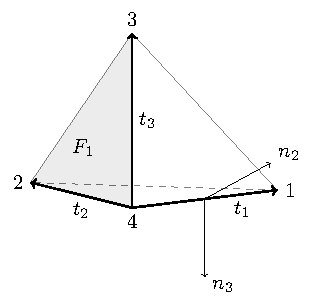
\includegraphics[width=6cm]{figures/tet.pdf}
\caption{Local coordinate formed by three edge vectors.}
\label{fig:localcoor}
\end{center}
\end{figure}
Let $\lambda_i(\boldsymbol x)$ be the $i$th barycentric coordinate with respect to the tetrahedron $K$ for $i=1,2,3,4$. Then $\lambda_i|_{F_i} = 0$ and $\nabla \lambda_i = - c_i \boldsymbol n_i$ for some $c_i>0$.

\begin{theorem}\label{lem:unisovlenHdivdivfem}
The degrees of freedom~\eqref{Hdivdivfem3ddof1}-\eqref{Hdivdivfem3ddof6} are unisolvent for $\boldsymbol \Sigma_{\ell,k}(K)$.
\end{theorem}
\begin{proof}
We first count the number of the degrees of freedom~\eqref{Hdivdivfem3ddof1}-\eqref{Hdivdivfem3ddof6}. Calculation of d.o.f.~\eqref{Hdivdivfem3ddof55} can be found in~\eqref{eq:dimsymx}.
The number of d.o.f.~\eqref{Hdivdivfem3ddof1}-\eqref{Hdivdivfem3ddof6} is
\begin{align*}
&24+18(\ell-1)+2[(\ell-1)(\ell-2)+(\ell+1)\ell] \\
&\quad+\frac{1}{6}(k^3-k)-4+\frac{1}{6}\ell(\ell-1)(5\ell+14) +\frac{1}{2}\ell(\ell-1) \\
=&\frac{1}{6}(5\ell^3+36\ell^2+67\ell+36)+\frac{1}{6}(k^3-k),
\end{align*}
which is same as $\dim\boldsymbol \Sigma_{\ell,k}(K)$ cf.~\eqref{eq:dimC}. 

%\begin{figure}[htbp]
%\begin{center}
%\includegraphics[width=5in]{figures/doftable.pdf}
%%\caption{The number of the degrees of freedom and the dimension of the space.}
%%\label{default}
%\end{center}
%\end{figure}


Take any $\boldsymbol \tau\in\boldsymbol \Sigma_{\ell,k}(K)$ and
suppose all the degrees of freedom~\eqref{Hdivdivfem3ddof1}-\eqref{Hdivdivfem3ddof6} vanish. We are going to prove the function $\boldsymbol \tau = 0$. 
Using the local coordinate sketched in Fig.~\ref{fig:localcoor}, we can expand $\boldsymbol \tau$ as
\[
\bs\tau=\sum_{i,j=1}^3\tau_{ij}\boldsymbol t_i\boldsymbol t_j^{\intercal} \quad\textrm{with}\quad \tau_{ij}=\frac{\boldsymbol n_i^{\intercal}\bs\tau\boldsymbol n_j}{(\boldsymbol t_i^{\intercal}\boldsymbol n_i)(\boldsymbol t_j^{\intercal}\boldsymbol n_j)}.
\]
As $\boldsymbol \tau$ is symmetric, $\tau_{ij} = \tau_{ji}$. 
By~\eqref{eq:20200707-21}, it follows
\[
\tau_{ii}|_{F_i}=\boldsymbol n_i^{\intercal}\bs\tau\boldsymbol n_i|_{F_i}=0, \quad i = 1,2,3.
\]
Thus there exists $q_{\ell-1}\in \mathbb P_{\ell-1}(K)$ satisfying $\tau_{ii}=\lambda_iq_{\ell-1}$ for $i=1,2,3$.
Taking $\boldsymbol \varsigma = q_{\ell-1}\boldsymbol n_i\boldsymbol n_i^{\intercal}$ in~\eqref{eq:20200707-3} will produce 
\begin{equation}\label{eq:diagonal}
\tau_{ii}=0, \quad i = 1,2,3.
\end{equation}
Namely the diagonal of $\boldsymbol \tau$ is zero.
So far, in the chosen coordinate, $\boldsymbol n_4^{\intercal}\bs\tau\boldsymbol n_4 = 0$ has no simple formulation and will be used later on.

On the other hand, from~\eqref{eq:20200707-1} we have $\Pi_{F_1}(\bs\tau\boldsymbol n_1)\in H_0(\div_{F_1}, F_1) $.
As $\boldsymbol n_1^{\intercal}\boldsymbol \tau \boldsymbol n_1 = \tau_{11} = 0$ in $K$ cf.~\eqref{eq:diagonal}, it follows $\partial_{n_1}(\boldsymbol n_1^{\intercal}\boldsymbol \tau \boldsymbol n_1)|_{F_1}=0$. Therefore~\eqref{eq:20200707-22} becomes
%$$\boldsymbol n_1^{\intercal} \boldsymbol \div\boldsymbol \tau |_{F_1}=\div(\boldsymbol\tau \boldsymbol n_1)|_{F_1}=\div(\Pi_{F_1}(\boldsymbol\tau \boldsymbol n_1))|_{F_1}=\div_{F_1}(\boldsymbol\tau \boldsymbol n_1)|_{F_1},
%$$
%we obtain from~\eqref{eq:20200707-22} that
\[
2\div_{F_1}(\boldsymbol\tau \boldsymbol n_1)|_{F_1}=0.
\]
Hence there exists $q_{\ell-2}\in \mathbb P_{\ell-2}(F_1)$ such that $\boldsymbol n_1\times(\boldsymbol\tau \boldsymbol n_1)=\nabla_{F_1}(b_{F_1}q_{\ell-2})$, 
where $b_{F_1}$ is the cubic bubble function on face $F_1$.
Together with~\eqref{Hdivdivfem3ddof6} and the fact $\div_{F_1}(\boldsymbol x\mathbb P_{\ell-2}(F_1))=\mathbb P_{\ell-2}(F_1)$, 
we get $(\boldsymbol n_1\times(\boldsymbol\tau \boldsymbol n_1))|_{F_1}=\boldsymbol 0$.
Thus $(\boldsymbol\tau \boldsymbol n_1)|_{F_1}=\boldsymbol 0$.
Then there exists $\boldsymbol q_{\ell-1}\in \mathbb P_{\ell-1}(K;\mathbb R^3)$ such that $\boldsymbol\tau \boldsymbol n_1=\lambda_1\boldsymbol q_{\ell-1}$,  combined with~\eqref{eq:20200707-3} yields $\boldsymbol\tau \boldsymbol n_1=\boldsymbol 0$. That is the first row of $\boldsymbol \tau$ is zero, i.e. $\tau_{11}=\tau_{12}=\tau_{13}=0$. 

By the symmetry, now
$
\bs\tau=2\tau_{23}\sym(\boldsymbol t_2\boldsymbol t_3^{\intercal})
$. Multiplying $\bs\tau$ by $\boldsymbol n_4$ from both sides and restricting to $F_4$, we have
\[
\tau_{23}|_{F_4}=\frac{1}{2}\frac{\boldsymbol n_4^{\intercal}\bs\tau\boldsymbol n_4}{(\boldsymbol t_2^{\intercal}\boldsymbol n_4)(\boldsymbol t_3^{\intercal}\boldsymbol n_4)}|_{F_4}=0.
\]
The denominator is non-zero as $\boldsymbol t_2, \boldsymbol t_3$ are non tangential vectors of face $F_4$. 
Again there exists $q_{\ell-1}\in \mathbb P_{\ell-1}(K)$ satisfying $\tau_{23}=\lambda_4q_{\ell-1}$.
Taking $\boldsymbol \varsigma=\sym(\boldsymbol t_2\boldsymbol t_3^{\intercal})q_{\ell-1}$ in~\eqref{eq:20200707-3} gives $\tau_{23}=0$. We thus have proved $\boldsymbol \tau = 0$ and consequently the unisolvence. 
\end{proof}

Due to~\eqref{Hdivdivfem3ddof4}, it is arduous to figure out the explicit basis functions of  $\boldsymbol \Sigma_{\ell,k}(K)$, which are dual to the degrees of freedom~\eqref{Hdivdivfem3ddof1}-\eqref{Hdivdivfem3ddof6}.
Alternatively we can hybridize the degrees of freedom~\eqref{Hdivdivfem3ddof4}, and use the basis functions of the standard Lagrange element~\cite{ChenHuang2020}. 
%We will discuss the hybridization in the next section.

\subsection{Polynomial bubble function spaces and the bubble complex}\label{sec:bubble}
%For the symmetric tensor space, it seems odd to have degrees of freedom not symmetric, as a face is singled out. 
Let
\begin{align*}
\mathring{\boldsymbol \Sigma}_{\ell,k}(K)&:=\{\boldsymbol  \tau\in\boldsymbol \Sigma_{\ell,k}(K): \textrm{all degrees of freedom~\eqref{Hdivdivfem3ddof1}-\eqref{Hdivdivfem3ddof4} vanish}\}.%,
%\\
%\mathring{\mathbb P}_{k-2}(K)&:=\mathbb P_{k-2}(K)/\mathbb P_{1}(K)
\end{align*}
Together with vanishing~\eqref{Hdivdivfem3ddof5}, we can  conclude that $\div\div \boldsymbol \tau = 0$. 
\begin{figure}[htbp]
\begin{center}
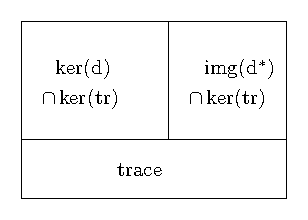
\includegraphics[width=5.4cm]{figures/femspacedecomposition.pdf}
\caption{Decomposition of a generic finite element space}
\label{fig:femdec}
\end{center}
\end{figure}
In view of Fig.~\ref{fig:femdec} and Lemma~\ref{lem:vanishdof}, the last two set of d.o.f.~\eqref{Hdivdivfem3ddof55}-\eqref{Hdivdivfem3ddof6} can be replaced by 
\begin{equation*}%\label{eq:divdivbubbledof}
(\boldsymbol \tau, \boldsymbol \varsigma)_K \quad \forall~\boldsymbol \varsigma\in \mathring{\boldsymbol \Sigma}_{\ell,k}(K) \cap \ker(\div\div),
\end{equation*}
Next we give characterization of $\mathring{\boldsymbol \Sigma}_{\ell,k}(K) \cap \ker(\div\div)$.

By the exactness of divdiv complex, if $\div\div \boldsymbol \tau = 0$ and $\tr(\boldsymbol \tau) = 0$, it is possible that $\boldsymbol \tau = \sym \curl \boldsymbol \sigma$ for some $\boldsymbol \sigma \in \boldsymbol B_{\ell+1}(\sym\curl, K;\mathbb T) : = \boldsymbol H_0(\sym \curl,K; \mathbb T)\cap \mathbb P_{\ell +1}(K;\mathbb T)$. 
%for each $K\in\mathcal T_h$.
We will give an explicit characterization of $\boldsymbol B_{\ell+1}(\sym\curl, K;\mathbb T)$, show $\mathring{\boldsymbol \Sigma}_{\ell,k}(K) \cap \ker(\div\div)= \sym \curl \boldsymbol B_{\ell+1}(\sym\curl, K;\mathbb T)$, and consequently get a set of computable and symmetric d.o.f..

We begin with a characterization of the trace of functions in $\boldsymbol H(\sym \curl,K; \mathbb T)$.
\begin{lemma} [Green's identity]\label{lm:Green}
Let $K$ be a polyhedron, and let $\boldsymbol  \tau\in \boldsymbol H^1(K; \mathbb M)$ and $\bs\sigma \in \boldsymbol H^1(K; \mathbb S)$. Then we have
\begin{align}
(\sym\curl\boldsymbol \tau, \boldsymbol \sigma)_K=(\boldsymbol \tau, \curl\boldsymbol \sigma)_K & - \sum_{F\in\mathcal F(K)}(\sym \Pi_F (\boldsymbol \tau\times\boldsymbol n)\Pi_F, \Pi_F \boldsymbol\sigma \Pi_F)_F \notag\\
& - \sum_{F\in\mathcal F(K)}(\boldsymbol n\cdot \boldsymbol \tau\times\boldsymbol n, \boldsymbol  n\cdot \boldsymbol\sigma \Pi_F)_F. \notag%\label{eq:greenidentitysymcurl}
\end{align}
\end{lemma}
\begin{proof}
As $\boldsymbol \sigma$ is symmetric,
\begin{align*}
(\sym\curl\boldsymbol \tau, \boldsymbol \sigma)_K&= (\curl\boldsymbol \tau, \boldsymbol \sigma)_K = (\boldsymbol \tau, \curl \boldsymbol \sigma)_K - (\boldsymbol \tau \times \boldsymbol n, \boldsymbol \sigma)_{\partial K}.
\end{align*}
%Note that due to our notation there  is  a negative sign on $\boldsymbol \tau \times \boldsymbol n$  
On each face, we expand the boundary term
\begin{align*}
(\boldsymbol \tau\times \boldsymbol n, \boldsymbol \sigma)_{F} = (\Pi_F (\boldsymbol \tau\times \boldsymbol n)\Pi_F, \Pi_F \boldsymbol\sigma \Pi_F)_F + (\boldsymbol n\cdot \boldsymbol \tau\times\boldsymbol n , \boldsymbol  n\cdot \boldsymbol\sigma \Pi_F)_F.
\end{align*}
Then we use the fact $\Pi_F \boldsymbol\sigma \Pi_F$ is symmetric to arrive the desired identity. 
\end{proof}

Based on the Green's identity, we introduce the following trace operators for $\boldsymbol H(\sym\curl)$ space
\begin{enumerate}
\item $\tr_1(\boldsymbol \tau) := \Pi_F \sym (\boldsymbol\tau\times\boldsymbol n)\Pi_F$,

 \item $\tr_1^{\bot}(\boldsymbol \tau) := \boldsymbol n \times \sym (\boldsymbol\tau\times\boldsymbol n)\times \boldsymbol n$,

 \item $\tr_2(\boldsymbol \tau) := \boldsymbol n\cdot \boldsymbol \tau\times\boldsymbol n$.
\end{enumerate}
Both $\tr_1(\boldsymbol \tau)$ and $\tr_1^{\bot}(\boldsymbol \tau)$ are symmetric tensors on each face and $\tr_2(\boldsymbol \tau)$ is a vector function. Obviously $\tr_1(\boldsymbol \tau) = 0$ if and only if  $\tr_1^{\bot}(\boldsymbol \tau) = 0$  as   $\tr_1^{\bot}(\boldsymbol \tau)$ is just a rotation of $\tr_1(\boldsymbol \tau)$.
%$$\tr(\boldsymbol \tau) = \{\boldsymbol n\times \sym(\boldsymbol\tau\times\boldsymbol n)\times\boldsymbol n, \boldsymbol n\cdot \boldsymbol \tau\times\boldsymbol n \}.$$
%In this subsection, we will show a polynomial bubble subcomplex of the divdiv complex, and one alternative of the interior degrees of freedom~\eqref{Hdivdivfem3ddof5}-\eqref{Hdivdivfem3ddof6}.
%
%
%
%For $\boldsymbol \sigma = \sym\curl \, \boldsymbol\tau$ with $\boldsymbol\tau\in\boldsymbol H^2(K;\mathbb M)$, Lemma~\ref{lm:tracerelation} suggests that 
%$$
%(\boldsymbol n\cdot \boldsymbol \tau\times\boldsymbol n)|_F\in \boldsymbol H(\div_F, F), \quad\Pi_F\sym(\boldsymbol\tau\times\boldsymbol n)\Pi_F\in \boldsymbol H(\div_F\div_F, F;\mathbb S).
%$$
%By the degrees of freedom of Raviart-Thomas element~\cite{RaviartThomas1977} and divdiv element in two dimensions~\cite{ChenHuang2020}, we list the following identities for later uses
%%For $\div_F$ and $\div_F\div_F$ elements on face $F$, the boundary edge degree freedom are simplified as
%\begin{equation}\label{eq:symcurltracepart1}
%(\boldsymbol n\cdot \boldsymbol \tau\times\boldsymbol n)\boldsymbol n_{F,e}=\boldsymbol n_{F}^{\intercal}\boldsymbol\tau\boldsymbol t_{F,e},
%\end{equation}
%\begin{equation}\label{eq:symcurltracepart2}
%(\boldsymbol n\cdot \boldsymbol \tau\times\boldsymbol n)\boldsymbol t_{F,e}=-\boldsymbol n_{F}^{\intercal}\boldsymbol\tau\boldsymbol n_{F,e},
%\end{equation}
%\begin{equation}\label{eq:symcurltracepart3}
%\boldsymbol n_{F,e}^{\intercal}(\Pi_F\sym(\boldsymbol\tau\times\boldsymbol n)\Pi_F)\boldsymbol n_{F,e}=\boldsymbol n_{F,e}^{\intercal}\sym(\boldsymbol\tau\times\boldsymbol n)\boldsymbol n_{F,e}= \boldsymbol n_{F,e}^{\intercal}\boldsymbol\tau\boldsymbol t_{F,e},
%\end{equation}
%\begin{equation}\label{eq:symcurltracepart4}
% \boldsymbol  t_{F,e}^{\intercal}\Pi_F\sym(\boldsymbol\tau\times\boldsymbol n)\Pi_F\boldsymbol  t_{F,e}=\boldsymbol  t_{F,e}^{\intercal}(\boldsymbol\tau\times\boldsymbol n)\boldsymbol  t_{F,e}=-\boldsymbol  t_{F,e}^{\intercal}\boldsymbol\tau\boldsymbol  n_{F,e},
% \end{equation}
% \begin{align}
% \boldsymbol  t_{F,e}^{\intercal}\Pi_F\sym(\boldsymbol\tau\times\boldsymbol n)\Pi_F\boldsymbol  n_{F,e}&=\frac{1}{2}\big(\boldsymbol  t_{F,e}^{\intercal}(\boldsymbol\tau\times\boldsymbol n)\boldsymbol  n_{F,e} + \boldsymbol  n_{F,e}^{\intercal}(\boldsymbol\tau\times\boldsymbol n)\boldsymbol  t_{F,e}\big) \notag\\
% &=\frac{1}{2}(\boldsymbol  t_{F,e}^{\intercal}\boldsymbol\tau\boldsymbol  t_{F,e} - \boldsymbol  n_{F,e}^{\intercal}\boldsymbol\tau\boldsymbol  n_{F,e} ). \label{eq:symcurltracepart5}
% \end{align}
%
Using the trace operators, $\boldsymbol H(\sym\curl)$ polynomial bubble function space can be defined as
\begin{align*}
\boldsymbol B_{\ell+1}(\sym\curl, K;\mathbb T):=\{&  
\bs\tau\in\mathbb P_{\ell+1}(K;\mathbb T):(\boldsymbol n\cdot \boldsymbol \tau\times\boldsymbol n)|_F=\bs0, \\
&(\boldsymbol n\times \sym(\boldsymbol\tau\times\boldsymbol n)\times\boldsymbol n)|_F=\bs0\quad\forall~F\in\mathcal F(K)
\}.
\end{align*}

We shall give an explicit characterization of $\boldsymbol B_{\ell+1}(\sym\curl, K;\mathbb T)$. 
\begin{lemma}\label{lem:symcurlbubbleedgevanish}
Let $\bs\tau\in \boldsymbol B_{\ell+1}(\sym\curl, K;\mathbb T)$. It holds
\begin{equation}\label{eq:edge}
\bs\tau|_e=\boldsymbol 0\quad\forall~e\in\mathcal E(K).
\end{equation}
\end{lemma}
\begin{proof}
It is straightforward to verify~\eqref{eq:edge} on the reference tetrahedron for which $\boldsymbol e = (1,0,0)$ and two normal vectors of the face containing $\boldsymbol e$ is $\boldsymbol n_1= (1,0,0)$ and $\boldsymbol n_2=(0,0,1)$. To avoid complicated transformation of trace operators, we provide a proof using an intrinsic basis of $\mathbb T$ on $K$. 

Take any edge $e\in\mathcal E(K)$ with the tangential vector $\boldsymbol t$. Let $\boldsymbol n_1$ and $\boldsymbol n_2$ be the unit outward normal vectors of two faces sharing edge $e$. Set $\boldsymbol s_i:=\boldsymbol t\times\boldsymbol n_i$ for $i=1,2$.
By direction computation, we get on edge $e$ for $i=1,2$ that
$$
\boldsymbol n_i^{\intercal}\bs\tau\boldsymbol t=(\boldsymbol n_i\cdot\bs\tau\times\boldsymbol n_i)\cdot\boldsymbol s_i=0,
$$
$$
\boldsymbol n_i^{\intercal}\bs\tau\boldsymbol s_i=-(\boldsymbol n_i\cdot\bs\tau\times\boldsymbol n_i)\cdot\boldsymbol t=0,
$$
$$
\boldsymbol t^{\intercal}\bs\tau\boldsymbol t - \boldsymbol s_i^{\intercal}\bs\tau\boldsymbol s_i=2\boldsymbol t\cdot \sym(\boldsymbol\tau\times\boldsymbol n_i)\cdot\boldsymbol s_i=2\boldsymbol s_i\cdot(\boldsymbol n_i\times \sym(\boldsymbol\tau\times\boldsymbol n_i)\times\boldsymbol n_i)\cdot\boldsymbol t=0,
$$
$$
\boldsymbol t^{\intercal}\bs\tau\boldsymbol s_i=-\boldsymbol t\cdot \sym(\boldsymbol\tau\times\boldsymbol n_i)\cdot\boldsymbol t=\boldsymbol s_i\cdot(\boldsymbol n_i\times \sym(\boldsymbol\tau\times\boldsymbol n_i)\times\boldsymbol n_i)\cdot\boldsymbol s_i=0.
$$
Both $\textrm{span}\{\boldsymbol s_1, \boldsymbol s_2\}$ and $\textrm{span}\{\boldsymbol n_1, \boldsymbol n_2\}$ form the same normal vector space of edge $e$, then the last identity implies
$$
\boldsymbol t^{\intercal}\bs\tau\boldsymbol n_i=0.
$$
% $$
% \boldsymbol n_i^{\intercal}\bs\tau\boldsymbol t=\boldsymbol n_i^{\intercal}\bs\tau\boldsymbol s_i=\boldsymbol t^{\intercal}\bs\tau\boldsymbol n_i=\boldsymbol t^{\intercal}\bs\tau\boldsymbol t - \boldsymbol s_i^{\intercal}\bs\tau\boldsymbol s_i=0\; \textrm{ on edge } e \;\textrm{ for } i=1,2.
% $$
Then it is sufficient to prove the eight trace-free tensors 
\begin{equation}\label{eq:nst}
\boldsymbol n_1\boldsymbol t^{\intercal},\; \boldsymbol n_2\boldsymbol t^{\intercal},\; \boldsymbol n_1\boldsymbol s_1^{\intercal},\; \boldsymbol n_2\boldsymbol s_2^{\intercal},\; \boldsymbol t\,\boldsymbol n_1^{\intercal},\; \boldsymbol t\,\boldsymbol n_2^{\intercal},\; \boldsymbol t\,\boldsymbol t^{\intercal}-\boldsymbol s_1\boldsymbol s_1^{\intercal},\; \boldsymbol t\,\boldsymbol t^{\intercal}-\boldsymbol s_2\boldsymbol s_2^{\intercal}
\end{equation}
are linear independent. Assume there exist $c_i\in\mathbb R$, $i=1,\cdots,8$ such that 
\begin{align*}
c_1\boldsymbol n_1\boldsymbol t^{\intercal} + c_2\boldsymbol n_2\boldsymbol t^{\intercal} + c_3\boldsymbol n_1\boldsymbol s_1^{\intercal} + c_4\boldsymbol n_2\boldsymbol s_2^{\intercal} + c_5\boldsymbol t\,\boldsymbol n_1^{\intercal} + c_6\boldsymbol t\,\boldsymbol n_2^{\intercal}&\\+c_7(\boldsymbol t\,\boldsymbol t^{\intercal}-\boldsymbol s_1\boldsymbol s_1^{\intercal}) + c_8(\boldsymbol t\,\boldsymbol t^{\intercal}-\boldsymbol s_2\boldsymbol s_2^{\intercal})&=\bs0.
\end{align*}
Multiplying the last equation by $\boldsymbol t$ from the right and left respectively, we obtain
$$
c_1\boldsymbol n_1 + c_2\boldsymbol n_2 + (c_7+c_8)\boldsymbol t=\bs0, \quad c_5\boldsymbol n_1^{\intercal} + c_6\boldsymbol n_2^{\intercal} + (c_7+c_8)\boldsymbol t^{\intercal}=\bs0.
$$
Hence $c_1=c_2=c_5=c_6=c_7+c_8=0$, which yields
$$
c_3\boldsymbol n_1\boldsymbol s_1^{\intercal} + c_4\boldsymbol n_2\boldsymbol s_2^{\intercal} + c_7(\boldsymbol s_2\boldsymbol s_2^{\intercal}-\boldsymbol s_1\boldsymbol s_1^{\intercal})=\bs0.
$$
Multiplying the last equation by $\boldsymbol n_1$ from the right, it follows
$$
(\boldsymbol s_2\cdot\boldsymbol n_1)(c_4\boldsymbol n_2 + c_7\boldsymbol s_2)=\bs0.
$$
As a result $c_4=c_7=0$, and then $c_3=0$.
\end{proof}

We write $\mathbb P_{\ell+1}(K;\mathbb T)$ as $\mathbb P_{\ell+1}(K)\otimes \mathbb T$ and use the barycentric coordinate representation of a polynomial. That is a polynomial $p\in \mathbb P_{\ell+1}(K)$ has a unique representation in terms of
\begin{equation}\label{eq:bary}
 p = \lambda_{1}^{\alpha_1}\lambda_{2}^{\alpha_2}\lambda_{3}^{\alpha_3}\lambda_{4}^{\alpha_4}, \quad \sum_{i=1}^4\alpha_i = \ell+1, \alpha_i \in \mathbb N.
\end{equation}
Lemma~\ref{lem:symcurlbubbleedgevanish} implies that $p$ must contain a face bubble $b_F = \lambda_{i}\lambda_{j}\lambda_{k}$ where $(i,j,k)$ are three vertices of $F$. Otherwise, if $p = \lambda_i^{\alpha_i}\lambda_j^{\alpha_j}, \alpha_i + \alpha_j = \ell+1$, then $p$ is not zero on the edge $(i,j)$. 

We consider the subspace $b_F \mathbb P_{\ell-2}(K)\otimes \mathbb T$ and identify its intersection with $\ker(\tr)$. Due to the face bubble $b_F$, the polynomial is zero on the other faces. So we only need to consider the trace on face $F$. Without loss of generality, we can chose the coordinate s.t. $n_F = (0,0,1)$. Chose the canonical basis of $\mathbb T$ associated to this coordinate. Then by direct calculation to find out $\ker(\tr)\cap \mathbb T$ consists of
$$
\begin{pmatrix}
0 & 0 & 1 \\
0 & 0 & 0 \\
0 & 0 & 0
\end{pmatrix},
\begin{pmatrix}
0 & 0 & 0 \\
0 & 0 & 1 \\
0 & 0 & 0
\end{pmatrix},
\text{ and }
\begin{pmatrix}
1 & 0 & 0 \\
0 & 1 & 0 \\
0 & 0 & -2
\end{pmatrix}.
$$
Switch to an intrinsic basis, we obtain the following explicit characterization of $\boldsymbol B_{\ell + 1}(\sym\curl, K;\mathbb T)$.
\begin{lemma}
For each face $F$, we chose two unit tangent vectors $\boldsymbol t_1, \boldsymbol t_2$ s.t. $(\boldsymbol t_1, \boldsymbol t_2, \boldsymbol n_F)$ forms an orthonormal basis of $\mathbb R^3$. Then
\begin{equation}\label{eq:span1}
\boldsymbol B_{\ell+1}(\sym\curl, K;\mathbb T)  = {\rm span}\{ p b_F \psi_i^F, p\in \mathbb P_{\ell-2}(K), F\in \mathcal F(K), i = 1,2,3\},
\end{equation}
where the three bubble functions are:
$$
\psi_1^F = \boldsymbol t_1 \boldsymbol n_F^{\intercal}, \quad \psi_2^F = \boldsymbol t_2 \boldsymbol n_F^{\intercal}, \quad  \psi_3^F = \boldsymbol t_1  \boldsymbol t_1^{\intercal} +  \boldsymbol t_2  \boldsymbol t_2^{\intercal} - 2 \boldsymbol n_F  \boldsymbol n_F^{\intercal}.
$$
\end{lemma}
\begin{proof}
% For any $\boldsymbol u, \boldsymbol v, \boldsymbol w\in\mathbb R^3$, it is easy to see that on each face $F\in\mathcal F(K)$
%\begin{align*}
%\boldsymbol n\cdot (\boldsymbol u\otimes \boldsymbol v)\times\boldsymbol n &= (\boldsymbol u\cdot\boldsymbol n)(\boldsymbol v\times \boldsymbol n)^{\intercal},\\
%\boldsymbol n\times\sym((\boldsymbol u\otimes \boldsymbol v)\times\boldsymbol n)\times\boldsymbol n &= \sym((\boldsymbol u\times\boldsymbol n)\otimes(\boldsymbol n\times\boldsymbol v\times\boldsymbol n)).
%\end{align*}
Using the formulae~\eqref{eq:xuv}-\eqref{eq:xtimesuv}, by the direct calculation, we can easily show $\psi_i^F\in \ker(\tr)\cap \mathbb T$ for each face $F$ and $i=1,2,3$. As $\dim \ker(\tr)\cap \mathbb T = 3$, we conclude that
$$ \ker (\tr) \cap (b_F \mathbb P_{\ell-2}(K)\otimes \mathbb T) = {\rm span} \{ p b_F \psi_i^F, p\in \mathbb P_{\ell-2}(K), i = 1,2,3\}.$$
By Lemma~\ref{lem:symcurlbubbleedgevanish}  we know that 
$$
\ker(\tr)\cap (\mathbb P_{\ell+1}\otimes \mathbb T) =  \cup_F \ker(\tr)\cap (b_F \mathbb P_{\ell-2}(K)\otimes \mathbb T) 
$$
and thus~\eqref{eq:span1} follows. 
\end{proof}

We only give a generating set of the bubble function space as the $12$ constant matrices $\{ \psi_1^F, \psi_2^F, \psi_3^F, F\in \mathcal F(K)\}, $ are not linear independent. Next we find out a basis from this generating set. 
\begin{lemma}
Let $(i,j,k)$ be three vertices of face $F$ and $\mathbb P_{\ell-2}(F) = \{ \lambda_{i}^{\alpha_1}\lambda_{j}^{\alpha_2}\lambda_{k}^{\alpha_3}, \alpha_1+\alpha_2+\alpha_3 = \ell-2, \alpha_i\in \mathbb N, i=1,2,3\}$.
 Define $\boldsymbol B_{F,\ell + 1}: = b_F\mathbb P_{\ell-2}(F)\otimes {\rm span}\{ \psi_1^F, \psi_2^F, \psi_3^F\}$ and $\boldsymbol B_{K, \ell + 1} = b_K\mathbb P_{\ell-3}(K)\otimes {\rm span}\{ \psi_1^F, \psi_2^F, F\in \mathcal F(K)\}$. Then
\begin{equation}\label{eq:basisofB}
\boldsymbol B_{\ell+1}(\sym\curl, K;\mathbb T)  = \oplus_{F\in \mathcal F(K)} \boldsymbol B_{F,\ell + 1} \oplus \boldsymbol B_{K,\ell + 1},
\end{equation} 
and consequently
$$\dim \boldsymbol B_{\ell+1}(\sym\curl, K;\mathbb T)=\frac{2}{3}\ell(\ell-1)(2\ell+5)=\frac{1}{3}(4\ell^3+6\ell^2-10\ell).$$ 
\end{lemma}
\begin{proof}
The $12$ constant matrices $\{ \psi_1^F, \psi_2^F, \psi_3^F, F\in \mathcal F(K)\}$ are not linear independent as $\dim \mathbb T = 8$. Among them, $\{ \psi_1^F, \psi_2^F, F\in \mathcal F(K)\}$ forms a basis of $\mathbb T$ which can be proved as verifying the linear independence of~\eqref{eq:nst} in Lemma~\ref{lem:symcurlbubbleedgevanish} or see~\cite{HuLiang2020}. 

For each $p b_F$, with $p\in \mathbb P_{\ell - 2}(K)$, we can group into either $b_K\mathbb P_{\ell-3}(K)$ or $b_F\mathbb P_{\ell-2}(F)$  depending on if the polynomial $p|_F$ is zero or not, respectively. That is, for one fixed face $F$:
$$
b_F \mathbb P_{\ell - 2}(K) = b_F\mathbb P_{\ell-2}(F) \oplus b_K\mathbb P_{\ell-3}(K). 
$$
The sum is direct in view of the barycentric representation~\eqref{eq:bary} of a polynomial.
Then coupled with $\{\psi_i^F\}$, we get the basis~\eqref{eq:basisofB} of the bubble function space.

The dimension of $\boldsymbol B_{\ell+1}(\sym\curl, K;\mathbb T) $ is 
\begin{align*}
4\cdot 3 \cdot \dim\mathbb P_{\ell-2}(F) + 8 \dim\mathbb P_{\ell-3}(K) = \frac{1}{3}(4\ell^3+6\ell^2-10\ell),
\end{align*}
as required.
\end{proof}


%\subsection{Bubble complex}

% Define divdiv bubble function spaces
% $$
% \boldsymbol B_{\ell}(\div\div, K;\mathbb S):=\{\bs\tau\in\mathbb P_{\ell}(K;\mathbb S): \textrm{all degrees of freedom~\eqref{Hdivdivfem3ddof1}-\eqref{Hdivdivfem3ddof4} vanish}\}.
% $$
% We have
% \begin{align*}
% \dim\boldsymbol B_{\ell}(\div\div, K;\mathbb S)&=\frac{1}{6}\ell(\ell^2-1)-4+\frac{1}{6}\ell(\ell-1)(5\ell+14) +\frac{1}{2}\ell(\ell-1) \\
% &=\ell^3+2\ell^2-3\ell-4.
% \end{align*}

We then verify $\sym \curl \boldsymbol B_{\ell+1}(\sym\curl, K;\mathbb T) \subset \mathring{\boldsymbol \Sigma}_{\ell,k}(K)$ by verifying all boundary d.o.f. are vanished. 
\begin{lemma}\label{lem:symcurledgeprop}
Let $\bs\tau \in \boldsymbol B_{\ell+1}(\sym\curl, K;\mathbb T)$. Assume edge $e\in\mathcal E(K)$ is shared by faces $F_i$ and $F_j$. It holds $\boldsymbol  n_i^{\intercal}(\sym\curl\boldsymbol \tau )\boldsymbol n_j|_e=0$.
\end{lemma}
\begin{proof}
For the ease of notation, let $\boldsymbol \sigma=\sym\curl\boldsymbol \tau$. Suppose $\bs\tau=\sum\limits_{F\in\mathcal F(K)}\sum\limits_{l=1}^3q_{F,l} b_F \psi_l^F$ with $q_{F,l}\in \mathbb P_{\ell-2}(K)$.
By $b_F|_e=0$, we get
$$
\boldsymbol n_i^{\intercal}\boldsymbol \sigma\boldsymbol n_j|_e=\sum_{F\in\mathcal F(K)}\sum_{l=1}^3q_{F,l}|_e(\boldsymbol n_i^{\intercal} \sym\curl(b_F \psi_l^F)\boldsymbol n_j)|_e.
$$
Since $\lambda_i|_e=\lambda_j|_e=0$, we can see that $(\boldsymbol n_i\times\boldsymbol n_F\cdot\nabla b_F)|_e=(\boldsymbol n_j\times\boldsymbol n_F\cdot\nabla b_F)|_e=0$. Thus for $l=1,2$,
\begin{align*}
&\quad\;(\boldsymbol n_i^{\intercal} \sym\curl(b_F \psi_l^F)\boldsymbol n_j)|_e\\
&=-(\boldsymbol n_i\cdot(b_F \boldsymbol t_l\boldsymbol n_F)\times\nabla\cdot\boldsymbol n_j)|_e - (\boldsymbol n_j\cdot(b_F\boldsymbol t_l\boldsymbol n_F)\times\nabla\cdot\boldsymbol n_i)|_e \\
&=\boldsymbol n_i\cdot\boldsymbol t_l(\boldsymbol n_F\times\boldsymbol n_j\cdot\nabla b_F)|_e + \boldsymbol n_j\cdot\boldsymbol t_l(\boldsymbol n_F\times\boldsymbol n_i\cdot\nabla b_F)|_e\\
&=0.
\end{align*}

Next consider $l=3$. When $F\neq F_j$, the face bubble $b_F$ has a factor $\lambda_j$, which implies $(\boldsymbol n_j\times\nabla b_F)|_e=\bs0$. Thus
$$
(\boldsymbol n_i^{\intercal}\curl(b_F \psi_3^F)\boldsymbol n_j)|_e =-(\boldsymbol n_i\cdot(b_F \psi_3^F)\times\nabla\cdot\boldsymbol n_j)|_e=(\boldsymbol n_i\cdot\psi_3^F\cdot(\boldsymbol n_j\times\nabla b_F))|_e=0.
$$
When $F= F_j$, the face bubble $b_F$ has a factor $\lambda_i$. 
By the fact that $(\boldsymbol t_1, \boldsymbol t_2, \boldsymbol n_j)$ forms an orthonormal basis of $\mathbb R^3$,
%we have
\begin{align*}
\boldsymbol n_i\cdot\boldsymbol t_2(\boldsymbol t_2\times\boldsymbol n_j\cdot\nabla\lambda_i)&=\boldsymbol n_i\cdot(\boldsymbol n_j\times\boldsymbol t_1)(\boldsymbol t_1\cdot\nabla\lambda_i)=-(\boldsymbol t_1\cdot\nabla\lambda_i)(\boldsymbol n_j\times\boldsymbol n_i\cdot\boldsymbol t_1) \\
&=-\boldsymbol n_i\cdot\boldsymbol t_1(\boldsymbol n_j\times\nabla\lambda_i\cdot\boldsymbol t_1),
\end{align*}
which implies
$$
\boldsymbol n_i\cdot\boldsymbol t_1(\boldsymbol n_j\times\nabla\lambda_i\cdot\boldsymbol t_1) + \boldsymbol n_i\cdot\boldsymbol t_2(\boldsymbol n_j\times\nabla\lambda_i\cdot\boldsymbol t_2)=0.
$$
As a result,
$$
(\boldsymbol n_i^{\intercal}\curl(b_F \psi_3^F)\boldsymbol n_j)|_e = \boldsymbol n_i\cdot\boldsymbol t_1(\boldsymbol n_j\times\nabla b_F\cdot\boldsymbol t_1)|_e + \boldsymbol n_i\cdot\boldsymbol t_2(\boldsymbol n_j\times\nabla b_F\cdot\boldsymbol t_2)|_e=0.
$$
Similarly $(\boldsymbol n_j^{\intercal}\curl(b_F \psi_3^F)\boldsymbol n_i)|_e=0$ holds. Hence $(\boldsymbol n_i^{\intercal}\sym\curl(b_F \psi_3^F)\boldsymbol n_j)|_e=0$.

Therefore $\boldsymbol  n_i^{\intercal}\boldsymbol \sigma\boldsymbol n_j|_e=0$.
\end{proof}

Next we show the two traces $\tr_2(\bs \tau)$ is in $H(\div_F)$ and $\tr_1(\bs \tau)$ in $H(\div_F\div_F)$. 
\begin{lemma}\label{lm:tracerelation}
When $\boldsymbol \sigma = \sym\curl \, \boldsymbol\tau$ with $\boldsymbol\tau\in\boldsymbol H^2(K;\mathbb M)$, we can express the trace in terms of the differential operators on surface $F$ of $K$
\begin{align}
\label{eq:trace1} \boldsymbol n^{\intercal}\boldsymbol \sigma\boldsymbol n &=\div_F(\boldsymbol n\cdot \boldsymbol \tau\times\boldsymbol n),\\
\label{eq:trace2} \nabla_F^{\bot}\cdot(\boldsymbol n\times\boldsymbol \sigma\cdot\boldsymbol n)+\boldsymbol  n^{\intercal} \div\boldsymbol \sigma  &=-\mathrm{rot}_F\mathrm{rot}_F(\boldsymbol n\times \sym(\boldsymbol\tau\times\boldsymbol n)\times\boldsymbol n)\\
& = \div_F\div_F(\Pi_F \sym(\boldsymbol\tau\times\boldsymbol n) \Pi_F). \notag
\end{align}
%Therefore $\tr_1(\boldsymbol \tau)\in H_n^{-1/2}(\div; \partial K)$ and $\tr_2(\boldsymbol \tau) \in H_t^{-3/2}(\div\div; \partial K)$. 
\end{lemma}
\begin{proof}
By
\begin{align*}
\boldsymbol n^{\intercal}\boldsymbol\sigma\boldsymbol n&=\frac{1}{2}\boldsymbol n\cdot(\nabla\times(\boldsymbol\tau^{\intercal})-\boldsymbol\tau\times\nabla)\cdot\boldsymbol n=\frac{1}{2}\nabla_F^{\bot}\cdot(\boldsymbol\tau^{\intercal})\cdot\boldsymbol n + \frac{1}{2}\boldsymbol n\cdot\boldsymbol\tau\cdot\nabla_F^{\bot}
\end{align*}
and the fact $\nabla_F^{\bot}\cdot(\boldsymbol\tau^{\intercal})\cdot\boldsymbol n=\boldsymbol n\cdot\boldsymbol\tau\cdot\nabla_F^{\bot}$, we get
$$
\boldsymbol n^{\intercal}\boldsymbol\sigma\boldsymbol n=\boldsymbol n\cdot\boldsymbol\tau\cdot\nabla_F^{\bot}=\mathrm{rot}_F (\boldsymbol n\cdot\boldsymbol \tau \Pi_F).
$$
Then the identity~\eqref{eq:trace1} holds from~\eqref{eq:rotFdivF}.

Next we prove~\eqref{eq:trace2}. Employing~\eqref{eq:tangentialtrace} with $\boldsymbol v=\boldsymbol\tau^{\intercal}\cdot\boldsymbol n$,
\begin{align*}
\nabla_F^{\bot}\cdot(\boldsymbol n\times\boldsymbol \sigma\cdot\boldsymbol n) &=\frac{1}{2}\nabla_F^{\bot}\cdot\big(\boldsymbol n\times(\nabla\times(\boldsymbol\tau^{\intercal})-\boldsymbol\tau\times\nabla)\cdot\boldsymbol n\big) \\
 &=\frac{1}{2}\nabla_F^{\bot}\cdot\big(\boldsymbol n\times(\nabla\times(\boldsymbol\tau^{\intercal}\cdot\boldsymbol n))\big) + \frac{1}{2}\nabla_F^{\bot}\cdot(\boldsymbol n\times\boldsymbol\tau)\cdot\nabla_F^{\bot} \\
 &=\frac{1}{2}\nabla_F^{\bot}\cdot\big(\nabla(\boldsymbol n\cdot\boldsymbol\tau^{\intercal}\cdot\boldsymbol n) - \partial_n(\boldsymbol\tau^{\intercal}\cdot\boldsymbol n)\big) + \frac{1}{2}\nabla_F^{\bot}\cdot(\boldsymbol n\times\boldsymbol\tau)\cdot\nabla_F^{\bot} \\
 &=-\frac{1}{2}\nabla_F^{\bot}\cdot\big(\partial_n(\boldsymbol\tau^{\intercal}\cdot\boldsymbol n)\big) + \frac{1}{2}\nabla_F^{\bot}\cdot(\boldsymbol n\times\boldsymbol\tau)\cdot\nabla_F^{\bot}.
\end{align*}
On the other side, we have
\begin{align*}
\boldsymbol n\cdot \div\boldsymbol \sigma &=\boldsymbol  n\cdot\boldsymbol\sigma\cdot\nabla=\frac{1}{2}\boldsymbol n\cdot(\nabla\times(\boldsymbol\tau^{\intercal}))\cdot\nabla=\frac{1}{2}\nabla_F^{\bot}\cdot(\boldsymbol\tau^{\intercal})\cdot\nabla \\
&=\frac{1}{2}\nabla_F^{\bot}\cdot(\boldsymbol\tau^{\intercal})\cdot(\boldsymbol n\partial_n+\nabla_F)=\frac{1}{2}\nabla_F^{\bot}\cdot\big(\partial_n(\boldsymbol\tau^{\intercal}\cdot\boldsymbol n)\big) + \frac{1}{2}\nabla_F^{\bot}\cdot(\boldsymbol\tau^{\intercal})\cdot\nabla_F \\
&=\frac{1}{2}\nabla_F^{\bot}\cdot\big(\partial_n(\boldsymbol\tau^{\intercal}\cdot\boldsymbol n)\big) - \frac{1}{2}\nabla_F^{\bot}\cdot(\boldsymbol\tau^{\intercal}\times\boldsymbol n)\cdot\nabla_F^{\bot}.
\end{align*}
The sum of the last two identities gives
\begin{align*}
\nabla_F^{\bot}\cdot(\boldsymbol n\times\boldsymbol \sigma\cdot\boldsymbol n)+\boldsymbol  n\cdot \div\boldsymbol \sigma &=\nabla_F^{\bot}\cdot\sym(\boldsymbol n\times\boldsymbol\tau\Pi_F)\cdot\nabla_F^{\bot}.
\end{align*}
Therefore~\eqref{eq:trace2} follows from $\sym(\boldsymbol n\times\boldsymbol\tau\Pi_F)=-\boldsymbol  n\times \sym(\boldsymbol\tau\times\boldsymbol n)\times\boldsymbol n$.
\end{proof}

Note that $ \nabla_F^{\bot}\cdot(\boldsymbol n\times\boldsymbol \sigma\cdot\boldsymbol n)+\boldsymbol  n^{\intercal} \div\boldsymbol \sigma$ is an equivalent formulation of the second trace of $\boldsymbol \sigma$. 
%We shall not discuss more on the trace operator in the general setting but restrict to polynomial spaces. 
%
Combining Lemmas~\ref{lem:symcurledgeprop} and~\ref{lm:tracerelation} gives the following result.
\begin{lemma}\label{lm:symbubble}
It holds
\begin{equation}\label{eq:symcurlindivdivbubble}
\sym\curl \boldsymbol B_{\ell+1}(\sym\curl, K;\mathbb T) \subseteq (\mathring{\boldsymbol \Sigma}_{\ell,k}(K)\cap\ker(\div\div)).
\end{equation}
\end{lemma}
\begin{proof}
For $\boldsymbol \tau \in \boldsymbol B_{\ell+1}(\sym\curl, K;\mathbb T)$, by construction, $\boldsymbol n\cdot \boldsymbol \tau\times\boldsymbol n = 0$ and $\boldsymbol n\times \sym(\boldsymbol\tau\times\boldsymbol n)\times\boldsymbol n = 0$ on $\partial K$. Let $\boldsymbol \sigma = \sym \curl \boldsymbol \tau$. Then by Lemma~\ref{lm:tracerelation}, d.o.f.~\eqref{Hdivdivfem3ddof3}-\eqref{Hdivdivfem3ddof4} vanish. By Lemma~\ref{lem:symcurledgeprop},~\eqref{Hdivdivfem3ddof2} vanish. As $\boldsymbol \tau$ contains a face bubble, $\boldsymbol \sigma$  will have an  edge bubble function which means $\boldsymbol \sigma(\delta) = 0$ for all $\delta \in \mathcal V(K)$. Therefore  $\sym\curl \boldsymbol B_{\ell+1}(\sym\curl, K;\mathbb T) \subseteq \mathring{\boldsymbol \Sigma}_{\ell,k}(K)$. The property $\div\div (\sym \curl \boldsymbol \tau) = 0$ is from the divdiv complex.
\end{proof}

Indeed the $``\subseteq"$  in~\eqref{eq:symcurlindivdivbubble} can be changed to ``=". This will be clean after we present a bubble complex. 

\begin{lemma}\label{lem:divdivbubble}
For each $K\in\mathcal T_h$, it holds
\begin{equation}\label{eq:divdivL2local0}
\div\div\mathring{\boldsymbol \Sigma}_{\ell,k}(K)=\mathbb P_{k-2}(K)\cap \mathbb P_1^{\bot}(K),
\end{equation}
where $\mathbb P_1^{\bot}(K)$ is a subspace of $L^2(K)$ being orthogonal to $\mathbb P_1(K)$ with respect to the $L^2$-inner product $(\cdot, \cdot)_K$. Consequently
\begin{equation}\label{eq:dimdivdivbubble}
\dim(\mathring{\boldsymbol \Sigma}_{\ell,k}(K)\cap\ker(\div\div))=\frac{1}{6}\ell(\ell-1)(5\ell+17). 
\end{equation}
%That is for any $q\in\mathring{\mathbb P}_{k-2}(K)$, there exists $\bs\tau\in\mathring{\boldsymbol \Sigma}_{\ell,k}(K)$ such that
%\[
%\div\bs\div\bs\tau=q,\quad
%\]
\end{lemma}
\begin{proof}
From the integration by parts, it is obviously true that $\div\div\mathring{\boldsymbol \Sigma}_{\ell,k}(K)\subseteq\mathbb P_{k-2}(K)\cap \mathbb P_1^{\bot}(K)$.
On the other side, for any $v\in\mathbb P_{k-2}(K)\cap \mathbb P_1^{\bot}(K)$, due to the fact that $\div\div \boldsymbol H_0^2(K;\mathbb S)=L^2(K)\cap \mathbb P_1^{\bot}(K)$~\cite{CostabelMcIntosh2010}, 
there exists $\widetilde{\bs\tau}\in\boldsymbol H_0^2(K;\mathbb S)$ such that
\[
\div\div\widetilde{\bs\tau}=v. %,\quad \|\widetilde{\bs\tau}\|_{2,K}\lesssim \|q\|_{0,K}.
\]
Then take $\boldsymbol \tau \in\mathring{\boldsymbol \Sigma}_{\ell,k}(K)$ with the rest d.o.f. 
\begin{align*}
(\boldsymbol \tau-\widetilde{\bs\tau}, \boldsymbol \varsigma)_K=0&  \quad\forall~\boldsymbol \varsigma\in\nabla^2\mathbb P_{k-2}(K)\oplus\sym(\mathbb P_{\ell-2}(K; \mathbb T)\times\boldsymbol x), \\
((\boldsymbol \tau-\widetilde{\bs\tau})\boldsymbol n, \boldsymbol  n\times \boldsymbol x q)_{F_1}=0 &\quad\forall~q\in\mathbb P_{\ell-2}(F_1).
\end{align*}
Applying the Green's identity~\eqref{eq:greenidentitydivdiv}, we get
\[
(\div\div(\boldsymbol \tau-\widetilde{\bs\tau}), q)_K=0\quad\forall~q\in\mathbb P_{k-2}(K).
\]
This implies $\div\div\boldsymbol \tau=\div\div\widetilde{\bs\tau}=v$. Namely~\eqref{eq:divdivL2local0} holds.

An immediate result of~\eqref{eq:divdivL2local0} is
\begin{align*}
\dim(\mathring{\boldsymbol \Sigma}_{\ell,k}(K)\cap\ker(\div\div))& =\dim\mathring{\boldsymbol \Sigma}_{\ell,k}(K)-\dim\mathbb P_{k-2}(K)+4 \\
&=\frac{1}{6}\ell(\ell-1)(5\ell+14) +\frac{1}{2}\ell(\ell-1)\\
&=\frac{1}{6}\ell(\ell-1)(5\ell+17).
\end{align*}
\end{proof}


Define
$$
\boldsymbol B_{\ell+2}(K;\mathbb R^3):=\{\boldsymbol v\in\mathbb P_{\ell+2}(K;\mathbb R^3): \boldsymbol v|_{\partial K}=\bs0\}=b_K\mathbb P_{\ell-2}(K;\mathbb R^3).
$$
Now we are in the position to present the so-called bubble complex. 

\begin{theorem}\label{th:bubblecomplex}
The bubble function spaces for the divdiv complex
\begin{equation}\label{eq:divdivcomplex3dfembubble}
\resizebox{.92\hsize}{!}{$
0\xrightarrow{} \boldsymbol B_{\ell+2}(K;\mathbb R^3)\xrightarrow{\dev\grad} \boldsymbol B_{\ell+1}(\sym\curl, K;\mathbb T) \xrightarrow{\sym\curl} \mathring{\boldsymbol \Sigma}_{\ell,k}(K) \xrightarrow{\div{\div}} \mathbb P_{k-2}(K)\cap \mathbb P_1^{\bot}(K)\xrightarrow{}0
$}
\end{equation}
form an exact Hilbert complex. 
\end{theorem}
\begin{proof}
Take any $\boldsymbol v\in \boldsymbol B_{\ell+2}(K;\mathbb R^3)$ with $\boldsymbol v|_{\partial K}=\bs0$.
We have on each face $F\in\mathcal F(K)$,
\begin{equation}\label{eq:devgradtr1}
\boldsymbol n\cdot(\dev\grad\boldsymbol v)\times\boldsymbol n=\boldsymbol n\cdot(\grad\boldsymbol v)\times\boldsymbol n=-(\boldsymbol n\times\nabla)(\boldsymbol v\cdot\boldsymbol n)=\bs0,
\end{equation}
and
\begin{align}
\boldsymbol n\times \sym((\dev\grad\boldsymbol v)\times\boldsymbol n)\times\boldsymbol n&=\boldsymbol n\times \sym((\grad\boldsymbol v)\times\boldsymbol n)\times\boldsymbol n \notag\\
&=-\boldsymbol n\times \sym(\boldsymbol v\nabla_F^{\bot})\times\boldsymbol n \notag\\
&=-\boldsymbol n\times \sym((\Pi_F\boldsymbol v)\nabla_F^{\bot})\times\boldsymbol n=\bs0. \label{eq:devgradtr2}
\end{align}
Hence $\dev\grad\boldsymbol B_{\ell+2}(K;\mathbb R^3)\subseteq\boldsymbol B_{\ell+1}(\sym\curl, K;\mathbb T)\cap\ker(\sym\curl)$.
Thanks to Lemma~\ref{lm:symbubble} and~\eqref{eq:divdivL2local0}, we conclude that ~\eqref{eq:divdivcomplex3dfembubble} is a complex.

We then verify the exactness from the left to the right.

\medskip
\noindent {\em 1. $\boldsymbol B_{\ell+1}(\sym\curl, K;\mathbb T)\cap\ker(\sym\curl)=\dev\grad\boldsymbol B_{\ell+2}(K;\mathbb R^3)$, i.e. if $\sym\curl\boldsymbol \tau = \boldsymbol 0$ and $\bs\tau\in \boldsymbol B_{\ell+1}(\sym\curl, K;\mathbb T)$, then there exists a $\boldsymbol v\in\boldsymbol B_{\ell+2}(K;\mathbb R^3)$, s.t. $\boldsymbol \tau = \dev\grad\boldsymbol v$}. 

Firstly, by the exactness of the polynomial divdiv complex~\eqref{eq:divdivcomplex3dPoly}, there exists $\boldsymbol v\in\mathbb P_{\ell+2}(K;\mathbb R^3)$ such that $\bs\tau=\dev\grad\boldsymbol v$. As $\bs{RT}=\ker(\dev\grad)$, we  can further impose constraint $\int_F \boldsymbol v\cdot\boldsymbol n=0$ for each $F\in\mathcal F(K)$.
By~\eqref{eq:devgradtr1}, we get $ \boldsymbol v\cdot\boldsymbol n \mid _F\in\mathbb P_0(F)$. Hence $\boldsymbol v\cdot\boldsymbol n|_F=0$, which indicates $\boldsymbol v(\delta)=\bs0$ for each vertex $\delta\in\mathcal V(K)$.
By~\eqref{eq:devgradtr2}, we obtain $\sym((\Pi_F\boldsymbol v)\nabla_F^{\bot})=\bs0$, i.e. $\Pi_F\boldsymbol v\in\mathbb P_0(F;\mathbb R^2)+(\Pi_F\boldsymbol x)\mathbb P_0(F)$. This combined with $\boldsymbol v(\delta)=\bs0$ for each vertex $\delta\in\mathcal V(F)$ means $\Pi_F\boldsymbol v=\bs0$, and then $\boldsymbol v|_F=\bs0$ for each $F\in \mathcal F(K)$. Thus $\boldsymbol v\in \boldsymbol B_{\ell+2}(K;\mathbb R^3)$.

\medskip
\noindent {\em 2. $\sym\curl\boldsymbol B_{\ell+1}(\sym\curl, K;\mathbb T)=\mathring{\boldsymbol \Sigma}_{\ell,k}(K)\cap\ker(\div\div)$}. 

By step 1, we acquire
\begin{align}
&\quad\,\dim\sym\curl\boldsymbol B_{\ell+1}(\sym\curl, K;\mathbb T) \notag \\
&=\dim\boldsymbol B_{\ell+1}(\sym\curl, K;\mathbb T)-\dim\boldsymbol B_{\ell+2}(K;\mathbb R^3) \notag  \\
&=\dim\boldsymbol B_{\ell+1}(\sym\curl, K;\mathbb T)-\dim\mathbb P_{\ell-2}(K;\mathbb R^3) \notag \\
&=\frac{1}{6}\ell(\ell-1)(5\ell+17) \label{eq:dimsymcurlB},
\end{align}
which together with~\eqref{eq:dimdivdivbubble} indicates
$$
\dim\sym\curl\boldsymbol B_{\ell+1}(\sym\curl, K;\mathbb T)=\dim(\mathring{\boldsymbol \Sigma}_{\ell,k}(K)\cap\ker(\div\div)).$$ 
Together with~\eqref{eq:symcurlindivdivbubble} implies $\sym\curl\boldsymbol B_{\ell+1}(\sym\curl, K;\mathbb T)=\mathring{\boldsymbol \Sigma}_{\ell,k}(K)\cap\ker(\div\div)$.

\medskip
\noindent {\em 3. $\div\div\mathring{\boldsymbol \Sigma}_{\ell,k}(K)=\mathbb P_{k-2}(K)\cap \mathbb P_1^{\bot}(K)$.}  This is~\eqref{eq:divdivL2local0} proved in Lemma~\ref{lem:divdivbubble}.

\medskip

Therefore complex~\eqref{eq:divdivcomplex3dfembubble} is exact.
\end{proof}

As a result of complex~\eqref{eq:divdivcomplex3dfembubble}, we can replace the degrees of freedom~\eqref{Hdivdivfem3ddof55}-\eqref{Hdivdivfem3ddof6} by
\begin{align}\label{Hdivdivfem3ddofbubble}
(\boldsymbol \tau, \boldsymbol \varsigma)_K & \quad\forall~\boldsymbol \varsigma\in\sym\curl\boldsymbol B_{\ell+1}(\sym\curl, K;\mathbb T).
\end{align}
The dimension of~\eqref{Hdivdivfem3ddofbubble} is counted in~\eqref{eq:dimsymcurlB}, which also matches the sum of~\eqref{Hdivdivfem3ddof55}-\eqref{Hdivdivfem3ddof6}. 

We summarize the unisolvence below.

\begin{corollary}\label{cor:unisovlenHdivdivfem2}
The degrees of freedom~\eqref{Hdivdivfem3ddof1}-\eqref{Hdivdivfem3ddof5} and~\eqref{Hdivdivfem3ddofbubble} are unisolvent for $\boldsymbol \Sigma_{\ell,k}(K)$.
\end{corollary}

Notice that although $\boldsymbol B_{\ell+1}(\sym\curl, K;\mathbb T)$ is in a symmetric form, cf.~\eqref{eq:basisofB}, the degrees of freedom~\eqref{Hdivdivfem3ddofbubble} is indeed not simpler than~\eqref{Hdivdivfem3ddof55}-\eqref{Hdivdivfem3ddof6} in computation as $\sym\curl\boldsymbol B_{\ell+1}(\sym\curl, K;\mathbb T)$ is much more complicated than polynomials on a face. 

\subsection{Two dimensional divdiv conforming finite elements}\label{sec:2D}
Recently we have constructed divdiv conforming finite elements in two dimensions in~\cite{ChenHuang2020}. Here we briefly review the results and compare to the three dimensional case. 

Let $F$ be a triangle. Take the space of shape functions
\begin{equation}\label{eq:2DSigma}
\boldsymbol \Sigma_{\ell,k}(F):= \mathbb C_{\ell}(F;\mathbb S)\oplus\mathbb C_k^{\oplus}(F;\mathbb S)
\end{equation}
with $k\geq 3$ and $\ell\geq \max\{k-1, 3\}$ and 
\[
\mathbb C_{\ell}(F; \mathbb S)=\sym \curl_F \, \mathbb  P_{\ell +1}(F; \mathbb R^2),\quad \mathbb C_k^{\oplus}(F; \mathbb S)=\boldsymbol  x\boldsymbol  x^{\intercal}\mathbb P_{k-2}(F).
\]
Here the polynomial space for $\boldsymbol H(\sym \curl, F; \mathbb R^2)$ is the vector space not a tensor space, which simplifies the construction significantly. 

The degrees of freedom are given by
\begin{align}
%v(\delta) & \quad\textrm{for each } \delta\in \mathcal V(K), \label{H1ncfmdof1}\\
\boldsymbol \tau (\delta) & \quad\forall~\delta\in \mathcal V(F), \label{Hdivdivfemdof1}\\
(\boldsymbol  n_{e}^{\intercal}\boldsymbol \tau\boldsymbol  n_{e}, q)_e & \quad\forall~q\in\mathbb P_{\ell-2}(e),  e\in\mathcal E(F),\label{Hdivdivfemdof2}\\
(\partial_{t}(\boldsymbol  t^{\intercal}\boldsymbol \tau\boldsymbol  n_{e})+\boldsymbol  n_{e}^{\intercal}\div_F\boldsymbol \tau, q)_e & \quad\forall~q\in\mathbb P_{\ell-1}(e),  e\in\mathcal E(F),\label{Hdivdivfemdof3}\\
(\boldsymbol \tau, \boldsymbol \varsigma)_F & \quad\forall~\boldsymbol \varsigma\in\nabla_F^2\mathbb P_{k-2}(F), \label{Hdivdivfemdof4}\\
(\boldsymbol \tau, \boldsymbol \varsigma)_F & \quad\forall~\boldsymbol \varsigma\in \sym (\boldsymbol x^{\bot} \mathbb P_{\ell-2}(F;\mathbb R^2)). \label{Hdivdivfemdof5}
%\sym\curl(b_K\mathbb P_{\ell-2}(K;\mathbb R^2))
\end{align}
Here to avoid confusion with three dimensional version, we use $\bs n_e$ to emphasize it is a normal vector of edge vector $e$. 

The unisolvence is again better understood with the help of Fig.~\ref{fig:femdec}. 
By the vanishing degrees of freedom~\eqref{Hdivdivfemdof1}-\eqref{Hdivdivfemdof3}, the trace is vanished. Then together with the vanishing ~\eqref{Hdivdivfemdof4}, $\div \div \boldsymbol \tau = 0$. The rest is to identify the intersection of the bubble space and the kernel of $\div\div$. Define
\begin{align*}
\mathring{\boldsymbol \Sigma}_{\ell,k}(F)&:=\{\boldsymbol  \tau\in\boldsymbol \Sigma_{\ell,k}(F): \textrm{all degrees of freedom~\eqref{Hdivdivfemdof1}-\eqref{Hdivdivfemdof3} vanish}\}.%,
\end{align*}
It turns out the space $\mathring{\boldsymbol \Sigma}_{\ell,k}(F)\cap \ker(\div_F\div_F)$ is much simpler in two dimensions. 

The key is the following formulae on the trace $\tr_2$. 
\begin{lemma}\label{lm:tauv}
When $\boldsymbol  \tau = \sym \curl_F \, \boldsymbol  v$, we have
\begin{align}
\label{eq:trace2-2d} \partial_{t}(\boldsymbol  t^{\intercal}\boldsymbol \tau\boldsymbol  n_{e})+\boldsymbol  n_{e}^{\intercal}\div_F\boldsymbol \tau & =  \partial_t(\boldsymbol  t^{\intercal}\partial_t\boldsymbol  v).
\end{align}
\end{lemma}
\begin{proof}
Since $\div_F \curl_F \, \boldsymbol  v = 0$, we have
$$\boldsymbol  n^{\intercal}\div_F\boldsymbol \tau  = \frac{1}{2}\boldsymbol  n_{e}^{\intercal} \div_F ( \curl_F \, \boldsymbol  v)^{\intercal} = \frac{1}{2}\boldsymbol  n_{e}^{\intercal} \curl_F \div_F \boldsymbol  v =  \frac{1}{2} \partial_t \div_F \boldsymbol  v.$$
As $\div_F\boldsymbol  v = {\rm trace} (\nabla_F\boldsymbol  v)$ is invariant to the rotation, we can write it as
$$
\div_F \boldsymbol  v = \boldsymbol  t^{\intercal}\nabla_F\boldsymbol  v \boldsymbol  t + \boldsymbol  n_{e}^{\intercal}\nabla_F\boldsymbol  v \boldsymbol  n_{e} =  \boldsymbol  t^{\intercal}\partial_t\boldsymbol  v + \boldsymbol  n_{e}^{\intercal}\partial_n\boldsymbol  v.
$$
Then
$$
 \partial_{t}(\boldsymbol  t^{\intercal}\boldsymbol \tau\boldsymbol  n_{e})+\boldsymbol  n_{e}^{\intercal}\div_F\boldsymbol \tau  =\frac{1}{2}\partial_t[  \boldsymbol  t^{\intercal}\partial_t\boldsymbol  v -  \boldsymbol  n_{e}^{\intercal}\partial_n\boldsymbol  v + \div_F\boldsymbol  v]  =  \partial_t  (\boldsymbol  t^{\intercal}\partial_t\boldsymbol  v),
 $$
 i.e.~\eqref{eq:trace2-2d} holds.
\end{proof}


\begin{lemma}
The following bubble complex: 
\begin{equation*}%\label{eq:divdivbubble}
%\resizebox{.92\hsize}{!}{$
\bs0\xrightarrow{\subset} b_F\mathbb P_{\ell-2}(F;\mathbb R^2)\xrightarrow{\sym\curl_F} \mathring{\boldsymbol \Sigma}_{\ell,k}(F)\xrightarrow{\div_F\div_F} \mathbb P_{k-2}(F)\cap\mathbb P_1^{\perp}(F)\xrightarrow{}0
%$}
\end{equation*}
is exact.
\end{lemma}
\begin{proof}
The fact $\div_F\div_F: \mathring{\boldsymbol \Sigma}_{\ell,k}(F) \to \mathbb P_{k-2}(F)\cap\mathbb P_1^{\perp}(F)$ is surjective can be proved similarly to Lemma~\ref{lem:divdivbubble}. 

For $\boldsymbol \tau \in \mathring{\boldsymbol \Sigma}_{\ell,k}(F)\cap\ker(\div_F\div_F)$, from the complex~\eqref{eq:divdivcomplexPolydouble2D}, we can find $\boldsymbol v\in \mathbb P_{\ell+1}(F)$ s.t. $\sym \curl_F \boldsymbol v = \boldsymbol \tau$.  We will prove $\boldsymbol v|_{\partial F} = \boldsymbol 0$. 

Since $\bs{RT}=\ker(\sym\curl_F)$, we can further impose constraint $\int_e \boldsymbol v\cdot\boldsymbol n_{e}=0$ for each $e\in\mathcal E(F)$. The fact $(\boldsymbol n_{e}^{\intercal}\boldsymbol \tau\boldsymbol  n_{e})|_{\partial F}=0$ implies
\[
\partial_t(\boldsymbol  n_{e}^{\intercal}\boldsymbol  v)|_{\partial F}= (\boldsymbol  n_{e}^{\intercal}\boldsymbol \tau\boldsymbol  n_{e})|_{\partial F}=0.
\]
Hence $\boldsymbol  n_{e}^{\intercal}\boldsymbol  v|_{\partial F}=0$.
%Hence $\boldsymbol  n^{\intercal}\boldsymbol  v|_e$ is constant on each edge $e\in\mathcal E(K)$.
%Then we can choose $\boldsymbol  v$ satisfying $\boldsymbol  n^{\intercal}\boldsymbol  v|_{\partial K}=0$.
This also means $\boldsymbol  v(\delta)=\boldsymbol 0$ for each $\delta\in\mathcal V(F)$.


By Lemma~\ref{lm:tauv}, since
\begin{equation*}%\label{eq:20200422}
\partial_{t}(\boldsymbol  t^{\intercal}\boldsymbol \tau\boldsymbol  n_{e})+\boldsymbol  n_{e}^{\intercal}\div_F\boldsymbol \tau= \partial_t(\boldsymbol  t^{\intercal}\partial_t\boldsymbol  v)
\end{equation*}
and $(\partial_{t}(\boldsymbol  t^{\intercal}\boldsymbol \tau\boldsymbol  n_{e})+\boldsymbol  n_{e}^{\intercal}\div_F\boldsymbol \tau)|_{\partial F}=0$, we acquire
\[
\partial_{tt}(\boldsymbol  t^{\intercal}\boldsymbol  v)|_{\partial F}=0.
\]
That is $\boldsymbol  t^{\intercal}\boldsymbol  v|_e\in\mathbb P_1(e)$ on each edge $e\in\mathcal E(F)$. Noting that $\boldsymbol  v(\delta)=\boldsymbol 0$ for each $\delta\in\mathcal V(F)$, we get $\boldsymbol t^{\intercal}\boldsymbol  v|_{\partial F}=0$ and consequently $\boldsymbol  v|_{\partial F}=\boldsymbol 0$, i.e., 
$$
\boldsymbol v = b_F\psi_{\ell-2},\quad \text{for some } \psi_{\ell-2} \in \mathbb P_{\ell-2}(F;\mathbb R^2).
$$
\end{proof}


We now prove the unisolvence as follows.

\begin{theorem}\label{thm:unisovlenHdivdivfem2D}
The degrees of freedom~\eqref{Hdivdivfemdof1}-\eqref{Hdivdivfemdof4} are unisolvent for $\boldsymbol \Sigma_{\ell,k}(F)$~\eqref{eq:2DSigma}.
\end{theorem}
\begin{proof}
We first count the number of the degrees of freedom~\eqref{Hdivdivfemdof1}-\eqref{Hdivdivfemdof4}  and the dimension of the space, i.e., $\dim\boldsymbol \Sigma_{\ell,k}(K)$.
Both of them are $$\ell^2+5\ell+3+\frac{1}{2}k(k-1).$$
Then suppose all the degrees of freedom~\eqref{Hdivdivfemdof1}-\eqref{Hdivdivfemdof4} applied to $\boldsymbol \tau$ vanish. We are going to prove the function $\boldsymbol \tau = 0$. 

By the vanishing degrees of freedom~\eqref{Hdivdivfemdof1}-\eqref{Hdivdivfemdof3}, the two traces are vanished. Together with~\eqref{Hdivdivfemdof4}, the Green's identity implies $\div_F\div_F \boldsymbol \tau = 0$. Then $$
\boldsymbol \tau = \sym \curl_{F}  (b_F\psi_{\ell-2}),\quad \text{for some } \psi_{\ell-2} \in \mathbb P_{\ell-2}(F;\mathbb R^2).
$$
We then use the fact $\rot_F: \sym(\boldsymbol x^{\perp}\mathbb P_{\ell-2}(F;\mathbb R^2)) \to  \mathbb P_{\ell-2}(F;\mathbb R^2)$ is bijection, cf. the complex~\eqref{eq:hessiancomplexPolydouble2D}, to find $\phi_{\ell-2}$ s.t. $\rot_F (\sym(\boldsymbol x^{\perp}\phi_{\ell-2})) = \psi_{\ell-2}$.
%
Finally we finish the unisolvence proof by choosing $\boldsymbol \varsigma = \sym (\boldsymbol x^{\perp} \phi_{\ell -2})$ in~\eqref{Hdivdivfemdof5}. The fact 
$$
(\boldsymbol \tau, \boldsymbol \varsigma)_F = (\sym\curl_F(b_F\psi_{\ell-2}),  \sym (\boldsymbol x^{\perp} \phi_{\ell -2}))_F = ( b_F\psi_{\ell-2}, \psi_{\ell-2} )_F = 0
$$
will imply $\psi_{\ell-2} = 0$ and consequently $\boldsymbol \tau = 0$.  
\end{proof}
As finite element spaces for $\boldsymbol  H^1$ are relatively mature and the bubble function space of $\mathbb P_{\ell+1}(F;\mathbb R^2)\cap \boldsymbol H_0^1(F;\mathbb R^2) = b_F\mathbb P_{\ell-2}(F;\mathbb R^2)$, the design of divdiv conforming finite elements in two dimensions is relatively easy. By rotation, we can also get finite elements for the strain space $\boldsymbol{H}(\rot_F\rot_F,F; \mathbb{S})$; see~\cite[Section 3.4]{ChenHuang2020}. 



\section{Finite Elements for Sym Curl-Conforming Trace-Free Tensors}\label{sec:tracefreefem}
In this section we construct conforming finite element spaces for $\boldsymbol{H}(\sym\curl,\Omega; \mathbb{T})$.


\subsection{A finite element space}
Let $K$ be a tetrahedron. For each edge $e$, we have a direction vector $\bs t$ and then chose two orthonormal vectors $\boldsymbol n_1$ and $\boldsymbol n_2$ being orthogonal to $e$ such that $\boldsymbol n_2=\boldsymbol t\times\boldsymbol n_1$ and $\boldsymbol n_1=\boldsymbol n_2\times\boldsymbol t$. 
Take the space of shape functions as $\mathbb P_{\ell+1}(K;\mathbb T)$.
The degrees of freedom $\mathcal N_{\ell+1}(K)$ are given by
{\small
\begin{align}
\boldsymbol \tau(\delta) & \quad\forall~\delta\in \mathcal V(K), \label{Hsymcurlfem3ddof1}\\
(\sym\curl\boldsymbol \tau )(\delta) & \quad\forall~\delta\in \mathcal V(K), \label{Hsymcurlfem3ddof2}\\
(\boldsymbol  n_i^{\intercal}(\sym\curl\boldsymbol \tau )\boldsymbol n_j, q)_e & \quad\forall~q\in\mathbb P_{\ell-2}(e),  e\in\mathcal E(K), i,j=1,2, \label{Hsymcurlfem3ddof3}\\
(\boldsymbol  n_i^{\intercal}\boldsymbol \tau\boldsymbol t, q)_e & \quad\forall~q\in\mathbb P_{\ell-1}(e),  e\in\mathcal E(K), i=1,2,\label{Hsymcurlfem3ddof4}\\
(\boldsymbol n_{2}^{\intercal}(\curl\boldsymbol \tau)\boldsymbol n_1 + \partial_{t}(\boldsymbol t^{\intercal}\bs\tau\boldsymbol t), q)_e & \quad\forall~q\in\mathbb P_{\ell}(e),  e\in\mathcal E(K),\label{Hsymcurlfem3ddof5}\\
% (\sym(\boldsymbol\tau\times\boldsymbol n), \boldsymbol \varsigma)_F &\quad\forall~\boldsymbol \varsigma\in \nabla_F^2\, \mathbb P_{\ell-1}(F)\oplus
%  \sym (\boldsymbol x^{\bot}\otimes \mathbb P_{\ell-1}(F;\mathbb R^2)), \label{Hsymcurlfem3ddof6}\\
(\boldsymbol n\times\sym(\boldsymbol\tau\times\boldsymbol n)\times\boldsymbol n, \boldsymbol \varsigma)_F &\quad\forall~\boldsymbol \varsigma\in (\nabla_F^{\bot})^2\, \mathbb P_{\ell-1}(F)\oplus
 \sym (\boldsymbol x\otimes \mathbb P_{\ell-1}(F;\mathbb R^2)), \label{Hsymcurlfem3ddof6}\\
(\boldsymbol n\cdot \boldsymbol\tau\times\boldsymbol n, \boldsymbol q)_F & \quad\forall~\boldsymbol q\in\nabla_F\mathbb P_{\ell-3}(F)\oplus\boldsymbol x^{\perp}\mathbb P_{\ell-1}(F),  F\in\mathcal F(K),\label{Hsymcurlfem3ddof7}\\
(\boldsymbol \tau, \boldsymbol q)_K & \quad\forall~\boldsymbol q\in\boldsymbol B_{\ell+1}(\sym\curl, K;\mathbb T). \label{Hsymcurlfem3ddof8} 
%( \sym\curl\boldsymbol \tau,  \boldsymbol b)_K & \quad\forall~\boldsymbol b\in \sym \curl \boldsymbol B_{\ell+1}(\sym\curl, K;\mathbb T),\label{Hsymcurlfem3ddof8}\\
%%( (\sym\curl\boldsymbol \tau)\boldsymbol n, \boldsymbol n\times\boldsymbol x q)_F & \quad\forall~q\in\mathbb P_{\ell-2}(F_1),\label{Hsymcurlfem3ddof8}\\
%%(\boldsymbol \tau, \boldsymbol \varsigma)_K & \quad\forall~\boldsymbol \varsigma\in\curl\mathbb P_{\ell-1}(K; \mathbb S), \label{Hsymcurlfem3ddof9} \\
%(\boldsymbol \tau, \boldsymbol \varsigma)_K & \quad\forall~\boldsymbol \varsigma\in\dev\grad\boldsymbol B_{\ell+2}(K;\mathbb R^3).\label{Hsymcurlfem3ddof10} 
\end{align}}

The degree of freedom~\eqref{Hsymcurlfem3ddof2},~\eqref{Hsymcurlfem3ddof3}, and~\eqref{Hsymcurlfem3ddof8} are motivated by~\eqref{Hdivdivfem3ddof1},~\eqref{Hdivdivfem3ddof2}, and~\eqref{Hdivdivfem3ddofbubble}, respectively, as $\sym \curl \boldsymbol \tau \in \boldsymbol H(\div\div, K;\mathbb S)$. Recall that $\tr_2(\boldsymbol \tau)\in H(\div_F)$ and $\tr_1(\boldsymbol \tau) \in H(\div_F\div_F)$, cf. Lemma \ref{lm:tracerelation}. Let $\bs n_{F,e} = \bs t\times \bs n$ be the norm vector of $e$ sitting on the face $F$. 
%relative to the face normal vector $\bs n$ and $\bs t_{F,e}$ be the edge vector so that $\bs t_{F,e}$ and $\bs n$ follow the right hand rule. Then $\bs n\times \bs n_{F,e} = \bs t_{F,e}$. 
For $\div_F$ elements on face $F$, the normal trace becomes
\begin{equation*}%\label{eq:symcurltracepart2}
(\boldsymbol n\cdot \boldsymbol \tau\times\boldsymbol n)\cdot \boldsymbol n_{F,e}=\boldsymbol n^{\intercal}\boldsymbol\tau\boldsymbol t,
\end{equation*}
which motivates d.o.f.~\eqref{Hsymcurlfem3ddof4}. Together with d.o.f.~\eqref{Hsymcurlfem3ddof7}, $\boldsymbol n\cdot \boldsymbol \tau\times\boldsymbol n$ can be determined. 
For the $\div_F\div_F$ element, the normal-normal trace becomes
\begin{equation}\label{eq:symcurltracepart1}
\boldsymbol n_{F,e}^{\intercal}(\Pi_F\sym(\boldsymbol\tau\times\boldsymbol n)\Pi_F)\boldsymbol n_{F,e}=\boldsymbol n_{F,e}^{\intercal}\sym(\boldsymbol\tau\times\boldsymbol n)\boldsymbol n_{F,e}= \boldsymbol n_{F,e}^{\intercal}\boldsymbol\tau\boldsymbol t,
\end{equation}
which can be also determined by~\eqref{Hsymcurlfem3ddof4}. Notice that for each edge $e$, there are two $\boldsymbol n_{F,e}$ inside one tetrahedron. In~\eqref{Hsymcurlfem3ddof4}, the two normal vectors $\bs n_1, \bs n_2$ are chosen independent of elements and~\eqref{Hsymcurlfem3ddof4} can determine the projection of vector $\bs \tau\bs t$ to the plane orthogonal to edge $e$ including $\boldsymbol n_{F,e}^{\intercal}\boldsymbol\tau\boldsymbol t$. 

The other trace of a $\div_F\div_F$ element will be determined by~\eqref{Hsymcurlfem3ddof3} and~\eqref{Hsymcurlfem3ddof5}, which is less obvious. The following lemma is borrowed from~\cite[Lemma 9 and Remark 8]{Hu;Liang;Ma:2021Finite}. 

%  Motivation for dofs: %\eqref{Hsymcurlfem3ddof4} and~\eqref{Hsymcurlfem3ddof5}.
%  \begin{equation}\label{eq:symcurltracepart3}
%  \boldsymbol  t_{F,e}^{\intercal}\Pi_F\sym(\boldsymbol n\times\boldsymbol\tau)\Pi_F\boldsymbol  t_{F,e}=\boldsymbol  t_{F,e}^{\intercal}(\boldsymbol n\times\boldsymbol\tau)\boldsymbol  t_{F,e}=\boldsymbol  t_{F,e}^{\intercal}\boldsymbol\tau\boldsymbol  n_{F,e},
%  \end{equation}
%  \begin{align}
%  \boldsymbol  t_{F,e}^{\intercal}\Pi_F\sym(\boldsymbol n\times\boldsymbol\tau)\Pi_F\boldsymbol  n_{F,e}&=\frac{1}{2}\left(\boldsymbol  t_{F,e}^{\intercal}(\boldsymbol n\times\boldsymbol\tau)\boldsymbol  n_{F,e} + \boldsymbol  n_{F,e}^{\intercal}(\boldsymbol n\times\boldsymbol\tau)\boldsymbol  t_{F,e}\right) \notag\\
%  &=\frac{1}{2}(-\boldsymbol  t_{F,e}^{\intercal}\boldsymbol\tau\boldsymbol  t_{F,e} + \boldsymbol  n_{F,e}^{\intercal}\boldsymbol\tau\boldsymbol  n_{F,e} ), \label{eq:symcurltracepart4}
%  \end{align}
%  \begin{align*}
%  &\partial_{t_{F,e}}(\boldsymbol  t_{F,e}^{\intercal} \Pi_F\sym(\boldsymbol n\times\boldsymbol\tau)\Pi_F\boldsymbol  n_{F,e}) +\boldsymbol  n_{F,e}^{\intercal}\boldsymbol  \div_F(\Pi_F\sym(\boldsymbol n\times\boldsymbol\tau)\Pi_F) \\
%  =&2\partial_{t_{F,e}}(\boldsymbol  t_{F,e}^{\intercal} \Pi_F\sym(\boldsymbol n\times\boldsymbol\tau)\Pi_F\boldsymbol  n_{F,e}) + \partial_{n_{F,e}}(\boldsymbol  n_{F,e}^{\intercal} \Pi_F\sym(\boldsymbol n\times\boldsymbol\tau)\Pi_F\boldsymbol  n_{F,e}) \\
%  =&2\partial_{t_{F,e}}(\boldsymbol  t_{F,e}^{\intercal} \sym(\boldsymbol n\times\boldsymbol\tau)\boldsymbol  n_{F,e}) + \partial_{n_{F,e}}(\boldsymbol  n_{F,e}^{\intercal} \sym(\boldsymbol n\times\boldsymbol\tau)\boldsymbol  n_{F,e}) \\
%  =&\partial_{t_{F,e}}(-\boldsymbol  t_{F,e}^{\intercal}\boldsymbol\tau\boldsymbol  t_{F,e} + \boldsymbol  n_{F,e}^{\intercal}\boldsymbol\tau\boldsymbol  n_{F,e}) - \partial_{n_{F,e}}(\boldsymbol n_{F,e}^{\intercal}\boldsymbol\tau\boldsymbol t_{F,e}).
%  \end{align*}

%\subsubsection{Vanished trace} 
%We first show the trace can be uniquely determined by the boundary degree of freedoms. 
\begin{lemma}\label{lem:symcurlkey}
Let $F\in\mathcal F(K)$ with a normal vector $\bs n_F$. For an edge $e\in\mathcal E(F)$, we fix a direction vector $\bs t$ for $e$ and chose two orthonormal vectors $\boldsymbol n_1$ and $\boldsymbol n_2$ being orthogonal to $e$ such that $\boldsymbol n_2=\boldsymbol t\times\boldsymbol n_1$ and $\boldsymbol n_1=\boldsymbol n_2\times\boldsymbol t$. Let $\boldsymbol n_{F,e}=\boldsymbol t \times\boldsymbol n_{F}$.
For any sufficiently smooth tensor $\bs\tau$, we have
\begin{align}
\boldsymbol n_{F,e}^{\intercal}(\curl\boldsymbol \tau)\boldsymbol n_F
&=(\boldsymbol n_F\cdot\boldsymbol n_1) (\boldsymbol n_F\cdot\boldsymbol n_2) \left [\boldsymbol n_{2}^{\intercal}(\sym\curl\boldsymbol \tau)\boldsymbol n_2-\boldsymbol n_{1}^{\intercal}(\sym\curl\boldsymbol \tau)\boldsymbol n_1\right ] \notag\\
&\quad - 2(\boldsymbol n_F\cdot\boldsymbol n_2)^2\boldsymbol n_{1}^{\intercal}(\sym\curl\boldsymbol \tau)\boldsymbol n_2 + \boldsymbol n_{2}^{\intercal}(\curl\boldsymbol \tau)\boldsymbol n_1, \label{eq:edgedofprop1}
\end{align}
% \begin{equation}\label{eq:edgedofprop2}
% \boldsymbol n_{F,e}^{\intercal}(\curl\boldsymbol \tau)\boldsymbol n_F + \partial_{t_e}(\boldsymbol t^{\intercal}\bs\tau\boldsymbol t)
% =\partial_{t}(\boldsymbol n_{F,e}^{\intercal} {\rm tr}_1(\boldsymbol \tau)\boldsymbol t) -\boldsymbol t^{\intercal}\mathrm{rot}_F{\rm tr}_1(\boldsymbol \tau),
% \end{equation}
For ${\rm tr}_1(\boldsymbol \tau)=\Pi_F\sym(\bs\tau\times\boldsymbol n_F)\Pi_F$, we have
\begin{equation}\label{eq:edgedofprop2}
\partial_{t}(\boldsymbol  t^{\intercal}{\rm tr}_1(\boldsymbol \tau)\boldsymbol  n_{F,e}) +\boldsymbol  n_{F,e}^{\intercal}\div_F({\rm tr}_1(\boldsymbol \tau)) = \boldsymbol n_{F,e}^{\intercal}(\curl\boldsymbol \tau)\boldsymbol n_F + \partial_{t}(\boldsymbol t^{\intercal}\bs\tau\boldsymbol t).
\end{equation}
Consequently it can be determined by d.o.f.~\eqref{Hsymcurlfem3ddof3} and~\eqref{Hsymcurlfem3ddof5}. 
\end{lemma}
\begin{proof}
On the plane orthogonal to $e$, the vectors $\bs n_1$ and $\bs n_2$ form an orthonormal basis. We expand $\boldsymbol n_F= c_1 \boldsymbol n_1+c_2\boldsymbol n_2$ in this coordinate, with $c_i = \boldsymbol n_F\cdot\boldsymbol n_i$ for $i=1,2$. Then $
\boldsymbol n_{F,e}=\boldsymbol t \times\boldsymbol n_{F}=c_1\boldsymbol n_2 - c_2 \boldsymbol n_1.$
Then in this coordinate
\begin{align*}
\boldsymbol n_{F,e}^{\intercal}(\curl\boldsymbol \tau)\boldsymbol n_F&=(c_1\boldsymbol n_2-c_2\boldsymbol n_1)^{\intercal}(\curl\boldsymbol \tau)(c_1\boldsymbol n_1+c_2\boldsymbol n_2) \\
&=c_1c_2(\boldsymbol n_{2}^{\intercal}(\curl\boldsymbol \tau)\boldsymbol n_2-\boldsymbol n_{1}^{\intercal}(\curl\boldsymbol \tau)\boldsymbol n_1) \\
&\quad+ c_1^2\boldsymbol n_{2}^{\intercal}(\curl\boldsymbol \tau)\boldsymbol n_1 - c_2^2\boldsymbol n_{1}^{\intercal}(\curl\boldsymbol \tau)\boldsymbol n_2.
\end{align*}
Thus we acquire~\eqref{eq:edgedofprop1} from the fact $c_1^2+c_2^2=1$.

On the other hand, by the fact $\nabla_F=\boldsymbol t\partial_{t}+\boldsymbol n_{F,e}\partial_{n_{F,e}}$, we obtain
\begin{align*}
&\partial_{t}(\boldsymbol t^{\intercal}{\rm tr}_1(\boldsymbol \tau)\boldsymbol  n_{F,e}) +\boldsymbol  n_{F,e}^{\intercal}\div_F({\rm tr}_1(\boldsymbol \tau)) \\
=&2\partial_{t}(\boldsymbol t^{\intercal}{\rm tr}_1(\boldsymbol \tau)\boldsymbol  n_{F,e}) + \partial_{n_{F,e}}(\boldsymbol  n_{F,e}^{\intercal} {\rm tr}_1(\boldsymbol \tau)\boldsymbol n_{F,e}) \\
=&2\partial_{t}(\boldsymbol  t^{\intercal} \sym(\bs\tau\times\boldsymbol n_F)\boldsymbol  n_{F,e}) + \partial_{n_{F,e}}(\boldsymbol  n_{F,e}^{\intercal} \sym(\bs\tau\times\boldsymbol n_F)\boldsymbol  n_{F,e}) \\
=&\partial_{t}(\boldsymbol t^{\intercal}\boldsymbol\tau\boldsymbol  t - \boldsymbol  n_{F,e}^{\intercal}\boldsymbol\tau\boldsymbol  n_{F,e}) + \partial_{n_{F,e}}(\boldsymbol n_{F,e}^{\intercal}\boldsymbol\tau\boldsymbol t),
\end{align*}
and
\begin{align*}
\boldsymbol n_{F,e}^{\intercal}(\curl\boldsymbol \tau)\boldsymbol n_F&=(\boldsymbol n_F\times\nabla)\cdot(\boldsymbol n_{F,e}^{\intercal}\bs\tau)=(\boldsymbol n_F\times\nabla)\cdot(\boldsymbol n_{F,e}^{\intercal}\bs\tau\boldsymbol t\boldsymbol t+\boldsymbol n_{F,e}^{\intercal}\bs\tau\boldsymbol n_{F,e}\boldsymbol n_{F,e}) \\
&=\partial_{n_{F,e}}(\boldsymbol n_{F,e}^{\intercal}\bs\tau\boldsymbol t) - \partial_{t}(\boldsymbol n_{F,e}^{\intercal}\bs\tau\boldsymbol n_{F,e}).
\end{align*}
Therefore~\eqref{eq:edgedofprop2} is true.
\end{proof}

The trace $\partial_{t}(\boldsymbol  t^{\intercal}{\rm tr}_1(\boldsymbol \tau)\boldsymbol  n_{F,e}) +\boldsymbol  n_{F,e}^{\intercal}\div_F({\rm tr}_1(\boldsymbol \tau))$ depends on $F$. For one edge $e$ in a tetrahedron $K$, there are two such traces. Lemma~\ref{lem:symcurlkey} shows that these two traces are linear dependent and only one d.o.f.~\eqref{Hsymcurlfem3ddof5} is needed. 

\begin{lemma}\label{lem:trace0}
Let $F\in\mathcal F(K)$ and $\boldsymbol \tau\in\mathbb P_{\ell+1}(K;\mathbb T)$.
If all the degrees of freedom~\eqref{Hsymcurlfem3ddof1}-\eqref{Hsymcurlfem3ddof7} vanish, then $\boldsymbol n\cdot \boldsymbol\tau\times\boldsymbol n =\boldsymbol 0$ and $\boldsymbol n\times\sym(\bs\tau\times\boldsymbol n)\times\boldsymbol n =\bs0$ on face $F$.
\end{lemma}
\begin{proof}
It follows from~\eqref{eq:trace1},~\eqref{Hsymcurlfem3ddof4} and the first part of~\eqref{Hsymcurlfem3ddof7} that
\[
(\boldsymbol  n^{\intercal}(\sym\curl\boldsymbol\tau)\boldsymbol  n, q)_F=(\div_F(\boldsymbol n\cdot \boldsymbol \tau\times\boldsymbol n), q)_F=0\quad\forall~q\in\mathbb P_{\ell-3}(F).
\]
This combined with~\eqref{Hsymcurlfem3ddof2}-\eqref{Hsymcurlfem3ddof3} yields $\boldsymbol n^{\intercal}(\sym\curl\boldsymbol\tau)\boldsymbol n|_F=\bs0$, i.e. $\div_F(\boldsymbol n\cdot \boldsymbol \tau\times\boldsymbol n|_F)=0$.
Thanks to the unisolvence of BDM element, we achieve $\boldsymbol n\cdot\boldsymbol\tau\times\boldsymbol n |_F=\boldsymbol 0$ from~\eqref{Hsymcurlfem3ddof4} and the second part of~\eqref{Hsymcurlfem3ddof7}.

Let $\boldsymbol \sigma=\Pi_F\sym(\boldsymbol\tau\times\boldsymbol n_F)\Pi_F$ for simplicity. 
Thanks to~\eqref{eq:symcurltracepart1}, we get from~\eqref{Hsymcurlfem3ddof4} that $\boldsymbol n_{F,e}^{\intercal}\bs\sigma\boldsymbol n_{F,e}=0$ on each edge $e\in\mathcal E(F)$.
By~\eqref{eq:edgedofprop1}-\eqref{eq:edgedofprop2}, it follows from~\eqref{Hsymcurlfem3ddof2}-\eqref{Hsymcurlfem3ddof3} and~\eqref{Hsymcurlfem3ddof5} that
$(\partial_{t}(\boldsymbol  t^{\intercal} \bs\sigma\boldsymbol n_{F,e}) +\boldsymbol  n_{F,e}^{\intercal}\div_F\bs\sigma)|_e=0$, which together with~\eqref{Hsymcurlfem3ddof6} and 
the unisolvence of divdiv element in two dimensions, 
i.e. Theorem~\ref{thm:unisovlenHdivdivfem2D},
implies that $\bs\sigma|_F=\bs0$.
\end{proof}

%\subsubsection{Vanished differential operator}
%We then show the derivative is zero.
%\begin{lemma}\label{lem:symcurl0}
%Assume $\boldsymbol \tau\in\mathbb P_{\ell+1}(K;\mathbb T)$ with vanishing degrees of freedom~\eqref{Hsymcurlfem3ddof1}-\eqref{Hsymcurlfem3ddof8}, then $\sym\curl\boldsymbol \tau =\boldsymbol 0$.
%\end{lemma}
%\begin{proof}
%Let $\boldsymbol \sigma=\sym\curl\boldsymbol \tau$ for simplicity. Thanks to~\eqref{eq:trace1}-\eqref{eq:trace2}, we have from Lemma~\ref{lem:trace0} that on each face $F\in\mathcal F(K)$,
%\begin{align*}
%\boldsymbol  n^{\intercal}\boldsymbol \sigma\boldsymbol  n &=\div_F(\boldsymbol n\cdot \boldsymbol \tau\times\boldsymbol n)=0,\\
%2\div_F(\boldsymbol\sigma \boldsymbol n)+ \partial_n(\boldsymbol n^{\intercal} \boldsymbol \sigma\boldsymbol n) &=\div_F\div_F(\sym(\boldsymbol\tau\times\boldsymbol n))=0.
%\end{align*}
%That is $\bs \sigma \in \mathring{\boldsymbol \Sigma}_{\ell,k}(K)\cap\ker(\div\div)$.  Then the vanishing degrees of freedom~\eqref{Hsymcurlfem3ddof8} implies that $\sym\curl\boldsymbol \tau = \bs \sigma=0$. 
%%Applying the Green's identity in Lemma~\ref{lm:Green}, we get from Lemma~\ref{lem:trace0} and the vanishing degrees of freedom~\eqref{Hsymcurlfem3ddof9} that
%%$$
%%(\boldsymbol \sigma, \boldsymbol \varsigma)_K=(\sym\curl\boldsymbol \tau, \boldsymbol \varsigma)_K=(\boldsymbol \tau, \curl\boldsymbol \varsigma)_K=0\quad\forall~\boldsymbol \varsigma\in\sym(\mathbb P_{\ell-2}(K; \mathbb T)\times\boldsymbol x).
%%$$
%%Together with the vanishing degrees of freedom~\eqref{Hsymcurlfem3ddof2}-\eqref{Hsymcurlfem3ddof3} and
%%\eqref{Hsymcurlfem3ddof8}, we conclude $\sym\curl\boldsymbol \tau=\boldsymbol \sigma=\boldsymbol 0$ from Theorem~\ref{lem:unisovlenHdivdivfem}.
%\end{proof}

We are in the position to prove the unisolvence. 
\begin{theorem}\label{lem:unisovlenHsymcurlfem}
The degrees of freedom~\eqref{Hsymcurlfem3ddof1}-\eqref{Hsymcurlfem3ddof8} are unisolvent for $\mathbb P_{\ell+1}(K;\mathbb T)$.
\end{theorem}
\begin{proof}
It is easy to see that
\begin{align*}
\#\mathcal N_{\ell+1}(K)&= 56+ 6(6\ell-2) + 4\left(2\ell(\ell+1) + \frac{1}{2}(\ell-1)(\ell-2)-4\right) \\
&\quad+ \frac{1}{3}(4\ell^3+6\ell^2-10\ell)
=\frac{4}{3}(\ell+4)(\ell+3)(\ell+2)\\
&=\dim\mathbb P_{\ell+1}(K;\mathbb T).
\end{align*}

Take any $\boldsymbol \tau\in\mathbb P_{\ell+1}(K;\mathbb T)$ and
suppose all the degrees of freedom~\eqref{Hsymcurlfem3ddof1}-\eqref{Hsymcurlfem3ddof8} vanish. Then by Lemmas~\ref{lem:trace0}, $\boldsymbol \tau\in \boldsymbol B_{\ell+1}(\sym\curl, K;\mathbb T)$. Then taking $\boldsymbol q = \bs \tau$ in~\eqref{Hsymcurlfem3ddof8}, we conclude $\boldsymbol \tau = 0$. 
% and $\sym \curl \boldsymbol \tau = 0$. Therefore by the complex of bubble functions in Theorem~\ref{th:bubblecomplex}, we know $\boldsymbol \tau = \dev \grad p$ for some $p\in \boldsymbol B_{\ell+2}(K;\mathbb R^3)$. Then taking $\boldsymbol\varsigma = \dev \grad p$ in~\eqref{Hsymcurlfem3ddof10}, we conclude $\boldsymbol \tau = 0$. 
%we know $\boldsymbol \tau = \dev \grad (b_K\boldsymbol\phi)$ for some $\boldsymbol\phi \in \mathbb P_{\ell - 2}(K; \mathbb R^3)$. As $\div: \dev(\mathbb P_{\ell - 2}(K; \mathbb R^3)\boldsymbol x^{\intercal}) \to \mathbb P_{\ell - 2}(K; \mathbb R^3)$ is bijective (cf. \cite[Lemma~4.1]{Chen;Huang:2020Discrete}), we can find $\boldsymbol \varsigma\in\dev(\mathbb P_{\ell-2}(K;\mathbb R^3)\boldsymbol x^{\intercal})$ s.t. $\div \boldsymbol \varsigma = \boldsymbol\phi$.  Then taking such $\boldsymbol\varsigma$ in~\eqref{Hsymcurlfem3ddof10}, we conclude $\boldsymbol \tau = 0$. 
\end{proof}

%\begin{remark}\rm 
% We can also change the last dof~\eqref{Hsymcurlfem3ddof10} to 
% \begin{align}
%\label{Hsymcurlfem3ddof100}
%(\boldsymbol \tau, \boldsymbol \varsigma)_K & \quad\forall~\boldsymbol \varsigma\in\dev(\mathbb P_{l-2}(K;\mathbb R^3)\boldsymbol x^{\intercal}).
%\end{align}
%In the last step of the proof, we can write $\boldsymbol \tau = \dev \grad (b_K\boldsymbol\phi)$ for some $\boldsymbol\phi \in \mathbb P_{\ell - 2}(K; \mathbb R^3)$. As $\div: \dev(\mathbb P_{\ell - 2}(K; \mathbb R^3)\boldsymbol x^{\intercal}) \to \mathbb P_{\ell - 2}(K; \mathbb R^3)$ is bijective (cf. \cite[Lemma~4.1]{Chen;Huang:2020Discrete}), we can find $\boldsymbol \varsigma\in\dev(\mathbb P_{\ell-2}(K;\mathbb R^3)\boldsymbol x^{\intercal})$ s.t. $\div \boldsymbol \varsigma = \boldsymbol\phi$.  Then taking such $\boldsymbol\varsigma$ in~\eqref{Hsymcurlfem3ddof100}, we conclude $\boldsymbol \tau = 0$. 
%
%\end{remark}


%{\color{gray}By Lemma~\ref{lem:unisovlenHsymcurlfempre1}, there exists $\boldsymbol  v\in\mathbb P_{\ell+2}(K;\mathbb R^3)$ such that 
%$\boldsymbol \tau=\dev\grad\boldsymbol  v$ and
%\[
%Q_0^F(\boldsymbol  v\cdot\boldsymbol  n)=0\quad\forall~F\in\mathcal F(K).
%\]
%The vanishing~\eqref{Hsymcurlfem3ddof1} and~\eqref{Hsymcurlfem3ddof4} imply 
%\begin{equation}\label{eq:20200829-1}
%\partial_t(\boldsymbol  v\cdot\boldsymbol  n_1)|_e=\partial_t(\boldsymbol  v\cdot\boldsymbol  n_2)|_e=0 \quad\forall~e\in\mathcal E(K). 
%\end{equation}
%Take any face $F\in\mathcal F(K)$, then $(\boldsymbol  v\cdot\boldsymbol  n)|_{\partial F}$ is constant. 
%Hence there exists $q_1\in\mathbb P_{\ell-1}(F)$ and constant $c$ such that
%\[
%(\boldsymbol  v\cdot\boldsymbol  n)|_{F}=b_Fq_1+C,
%\]
%where $b_F$ is the face bubble function corresponding to face $F$. Thanks to~\eqref{Hsymcurlfem3ddof7}, it holds for any $\boldsymbol  q\in\boldsymbol  x^{\perp}\mathbb P_{\ell-1}(F)$ that  
%\[
%(b_Fq_1, \rot_F\boldsymbol  q)_F=(\boldsymbol  n\times\nabla(b_Fq_1), \boldsymbol  q)_F=(\boldsymbol  n\times\nabla(\boldsymbol  v\cdot\boldsymbol  n), \boldsymbol  q)_F =(\boldsymbol n\times \boldsymbol \tau\cdot\boldsymbol n, \boldsymbol  q)_F=0.
%\]
%By the fact $\rot_F: \boldsymbol  x^{\perp}\mathbb P_{\ell-1}(F)\to\mathbb P_{\ell-1}(F)$ is bijective, we get $q_1=0$ and $(\boldsymbol  v\cdot\boldsymbol  n)|_{F}=C$.
%Thus $\boldsymbol  v\cdot\boldsymbol  n|_{\partial K}=0$ and $\boldsymbol  v(\delta)=0$ for each vertex $\delta\in\mathcal V(K)$. Then~\eqref{eq:20200829-1} will becomes
%\begin{equation*}
%\boldsymbol  v\cdot\boldsymbol  n_1|_e=\boldsymbol  v\cdot\boldsymbol  n_2|_e=0 \quad\forall~e\in\mathcal E(K). 
%\end{equation*}
%Moreover,
%since $\partial_{t}(\boldsymbol  t^{\intercal}\boldsymbol\tau\boldsymbol  t-\boldsymbol  n_{1}^{\intercal}\boldsymbol\tau\boldsymbol  n_{1}) + \partial_{n_{1}}(\boldsymbol n_{1}^{\intercal}\boldsymbol\tau\boldsymbol t)=\partial_{tt}(\boldsymbol  v\cdot\boldsymbol  t)$ on edge $e$, we obtain from~\eqref{Hsymcurlfem3ddof5} that
%\[
%\partial_{tt}(\boldsymbol  v\cdot\boldsymbol  t)|_e=0\quad\forall~e\in\mathcal E(K). 
%\]
%Thus $\boldsymbol  v\cdot\boldsymbol  t|_e=0$. As a result $\boldsymbol  v|_e=\boldsymbol  0$ for each edge $e\in\mathcal E(K)$.
%
%By~\eqref{Hsymcurlfem3ddof6},  we have
%\[
%(\boldsymbol  n\times \nabla \boldsymbol  v, \boldsymbol  q)_F=0\quad\forall~\boldsymbol  q\in\sym(\boldsymbol  x^{\perp}\otimes\mathbb P_{\ell-1}(F,\mathbb R^2)),
%\]
%which together with $\boldsymbol  v|_{\partial F}=\boldsymbol  0$ implies $\boldsymbol  v|_F=\boldsymbol  0$.
%Finally we conclude $\boldsymbol  v=0$ from the vanishing degrees of freedom~\eqref{Hsymcurlfem3ddof10}.
%}

\subsection{Lagrange-type Degree of freedoms}
The d.o.f. $\mathcal N_{\ell +1}$ is designed to form a finite element divdiv complex. If the exactness of the sequence is not the concern, we can construct simpler degree of freedoms.  Below is the Lagrange-type $\boldsymbol H(\sym\curl)$-conforming finite elements for trace-free tensors.
Take the space of shape functions as $\mathbb P_{\ell+1}(K;\mathbb T)$.
The degrees of freedom are given by
\begin{align}
\boldsymbol \tau(\delta) & \quad\forall~\delta\in \mathcal V(K), \label{Hsymcurlfem1dof1}\\
(\boldsymbol \tau, \boldsymbol q)_e & \quad\forall~\boldsymbol q\in\mathbb P_{\ell-1}(e;\mathbb T),  e\in\mathcal E(K),\label{Hsymcurlfem1dof2}\\
(\boldsymbol n\times \sym(\boldsymbol\tau\times\boldsymbol n)\times \boldsymbol n, \boldsymbol q)_F &\quad\forall~\boldsymbol q\in\mathbb P_{\ell-2}(F;\mathbb S), F\in\mathcal F(K),\label{Hsymcurlfem1dof3}\\
(\boldsymbol n\cdot \boldsymbol\tau\times\boldsymbol n, \boldsymbol q)_F & \quad\forall~\boldsymbol q\in\mathbb P_{\ell-2}(F;\mathbb R^2),  F\in\mathcal F(K),\label{Hsymcurlfem1dof4}\\
(\boldsymbol \tau, \boldsymbol q)_K & \quad\forall~\boldsymbol q\in\boldsymbol B_{\ell+1}(\sym\curl, K;\mathbb T). \label{Hsymcurlfem1dof5} 
\end{align}
It is straightforward to verify the unisolvence of~\eqref{Hsymcurlfem1dof1}-\eqref{Hsymcurlfem1dof5}  due to the characterization of trace operators and bubble functions. 

%\LC{\eqref{Hsymcurlfem3ddof8}-\eqref{Hsymcurlfem3ddof10} can be also merged as one like~\eqref{Hsymcurlfem1dof5} and simplify the previous unisolvence proof.}
%The degrees of freedom are unisolvent for $\mathbb P_{k}(K;\mathbb T)$.


We can also take another set of degrees of freedom
\begin{align}
\boldsymbol \tau(\delta) & \quad\forall~\delta\in \mathcal V(K), \label{Hsymcurlfem2dof1}\\
(\boldsymbol  n_i^{\intercal}\boldsymbol \tau\boldsymbol t, q)_e & \quad\forall~q\in\mathbb P_{\ell-1}(e),  e\in\mathcal E(K), i=1,2,\label{Hsymcurlfem2dof2}\\
(\boldsymbol n\times \sym(\boldsymbol\tau\times\boldsymbol n)\times \boldsymbol n, \boldsymbol q)_F &\quad\forall~\boldsymbol q\in\mathring{\mathbb P}_{\ell}(F;\mathbb S), F\in\mathcal F(K),\label{Hsymcurlfem2dof3}\\
(\boldsymbol n\cdot \boldsymbol\tau\times\boldsymbol n, \boldsymbol q)_F & \quad\forall~\boldsymbol q\in\nabla_F\mathbb P_{\ell}(F)\oplus\boldsymbol x^{\perp}\mathbb P_{\ell-1}(F),  F\in\mathcal F(K),\label{Hsymcurlfem2dof4}\\
(\boldsymbol \tau, \boldsymbol q)_K & \quad\forall~\boldsymbol q\in\boldsymbol B_{\ell+1}(\sym\curl, K;\mathbb T), \label{Hsymcurlfem2dof5} 
\end{align}
where 
$$
\mathring{\mathbb P}_{\ell}(F;\mathbb S):=\{\boldsymbol q\in\mathbb P_{\ell}(F;\mathbb S): (\boldsymbol t_1^{\intercal}\boldsymbol q\boldsymbol t_2)(\delta)=0\textrm{ for each } \delta\in\mathcal V(K)\}
$$
with $\boldsymbol t_1$ and $\boldsymbol t_2$ being the unit tangential vectors of two edges of $F$ sharing $\delta$.
The degree of freedom~\eqref{Hsymcurlfem2dof3} is motivated by the Hellan-Herrmann-Johnson mixed method for the Kirchhoff plate bending problems \cite{Hellan1967,Herrmann1967,Johnson1973}.

% \subsection{Smoother conforming finite elements}

% \LC{Add from other paper.}


\section{A Finite Element Divdiv Complex in Three Dimensions}\label{sec:femdivdivcomplex}
In this section, we collect finite element spaces defined before to form a finite element div-div complex. We assume $\mathcal T_h$ is a triangulation of a topological trivial domain $\Omega$. 

\subsection{A finite element $\textrm{divdiv}$ complex}
We start from the vectorial Hermite element space in three dimensions \cite{Ciarlet1978}
\begin{align*}
\boldsymbol V_h:=\{\boldsymbol v_h\in \boldsymbol H^1(\Omega;\mathbb R^3): &\boldsymbol v_h|_K\in\mathbb P_{\ell+2}(K;\mathbb R^3)\textrm{ for each } K\in\mathcal T_h,\\
&\nabla \boldsymbol v_h(\delta) \textrm{ is single-valued at each vertex } \delta\in\mathcal V_h  
\}.
\end{align*}
The local degrees of freedom for $\boldsymbol V_h(K):=\boldsymbol V_h|_K$ are
\begin{align}
\boldsymbol v(\delta), \nabla \boldsymbol v(\delta) & \quad\forall~\delta\in \mathcal V(K), \label{Hermitfem3ddof1}\\
(\boldsymbol v, \boldsymbol q)_e & \quad\forall~\boldsymbol q\in\mathbb P_{\ell-2}(e;\mathbb R^3),  e\in\mathcal E(K), \label{Hermitfem3ddof2}\\
(\boldsymbol v, \boldsymbol q)_F & \quad\forall~\boldsymbol q\in\mathbb P_{\ell-1}(F;\mathbb R^3),  F\in\mathcal F(K),\label{Hermitfem3ddof3}\\
(\boldsymbol v, \boldsymbol q)_K & \quad\forall~\boldsymbol q\in\mathbb P_{\ell-2}(K;\mathbb R^3). \label{Hermitfem3ddof4} 
\end{align}
The unisolvence for $\bs V_h(K)$ is trivial. 
%\LC{ Is this Hermite element in 3D?}
And
$$
\dim\boldsymbol V_h= 12\#\mathcal V_h+ 3(\ell-1)\#\mathcal E_h + \frac{3}{2}(\ell+1)\ell\#\mathcal F_h +\frac{1}{2}(\ell^3-\ell)\#\mathcal T_h.
$$
%
Let
\begin{align*}
\bs\Sigma_h^{\mathbb T}:=\{\bs\tau_h\in \boldsymbol L^2(\Omega; \mathbb T): &\bs\tau_h|_K\in\mathbb P_{\ell+1}(K;\mathbb T) \textrm{ for each } K\in\mathcal T_h, \textrm{ all the } \\
& \textrm{ degrees of freedom~\eqref{Hsymcurlfem3ddof1}-\eqref{Hsymcurlfem3ddof7} are single-valued} \},
\end{align*}
then
\begin{align*}
\dim\bs\Sigma_h^{\mathbb T}&= 14\#\mathcal V_h+ (6\ell-2)\#\mathcal E_h + \left(2\ell(\ell+1) + \frac{1}{2}(\ell-1)(\ell-2)-4\right)\#\mathcal F_h \\
&\quad+ \frac{1}{3}(4\ell^3+6\ell^2-10\ell) \#\mathcal T_h.
%&\quad+\left(\frac{1}{2}\ell(\ell-1)+ \frac{1}{6}(\ell-1)\ell(5\ell+14) + \frac{1}{2}(\ell^3-\ell)\right)\#\mathcal T_h.
\end{align*}
Clearly Lemma~\ref{lem:trace0} ensures $\bs\Sigma_h^{\mathbb T}\subset \boldsymbol H(\sym\curl,\Omega;\mathbb T)$. 
%
Let
\begin{align*}
\bs\Sigma_h^{\mathbb S}:=\{\bs\tau_h\in \boldsymbol L^2(\Omega; \mathbb S): &\bs\tau_h|_K\in\boldsymbol \Sigma_{\ell,k}(K) \textrm{ for each } K\in\mathcal T_h, \textrm{ all the } \\
& \textrm{ degrees of freedom~\eqref{Hdivdivfem3ddof1}-\eqref{Hdivdivfem3ddof4} are single-valued} \},
\end{align*}
then
\begin{align*}
\dim\bs\Sigma_h^{\mathbb S}&= 6\#\mathcal V_h+ 3(\ell-1)\#\mathcal E_h + (\ell^2 -\ell+1)\#\mathcal F_h \\
&\quad+\left(\frac{1}{2}\ell(\ell-1)+ \frac{1}{6}(\ell-1)\ell(5\ell+14) + \frac{1}{6}(k^3-k)-4\right)\#\mathcal T_h.
\end{align*}
It follows from the proof of Lemma~\ref{lem:vanishdof} ensures $\bs\Sigma_h^{\mathbb S}\subset \boldsymbol H(\div\div,\Omega;\mathbb S)$.
%
Let 
$$
\mathcal Q_h :=\mathbb P_{k-2}(\mathcal T_h)=\{q_h\in L^2(\Omega): q_h|_K\in \mathbb P_{k-2}(K) \textrm{ for each } K\in\mathcal T_h\}
$$
be the discontinuous polynomial space. Obviously 
$$
\dim \mathcal Q_h = \frac{1}{6}(k^3 - k)\#\mathcal T_h.
$$


\begin{lemma}\label{lem:divdivonto}
It holds
$$
\div\div\boldsymbol\Sigma_h^{\mathbb S}=\mathcal Q_h.
$$
\end{lemma}
\begin{proof}
Apparently $\div\div\boldsymbol\Sigma_h^{\mathbb S}\subseteq\mathcal Q_h$. Then we focus on $\mathcal Q_h\subseteq\div\div\boldsymbol\Sigma_h^{\mathbb S}$.

Take any $v_h\in\mathcal Q_h$.  By the fact $\div\div \boldsymbol H^2(\Omega;\mathbb S)=L^2(\Omega)$~\cite{CostabelMcIntosh2010}, 
there exists $\bs\tau\in\boldsymbol H^2(\Omega;\mathbb S)$ such that
\[
\div\div\bs\tau=v_h. %,\quad \|\widetilde{\bs\tau}\|_{2,K}\lesssim \|q\|_{0,K}.
\]
% Let $Q_{\ell}^K: L^2(K)\to\mathbb P_{\ell}(K)$ be the $L^2$-orthogonal projector, and its vector or tensor version is denoted by $\boldsymbol Q_{\ell}^K$.
% Define $\widetilde{\boldsymbol\Pi}_h: \boldsymbol{H}^2(\Omega; \mathbb{S})\to\boldsymbol\Sigma_h$ as follows: for any $\bs\tau\in\boldsymbol{H}^2(\Omega; \mathbb{S})$, 
Let $I_h{\bs\tau}\in\boldsymbol\Sigma_h^{\mathbb S}$ be determined by 
$$
\bs N (I_h\bs \tau) = \bs N(\bs \tau)
$$
for all d.o.f. $\bs N$ from~\eqref{Hdivdivfem3ddof1} to~\eqref{Hdivdivfem3ddof6}.
% and $I_h\bs \tau(\delta)=\boldsymbol0 $ for $\delta \in \mathcal V_h$. 
Note that for functions in $H^2(K)$, the integrals on edge and pointwise value are well-defined.
%\begin{align*}
%&I_h \bs \tau (\delta)=\boldsymbol0 , \\
%&(\boldsymbol  n_i^{\intercal}I_h \bs \tau\boldsymbol n_j, q)_e = (\boldsymbol  n_i^{\intercal}\boldsymbol \tau\boldsymbol n_j, q)_e  \quad\forall~q\in\mathbb P_{\ell-2}(e),\; i,j=1,2,\\
%&(\boldsymbol  n^{\intercal}I_h \bs \tau\boldsymbol  n, q)_F=(\boldsymbol  n^{\intercal}\boldsymbol \tau\boldsymbol  n, q)_F \quad\forall~q\in\mathbb P_{\ell-3}(F),  \\
%&(2\div_F((I_h \bs \tau-\boldsymbol \tau)\boldsymbol n)+ \partial_n(\boldsymbol n^{\intercal}(I_h \bs \tau-\boldsymbol \tau)\boldsymbol n), q)_F=0  \quad\forall~q\in\mathbb P_{\ell-1}(F),  \\
%&(I_h \bs \tau, \boldsymbol \varsigma)_K=(\boldsymbol \tau, \boldsymbol \varsigma)_K   \quad\forall~\boldsymbol \varsigma\in\nabla^2\mathbb P_{k-2}(K)\oplus\sym(\mathbb P_{\ell-2}(K; \mathbb T)\times\boldsymbol x),  \\
%&(I_h \bs \tau\boldsymbol n, \boldsymbol  n\times \boldsymbol x q)_{F_1}=(\boldsymbol \tau\boldsymbol n, \boldsymbol  n\times \boldsymbol x q)_{F_1}  \quad\forall~q\in\mathbb P_{\ell-2}(F_1)
%\end{align*}
%for each $\delta\in\mathcal V_h$, $e\in\mathcal E_h$, $F\in\mathcal F_h$, $K\in\mathcal T_h$ and $F_1\in\mathcal F(K)$.
Since $\ell\geq3$,
it follows from the Green's identity~\eqref{eq:greenidentitydivdiv} that
\[
\left(\div\div(\boldsymbol \tau - I_h{\bs\tau}), q \right)_K=0\quad\forall~q\in\mathbb P_1(K), \; K\in\mathcal T_h.
\]
Hence $(v_h-\div\div I_h \bs \tau)|_K=\div\div(\boldsymbol \tau - I_h \bs \tau)|_K\in \mathbb P_{k-2}(K)\cap \mathbb P_1^{\bot}(K)$.
Applying~\eqref{eq:divdivL2local0}, there exists $\bs\tau_b\in\boldsymbol\Sigma_h^{\mathbb S}$ such that $\bs\tau_b|_K \in \mathring{\boldsymbol \Sigma}_{\ell,k}(K)$ for each $K\in\mathcal T_h$, and
\[
v_h-\div\div I_h \bs \tau=\div\div\bs\tau_b.
\]
Therefore $v_h=\div\div(I_h \bs \tau+\bs\tau_b)$, where $I_h \bs \tau+\bs\tau_b\in\boldsymbol\Sigma_h^{\mathbb S}$, as required.
\end{proof}

\begin{theorem}
Assume $\Omega$ is a bounded and topologically trivial Lipschitz domain in $\mathbb R^3$.
The finite element divdiv complex
\begin{equation}\label{eq:divdivcomplex3dfem}
%\resizebox{.92\hsize}{!}{$
\boldsymbol{RT}\xrightarrow{\subset} \boldsymbol V_h\xrightarrow{\dev\grad}\bs\Sigma_h^{\mathbb T}\xrightarrow{\sym\curl} \bs\Sigma_h^{\mathbb S} \xrightarrow{\div{\div}} \mathcal Q_h\xrightarrow{}0
%$}
\end{equation}
is exact.
\end{theorem}
\begin{proof}
For any sufficient vector function $\boldsymbol v$ and $e\in\mathcal E(K)$, we have from $\boldsymbol t=\boldsymbol n_1\times \boldsymbol n_2$ that
\begin{align*}
&\quad\boldsymbol n_{2}^{\intercal}(\curl(\dev\grad\boldsymbol v)))\boldsymbol n_1 + \partial_{t}(\boldsymbol t^{\intercal}(\dev\grad\boldsymbol v)\boldsymbol t) \\
&= -\frac{1}{3}\boldsymbol n_1\cdot\curl(\boldsymbol n_{2}\div\boldsymbol v) + \partial_{tt}(\boldsymbol v\cdot\boldsymbol t)- \frac{1}{3}\partial_{t}(\div\boldsymbol v) \\
&= \frac{1}{3}(\boldsymbol n_1\times\boldsymbol n_2)\cdot\nabla(\div\boldsymbol v)  + \partial_{tt}(\boldsymbol v\cdot\boldsymbol t)- \frac{1}{3}\partial_{t}(\div\boldsymbol v)=\partial_{tt}(\boldsymbol v\cdot\boldsymbol t).
% &= -\boldsymbol n_1\cdot\curl(\boldsymbol n_{2}\div\boldsymbol v) + \partial_{t}(\partial_t(\boldsymbol v\cdot\boldsymbol t)-\div\boldsymbol v) \\
% &= (\boldsymbol n_1\times\boldsymbol n_2)\cdot\nabla(\div\boldsymbol v) + \partial_{t}(\partial_t(\boldsymbol v\cdot\boldsymbol t)-\div\boldsymbol v)=\partial_{tt}(\boldsymbol v\cdot\boldsymbol t).
\end{align*}
Hence by~\eqref{eq:devgradtr1}-\eqref{eq:devgradtr2} it is easy to see that $\dev\grad\boldsymbol V_h\subset\bs\Sigma_h^{\mathbb T}$.
It holds from Lemma~\ref{lem:trace0} and the degrees of freedom~\eqref{Hsymcurlfem3ddof2}-\eqref{Hsymcurlfem3ddof3} that
\begin{equation}\label{eq:symcurlinsigmaS}
\sym\curl\bs\Sigma_h^{\mathbb T}\subset\bs\Sigma_h^{\mathbb S}.
\end{equation}
Thus we get from Lemma~\ref{lem:divdivonto} that~\eqref{eq:divdivcomplex3dfem} is a complex.

We then verify the exactness.

\medskip
\noindent {\em 1. $\boldsymbol V_h \cap\ker(\dev\grad)=\bs{RT}$.} By the exactness of the complex~\eqref{eq:divdivcomplex3d}, 
\[
\bs{RT}\subseteq\boldsymbol V_h \cap\ker(\dev\grad)\subseteq\boldsymbol H^1(\Omega;\mathbb R^3) \cap\ker(\dev\grad)=\bs{RT}.
\]

\medskip
\noindent {\em 2. $\bs\Sigma_h^{\mathbb T}\cap\ker(\sym\curl)=\dev\grad\boldsymbol V_h$, i.e. if $\sym\curl\boldsymbol \tau = 0$ and $\boldsymbol\tau\in\bs\Sigma_h^{\mathbb T}$, then there exists a $\boldsymbol v_h\in\boldsymbol V_h$, s.t. $\bs\tau =\dev\grad\boldsymbol v_h$}. 

Since $\sym\curl\boldsymbol \tau = 0$, by the divdiv complex~\eqref{eq:divdivcomplex3d}, there exists $\boldsymbol v\in\boldsymbol H^1(\Omega;\mathbb R^3)$ such that $\bs\tau=\dev\grad\boldsymbol v$.
Due to~\eqref{Hsymcurlfem3ddof4}, we obtain $(\boldsymbol v\cdot\boldsymbol n_i)|_e\in H^1(e)$ for each edge $e\in\mathcal E_h$ and $i=1,2$. Hence $\boldsymbol v(\delta)$ is well-defined for each vertex $\delta\in\mathcal V_h$. 
Take $\boldsymbol v_h\in\boldsymbol V_h$ satisfying
$
N(\boldsymbol v_h)=N(\boldsymbol v)
$, where $N$ goes through all the degrees of freedom~\eqref{Hermitfem3ddof1}-\eqref{Hermitfem3ddof4}.
Then it follows from the integration by parts that
$$
\dev\grad\boldsymbol v_h=\dev\grad\boldsymbol v=\bs\tau.
$$
This indicates $\bs\Sigma_h^{\mathbb T}\cap\ker(\sym\curl)\subseteq\dev\grad\boldsymbol V_h$.

\medskip
\noindent {\em 3. $\div\div\boldsymbol\Sigma_h^{\mathbb S}=\mathcal Q_h$.} This is Lemma~\ref{lem:divdivonto}.


\medskip
\noindent {\em 4. $\bs\Sigma_h^{\mathbb S}\cap\ker(\div\div)=\sym\curl\bs\Sigma_h^{\mathbb T}$.} 

We verify the identity by dimension count. By Lemma~\ref{lem:divdivonto},
\begin{align}
\dim(\bs\Sigma_h^{\mathbb S}\cap\ker(\div\div))&=\dim\bs\Sigma_h^{\mathbb S}-\dim\mathcal Q_h \notag\\
&= 6\#\mathcal V_h+ 3(\ell-1)\#\mathcal E_h + (\ell^2 -\ell+1)\#\mathcal F_h \notag \\
&\quad+\left(\frac{1}{6}(\ell-1)\ell(5\ell+17)-4\right)\#\mathcal T_h. \label{eq:20210112}
\end{align}
As a result of step 2,
\begin{align*}
\dim\sym\curl\bs\Sigma_h^{\mathbb T}&=\dim\bs\Sigma_h^{\mathbb T} -\dim\dev\grad\boldsymbol V_h=\dim\bs\Sigma_h^{\mathbb T} -\dim\boldsymbol V_h+4 \\
&=2\#\mathcal V_h+ (3\ell+1)\#\mathcal E_h + (\ell^2-\ell-3)\#\mathcal F_h \\
&\quad+\frac{1}{6}(\ell-1)\ell(5\ell+17)\#\mathcal T_h+4.
\end{align*}
Applying the Euler's formula $\#\mathcal V_h-\#\mathcal E_h+\#\mathcal F_h-\#\mathcal T_h=1$, we get from~\eqref{eq:20210112} that $\dim\sym\curl\bs\Sigma_h^{\mathbb T}=\dim(\bs\Sigma_h^{\mathbb S}\cap\ker(\div\div))$.
Then the result follows from~\eqref{eq:symcurlinsigmaS}. 
%Finally $\bs\Sigma_h^{\mathbb S}\cap\ker(\div\div)=\sym\curl\bs\Sigma_h^{\mathbb T}$.

\medskip

Therefore the finite element divdiv complex~\eqref{eq:divdivcomplex3dfem} is exact.
\end{proof}

% \subsection{Smoother complexes}
% \LC{Add another complexes with smoother sym curl finite element spaces}.



For the completeness, we present a two dimensional finite element divdiv complex but restricted to one element. A global version of~\eqref{eq:divdivcomplexPolyvar} as well as a commutative diagram involving quasi-interpolation operators from Sobolev spaces to finite element spaces can be found in~\cite{ChenHuang2020}.  

%
%
%Due to the simpler structure of $\boldsymbol H(\sym \curl)$ space in two dimensions, we can construct a finite element complex. 
Let $\boldsymbol V_{\ell+1}(F):=\mathbb P_{\ell+1}(F;\mathbb R^2)$ with $\ell\geq2$ be the vectorial Hermite element~\cite{BrennerScott2008,Ciarlet1978}. 

%The local degrees of freedom are given by
%\begin{align}
%\boldsymbol  v (\delta), \nabla\boldsymbol  v (\delta) & \quad\forall~\delta\in \mathcal V(F), \label{HermitfemVdof1}\\
%(\boldsymbol  v, \boldsymbol  q)_e & \quad\forall~\boldsymbol  q\in\mathbb P_{\ell-3}(e;\mathbb R^2),  e\in\mathcal E(F),\label{HermitfemVdof2}\\
%(\boldsymbol  v, \boldsymbol  q)_F & \quad\forall~\boldsymbol  q\in\mathbb P_{\ell-2}(F;\mathbb R^2). \label{HermitfemVdof3}
%\end{align}
%This finite element is just 
\begin{lemma}
For any triangle $F$, the polynomial complex
\begin{equation}\label{eq:divdivcomplexPolyvar}
%\resizebox{.9\hsize}{!}{$
\boldsymbol  {RT}\xrightarrow{\subset} \boldsymbol V_{\ell+1}(F)\xrightarrow{\sym\curl_F} \boldsymbol \Sigma_{\ell,k}(F) \xrightarrow{\div_F{\div_F}} \mathbb P_{k-2}(F)\xrightarrow{}0
\end{equation}
is exact.
\end{lemma}




\begin{appendices}
% \renewcommand{\thechapter}{\Alph{chapter}.}

% \input{directsumdecomposition}

% \input{korninequalities}

% !TEX root = lecture.tex
\chapter{Bernstein 多项式和 Lagrange 元几何分解}

% We summarize the most important notation and integer indices in the beginning:
% \begin{itemize}
%  \item $\mathbb R^d: n$ is the dimension of the ambient Euclidean space and $n\geq 2$;
% \item $\mathbb P_r: r$ is the degree of the polynomial and $r\geq 0$;
% %\item  $\alt^k:$ the space of all skew-symmetric $k$-linear forms;
%  \item $\Lambda^k: k$ is the order of the differential form and $0\leq k\leq n$;
% \item $\Delta_{\ell}(T): \ell$ is the dimension of a sub-simplex $f\in \Delta_{\ell}(T)$ and $0\leq \ell \leq n$.
% \end{itemize}

\section{单纯形和子单纯形}
设 $T \subset \mathbb{R}^{d}$ 是一个 $d$ 维单纯形,其顶点为 $\texttt{v}_{0}, \texttt{v}_{1}, \ldots, \texttt{v}_{d}$。
依照~\cite{ArnoldFalkWinther2009} 的记法,我们用 $\Delta(T)$ 表示 $T$ 的所有子单纯形所构成的集合,而 $\Delta_{\ell}(T)$ 表示维数为 $\ell$ 的子单纯形集合,其中 $0\leq \ell \leq d$。

对于子单纯形 $f\in \Delta_{\ell}(T)$,我们将重载符号 $f$ 的含义,使其同时表示几何单纯形和代数指标集合。即一方面 $f = \{f(0), \ldots, f(\ell)\}\subseteq \{0, 1, \ldots, d\}$,另一方面
\[
f ={\rm Convex}(\texttt{v}_{f(0)}, \ldots, \texttt{v}_{f(\ell)}) \in \Delta_{\ell}(T)
\]
是由顶点 $\texttt{v}_{f(0)}, \ldots, \texttt{v}_{f( \ell)}$ 张成的 $\ell$ 维单纯形。若 $f \in \Delta_{\ell}(T)$,其中 $\ell = 0, \ldots, d-1$,则 $f^{*} \in \Delta_{d- \ell-1}(T)$ 表示 $T$ 中与 $f$ 相对的子单纯形。在代数上,若将 $f$ 视为 $\{0, 1, \ldots, d\}$ 的子集,则 $f^*\subseteq \{0,1, \ldots, d\}$ 满足 $f\cup f^* = \{0, 1, \ldots, d\}$,即 $f^*$ 是集合 $f$ 的补集。在几何上,
\[
f^* ={\rm Convex}(\texttt{v}_{f^*(1)}, \ldots, \texttt{v}_{f^*(d-\ell)}) \in \Delta_{d- \ell-1}(T)
\]
是由不包含在 $f$ 中的顶点张成的 $(d- \ell-1)$ 维单纯形。关于 $f$ 和 $f^*$ 的图示,请参阅~\cite[Fig. 2]{Chen;Huang:2022FEMcomplex3D}。

记 $F_{i}$ 为与顶点 $\texttt{v}_i$ 相对的 $(d-1)$ 维面,即 $F_i = \{i\}^*$。此处大写字母 $F$ 专用于表示 $T$ 的 $(d-1)$ 维面。对于较低维的子单纯形,我们有时采用更常规的记法。例如,顶点将记为 $\texttt{v}_i$,由 $\texttt{v}_i$ 和 $\texttt{v}_j$ 生成的边将记为 $\texttt{e}_{ij}$。






\section{重心坐标和 Bernstein 多项式}
对于区域 $D \subseteq \mathbb{R}^{d}$ 及整数 $r \geqslant 0$,记 $\mathbb{P}_{r}(D)$ 为定义在 $D$ 上的 $r$ 次实值多项式空间。为简化表述,令 $\mathbb{P}_{r}=\mathbb{P}_{r}\left(\mathbb{R}^{d}\right)$。于是当 $d$ 维区域 $D$ 具有非空内部时,有 $\operatorname{dim} \mathbb{P}_{r}(D)=\operatorname{dim} \mathbb{P}_{r}=\displaystyle{r+d \choose d}$。
当 $D = {\texttt{v}}$ 为单点集时,对任意 $r \geqslant 0$ 均有 $\mathbb{P}_{r}(\texttt{v})=\mathbb{R}$;而当 $r<0$ 时,规定 $\mathbb{P}_{r}(D)= {0}$。
记 $\mathbb{H}_{r}(D)$ 为定义在 $D$ 上的 $r$ 次齐次实值多项式空间。

对 $d$ 维单纯形 $T$,设 $\lambda_{0}, \lambda_{1}, \ldots, \lambda_{d}$ 为其重心坐标函数,即满足 $\lambda_{i} \in \mathbb{P}_{1}(T)$ 且 $\lambda_{i}\left(\texttt{v}_j\right)=\delta_{i,j}$($0 \leqslant i, j \leqslant d$),其中 $\delta_{i,j}$ 为 Kronecker delta 函数。函数集 $\{\lambda_{i}, i=0,1,\ldots, d\}$ 构成 $\mathbb{P}_{1}(T)$ 的一组基,满足 $\sum_{i=0}^d\lambda_i (x)= 1$,且对任意 $x\in T$ 有 $0\leq \lambda_i(x)\leq 1$($i=0,1,\ldots,d$)。$T$ 的子单纯形与重心坐标的零点集一一对应:具体地,对任意 $f\in \Delta_{\ell}(T)$,有 $f = \{x\in T\mid \lambda_i(x) = 0, i\in f^*\}$。

我们将使用多重指标记号 $\alpha \in \mathbb{N}^{d}$,即 $\alpha=(\alpha_1, \dots, \alpha_d)$,其中各整数 $\alpha_i \ge 0$。定义
\[
x^\alpha := x_1^{\alpha_1} \cdots x_d^{\alpha_d}, \qquad |\alpha| := \sum_{i=1}^d \alpha_i.
\]
同时,我们还将使用多重指标集合 $\mathbb{N}^{0:d}$,其元素为 $\alpha = (\alpha_0, \dots, \alpha_d)$,并定义
\[
\lambda^\alpha := \lambda_0^{\alpha_0} \cdots \lambda_d^{\alpha_d}, \quad \alpha \in \mathbb{N}^{0:d}.
\]

接下来引入单纯形格点集 \cite{Chen;Huang:2022FEMcomplex3D,ChenHuang2021Cmgeodecomp}(亦称主格~\cite{nicolaides1973class}):$d$ 维 $r$ 阶单纯形格点集是一个指标和为 $r$ 的 $(d+1)$ 维非负整数指标集,即
\[
\mathbb T^{d}_r = \left \{ \alpha = (\alpha_0, \alpha_1, \ldots, \alpha_d)\in\mathbb N^{0:d} \mid \alpha_0 + \alpha_1 + \ldots + \alpha_d = r \right \}.
\]
集合中的元素 $\alpha \in \mathbb{T}^d_r$ 称为格点。

在单纯形 $T$ 上, $r$ 次多项式空间的 Bernstein 表示 为
\[
\mathbb P_r(T) :={\rm span}\{ \lambda^{\alpha} = \lambda_{0}^{\alpha_0}\lambda_{1}^{\alpha_1}\ldots \lambda_{d}^{\alpha_d}, \alpha\in \mathbb T_r^{d}\}.
\]
在 Bernstein 形式下,对于任意 $f \in \Delta_\ell(T)$,有
\[
\mathbb P_r(f) ={\rm span}\{ \lambda_{f}^{\alpha} = \lambda_{f(0)}^{\alpha_0}\lambda_{f(1)}^{\alpha_1}\ldots \lambda_{f(\ell)}^{\alpha_{\ell}},  \alpha \in \mathbb T_r^{\ell}\}.
\]
通过重心坐标自然延拓,可得到 $\mathbb{P}_r(f) \subseteq \mathbb{P}_r(T)$。

定义 $(\ell+1)$ 次泡多项式
\[
b_f := \lambda_f = \lambda_{f(0)} \lambda_{f(1)} \cdots \lambda_{f(\ell)} \in \mathbb{P}_{\ell+1}(f).
\]

泡多项式 $b_f$ 满足以下性质.

\begin{lemma}\label{lm:bf}
设 $f,e \in \Delta(T)$。若 $f \not\subseteq e$,则 $b_f|_e = 0$。
\end{lemma}

\begin{proof}
由分解 $f = (f \cap e^*) \cup (f \cap e)$ 且 $f \not\subseteq e$,可得 $f \cap e^* \neq \varnothing$。因此 $b_f$ 包含某个 $i \in e^*$ 对应的 $\lambda_i$,故 $b_f|_e = 0$。
\end{proof}

特别地,$b_f$ 在除 $f$ 以外的所有维度不大于 $\dim f$ 的子单纯形上,以及不包含 $f$ 的高维子单纯形上均为零。




\section{Lagrange 元几何分解}\label{sec:geodecompLagrange}
这一节内容取材于文献 \cite{ChenHuang2024a,ChenChenHuangWei2024}. % 我们首先介绍 Lagrange 元的几何分解。
下述 Lagrange 元的几何分解最初在~\cite[(2.6)]{ArnoldFalkWinther2009} 中给出。有关该几何分解的示意,可参见~\cite[Fig. 2.1]{ArnoldFalkWinther2009}。对于 $0$ 维面(即顶点 $\texttt{v}$),约定
$$
\int_{\texttt{v}} u \dd s = u(\texttt{v}), \quad 1\in \mathbb P_r(\texttt{v})=\mathbb R.
$$

\begin{theorem}\label{thm:Lagrangedec}
设 $T$ 为 $d$ 维单纯形,$\mathbb{P}_r(T)$ 为 $r\ge 1$ 次多项式空间,则有如下分解:
\begin{align}
\label{eq:Prdec}
\mathbb P_r(T) &= \Oplus_{\ell = 0}^d\Oplus_{f\in \Delta_{\ell}(T)} b_f\mathbb P_{r - (\ell +1)} (f).
\end{align}
且任意 $u \in \mathbb{P}_r(T)$ 由以下自由度唯一确定:
\begin{equation}\label{eq:dofPr}
\int_f u \, p \dd s, \quad \quad~p\in \mathbb P_{r - (\ell +1)} (f), f\in \Delta_{\ell}(T), \ell = 0,1,\ldots, d.
\end{equation}
\end{theorem}
\begin{proof}
我们首先证明分解~\eqref{eq:Prdec}。每个部分 $b_f \mathbb{P}_{r-(\ell+1)}(f) \subseteq \mathbb{P}_r(T)$,并且由于 $b_f$ 的性质(参见引理~\ref{lm:bf}),这些子空间的直和成立。
通过观察 $(1+x)^{d+1} (1+x)^{r-1} = (1+x)^{d+r}$ 中 $x^r$ 的系数可知
组合恒等式
$$
\sum_{\ell =0}^d { d+1 \choose \ell + 1} { r - 1 \choose r - \ell - 1} = { d + r \choose r}
$$
成立。
利用此恒等式计算维数可得~\eqref{eq:Prdec}。

为了证明自由度的唯一可解性,我们按照分解~\eqref{eq:Prdec} 选择 $\mathbb{P}_r(T)$ 的基 ${\phi_i}$,并将自由度~\eqref{eq:dofPr} 记为 ${N_i}$。由构造可知,基的数量与自由度的数量一致。对应的自由度-基矩阵 $(N_i(\phi_j))$ 是方阵,并且是块下三角形矩阵。具体地,对于 $\phi_f \in b_f \mathbb{P}_{r-(\ell+1)}(f)$,由 引理~\ref{lm:bf} 中 $b_f$ 的性质有
\[
\int_{e}\phi_{f} p\dd s=  0, \quad \quad e \in \Delta_m(T), m\leq \ell, e\neq f, p\in \mathbb P_{r-\dim e - 1}(e).
\]
每个对角块矩阵是测度 $b_f \dd x_f$ 下的 Gram 矩阵
$$
\int_f p q b_f \dd x_f, \quad p, q \in \mathbb P_{r-(\ell + 1)}(f),
$$
因此对称且正定,故可逆。
由此,下三角矩阵的可逆性保证了自由度的唯一可解性;下图给出示意:
\begin{equation}\label{eq:lowertriangular}
\renewcommand{\arraystretch}{1.35}
\begin{array}{cc}
\begin{array}{c}
 \; N_f \backslash \;   \phi_f 
\end{array}
 &  
\begin{array}{>{\hfil$}m{1.5cm}<{$\hfil} >{\hfil$}m{1.9cm}<{$\hfil} >{\hfil$}m{0.5cm}<{$\hfil} >{\hfil$}m{2.5cm}<{$\hfil} >{\hfil$}m{1.9cm}<{$\hfil}}
0 & 1 & \cdots	& d-1 & d 
\end{array}
\medskip
\\
\begin{array}{c}
0 \\ 1 \\ \vdots \\ d-1 \\ d
\end{array} 
& \left(
\begin{array}{>{\hfil$}m{1.5cm}<{$\hfil}|>{\hfil$}m{1.9cm}<{$\hfil}|>{\hfil$}m{0.5cm}<{$\hfil}|>{\hfil$}m{2.5cm}<{$\hfil}|>{\hfil$}m{1.9cm}<{$\hfil}}
\square & 0 & \cdots	& 0 & 0 \\
\hline
\square & \square & \cdots	& 0 & 0 \\
\hline
\vdots & \vdots & \ddots	& \vdots & \vdots \\
\hline
\square & \square & \cdots	& \square & 0 \\
\hline
\square & \square & \cdots	& \square& \square 
\end{array}
\right)
\end{array}
\end{equation}
\end{proof}
\begin{remark}\rm
需要注意的是,当 $r < \ell + 1$ 时,有 $\mathbb{P}_{r-(\ell+1)}(f) = \{0\}$。因此,在几何分解~\eqref{eq:Prdec} 中,最后一个非零项对应于 $\ell \le \min\{r-1,, d\}$。这意味着多项式的次数决定了分解~\eqref{eq:Prdec} 中所涉及子单纯形的维数。
例如,对于二次多项式,求和仅包含边泡函数,而不包括面泡及更高维泡函数。
尽管如此,为了书写简便,仍保留完整的求和符号 $\Oplus_{\ell=0}^d$,默认理解为其中的零子空间会自动截断求和范围。
\end{remark}


设 ${\mathcal{T}_h}$ 为区域 $\Omega$ 的一族协调单纯形剖分。
记 $\Delta_{\ell}(\mathcal{T}_h)$ 为剖分 $\mathcal{T}_h$ 中所有 $\ell$ 维子单纯形的集合,其中 $\ell = 0, 1, \ldots, d$。
Lagrange 有限元空间定义为
\[
S_h^r := \{ v\in C(\Omega): v\!\!\mid_T\in \mathbb P_r(T), \forall~T\in \mathcal T_h, \text{ 自由度 }\, \eqref{eq:dofPr} \text{ 是单值的}\},
\] 
其具有如下几何分解形式:
\[
S_h^r = \Oplus_{\ell = 0}^d\Oplus_{f\in \Delta_{\ell}(\mathcal T_h)} b_f\mathbb P_{r - (\ell +1)} (f).
\]
这里,多项式空间 $b_f\,\mathbb P_{r - (\ell +1)}(f)$ 通过重心坐标的 Bernstein 形式自然扩展到包含 $f$ 的各单元 $T$ 上,从而得到在整个区域 $\Omega$ 上连续的分片多项式函数。
因此,$S_h^r \subset H^1(\Omega)$,并且其维数为 
\[
\dim S_h^r = \sum_{\ell = 0}^d |\Delta_{\ell}(\mathcal T_h)| { r - 1 \choose \ell},
\]
其中 $|\Delta_{\ell}(\mathcal T_h)|$ 表示剖分 $\mathcal{T}_h$ 中 $\ell$ 维单纯形的数量。

向量型 Lagrange 元的几何分解是上述结果的直接推广:
\begin{align}
\label{eq:vectorLagrange}
\mathbb P_r(T; \mathbb R^d)  &= \Oplus_{\ell = 0}^d\Oplus_{f\in \Delta_{\ell}(T)} \left [b_f \mathbb P_{r - (\ell +1)} (f) \otimes \mathbb R^d \right ].
\end{align}
在式~\eqref{eq:vectorLagrange} 中,默认使用 $\mathbb R^d$ 的一组固定正交基展开向量分量,通常取描述区域 $\Omega$ 的笛卡尔坐标系。




\chapter{算子理论}

% Sobolev spaces are fundamental in the study of partial differential equations and their
% numerical approximations. In this chapter, we shall give brief discussions on the Sobolev
% spaces and the regularity theory for elliptic boundary value problems.


\section{Preliminary From Functional Analysis}


Let $X$ and $Y$ be two Banach spaces in this section. See \cite{Brezis2011, Weidmann1980} for details in this section.

\subsection{Closed operators}
\begin{definition}[Unbounded linear operator]
Let $X$ and $Y$ be two Banach spaces. An {\bf unbounded linear operator} from
$X$ into $Y$ is linear map $A: D(A)\subset X\to Y$ defined on a linear subspace $D(A)\subset X$ with values in $Y$. The set $D(A)$ is called the domain of $A$.
\end{definition}

\begin{definition}[Graph]
Let $X$ and $Y$ be two Banach spaces. Let $A: D(A)\subset X\to Y$ be a linear operator.
Define the \textbf{graph} of $A$ as the following linear subspace
\[
\{(x, Ax)\in X\times Y: X\in D(A)\}.
\]
The linear operator $A$ is said to be \textbf{closed} if the graph of $A$ is closed in $X\times Y$.
\end{definition}

\begin{lemma}
The linear operator $A: D(A)\subset X\to Y$ is closed if and only if \textcolor[rgb]{1.00,0.00,0.00}{its domain $D(A)$ is a complete space with respect to the graph norm $\sqrt{\|x\|_X^2+\|Ax\|_{Y}^2}$}.
\end{lemma}

\begin{lemma}
If the linear operator $A: D(A)\subset X\to Y$ is closed, then \textcolor[rgb]{1.00,0.00,0.00}{$N(A)$ is closed; however, $R(A)$ need not be closed}.
\end{lemma}

\begin{theorem}[Closed graph theorem]
Let $X$ and $Y$ be two Banach spaces. If $A: D(A)\subset X\to Y$ is a closed linear operator and \textcolor[rgb]{1.00,0.00,0.00}{$D(A)$ is closed}, then \textcolor[rgb]{1.00,0.00,0.00}{$A$ is continuous (bounded)}.
\end{theorem}



\subsection{Adjoints in Banach spaces}
\begin{definition}[Adjoint $A'$]
Suppose $A: D(A)\subset X\to Y$ be a linear operator that is densely defined. Let
\[
D(A')=\{y'\in Y': \exists x'\in X' \textrm{ such that } \langle y', Ax\rangle=\langle x', x\rangle\quad \forall x\in D(A)\},
\]
where $X'$ and $Y'$ are the dual spaces of $X$ and $Y$ respectively.
Then we define $A'y':=x'$. The linear operator
\[
A': D(A')\subset Y'\to X'
\]
is called the \textbf{adjoint} of $A$. The \textbf{domain} $D(A')$ can be rewritten as
\[
D(A')=\{y'\in Y': \exists c\geq0 \textrm{ such that } |\langle y', Ax\rangle|\leq c\|x\|_X\quad \forall x\in D(A)\}.
\]
The fundamental relation between $A$ and $A'$ is given by
\[
\langle y', Ax \rangle_{Y'\times Y}=\langle A'y', x \rangle_{X'\times X}\quad\quad\forall x\in D(A),\quad y'\in D(A').
\]
\end{definition}

\begin{lemma}
If $A: X\to Y$ is a linear bounded operator then $A': Y'\to X'$ is also a linear bounded operator and, moreover,
\[
\|A'\|_{\mathcal L(Y', X')}=\|A\|_{\mathcal L(X, Y)}.
\]
\end{lemma}


\begin{lemma}
Let $A: D(A)\subset X\to Y$ be a densely defined linear operator. Then \textcolor[rgb]{1.00,0.00,0.00}{the adjoint $A': D(A')\subset Y'\to X'$ is closed}.
\end{lemma}

\begin{theorem}
Let $X$ and $Y$ be two \textcolor[rgb]{1.00,0.00,0.00}{reflexive} Banach spaces. Let $A: D(A)\subset X\to Y$ be an unbounded linear operator that is densely defined and closed. Then \textcolor[rgb]{1.00,0.00,0.00}{$D(A')$ is dense in $Y'$}. Thus $A''$ is well defined ($A'': D(A'')\subset X''\to Y''$) and it may
also be viewed as an unbounded operator from $X$ into $Y$. Then we have
\[
A''=A.
\]
\end{theorem}

\begin{definition}
If $M\subset X$ is a linear subspace,  we define the annihilator of $M$ in $X'$
\[
M^{\perp}=\{f\in X': \langle f, x\rangle=0\quad \forall x\in M\}.
\]
If $N\subset X'$ is a linear subspace we set
\[
N^{\perp}=\{x\in X: \langle f, x\rangle=0\quad \forall f\in N\}.
\]
\end{definition}

\begin{lemma}
Let $M\subset X$ be a linear subspace. Then
\[
(M^{\perp})^{\perp}=\overline{M}.
\]
Let $N\subset X'$ be a linear subspace. Then
\[
(N^{\perp})^{\perp}\supset\overline{N}.
\]
Moreover, if $X$ is reflexive, then
\[
(N^{\perp})^{\perp}=\overline{N}.
\]
\end{lemma}

\begin{theorem}
Let $A: D(A)\subset X\to Y$ be an unbounded linear operator that is densely defined and closed. Then
\[
N(A)=R(A')^{\perp},
\quad
N(A')=R(A)^{\perp},
\]
\[
N(A)^{\perp}\supset \overline{R(A')},
\quad
N(A')^{\perp}= \overline{R(A)}.
\]
Moreover, if $X$ is reflexive, then
\[
N(A)^{\perp}= \overline{R(A')}.
\]
\end{theorem}

\begin{theorem}[Closed range theorem]
Let $A: D(A)\subset X\to Y$ be an unbounded linear operator that is densely defined and closed. The following properties are equivalent:
\begin{enumerate}[label=(\roman*)]
\item $R(A)$ is closed.
\item $R(A')$ is closed.
\item $R(A)=N(A')^{\perp}$.
\item $R(A')=N(A)^{\perp}$.
\end{enumerate}
\end{theorem}

\begin{theorem}
Let $A: D(A)\subset X\to Y$ be a closed unbounded linear operator. Then $R(A)$ is closed if and only if there exists a constant $C$ such that
\[
\textrm{dist}(x, N(A))\leq C\|Ax\|_Y\quad \forall x\in D(A).
\]
\end{theorem}

\begin{theorem}
Let $A: D(A)\subset X\to Y$ be an unbounded linear operator that is densely defined and closed. The following properties are equivalent:
\begin{enumerate}[label=(\alph*)]
\item $A$ is surjective, i.e. $R(A)=Y$,
\item there is a constant $C$ such that
\[
\|y\|_{Y'}\leq C\|A'y\|_{X'}\quad \forall y\in D(A'),
\]
\item $N(A')=\{0\}$ and $R(A')$ is closed.
\end{enumerate}
\end{theorem}

\begin{theorem}
Let $A: D(A)\subset X\to Y$ be an unbounded linear operator that is densely defined and closed. The following properties are equivalent:
\begin{enumerate}[label=(\alph*)]
\item $A'$ is surjective, i.e. $R(A')=X'$,
\item there is a constant $C$ such that
\[
\|x\|_{X}\leq C\|Ax\|_{Y}\quad \forall x\in D(A),
\]
\item $N(A)=\{0\}$ and $R(A)$ is closed.
\end{enumerate}
\end{theorem}









% !TEX root = lecture.tex
\chapter{Sobolev Spaces and Elliptic Equations}

Sobolev spaces are fundamental in the study of partial differential equations and their
numerical approximations. In this chapter, we shall give brief discussions on the Sobolev
spaces and the regularity theory for elliptic boundary value problems.


\section{Sobolev Spaces}

We shall state and explain main results (without proofs) on Sobolev spaces. We refer to
\cite{Adams1975,Brezis2011} for comprehensive treatment.

\subsection{Preliminaries}
We first set up the environment of our discussion: Lipschitz domains,
multi-index notation for differentiation, and some basic functional spaces.


Given two metric spaces $(X, d_X)$ and $(Y, d_Y)$, where $d_X$ denotes the metric on the set $X$ and $d_Y$ is the metric on set $Y$, a function $f : X \to Y$ is called \textbf{Lipschitz continuous} if there exists a real constant $K\geq 0$ such that, for all $x_1$ and $x_2$ in $X$,
\[
d_{Y}(f(x_{1}),f(x_{2}))\leq Kd_{X}(x_{1},x_{2}).
\]

In particular, a real-valued function $f : R \to R$ is called Lipschitz continuous if there exists a positive real constant $K$ such that, for all real $x_1$ and $x_2$,
\[
|f(x_{1})-f(x_{2})|\leq K|x_{1}-x_{2}|.
\]

A domain (a connected open set) $\Omega\subset\mathbb R^n$ is called a \textbf{Lipschitz domain} if its boundary
$\partial\Omega$ can be locally represented by Lipschitz continuous function; namely for any $x\in\partial\Omega$,
there exists a neighborhood of $x$, $G\subset \mathbb R^n$, such that $G\cap\partial\Omega$ is the graph of a Lipschitz
continuous function under a proper local coordinate system.

\begin{exm}
\begin{itemize}
\item All the smooth domains are Lipschitz.
\item A non-smooth example is that every polygonal domain in $\mathbb R^2$ or polyhedron in $\mathbb R^3$ is Lipschitz.
\item Every convex domain in $\mathbb R^n$ is Lipschitz.
\item A simple example of non-Lipschitz domain is two polygons touching at one vertex only.
\item A more interesting non-Lipschitz domain is a domain with cusp points on the boundary.
\end{itemize}
\end{exm}
\begin{figure}[htbp]
  \centering
  % Requires \usepackage{graphicx}
  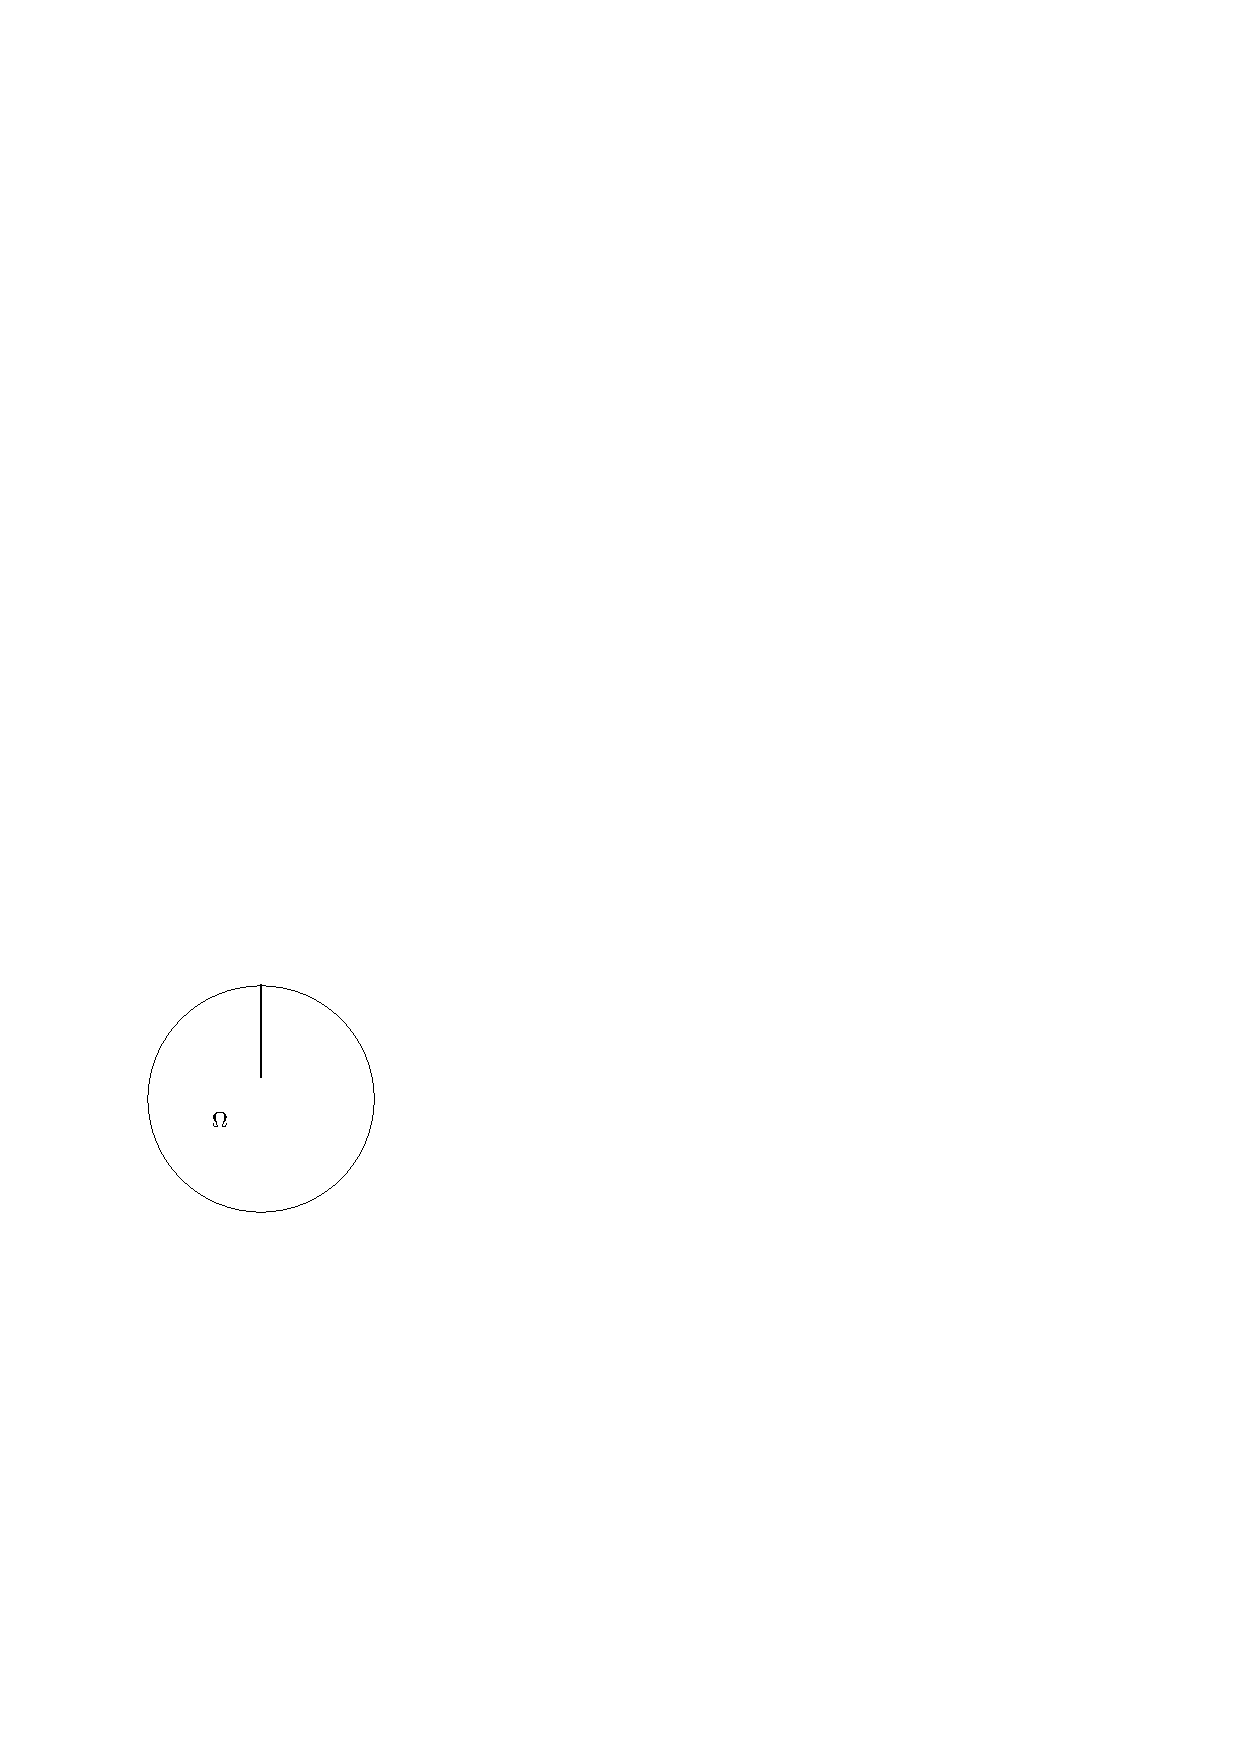
\includegraphics[width=3cm]{figures/slitdomain}\quad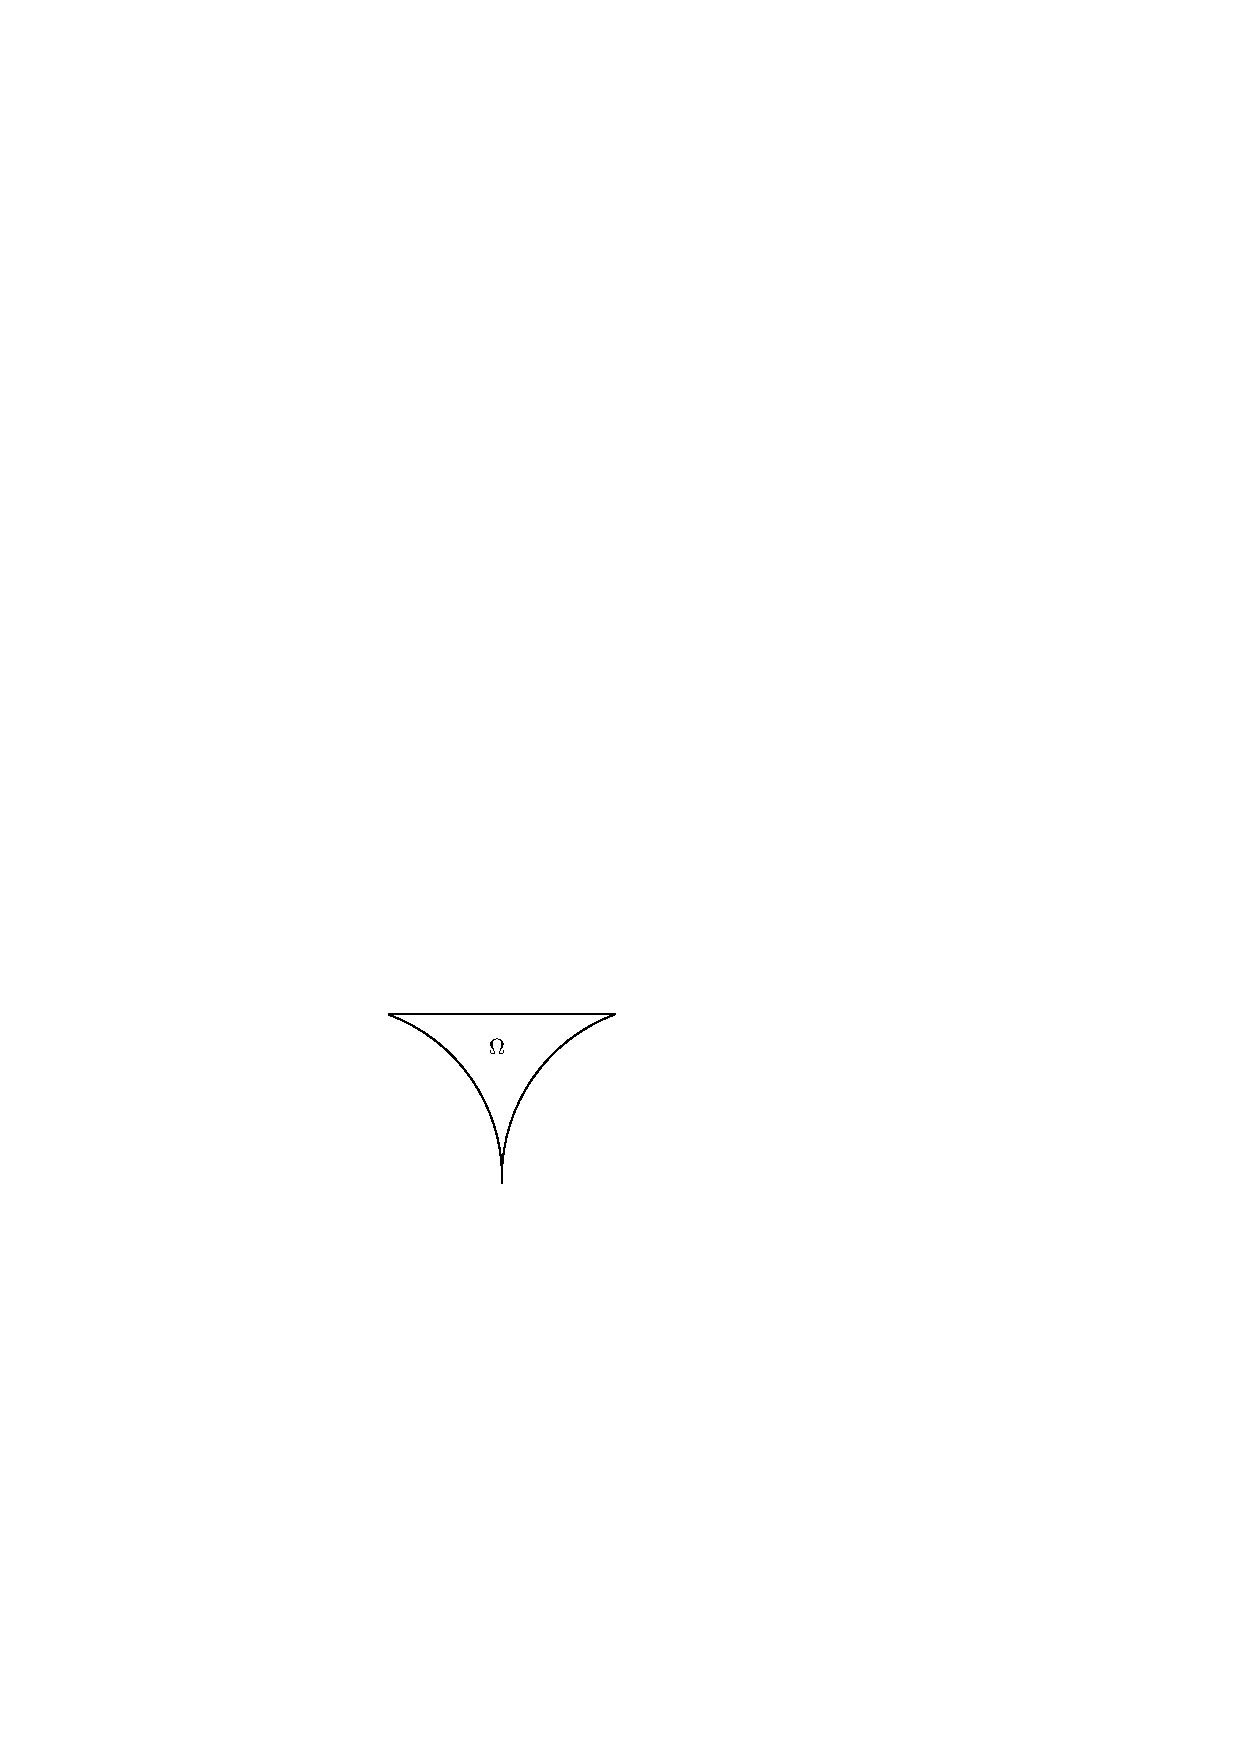
\includegraphics[width=3.5cm]{figures/cuspdomain}\\
  \caption{Domains that are not Lipschitz: slit domain (left) and cusp domain (right)}\label{nonLipschitzDmain}
\end{figure}


Let $\alpha=(\alpha_1, \cdots, \alpha_n)\in\mathbb Z_+^n$, where $\mathbb Z_+^n$ is the set of non-negative integers, be a vector
of nonnegative integers. Denote by $|\alpha|=\sum_{i=1}^n\alpha_i$. For a smooth function $v$ and $x =(x_1,  x_2, \cdots, x_n)\in\mathbb R^n$, denote
\[
D^{\alpha}v=\frac{\partial^{|\alpha|}v}{\partial x_1^{\alpha_1}\cdots\partial x_n^{\alpha_n}},\quad \textrm{and } x^{\alpha}=x_1^{\alpha_1}\cdots x_n^{\alpha_n}.
\]

Several basic Banach spaces will often be used in this book. $C(\bar{\Omega})$ is the space of continuous functions on $\bar{\Omega}$
with the usual maximum norm
\[
\|v\|_{C(\bar{\Omega})}=\max_{x\in\bar{\Omega}}|v(x)|.
\]
$C_0^{\infty}(\Omega)$ denotes the space of infinitely differential functions in $\Omega$
 that vanish in some neighborhood of $\partial\Omega$; namely $\mathrm{supp}(v)\subset\Omega$, where
 \[
 \textrm{supp}(v)=\textrm{closure of }\{x\in\Omega: v(x)\neq0\}.
 \]

A function $u$ that is measurable on $\Omega$ is said to be
\textbf{essentially bounded} on $\Omega$ if there is a constant $K$ such that $|u(x)|\leq K$ a.e. on $\Omega$.
The greatest lower bound of such constants $K$ is called the essential supremum of
$|u|$ on $\Omega$, and is denoted by $\textrm{ess}\sup_{x\in\Omega}|u(x)|$.

Given $1\leq p<\infty$, denote by $L^p(\Omega)$ the class of all measurable functions $u$ defined on
$\Omega$ for which $\int_{\Omega}|u(x)|^p\dx<\infty$, and by $L^{\infty}(\Omega)$ the vector space of all functions $u$ that are essentially bounded on $\Omega$.
The norm is defined by
\[
\|u\|_{p,\Omega}=\left(\int_{\Omega}|u|^p\dx\right)^{1/p}\quad\textrm{for }1\leq p<\infty,
\]
and
\[
\|u\|_{\infty,\Omega}=\textrm{ess}\sup_{x\in\Omega}|u(x)|.
\]

We identify in $L^p(\Omega)$ with $1\leq p\leq\infty$ functions that are equal almost everywhere in $\Omega$; the elements
of $L^p(\Omega)$ are thus equivalence classes of measurable functions satisfying $\|u\|_{p,\Omega}<\infty$, two
functions being equivalent if they are equal a.e. in $\Omega$.

\begin{exe}
Prove that $L^p(\Omega)$, $1\leq p\leq\infty$ defined above are Banach spaces.
\end{exe}


\subsection{Definition of Sobolev spaces}
The conventional way to understand a function is
through its point-wise values which is not adequate. It is better to understand a function as
a functional through its action on a space of unproblematic test functions (convential and
well-behaved functions). In this way, the concept of functions can be generalized to distributions.
``Integration by parts'' is used to extend the differentiation operators from classic
differentiable functions to distributions by shifting the operators to the test functions.
Sobolev spaces will be first defined here for integer orders using the concept of distributions
and their weak derivatives. The fractional order Sobolev spaces will be introduced
by looking at the $p$th power integrable of quotient of difference. Definitions will also be
given to Sobolev spaces satisfying certain zero boundary conditions.

\vskip0.5cm\noindent{\it Distributions and weak derivatives}.
We begin with the nice function space $C_0^{\infty}(\Omega)$. Obviously
$C_0^{\infty}(\Omega)$ is a real vector space and can be turned into a topological vector space
by a proper topology. The space $C_0^{\infty}(\Omega)$ equipped with the following topology is denoted
by $\mathcal D(\Omega)$: a sequence of functions $\{\phi_k\}\subset C_0^{\infty}(\Omega)$ is said to be convergent to a function
$\phi\in C_0^{\infty}(\Omega)$ in the space $\mathcal D(\Omega)$ if
\begin{enumerate}
\item there exists a compact set $K\subset\Omega$
 such that for all $k$, $\textrm{supp}(\phi_k-\phi) \subset K$, and
\item for every $\alpha\in\mathbb Z_+^n$, we have $\lim_{k\to\infty}D^{\alpha}\phi_k(x) = D^{\alpha}\phi(x)$ uniformly on $K$.
\end{enumerate}

The space, denoted by $\mathcal D'(\Omega)$, of all continuous linear functionals on $\mathcal D(\Omega)$ is called the (Schwarz) {\it distribution space}. The space $\mathcal D'(\Omega)$ will be equipped with the weak star
topology. Namely, in $\mathcal D'(\Omega)$, a sequence $T_n$ converge to $T$ in the distribution sense if and only if $\langle T_n, \phi\rangle\to\langle T, \phi\rangle$ for all $\phi\in\mathcal D(\Omega)$, where $\langle\cdot, \cdot\rangle: \mathcal D'(\Omega)\times \mathcal D(\Omega)\to\mathbb R$ is the
duality pair. A function $\phi$ belonging to $\mathcal D(\Omega)$ is called a {\it test function} since the action of a
distribution on $\phi$ can be thought as a test.

\begin{exm}\label{exm:diracdelta}
By the definition, an element in $\mathcal D'(\Omega)$ is uniquely determined by its action.
The action could be very general and abstract as long as it is linear and continuous. As an example, let us introduce the Dirac delta distribution $\delta\in\mathcal D'(\Omega)$ with $0\in\Omega\subset\mathbb R^n$ defined
as
\[
\langle \delta, \phi\rangle = \phi(0) \quad\textrm{ for all } \phi\in \mathcal D(\Omega).
\]
\end{exm}

One important class of distributions is to use the integration as the action. A function
is called {\it locally integrable} if it is Lebesgue integrable over every compact subset of $\Omega$.
We define the space $L^1_{\textrm{loc}}(\Omega)$ as the space containing all locally integrable functions. We
can embed $L^1_{\textrm{loc}}(\Omega)$ into $\mathcal D'(\Omega)$ using the integration as the duality action. For a function
$u\in L^1_{\textrm{loc}}(\Omega)$, define $T_u\in\mathcal D'(\Omega)$ as
\[
\langle T_u, \phi\rangle:=\int_{\Omega}u\phi\dx\quad \textrm{for all }\phi\in\mathcal D(\Omega).
\]
We shall still denoted $T_u$ by $u$. The correspondence $u \mapsto T_u$ is often used to identify an ``ordinary'' function as a distribution.

A distribution is often also known as a {\it generalized function} as the concept of distribution
is a more general than the concept of the classic function. One of the basic distribution
which is not an ``ordinary'' function is the Dirac $\delta$-distribution introduced in Example~\ref{exm:diracdelta}. Indeed, one motivation of the invention of distribution space is to include Dirac delta
``function''.

\begin{exe}
Prove that it is not possible to represent delta distribution by a locally integrable
function.
\end{exe}

If $u$ is a smooth function, it follows from integration by parts that, for any $\alpha\in\mathbb Z_+^n$
\[
\int_{\Omega}D^{\alpha}u(x)\phi(x)\dx=(-1)^{|\alpha|}\int_{\Omega}u(x)D^{\alpha}\phi(x)\dx\quad\textrm{for all } \phi\in\mathcal D(\Omega).
\]
There are no boundary terms, since $\phi$ has compact support in $\Omega$
 and thus $\phi$, together with
its derivatives, vanishes near $\partial\Omega$. The above identity is the basis for defining derivatives
for a distribution. If $T\in\mathcal D'(\Omega)$, then for any $\alpha\in\mathbb Z_+^n$, we define {\it weak derivative} $D^{\alpha}T$ as
the distribution given by
\[
\langle D^{\alpha}T, \phi\rangle=(-1)^{|\alpha|}\langle T, D^{\alpha}\phi\rangle\quad\textrm{for all } \phi\in\mathcal D(\Omega).
\]
It is easy to see for a differentiable function, its weak derivative coincides with its classical
derivative. But in general, the weak derivative is much weaker than the classical one such
that the differential operator can be extended from differential functions to a much larger
space: the space of distributions. For example, we can even talk about the derivative of a
discontinuous function.

\begin{exm}
The Heaviside step function is defined as $S(x) = 1$ for $x > 0$ and $S(x) = 0$
for $x < 0$. By the definition
\[
\int_{\mathbb R}S'\phi\dx=-\int_{\mathbb R}S\phi'\dx=-\int_0^{\infty}\phi'\dx=\phi(0).
\]
Therefore $S'=\delta$ in the distribution sense but \textcolor[rgb]{1.00,0.00,0.00}{$\delta$ is not a function in $L_{\textrm{loc}}^1(\Omega)$}.
\end{exm}

\vskip0.5cm\noindent{\it Integer order Sobolev spaces}.
The Sobolev space of index $(k, p)$, where $k$ is a nonnegative
integer and $p\geq1$, is defined by
\[
W^{k,p}(\Omega):=\{v\in L^p(\Omega): D^{\alpha}v\in L^p(\Omega)\;\textrm{  for all } |\alpha|\leq k\}
\]
with a norm $\|\cdot\|_{k,p,\Omega}$
 given by
\[
\|v\|_{k,p,\Omega}^p:=\sum_{|\alpha|\leq k}\|D^{\alpha}v\|_{0,p,\Omega}^p.
\]
We will have occasions to use the seminorm $|\cdot|_{k,p,\Omega}$
 given by
\[
|v|_{k,p,\Omega}^p:=\sum_{|\alpha|= k}\|D^{\alpha}v\|_{0,p,\Omega}^p.
\]

For $p = 2$, it is customary to write
$H^k(\Omega) := W^{k,2}(\Omega)$, which is a Hilbert space
together with an inner product as follows
\[
(u, v)_{H^k(\Omega)} =\sum_{|\alpha|\leq k}(D^{\alpha}u, D^{\alpha}v)_{L^2(\Omega)}=\sum_{|\alpha|\leq k}\int_{\Omega}D^{\alpha}uD^{\alpha}v\dx
\]
and the corresponding norm is denoted by $\|v\|_{k, \Omega}=\|v\|_{k, 2, \Omega}$.

\begin{exe}
Prove that $W^{k,p}(\Omega)$ is a Banach space.
\end{exe}

For a function in $L^{p}(\Omega)$, treating it as a distribution, its weak derivatives always exists as distributions. But the weak derivative may not be in the space $L^{p}(\Omega)$. Therefore an element in $W^{k,p}(\Omega)$ possesses certain smoothness.

\begin{exm}
We consider the Heaviside function restricted to $(-1, 1)$ and still denote
by $S$. The weak derivative of $S$ is Delta distribution which is not integrable. Therefore $S \notin H^1(-1, 1)$.
\end{exm}

\begin{exm}
Let $u(x)=|x|$ for $x\in(-1,1)$ be an anti-derivative of $2(S-1/2)$. Obviously
$u\in L^2(-1, 1)$ and $u'\in L^2(-1, 1)$. Therefore $u\in H^1(-1, 1)$.
\end{exm}


\vskip0.5cm\noindent{\it Fractional order Sobolev spaces}.
In the definition of classic derivatives, it takes the pointwise
limit of the quotient of difference. For functions in Sobolev space, we shall use the
$p$th power integrability of the quotient difference to characterize the differentiability.

For $0<\theta<1$ and $1\leq p<\infty$, we define
\[
W^{\theta, p}(\Omega)=\left\{v\in L^p(\Omega): \int_{\Omega}\int_{\Omega}\frac{|v(x)-v(y)|^p}{|x-y|^{n+\theta p}}\dx\dd y<\infty\right\}
\]
and
\[
H^{\theta}=W^{\theta, 2}(\Omega).
\]
In $W^{\theta, p}(\Omega)$, we define the following semi-norm
\begin{equation}\label{eq:fsobolevseminorm}
|v|_{\theta,p,\Omega}:=\left(\int_{\Omega}\int_{\Omega}\frac{|v(x)-v(y)|^p}{|x-y|^{n+\theta p}}\dx\dd y\right)^{1/p},
\end{equation}
and norm
\[
\|v\|_{\theta,p,\Omega}:=\left(\|v\|_{0,p,\Omega}^p+|v|_{\theta,p,\Omega}^p\right)^{1/p}.
\]

\begin{exm}
For the Heaviside function S restricted to $(-1, 1)$, we look at the integral \eqref{eq:fsobolevseminorm}. To be in the space $W^{\theta, p}(\Omega)$, it is essential
to have the integral
\[
\int_0^1\frac{1}{x^{\theta p}}\dx<\infty.
\]
That is to require $\theta < 1/p$. In particular, we conclude $S\in H^{1/2-\epsilon}(-1, 1)$ for any $0 <\epsilon\leq 1/2$ but $S\notin H^{1/2}(-1, 1)$.
\end{exm}

Given $s = k + \theta$ with a real number $\theta\in(0, 1)$ and an integer $k\geq0$, define
\[
W^{s,p}(\Omega):=\{v\in W^{k,p}(\Omega): D^{\alpha}v\in W^{\theta,p}(\Omega), |\alpha|= k\}.
\]
In $W^{s,p}(\Omega)$, we define the following semi-norm and norm
\[
|v|_{s,p,\Omega}=\left(\sum_{|\alpha|=k}|D^{\alpha}v|_{\theta,p,\Omega}^p\right)^{1/p}, \quad \|v\|_{s,p,\Omega}=\left(\|v\|_{k,p,\Omega}^p+|v|_{s,p,\Omega}^p\right)^{1/p}.
\]


\vskip0.5cm\noindent{\it Negative order Sobolev spaces}.
$W^{k,p}(\Omega)$ is a Banach space, i.e., it is complete in the
topology induced by the norm $\|\cdot\|_{k,p,\Omega}$. Indeed
$\{\phi\in C^{\infty}(\Omega): \|\phi\|_{k,p,\Omega}<\infty\}$ is dense in
$W^{k,p}(\Omega)$. When $\Omega$ satisfies the segment condition, $C^{\infty}(\overline{\Omega})$ is dense in
$W^{k,p}(\Omega)$ \cite{AdamsFournier2003}.
 The closure of
$C_0^{\infty}(\Omega)$ with respect to the same topology is denoted
by $W_0^{k,p}(\Omega)$. For $p = 2$, we usually write $H_0^k(\Omega) = W_0^{k,2}(\Omega)$. Roughly speaking for $u\in H_0^1(\Omega)$, $u|_{\partial \Omega}=0$ in an appropriate sense. Except $k = 0$ or
$\Omega=\mathbb R^n$, $W_0^{k,p}(\Omega)$ is a
proper subspace of $W^{k,p}(\Omega)$.

For $k\in\mathbb N$, $W^{-k,p}(\Omega)$ is defined as the dual space of $W_0^{k,p'}(\Omega)$, where $p'$ is the conjugate
of $p$, i.e., $1/p + 1/p' = 1$. In particular $H^{-k}(\Omega) = (H_0^{k}(\Omega))'$, and for $f\in H^{-k}(\Omega)$
\[
\|f\|_{-k,\Omega}=\sup_{v\in H_0^k(\Omega)}\frac{\langle f, v\rangle}{\|v\|_{k,\Omega}}.
\]

%\begin{theorem}[refs?]
%Let $v\in\mathcal D'(\Omega)$. Then $v\in W^{-k,p}(\Omega)$ if and only if
%\[
%v=\sum_{|\alpha|\leq k}D^{\alpha}v_{\alpha}\quad\textrm{for some } v_{\alpha}\in L^p(\Omega).
%\]
%\end{theorem}


\subsection{Extension theorems}
The extension theorem presented below is a fundamental result
for Sobolev spaces. Fourier transform is a powerful tool. But unfortunately it only works
for functions defined in the entire space $\mathbb R^n$. To generalize results proved on the whole $\mathbb R^n$ to a bounded domain $\Omega$, we can try to extend the function defined in $W^{k,p}(\Omega)$ to
$W^{k,p}(\mathbb R^n)$. The extension of a function $u\in L^p(\Omega)$ is trivial. For example, we can simply
set $u(x) = 0$ when $x\notin\Omega$ which is called zero extension. But such extension will create
a bad discontinuity along the boundary and thus cannot control the norm of derivatives
especially the boundary is non-smooth. The extension of Sobolev space $W^{k,p}(\Omega)$ is subtle.
We only present the result here.

\begin{theorem}\label{thm:sobolevextension}
For any bounded Lipschitz domain $\Omega$, for any $s\geq0$ and $1\leq p \leq \infty$,
there exits a linear operator $E : W^{s,p}(\Omega)\to W^{s,p}(\mathbb R^n)$ such that
\begin{enumerate}
\item $Eu|_{\Omega}= u$, and
\item $E$ is continuous. Namely there exists a constant $C(s, \Omega)$ which is increasing with respect to $s\geq0$ such that, for all $1\leq p \leq \infty$,
\[
\|Ev\|_{s,p,\mathbb R^n}\leq C(s,\Omega)\|v\|_{s,p,\Omega}\quad\textrm{for all }v\in W^{s,p}(\Omega).
\]
\end{enumerate}
\end{theorem}

Theorem \ref{thm:sobolevextension} is well-known for integer order Sobolev spaces defined on smooth domains
and the corresonding proof can be found in most text books on Sobolev spaces. But
for Lipschitz domains and especially for fractional order spaces Theorem \ref{thm:sobolevextension} is less well-known
and the the proof of the theorem for these cases is quite complicated. For integer
order Sobolev spaces on Lipschitz domains, we refer to Calder\'on \cite{Calderon1961} or Stein \cite{Stein1970}. For
factional order Sobolev spaces on Lipschitz domains, we refer to the book by McLean \cite{McLean2000}.


\subsection{Embedding theorems}
Embedding theorems of Sobolev spaces are what make the
Sobolev spaces interesting and important. The Sobolev spaces $W^{k,p}(\Omega)$ are defined using
weak derivatives. The smoothness using weak derivatives is weaker than that using classic
derivatives.

\begin{exm}\label{example:20180304-1}
In two dimensions, consider the function $u(x) = \ln|\ln|x||$ when $|x| <1/e$ and $u(x) = 0$ when $|x| \geq 1/e$. It is easy to verify that $u\in H^1(\mathbb R^2)$. But $u$ is unbounded, i.e., $u\notin C(\mathbb R^2)$.
\end{exm}

Sobolev embedding theorem connects ideas of smoothness using ``weak'' and ``classic''
derivatives. Roughly speaking, it says that if a function is weakly smooth enough, then it
implies certain classic smoothness with less order of smoothness.

\begin{exe}\label{exercise:20180304-1}
Prove that if $u\in W^{1,1}(0, 1)$, then $u \in L^{\infty}(0, 1)$.
\end{exe}

We now present the general embedding theorem. For two Banach spaces $B_1$ and $B_0$, we
say $B_1$ is continuously embedded into $B_0$, denoted by $B_1\hookrightarrow B_0$, if for any $u\in B_1$, it is also in $B_0$ and the embedding map is continuous, i.e., for all $u\in B_1$
\[
\|u\|_{B_0}\lesssim \|u\|_{B_1}.
\]

\begin{theorem}[General Sobolev embedding]
Let $1\leq p\leq \infty$, $k\in\mathbb Z_+$ and $\Omega$ be a
bounded Lipschitz domain in $\mathbb R^n$.


\noindent Case 1. $kp>n$
\[
W^{k,p}(\Omega)\hookrightarrow C(\bar{\Omega}).
\]

\noindent Case 2. $kp=n$
\[
W^{k,p}(\Omega)\hookrightarrow L^q(\Omega)\quad \textrm{for all } q\in[1,\infty).
\]

\quad\;\, Furthermore
\[
W^{n,1}(\Omega)\hookrightarrow C(\bar{\Omega}).
\]

\noindent Case 3. $kp<n$
\[
W^{k,p}(\Omega)\hookrightarrow L^q(\Omega)\quad \textrm{with } \frac{1}{q}=\frac{1}{p}-\frac{k}{n}.
\]
\end{theorem}

We take the following visualization of Sobolev spaces from DeVore \cite[page 93]{DeVore1998}. This
will give us a simple way to keep track of various results. We shall do this by using points
in the upper right quadrant of the plane. The $x$-axis will correspond to the $L^p$ spaces
except that $L^p$ is identified with $x = 1/p$ not with $x = p$. The $y$-axis will correspond
to the order of smoothness. For example, the point $(1/p, k)$ represents the Sobolve space
$W^{k,p}(\Omega)$. The line with slope $n$ (the dimension of Euclidean spaces) passing through
$(1/p, 0)$ is the demarcation line for embeddings of Sobolev spaces into $L^p(\Omega)$ (see Figure~\ref{fig:sobolevEmbeddingLine}). Any Sobolev space with indices corresponding to a point above that line is embedded
into $L^p(\Omega)$ and space below that line cannot be embedded into $L^p(\Omega)$.
\begin{figure}[htbp]
  \centering
  % Requires \usepackage{graphicx}
  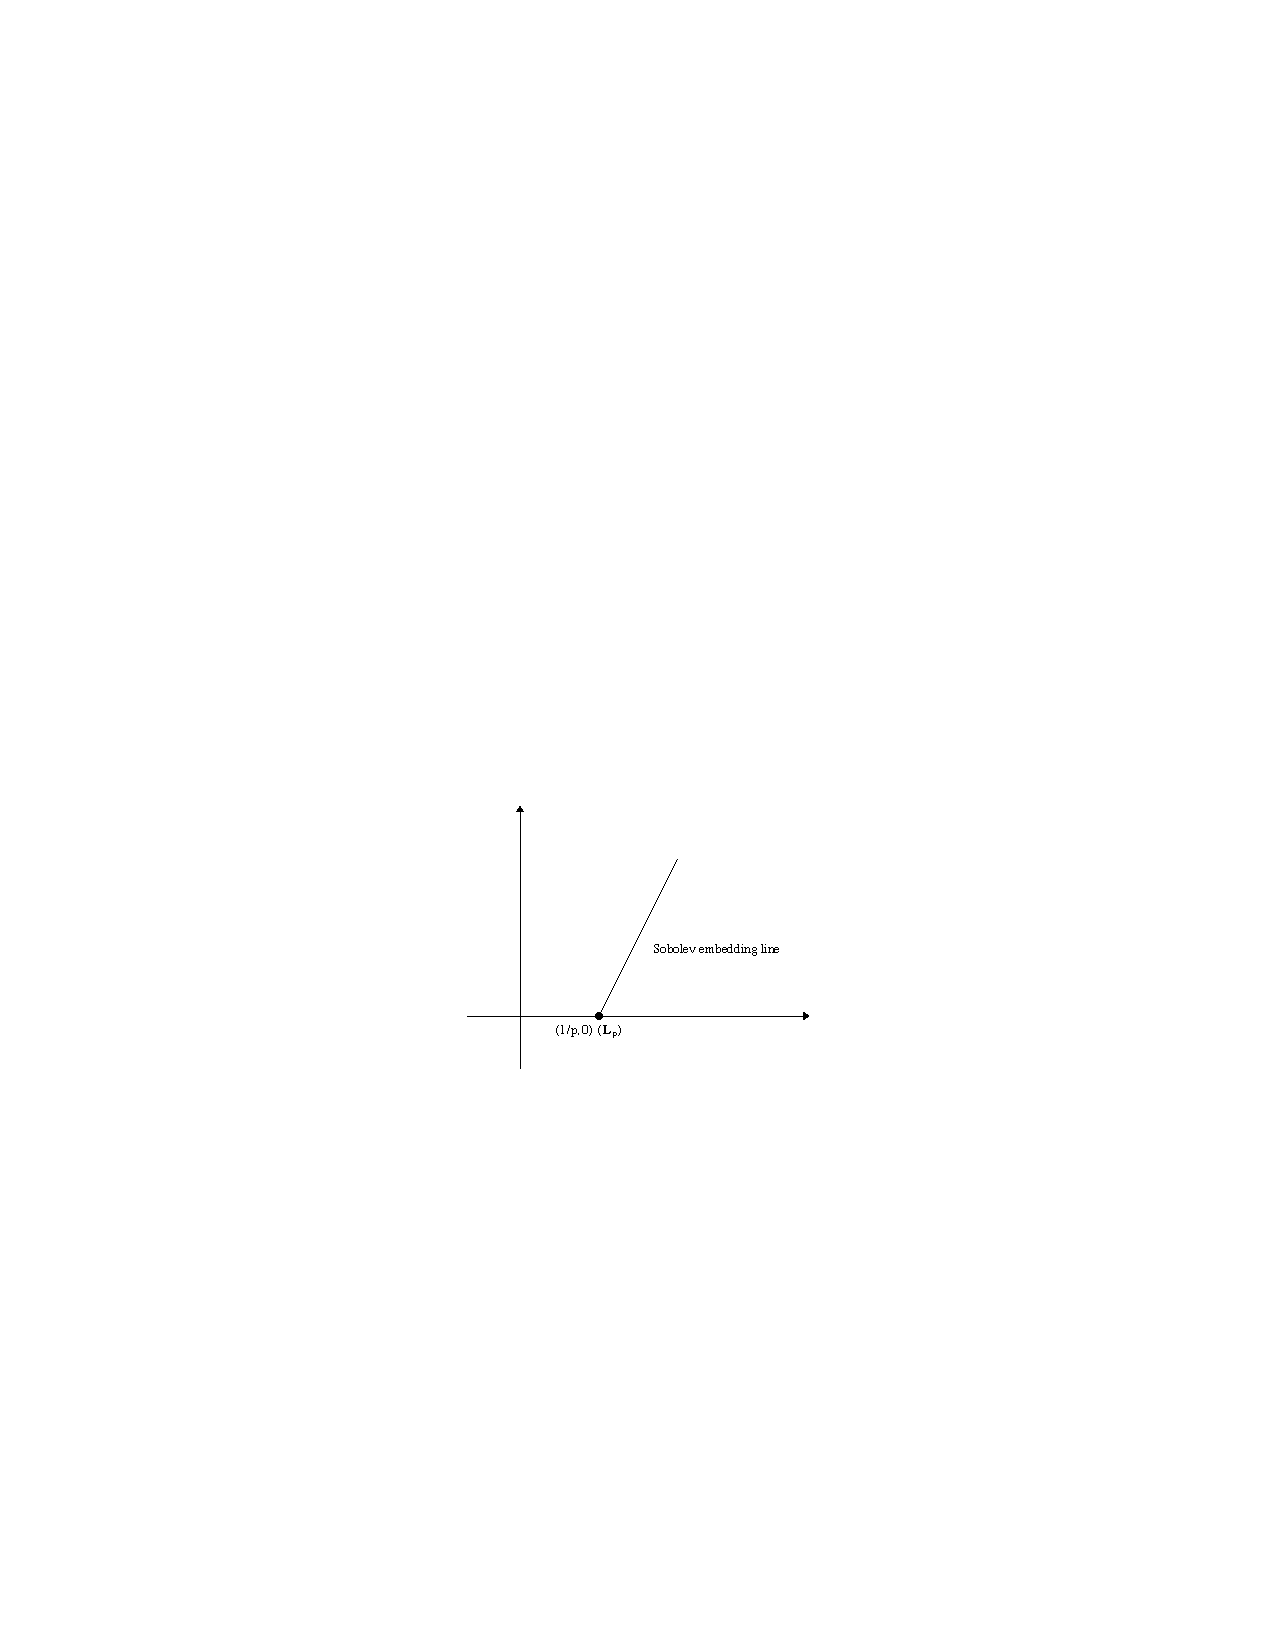
\includegraphics[width=7cm]{figures/sobolevEmbeddingLine}\\
  \caption{Sobolev embedding line}\label{fig:sobolevEmbeddingLine}
\end{figure}

To be quickly determine if a point lies above the demarcation line or not, we introduce
the {\it Sobolev number}
\[
\textrm{sob}_n(k, p)=k-\frac{n}{p}.
\]
If $\textrm{sob}_n(k, p) > 0$, functions from $W^{k,p}(\Omega)$ are continuous (or more precisely can find a
continuous representative in its equivalent class). In general
\[
W^{k,p}(\Omega)\hookrightarrow W^{l,q}(\Omega)\quad\textrm{if } k>l \textrm{ and } \textrm{sob}_n(k, p)>\textrm{sob}_n(l, q).
\]
Sobolev spaces corresponding to points on the demarcation line may or may not be
embedded in $L^p(\Omega)$. For example, for $n\geq1$
\[
W^{n,1}(\Omega)\hookrightarrow L^{\infty}(\Omega)\quad \textrm{but } W^{1,n}(\Omega)\not\hookrightarrow L^{\infty}(\Omega).
\]
Note that $W^{1,n}(\Omega)\hookrightarrow L^{p}(\Omega)$ for all $1\leq p < \infty$. Furthermore there exists a constant
$C(n, \Omega)$ depending on the dimension of Euclidean space and the Lipschitz domain such
that
\begin{equation*}
\|v\|_{0,p,\Omega}\leq C(n, \Omega)p^{1-1/n} \|v\|_{1,n,\Omega}\quad\textrm{for all }1\leq p < \infty.
\end{equation*}

\begin{exm}
By the emebedding theorem, we have
\begin{enumerate}
\item $H^1(\Omega)\hookrightarrow C(\bar{\Omega})$ in one dimension (Exercise~\ref{exercise:20180304-1}).
\item $H^1(\Omega)\not\hookrightarrow C(\bar{\Omega})$ for $n\geq2$ (Example~\ref{example:20180304-1}).
Namely there is no continuous representation of a function in $H^1(\Omega)$ for $n\geq2$ and thus its point-wise value is
not well defined.
\item In 2-D, $H^1(\Omega)\hookrightarrow L^p(\Omega)$ for any $1\leq p<\infty$; in 3-D, $H^1(\Omega)\hookrightarrow L^p(\Omega)$ for any $1\leq p\leq6$.
\end{enumerate}
\end{exm}


\subsection{Trace Theorem}
The trace theorem is to define function values on the boundary. If
$u\in C(\bar{\Omega})$, then $u(x)$ is well defined for $x\in\partial\Omega$. But for $u\in W^{k,p}(\Omega)$, the function
is indeed defined as an equivalent class of Lebesgue integrable functions, i.e., $u \sim v$ if
and only if $u = v$ almost everywhere. The boundary $\partial\Omega$ is a measure zero set (in $n$th
dimensional Lebesgue measure) and thus the pointwise value of $u|_{\partial\Omega}$ is not well defined
for functions in Sobolev spaces.

\begin{theorem}
Let $\Omega\subset\mathbb R^n$ be a bounded domain with smooth or Lipschitz boundary
$\Gamma=\partial\Omega$. Then the trace operator $\gamma: C^1(\bar{\Omega})\to C(\Gamma)$
 can be continuously extended to
$\gamma: H^1(\Omega)\to H^{1/2}(\Gamma)$, i.e., the trace inequality holds:
\[
\|\gamma(u)\|_{1/2, \Gamma}\lesssim \|u\|_{1, \Omega}\quad \textrm{for all } u\in H^1(\Omega).
\]
Furthermore the trace operator is surjective and has a continuous right inverse.
\end{theorem}

More general, if $\Omega$ is a Lipschitz domain, then the trace operator
$\gamma: H^s(\Omega)\to H^{s-1/2}(\Gamma)$ is bounded for $1/2 < s < 3/2$. See McLean \cite[pages 100-106]{McLean2000}.


\begin{theorem}
Suppose that $\Omega\subset\mathbb R^n$ has a Lipschitz boundary, and that $p$ is a real number in the range $1\leq p\leq \infty$. Then there is a constant $C$ such that
\[
\|v\|_{0, p,\partial\Omega}\leq C\|v\|_{0,p,\Omega}^{1-1/p}\|v\|_{1,p,\Omega}^{1/p}\quad\forall~v\in W^{1,p}(\Omega).
\]
\end{theorem}




\subsection{Norm Equivalence Theorem}
The definition of norm $\|\cdot\|_{k+1,p}$ involves all the $i$th
derivatives for $i\leq k + 1$. But the highest one is the critical one. That is we can prove \cite[Theorem 5.2 in page 135]{AdamsFournier2003}
\[
\|u\|_{k+1,p}\eqsim\|u\|_{0,p}+|u|_{k+1,p}\quad\textrm{for all } u\in W^{k+1, p}(\Omega).
\]

\begin{theorem}[Sobolev norm equivalence]
Let $P_k(\Omega)$($k\geq0$) be the set of all polynomials in $\Omega$ with the total degree no more than $k$. Let $N=\mathrm{dim}P_k(\Omega)$. Assume $f_i\in(W^{k+1,p}(\Omega))'$, $i=1,2,\cdots,N$, $p\in[1,\infty]$ such that for $q\in P_k(\Omega)$, $q=0$ if $f_i(q)=0$ for all $1\leq i\leq N$. Then
\begin{equation}\label{eq:sobolevnormequiv}
\|v\|_{k+1,p,\Omega}\lesssim  |v|_{k+1,p,\Omega}+\sum_{i=1}^N|f_i(v)|\quad\textrm{for all } v\in W^{k+1,p}(\Omega).
\end{equation}
\end{theorem}

As a special case of the Sobolev norm equivalence theorem, we present the following
variants of Poincar\'e or Friedrichs inequalities. Assume that $\Gamma$ is a measurable subset of
$\Omega$ with positive measure (in $n-1$ dimensional Lebesgue measure). Choosing $f_0(v) =\int_{\Gamma}v\dd s$
 in \eqref{eq:sobolevnormequiv}, we obtain the Friedrichs inequality
\[
\|v\|_{1,p,\Omega}\lesssim  |v|_{1,p,\Omega}+\left|\int_{\Gamma}v\dd s\right|\quad\textrm{for all } v\in W^{1,p}(\Omega).
\]
Consequently, we have the Poincar\'e inequality
\begin{equation}\label{eq:poincareinequalityW1p}
\|v\|_{1,p,\Omega}\lesssim  |v|_{1,p,\Omega}\quad\textrm{for all } v\in W_0^{1,p}(\Omega).
\end{equation}
Choosing $f_0(v)=\int_{\Omega}v\dx$, we obtain the Poincar\'e-Friedrichs inequality
\[
\|v\|_{1,p,\Omega}\lesssim  |v|_{1,p,\Omega}+\left|\int_{\Omega}v\dx\right|\quad\textrm{for all } v\in W^{1,p}(\Omega).
\]
Consequently, let $\bar{v} =\int_{\Omega}v\dx/|\Omega|$ denote the average of $v$ over $\Omega$, we get the averaged
Poincar\'e inequality
\[
\|v-\bar{v}\|_{1,p,\Omega}\lesssim  |v|_{1,p,\Omega}\quad\textrm{for all } v\in W^{1,p}(\Omega).
\]

\begin{theorem}\label{thm:quotientspacenorms}
Let $k\geq0$ and $p\in[1, \infty]$. Then
\[
\inf_{q\in P_k(\Omega)}\|v+q\|_{k+1,p,\Omega}\lesssim  |v|_{k+1,p,\Omega}\quad\textrm{for all } v\in W^{k+1,p}(\Omega),
\]
\[
\|\dot{v}\|_{k+1,p,\Omega}\lesssim  |\dot{v}|_{k+1,p,\Omega}\quad\textrm{for all } v\in W^{k+1,p}(\Omega)/P_k(\Omega).
\]
\end{theorem}


All constants hidden in the notation $\lesssim$ depends on the size and shape of the domain
$\Omega$. This is important when apply them to one simplex with diameter $h$ in finite element
methods.

\subsection{Green's formulas}
Let $\nu=(\nu_1, \nu_2, \cdots, \nu_n)$ be the unit outward normal to $\partial\Omega$.
The (outer) normal derivative operator
\[
\partial_{\nu}=\sum_{i=1}^n\nu_i\partial_i
\]
is defined almost everywhere along $\partial\Omega$ for smooth functions.
Given two functions $u, v\in H^1(\Omega)$, the following fundamental Green's formula
\[
\int_{\Omega}u\partial_iv\dx=-\int_{\Omega}\partial_iuv\dx+\int_{\partial\Omega}uv\nu_i\dd s
\]
holds for any $i=1, \cdots, n$.
From this formula, other Green's formulas may be easily deduced.
For example, replacing $u$ by $\partial_iu$ and taking the sum from $1$ to $n$, we get
\[
\int_{\Omega}\sum_{i=1}^n\partial_iu\partial_iv\dx=-\int_{\Omega}\Delta uv\dx+\int_{\partial\Omega}\partial_{\nu}uv\dd s
\]
for all $u\in H^2(\Omega)$ and $v\in H^1(\Omega)$. As a consequence, we obtain by subtraction
\[
\int_{\Omega}(u\Delta v-\Delta uv)\dx=\int_{\partial\Omega}(u\partial_{\nu}v-\partial_{\nu}uv)\dd s
\]
for all $u\in H^2(\Omega)$ and $v\in H^2(\Omega)$.


\begin{theorem}
Let $m$ be a positive integer. Let $\Omega$, $\Omega_1$ and $\Omega_2$ be three open and bounded domains in $\mathbb R^n$. Suppose
$\bar{\Omega}=\bar{\Omega}_1\cup \bar{\Omega}_2$ and $\Omega_1\cap \Omega_2=\varnothing$. Let $u$ be a function defined in
$\Omega$ such that $u|_{\Omega_1}\in C^{m-1}(\bar{\Omega}_1)\cap H^m(\Omega_1)$ and $u|_{\Omega_2}\in C^{m-1}(\bar{\Omega}_2)\cap H^m(\Omega_2)$.
Then $u\in H^m(\Omega)$ if and only if $u\in C^{m-1}(\bar{\Omega})$.
\end{theorem}
For a piecewise smooth function which is also in $H^1(\Omega)$, then it is globally continuous.
\begin{exe}
Let $\Omega$, $\Omega_1$ and $\Omega_2$ are three open and bounded domains in $\mathbb R^n$. Suppose
$\bar{\Omega}=\bar{\Omega}_1\cup \bar{\Omega}_2$ and $\Omega_1\cap \Omega_2=\varnothing$. Let $u$ be a function defined in
$\Omega$ such that $u|_{\Omega_1}\in C(\bar{\Omega}_1)\cap H^1(\Omega_1)$ and $u|_{\Omega_2}\in C(\bar{\Omega}_2)\cap H^1(\Omega_2)$.
Prove that $u\in H^1(\Omega)$ if and only if $u\in C(\bar{\Omega})$.
\end{exe}



\section{Elliptic Boundary Value Problems and Regularity}

\subsection{Weak formulation}
Let us take the Poisson equation with homogenous Dirichlet
boundary condition
\begin{equation}\label{eq:poisson}
-\Delta u=f\;\; \textrm{in }\Omega, \quad \textrm{and } u|_{\partial\Omega}=0,
\end{equation}
as an example to illustrate the main idea. If there exists a function $u\in C_0^2(\Omega)$
satisfying the Poisson equation, we call $u$ a {\it classic solution}. The smoothness of $u$ excludes
many interesting solutions for physical problems. We need to seek a weak solution in more
broader spaces: Sobolev spaces. Here ``weak'' means the smoothness is imposed by weak
derivatives.

Recall the basic idea of Sobolev space is to treat function as functional. Let us try to
understand the equation \eqref{eq:poisson} in the distribution sense. We seek a solution $u\in \mathcal D'(\Omega)$ such
that for any $\phi\in C_0^{\infty}(\Omega)$,
\[
\langle-\nabla\cdot\nabla u,\phi\rangle:=\langle\nabla u,\nabla\phi\rangle=\langle f, \phi\rangle,
\]
which suggests a weak formulation: find $u\in H_0^1(\Omega)$ such that
\begin{equation}\label{eq:poissonweak}
\int_{\Omega}\nabla u\cdot\nabla v\dx=\int_{\Omega}f v\dx\quad\textrm{for all } v\in H_0^1(\Omega).
\end{equation}
And we can take $f\in H^{-1}(\Omega):=(H_0^1(\Omega))'$.

A generalization of weak formulation \eqref{eq:poissonweak} is: given an $f\in V'$ and a continuous bilinear form $a(\cdot, \cdot): U\times V\to \mathbb R$,  find a solution $u\in U$ such that
\begin{equation*}
a(u, v)=\langle f, v\rangle\quad\textrm{for all } v\in V.
\end{equation*}
Here the space $U$ is the one we seek a solution and thus called {\it trial space}, and $V$ is still
called {\it test space}.


\subsection{Regularity theory}

The weak solution $u$ of \eqref{eq:poissonweak} can be proved to be a solution of \eqref{eq:poisson} in a
more classic sense if $u$ is smooth enough such that we can integration by parts back. The
theory for proving the smoothness of the weak solution is called {\it regularity} theory, which
is the bridge to connect classical and weak solutions.

First we assume right hand side $f\in L^2(\Omega)$ which will imply $\Delta u\in L^2(\Omega)$.
\begin{theorem}
Let $u$ be the solution of \eqref{eq:poissonweak}. If $f\in L^2(\Omega)$, then $-\Delta u = f$ in $L^2(\Omega)$, i.e.
\begin{equation}\label{eq:equilibriumweak}
\int_{\Omega}-\Delta u \,v\dx=\int_{\Omega}fv\dx\quad\forall~v\in L^2(\Omega).
\end{equation}
Furthermore $u = 0$ on $\partial\Omega$ in the trace sense.
\end{theorem}
\begin{proof}
When $f\in L^2(\Omega)$, $\langle f, v\rangle = (f, v)$. Choosing $v\in C_0^{\infty}(\Omega)\subset H_0^1(\Omega)$ in \eqref{eq:poissonweak} implies that
\[
\langle-\Delta u, v\rangle = (f, v)\quad\forall~v\in C_0^{\infty}(\Omega).
\]
That is $-\Delta u$ as a distribution is equal to $f\in L^2(\Omega)$. Since $C_0^{\infty}(\Omega)$ is dense in $L^2(\Omega)$ and
both sides are continuous in $L^2$ topology, we conclude \eqref{eq:equilibriumweak}.
\end{proof}

\begin{theorem}[\cite{Evans2010}]\label{thm:poissonregularitysmooth}
Let $\Omega$ be a smooth and bounded domain of $\mathbb R^n$. Then for each $f \in L^2(\Omega)$,
there exists a unique $u\in H^2(\Omega)$, the solution of \eqref{eq:poissonweak}, that satisfies
\[
\|u\|_{2,\Omega}\leq C\|f\|_{0,\Omega}
\]
where $C$ is a positive constant depending on $\Omega$.
\end{theorem}

Theorem~\ref{thm:poissonregularitysmooth}, however, does not hold on general Lipschitz domains.
The requirement of $\Omega$ is necessary. When $\partial\Omega$ is only Lipschitz continuous, we may not
be able to glue boundary pieces on the corner points. This is not only a technical difficulty.
We now give an example in which the regularity of $u$ depends on the shape of $\Omega$.
\begin{exm}
Let us give a simple counter example. Given $\beta\in (0, 1)$, consider the
following nonconvex domain
\[
\Omega=\{(r, \theta): 0<r<1, 0<\theta<\pi/\beta\}.
\]
Let $v = r^{\beta}\sin(\beta\theta)$. Being the imaginary part of the complex analytic function $z^{\beta}$, $v$ is
harmonic in $\Omega$. Define $u = (1-r^2)v$. A direct calculation shows that
\[
-\Delta u=4(1+\beta)v\quad\textrm{  in }\Omega,\quad\textrm{and } u|_{\partial\Omega}=0.
\]
Note that $4(1+\beta)v\in L^{\infty}(\Omega)\subset L^2(\Omega)$, but $u\notin H^2(\Omega)$.
\end{exm}

Nevertheless, a slightly weaker result does hold for general Lipschitz domains.
\begin{theorem}[\cite{Dauge1988,BacutaBrambleXu2003}]
Assume that $\Omega$ is a bounded Lipschitz domain. Then there exists a constant
$\alpha\in(0, 1]$ such that
\[
\|u\|_{1+\alpha,\Omega}\leq C\|f\|_{\alpha-1,\Omega}
\]
for the solution $u$ of \eqref{eq:poissonweak},
where $C$ is a constant depending on the domain $\Omega$.
\end{theorem}

A remarkable fact is that we can take $\alpha = 1$ in the above theorem for
convex domains. This means that Theorem~\ref{thm:poissonregularitysmooth} can be extended to convex domains.
\begin{theorem}\label{thm:poissonregularityconvex}
Let $\Omega$ be a convex, bounded domain of $\mathbb R^n$. Then for each $f \in L^2(\Omega)$,
there exists a unique $u\in H^2(\Omega)$, the solution of \eqref{eq:poissonweak}, that satisfies
\[
\|u\|_{2,\Omega}\leq C\|f\|_{0,\Omega}
\]
where $C$ is a positive constant depending on $\Omega$.
\end{theorem}

When $\Omega$ is a concave polygon in $\mathbb R^2$, we do not have full regularity, i.e.,
$\alpha < 1$. There are at least two ways to obtain analogous (but weaker) results for concave
domain. The first one (see \cite{Dauge1988,BacutaBrambleXu2003}) is to use fractional Sobolev spaces: namely $-\Delta$:
$H_0^1(\Omega)\cap H^{1+s}(\Omega)\to H^{-1+s}(\Omega)$ which holds for any $s\in [0, s_0)$ for some $s_0\in (0, 1]$
depending on $\Omega$.

Another approach is to use $L^p$ space, instead of $L^2$. It can be shown that (cf. \cite{Grisvard1985})
\[
-\Delta: H_0^1(\Omega)\cap W^{2,p}(\Omega)\to L^{p}(\Omega)
\]
is an isomorphism, which holds for any $p\in(1, p_0)$ for some $p_0 > 1$ that depends on the domain $\Omega$.

% !TEX root = lecture.tex
\chapter{微分复形在偏微分方程中的应用}


\section{Stokes Complex 及应用}
Complex 1.
\begin{equation}\label{CA10}
	\resizebox{0.8\hsize}{!}{$
		\begin{array}{c}
			\xymatrix{	
\mathbb{R} \ar[r] & H_0^1(\Omega)\ar[r]^-{\grad} & \boldsymbol{H}_0(\curl, \Omega)  \ar[r]^-{\curl}
				& \boldsymbol{H}_0(\div, \Omega)    \ar[r]^-{\div} & L_0^2(\Omega) \ar[r]^{} & 0 ,
 }
		\end{array}
		$}
	\end{equation}

Example 1:The Possion equation
\begin{equation}\label{Cw1}
\left\{
\begin{aligned}
-\Delta u &=f,\quad \mathrm{in}\,\Omega \\
 u &=0, \quad \mathrm{on}\,\partial\Omega .
\end{aligned}\right.
\end{equation}
引入新变量
\begin{equation}\label{Cq}
\left\{
\begin{aligned}
\boldsymbol{\sigma} &=\nabla u \\
\div\boldsymbol{\sigma} &=-f.
\end{aligned}\right.
\end{equation}
则方程 (\ref{Cw1})
变为
\begin{equation}\label{Cw2}
\left\{
\begin{aligned}
\div\boldsymbol{\sigma}+f &=0,\quad \mathrm{in}\,\Omega\\
\boldsymbol{\sigma} -\nabla u&=0,\quad \mathrm{in}\,\Omega\\
 u &=0, \quad \mathrm{on}\,\partial\Omega.
\end{aligned}\right.
\end{equation}
在结合复形(\ref{CA10})的后半部分, 则方程 (\ref{Cw2})的变分形式为: $\boldsymbol{\tau}\in\boldsymbol{H}_0(\div, \Omega),\,u\in L_0^{2}(\Omega)$, 使得
\begin{equation}\label{Cp1}
\left\{
\begin{aligned}
(\boldsymbol{\sigma},\boldsymbol{\tau})+(\div\boldsymbol{\tau},u)&=0
  &&\forall \,\, \boldsymbol{\tau}\in \boldsymbol{H}_0(\div, \Omega),
 \\
 ( \div\boldsymbol{\sigma},v) &=0 &&\forall \,\, v\in L_0^{2}(\Omega),
\end{aligned}\right.
\end{equation}
下面利用复形(\ref{CA10})来证明 inf-sup 条件和强制性 .\\
(1) inf-sup 条件: 对 $v\in L_0^{2}(\Omega)$, 根据复形(\ref{CA10})可知 $ \exists\,\boldsymbol{\tau}\in \boldsymbol{H}_0(\div, \Omega)$,
使得
$\div\boldsymbol{\tau}=v$, 则有
\begin{align*}
\|v\|_{ 0} =\frac{(\div\boldsymbol{\tau},v)}{\|\div\boldsymbol{\tau}\|_{0}}
\lesssim\sup_{\boldsymbol{\tau}\in\boldsymbol{H}_0(\div, \Omega)}\frac{(\div\boldsymbol{\tau},u)}{\|\boldsymbol{\tau}\|_{\boldsymbol{H}(\div)}}
\end{align*}
(2) 强制性
\begin{align*}
\ker \boldsymbol{B}
&=\{\boldsymbol{\tau}\in \boldsymbol{H}_0(\div, \Omega),\,(\div\boldsymbol{\tau},v)=0,\quad\forall \, v\in L_0^{2}(\Omega)\}\\
&=\{\boldsymbol{\tau}\in \boldsymbol{H}(\div, \Omega),\,\div\boldsymbol{\tau}=0\}
\end{align*}
所以
\begin{align*}
\|\boldsymbol{\tau}\|_{\boldsymbol{H}(\div)}^2=\|\boldsymbol{\tau}\|_{0}^2+\|\div\boldsymbol{\tau}\|_{0}^2
\lesssim\|\boldsymbol{\tau}\|_{0}^2=(\boldsymbol{\tau},\boldsymbol{\tau}),\quad\forall \,\boldsymbol{\tau}\in \ker \boldsymbol{B}.
\end{align*}

Example 2:The Maxwell equation
\begin{equation}\label{Ck}
\left\{
\begin{aligned}
\curl\curl \boldsymbol{u} &=\boldsymbol{f},\quad \mathrm{in}\,\Omega \\
\div u &=0, \quad \mathrm{in}\,\Omega \\
\boldsymbol{u}\times \boldsymbol{n}&=0,\quad \mathrm{on}\,\partial\Omega .
\end{aligned}\right.
\end{equation}
则方程 (\ref{Ck})的变分形式为: $\boldsymbol{u}\in\boldsymbol{H}_0(\curl, \Omega),\,p\in H_0^{1}(\Omega)$,使得
\begin{equation}\label{Cr}
\left\{
\begin{aligned}
(\curl\boldsymbol{u},\curl\boldsymbol{v})+(\boldsymbol{v},\nabla\boldsymbol{p})&=(\boldsymbol{f},\boldsymbol{v})
  &&\forall \,\, \boldsymbol{v}\in \boldsymbol{H}_0(\curl, \Omega),
 \\
 ( \boldsymbol{u},\nabla\boldsymbol{q}) &=0 &&\forall \,\, q\in H_0^{1}(\Omega),
\end{aligned}\right.
\end{equation}
下面利用复形(\ref{CA10})来证明 inf-sup 条件和强制性 .\\
(1) inf-sup 条件: 对 $q\in H_0^{1}(\Omega)$, 根据复形(\ref{CA10})可知 $ \exists\,\boldsymbol{v}=\nabla q\in \boldsymbol{H}_0(\curl, \Omega)$,
又由 poinc\'{a}re 不等式可得
\begin{align*}
\|q\|_{ H_0^{1}(\Omega)}\lesssim |q|_{ H_0^{1}(\Omega)}=\frac{(\nabla q,\nabla q)}{\|\nabla q\|_{0}}
=\frac{(\boldsymbol{v},\nabla q)}{\|\boldsymbol{v}\|_{\boldsymbol{H}(\curl)}}\lesssim\sup_{\boldsymbol{v}\in\boldsymbol{H}_0(\curl, \Omega)}\frac{(\boldsymbol{v},\nabla q)}{\|\boldsymbol{v}\|_{\boldsymbol{H}(\curl)}}
\end{align*}
(2) 强制性
\begin{align*}
\ker \boldsymbol{B}
&=\{\boldsymbol{v}\in \boldsymbol{H}_0(\curl, \Omega),\,(\boldsymbol{v},\nabla q)=0,\quad\forall \, q\in H_0^{1}(\Omega)\}\\
&=\{\boldsymbol{v}\in \boldsymbol{H}(\curl, \Omega),\,\div\boldsymbol{v}=0\}
\end{align*}
又由 $\|\boldsymbol{v}\|_{0}\lesssim\|\curl\boldsymbol{v}\|_{0}$,
所以
\begin{align*}
\|\boldsymbol{v}\|_{\boldsymbol{H}(\curl)}^2=\|\boldsymbol{v}\|_{0}^2+\|\curl\boldsymbol{v}\|_{0}^2
\lesssim\|\curl\boldsymbol{v}\|_{0}^2,\quad\forall \,\boldsymbol{v}\in \ker \boldsymbol{B}.
\end{align*}

Complex 2.
\begin{equation}\label{CA1}
	\resizebox{0.8\hsize}{!}{$
		\begin{array}{c}
			\xymatrix{	
\mathbb{R} \ar[r] & H^{3}(\Omega)\ar[r]^-{\grad} & \boldsymbol{H}^{2}(\Omega;\mathbb{R}^{3})  \ar[r]^-{\curl}
				& \boldsymbol{H}^{1}(\Omega;\mathbb{R}^{3})    \ar[r]^-{\div} & L^2(\Omega) \ar[r]^{} & 0 .
 }
		\end{array}
		$}
	\end{equation}
Example 3:The Stokes equation
\begin{equation}\label{eq-Stokes1}
\left\{
\begin{aligned}
-\Delta \boldsymbol{u} - \nabla p &=\boldsymbol{f},\quad \mathrm{in}\,\Omega,\\
\div \boldsymbol{u}&=0, \quad \mathrm{in}\,\Omega\\
\boldsymbol{u}&=0,\quad \mathrm{on}\,\partial\Omega
\end{aligned}
\right.
\end{equation}
则方程 (\ref{eq-Stokes1})的变分形式为: $\boldsymbol{u}\in\boldsymbol{H}_{0}^1(\Omega,\mathbb{R}^{3}),\,p\in L_0^{2}(\Omega)$,使得
\begin{equation}\label{Cq1}
\left\{
\begin{aligned}
(\nabla\boldsymbol{u},\nabla\boldsymbol{v})+(\div\boldsymbol{v},\boldsymbol{p})&=(\boldsymbol{f},\boldsymbol{v})
  &&\forall \,\, \boldsymbol{v}\in \boldsymbol{H}_{0}^1(\Omega,\mathbb{R}^{3}),
 \\
 ( \div\boldsymbol{u},q) &=0 &&\forall \,\, q\in L_0^{2}(\Omega),
\end{aligned}\right.
\end{equation}
下面利用复形(\ref{CA1})来证明 inf-sup 条件和强制性 .\\
(1) inf-sup 条件: 对 $q\in   L_0^{2}(\Omega)$, 根据复形(\ref{CA1})可知 $ \exists\,\boldsymbol{v}\in \boldsymbol{H}_{0}^1(\Omega,\mathbb{R}^{3})$,
$\div \boldsymbol{v}=q$, 且由 poinc\'{a}re 不等式可得 $ \|\boldsymbol{v}\|_{1}\lesssim\|\div\boldsymbol{v}\|_{0}=\|q\|_{0}$, 则
$$(\div \boldsymbol{v},q)=\|q\|_{0}^2\gtrsim\|q\|_{0}\|\boldsymbol{v}\|_{1},$$
则有
\begin{align*}
\|q\|_{0}\lesssim\frac{(\div \boldsymbol{v},q)}{\|\boldsymbol{v}\|_{1}}\lesssim\sup_{\boldsymbol{v}\in\boldsymbol{H}_0(\Omega,\mathbb{R}^{3})}\frac{(\div \boldsymbol{v},q)}{\|\boldsymbol{v}\|_{1}}
\end{align*}
(2) 强制性
又由 poinc\'{a}re 不等式可得
\begin{align*}
\|\boldsymbol{v}\|_{1}^2
\lesssim(\nabla\boldsymbol{v},\nabla\boldsymbol{v}),\quad\forall \,\boldsymbol{v}\in \boldsymbol{H}_{0}^1(\Omega,\mathbb{R}^{3}).
\end{align*}

Complex 3.
\begin{equation}\label{CA3}
	\resizebox{0.8\hsize}{!}{$
		\begin{array}{c}
			\xymatrix{	
\mathbb{R} \ar[r] & H_0^{1}(\Omega)\ar[r]^-{\grad} & \boldsymbol{H}_{0}(\grad\curl,\Omega)  \ar[r]^-{\curl}
				& \boldsymbol{H}_{0}^{1}(\Omega;\mathbb{R}^{3})    \ar[r]^-{\div} & L_{0}^2(\Omega) \ar[r]^{} & 0 .
 }
		\end{array}
		$}
	\end{equation}
Example 4:The quad-curl problems
\begin{equation}\label{eq1}
\left\{
\begin{aligned}
-\curl\triangle\curl \boldsymbol{u} + \nabla p &=\boldsymbol{f},\quad \mathrm{in}\,\Omega,\\
\div \boldsymbol{u}&=0, \quad \mathrm{in}\,\Omega\\
\boldsymbol{u}\times \boldsymbol{n}=\curl\boldsymbol{u}&=0,\quad \mathrm{on}\,\partial\Omega
\end{aligned}
\right.
\end{equation}
则方程 (\ref{eq1})的变分形式为: $\boldsymbol{u}\in\boldsymbol{H}_{0}(\grad\curl,\Omega),\,p\in H_0^{1}(\Omega)$,使得
\begin{equation}\label{Cq1}
\left\{
\begin{aligned}
(\grad\curl\boldsymbol{u},\grad\curl\boldsymbol{v})+(\boldsymbol{v},\nabla p)&=(\boldsymbol{f},\boldsymbol{v})
  &&\forall \,\, \boldsymbol{v}\in \boldsymbol{H}_{0}(\grad\curl,\Omega),
 \\
 ( \boldsymbol{u},\nabla  q) &=0 &&\forall \,\, q\in H_0^{1}(\Omega),
\end{aligned}\right.
\end{equation}
下面利用复形(\ref{CA3})来证明 inf-sup 条件和强制性 .\\
(1) inf-sup 条件: 对 $q\in H_0^{1}(\Omega)$, 根据复形(\ref{CA3})可知 $ \exists\,\boldsymbol{v}=\nabla q\in \boldsymbol{H}_{0}(\grad\curl,\Omega)$,
又由 poinc\'{a}re 不等式可得
\begin{align*}
\|q\|_{ H_0^{1}(\Omega)}\lesssim |q|_{ H_0^{1}(\Omega)}=\frac{(\nabla q,\nabla q)}{\|\nabla q\|_{0}}
=\frac{(\boldsymbol{v},\nabla q)}{\|\boldsymbol{v}\|_{\boldsymbol{H}(\grad\curl)}}\lesssim\sup_{\boldsymbol{v}\in\boldsymbol{H}_0(\grad\curl, \Omega)}\frac{(\boldsymbol{v},\nabla q)}{\|\boldsymbol{v}\|_{\boldsymbol{H}(\grad\curl)}}
\end{align*}
(2) 强制性
\begin{align*}
\ker \boldsymbol{B}
&=\{\boldsymbol{v}\in \boldsymbol{H}_0(\grad\curl, \Omega),\,(\boldsymbol{v},\nabla q)=0,\quad\forall \, q\in H_0^{1}(\Omega)\}\\
&=\{\boldsymbol{v}\in \boldsymbol{H}(\grad\curl, \Omega),\,\div\boldsymbol{v}=0\}
\end{align*}
又由 poinc\'{a}re 不等式可得 $\|\boldsymbol{v}\|_{0}^{2}+\|\curl\boldsymbol{v}\|_{0}^{2}\lesssim\|\curl\boldsymbol{v}\|_{0}^2\lesssim\|\grad\curl\boldsymbol{v}\|_{0}$,
所以
\begin{align*}
\|\boldsymbol{v}\|_{\boldsymbol{H}(\grad\curl)}^2=\|\boldsymbol{v}\|_{0}^2+\|\curl\boldsymbol{v}\|_{0}^2++\|\grad\curl\boldsymbol{v}\|_{0}^2
\lesssim\|\grad\curl\boldsymbol{v}\|_{0}^2,\quad\forall \,\boldsymbol{v}\in \ker \boldsymbol{B}.
\end{align*}
Complex 4.
 \begin{equation}\label{CA4}
	\resizebox{0.8\hsize}{!}{$
		\begin{array}{c}
			\xymatrix{	
\mathbb{R} \ar[r] & H^{1}(\Omega)\ar[r]^-{\grad} & \boldsymbol{H}(\mathrm{Hess}\curl,\Omega)  \ar[r]^-{\curl}
				& \boldsymbol{H}^{2}(\Omega;\mathbb{R}^{3})    \ar[r]^-{\div} & H^{1}(\Omega) \ar[r]^{} & 0 .
 }
		\end{array}
		$}
	\end{equation}
Example 5 :The strain gradient problems\\
这里引入应变梯度$\varepsilon(\boldsymbol{u})=\sym\grad\boldsymbol{u}$
则应变梯度问题的变分形式为: $\boldsymbol{u}\in\boldsymbol{H}_{0}^2(\Omega;\mathbb{R}^{3}),\,p\in H_0^{1}(\Omega)$,使得
\begin{equation}\label{Cq10}
\left\{
\begin{aligned}
(\varepsilon(\boldsymbol{u}),\varepsilon(\boldsymbol{v}))+(\div\boldsymbol{v},p)&=(\boldsymbol{f},\boldsymbol{v})
  &&\forall \,\, \boldsymbol{v}\in \boldsymbol{H}_{0}^2(\Omega;\mathbb{R}^{3}),
 \\
 ( \div\boldsymbol{u},\boldsymbol{q}) &=0 &&\forall \,\, q\in H_0^{1}(\Omega),
\end{aligned}\right.
\end{equation}
进一步改写成带参数 $l$ 的形式
\begin{equation}\label{Cq11}
\left\{
\begin{aligned}
(\varepsilon(\boldsymbol{u}),\varepsilon(\boldsymbol{v}))_{l}+(\div\boldsymbol{v},p)_{l}&=(\boldsymbol{f},\boldsymbol{v})
  &&\forall \,\, \boldsymbol{v}\in \boldsymbol{H}_{0}^2(\Omega;\mathbb{R}^{3}),
 \\
 ( \div\boldsymbol{u},\boldsymbol{q})_{l} &=0 &&\forall \,\, q\in H_0^{1}(\Omega),
\end{aligned}\right.
\end{equation}
这里
$$(p,q)_l=l^2(\nabla p,\nabla q)+(p,q).$$
还是下面利用复形(\ref{CA4})来证明 inf-sup 条件和强制性, 证明方法和上面类似.

Complex 5.
 \begin{equation}\label{CA2}
	\resizebox{0.8\hsize}{!}{$
		\begin{array}{c}
			\xymatrix{	
\mathbb{R} \ar[r] & H^{2}(\Omega)\ar[r]^-{\grad} & \boldsymbol{H}^{1}(\curl,\Omega)  \ar[r]^-{\curl}
				& \boldsymbol{H}^{1}(\Omega;\mathbb{R}^{3})    \ar[r]^-{\div} & L^2(\Omega) \ar[r]^{} & 0 .
 }
		\end{array}
		$}
	\end{equation}
Example 5 :The biharmonic equation
\begin{equation}
\left\{
\begin{aligned}
\Delta^{2}u&=f\qquad \,\,\,\mathrm{in}\,\,\Omega,\\
u=\partial_{\upsilon}u&=0 \quad \mathrm{on}\,\, \partial\Omega
\end{aligned}%
\right.   \label{eqtwo}
\end{equation}%
原始变分形式为
找 $u\in H_{0}^{2}(\Omega)$
 使得
\begin{align}\label{AA0}
(\nabla^{2}u,\nabla^{2}v)=\langle f,v\rangle \quad \forall\,\, v\in H_{0}^{2}(\Omega)
\end{align}

\end{appendices}

\bibliographystyle{abbrv}
\bibliography{refs}
\end{document}
% ----------------------------------------------------------------
